\documentclass[paper=letter,fontsize=11pt,headings=big,chapterprefix=false,
appendixprefix,twoside,titlepage,open=any,numbers=noenddot,
index=totoc]{scrbook}
\usepackage[standardsections]{scrhack}
\usepackage{etex}
\usepackage[dvips,marginparwidth=0pt,marginparsep=0pt,headsep=12pt,inner=1.2in,
outer=1.2in,top=1in,bottom=0.85in,includehead,bindingoffset=0pt,includefoot,
vcentering,hcentering,ignoremp,portrait,letterpaper]{geometry}
\usepackage[dvips]{graphicx}
\usepackage{float}
\usepackage[intoc]{nomencl}
\usepackage{xfrac}
\usepackage{fancybox}
\usepackage{braket}
\usepackage{pifont}
\usepackage{phaistos}
\usepackage{dingbat}
% Disable the \checkmark command from dingbat, to avoid conflict with amssymb's \checkmark
\let\checkmark\relax
\usepackage{cancel}
\usepackage{amssymb}
\usepackage{amsmath}
\usepackage{amsthm}
\usepackage{relsize}
\usepackage{bigints}
\usepackage{mathtools}
%\usepackage[dvips,gray]{xcolor}
\usepackage[dvips]{xcolor}
\usepackage[english]{babel}
\usepackage{fancyvrb}
\usepackage[titletoc]{appendix}
\usepackage{imakeidx}
\usepackage[unbalanced]{idxlayout}
\usepackage[T1]{fontenc}
\usepackage[scaled=0.80]{beramono}
\usepackage{fouriernc,bm}
\usepackage{ragged2e}
\usepackage{paralist}
\usepackage{mdwlist}
\usepackage{multicol}
\usepackage[labelsep=none]{caption}
\usepackage{subfig}
\usepackage{tikz}
\usepackage{gnuplot-lua-tikz}
\usetikzlibrary{arrows}
\usetikzlibrary{patterns}
\usetikzlibrary{decorations}
\usetikzlibrary{intersections}
\usetikzlibrary{matrix}
\usetikzlibrary{shadows}
\usetikzlibrary{calc}
\usetikzlibrary{backgrounds}
\usetikzlibrary{decorations.pathreplacing}
\usetikzlibrary{decorations.markings}
\usetikzlibrary{decorations.pathmorphing}
\usepackage{tkz-euclide}
\usetkzobj{all}
\usepackage{picins}
\usepackage{framed}
\usepackage{nextpage}
\usepackage{colortbl}
\usepackage{titlesec}
\usepackage{fancyhdr}
\usepackage{listings}
\lstloadlanguages{Java,C,Octave,Gnuplot,Python}
\usepackage{clrscode}
\usepackage[pdfproducer={GPL Ghostscript 9.55.0},pdfcreator={TeX Live 2020},
            pdfauthor={Michael Corral},pdftitle={Elementary Calculus},
            pdfsubject={Calculus},pdfkeywords={calculus},
            pdfdisplaydoctitle=true,dvips,bookmarks,pdfborder={0 0 0},
            bookmarksnumbered=true,colorlinks=false]{hyperref}
\usepackage{breakurl}
\definecolor{captioncolor}{HTML}{000000}
\definecolor{linecolor}{HTML}{0074C8}
\definecolor{linecolor2}{HTML}{E14B4B}
\definecolor{linecolor3}{HTML}{657822}
\definecolor{fillcolor}{cmyk}{0.1,0.05,0,0}
\definecolor{fillcolor2}{HTML}{96CBE9}
\definecolor{brickcolor}{HTML}{F0D8B2}
\definecolor{blockcolor}{HTML}{B6B6B6}
\definecolor{groundcolor}{HTML}{E4D8C5}
\definecolor{earthcolor}{HTML}{C5FFFF}
\definecolor{watercolor}{cmyk}{0.1,0.05,0,0}
\definecolor{codecolor}{HTML}{FFF7E0}
\definecolor{linenumcolor}{HTML}{8C8C8C}
\definecolor{headercolor}{HTML}{DEDEDE}
\definecolor{insideo}{HTML}{798084}
\definecolor{insidei}{HTML}{F0F0F0}
\definecolor{outer}{HTML}{424296}
\definecolor{inner}{HTML}{D8D8FF}
\definecolor{planecolor}{HTML}{5AB487}
\definecolor{conicfillcolor}{HTML}{31805A}
\definecolor{spherecolor}{HTML}{80DCFF}
\definecolor{titleblue}{HTML}{0871B0}
\DeclareCaptionFont{blue}{\color{captioncolor}}
\definecolor{mred}{HTML}{EC1E0B}
\captionsetup{labelfont={small,bf,blue},font={small,blue},textfont={small,blue}}
\providecommand{\lineacross}{\hrule width \textwidth height 0.5pt}

% Set the sans serif font to Helvetica (for chapter and section headings)
\renewcommand\sfdefault{phv}
\newcommand{\startexercises}{
 \centerline{\setlength{\fboxsep}{3pt}\fbox{\textsf{\textbf{\large Exercises}}}}
}
\newcommand{\probs}[1]{\par\noindent\textsf{\textbf{\large #1}}}
\newcommand{\hrulethick}{\leaders\hrule height 4pt depth -2pt\hfill}
\newcommand{\divider}{\noindent{\color{black}\rule{\linewidth}{2pt}}}
\setlength{\multicolsep}{2.5mm}
\setlength{\leftmargini}{1.4em}
\theoremstyle{definition}
\newtheoremstyle{itexmp}%
 {\topsep}
 {\topsep}
 {\normalfont\small}
 {0pt}
 {\itshape\bfseries}{}
 { }
 {#1 \textbf{#2} \enskip {\color{black}\hrulethick}\\[6pt]}
\theoremstyle{itexmp}
\newtheorem{exmp}{Example}[chapter]
\newcommand{\statedefn}[2]{
 \definecolor{defncolor}{HTML}{E6F0FF}
 \definecolor{defnrulecolor}{HTML}{0074C8}
 \begin{center}
 \tikzstyle{mybox} = [draw=defnrulecolor,fill=defncolor,line width=1.2pt,
  rectangle,inner sep=8pt]
 \begin{tikzpicture}
  \node [mybox] (box){%
   \begin{minipage}[t]{0.96\textwidth}\label{#1}{#2}\end{minipage}
  };
 \end{tikzpicture}
 \end{center}
}
\newcommand{\statethm}[2]{
 \definecolor{thmcolor}{HTML}{FFFFD8}
 \definecolor{thmrulecolor}{HTML}{9B5900}
 \begin{center}
 \tikzstyle{mybox} = [draw=thmrulecolor,fill=thmcolor,line width=1.2pt,
  rectangle,inner sep=8pt]
 \begin{tikzpicture}
  \node [mybox] (box){%
   \begin{minipage}[t]{0.96\textwidth}\label{#1}{#2}\end{minipage}
  };
 \end{tikzpicture}
 \end{center}
}
\newcommand{\statecor}[2]{
 \definecolor{corcolor}{HTML}{FAF2FF}
 \definecolor{corrulecolor}{HTML}{4B3880}
 \begin{center}
 \tikzstyle{mybox} = [draw=corrulecolor,fill=corcolor,line width=1.2pt,
  rectangle,inner sep=8pt]
 \begin{tikzpicture}
  \node [mybox] (box){%
   \begin{minipage}[t]{0.96\textwidth}\label{#1}{#2}\end{minipage}
  };
 \end{tikzpicture}
 \end{center}
}
\newcommand{\statecomment}[2][0.96\textwidth]{
 \begin{center}
 \tikzstyle{mybox} = [draw=green!70!black,fill=green!12,line width=1.2pt,
  rectangle,inner sep=8pt]
 \begin{tikzpicture}
  \node [mybox] (box){%
   \begin{minipage}{#1}{#2}\end{minipage}
  };
 \end{tikzpicture}
 \end{center}
}

\newcommand*\widefbox[1]{\fbox{\hspace{1em}#1\hspace{1em}}}
\renewcommand{\CancelColor}{\color{red}}
\newcommand\myclearpage{\cleartooddpage
 [\thispagestyle{empty}]}
\providecommand{\abs}[1]{\lvert\mspace{1mu}#1\mspace{1mu}\rvert}
\providecommand{\Abs}[1]{\bigl\lvert\mspace{1mu}#1\mspace{1mu}\bigr\rvert}
\providecommand{\ABS}[1]{\Biggl\lvert\mspace{1mu}#1\mspace{1mu}\Biggr\rvert}
\providecommand{\norm}[1]{\lVert\mspace{1mu}#1\mspace{1mu}\rVert}
\providecommand{\Norm}[1]{\bigl\lVert\mspace{1mu}#1\mspace{1mu}\bigr\rVert}
\providecommand{\NORM}[1]{\Biggl\lVert\mspace{1mu}#1\mspace{1mu}\Biggr\rVert}
\providecommand{\avg}[1]{\langle\mspace{1mu}#1\mspace{1mu}\rangle}
\providecommand{\Avg}[1]{\left\langle\mspace{1mu}#1\mspace{1mu}\right\rangle}
\providecommand{\ssub}[2]{#1_{\scriptscriptstyle #2}}
\providecommand{\ssubsum}[3]{#1_{\scriptscriptstyle #3} + 
 #2_{\scriptscriptstyle #3}}
\providecommand{\dy}{d\!y}
\providecommand{\df}{d\negmedspace f}
\providecommand{\dg}{d\negmedspace g}
\providecommand{\dP}{d\negmedspace P}
\providecommand{\dV}{d\negmedspace V}
\providecommand{\dT}{d\negmedspace T}
\providecommand{\dG}{d\negmedspace G}
\providecommand{\dA}{d\negmedspace A}
\providecommand{\dr}{d\!r}
\providecommand{\du}{d\!u}
\providecommand{\dv}{d\!v}
\providecommand{\dx}{d\!x}
\providecommand{\dt}{d\!t}
\providecommand{\dm}{d\!m}
\providecommand{\dtheta}{d\!\theta}
\providecommand{\da}{d\!a}
\providecommand{\ds}{d\!s}
\providecommand{\dalpha}{d\!\alpha}
\providecommand{\dphi}{d\!\phi}
\providecommand{\dydx}{\frac{d\negmedspace y}{d\!x}}
\providecommand{\Dydx}{\dfrac{d\negmedspace y}{d\!x}}
\providecommand{\dxdy}{\frac{d\negmedspace x}{d\!y}}
\providecommand{\dfdx}{\frac{d\negmedspace f}{d\!x}}
\providecommand{\dgdx}{\frac{d\negmedspace g}{d\!x}}
\providecommand{\dydu}{\frac{d\negmedspace y}{d\!u}}
\providecommand{\dfdu}{\frac{d\negmedspace f}{d\!u}}
\providecommand{\dudx}{\frac{d\negmedspace u}{d\!x}}
\providecommand{\dvdu}{\frac{d\negmedspace v}{d\!u}}
\providecommand{\dfdv}{\frac{d\negmedspace f}{d\!v}}
\providecommand{\dfdt}{\frac{d\negmedspace f}{d\!t}}
\providecommand{\dxdt}{\frac{d\negmedspace x}{d\!t}}
\providecommand{\dydt}{\frac{d\negmedspace y}{d\!t}}
\providecommand{\Dxdt}{\dfrac{d\negmedspace x}{d\!t}}
\providecommand{\Dydt}{\dfrac{d\negmedspace y}{d\!t}}
\providecommand{\dsdt}{\frac{d\negmedspace s}{d\!t}}
\providecommand{\drdt}{\frac{d\negmedspace r}{d\!t}}
\providecommand{\dvdt}{\frac{d\negmedspace v}{d\!t}}
\providecommand{\dVdt}{\frac{d\negmedspace V}{d\!t}}
\providecommand{\ddx}{\frac{d}{d\!x}}
\providecommand{\Ddx}{\dfrac{d}{d\!x}}
\providecommand{\ddt}{\frac{d}{d\!t}}
\providecommand{\Ddt}{\dfrac{d}{d\!t}}
\providecommand{\ddu}{\frac{d}{d\!u}}
\providecommand{\ddy}{\frac{d}{d\!y}}
\providecommand{\Reals}{\mathbb{R}}
\providecommand{\Complex}{\mathbb{C}}
\providecommand{\Rationals}{\mathbb{Q}}
\providecommand{\Naturals}{\mathbb{N}}
\providecommand{\Integers}{\mathbb{Z}}
\providecommand{\Degrees}[0]{\ensuremath{^\circ}}
\providecommand{\ival}[2]{\lbrack #1,#2 \rbrack}
\providecommand{\lival}[2]{\lbrack #1,#2 )}
\providecommand{\rival}[2]{( #1,#2 \rbrack}
\providecommand{\seq}[1]{\left\lbrace\mspace{3mu}#1\mspace{3mu}\right\rbrace}
\providecommand{\bigsum}[2]{\displaystyle\mathlarger{\sum}\limits_{#1}^{#2}}
\DeclareMathOperator{\sech}{sech}
\DeclareMathOperator{\csch}{csch}
\DeclareMathOperator{\arccot}{arccot}
\DeclareMathOperator{\arccsc}{arccsc}
\DeclareMathOperator{\arcsec}{arcsec}
\DeclareMathOperator{\sgn}{sgn}
\DeclareMathOperator{\sn}{sn}
\DeclareMathOperator{\cn}{cn}
\DeclareMathOperator{\dn}{dn}
\newcommand*{\sector}{%
  \begin{pgfpicture}
   \pgfpathmoveto{\pgforigin}%
   \pgfpathlineto{\pgfpointpolar{45}{1ex}}%
   \pgfarc{45}{-45}{1ex}%
   \pgfpathclose%
   \pgfsetlinewidth{0.4pt}%
   \pgfusepath{stroke}%
  \end{pgfpicture}%
}
\newcommand*{\hypsector}{%
  \begin{pgfpicture}
   \pgfpathmoveto{\pgfpoint{2ex}{0ex}}%
   \pgfarc{225}{135}{1ex}%
   \pgfpathlineto{\pgfpoint{0ex}{0.7ex}}%
   \pgfpathclose%
   \pgfsetlinewidth{0.4pt}%
   \pgfusepath{stroke}%
  \end{pgfpicture}%
}
\newenvironment{proofbar}{%
  \def\FrameCommand{{\color{black}\vrule width 1pt \hspace{5pt}}}%
  \MakeFramed {\advance\hsize-\width \FrameRestore}}%
 {\endMakeFramed}
\allowdisplaybreaks[1]
\numberwithin{figure}{section}
\setlength\topmargin{0pt}
\setlength\headsep{10pt}
\setlength\textheight{202mm}
%Change indent after chapter number in TOC from 1.5em to 2.2em, and from 2.3 to
%3.0 for sections (see Ch.10)
\makeatletter
\renewcommand*\l@chapter[2]{%
  \ifnum \c@tocdepth >\m@ne
    \addpenalty{-\@highpenalty}%
    \vskip 1.0em \@plus\p@
    \setlength\@tempdima{2.2em}%
    \if@tocleft
      \ifx\toc@l@number\@empty\else
        \setlength\@tempdima{0\toc@l@number}%
      \fi
    \fi
    \begingroup
      \parindent \z@ \rightskip \@pnumwidth
      \parfillskip -\@pnumwidth
      \leavevmode \sectfont
      \advance\leftskip\@tempdima
      \hskip -\leftskip
      #1\nobreak\hfil \nobreak\hb@xt@\@pnumwidth{\hss #2}\par
      \penalty\@highpenalty
    \endgroup
  \fi}
\renewcommand*\l@section{\@dottedtocline{1}{2.2em}{3.0em}}
\makeatother
\makeindex[intoc,options=-s myindex]
\begin{document}
\VerbatimFootnotes
\deffootnote[1em]{0em}{1em}{\textsuperscript{\thefootnotemark}}
\frontmatter
\pagestyle{empty}
%Put the front cover here
% \thisfancypage{\setlength{\fboxsep}{1pt}\setlength\fboxrule{1.5pt}\fbox}{}

% \includegraphics[scale=1.0]{calc12bookcover.eps}\vspace{7mm}

% \centerline{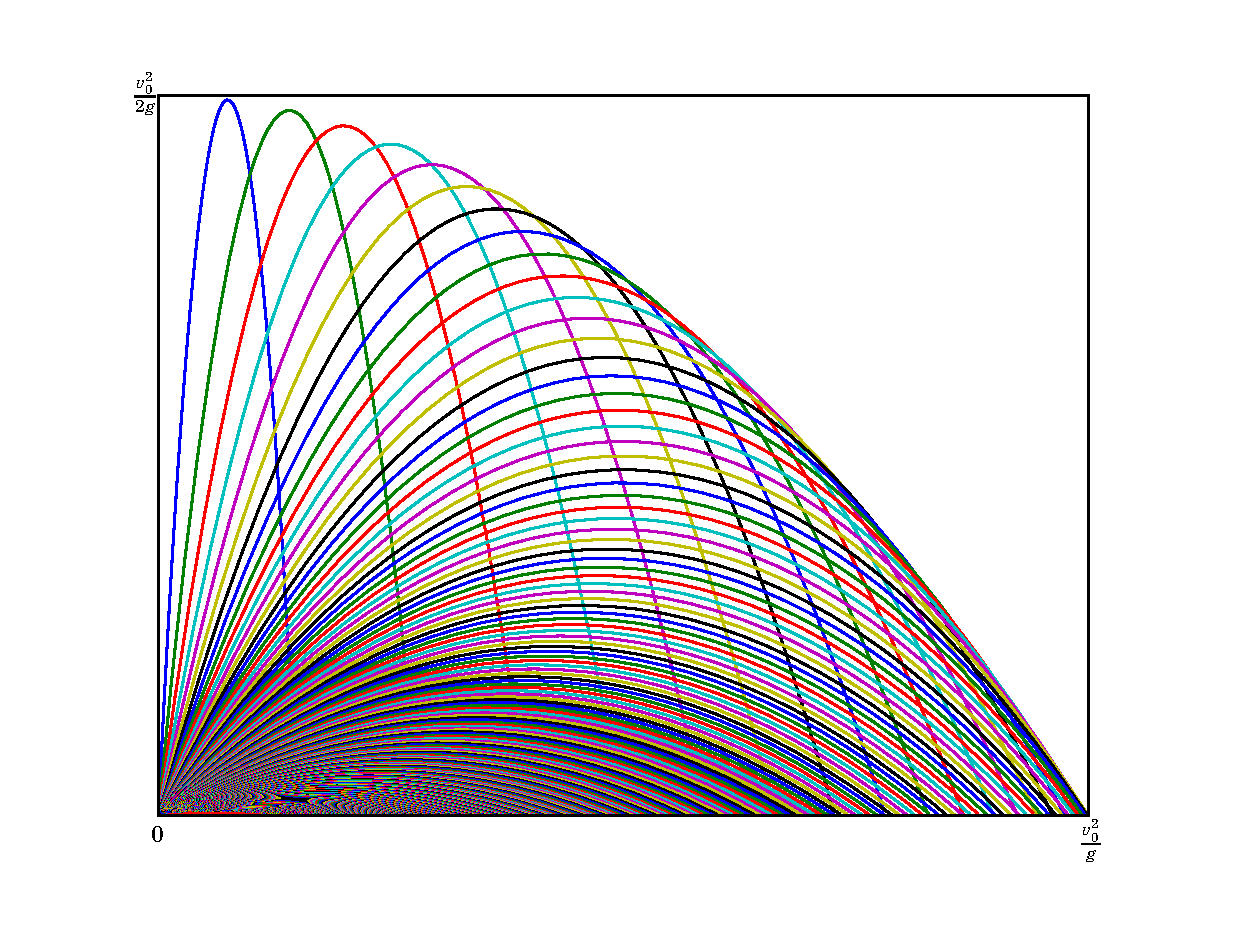
\includegraphics[scale=0.86]{coverplot}}
\newgeometry{left=0cm,top=0cm,bottom=0cm,right=0.5in}
\begin{flushright}
\begin{tikzpicture}[remember picture,overlay]
 \node[right] at (-15,-6) {
\includegraphics[scale=1.0]{calcbookcovertitle}};
 \node[right] at (-16.5,-15) {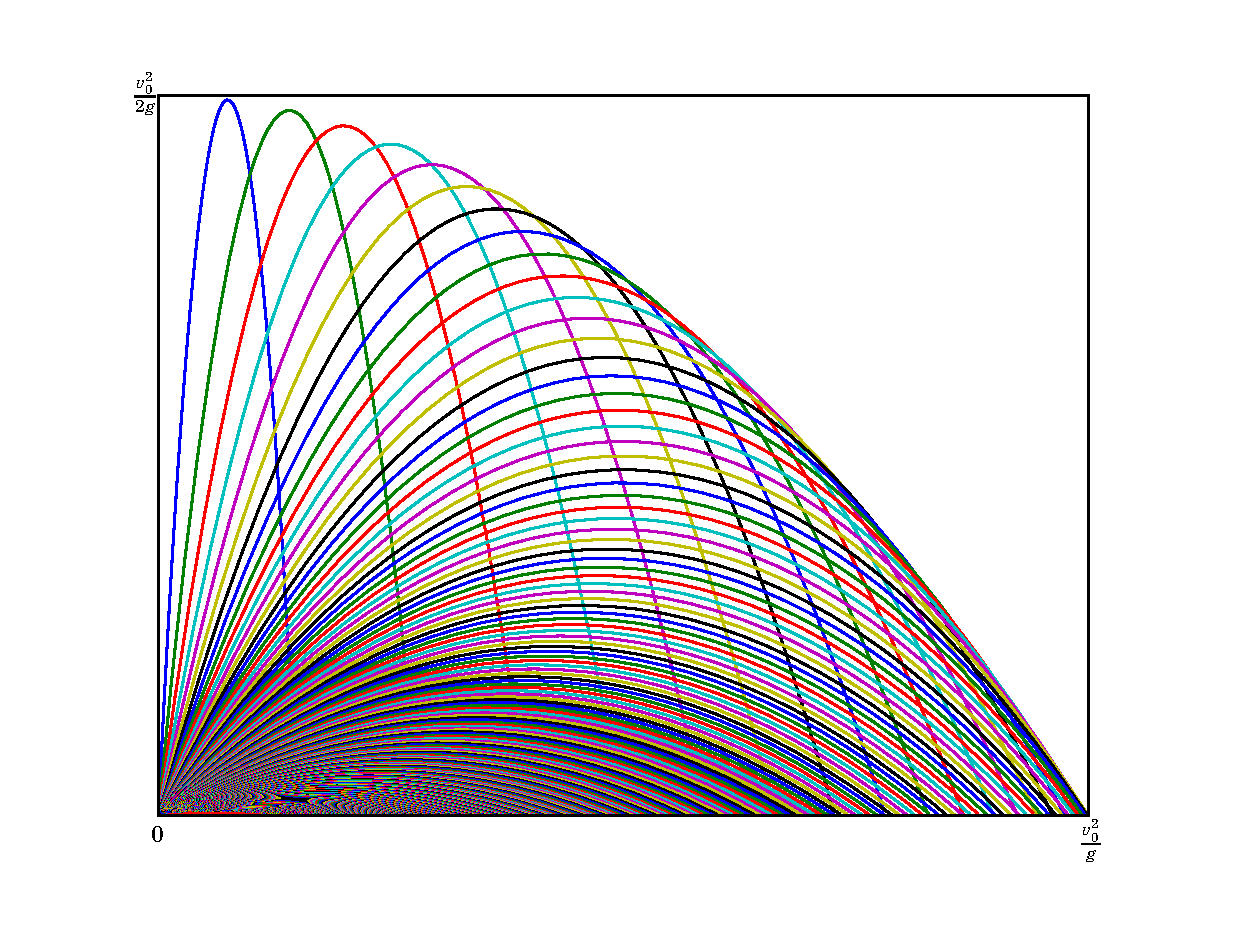
\includegraphics[scale=0.86]{coverplot}};
 \node[right] at (-4.5,-23) {
\includegraphics[scale=1.0]{calcbookcoverbottom}};
 \node[shape=rectangle,fill=mred,minimum height=\paperheight,minimum width=1.8in,anchor=west] at (current page.west) {};
\end{tikzpicture}
\end{flushright}
\restoregeometry
%Put the title page here
\title{Elementary Calculus}
\author{\textsf{\textbf{Michael Corral}}}
\date{\large \textsf{\textsl{Schoolcraft College}}}
%Put the author/copyright info here
\uppertitleback{\emph{About the author}:\\
Michael Corral is an Adjunct Faculty member of the Department of Mathematics at
Schoolcraft College. He received a B.A. in Mathematics from the University of
California, Berkeley, and received an M.A. in Mathematics and an M.S. in
Industrial \& Operations Engineering from the University of Michigan.\\\\
This text was typeset in \LaTeX\medspace with the \textsf{KOMA-Script} bundle,
using the GNU Emacs text editor on a
Fedora Linux system. The graphics were created using TikZ and Gnuplot.}
\lowertitleback{Copyright \copyright ~2020 ~Michael Corral.\\
Permission is granted to copy, distribute and/or modify this document
under the terms of the GNU Free Documentation License, Version 1.3
or any later version published by the Free Software Foundation;
with no Invariant Sections, no Front-Cover Texts, and no Back-Cover
Texts.}
\maketitle
\pagestyle{fancy}
\addtokomafont{footnotelabel}{\color{linecolor}}
\addtokomafont{footnotereference}{\color{linecolor}}
\renewcommand{\chaptermark}[1]{\markboth{#1}{}}
\renewcommand{\sectionmark}[1]{\markright{#1}}
\renewcommand{\qedsymbol}{\textsf{\textbf{\textsc{\small{QED}}}}}
\fancyhf{}
\setlength{\headheight}{22.26332pt}
\renewcommand{\headrulewidth}{0pt}
\newlength{\fminilength}%
\setlength{\fminilength}{\textwidth-2\fboxsep-2\fboxrule}%
\fancyhf{}
\fancyhead[LE]{\small\thepage}
\fancyhead[CE]{\small\scshape\leftmark}
\fancyhead[RO]{\small\thepage}
\fancyhead[CO]{\small\scshape\leftmark}
%Put the preface here
%\titleformat{\chapter}[display]
%  {\filcenter\huge\selectfont\bfseries\sffamily}
%  {}{0mm}{}[\vspace{3mm}\titlerule]
%\renewcommand*{\chapterformat}{\filcenter\huge\selectfont\bfseries\sffamily}
\titleformat{\chapter}[display]
  {\filcenter\huge\selectfont\bfseries\sffamily}
  {}{0mm}{\titlerule[1.5pt]\vspace{3mm}}[\vspace{3mm}{\titlerule[1.5pt]}]
\titleformat*{\section}{\Large\bfseries\sffamily}
\addchap{Preface}
This book covers calculus of a single variable. It is suitable for a year-long
(or two-semester) course, normally known as Calculus I and II in the United
States. The prerequisites are high school or college algebra, geometry and
trigonometry. The book is designed for students in engineering, physics,
mathematics, chemistry and other sciences.

One reason for writing this text was because I had already written its sequel,
\emph{Vector Calculus}. More importantly, I was dissatisfied with the current
crop of calculus
textbooks, which I feel are bloated and keep moving further away from the
subject's roots in physics. In addition, many of the intuitive
approaches and techniques from the early days of calculus---which I think often
yield more insights for students---seem to have been lost.

I agree with the views of the late
Russian mathematician V.I. Arnold on teaching mathematics, in particular the
idea that ``Mathematics is the part of physics where experiments are
cheap.''\footnote{\textsc{Arnold, V.I.},  ``On Teaching Mathematics'',
\emph{Russian Math. Surveys} 53 (1998), No. 1, 229-236. An HTML version is at
\url{https://www.uni-muenster.de/Physik.TP/~munsteg/arnold.html}}
The ties to physics are especially important in calculus, so this book tries to
introduce new concepts with physical motivations (what other motivations
can there be?). The book contains exercises and
examples that I hope will adequately prepare students who continue on in physics
and engineering.\footnote{The book covers some of the types of problems and
techniques for solving them that such students will likely encounter. Facility
with using named constants (e.g. $c$, $h$, $T$) is also emphasized.}

Perhaps controversially, the book uses infinitesimals, making it a
bit of a ``throwback'' or ``retro'' calculus text. My justification for this
heretical act was purely pedagogical: infinitesimals make learning calculus
easier, and their use aligns more with the way students will see calculus
in their physics, chemistry and other science classes and textbooks (where
infinitesimals are employed liberally). This might ruffle some feathers among
mathematical ``purists,'' but they are not the main audience for this book. That
said, the book is still compatible with the usual limit-based approach, so
an instructor could simply ignore the parts involving infinitesimals and teach
the material as he or she normally would. I did not want to be dogmatic, so I
used infinitesimals where I thought it made sense, and used limits where
appropriate (e.g. in discussing continuity, series). Again, pedagogy was my
priority.

The exercises at the end of each section are divided into three categories: A, B
and C. The A exercises are mostly of a routine computational nature, the B
exercises are slightly more involved, and the C exercises usually require some
effort or insight to solve. A crude way of describing A, B and C would be
``Easy'', ``Moderate'' and ``Challenging'', respectively. However, many of the B
exercises are easy and not all the C exercises are difficult.  Appendix A
provides answers and hints to many of the odd-numbered and some of the
even-numbered exercises.

A few exercises require the student to write a computer program to solve
numerical approximation problems (e.g. numerical methods for approximating
definite integrals). Algorithms are presented in pseudocode, with code
implementations in various languages (primarily Java, but also Python,
Octave, Sage). I hope the code comments will help the reader figure out what is
being done, regardless of familiarity with those languages. Students are free to
implement solutions using the language of their choice. There are no dedicated
``calculator exercises,'' as those have been rendered pointless by modern
computing (with which students need to become acquainted).

Stylistically I made a conscious effort to break from an unfortunate but all too
common mode of writing in mathematics texts, lamented in the preface of a
physics book: ``Nothing is more repellent to normal human beings than the
clinical succession of definitions, axioms, and theorems generated by the
labours of pure mathematicians.''\footnote{\textsc{Ziman, J.M.},
\emph{Elements of Advanced Quantum Theory}, Cambridge, U.K.: Cambridge
University Press, 1969.} I have been guilty of that sin myself, but I have
changed my ways and banished all traces of that sort of thing from this book. So
you won't find Definition 1.2, Theorem 3.3, Corollary 4.6, Lemma 5.7, Axiom 1B,
etc. Instead, I tried to borrow the best of the styles from the physics and
foreign languages textbooks I enjoyed so much in college. I also deliberately
avoided what the author Gore Vidal called the ``we-ness'' that
prevails in academic writing. There is no good reason for the ``royal we'' in a
textbook, and it comes off as a bit pompous, so \emph{we} won't use it.

This book is released under the GNU Free Documentation License (GFDL), which
allows others to not only copy and distribute the book but also to modify it.
For more details, see the included copy of the GFDL. So that there is no
ambiguity on this matter, anyone can make as many copies of this book as desired
and distribute it as desired, without needing my permission. The PDF version
will always be freely available to the public at no cost (go
to \url{http://www.mecmath.net/calculus}). Feel free to contact me at
\texttt{\href{mailto:mcorral@schoolcraft.edu}{mcorral@schoolcraft.edu}} for any
questions on this or any other matter regarding the book. I welcome your
feedback.

\begin{flushleft}
\emph{Schoolcraft College}\hspace{\stretch{1}}\textsc{Michael Corral}\\
\emph{December 2020}
\end{flushleft}

%\thispagestyle{empty}
\pdfbookmark[0]{\contentsname}{toc}
%Put the table of contents here
%\titlecontents{chapter}
%[0pt]
%{\addvspace{1.5pc}%
%\filright}
%{\selectfont\bfseries\sffamily\MakeUppercase{\chaptername} \thecontentslabel\\*[.2pc]%
%\large\selectfont\bfseries\sffamily}
%{}
%{\hfill\contentspage} % That is, without page number
%[\addvspace{.5pc}]
\tableofcontents
%Put a completely blank page here since the TOC has an odd number of pages
\clearpage{\pagestyle{empty}\section*{The Greek Alphabet}
\thispagestyle{empty}
\begin{tabular}{lll!{\qquad\qquad}lll!{\qquad\qquad}lll}
\hline\\[0.5pt]
\multicolumn{2}{l}{\textbf{Letters}} & \textbf{Name} & \multicolumn{2}{l}{\textbf{Letters}} &
 \textbf{Name} & \multicolumn{2}{l}{\textbf{Letters}} & \textbf{Name}\\[6pt]
A & $\alpha$ & alpha & I & $\iota$ & iota & P & $\rho$ & rho\\
B & $\beta$ & beta & K & $\kappa$ & kappa & $\Sigma$ & $\sigma$ & sigma\\
$\Gamma$ & $\gamma$ & gamma & $\Lambda$ & $\lambda$ & lambda & T & $\tau$ & tau\\
$\Delta$ & $\delta$ & delta & M & $\mu$ & mu & $\Upsilon$ & $\upsilon$ & upsilon\\
E & $\epsilon$ & epsilon & N & $\nu$ & nu & $\Phi$ & $\phi$ & phi\\
Z & $\zeta$ & zeta & $\Xi$ & $\xi$ & xi & X & $\chi$ & chi\\
H & $\eta$ & eta & O & $o$ & omicron & $\Psi$ & $\psi$ & psi\\
$\Theta$ & $\theta$ & theta & $\Pi$ & $\pi$ & pi & $\Omega$ & $\omega$ & omega\\[0.5pt]\\
\hline
\end{tabular}
\section*{Mathematical Notation}
\begin{tabular}{@{}c!{\qquad}l!{\quad\quad}l@{}}
\hline\\[0.5pt]
\textbf{Symbol} & \textbf{Meaning} & \textbf{Example}\\[6pt]
$\Rightarrow$ & if...then; implies & $\abs{x} > 1 ~\Rightarrow~ x^2 > 1$\\[3pt]
$\Leftrightarrow$ & if and only if; two-way implication & $\abs{x} > 1 ~\Leftrightarrow~ x^2 > 1$\\[3pt]
iff & if and only if; two-way implication & $\abs{x} > 1$ iff $x^2 > 1$\\[3pt]
$\nRightarrow$ & does not imply & $\abs{x} > 1 ~\nRightarrow~ x > 1$\\[3pt]
$\exists$ & there exists & $\exists$ a number $c > 0$\\[3pt]
$\nexists$ & there does not exist & $\nexists ~x$ such that $x^2 < 0$\\[3pt]
$\exists !$ & there exists a unique & $\exists !~x$ such that $2x-1=3$\\[3pt]
$\forall$ & for every & $\forall x \ge 0$, $\sqrt{x}$ is a real number\\[3pt]
$\equiv$ & is identically equal to & $f \equiv 0 ~\Rightarrow~ f(x)=0$ for all $x$\\[3pt]
$\propto$ & is proportional to & $y ~\propto x^2 ~\Rightarrow~ y=kx^2$ for some $k$\\[3pt]
$\subseteq$ & is a subset of & $\lbrace 0,1 \rbrace \subseteq \lbrace 0,1,2 \rbrace$\\[3pt]
%$\nsubseteq$ & is not a subset of & $\lbrace 0,1 \rbrace \nsubseteq \lbrace 2,3 \rbrace$\\[3pt]
$\in$ & is an element of & $1 \in \lbrace 1,2,3 \rbrace$\\[3pt]
$\notin$ & is not an element of & $1 \notin \lbrace 2,3 \rbrace$\\[3pt]
$\cup$ & union of sets & $\lbrace 0,1 \rbrace \cup \lbrace 2,3 \rbrace = \lbrace 0,1,2,3 \rbrace$\\[3pt]
$\cap$ & intersection of sets & $\lbrace 0,1 \rbrace \cap \lbrace 1,2 \rbrace = \lbrace 1 \rbrace$\\[3pt]
$\varnothing$ & empty set & $\lbrace 0,1 \rbrace \cap \lbrace 2,3 \rbrace = \varnothing$\\[3pt]
$\therefore$ & therefore & $\therefore$ $n$ must exist\\[0.5pt]\\
\hline
\end{tabular}
}

\mainmatter
\fancyhf{}
\fancyhead[LE]{\tikzstyle{headbox} = [fill=headercolor,line width=0pt,rectangle,
 rounded corners]
 \begin{tikzpicture}
  \node [headbox] (box){%
   \begin{minipage}{\fminilength}%
     \sffamily{\bfseries\thepage\qquad Chapter \thechapter}\enskip $\bullet$
      \enskip\leftmark\hfill{\bfseries\S\thesection}
    \end{minipage}%
  };
 \end{tikzpicture}}
\fancyhead[LO]{\tikzstyle{headbox} = [fill=headercolor,line width=0pt,rectangle,
 rounded corners]
 \begin{tikzpicture}
  \node [headbox] (box){%
   \begin{minipage}{\fminilength}%
     \sffamily {}\hfill\rightmark\enskip $\bullet$ \enskip{\bfseries{Section
     \thesection\qquad\thepage}}
    \end{minipage}%
  };
 \end{tikzpicture}}
%\titleformat{\chapter}[display]
%  {\filcenter\LARGE\selectfont\bfseries\sffamily}
%  {CHAPTER \thechapter}{3mm}{\titlerule\vspace{3mm}\huge}
\titleformat{\chapter}[display]
  {\filcenter\LARGE\selectfont\bfseries\sffamily}
  {\titlerule[1.5pt]\vspace{3mm}\MakeUppercase{\chaptertitlename}
   \thechapter}{3mm}
  {\titlerule[1.5pt]\vspace{3mm}\huge}
%Put the main chapters here
\chapter{The Derivative}
%Begin Section 1.1
\section{Introduction}
Calculus can be thought of as the analysis of curved shapes.\footnote{It is more
than that, of course, but that definition puts us in good company:
the first European textbook on calculus, written by the French mathematician
Guillaume de l'H\^{o}pital in 1696, was titled \emph{Analyse des Infiniment
Petits pour l'Intelligence des Lignes Courbes} (which translates as
\emph{Analysis of the Infinitely Small for Understanding Curved Lines}). That
book (in French) can be obtained freely in electronic form at
\url{https://archive.org}}
Its development grew out of attempts to solve physical problems.
For example, suppose that an object at rest 100 ft above the ground is dropped.
Ignoring air resistance and wind, the object will fall straight down until it
hits the ground (see Figure \ref{fig:fall}(a)). As will be proved later,
$t$ seconds after being dropped the object will be
$s = s(t) = -16t^2 + 100$ ft above the ground. The object will thus hit
the ground after 2.5 seconds (when $s = 0$). While the object's \emph{path} is a
straight line, the graph of its position $s$ above the ground as a function of
time $t$ is curved, part of a parabola (see Figure \ref{fig:fall}(b)).

\begin{figure}[ht]
 \centering
 \subfloat[][ Path of the object]{
 \begin{tikzpicture}[>=latex,every node/.style={font=\small}]
  \draw [line width=1pt,<->] (-1,0) -- (-1,3)
   node[midway,fill=white] {$100$ ft};
  \draw [dashed,line width=1pt,->] (0,3) -- (0,0)
   node [right,pos=0.0] {$~t=0$ sec} node [below right,pos=1.0] {$t=2.5$ sec};
  \draw [line width=1.2pt] (-2,0) -- (2.5,0);
  \fill (0,3) circle (2.5pt);
  \node [right] at (0.2,1.5) {object falling};
 \end{tikzpicture}}
 \qquad\qquad
 \subfloat[][ Position $s$ as a function of time $t$]{
 \begin{tikzpicture}[>=latex,every node/.style={font=\small}]
  \node[below left] at (0,0) {$0$};
  \draw [linecolor,line width=1.5pt] (0,3) parabola (2.5,0);
  \node[right] at (1.8,1.85) {$s=-16t^2 + 100$};
  \draw [<->,black!60,line width=1pt] (0,3.8) node[above] {$s$}
   |- (5.5,0) node[right] {$t$};
  \fill (0,3) circle (2.5pt);
  \fill (2.5,0) circle (2.5pt);
  \node [left] at (0,3) {$100$};
  \node [below] at (2.5,0) {$2.5$};
 \end{tikzpicture}}
 \caption[]{\quad An object dropped from 100 ft above the ground}
 \label{fig:fall}
\end{figure}

How fast is the object moving before it hits the ground? This is where
calculus comes in. The solution, presented now, will motivate much of this
chapter.\index{straight line motion}

First, the object travels 100 ft in 2.5 seconds, so its \textbf{average speed}
in that time is\index{speed}
\begin{displaymath}
 \frac{\text{distance traveled}}{\text{time elapsed}} ~=~
 \frac{100 \text{ ft}}{2.5 \text{ seconds}} ~=~ 40 \text{ ft/s,}
\end{displaymath}
and its \textbf{average velocity}\index{velocity!average} in that time is
\begin{displaymath}
 \frac{\text{change in position}}{\text{change in time}} ~=~
 \frac{\text{final position} ~-~ \text{initial position}}
 {\text{end time} ~-~ \text{start time}} ~=~
 \frac{0 \text{ ft} ~-~ 100 \text{ ft}}{2.5 \text{ sec} ~-~ 0 \text{ sec}} ~=~
 -40 \text{ ft/s.}
\end{displaymath}
Unlike speed, velocity takes direction into account. Thus, the object's downward
motion means it has negative velocity. Positive velocity implies upward motion.

\par Using the idea of average velocity over an interval of time, there is a
natural way to define the object's
\textbf{instantaneous velocity}\index{velocity!instantaneous}\index{velocity}
at a particular \emph{instant} of time $t$:
\begin{enumerate}
 \item Find the average velocity over an interval of time.
 \item Let the interval become smaller and smaller indefinitely, shrinking
  to a point $t$. If the average velocity over that smaller and smaller
  interval approaches some value, call that value the instantaneous velocity
  at time $t$.
\end{enumerate}
Figure \ref{fig:instvel} below shows how to choose the interval: for any
time $t$ between 0 and 2.5, use the interval $\ival{t}{t+\Delta t}$, where
$\Delta t$ (pronounced ``delta t'') is a small positive number. So $\Delta t$
is the change in time over the interval; denote by $\Delta s$ the change in the
position $s$ over that interval.

\begin{figure}[ht]
 \begin{center}
 \begin{tikzpicture}[>=latex,every node/.style={font=\small}]
  \draw [linecolor,line width=1.5pt] (0,4) parabola (5,0);
  \draw[dotted] (2,1.44) -- (2,0);
  \draw[dotted] (4,1.44) -- (4,0);
  \draw[dotted] (2,1.44) -- (0,1.44);
  \draw[dotted] (2,3.36) -- (0,3.36);
  \draw [<->,black!60,line width=1pt,anchor=base] (0,4.8) node[above]
   {$s$} |- (7.5,0) node[right] {$t$}
   node[black,shift={(0,-0.4)}] at (2,0) {$t$}
   node[black,shift={(0,-0.4)}] at (4,0) {$t + \Delta t$}
   node[black,shift={(0,-0.4)}] at (5,0) {$2.5$};
  \fill (0,4) circle (2.5pt);
  \fill (5,0) circle (2.5pt);
  \node[below left] at (0,0) {$0$};
  \node [left] at (0,4) {$100$};
  \fill (2,3.36) circle (2.5pt);
  \fill (4,1.44) circle (2.5pt);
  \draw[dashed] (2,3.36) -- (4,1.44) -- (2,1.44) node[midway,below] {$\Delta t$}
   -- (2,3.36) node[midway,left] {$\Delta s$};
  \draw (2.3,1.44) -- ++(0,0.3) -- ++(-0.3,0);
  \node [left] at (0,1.44) {$s(t + \Delta t)$};
  \node [left] at (0,3.36) {$s(t)$};
  \node [right] at (4,2.6) {average velocity $= \dfrac{\Delta s}{\Delta t} =
  \dfrac{s(t + \Delta t) ~-~ s(t)}{\Delta t}$};
 \end{tikzpicture}\vspace{-4mm}
 \end{center}
 \caption[]{\quad Average velocity $\frac{\Delta s}{\Delta t}$ over the interval
  $\ival{t}{t+\Delta t}$}
 \label{fig:instvel}
\end{figure}

The average velocity of the object over the interval $\ival{t}{t+\Delta t}$ is
$\frac{\Delta s}{\Delta t}$, so since $s(t) = -16t^2 + 100$:

\begin{align*}
 \dfrac{\Delta s}{\Delta t} ~~&=~~ \dfrac{s(t + \Delta t) ~-~ s(t)}
  {\Delta t}\\[8pt]
  &=~~ \dfrac{-16(t+\Delta t)^2 ~+~ 100 ~-~ (-16t^2 ~+~ 100)}{\Delta t}\\[8pt]
  &=~~ \dfrac{-16t^2 ~-~ 32t\Delta t ~-~ 16(\Delta t)^2 ~+~ 100 ~+~ 16t^2
   ~-~ 100}{\Delta t}\\[8pt]
  &=~~ \dfrac{-32t\Delta t ~-~ 16(\Delta t)^2}{\Delta t}
   ~~=~~ \dfrac{\cancel{\Delta t} \,(-32t ~-~ 16\Delta t)}
          {\cancel{\Delta t}}\\[6pt]
  &=~~ -32t ~-~ 16\Delta t ~,
\end{align*}
Now let the interval $\ival{t}{t+\Delta t}$ get smaller and
smaller indefinitely---that is, let $\Delta t$ get closer and closer to 0.
Then the average velocity $\frac{\Delta s}{\Delta t} = -32t - 16\Delta t\,$
gets closer and closer to $-32t - 0 = -32t$. Thus, \emph{the object has
instantaneous velocity $-32t$ at time $t$}. This calculation can be
interpreted as taking the \textbf{limit}\index{limit} of
$\frac{\Delta s}{\Delta t}\,$ \emph{as} $\Delta t\,$ \emph{approaches} $0$,
written as follows:
\begin{align*}
 \text{instantaneous velocity at $t$} ~~&=~~
  \text{limit of average velocity over $\ival{t}{t+\Delta t}$
  as $\Delta t$ approaches to 0}\\[6pt]
  &=~~ \lim_{\Delta t \to 0} ~\frac{\Delta s}{\Delta t}\\[8pt]
  &=~~ \lim_{\Delta t \to 0} ~(-32t ~-~ 16\Delta t)\\[6pt]
  &=~~ -32t - 16(0)\\[6pt]
  &=~~ -32t
\end{align*}

Notice that $\Delta t$ is not replaced by $0$ in the
ratio $\frac{\Delta s}{\Delta t}$ until \emph{after} doing as much cancellation
as possible. Notice also that the instantaneous velocity of the object
varies with $t$, as it should (why?). In particular, at the instant when the
object hits the ground at time $t = 2.5$ sec, the instantaneous velocity is
$-32(2.5) = -80$ ft/s.

If this makes sense so far, then you understand the crux of the idea of what a
limit is and how to calculate a limit. The instantaneous velocity $v(t) = -32t$
is called the \textbf{derivative} of the position function $s(t) =-16t^2 + 100$.
Calculating derivatives, analyzing their properties, and using them to solve
various problems are part of \emph{differential calculus}.\index{derivative}

What does this have to do with curved shapes? Instantaneous velocity is a
special case of an \textbf{instantaneous rate of change}\index{instantaneous
rate of change} of a function; in this case the instantaneous rate of change of
the position (height above the ground) of the object. Similar to how the rate
of change of a line is its slope, the instantaneous rate of change of a general
curve represents the \textbf{slope of the curve}. For example, the parabola
$s(t) = -16t^2 + 100$ has slope $-32t$ for all $t$. Note that the slope of this
curve varies (as a function of $t$), unlike the slope of a straight line.

Finding the area inside curved regions is another type of problem that calculus
can solve. The basic idea is to use simpler regions---rectangles---whose areas
are known, then use those to approximate the area inside the curved
region. One such method is to draw more and more rectangles of diminishing
widths \emph{inside} the curved region,\footnote{It will be
shown later (in Chapter 5) that the rectangles do not have to be completely
inside the region.} so that the sums of their areas approach the area of the
curved region. Figure \ref{fig:area} shows an example with four
rectangles to approximate the area under a curve $y=f(x)$ over an interval
$\ival{a}{b}$ on which $f(x) \ge 0$.

\begin{figure}[ht]
 \begin{center}
  \begin{tikzpicture}[>=latex,every node/.style={font=\small}]
   \fill [fill=fillcolor] (4.2,1) to[out=140,in=-10] (3,1.5)
    to[out=180,in=0] (2,1) to[out=180,in=-45] (1,1.5) -- (1,0) -- (4.2,0) --
    (4.2,1);
   \draw[line width=1pt] (1,0) -- (1,1.5);
   \draw[line width=1pt] (4.2,0) -- (4.2,1);
   \draw [linecolor,line width=1.5pt] (4.2,1) to[out=140,in=-10] (3,1.5)
    to[out=180,in=0] (2,1) to[out=180,in=-45] (1,1.5);
   \node [above] at (2.5,1.5) {$y = f(x)$};
   \draw [dashed] (1.5,0) -- (1.5,1.125) -- (1,1.125);
   \draw [dashed] (1.5,1) -- (2.5,1);
   \draw [dashed] (2.5,0) -- (2.5,1.26) -- (3.85,1.26) -- (3.85,0);
   \draw [dashed] (3.85,1) -- (4.2,1);
   \draw[<->,black!60,line width=1pt,anchor=base] (0,2.3) node[above] {$y$} |-
    (5,0) node[right] {$x$} node[black,shift={(0,-0.4)}] at (1,0) {$a$}
    node[black,shift={(0,-0.4)}] at (4.2,0) {$b$};
   \fill (1,1.5) circle (2.5pt);
   \fill (4.2,1) circle (2.5pt);
  \end{tikzpicture}\vspace{-6mm}
 \end{center}
 \caption[]{\quad The area of a curved region}
 \label{fig:area}
\end{figure}

The limit of these sums of rectangular areas is called an \textbf{integral}.
The study and application of integrals are part of
\emph{integral calculus}.\index{integral} Perhaps the most remarkable result in
calculus is that there is a connection between derivatives and integrals---the
\emph{Fundamental Theorem of Calculus}, discovered
in the 17\textsuperscript{th} century, independently, by the two men who
invented calculus as we know it: English physicist, astronomer and
mathematician Isaac Newton (1642-1727) and German mathematician and philosopher
Gottfried Wilhelm von Leibniz (1646-1716).

Calculus makes extensive use of \emph{infinite sequences and
series}\index{sequence}\index{series}\index{infinite series}. An
\textbf{infinite series} is just a sum of an infinite number of terms. For
example, it will be shown later in the text that
\begin{equation}\label{eqn:piseries}
 \frac{\pi}{4} ~~=~~ 1 ~-~ \frac{1}{3} ~+~ \frac{1}{5} ~-~ \frac{1}{7} ~+~
 \frac{1}{9} ~-~ \cdots ~,
\end{equation}
where the sum on the right involves an infinite number of terms. A \textbf{power
series}\index{power series} is a particular type of infinite series applied to
functions; it can be thought of as a polynomial of infinite degree. For example,
the trigonometric function $\sin\;x$ does not appear to be a polynomial. But it
turns out that $\sin\;x$ has a power series representation as
\begin{equation}\label{eqn:sinseries}
 \sin\,x ~~=~~ x ~-~ \frac{x^3}{3!} ~+~ \frac{x^5}{5!} ~-~ \frac{x^7}{7!} ~+~
 \frac{x^9}{9!} ~-~ \cdots ~,
\end{equation}
where again the sum continues infinitely, and the formula holds for all $x$ (in
radians).

The idea of replacing a function by its power series played an important role
throughout the development of calculus, and is a powerful technique in many
applications.

All the functions in this text will be functions of a single real
variable---that is, the values that the variable can take are real
numbers. Below is some standard notation for commonly-used sets
of numbers:\index{real numbers}\index{$\mathbb{R}$}\index{rational
numbers}\index{$\mathbb{Q}$}\index{integers}
\index{$\mathbb{I}$}\index{natural numbers}\index{$\mathbb{N}$}

\begin{align*}
 \Naturals ~~&=~~ \text{the set of all \textbf{natural} numbers, i.e. the set of
  nonnegative integers: } 0, 1, 2, 3, 4, \ldots\\[6pt]
 \Integers ~~&=~~ \text{the set of all integers: } 0, \pm 1, \pm 2, \pm 3,
  \pm 4, \ldots\\[6pt]
 \Rationals ~~&=~~ \text{the set of all \textbf{rational} numbers $\frac{m}{n}$,
  where $m$ and $n$ are integers, with $n \ne 0$}\\[6pt]
 \Reals ~~&=~~ \text{the set of all real numbers}
\end{align*}
Note that $\Naturals ~~\subset~~ \Integers ~~\subset~~ \Rationals ~~\subset~~
\Reals$.

The set of real numbers consists of the rational numbers together with numbers
that are not rational, called \textbf{irrational numbers}.\index{irrational
numbers} For example, $\sqrt{2}$ is irrational. That is, 2 is not the square of
a rational number. In fact, if the square of a rational number $q$ were an
integer, then $q$ itself would have to be an integer: write $q$ as $m/n$, where
$m$ and $n$ are positive integers with no common positive integer divisors other
than 1. Since $q^2 = m^2/n^2$ simply duplicates the integer divisors of $m$ and
$n$, then $q^2$ can be an integer only if $n=1$, i.e. $q$ is an integer. Clearly
2 is not the square of an integer, and thus it cannot be the square of a
rational number. This argument also shows that $\sqrt{3}$, $\sqrt{5}$,
$\sqrt{6}$, $\sqrt{7}$, $\sqrt{8}$, $\sqrt{10}$, and so on, are
irrational.\footnote{This argument is due to the British philosopher Bertrand
Russell (1872-1970). For an alternative proof that $\sqrt{2}$ is irrational, see
pp. 97-98 in \textsc{Gelfand, I.M. and A. Shen}, \emph{Algebra}, Boston:
Birkh\"{a}user, 1993.}

It turns out that there are far more irrational numbers--and hence real
numbers---than rational numbers. In fact, whereas the rational numbers can be
listed in a sequence (i.e. first, second, third, etc.), the set of real numbers
cannot.\footnote{For a proof see Ch.1 in \textsc{Kamke, E.}, \emph{Theory of
Sets}, New York: Dover Publications, Inc., 1950.} For example, in the closed
interval $\ival{0}{1}$ there is no ``next'' real number after the number $0$.
Thus, some infinite sets are larger than others---$\Reals$ is larger than
$\Rationals$. Intervals such as $\ival{0}{1}$
or $\Reals$ itself are examples of a \emph{continuum} of objects, i.e. no
gaps exist.\footnote{For a study of the structure of the real number system, see
\textsc{Burrill, C.W.}, \emph{Foundations of Real Numbers}, New York:
McGraw-Hill Book Company, 1967.}
A famous unsolved problem in mathematics---the \emph{Continuum Hypothesis}---is
whether an infinite set exists that is larger in size than $\Rationals$ but
smaller than $\Reals$.

\emph{Infinity} is an important notion in calculus. Whether it is the idea
of \emph{infinitely large} or \emph{infinitesimally small}, calculus attempts to
give the idea some mathematical meaning (typically by way of
limits).\footnote{Not everyone agrees that calculus does this satisfactorily.
For example, for an alternative development of basically the same material
in ``standard'' calculus but without the use of limits---called
\emph{infinitesimal analysis}---see \textsc{Keisler, H.J.}, \emph{Elementary
Calculus: An Infinitesimal Approach}, Boston: Prindle, Weber \& Schmidt, 1976.}
The mathematical use of infinity has been a subject of philosophical
debate.\footnote{For example, see the essays by L. E. J. Brouwer, Hermann
Weyl and David Hilbert in \textsc{Heijenoort, J. van}, \emph{From Frege to
G{\"o}del: A Source Book in Mathematical Logic, 1879-1931}, Cambridge, MA:
Harvard University Press, 1967.}

Though several centuries old, calculus was the beginning of \emph{modern}
mathematics. \emph{Classical} mathematics (e.g. algebra, geometry,
trigonometry)---whose origins date back to the ancient Babylonians, Egyptians,
and Greeks---was concerned mostly with the study of \emph{static} quantities.
Calculus produced a way to analyze \emph{dynamic} (i.e. changing) quantities.
The period from the 17\textsuperscript{th} through the 19\textsuperscript{th}
century also saw revolutionary advances in physics, chemistry, biology and other
sciences. The birth of calculus was one part of that qualitative leap.
\newpage
\startexercises\label{sec1dot1}
{\small
\probs{A}
\par\noindent For Exercises 1-4, suppose that an object moves in a straight line
such that its position $s$ after time $t$ is the given function $s=s(t)$. Find
the instantaneous velocity of the object at a general time $t \ge 0$.
You should mimic the earlier example for the instantaneous velocity when
$s = -16t^2 + 100$.
\begin{enumerate}[\bfseries 1.]
 \begin{multicols}{4}
  \item $s = t^2$
  \item $s = 9.8t^2$
  \item $s = -16t^2 + 2t$
  \item $s = t^3$
 \end{multicols}
 \item By equation (\ref{eqn:piseries}), $\pi ~=~ 4\,\left(1 ~-~ \frac{1}{3} ~+~
  \frac{1}{5} ~-~ \frac{1}{7} ~+~ \frac{1}{9} ~-~ \cdots ~\right)$, where the
  $n^{th}$ term in the sum inside the parentheses is $\frac{(-1)^{n+1}}{2n-1}$
  (starting at $n=1$).\footnote{This, by the way, is a terrible formula
  for calculating $\pi$; getting just the 3.14 part requires 119 terms in the
  sum!} So the first approximation of $\pi$ using this formula is
  $\pi \approx 4\,(1) = 4.0$, and the second approximation is $\pi \approx
  4\,\left(1 - \frac{1}{3}\right) = 8/3 \approx 2.66667$. Continue like this
  until two consecutive approximations have $3$ as the first digit before the
  decimal point. How many terms in the sum did this require? Be careful with
  rounding off in the approximations.
\suspend{enumerate}
\probs{B}
\resume{enumerate}[{[\bfseries 1.]}]
 \item In elementary geometry you learned that the area inside a circle of
  radius $r>0$ is $\pi r^2$ (that formula will be proved later in the text). So
  in particular, let $C$ be a circle of radius $1$. Then the area inside $C$ is
  $\pi$. That area can be approximated by \emph{Eudoxus' method of
  exhaustion}.\index{Eudoxus}\index{method of exhaustion}\footnote{Originally
  due  to another ancient Greek mathematician, Antiphon (ca. 430 \textsc{b.c.})}
  The idea is to inscribe \emph{regular polygons}\index{regular polygon} inside
  the circle, i.e. the vertexes of the polygons touch $C$. Recall from geometry
  that a polygon is regular if its sides are of equal length. By increasing the
  number of sides of the polygons, the areas inside the polygons will approach
  the area ($\pi$) of $C$. This was an early attempt at using what is now
  called a limit.\footnote{The great ancient Greek mathematician, physicist and
  astronomer Archimedes (ca. 287-212 \textsc{b.c.}) used this method, together
  with circumscribed regular polygons, to calculate $\pi$.}

\begin{figure}[ht]
\begin{minipage}[b]{7.5cm}
 \begin{center}
  \begin{tikzpicture}[every node/.style={font=\small}]
   \filldraw [linecolor,fill=fillcolor,line width=1pt] (45:1.5) -- (135:1.5) --
    (225:1.5) -- (315:1.5) -- cycle;
   \draw [line width=1pt] (0,0) circle (1.53);
   \draw [linecolor,dashed] (0,0) -- (45:1.5) node[black,midway,below] {$1$};
   \fill (0,0) circle (2pt);
   \node [left] at (150:1.58) {$C$};
  \end{tikzpicture}\vspace{-5mm}
 \end{center}
 \caption[]{\quad Inscribed square}
 \label{fig:insquare}
\end{minipage}
\begin{minipage}[b]{7.5cm}
 \begin{center}
  \begin{tikzpicture}[every node/.style={font=\small}]
   \filldraw [linecolor,fill=fillcolor,line width=1pt] (0:1.5) -- (60:1.5) --
    (120:1.5) -- (180:1.5) -- (240:1.5) -- (300:1.5) -- cycle;
   \draw [line width=1pt] (0,0) circle (1.53);
   \draw [linecolor,dashed] (0,0) -- (1.5,0) node[black,pos=0.4,above] {$1$};
   \fill (0,0) circle (2pt);
   \node [left] at (150:1.58) {$C$};
  \end{tikzpicture}\vspace{-5mm}
 \end{center}
 \caption[]{\quad Inscribed regular hexagon}
 \label{fig:inhexagon}
\end{minipage}
\end{figure}\vspace{-2mm}

 \begin{enumerate}[\bfseries (a)]
  \item Inscribe a square inside $C$, as in Figure \ref{fig:insquare}. Show that
   the area inside the square is $2$. This is a poor approximation of $\pi =
   3.14159265...$, obviously.
  \item Inscribe a regular hexagon ($6$-sided)
   inside $C$, as in Figure \ref{fig:inhexagon}. Show that the area inside the
   hexagon is $\frac{3\,\sqrt{3}}{2} \approx 2.59807621$. This is a slightly
   better---though still poor---approximation of $\pi$.
  \item Inscribe a regular dodecagon ($12$-sided) inside $C$. Show that the
   area inside the dodecagon is $3$. It thus takes $12$ sides for the
   approximation to get the first digit of $\pi$ correct.
  \item Inscribe a regular $100$-sided polygon inside $C$. Show that the area
   inside this polygon is approximately $3.13952598$. This is getting closer to
   $\pi$.
  \item Show that the general formula for the area inside a regular $n$-sided
   polygon inscribed inside $C$ is $\dfrac{n}{2}\,\sin\,\left(
   \dfrac{360\Degrees} {n}\right)$. \emph{(Hint: The double-angle identity
   $\sin\,2\theta = 2\,\sin\,\theta\;\cos\,\theta$ might help.)}
 \end{enumerate}
\newpage
\suspend{enumerate}
\probs{C}
\resume{enumerate}[{[\bfseries 1.]}]
 \item What is the flaw in the following ``proof'' that $\pi = 4$?:

\parpic[r]{\begin{tikzpicture}[every node/.style={font=\small}]
 \filldraw [linecolor,fill=fillcolor,line width=1pt] (0,0) circle (1.5);
 \draw [linecolor,dashed] (-1.5,0) -- (1.5,0) node[black,midway,above] {$d =1$};
 \draw [black,line width=1pt] (-1.5,1.5) rectangle (1.5,-1.5);
\end{tikzpicture}}
\noindent\textbf{Step 1:} Draw a square around a circle of diameter $d = 1$.
The circumference of the circle is thus $\pi\,d = \pi$, and the perimeter of the
square is 4.\vspace{29mm}

\parpic[r]{\begin{tikzpicture}[every node/.style={font=\small}]
 \draw [black!60,dotted,line width=0.75pt] (-1.5,1.5) rectangle (1.5,-1.5);
 \filldraw [linecolor,fill=fillcolor,line width=1pt] (0,0) circle (1.5);
 \draw [linecolor,dashed] (-1.5,0) -- (1.5,0) node[black,midway,above] {$d =1$};
 \draw [black,line width=1pt] (-1.5,-1.09) -- (-1.5,1.09) -- (-1.09,1.09) --
  (-1.09,1.5) -- (1.09,1.5) -- (1.09,1.09) -- (1.5,1.09) -- (1.5,-1.09) --
  (1.09,-1.09) -- (1.09,-1.5) -- (-1.09,-1.5) -- (-1.09,-1.09) -- cycle;
\end{tikzpicture}}
\noindent\textbf{Step 2:} Remove corners from the square as shown in the picture
on the right, so that four new corners touch the circle. Notice that the
perimeter of the resulting polygon is still 4, since the lengths of the removed
corner pieces are duplicated in the new polygon, so that the lengths of all the
vertical sides add up to 2 while the lengths of all the horizontal sides add up
to 2.\vspace{17mm}

\parpic[r]{\begin{tikzpicture}[every node/.style={font=\small}]
 \draw [black!60,dotted,line width=0.75pt] (-1.09,1.5) rectangle (1.09,-1.5);
 \draw [black!60,dotted,line width=0.75pt] (-1.5,1.09) rectangle (1.5,-1.09);
 \filldraw [linecolor,fill=fillcolor,line width=1pt] (0,0) circle (1.5);
 \draw [linecolor,dashed] (-1.5,0) -- (1.5,0) node[black,midway,above] {$d =1$};
 \draw [black,line width=1pt] (-1.5,-0.84) -- (-1.5,0.84) -- (-1.29,0.84) --
  (-1.29,1.09) -- (-1.09,1.09) -- (-1.09,1.29) -- (-0.84,1.29) -- (-0.84,1.5) --
  (0.84,1.5) -- (0.84,1.29) -- (1.09,1.29) -- (1.09,1.09) -- (1.29,1.09) --
  (1.29,0.84) -- (1.5,0.84) -- (1.5,-0.84) -- (1.29,-0.84) -- (1.29,-1.09) --
  (1.09,-1.09) -- (1.09,-1.29) -- (0.84,-1.29) -- (0.84,-1.5) -- (-0.84,-1.5) --
  (-0.84,-1.29) -- (-1.09,-1.29) -- (-1.09,-1.09) -- (-1.29,-1.09) --
  (-1.29,-0.84) -- cycle;
\end{tikzpicture}}
\noindent\textbf{Step 3:} Remove corners from the polygon in Step 2, as shown in
the picture on the right, so that eight new corners touch the circle. The
perimeter of the resulting polygon is again still 4.\vspace{25mm}

\parpic[r]{\begin{tikzpicture}[every node/.style={font=\small}]
 \filldraw [linecolor,fill=fillcolor,line width=1pt] (0,0) circle (1.48);
 \draw [linecolor,dashed] (-1.5,0) -- (1.5,0) node[black,midway,above] {$d =1$};
 \draw [black,line width=1pt] (0,0) circle (1.51);
\end{tikzpicture}}
\noindent\textbf{Step 4:} Continue this procedure indefinitely, with each
successive polygon still having a perimeter of 4 and becoming increasingly
indistinguishable from the circle. Since the perimeters of the polygons always
equal 4 and approach the circle's circumference ($\pi$), then $\pi$ must equal
4.\vspace{18mm}
\picskip{7}

% \noindent\emph{(Hint: Think of the key difference between this problem and the
% approximations to $\pi$ in Exercise 6.)}
 \item An infinite set is \textbf{countable}\index{countable} if its members can
  be put into a one-to-one correspondence with the members of $\Naturals$, the
  set of natural numbers ($0, 1, 2, 3, 4, \ldots$). Clearly $\Naturals$ is
  itself countable. The set $\Integers$ of all integers is also countable, by
  means of the following one-to-one correspondence with $\Naturals$:
\begin{center}
 \small{\begin{tabular}{|>{\columncolor[gray]{0.8}}c|c|c|r|c|r|c|r|c|r|c|}
 \hline
 $\Naturals$ & 0 & 1 & 2 & 3 & 4 & 5 & 6 & 7 & 8 & $\ldots$\\
 \hline
 $\Integers$ & 0 & 1 & -1 & 2 & -2 & 3 & -3 & 4 & -4 & $\ldots$\\
 \hline
 \end{tabular}}
\end{center}
\noindent Show that $\Rationals$ (the set of all rational numbers) is countable.
\emph{(Hint: The above correspondence for $\Integers$ is an infinite list in one
dimension (the horizontal direction). For $\Rationals$ think
two-dimensionally.)}
\end{enumerate}}
\newpage
%Begin Section 1.2
\section{The Derivative: Limit Approach}
The following definition generalizes the example from the previous section
(concerning instantaneous velocity) to a general function
$f(x)$:\index{$\Delta x$}\index{$f'$}\index{derivative}

\statedefn{defn:derivative}{
{The \textbf{derivative} of a real-valued function $f(x)$,
denoted by $f'(x)$, is
\begin{equation}\label{eqn:derivative}
 f'(x) ~=~ \lim_{\Delta x \to 0} ~\frac{\Delta f}{\Delta x} ~=~
  \lim_{\Delta x \to 0} ~\frac{f(x + \Delta x) ~-~ f(x)}{\Delta x}
\end{equation}
for $x$ in the domain of $f$, provided that the limit exists.\footnotemark
}
}\footnotetext{Recall that the \emph{domain}\index{domain} of $f$ is the set of
all numbers $x$ such that $f(x)$ is defined.}

For a general function $f(x)$, the derivative $f'(x)$ represents the
\textbf{instantaneous rate of change}\index{instantaneous rate of change} of $f$
at $x$, i.e. the rate at which $f$ changes at the ``instant'' $x$. For the limit
part of the definition only the intuitive idea of how to take a limit---as in
the previous section---is needed for now. Notice that the above definition makes
the derivative $f'$ itself a function of the variable $x$. The function $f'$ can
be evaluated at specific values of $x$, or you can write its general formula
$f'(x)$.

The (instantaneous) velocity of an object as the derivative of the object's
position as a function of time is only one physical application of derivatives.
There are many other examples:

\begin{center}
 \small{\begin{tabular}{|c|c|c|}
 \hline
 \rowcolor{fillcolor} Field & Function & Derivative\\
 \hline
 Physics & position & velocity\\
 {} & velocity & acceleration\\
 {} & momentum & force\\
 {} & work & power\\
 \hline
 \end{tabular}
 \begin{tabular}{|c|c|c|}
 \hline
 \rowcolor{fillcolor} Field & Function & Derivative\\
 \hline
 Physics & angular momentum & torque\\
\hline
 Engineering & electric charge & electric current\\
 {} & magnetic flux & induced voltage\\
 \hline
 Economics & profit & marginal profit\\
 \hline
 \end{tabular}}
\end{center}\vspace{2mm}

The limit definition can be used for finding the derivatives of simple functions.

\begin{exmp}\label{exmp:derivconst}
 Find the derivative of the function $f(x) = 1$.\vspace{1mm}
 \par\noindent\emph{Solution:} By definition, $f(x) = 1$ for all $x$, so:
 \begin{align*}
  f'(x) ~&=~ \lim_{\Delta x \to 0} ~\frac{f(x+\Delta x) ~-~ f(x)}
   {\Delta x}\\[6pt]
  &=~ \lim_{\Delta x \to 0} ~\frac{1 ~-~ 1}{\Delta x}\\[6pt]
  &=~ \lim_{\Delta x \to 0} ~\frac{0}{\Delta x}\\[6pt]
  &=~ \lim_{\Delta x \to 0} ~0\\[4pt]
  f'(x) ~&=~ 0
 \end{align*}
\end{exmp}
\divider
\newpage
Notice in the above example that replacing $\Delta x$ by $0$ was unnecessary when
taking the limit, since the ratio $\frac{f(x + \Delta x) ~-~ f(x)}{\Delta x}$
simplified to 0 \emph{before} taking the limit, and the limit of 0 is 0
regardless of what $\Delta x$ approaches. In fact, the answer---namely,
$f'(x) = 0$ for all $x$---should have been obvious
without any calculations: the function $f(x) = 1$ is a
\emph{constant function}\index{function!constant}\index{constant function}, so
its value (1) never changes , and thus its rate of change
is always 0. Hence, its derivative is 0 everywhere. Replacing the
constant 1 by \emph{any} constant yields the following important result:
\statecomment{\begin{center}
 The derivative of any constant function is 0.
\end{center}}

The above discussion shows that the calculation in Example
\ref{exmp:derivconst} was unnecessary. Consider another example where no
calculation is required to find the derivative: the function $f(x) = x$. The
graph of this function is just the line $y = x$ in the $xy$-plane, and
the rate of change of a line is a constant, called its
\textbf{slope}\index{slope}. The line $y = x$ has a slope of 1, so the derivative
of $f(x) = x$ is $f'(x) = 1$ for all $x$. The formal calculation of the
derivative, though unnecessary, verifies this:

\begin{displaymath}
 f'(x) ~=~ \lim_{\Delta x \to 0} ~\frac{f(x+\Delta x) ~-~ f(x)}{\Delta x} ~=~
  \lim_{\Delta x \to 0} ~\frac{(x + \Delta x) ~-~ x}{\Delta x} ~=~
  \lim_{\Delta x \to 0} ~\frac{\Delta x}{\Delta x} ~=~
  \lim_{\Delta x \to 0} ~1 ~=~ 1
\end{displaymath}

Recall that a function whose graph is a line is called a
\textbf{linear function}\index{function!linear}\index{linear function}. For a
general linear function $f(x) = mx + b$, where $m$ is the slope of the line and
$b$ is its $y$-intercept, the same argument as above for $f(x) = x$ yields the
following result:

\statecomment{\begin{center}
 The derivative of any linear function is the slope of the line itself:\\
 If $f(x) = mx + b$ then $f'(x) = m$ for all $x$.
\end{center}}

The function $f(x) = 1$ from Example \ref{exmp:derivconst} is the special case
where $m = 0$ and $b = 1$; its graph is a horizontal line, so its slope (and
hence its derivative) is 0 for all $x$. Likewise, the function $f(x) = 2x - 1$
represents a line of slope $m = 2$, so its derivative is 2 for all $x$. Figure
\ref{fig:derivlines} shows these and other linear functions $y=f(x)$.

\begin{figure}[ht]
 \begin{center}
  \begin{tikzpicture}[>=latex,every node/.style={font=\small}]
   \draw[->,black!60,line width=1pt] (-2,0) -- (2,0) node[right] {$x$};
   \draw[->,black!60,line width=1pt] (0,0) -- (0,2) node[above] {$y$};
   \draw[linecolor,line width=1.5pt] (-2,1) -- (2,1);
   \node[below left] at (0,1) {$1$};
   \node[above] at (-1.3,1) {$f(x) = 1$};
   \node[above] at (1,1) {$\text{slope} = 0$};
   \node[below] at (1,1) {$f'(x) = 0$};
   \node[below] at (0,0) {$0$};
   \begin{scope}[shift={(4,0)}]
    \draw[->,black!60,line width=1pt] (0,-1.5) -- (0,2) node[above] {$y$};
    \draw[->,black!60,line width=1pt] (0,0) -- (2,0) node[right] {$x$};
    \draw[linecolor,line width=1.5pt] (0,-1) -- (1.5,2);
    \node[above] at (1.5,2) {$f(x)=2x-1$};
    \node[above right] at (1.2,1) {$\text{slope} = 2$};
    \node[below right] at (1.1,1) {$f'(x) = 2$};
    \node[left] at (0,0) {$0$};
    \node[left] at (0,-1) {$-1$};
    \node[below] at (0.55,0) {$\tfrac{1}{2}$};
   \end{scope}  
   \begin{scope}[shift={(9,0)}]
    \draw[<->,black!60,line width=1pt,anchor=base] (0,2.3) node[above] {$y$} |-
     (3,0) node[right] {$x$};
    \draw[linecolor,line width=1.5pt] (0,1.6) -- (1.6,0);
    \node[above right] at (0.4,1.2) {$f(x)=-x+2$};
    \node[above right] at (1.3,0.7) {$\text{slope} = -1$};
    \node[below right] at (1.4,0.7) {$f'(x) = -1$};
    \node[left] at (0,0) {$0$};
    \node[left] at (0,1.6) {$2$};
    \node[below] at (1.6,0) {$2$};
   \end{scope}  
  \end{tikzpicture}\vspace{-2mm}
 \end{center}
 \caption[]{\quad Slopes and derivatives of lines}
 \label{fig:derivlines}
\end{figure}
\newpage
Linear functions have a constant derivative---the constant being the slope of the
line. The converse turns out to be true: a function with a constant derivative
must be a linear function.\footnote{This will be proved in Chapter 5.} What
types of functions do not have constant derivatives? The previous section
discussed such a function: the parabola $s(t) = -16t^2 + 100$, whose derivative
$s'(t) = -32t$ is clearly not a constant function. In general, functions that
represent curves (i.e. not straight lines) do not change at a constant
rate---that is \emph{precisely} what makes them curved. So such functions do not
have a constant derivative.

\begin{exmp}
 Find the derivative of the function $f(x) = \dfrac{1}{x}$. Also, find the
 instantaneous rate of change of $f$ at $x=2$.\vspace{1mm}
 \par\noindent\emph{Solution:} For all $x \ne 0$, the derivative $f'(x)$ is:
 \begin{align*}
  f'(x) ~&=~ \lim_{\Delta x \to 0} ~\frac{f(x+\Delta x) ~-~ f(x)}
   {\Delta x}\\[6pt]
  &=~ \lim_{\Delta x \to 0} ~\frac{~\dfrac{1}{x + \Delta x} ~-~ \dfrac{1}{x}~}
      {\Delta x} ~\rightarrow~ \frac{0}{0}\quad\text{, so simplify the ratio
   before plugging in $\Delta x = 0$,}\\[6pt]
  &=~ \lim_{\Delta x \to 0} ~\frac{~\dfrac{x ~-~ (x + \Delta x)}
      {(x + \Delta x)x}~}{\Delta x}
      \quad\text{(after getting a common denominator)}\\[6pt]
  &=~ \lim_{\Delta x \to 0} ~\frac{-\cancel{\Delta x}}{\cancel{\Delta x}(x + \Delta x)x}\\[6pt]
  &=~ \lim_{\Delta x \to 0} ~\frac{-1}{(x + \Delta x)x} ~=~
      \frac{-1}{(x+0)x}\\[6pt]
  f'(x) ~&=~ -\frac{1}{x^2}
 \end{align*}
 The instantaneous rate of change of $f$ at $x=2$ is just the derivative $f'(x)$
 evaluated at $x=2$, that is, $f'(2) = -\frac{1}{2^2} = -\frac{1}{4}$.
\end{exmp}
\divider
\vspace{3mm}

\parpic[r]{\begin{tikzpicture}[scale=0.8,>=latex,
 every node/.style={font=\small}]
 \draw[->,black!60,line width=1pt] (-2,0) -- (2.1,0) node[right] {$x$};
 \draw[->,black!60,line width=1pt] (0,-1.9) -- (0,2) node[above] {$y$};
 \begin{scope}[color=linecolor,line width=1.5pt]
  \pgfplothandlerlineto
  \pgfplotfunction{\x}{-1.99,-1.98,...,-0.25}{\pgfpointxy{\x}{0.5/\x}}
  \pgfplotfunction{\x}{0.25,0.26,...,1.99}{\pgfpointxy{\x}{0.5/\x}}
  \pgfusepath{stroke}
 \end{scope}
 \node[above left] at (0,0) {$0$}; 
 \node[below] at (1.1,-0.1) {$2$}; 
 \draw[black!60] (1.1,-0.2) -- (1.1,0.2); 
 \node[above right] at (1,1) {$f(x) = \frac{1}{x}$};
\end{tikzpicture}}
 Notice that the instantaneous rate of change $f'(2) = -\frac{1}{4}$ in the
 above example is a negative number. This should make sense, since the
 function $f(x) = \frac{1}{x}$ is changing in the negative direction
 at $x=2$; that is, $f(x)$ is \emph{decreasing} in value at $x=2$. This is
 plain to see from the graph of $f(x) = \frac{1}{x}$ shown on the right. In
 fact, for all $x \ne 0$ the function $f(x) = \frac{1}{x}$ is decreasing as $x$
 grows.\footnote{In this text, the rate of change of $f(x)$ is \emph{always}
 taken in the direction of increasing $x$, i.e. in the positive $x$ direction.}
 This is reflected in the derivative $f'(x) =  -\frac{1}{x^2}$ being negative for
 all $x \ne 0$. In general, a negative derivative means that the function is
 decreasing, while a positive derivative means that it is increasing.
\newpage
The problem with using the limit definition to find the derivative of a curved
function is that the calculations require more work, as the above example shows.
As the functions become more complicated those calculations can become
difficult or even impossible. And though limits have not yet been defined formally,
for now the intuitively obvious idea of limits suffices, namely:

\statecomment{
For a real number $a$ and a real-valued function $f(x)$, say that the
\emph{limit} of $f(x)$ as $x$ approaches $a$ equals the number $L$, written as
\begin{displaymath}
 \lim_{x \to a} ~f(x) ~=~ L ~,
\end{displaymath}
if $f(x)$ approaches $L$ as $x$ approaches $a$.\\Equivalently, this means that
$f(x)$ can be made as close as you want to $L$ by choosing $x$ close enough
to $a$. Note that $x$ can approach $a$ from any direction.
}

Below are some simple rules for limits, which will be proved later:

\statethm{thm:limitrules}{{\textbf{Rules for Limits:}
Suppose that $a$ is a real number and that $f(x)$ and $g(x)$ are real-valued
functions such that $\lim_{x \to a} f(x)$ and $\lim_{x \to a} g(x)$ both exist.
Then:
\begin{enumerate}[\bfseries (a)]
 \item $\displaystyle\lim_{x \to a} ~(f(x) + g(x)) ~=~
  \left(\displaystyle\lim_{x \to a} ~f(x)\right) ~+~
  \left(\displaystyle\lim_{x \to a} ~g(x)\right)$
 \item $\displaystyle\lim_{x \to a} ~(f(x) - g(x)) ~=~
  \left(\displaystyle\lim_{x \to a} ~f(x)\right) ~-~
  \left(\displaystyle\lim_{x \to a} ~g(x)\right)$
 \item $\displaystyle\lim_{x \to a} ~(k \cdot f(x)) ~=~
  k \cdot \left(\displaystyle\lim_{x \to a} ~f(x)\right)~$ for any constant $k$
 \item $\displaystyle\lim_{x \to a} ~(f(x) \cdot  g(x)) ~=~
  \left(\displaystyle\lim_{x \to a} ~f(x)\right) ~\cdot~
  \left(\displaystyle\lim_{x \to a} ~g(x)\right)$
 \item $\displaystyle\lim_{x \to a} ~\frac{f(x)}{ g(x)} ~=~
  \frac{\displaystyle\lim_{x \to a} ~f(x)}{\displaystyle\lim_{x \to a}
  ~g(x)}~$,~ if $\;\displaystyle\lim_{x \to a} ~g(x) \ne 0$
\end{enumerate}}
}

The above rules say that the limit of sums, differences, constant multiples,
products, and quotients is the sum, difference, constant multiple,
product, and quotient, respectively, of the limits. This seems intuitively
obvious.

These rules can be used for finding other expressions for the derivative. The
quantity $\Delta x$ represents a small number---positive or negative---that
approaches 0, but it is common in mathematics texts to use the letter $h$
instead:\footnote{Physics texts typically prefer the delta notation, since
$\Delta x$ represents a small change in some physical quantity $x$.}

\begin{equation}\label{eqn:hderivative}
 \setlength{\fboxsep}{4pt}\boxed{f'(x) ~=~ \lim_{h \to 0} ~\frac{f(x + h) ~-~ f(x)}{h}}
\end{equation}
\newpage
\noindent Another formulation is to set $h=w-x$ in formula
(\ref{eqn:hderivative}), which yields
\begin{displaymath}
 f'(x) ~=~ \lim_{h \to 0} ~\frac{f(x + h) ~-~ f(x)}{h}
  ~=~ \lim_{w-x \to 0} ~\frac{f(x + (w-x)) ~-~ f(x)}{w ~-~ x} ~,
\end{displaymath}
so that
\begin{equation}\label{eqn:wxderivative}
 \setlength{\fboxsep}{4pt}\boxed{f'(x) ~=~ \lim_{w \to x} ~\frac{f(w) ~-~ f(x)}{w ~-~ x}}
\end{equation}
since $w-x$ approaches 0 if and only if $w$ approaches $x$. Another formulation
replaces $h$ by $-h$:
\begin{displaymath}
 f'(x) ~=~ \lim_{h \to 0} ~\frac{f(x + h) ~-~ f(x)}{h}
  ~=~ \lim_{-h \to 0} ~\frac{f(x + -h) ~-~ f(x)}{-h} ~=~
  \lim_{-h \to 0} ~\frac{-\left(f(x) ~-~ f(x - h)\right)}{-h}~,
\end{displaymath}
and thus
\begin{equation}\label{eqn:neghderivative}
 \setlength{\fboxsep}{4pt}\boxed{f'(x) ~=~ \lim_{h \to 0} ~\frac{f(x) ~-~ f(x-h)}{h}}
\end{equation}
since $-h$ approaches 0 if and only if $h$ approaches $0$.
The above formulations did not use the Limit Rules, but the
following result does:

\statethm{thm:altderivative}{
{Suppose that $f'(x)$ exists. Then
\begin{equation}\label{eqn:altderivative}
 f'(x) ~=~ \lim_{h \to 0} ~\frac{f(x + h) ~-~ f(x - h)}{2h} ~.
\end{equation}}
}
\begin{proofbar}\vspace{-3mm}\begin{proof}[Proof:]
Since $f'(x) ~=~ \displaystyle\lim_{h \to 0} ~\dfrac{f(x + h) ~-~ f(x)}
{h} ~=~ \displaystyle\lim_{h \to 0} ~\dfrac{f(x) ~-~ f(x-h)}{h}$ by formulas
(\ref{eqn:hderivative}) and (\ref{eqn:neghderivative}), then Limit Rule (c) shows
that
\begin{displaymath}
 \frac{1}{2}f'(x) ~=~ \lim_{h \to 0} ~\frac{f(x + h) ~-~ f(x)}
 {2h} ~=~ \lim_{h \to 0} ~\frac{f(x) ~-~ f(x-h)}{2h} ~.
\end{displaymath}
Now use the idea that $a - b = (a - c) + (c - b)$ for all $a$, $b$,
and $c$ to write:
\begin{align*}
 \lim_{h \to 0} ~\frac{f(x+h) ~-~ f(x-h)}{2h}
 ~&=~ \lim_{h \to 0} ~\frac{\left(f(x+h) ~-~ f(x)\right) ~+~ \left(f(x) ~-~
  f(x-h)\right)}{2h}\\[6pt]
 &=~ \lim_{h \to 0} ~\frac{f(x+h) ~-~ f(x)}{2h} ~+~
     \lim_{h \to 0} ~\frac{f(x) ~-~ f(x-h)}{2h}
     \quad\text{(by Limit Rule (a))}\\[6pt]
 &=~ \frac{1}{2} \cdot f'(x) ~+~ \frac{1}{2} \cdot f'(x)\\[6pt]
 &=~ f'(x)
\end{align*}
\vspace{-3mm}
\end{proof}\end{proofbar}
\newpage
As an example of using these different formulations, recall that a function $f$
is \textbf{even}\index{even function}\index{function!even} if $f(-x) = f(x)$ for
all $x$ in the domain of $f$, and $f$ is \textbf{odd}\index{odd
function}\index{function!odd} if $f(-x) = -f(x)$ for all $x$ in its domain.
For example, $x^2$, $x^4$, and $\cos\,x$ are even functions; $x$, $x^3$, and
$\sin\,x$ are odd functions. The following result is often useful:

\statecomment{\begin{center}
 The derivative of an even function is an odd function.\\
 The derivative of an odd function is an even function.
\end{center}}

To prove the first statement---the second is an exercise---suppose that $f$ is
an even function and that $f'(x)$ exists for all $x$ in its domain. Then
\begin{alignat*}{3}
 f'(-x) ~&=~ \lim_{h \to 0} ~\frac{f(-x + h) ~-~ f(-x)}{h} \qquad&&\text{by
  formula (\ref{eqn:hderivative}) with $x$ replaced by $-x$}\\[6pt]
 &=~ \lim_{h \to 0} ~\frac{f(-(x - h)) ~-~ f(-x)}{h} &&{}\\[6pt]
 &=~ \lim_{h \to 0} ~\frac{f(x - h) ~-~ f(x)}{h}
  &&\text{since $f$ is even}\\[6pt]
 &=~ \lim_{h \to 0} ~\frac{-\left(f(x) ~-~ f(x-h)\right)}{h} &&{}\\[6pt]
 &=~ -\lim_{h \to 0} ~\frac{f(x) ~-~ f(x-h)}{h}
  &&\text{by Limit Rule (c), so}\\[6pt]
 f'(-x) ~&=~ -f'(x) &&\text{by formula (\ref{eqn:neghderivative}),}
\end{alignat*}
which shows that $f'$ is an odd function.

Derivatives do not always exist, as the following example shows.

\begin{exmp}\label{exmp:absnondiff}
\parpic[r]{\begin{tikzpicture}[scale=0.8,>=latex,
 every node/.style={font=\small}]
 \draw[->,black!60,line width=1pt] (-2.2,0) -- (2.2,0) node[right] {$x$};
 \draw[->,black!60,line width=1pt] (0,0) -- (0,2) node[above] {$y$};
 \draw[linecolor,line width=1.5pt] (-1.8,1.8) -- (0,0) -- (1.8,1.8);
 \node[below] at (0,0) {$0$}; 
 \node[below] at (0,-0.75) {$f(x) = \abs{x}$}; 
 \node[below right] at (1,1) {$y=x$};
 \node[below left] at (-1,1) {$y=-x$};
\end{tikzpicture}}
 \par\noindent Let $f(x) = \abs{x}$. Show that $f'(0)$ does not
 exist.\vspace{1mm}
 \par\noindent\emph{Solution:} Recall that the \emph{absolute value
 function}\index{absolute value}\index{function!absolute value} $f(x) = \abs{x}$
 is defined as
 \begin{displaymath}
  f(x) ~=~ \abs{x} ~=~ \begin{cases}
                        \phantom{~-}x & \text{if } x \ge 0\\
                        ~-x & \text{if } x < 0
                       \end{cases}
 \end{displaymath}
 The graph consists of two lines meeting at the origin. For
 $x \ge 0$ the graph is the line $y = x$, which has slope 1. For $x \le 0$ the
 graph is the line $y = -x$, which has slope -1. These lines agree in
 \emph{value} ($y=0$) at $x=0$, but their \emph{slopes} do not agree in value
 at $x=0$. Therefore the derivative of $f$ does not exist at $x=0$, since
 the derivative of a curve is just its slope. A more ``formal'' proof (which
 amounts to the same argument) is outlined in the exercises.
\end{exmp}
\divider
\newpage
If the derivative $f'(x)$ exists then $f$ is
\textbf{differentiable}\index{differentiable}\index{function!differentiable} at
$x$. A \textbf{differentiable function} is one that is differentiable at every
point in its domain. For example, $f(x) = x$ is a differentiable function, but
$f(x) = \abs{x}$ is not differentiable at $x=0$. The act of calculating a
derivative is called \textbf{differentiation}\index{differentiation}. For
example, differentiating the function $f(x) = x$ yields $f'(x) = 1$.\vspace{3mm}

\divider
\vspace{3mm}
\startexercises\label{sec1dot2}
{\small
\par\noindent Note: For all exercises, you can use anything
discussed so far (including previous exercises).\vspace{2mm}
\probs{A}
\par\noindent For Exercises 1-11, find the derivative of the
given function $f(x)$ for all $x$ (unless indicated otherwise).
\begin{enumerate}[\bfseries 1.]
 \begin{multicols}{4}
  \item $f(x) = 0$
  \item $f(x) = 1 - 3x$
  \item $f(x) = (x+1)^2$
  \item $f(x) = 2x^2 - 3x + 1$
 \end{multicols}
 \begin{multicols}{3}
  \item $f(x) = \frac{1}{x+1}$, for all $x \ne -1$
  \item $f(x) = \frac{-1}{x+1}$, for all $x \ne -1$
  \item $f(x) = \frac{1}{x^2}$, for all $x \ne 0$
 \end{multicols}
 \item\label{exer:sqrtderiv} $f(x) = \sqrt{x}$, for all $x > 0~$ \emph{(Hint:
 Rationalize the numerator in the definition of the derivative.)}
 \begin{multicols}{3}
  \item $f(x) = \sqrt{x+1}$, for all $x > -1$
  \item $f(x) = \sqrt{x^2 + 1}$
  \item $f(x) = \sqrt{x^2 + 3x + 4}$
 \end{multicols}
 \item In Exercise \ref{exer:sqrtderiv} the point $x=0$ was excluded when
 calculating $f'(x)$, even though $x=0$ is in the domain of $f(x) = \sqrt{x}$.
 Can you explain why $x=0$ was excluded?
\suspend{enumerate}
\probs{B}
\resume{enumerate}[{[\bfseries 1.]}]
 \item Show that for all functions $f$ such that $f'(x)$ exists,
$f'(x) ~=~ \displaystyle\lim_{w \to x} ~\dfrac{f(x) ~-~ f(w)}{x ~-~ w} ~$.
  % \begin{displaymath}
  %  f'(x) ~=~ \lim_{w \to x} ~\frac{f(x) ~-~ f(w)}{x ~-~ w} ~.
  % \end{displaymath}
 \item True or false: If $f$ and $g$ are differentiable functions on an
 interval $(a,b)$ and $f(x) < g(x)$ for all $x$ in $(a,b)$, then $f'(x) < g'(x)$
 for all $x$ in $(a,b)$. If true, prove it; if false, give a counterexample.
 Would your answer change if the restriction of $x$ to $(a,b)$ were removed and
 all real $x$ were used instead?
 \item Show that the derivative of an odd function is an even function.
\suspend{enumerate}
\probs{C}
\par\noindent For Exercises \ref{exer:altderivfirst}-\ref{exer:altderivlast},
assuming that $f'(x)$ exists, prove the given formula.
\resume{enumerate}[{[\bfseries 1.]}]
 \begin{multicols}{2}
  \item\label{exer:altderivfirst} $f'(x) ~=~ \displaystyle\lim_{h \to 0}
  ~\dfrac{f(x + 2h) ~-~ f(x - 2h)}{4h} ~$
  \item $f'(x) ~=~ \displaystyle\lim_{h \to 0}
  ~\dfrac{f(x + 3h) ~-~ f(x - 3h)}{6h} ~$
 \end{multicols}\vspace{2mm}
 \begin{multicols}{2}
  \item $f'(x) ~=~ \displaystyle\lim_{h \to 0}
  ~\dfrac{f(x + 2h) ~-~ f(x - 3h)}{5h} ~$
  \item $f'(x) ~=~ \displaystyle\lim_{h \to 0}
  ~\dfrac{f(x + ah) ~-~ f(x - bh)}{(a+b)h} ~\quad$($a,b>0$)
 \end{multicols}\vspace{2mm}
 \begin{multicols}{2}
  \item
   $\displaystyle\lim_{w \to x} ~\dfrac{w\,f(x) ~-~ x\,f(w)}{w ~-~ x} ~=~
    f(x) ~-~ x\,f'(x)$
  \item\label{exer:altderivlast}
   $\displaystyle\lim_{w \to x} ~\dfrac{w^2\,f(x) ~-~ x^2\,f(w)}{w ~-~ x} ~=~
    2x\,f(x) ~-~ x^2\,f'(x)$
 \end{multicols}
 \item Show that $f(x) = \abs{x}$ is not differentiable at $x=0$, using formula
 (\ref{eqn:hderivative}) for the derivative. Here you will have to use a part of
 the definition which has not been used yet: as $h$ approaches 0, $h$
 can be either positive or negative. Consider those two cases in showing that
 the limit is not defined at $x=0$.
 \item Suppose that $f(a+b) = f(a)f(b)$ for all $a$ and $b$, and
 $f'(0)$ exists. Show that $f'(x)$ exists for all $x$.
\end{enumerate}}
\newpage
%Begin Section 1.3
\section{The Derivative: Infinitesimal Approach}
Traditionally a function $f$ of a variable $x$ is written as $y=f(x)$. The
\emph{dependent} variable $y$ is considered a function of the \emph{independent}
variable $x$. This allows taking the derivative of $y$ \textbf{with respect to}
$x$, i.e. the derivative of $y$ as a function of $x$, denoted by
$\dydx$. This is simply a different way of writing $f'(x)$, and is just one of
many ways of denoting the derivative:\index{derivative!with
respect to $x$}\index{$\dot{f}$}\index{$\dx$}

\statecomment{\textbf{Notation for the derivative of $\bm{y = f(x)}$:} The
following are all equivalent:
\begin{displaymath}
 \dydx ~~,~~~ f'(x) ~~,~~~ \ddx\;(f(x)) ~~,~~~  y' ~~,~~~ \dot{y} ~~,~~~
 \dot{f}(x) ~~,~~~ \dfdx ~~,~~~ D f(x)
\end{displaymath}}

The notation $\dydx$ appears to denote a fraction: a quantity $\dy$
divided by a quantity $\dx$. It turns out that the derivative really \emph{can}
be thought of in that way, as a ratio of \textbf{infinitesimals}. In fact,
this was the way in which derivatives were used by the founders
of calculus---Newton and, in particular, Leibniz.\footnote{It was
Leibniz who created the notation $\dydx$. For this reason $\dydx$ is called
the \emph{Leibniz notation}\index{Leibniz notation} for the derivative. Newton
used the \emph{dot notation} $\dot{y}$, which has fallen out of favor with
mathematicians but is still used by many physicists, especially when the
independent variable represents time. Newton called derivatives \emph{fluxions}.
The \emph{prime notation} $f'$ is due to the French mathematician and physicist
Joseph Louis Lagrange (1736-1813).\index{dot notation}} Even today, this is
often the way in which derivatives are thought of and used in fields outside of
mathematics, such as physics, engineering, and chemistry, perhaps due to its
more intuitive nature.

The concept of infinitesimals\index{infinitesimal} used here
is based on the \emph{nilsquare infinitesimal} approach developed by J.L.
Bell\footnote{\textsc{Bell, J.L.}, \emph{A Primer of Infinitesimal Analysis}, 
Cambridge, U.K.: Cambridge University Press, 1998.}, namely:

\statedefn{defn:infinitesimal}{A number $\delta$ is an \textbf{infinitesimal} if
the conditions (a)-(d) hold:
\begin{enumerate}[\bfseries (a)]
 \item $\delta \ne 0$
 \item if $\delta > 0$ then $\delta$ is smaller than any positive real number
 \item if $\delta < 0$ then $\delta$ is larger than any negative real number
 \item $\delta^2 = 0$ (and hence all higher powers of $\delta$, such as
  $\delta^3$ and $\delta^4$, are also 0)
\end{enumerate}\vspace{1mm}
Note: Any infinitesimal multiplied by a nonzero real number is also an
infinitesimal, while 0 times an infinitesimal is 0.}

The above definition says that infinitesimals are numbers which are closer to 0
than any positive or negative number without being zero themselves, and
raising them to powers greater than or equal to 2 makes them 0. So infinitesimals
are not real numbers.\footnote{In an equivalent treatment, infinitesimals are
part of the \emph{hyperreal number system}. See \textsc{Keisler, H.J.},
\emph{Elementary Calculus: An Infinitesimal Approach}, Boston: Prindle, Weber
\& Schmidt, 1976.} This is not a problem, since calculus deals
with other numbers, such as infinity, which are not real. An infinitesimal can
be thought of as an infinitely small number arbitrarily close to 0 but
not 0.
\newpage
This might seem like a strange notion, but it really is not all that
different from the limit notion where, say, you let $\Delta x$ \emph{approach} 0
but not necessarily let it \emph{equal} 0.\footnote{The infinitesimal approach
was first developed in an
axiomatic manner in the landmark book \textsc{Robinson, A.},
\emph{Non-Standard Analysis}, Amsterdam: North-Holland, 1966. Robinson showed
that for all practical purposes calculus can be developed without resorting to
limits, with equivalent results.}

As for the square of a nonzero infinitesimal being 0, think of how a calculator
handles the squares of small numbers. For example, most calculators can display
$10^{-8}$ as 0.00000001, and will even let you add 1 to that to get
1.00000001. But when you square $10^{-8}$ and add 1 to it, most calculators will
display the sum as simply 1. The calculator treats the square of $10^{-8}$,
namely $10^{-16}$, as a number so small compared to 1 that it is
effectively zero.\footnote{Calculators do this for display reasons---most
can show only 10-12 digits. Try this experiment on your
calculator: Add $10^{30}$, $-\left(10^{30}\right)$, and 1 in two different
ways: $\left(10^{30} + -\left(10^{30}\right)\right) + 1$, and $10^{30} +
\left(-\left(10^{30}\right) + 1\right)$. The first way will give you the correct
answer 1, but the second way yields 0.
So addition is not always associative on calculators!}

Notice a major difference between 0 and an infinitesimal $\delta$: $2 \cdot 0$
and $0$ are the same, but $2\,\delta$ and $\delta$ are distinct. This holds for
any nonzero constant multiple, not just the number 2.

The derivative $\dydx$ of a function $y=f(x)$ can now be defined in terms of
infinitesimals:

\statedefn{defn:infderivative}{Let $\dx$ be an infinitesimal such that
$f(x+\dx)$ is defined. Then $\dy = f(x+\dx) - f(x)$ is also an infinitesimal,
and the derivative of $y=f(x)$ at $x$ is the ratio of $\dy$ to $\dx$:
\begin{equation}\label{eqn:infderivative}
 \dydx ~=~ \frac{f(x+\dx) ~-~ f(x)}{\dx}
\end{equation}}
The basic idea is that $\dx$ is an infinitesimally small change in the variable
$x$, producing an infinitesimally small change $\dy$ in the value of $y=f(x)$.
\begin{exmp}
 Show that the derivative of $y=f(x)=x^2$ is $\dydx = 2x$.\vspace{1mm}
 \par\noindent\emph{Solution:} For any real number $x$,
 \begin{align*}
  \dydx ~&=~ \frac{f(x+\dx) ~-~ f(x)}{\dx}\\[6pt]
  &=~ \frac{(x+\dx)^2 ~-~ x^2}{\dx}\\[6pt]
  &=~ \frac{\cancel{x^2} ~+~ 2x\,\dx ~+~ (\dx)^2 ~-~ \cancel{x^2}}{\dx}\\[6pt]
  &=~ \frac{2x\,\dx ~+~ 0}{\dx}\qquad\text{since $\dx$ is an
   infinitesimal $\Rightarrow ~(\dx)^2 = 0$}\\[6pt]
  &=~ \frac{2x\,\cancel{\dx}}{\cancel{\dx}}\\[4pt]
  &=~ 2x
 \end{align*}
\end{exmp}
\divider
\newpage
You might have noticed that the above example did not involve limits, and that
the derivative $2x$ represents a real number (i.e. no infinitesimals appear in
the final answer); this will always be the case. Infinitesimals possess another
useful property:\index{Microstraightness Property}

\statecomment{\textbf{Microstraightness Property}:
For the graph of a differentiable function, any part of the curve
with infinitesimal length is a straight line segment.}

In other words, \emph{at the infinitesimal level differentiable curves are
straight}. The idea behind this is simple. At various points on a nonstraight
differentiable curve $y=f(x)$ the distances along the curve between the points
are not quite the same as the lengths of the line segments joining the points.
For example, in Figure \ref{fig:curvesegments} the distance $s$ measured along
the curve from the point $A$ to the point $B$ is not the same as the length of
the line segment $\overline{AB}$ joining $A$ to $B$.

\begin{figure}[ht]
\centering
\begin{tikzpicture}[>=latex,every node/.style={font=\small}]
 \draw[<->,black!60,line width=1pt] (-0.5,2.3) node[above] {$y$} |- (4.5,-0.5)
   node[right] {$x$};
 \draw[linecolor,line width=1.5pt] (0,0) .. controls (1,2) and (3.5,-2) .. (4,2)
  node[inner sep=0pt,outer sep=0pt,shape=coordinate,pos=0.05](A) {}
  node[inner sep=0pt,outer sep=0pt,shape=coordinate,pos=0.35](B) {}
  node[inner sep=0pt,outer sep=0pt,shape=coordinate,pos=0.70](C) {}
  node[inner sep=0pt,outer sep=0pt,shape=coordinate,pos=0.80](s) {}
  node[inner sep=0pt,outer sep=0pt,shape=coordinate,pos=0.92](D) {};
 \draw[red] (A) -- (B) -- (C) -- (D) node[black,pos=0.6,left] {$\overline{AB}$};
 \node[below] at (C) {$A$};
 \node[right] at (D) {$B$};
 \node[left] at (4,2) {$y=f(x)$};
 \node[right] at (s) {$s$};
 \draw[->,line width=1pt] (5.2,0.6) -- (7,0.6) node[above,midway] {magnify};
 \draw[linecolor,line width=1.5pt] (8,0) parabola (9.5,2);
 \node[below right] at (9,1) {$s$};
 \draw[red] (8,0) -- (9.5,2) node[black,midway,left] {$\overline{AB}$};
 \node[below] at (8,0) {$A$};
 \node[right] at (9.5,2) {$B$};
\end{tikzpicture}\vspace{-12mm}
%\captionsetup{indention=1em}
\caption[]{\quad Curved \emph{real-valued} distance $s \ne$ length of
$\overline{AB}$, but \emph{infinitesimal} $s =$ length of $\overline{AB}$}
\label{fig:curvesegments}
\end{figure}

However, as the points $A$ and $B$ get closer to each other, the difference
between that part of the curve joining $A$ to $B$ and the line segment
$\overline{AB}$ becomes less noticeable. That is, the curve is \emph{almost}
linear when $A$ and $B$ are close. The Microstraightness Property simply goes
one step further and says that the curve actually \emph{is} linear when the
distance $s$ between the points is infinitesimal (so that $s$ equals the length
of $\overline{AB}$ at the infinitesimal level).

At first this might seem nonsensical. After all, how could any nonstraight part
of a curve be straight? You have to remember that an infinitesimal is
an abstraction---it does not exist physically. A curve $y=f(x)$ is also an
abstraction, which exists in a purely mathematical sense, so its geometric
properties at the ``normal'' scale do not have to match those at the
infinitesimal scale (which can be defined in any way, provided the properties
at that scale are consistent).

\parpic[r]{\begin{tikzpicture}[>=latex,every node/.style={font=\small}]
 \draw[<->,black!60,line width=1pt,anchor=base] (0,1.5) node[above] {$y$} |-
  (3,0) node[right] {$x$}
   node[black,shift={(0,-0.4)}] at (1.2,0) {$x$}
   node[black,shift={(0,-0.4)}] at (2.3,0) {$x+\dx$};
 \draw[dashed] (1.2,0.5) -- (2.2,0.5) -- (2.2,1.2);
 \draw[linecolor,line width=1.5pt] (1.2,0.5) -- (2.2,1.2)
  node[black,midway,above left] {$y=f(x)$};
 \node[below] at (1.7,0.5) {$\dx$};
 \node[right] at (2.2,0.85) {$\dy$};
 \draw[black!60] (1.2,-0.1) -- (1.2,0.1);
 \draw[black!60] (2.2,-0.1) -- (2.2,0.1);
\end{tikzpicture}}
This abstraction finally reveals what an instantaneous rate of change
is: the average rate of change over an infinitesimal interval. Moving an
infinitesimal amount $\dx$ away from a value $x$ produces an infinitesimal
change $\dy$ in a differentiable function $y=f(x)$. The average rate of change
of $y=f(x)$ over the infinitesimal interval $\ival{x}{x+\dx}$ is thus $\dydx$,
i.e. the slope---rise over run---of the straight line segment represented by
the curve $y=f(x)$ over that interval, as in the figure on the
right.\footnote{Notice that the figure implies that the Pythagorean Theorem
does not apply to infinitesimal triangles. This will be discussed in Chapter 8.}
\newpage
The Microstraightness Property can be extended to \textbf{smooth} curves---that
is, curves without sharp edges or cusps.\index{smooth curve} For example,
circles and ellipses are smooth, but polygons are not.

The properties of infinitesimals can be applied to determine the
derivatives of the sine and cosine functions.
Consider a circle of radius 1 with center $O$ and points
$A$ and $B$ on the circle such that the line segment $\overline{AB}$ is a
diameter. Let $C$ be a point on the circle such that the angle $\angle\,BAC$
has an infinitesimal measure $\dx$ (in radians) as in Figure
\ref{fig:thales}(a).

\begin{figure}[ht]
 \centering
 \subfloat[][]{
  \begin{tikzpicture}[scale=0.85,every node/.style={font=\small}]
   \fill[fill=fillcolor] (-2,0) -- (2,0) -- (70:2) -- (-2,0);
   \draw[shift={(70:2)}] (215:0.25) -- ++(305:0.25) -- ++(35:0.25);
   \draw [linecolor,line width=1.5pt] (-2,0) -- (2,0) --
    (70:2) -- (-2,0);
   \draw [line width=1pt] (0,0) circle (2);
   \node [left] at (-2,0) {$A$};
   \node [right] at (2,0) {$B$};
   \node [above] at (70:2) {$C$};
   \node [below] at (0,0) {$O$};
   \node at (-1.26,0.24) {$\dx$};
   \node[below] at (1,0) {$1$};
   \node[below] at (-1,0) {$1$};
   \fill (-2,0) circle (2.5pt);
   \fill (2,0) circle (2.5pt);
   \fill (70:2) circle (2.5pt);
   \fill (0,0) circle (2.5pt);
  \end{tikzpicture}}
 \quad\qquad
 \subfloat[][]{
  \begin{tikzpicture}[scale=0.85,every node/.style={font=\small}]
   \filldraw [linecolor,fill=fillcolor,line width=1.5pt] (-2,0) -- (2,0) --
    (70:2) -- (-2,0);
   \draw [line width=1pt] (0,0) circle (2);
   \draw [line width=1pt] (0,0) -- (70:2);
   \node [left] at (-2,0) {$A$};
   \node [right] at (2,0) {$B$};
   \node [above] at (70:2) {$C$};
   \node [below] at (0,0) {$O$};
   \node at (-1.26,0.24) {$\dx$};
   \node at (0.55,0.24) {$2\dx$};
   \node[below] at (1,0) {$1$};
   \node[below] at (-1,0) {$1$};
   \node[right] at (35:2.2) {$s = \wideparen{BC} = 2\dx$};
   \node[white,left] at (145:2.2) {$s = \wideparen{BC} = 2\dx$};
   \fill (-2,0) circle (2.5pt);
   \fill (2,0) circle (2.5pt);
   \fill (70:2) circle (2.5pt);
   \fill (0,0) circle (2.5pt);
  \end{tikzpicture}}
 \caption[]{\quad Circle $O$: $BC=2\sin\,\dx$, $\angle\,BOC = 2\,\angle\,BAC$}
 \label{fig:thales}
\end{figure}

\noindent By \emph{Thales' Theorem}\index{Thales' Theorem} from elementary
geometry, the angle $\angle\,ACB$ is a right angle. Thus:
\begin{displaymath}
 \sin\,\dx ~=~ \frac{BC}{AB} ~=~ \frac{BC}{2} \quad\Rightarrow\quad
 BC ~=~ 2\sin\,\dx
\end{displaymath}
Figure \ref{fig:thales}(b) shows that $\angle\,OAC + \angle\,OCA +
\angle\,AOC = \pi$. Thus, $1=OC=OA \Rightarrow \angle\,OCA = \angle\,OAC = \dx
\Rightarrow \angle\,AOC = \pi-\dx-\dx = \pi-2\dx \Rightarrow
\angle\,BOC = 2\dx$.
By the arc length formula from trigonometry, the length $s$ of the
\emph{arc}\index{arc} $\wideparen{BC}$ along the circle from $B$ to $C$ is the
radius times the central angle $\angle\,BOC$: $s = \wideparen{BC} = 1 \cdot 2\dx
= 2\dx$. But by Microstraightness, $\wideparen{BC} = BC$, and thus:
\begin{displaymath}
 2\sin\,\dx ~=~ BC ~=~ \wideparen{BC} ~=~ 2\dx \quad\Rightarrow\quad
 \setlength{\fboxsep}{4pt}\boxed{\sin\,\dx ~=~ \dx}
\end{displaymath}
Since $\dx$ is an infinitesimal, $( \dx )^2 = 0$. So since $\sin^2 \,\dx +
\cos^2 \,\dx = 1$, then:
\begin{displaymath}
 \cos^2 \,\dx ~=~ 1 ~-~ \sin^2 \,\dx ~=~ 1 ~-~ ( \dx )^2 ~=~ 1 ~-~ 0 ~=~ 1
 \quad\Rightarrow\quad \setlength{\fboxsep}{4pt}\boxed{\cos\,\dx ~=~ 1}
\end{displaymath}
The derivative of $y=\sin\,x$ is then:
\begin{align*}
 \ddx \,(\sin\,x) ~&=~ \dydx ~=~ \frac{\sin\,(x+\dx) ~-~
  \sin\,x}{\dx}\\[4pt]
 &=~ \frac{(\sin\,x\;\cos\,\dx ~+~ \sin\,\dx\;\cos\,x) ~-~ \sin\,x}{\dx} \quad
  \text{by the sine addition formula}\\[4pt]
 &=~ \frac{\cancel{(\sin\,x)\;(1)} ~+~ \dx\;\cos\,x ~-~ \cancel{\sin\,x}}{\dx}
  ~=~ \frac{\cancel{\dx}\;\cos\,x}{\cancel{\dx}} \quad\text{, and thus:}
 \end{align*}
\begin{displaymath}
 \setlength{\fboxsep}{4pt}\boxed{\ddx \,(\sin\,x) ~=~ \cos\,x}
\end{displaymath}
\newpage
A similar argument (left as an exercise) using the cosine addition formula
shows:
\begin{displaymath}
 \setlength{\fboxsep}{4pt}\boxed{\ddx \,(\cos\,x) ~=~ -\sin\,x}
\end{displaymath}

One of the intermediate results proved here bears closer examination. Namely,
$\sin\,\dx = \dx$ for an infinitesimal angle $\dx$ measured in radians. At
first, it might seem that this cannot be true. After all, an infinitesimal $\dx$
is thought of as being infinitely close to 0, and $\sin\,0 = 0$, so
you might expect that $\sin\,\dx = 0$. But this is not the case. The formula
$\sin\,\dx = \dx$ says that in an infinitesimal interval around 0, the function
$y=\sin\,x$ is identical to the line $y=x$ (not the line $y=0$). This, in turn,
suggests that for real-valued $x$ close to $0$, $\sin\,x \approx x$.

This indeed turns out to be the case. The free graphing software
Gnuplot\footnote{Available at \url{http://www.gnuplot.info}.} can display the
graphs of $y=\sin\,x$ and $y=x$. Figure \ref{fig:sindx}(a) below shows how those
graphs compare over the interval $\ival{-\pi}{\pi}$. Outside the interval
$\ival{-1}{1}$ there is a noticeable difference.\vspace{-3mm}

\begin{figure}[ht]
 \centering
 \subfloat[][]{% GNUPLOT: LaTeX picture with Postscript
\begingroup
\footnotesize
  \makeatletter
  \providecommand\color[2][]{%
    \GenericError{(gnuplot) \space\space\space\@spaces}{%
      Package color not loaded in conjunction with
      terminal option `colourtext'%
    }{See the gnuplot documentation for explanation.%
    }{Either use 'blacktext' in gnuplot or load the package
      color.sty in LaTeX.}%
    \renewcommand\color[2][]{}%
  }%
  \providecommand\includegraphics[2][]{%
    \GenericError{(gnuplot) \space\space\space\@spaces}{%
      Package graphicx or graphics not loaded%
    }{See the gnuplot documentation for explanation.%
    }{The gnuplot epslatex terminal needs graphicx.sty or graphics.sty.}%
    \renewcommand\includegraphics[2][]{}%
  }%
  \providecommand\rotatebox[2]{#2}%
  \@ifundefined{ifGPcolor}{%
    \newif\ifGPcolor
    \GPcolortrue
  }{}%
  \@ifundefined{ifGPblacktext}{%
    \newif\ifGPblacktext
    \GPblacktexttrue
  }{}%
  % define a \g@addto@macro without @ in the name:
  \let\gplgaddtomacro\g@addto@macro
  % define empty templates for all commands taking text:
  \gdef\gplbacktext{}%
  \gdef\gplfronttext{}%
  \makeatother
  \ifGPblacktext
    % no textcolor at all
    \def\colorrgb#1{}%
    \def\colorgray#1{}%
  \else
    % gray or color?
    \ifGPcolor
      \def\colorrgb#1{\color[rgb]{#1}}%
      \def\colorgray#1{\color[gray]{#1}}%
      \expandafter\def\csname LTw\endcsname{\color{white}}%
      \expandafter\def\csname LTb\endcsname{\color{black}}%
      \expandafter\def\csname LTa\endcsname{\color{black}}%
      \expandafter\def\csname LT0\endcsname{\color[rgb]{1,0,0}}%
      \expandafter\def\csname LT1\endcsname{\color[rgb]{0,1,0}}%
      \expandafter\def\csname LT2\endcsname{\color[rgb]{0,0,1}}%
      \expandafter\def\csname LT3\endcsname{\color[rgb]{1,0,1}}%
      \expandafter\def\csname LT4\endcsname{\color[rgb]{0,1,1}}%
      \expandafter\def\csname LT5\endcsname{\color[rgb]{1,1,0}}%
      \expandafter\def\csname LT6\endcsname{\color[rgb]{0,0,0}}%
      \expandafter\def\csname LT7\endcsname{\color[rgb]{1,0.3,0}}%
      \expandafter\def\csname LT8\endcsname{\color[rgb]{0.5,0.5,0.5}}%
    \else
      % gray
      \def\colorrgb#1{\color{black}}%
      \def\colorgray#1{\color[gray]{#1}}%
      \expandafter\def\csname LTw\endcsname{\color{white}}%
      \expandafter\def\csname LTb\endcsname{\color{black}}%
      \expandafter\def\csname LTa\endcsname{\color{black}}%
      \expandafter\def\csname LT0\endcsname{\color{black}}%
      \expandafter\def\csname LT1\endcsname{\color{black}}%
      \expandafter\def\csname LT2\endcsname{\color{black}}%
      \expandafter\def\csname LT3\endcsname{\color{black}}%
      \expandafter\def\csname LT4\endcsname{\color{black}}%
      \expandafter\def\csname LT5\endcsname{\color{black}}%
      \expandafter\def\csname LT6\endcsname{\color{black}}%
      \expandafter\def\csname LT7\endcsname{\color{black}}%
      \expandafter\def\csname LT8\endcsname{\color{black}}%
    \fi
  \fi
  \setlength{\unitlength}{0.0500bp}%
  \begin{picture}(4534.00,3400.00)%
    \gplgaddtomacro\gplbacktext{%
      \csname LTb\endcsname%
      \put(682,704){\makebox(0,0)[r]{\strut{}-4}}%
      \put(682,1008){\makebox(0,0)[r]{\strut{}-3}}%
      \put(682,1312){\makebox(0,0)[r]{\strut{}-2}}%
      \put(682,1616){\makebox(0,0)[r]{\strut{}-1}}%
      \put(682,1920){\makebox(0,0)[r]{\strut{} 0}}%
      \put(682,2223){\makebox(0,0)[r]{\strut{} 1}}%
      \put(682,2527){\makebox(0,0)[r]{\strut{} 2}}%
      \put(682,2831){\makebox(0,0)[r]{\strut{} 3}}%
      \put(682,3135){\makebox(0,0)[r]{\strut{} 4}}%
      \put(889,484){\makebox(0,0){\strut{}-3}}%
      \put(1418,484){\makebox(0,0){\strut{}-2}}%
      \put(1947,484){\makebox(0,0){\strut{}-1}}%
      \put(2476,484){\makebox(0,0){\strut{} 0}}%
      \put(3004,484){\makebox(0,0){\strut{} 1}}%
      \put(3533,484){\makebox(0,0){\strut{} 2}}%
      \put(4062,484){\makebox(0,0){\strut{} 3}}%
      \csname LTb\endcsname%
      \put(176,1919){\rotatebox{-270}{\makebox(0,0){\strut{}$y$}}}%
      \put(2475,154){\makebox(0,0){\strut{}$x$}}%
    }%
    \gplgaddtomacro\gplfronttext{%
      \csname LTb\endcsname%
      \put(1738,2962){\makebox(0,0)[r]{\strut{}$\sin(x)$}}%
      \csname LTb\endcsname%
      \put(1738,2742){\makebox(0,0)[r]{\strut{}$x$}}%
    }%
    \gplbacktext
    \put(0,0){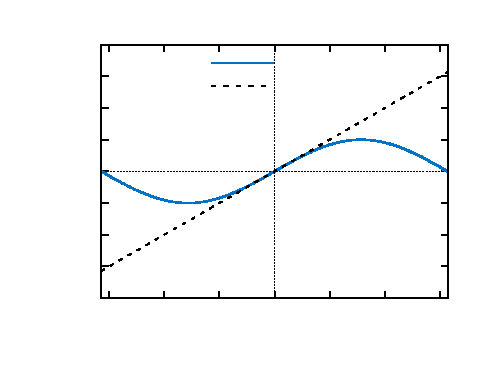
\includegraphics{sindxglobal}}%
    \gplfronttext
  \end{picture}%
\endgroup
}
 \subfloat[][]{% GNUPLOT: LaTeX picture with Postscript
\begingroup
\footnotesize
  \makeatletter
  \providecommand\color[2][]{%
    \GenericError{(gnuplot) \space\space\space\@spaces}{%
      Package color not loaded in conjunction with
      terminal option `colourtext'%
    }{See the gnuplot documentation for explanation.%
    }{Either use 'blacktext' in gnuplot or load the package
      color.sty in LaTeX.}%
    \renewcommand\color[2][]{}%
  }%
  \providecommand\includegraphics[2][]{%
    \GenericError{(gnuplot) \space\space\space\@spaces}{%
      Package graphicx or graphics not loaded%
    }{See the gnuplot documentation for explanation.%
    }{The gnuplot epslatex terminal needs graphicx.sty or graphics.sty.}%
    \renewcommand\includegraphics[2][]{}%
  }%
  \providecommand\rotatebox[2]{#2}%
  \@ifundefined{ifGPcolor}{%
    \newif\ifGPcolor
    \GPcolortrue
  }{}%
  \@ifundefined{ifGPblacktext}{%
    \newif\ifGPblacktext
    \GPblacktexttrue
  }{}%
  % define a \g@addto@macro without @ in the name:
  \let\gplgaddtomacro\g@addto@macro
  % define empty templates for all commands taking text:
  \gdef\gplbacktext{}%
  \gdef\gplfronttext{}%
  \makeatother
  \ifGPblacktext
    % no textcolor at all
    \def\colorrgb#1{}%
    \def\colorgray#1{}%
  \else
    % gray or color?
    \ifGPcolor
      \def\colorrgb#1{\color[rgb]{#1}}%
      \def\colorgray#1{\color[gray]{#1}}%
      \expandafter\def\csname LTw\endcsname{\color{white}}%
      \expandafter\def\csname LTb\endcsname{\color{black}}%
      \expandafter\def\csname LTa\endcsname{\color{black}}%
      \expandafter\def\csname LT0\endcsname{\color[rgb]{1,0,0}}%
      \expandafter\def\csname LT1\endcsname{\color[rgb]{0,1,0}}%
      \expandafter\def\csname LT2\endcsname{\color[rgb]{0,0,1}}%
      \expandafter\def\csname LT3\endcsname{\color[rgb]{1,0,1}}%
      \expandafter\def\csname LT4\endcsname{\color[rgb]{0,1,1}}%
      \expandafter\def\csname LT5\endcsname{\color[rgb]{1,1,0}}%
      \expandafter\def\csname LT6\endcsname{\color[rgb]{0,0,0}}%
      \expandafter\def\csname LT7\endcsname{\color[rgb]{1,0.3,0}}%
      \expandafter\def\csname LT8\endcsname{\color[rgb]{0.5,0.5,0.5}}%
    \else
      % gray
      \def\colorrgb#1{\color{black}}%
      \def\colorgray#1{\color[gray]{#1}}%
      \expandafter\def\csname LTw\endcsname{\color{white}}%
      \expandafter\def\csname LTb\endcsname{\color{black}}%
      \expandafter\def\csname LTa\endcsname{\color{black}}%
      \expandafter\def\csname LT0\endcsname{\color{black}}%
      \expandafter\def\csname LT1\endcsname{\color{black}}%
      \expandafter\def\csname LT2\endcsname{\color{black}}%
      \expandafter\def\csname LT3\endcsname{\color{black}}%
      \expandafter\def\csname LT4\endcsname{\color{black}}%
      \expandafter\def\csname LT5\endcsname{\color{black}}%
      \expandafter\def\csname LT6\endcsname{\color{black}}%
      \expandafter\def\csname LT7\endcsname{\color{black}}%
      \expandafter\def\csname LT8\endcsname{\color{black}}%
    \fi
  \fi
  \setlength{\unitlength}{0.0500bp}%
  \begin{picture}(4422.00,3400.00)%
    \gplgaddtomacro\gplbacktext{%
      \csname LTb\endcsname%
      \put(946,704){\makebox(0,0)[r]{\strut{}-0.3}}%
      \put(946,1109){\makebox(0,0)[r]{\strut{}-0.2}}%
      \put(946,1514){\makebox(0,0)[r]{\strut{}-0.1}}%
      \put(946,1920){\makebox(0,0)[r]{\strut{} 0}}%
      \put(946,2325){\makebox(0,0)[r]{\strut{} 0.1}}%
      \put(946,2730){\makebox(0,0)[r]{\strut{} 0.2}}%
      \put(946,3135){\makebox(0,0)[r]{\strut{} 0.3}}%
      \put(1078,484){\makebox(0,0){\strut{}-0.3}}%
      \put(1569,484){\makebox(0,0){\strut{}-0.2}}%
      \put(2060,484){\makebox(0,0){\strut{}-0.1}}%
      \put(2552,484){\makebox(0,0){\strut{} 0}}%
      \put(3043,484){\makebox(0,0){\strut{} 0.1}}%
      \put(3534,484){\makebox(0,0){\strut{} 0.2}}%
      \put(4025,484){\makebox(0,0){\strut{} 0.3}}%
      \csname LTb\endcsname%
      \put(176,1919){\rotatebox{-270}{\makebox(0,0){\strut{}$y$}}}%
      \put(2551,154){\makebox(0,0){\strut{}$x$}}%
    }%
    \gplgaddtomacro\gplfronttext{%
      \csname LTb\endcsname%
      \put(2002,2962){\makebox(0,0)[r]{\strut{}$\sin(x)$}}%
      \csname LTb\endcsname%
      \put(2002,2742){\makebox(0,0)[r]{\strut{}$x$}}%
    }%
    \gplbacktext
    \put(0,0){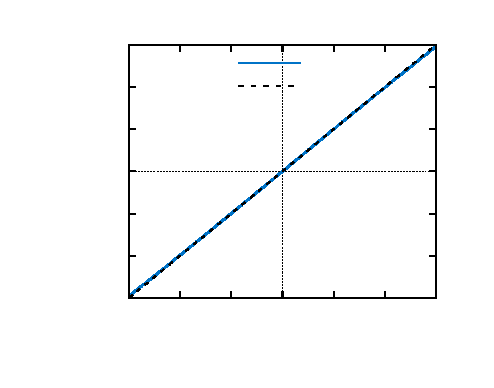
\includegraphics{sindxlocal}}%
    \gplfronttext
  \end{picture}%
\endgroup
}
 \caption[]{\quad $\sin\,\dx = \dx$: Comparing $y=\sin\,x$ and $y=x$ near $x=0$}
 \label{fig:sindx}
\end{figure}

Figure \ref{fig:sindx}(b) shows that there is virtually no difference in the
graphs even over the non-infinitesimal interval
$\ival{-0.3}{0.3}$. So $\sin\,x \approx x$ is a good approximation
when $x$ is close to 0, that is, when $\abs{x} \ll 1$ (the symbol $\ll$ means
``much less than'').\index{$\ll$} This approximation is used in many applications
in engineering and physics when the angle $x$ is assumed to be small.

Notice something else suggested by the relation $\sin\,\dx = \dx$: there is
a fundamental difference at the infinitesimal level between a line of slope 1
($y=x$) and a line of slope 0 ($y=0$). In a \emph{real} interval $(-a,a)$ around
$x=0$ the difference between the two lines can be made as small as desired by
choosing $a>0$ small enough. But in an infinitesimal interval $(-\delta,\delta)$
around $x=0$ there is unbridgeable gulf between the two lines. This is the
crucial difference in $\sin\,\dx$ being equal to $\dx$ rather than 0.

Notice also that the value of a function at an infinitesimal may itself be an
infinitesimal (e.g. $\sin\,\dx = \dx$) or a real number (e.g. $\cos\,\dx = 1$).

For a differentiable function $f(x)$, $\dfdx = f'(x)$ and so multiplying both
sides by $\dx$ yields the important relation:
\statethm{thm:df}{\vspace{-5mm}\begin{center}
 \begin{equation}\label{eqn:dffprimedx}
 \df ~=~ f'(x)\;\dx
 \end{equation}
\end{center}}
Note that both sides of the above equation are infinitesimals for each value of
$x$ in the domain of $f'$, since $f'(x)$ would then be a real number.

The notion of an infinitesimal was fairly radical at the time (and still is).
Some mathematicians embraced it, e.g. the outstanding Swiss
mathematician Leonhard Euler (1707-1783), who produced a large amount of work
using infinitesimals. But it was \emph{too} radical for
many mathematicians (and philosophers\footnote{The English philosopher George
Berkeley (1685-1753) famously derided infinitesimals as ``the ghosts of departed
quantities'' in his book \emph{The Analyst} (1734), which had the disquieting
subtitle ``A Discourse Addressed to an Infidel Mathematician'' (directed at
Newton).}), enough so
that by the 19\textsuperscript{th} century some mathematicians (notably Augustin
Cauchy and Karl Weierstrass) felt the need to put calculus on what they
considered a more ``rigorous'' footing, based on limits.\footnote{However, the
limit approach turns out, ultimately, to be equivalent to the infinitesimal
approach. In essence, only the terminology is different.}
Yet it was precisely the notion of an infinitesimal which lent calculus
its \emph{modern} character, by showing the power and usefulness of such an
abstraction (especially one that did not obey the rules of classical
mathematics).\vspace{3mm}

\divider
\vspace{3mm}
\startexercises\label{sec1dot3}
{\small
\probs{A}
\par\noindent For Exercises 1-9, let $\dx$ be an infinitesimal and prove the given formula.
\begin{enumerate}[\bfseries 1.]
\begin{multicols}{3}
 \item $(\dx \;+\; 1)^2 ~=~ 2\dx \;+\; 1$
 \item $(\dx \;+\; 1)^3 ~=~ 3\dx \;+\; 1$
 \item\label{exer:1over1plusdx} $(\dx \;+\; 1)^{-1} ~=~ 1 \;-\; \dx$
\end{multicols}
\begin{multicols}{3}
 \item $\tan\,\dx ~=~ \dx$
 \item $\sin\,2\dx ~=~ 2\dx$
 \item $\cos\,2\dx ~=~ 1$
\end{multicols}
\begin{multicols}{3}
 \item $\sin\,3\dx ~=~ 3\dx$
 \item $\cos\,3\dx ~=~ 1$
 \item $\sin\,4\dx ~=~ 4\dx$
\end{multicols}
 \item Is $\cot\,\dx$ defined for an infinitesimal $\dx$? If so, then find its value.
  If not, then explain why.
 \item In the proof of the derivative formulas for $\sin\, x$ and $\cos\, x$,
 the equation $\cos^2\,\dx = 1$ was solved to give $\cos\,\dx\ = 1$.
 Why was the other possible solution $\cos\,\dx\ = -1$ ignored?
\suspend{enumerate}
\probs{B}
\resume{enumerate}[{[\bfseries 1.]}]
 \item Show that $\ddx \,(\cos\,x) ~=~ -\sin\,x$.
 \item Show that $\ddx \,(\cos\,2x) ~=~ -2\,\sin\,2x$. \emph{(Hint: Use Exercises
 5 and 6.)}
\suspend{enumerate}
\probs{C}
\resume{enumerate}[{[\bfseries 1.]}]
 \item Show that $\ddx \,(\tan\,x) ~=~ \sec^2 \,x$. \emph{(Hint: Use Exercise 4.)}
\end{enumerate}}
\newpage
%Begin Section 1.4
\section{Derivatives of Sums, Products and Quotients}
So far the derivatives of only a few simple functions have been calculated. The
following rules will make it easier to calculate derivatives of more functions:
\index{Sum Rule}\index{Difference Rule}\index{Constant Multiple Rule}
\index{Product Rule}\index{Quotient Rule}
\index{derivative!Sum Rule}\index{derivative!Difference Rule}\index{derivative!Constant Multiple Rule}
\index{derivative!Product Rule}\index{derivative!Quotient Rule}

\statethm{thm:derivrules}{{\textbf{Rules for Derivatives:}
Suppose that $f$ and $g$ are differentiable functions of $x$. Then:
\begin{flalign*}
 \textbf{Sum Rule:}& \quad \ddx\,(f + g) ~=~ \dfdx ~+~ \dgdx &&\\[8pt]
 \textbf{Difference Rule:}& \quad \ddx\,(f - g) ~=~ \dfdx ~-~ \dgdx &&\\[8pt]
 \textbf{Constant Multiple Rule:}& \quad \ddx\,(cf) ~=~ c \cdot \dfdx \quad\text{for any constant $c$} &&\\[8pt]
 \textbf{Product Rule:}& \quad \ddx\,(f \cdot g) ~=~ f \cdot \dgdx ~+~ g \cdot \dfdx &&\\[8pt]
 \textbf{Quotient Rule:}& \quad \ddx\,\left(\dfrac{f}{g}\right) ~=~
  \dfrac{g \cdot \dfdx ~-~ f \cdot \dgdx}{g^2} &&
\end{flalign*}}}
The above rules can be written using the prime notation for derivatives:
\statethm{thm:derivrulesprime}{\vspace{-5mm}\begin{flalign*}
 \textbf{Sum Rule:}& \quad (f+g)'(x) ~=~ f'(x) ~+~ g'(x) &&\\[4pt]
 \textbf{Difference Rule:}& \quad (f-g)'(x) ~=~ f'(x) ~-~ g'(x) &&\\[4pt]
 \textbf{Constant Multiple Rule:}& \quad (cf)'(x) ~=~ c \cdot f'(x) \quad\text{for any constant $c$} &&\\[4pt]
 \textbf{Product Rule:}& \quad (f \cdot g)'(x) ~=~ f(x) \cdot g'(x) ~+~  g(x) \cdot f'(x) &&\\[4pt]
 \textbf{Quotient Rule:}& \quad \left(\dfrac{f}{g}\right)'(x) ~=~
  \dfrac{g(x) \cdot f'(x) ~-~ f(x) \cdot g'(x)}{(g(x))^2} &&
\end{flalign*}}
The proof of the Sum Rule is straightforward. Since $\dfdx$ and $\dgdx$ both exist then:
\begin{align*}
 \ddx\,(f + g) ~&=~ \dfrac{(f + g)(x + \dx) ~-~ (f + g)(x)}{\dx} ~=~
  \dfrac{f(x + \dx) ~+~ g(x + \dx) ~-~ (f(x) ~+~ g(x))}{\dx}\\[6pt]
 &=~ \dfrac{f(x + \dx) ~-~ f(x) ~+~ g(x + \dx) ~-~ g(x)}{\dx} ~=~
  \dfrac{f(x + \dx) ~-~ f(x)}{\dx} ~+~ \dfrac{g(x + \dx) ~-~ g(x)}{\dx}\\[6pt]
 &=~ \dfdx ~+~ \dgdx  \qquad \checkmark
\end{align*}
The proofs of the Difference and Constant Multiple Rules are similar and are
left as exercises.

Note that by the Product Rule, in general the derivative of a product is
\textbf{not} the product of the derivatives. That is,
$\frac{d(f \cdot g)}{\dx} \ne \dfdx \cdot \dgdx$.
This should be obvious from some earlier examples. For instance, if
$f(x) = x$ and $g(x) = 1$
then $(f \cdot g)(x) = x \cdot 1 = x$ so that $\frac{d(f \cdot g)}{\dx} = 1$,
but $\dfdx \cdot \dgdx = 1 \cdot 0 = 0$.

There is a proof of the Product Rule similar to the proof of the Sum Rule (see
Exercise 20), but there is a more geometric way of seeing why the formula holds,
described below.

\parpic[r]{\begin{tikzpicture}[>=latex,every node/.style={font=\small}]
 \draw[|<->|] (0,3.3) -- (5,3.3);
 \node[fill=white] at (2.5,3.3) {$g(x + \dx)$};
 \draw[|<->|] (5.3,3) -- (5.3,0);
 \node[fill=white,rotate=-90] at (5.3,1.5) {$f(x + \dx)$};
 \filldraw[fill=black!30,line width=1pt] (0,0) rectangle (5,3);
 \filldraw[fill=white,line width=1pt] (0,0) rectangle (4.5,2.5);
 \draw[line width=1pt] (4.5,3) -- (4.5,2.5) -- (5,2.5);
 \node[left] at (0,1.25) {$f(x)$};
 \node[left] at (0,2.75) {$\df$};
 \node[below] at (2.25,0) {$g(x)$};
 \node[below] at (4.75,0) {$\dg$};
\end{tikzpicture}}
Construct a rectangle whose perpendicular sides have lengths $f(x)$ and $g(x)$
for some $x$, as in the drawing on the right. Change $x$ by some
infinitesimal amount $\dx$, which produces infinitesimal changes $\df$ and $\dg$
in $f(x)$ and $g(x)$, respectively. Assume those changes are positive and extend
the original rectangle by those amounts, creating a larger rectangle with
perpendicular sides $f(x + \dx)$ and $g(x + \dx)$. Then
\begin{align*}
d(f \cdot g) ~&=~ (f \cdot g)(x + \dx) ~-~ (f \cdot g)(x)\\
&=~ f(x + \dx) \cdot g(x + \dx) ~-~ f(x) \cdot g(x) &\\
&=~ \text{(area of outer rectangle)} ~-~ \text{(area of original rectangle)}\\
&=~ \text{sum of the areas of the three shaded inner rectangles}\\
&=~ f(x) \cdot \dg ~+~ g(x) \cdot \df ~+~ \df \cdot \dg\\
&=~ f(x) \cdot \dg ~+~ g(x) \cdot \df ~+~ (f'(x)\;\dx) \cdot (g'(x)\;\dx)\\
&=~ f(x) \cdot \dg ~+~ g(x) \cdot \df ~+~ (f'(x) g'(x)) \cdot (\dx)^2\\
&=~ f(x) \cdot \dg ~+~ g(x) \cdot \df ~+~ (f'(x) g'(x)) \cdot 0\\
d(f \cdot g) ~&=~  f(x) \cdot \dg ~+~ g(x) \cdot \df \quad\text{, so dividing both sides by $\dx$ yields}\\[6pt]
\frac{d(f \cdot g)}{\dx} ~&=~ f(x) \cdot \dgdx ~+~ g(x) \cdot \dfdx \quad \checkmark
\end{align*}
\picskip{0}

To prove the Quotient Rule, let $y = \frac{f}{g}$, so $f = g \cdot y$. If $y$
were a differentiable function of $x$, then the Product Rule would give
\begin{gather*}
 \dfdx ~=~ \frac{d(g \cdot y)}{\dx} ~=~ g \cdot \dydx ~+~ y \cdot \dgdx ~=~
  g \cdot \dydx ~+~ \frac{f}{g} \cdot \dgdx \quad\Rightarrow\quad
  g \cdot \dydx ~=~ \dfdx ~-~ \frac{f}{g} \cdot \dgdx\\[4pt]
 \intertext{and so dividing both sides by $g$ and getting a common denominator gives}
 \dydx ~=~ \frac{1}{g} \cdot \dfdx ~-~ \frac{f}{g^2} \cdot \dgdx ~=~
  \dfrac{g \cdot \dfdx ~-~ f \cdot \dgdx}{g^2} \quad\checkmark
\end{gather*}
A simple mnemonic device for remembering the Quotient Rule is: write
$\frac{f}{g}$ as $\frac{\text{HI}}{\text{HO}}$---so that HI represents the
``high'' (numerator) part of the quotient and HO represents the ``low''
(denominator) part---and think of $d$HI and $d$HO as the derivatives of HI and
HO, respectively. Then $\ddx\left(\frac{f}{g}\right) ~=~
\frac{\text{HO} \cdot d\text{HI} ~-~ \text{HI} \cdot d\text{HO}}{\text{HO}^2}$,
pronounced as ``ho-dee-hi minus hi-dee-ho over ho-ho.''

\begin{exmp}\label{exmp:derivtan}
 Use the Quotient Rule to show that $\ddx\,(\tan\,x) = \sec^2 x$.\vspace{1mm}
 \par\noindent\emph{Solution:} Since $\tan\,x = \frac{\sin\,x}{\cos\,x}$ then:
 \begin{align*}
  \ddx\,(\tan\,x) ~&=~ \ddx\,\left(\frac{\sin\,x}{\cos\,x}\right) ~=~
   \frac{(\cos\,x) \cdot \ddx\,(\sin\,x) ~-~ (\sin\,x) \cdot \ddx\,(\cos\,x)}{\cos^2 x} ~=~
   \frac{(\cos\,x) \cdot (\cos\,x) ~-~ (\sin\,x) \cdot (-\sin\,x)}{\cos^2 x}\\[4pt]
   &=~ \frac{\cos^2 x ~+~ \sin^2 x}{\cos^2 x} ~=~ \frac{1}{\cos^2 x} ~=~ \sec^2 x
 \end{align*}
\end{exmp}
\begin{exmp}\label{exmp:derivsec}
 Use the Quotient Rule to show that $\ddx\,(\sec\,x) = \sec\,x \; \tan\,x$.\vspace{1mm}
 \par\noindent\emph{Solution:} Since $\sec\,x = \frac{1}{\cos\,x}$ then:
 \begin{align*}
  \ddx\,(\sec\,x) ~&=~ \ddx\,\left(\frac{1}{\cos\,x}\right) ~=~
   \frac{(\cos\,x) \cdot \ddx\,(1) ~-~ 1 \cdot \ddx\,(\cos\,x)}{\cos^2 x} ~=~
   \frac{(\cos\,x) \cdot 0 ~-~ 1 \cdot (-\sin\,x)}{\cos^2 x}\\[4pt]
   &=~ \frac{\sin\,x}{\cos^2 x} ~=~ \frac{1}{\cos\,x} \cdot \frac{\sin\,x}{\cos\,x} ~=~ \sec\,x \; \tan\,x
 \end{align*}
\end{exmp}
\divider
\vspace{2mm}

Similar to the above examples, the derivatives of $\cot\,x$ and $\csc\,x$ can be
found using the Quotient Rule\index{derivative!trigonometric functions} (left as
exercises)\index{trigonometric functions}. The derivatives of all
six trigonometric functions are:

\statethm{thm:trig}{\vspace{-5mm}\begin{center}
 \begin{alignat*}{3}
  \ddx\,(\cos\,x) ~&=~ -\sin\,x \qquad\qquad\qquad& \ddx\,(\sec\,x) ~&=~ \sec\,x \; \tan\,x\\[6pt]
  \ddx\,(\sin\,x) ~&=~ \cos\,x \qquad\qquad\qquad& \ddx\,(\csc\,x) ~&=~ -\csc\,x \; \cot\,x\\[6pt]
  \ddx\,(\tan\,x) ~&=~ \sec^2 x \qquad\qquad\qquad\qquad& \ddx\,(\cot\,x) ~&=~ -\csc^2 x
 \end{alignat*}
\end{center}}

Note that the Sum and Difference Rules can be applied to sums and differences,
respectively, of not just two functions but any finite (integer) number of
functions. For example, for three differentiable functions $f_1$, $f_2$, and
$f_3$,
\begin{align*}
 \ddx\,(f_1 + f_2 + f_3) ~&=~ \frac{\df_1}{\dx} ~+~ \ddx\,(f_2 + f_3) \quad\text{by the Sum Rule}\\[4pt]
 &=~ \frac{\df_1}{\dx} ~+~ \frac{\df_2}{\dx} ~+~ \frac{\df_3}{\dx} \quad\text{by the Sum Rule again.}
\end{align*}
Continuing like this for four functions, then five functions, and so forth, the
Sum and Difference Rules combined with the Constant Multiple Rule yield the
following formula:

\statethm{thm:nsum}{For $n \ge 1$ differentiable functions $f_1$, $\ldots$, $f_n$ and
constants $c_1$, $\ldots$, $c_n$:
\begin{equation}
 \ddx\,\left(c_1 f_1 ~+~ \cdots ~+~ c_n f_n\right) ~=~
 c_1 \frac{\df_1}{\dx} ~+~ \cdots ~+~ c_n \frac{\df_n}{\dx}
\end{equation}}
Note that the above formula includes differences, by using negative
constants. The formula also shows that differentiation is a
\emph{linear operation}, which makes $\ddx$ a
\emph{linear operator}\index{linear operator}. The idea is that $\ddx$
``operates'' on differentiable functions by taking their derivatives with
respect to the variable $x$. The sum $c_1 f_1 ~+~ \cdots ~+~ c_n f_n$ is called
a \emph{linear combination} of functions, and the derivative of that linear
combination can be taken term by term, with the constant multiples taken outside
the derivatives.\index{linear combination}

A special case of the above formula is replacing the functions $f_1$, $\ldots$,
$f_n$ by nonnegative powers of $x$, making the sum a polynomial in $x$. In
previous sections the derivatives of a few polynomials---such as $x$ and
$x^2$---were calculated. For the derivative of a general
polynomial\index{derivative!Power Rule}\index{Power Rule}, the following rule is
needed:
\statethm{thm:powerrule}{
\begin{displaymath}
 \textbf{Power Rule:} \quad \ddx\,\left(x^n\right) ~=~ n\,x^{n-1} \quad\text{for any integer $n$}
\end{displaymath}}
There are several ways to prove this formula; one such way being a \textbf{proof
by induction}\index{induction}\index{proof by induction}, which in general means
using the following principle:\footnote{As Bertrand Russell noted, the name is
really a misnomer: it is actually a \emph{definition} of the natural numbers
rather than a principle, and induction technically has a different meaning.}

\statethm{thm:ind}{\textbf{Principle of Mathematical Induction}\\A statement $P(n)$
about integers $n \ge k$ is true for all $n \ge k$ if:
\begin{enumerate}
 \item $P(k)$ is true.
 \item If $P(n)$ is true for some integer $n \ge k$ then $P(n+1)$ is true.
\end{enumerate}}

The idea behind mathematical induction is simple: if a statement is true about
some initial integer $k$ (Step 1 above) and if the statement being true for
\emph{some} integer implies it is true for the \emph{next} integer (Step 2 above),
then the statement being true for $k$ implies it is true for $k+1$, which in turn
implies it is true for $k+2$, which implies it is true for $k+3$, and so forth,
making it true for \emph{all} integers $n \ge k$.

Typically the initial integer $k$ will be 0 or 1. To prove the Power Rule for
all integers, first use induction to prove the rule for all nonnegative integers
$n \ge 0$, using $k = 0$ for the initial integer. For the proof by induction,
let $P(n)$ be the statement: $\ddx\,\left(x^n\right) ~=~ n\,x^{n-1}$.
\begin{enumerate}
 \item Show that $P(0)$ is true.\\That means showing that the Power
  Rule holds for $n = 0$, i.e. $\ddx\,\left(x^0\right) ~=~ 0\,x^{0-1} = 0$.
  But $x^0 = 1$ is a constant, so its derivative is 0. $\checkmark$
 \item Assuming $P(n)$ is true for some $n \ge 0$, show that $P(n+1)$ is true.\\Assuming
 that $\ddx\,\left(x^n\right) ~=~ n\,x^{n-1}$, show that
 $\ddx\,\left(x^{n+1}\right) ~=~ (n + 1)\,x^{(n+1)-1} ~=~ (n + 1)\,x^n$. It was
 shown in Section 1.2 that $\ddx\,(x) = 1$, so:
 \begin{align*}
  \ddx\,\left(x^{n+1}\right) ~&=~ \ddx\,\left( x \cdot x^n \right)\\[4pt]
  &=~ x \cdot \ddx\,\left(x^n\right) ~+~ x^n \cdot \ddx\,\left(x\right) \quad\text{(by the Product Rule)}\\[4pt]
  &=~ x \cdot n\,x^{n-1} ~+~ x^n \cdot 1 \quad\text{(by the assumption that $P(n)$ is true)}\\[4pt]
  &=~ n\,x^n ~+~ x^n ~=~ (n + 1)\,x^n \quad\checkmark
 \end{align*}
\end{enumerate}\vspace{-5mm}
\noindent Thus, by induction, the Power Rule is true for all nonnegative
integers $n \ge 0$.

To show that the Power Rule is true for all negative integers $n < 0$, write
$n = -m$, where $m$ is positive (namely, $m = \abs{n}$). Then:
\begin{align*}
 \ddx\,\left(x^n\right) ~&=~ \ddx\,\left(x^{-m}\right) ~=~ \ddx\,\left(\frac{1}{x^m}\right) ~=~
  \frac{x^m \cdot \ddx\,(1) ~-~ 1 \cdot \ddx\,\left(x^m\right)}{\left(x^m\right)^2}
  \quad\text{(by the Quotient Rule)}\\[4pt]
 &=~ \frac{x^m \cdot 0 ~-~ 1 \cdot m\,x^{m-1}}{x^{2m}} \quad\text{(by the Power Rule for positive integers)}\\[4pt]
 &=~ -m\,x^{m-1-2m} ~=~ -m\,x^{-m-1} ~=~ n\,x^{n-1} \quad\checkmark
\end{align*}
Thus, the Power Rule is true for all integers, which completes the proof. \qedsymbol

\begin{exmp}\label{exmp:polyderiv}
 Find the derivative of $f(x) = x^4 ~-~ 4x^3 ~+~ 6x^2 ~-~ 4x ~+~ 1$.\vspace{1mm}
 \par\noindent\emph{Solution:} Differentiate the polynomial term by term and use
 the Power Rule:
 \begin{align*}
  \dfdx ~&=~ \ddx\,\left(x^4 ~-~ 4x^3 ~+~ 6x^2 ~-~ 4x ~+~ 1\right)\\[4pt]
  &=~ \ddx\,\left(x^4\right) ~-~ 4 \cdot \ddx\,\left(x^3\right) ~+~ 6 \cdot \ddx\,\left(x^2\right)
      ~-~ 4 \cdot \ddx\,\left(x\right) ~+~ \ddx\,\left(1\right)\\[4pt]
  &=~ 4x^{4-1} ~-~ 4 \cdot 3x^{3-1} ~+~ 6 \cdot 2x^{2-1} ~-~ 4 \cdot 1 ~+~ 0\\[4pt]
  &=~ 4x^3 ~-~ 12x^2 ~+~ 12x ~-~ 4
 \end{align*}
\end{exmp}
\divider
\vspace{3mm}

In general, the derivative of a polynomial of degree $n \ge 0$ is given by:
\statethm{thm:poly}{For any constants $a_0$, $\ldots$, $a_n$ with $n \ge 0$:
\begin{displaymath}
 \ddx\,\left(a_n x^n ~+~  a_{n-1} x^{n-1}\cdots ~+~ a_2 x^2 ~+~ a_1 x ~+~ a_0\right) ~=~
 n a_n x^{n-1} ~+~ (n-1)\, a_{n-1} x^{n-2} ~+~ \cdots ~+~ 2 a_2 x ~+~ a_1
\end{displaymath}}
\newpage
A way to remember the Power Rule is: bring the exponent down in front of the variable
then reduce the variable's original exponent by 1. This works even for negative exponents.

\begin{exmp}\label{exmp:polyderiv2}
 Find the derivative of $f(t) = 3t^{100} ~-~ \frac{2}{t^{100}}$.\vspace{1mm}
 \par\noindent\emph{Solution:} Differentiate term by term:
 \begin{displaymath}
  \dfdt ~=~ \ddt\,\left(3t^{100} ~-~ \frac{2}{t^{100}}\right) ~=~
             \ddt\,\left( 3t^{100} ~-~ 2t^{-100}\right)
  ~=~ 3 \cdot 100t^{99} ~-~ 2 \cdot \left(-100t^{-101}\right) ~=~ 300t^{99} ~+~ \frac{200}{t^{101}}
 \end{displaymath}
\end{exmp}
\divider
\vspace{3mm}

\startexercises\label{sec1dot4}
{\small
\probs{A}
\par\noindent For Exercises 1-14, use the rules from this section to find the
 derivative of the given function.
\begin{enumerate}[\bfseries 1.]
\begin{multicols}{2}
 \item $f(x) ~=~ x^2 ~-~ x ~-~ 1$
 \item $f(x) ~=~ x^8 ~+~ 2x^4 ~+~ 1$
\end{multicols}
\begin{multicols}{2}
 \item $f(x) ~=~ \dfrac{2x^6}{3} ~-~ \dfrac{3}{2x^6}$
 \item $f(x) ~=~ \dfrac{\sin\,x ~+~ \cos\,x}{4}\vphantom{\dfrac{2x^6}{3}}$
\end{multicols}
\begin{multicols}{2}
 \item $f(x) ~=~ x\;\sin\,x$
 \item $f(x) ~=~ x^2\;\tan\,x$
\end{multicols}
\begin{multicols}{2}
 \item $f(x) ~=~ \dfrac{\sin\,x}{x}$
 \item $f(x) ~=~ \dfrac{\sin\,x}{x^2}$
\end{multicols}
\begin{multicols}{2}
 \item $f(t) ~=~ \dfrac{2t}{1 + t^2}\vphantom{\dfrac{1 - t^2}{1 + t^2}}$
 \item $g(t) ~=~ \dfrac{1 - t^2}{1 + t^2}$
\end{multicols}
\begin{multicols}{2}
 \item $f(x) ~=~ \dfrac{ax + b}{cx + d}$ ~($a$, $b$, $c$, $d$ are constants)
 \item $F(r) ~=~ -\dfrac{G m_1 m_2}{r^2}$ ~($G$, $m_1$, $m_2$ are constants)
\end{multicols}
\begin{multicols}{2}
 \item $A(r) ~=~ \pi\,r^2\vphantom{\dfrac{4}{3}}$
 \item $V(r) ~=~ \dfrac{4}{3}\,\pi r^3$
\end{multicols}
\begin{multicols}{2}
 \item Show that $\ddx \,(\cot\,x) ~=~ -\csc^2 x$.
 \item Show that $\ddx \,(\csc\,x) ~=~ -\csc\,x \; \cot\,x$.
\end{multicols}
\suspend{enumerate}
\probs{B}
\resume{enumerate}[{[\bfseries 1.]}]
\begin{multicols}{2}
 \item Prove the Difference Rule.
 \item Prove the Constant Multiple Rule.
\end{multicols}
 \item Use the Product Rule to show that for three differentiable functions $f$,
  $g$, and $h$, the derivative of their product is
  $(fgh)' = f'gh + fg'h + fgh'$.
\suspend{enumerate}
\probs{C}
\resume{enumerate}[{[\bfseries 1.]}]
 \item Provide an alternative proof of the Product Rule for two differentiable
 functions $f$ and $g$ of $x$:
 \begin{enumerate}[\bfseries (a)]
  \item Show that $(\df)(\dg) = 0$.
  \item By definition, the derivative of the product $f \cdot g$ is
   \begin{displaymath}
    \ddx\,(f \cdot g) ~=~ \frac{f(x+\dx) \cdot g(x+\dx) ~-~ f(x) \cdot g(x)}{\dx} ~.
   \end{displaymath}
   Use that formula along with part (a) to show that
   $\ddx\,(f \cdot g) ~=~ f \cdot \dgdx ~+~ g \cdot \dfdx$.\\
   \emph{(Hint: Recall that $\df ~=~ f(x+\dx) ~-~ f(x)$.)}
 \end{enumerate}
\end{enumerate}}
\newpage
%Begin Section 1.5
\section{The Chain Rule}
From what has been discussed so far it might be tempting to think that the
derivative of a function like $\sin\,2x$ is simply
$\cos\,2x$, since the derivative of $\sin\,x$ is $\cos\,x$.
It turns out that is not correct:
\begin{align*}
 \ddx\,(\sin\,2x) ~&=~ \ddx\,(2\;\sin\,x\;\cos\,x) \quad\text{(by the double-angle formula for sine)}\\[4pt]
 &=~ 2\;\ddx\,(\sin\,x\;\cos\,x) \quad\text{(by the Constant Multiple Rule)}\\[4pt]
 &=~ 2\;\left(\sin\,x \cdot \ddx\,(\cos\,x) ~+~ \cos\,x \cdot \ddx\,(\sin\,x)\right)
     \quad\text{(by the Product Rule)}\\[4pt]
 &=~ 2\;\left(\sin\,x \cdot (-\sin\,x) ~+~ \cos\,x \cdot \cos\,x\right)\\[4pt]
 &=~ 2\;\left(\cos^2 x ~-~ \sin^2 x\right)\\[4pt]
 &=~ 2\;\cos\,2x \quad\text{(by the double-angle formula for cosine)}
\end{align*}
So the derivative of $\sin\,2x$ is $2\,\cos\,2x$, \emph{not} $\cos\,2x$.

In other words, you cannot simply replace $x$ by $2x$ in the derivative formula
for $\sin\,x$. Instead, regard $\sin\,2x$ as a \emph{composition} of
two functions: the sine function and the $2x$
function.\index{function!composition} That is, let $f(u) = \sin\,u$, where the
variable $u$ itself represents a function of another variable $x$, namely
$u(x) = 2x$. So since $f$ is a function of $u$, and $u$ is a function of $x$,
then $f$ is a function of $x$, namely: $f(x) = \sin\,2x$. Since $f$ is a
differentiable function of $u$, and $u$ is a differentiable function of $x$,
then $\dfdu$ and $\dudx$ both exist (with $\dfdu = \cos\,u$ and $\dudx = 2$),
and multiplying the derivatives shows that $f$ is a differentiable function of
$x$:
\begin{align*}
 \frac{\df}{\cancel{\du}} \cdot \frac{\cancel{\du}}{\dx} ~&=~ \dfdx
  \quad\text{since the infinitesimals $\du$ cancel, so}\\[4pt]
 (\cos\,u) \cdot 2 ~&=~ \dfdx \quad\Rightarrow\quad \dfdx ~=~ 2\;\cos\,u ~=~ 2\;\cos\,2x
\end{align*}
The above argument holds in general, and is known as the
\emph{Chain Rule}\index{derivative!Chain Rule}\index{Chain Rule}:
\statethm{thm:chainrule}{\textbf{Chain Rule:} If $f$ is a differentiable
function of $u$, and $u$ is a differentiable function of $x$, then $f$ is a
differentiable function of $x$, and its derivative with respect to $x$ is:
\begin{displaymath}
  \dfdx ~=~ \dfdu \cdot \dudx
\end{displaymath}}
Notice how simple the proof is---the infinitesimals $\du$ cancel.\footnote{Some
textbooks give dire warnings to \emph{not} think that $\du$ is an actual
quantity that can be canceled. However, you can safely ignore those warnings,
because $\du$ is just an infinitesimal and hence \emph{can} be canceled!}

The Chain Rule should make sense intuitively. For example, if $\dfdu = 4$ then
that means $f$ is increasing 4 times as fast as $u$, and if $\dudx = 3$ then $u$
is increasing 3 times as fast as $x$, so overall $f$ should be increasing
$12 = 4 \cdot 3$ times as fast as $x$, exactly as the Chain Rule says.

\begin{exmp}\label{exmp:sinx2pxp1deriv}
 Find the derivative of $f(x) = \sin\,(x^2 + x + 1)$.\vspace{1mm}
 \par\noindent\emph{Solution:} The idea is to make a \emph{substitution}
 $u = x^2 + x + 1$ so that $f(x) = \sin\,u$. By the Chain Rule,
 \begin{align*}
  \dfdx ~&=~ \dfdu \cdot \dudx\\[4pt]
  &=~ \ddu\,(\sin\,u) \;\cdot\; \ddx\,(x^2 + x + 1)\\[4pt]
  &=~ (\cos\,u) \cdot (2x + 1)\\[4pt]
  &=~ (2x + 1)\,\cos\,(x^2 + x + 1)
 \end{align*}
 after replacing $u$ by its definition as a function of $x$ in the last step;
 the final answer for the derivative should be in terms of $x$, not $u$.
\end{exmp}
\divider
\vspace{3mm}

In the Chain Rule you can think of the function in question as
the composition of an ``outer'' function $f$ and an ``inner'' function $u$;
first take the derivative of the ``outer'' function then multiply by the
derivative of the ``inner'' function. Think of the ``inner'' function as a box
into which you can put any function of $x$, and the ``outer'' function being
a function of that empty box.

For instance, for the function $f(x) = \sin\,(x^2 + x + 1)$ in the previous example,
think of the ``outer'' function as $\sin\,\Box$, where $\Box = x^2 + x + 1$ is the
``inner'' function, so that
\begin{align*}
 f(x) ~&=~ \sin\,(x^2 + x + 1)\\
 &=~ \sin\,\Box\\
 \dfdx ~&=~ \left(\cos\,\Box\right) \;\cdot\; \ddx\,\Box\\[4pt]
 &=~ \left(\cos\,\setlength{\fboxsep}{2pt}\boxed{x^2 + x + 1}\right) \;\cdot\;
     \ddx\,\setlength{\fboxsep}{2pt}\boxed{x^2 + x + 1}\\[4pt]
 &=~ (2x + 1)\,\cos\,(x^2 + x + 1)
\end{align*}

\begin{exmp}\label{exmp:chainrulepow}
 Find the derivative of $f(x) = (2x^4 - 3\cos\,x)^{10}$.\vspace{1mm}
 \par\noindent\emph{Solution:} Here the ``outer'' function is $f(\Box) = \Box^{10}$
 and the ``inner'' function is $\Box = u = 2x^4 - 3\cos\,x$:
 \begin{displaymath}
  \dfdx ~=~ \dfdu \cdot \dudx ~=~ 10\,\Box^9 \;\cdot\; \ddx\,(\Box) ~=~
             10\,(2x^4 - 3\cos\,x)^9 \;(8x^3 + 3\sin\,x)
 \end{displaymath}
\end{exmp}
\divider
\newpage
Recall that the composition $f \circ g$ of two functions $f$ and $g$ is defined
as $(f \circ g)(x) = f(g(x))$. Using prime notation the Chain Rule can be
written as: 
\statethm{thm:chainruleprime}{\textbf{Chain Rule:} If $g$ is a differentiable
function of $x$, and $f$ is a differentiable function on the range of $g$, then
$f \circ g$ is a differentiable function of $x$, and its derivative with respect
to $x$ is:
\begin{displaymath}
  (f \circ g)'(x) ~=~ f'(g(x)) \;\cdot\; g'(x)
\end{displaymath}}

Using the Chain Rule, the Power Rule can be extended to include exponents that
are rational numbers:\footnote{It will be shown in Chapter 2 how to define any
real number as an exponent. The Power Rule extends to that case as well.}
\statethm{thm:xr}{\begin{displaymath}
 \ddx\,\left(x^r\right) ~=~ r\,x^{r-1} \quad\text{for any rational number $r$}
\end{displaymath}}
% To prove this, let $y = x^r = x^{m/n} = \left(x^m\right)^{1/n}$, where $m$ and
% $n$ are integers with $n \ne 0$. Then $y^n = x^m$, so taking the derivative with
% respect to $x$ of both sides of this equation gives
To prove this, let $r = m/n$, where $m$ and $n$ are integers with $n \ne 0$.
Then $y = x^r = x^{m/n} = \left(x^m\right)^{1/n}$, so that $y^n = x^m$. Taking
the derivative with respect to $x$ of both sides of this equation gives
\begin{align*}
 \ddx\,\left(y^n\right) ~&=~ \ddx\,\left(x^m\right) \quad\text{, so evaluating the
                              left side by the Chain Rule gives}\\[4pt]
 n y^{n-1} \;\cdot\; \dydx ~&=~ m x^{m-1}\\[4pt]
 n \left(x^{m/n}\right)^{n-1} \;\cdot\; \dydx ~&=~ m x^{m-1}\\[4pt]
 \dydx ~&=~ \frac{m x^{m-1}}{n x^{m - (m/n)}} ~=~
            \frac{m}{n}\,x^{m - 1 - (m - (m/n))} ~=~ \frac{m}{n}\,x^{(m/n) - 1} ~=~
            r\,x^{r-1} \quad\checkmark
\end{align*}

\begin{exmp}\label{exmp:derivsqrtx}
 Find the derivative of $f(x) = \sqrt{x}$.\vspace{1mm}
 \par\noindent\emph{Solution:} Since $\sqrt{x} = x^{1/2}$ then by the Power
 Rule:
 \begin{displaymath}
  \dfdx ~=~ \ddx\,\left(x^{1/2}\right) ~=~ \frac{1}{2}\,x^{1/2 - 1} ~=~
            \frac{1}{2}\,x^{-1/2} ~=~
            \frac{1}{2\,\sqrt{x}}
 \end{displaymath}
\end{exmp}
\begin{exmp}\label{exmp:deriv1oversqrtx}
 Find the derivative of $f(x) = \frac{2}{3\sqrt{x}}$.\vspace{1mm}
 \par\noindent\emph{Solution:}
 \begin{displaymath}
  \dfdx ~=~ \ddx\,\left(\frac{2}{3}\,x^{-1/2}\right) ~=~
            \frac{2}{3} \cdot \frac{-1}{2}\,x^{-3/2} ~=~
            -\frac{1}{3\,x^{3/2}}
 \end{displaymath}
\end{exmp}
\divider
\vspace{3mm}
\newpage
\startexercises\label{sec1dot5}
{\small
\probs{A}
\par\noindent For Exercises 1-18, find the derivative of the given function.
\begin{enumerate}[\bfseries 1.]
\begin{multicols}{2}
 \item $f(x) ~=~ (1 ~-~ 5x)^4$
 \item $f(x) ~=~ 5\,(x^3 ~+~ x ~-~ 1)^4$
\end{multicols}
\begin{multicols}{2}
 \item $f(x) ~=~ \sqrt{1 ~-~ 2x}\vphantom{{(1-x^2)}^{\tfrac{3}{2}}}$
 \item $f(x) ~=~ (1 ~-~ x^2 )^{\tfrac{3}{2}}$
\end{multicols}
\begin{multicols}{2}
 \item $f(x) ~=~ \dfrac{\sqrt{x}}{x ~+~ 1}$
 \item $f(x) ~=~ \dfrac{\sqrt{x} ~+~ 1}{\sqrt{x} ~-~ 1}$
\end{multicols}
\begin{multicols}{2}
 \item $f(t) ~=~ \left(\dfrac{1 ~-~ t}{1 ~+~ t}\right)^4\vphantom{\left(\dfrac{x^2 ~+~ 1}{x ~-~ 1}\right)^6}$
 \item $f(x) ~=~ \left(\dfrac{x^2 ~+~ 1}{x ~-~ 1}\right)^6$
\end{multicols}
\begin{multicols}{2}
 \item $f(x) ~=~ \sin^2 x$
 \item $f(x) ~=~ \cos\,\left(\sqrt{x}\right)$
\end{multicols}
\begin{multicols}{2}
 \item $f(x) ~=~ 3 \tan\,(5x)$
 \item $f(x) ~=~ A\,\cos\,(\omega x ~+~ \phi)$ ~~($A$, $\omega$, $\phi$ are constants)
\end{multicols}
\begin{multicols}{2}
 \item $f(x) ~=~ \sec\,(x^2)\vphantom{\left(\dfrac{1}{1 - x}\right)}$
 \item $f(x) ~=~ \sin^2 \left(\dfrac{1}{1 - x}\right) ~+~ \cos^2 \left(\dfrac{1}{1 - x}\right)$
\end{multicols}
\begin{multicols}{2}
 \item $L(\beta) ~=~ \dfrac{1}{\sqrt{1 ~-~ \beta^2}}\vphantom{\left(1 ~+~ \left(\dfrac{x - l}{s}\right)^2\right)^{-1}}$
 \item $f(x) ~=~ \dfrac{1}{\pi s}\left(1 ~+~ \left(\dfrac{x - l}{s}\right)^2\right)^{-1}$
       ($s$, $l$ are constants)
\end{multicols}
\begin{multicols}{2}
 \item $f(x) ~=~ \cos\,(\cos\,x)$
 \item $f(x) ~=~ \sqrt{1 ~+~ \sqrt{x}}$
\end{multicols}
\suspend{enumerate}
\probs{B}
\resume{enumerate}[{[\bfseries 1.]}]
 \item In a certain type of electronic circuit\footnote{This is an example of a
  \emph{current-differencing negative feedback amplifier}. See pp.473-479 in
  \textsc{Schilling, D.L. and C. Belove}, \emph{Electronic Circuits: Discrete and Integrated},
  2nd ed., New York: McGraw-Hill, Inc., 1979.} the \emph{overall gain} $A_v$ is given by
  \begin{displaymath}
   A_v ~=~ \frac{A_o}{1 ~-~ T}
  \end{displaymath}
  where the \emph{loop gain} $T$ is a function of the \emph{open-loop gain} $A_o$.
  \begin{enumerate}[\bfseries (a)]
   \item Show that
    \begin{displaymath}
     \frac{d \negmedspace A_v}{d\!A_o} ~=~ \frac{1}{1 ~-~ T} ~-~ \frac{A_o}{(1 ~-~ T)^2}
                                           \frac{d \negmedspace (1 - T)}{d\!A_o} ~.
    \end{displaymath}
   \item In the case where $T$ is directly proportional to $A_o$, use part (a) to
    show that
    \begin{displaymath}
     \frac{d \negmedspace A_v}{d\!A_o} ~=~ \frac{1}{(1 ~-~ T)^2} ~.
    \end{displaymath}
    \emph{(Hint: First show that $\;A_o \cdot \frac{d \negmedspace (1 - T)}{d\!A_o} ~=~ -T$.)}
  \end{enumerate}
 \item Show that the Chain Rule can be extended to 3 functions: if $u$ is a
  differentiable function of $x$, $v$ is a differentiable function of $u$, and
  $f$ is a differentiable function of $v$, then
\begin{displaymath}
 \dfdx ~=~ \dfdv \;\cdot\; \dvdu \;\cdot\; \dudx
\end{displaymath}
so that $f$ is a differentiable function of $x$. Notice that the 3 derivatives
are linked together as in a chain (hence the name of the rule). The Chain Rule
can be extended to any finite number of functions by the above technique.
\newpage
 \item In an internal combustion engine, as a piston moves downward the connecting rod
 rotates the crank in the clockwise direction, as shown in Figure \ref{fig:crank}
below.\footnote{See pp.43-45 in \textsc{Heywood, J.B.}, \emph{Internal Combustion Engine
Fundamentals}, New York: McGraw-Hill Inc., 1988.}

 \begin{figure}[h]
 \begin{center}
  \begin{tikzpicture}[every node/.style={font=\small}]
  \draw [dashed] (0,-7.5) circle (2.5);
  \filldraw [fill=white,line width=1pt,rounded corners,rotate around={15.255:(0,0)}] (240:0.9)
   arc (240:-60:0.9) -- ([shift={(0,-5.7)}] 37.875:1.1) arc (37.875:-217.875:1.1) -- cycle;
  \filldraw [fill=white,line width=1pt,rotate around={53.13:(0,-7.5)}] (0,-6.6) -- (2.5,-6.6) arc
   (90:-90:0.9) -- (0,-8.4) arc (270:90:0.9);
  \draw[dashed] (0,0) -- (1.5,-5.5) node[black,pos=0.55,sloped,below] {connecting rod}
   node[midway,above right] {$l$};
  \draw [line width=1pt] (0,0) circle (0.6);
  \fill (0,0) circle (2pt);
  \node [above] at (0,0) {$A$};
  \draw [line width=1pt] (1.5,-5.5) circle (0.6);
  \fill (1.5,-5.5) circle (2pt);
  \node [below] at (1.5,-5.5) {$B$};
  \draw [line width=1pt] (0,-7.5) circle (0.6);
  \fill (0,-7.5) circle (2pt);
  \node [below] at (0,-7.5) {$O$};
  \draw [dashed] (0,-7.5) -- (1.5,-5.5) node[sloped,midway,below] {crank};
  \draw [dashed,latex-latex] (-2.5,-7.5) -- (-0.05,-7.5) node[pos=0.4,fill=white] {$a$};
  \draw [dashed] (0,-7.5) -- (0,0) node[pos=0.5,left] {$s$};
  \draw [dashed,-latex] (0,-6.4) arc (90:53.13:1.1);
  \node at (0.4,-6.25) {$\theta$};
  \draw [line width=1pt] (-1.3,1.2) -- (1.3,1.2) -- (1.3,-1) -- (1.7,-1) -- (1.7,2) -- (-1.7,2) --
   (-1.7,-1) -- (-1.3,-1) -- cycle;
  \node at (0,1.6) {piston};
  \pattern[pattern color=black,pattern=north east lines] (-2,2.4) -- (-1.8,2.4) -- (-1.8,-1.4)
   -- (-2,-1.4) -- cycle;
  \draw [line width=1pt] (-1.8,2.4) -- (-1.8,-1.4);
  \pattern[pattern color=black,pattern=north east lines] (2,2.4) -- (1.8,2.4) -- (1.8,-1.4)
   -- (2,-1.4) -- cycle;
  \draw [line width=1pt] (1.8,2.4) -- (1.8,-1.4);
  \draw [linecolor,line width=1.5pt,-latex] (0,2.6) -- (0,2.1);
  \draw [linecolor,line width=1.5pt,-latex] (2.7,-7.5) arc (360:330:2.7);
 \end{tikzpicture} \vspace{-5mm}
 \end{center}
 \caption[]{}
 \label{fig:crank}
\end{figure}

The point $A$ can only move vertically, causing the point $B$ to move around a circle
of radius $a$ centered at the point $O$, which is directly below the point $A$ and
does not move. As the crank rotates it makes an
angle $\theta$ with the line $\overline{OA}$. Let $l = AB$ and $s = OA$ as in
the picture. Assume that all lengths are measured in centimeters, and let the time
variable $t$ be measured in minutes.
 \begin{enumerate}[\bfseries (a)]
  \item Show that $s ~=~ a \cos\,\theta ~+~ \left(l^2 ~-~ a^2 \sin^2\theta\right)^{1/2}~$
  for $0 \le \theta \le \pi$.
  \item The \emph{mean piston speed} is $\bar{S}_p = 2LN$, where $L = 2a$ is the
   \emph{piston stroke}, and $N$ is the \emph{rotational velocity}\index{rotational velocity} of
   the crank, measured in revolutions per minute (rpm). The instantaneous piston velocity
   is $S_p = \dsdt$. Let $R = l/a$. Show that for $0 \le \theta \le \pi$,
\begin{displaymath}
 \ABS{\frac{S_p}{\bar{S}_p}} ~=~ \frac{\pi}{2}\,\sin\,\theta
 \left[1 ~+~ \frac{\cos\,\theta}{\left(R^2 - \sin^2\theta\right)^{1/2}}\right] ~~.
\end{displaymath}
 \end{enumerate}
\end{enumerate}}
\newpage
%Begin Section 1.6
\section{Higher Order Derivatives}
The derivative $f'(x)$ of a differentiable function $f(x)$ can be thought of as
a function in its own right, and if it is differentiable then its
derivative---denoted by $f''(x)$---is the
\textbf{second derivative}\index{derivative!second} of $f(x)$ (the
\textbf{first derivative}\index{derivative!first} being $f'(x)$). Likewise, the
derivative of $f''(x)$ would be the \textbf{third derivative} of $f(x)$, written
as $f'''(x)$. Continuing like this yields the fourth derivative, fifth
derivative, and so on. In general the
\textbf{$\bm{n}$-th derivative}\index{derivative!$n$-th} of $f(x)$ is
obtained by differentiating $f(x)$ a total of $n$ times. Derivatives beyond the
first are called \textbf{higher order derivatives}.\index{derivative!higher
order}\index{$f^{(n)}$}\index{$\frac{d^2y}{\dx^2}$}\index{$\frac{d^n}{\dx^n}$}

\begin{exmp}
 For $f(x) = 3x^4$ find $f''(x)$ and $f'''(x)$.\vspace{1mm}
 \par\noindent\emph{Solution:} Since $f'(x) = 12x^3$ then the second derivative
 $f''(x)$ is the derivative of $12x^3$, namely:
 \begin{displaymath}
  f''(x) ~=~ 36x^2
 \end{displaymath}
 The third derivative $f'''(x)$ is then the derivative of $36x^2$, namely:
 \begin{displaymath}
  f'''(x) ~=~ 72x
 \end{displaymath}
\end{exmp}\vspace{-2mm}
\divider
\vspace{3mm}

Since the prime notation for higher order derivatives can be cumbersome (e.g.
writing 50 prime marks for the fiftieth derivative), other notations have been
created:

\statecomment{\textbf{Notation for the second derivative of $\bm{y = f(x)}$:}
The following are all equivalent:
\begin{displaymath}
  f''(x) ~~,~~~ f^{(2)}(x) ~~,~~~ \dfrac{d^2y}{\dx^2} ~~,~~~
 \dfrac{d^2}{\dx^2}\;(f(x)) ~~,~~~  y'' ~~,~~~ y^{(2)} ~~,~~~
 \ddot{y} ~~,~~~ \ddot{f}(x) ~~,~~~ \dfrac{d^2f}{\dx^2} ~~,~~~ D^2 f(x)
\end{displaymath}
\textbf{Notation for the $\bm{n}$-th derivative of $\bm{y = f(x)}$:} The
following are all equivalent:
\begin{displaymath}
  f^{(n)}(x) ~~,~~~ \dfrac{d^ny}{\dx^n} ~~,~~~
 \dfrac{d^n}{\dx^n}\;(f(x)) ~~,~~~ y^{(n)} ~~,~~~ \dfrac{d^nf}{\dx^n} ~~,~~~ D^n f(x)
\end{displaymath}}

Notice that the parentheses around $n$ in the notation $f^{(n)}(x)$ indicate
that $n$ is not an exponent---it is the number of derivatives to take. The $n$
in the Leibniz notation $\frac{d^ny}{\dx^n}$ indicates the same thing, and in
general makes working with higher order derivatives easier:
\begin{align*}
 \frac{d^2y}{\dx^2} ~&=~ \ddx\,\left(\dydx\right)\\[4pt]
 \frac{d^3y}{\dx^3} ~&=~ \ddx\,\left(\frac{d^2y}{\dx^2}\right)
                     ~=~ \frac{d^2}{\dx^2}\,\left(\dydx\right)\\
                     &\vdots\\
 \frac{d^ny}{\dx^n} ~&=~ \ddx\,\left(\frac{d^{n-1}y}{\dx^{n-1}}\right)
                    ~=~ \frac{d^{n-1}}{\dx^{n-1}}\,\left(\dydx\right)
\end{align*}
\newpage
A natural question to ask is: what do higher order derivatives represent? Recall that
the first derivative $f'(x)$ represents the instantaneous rate of change of a function
$f(x)$ at the value $x$. So the second derivative $f''(x)$ represents the instantaneous
rate of change of the function $f'(x)$ at the value $x$. In other words, the second
derivative is a rate of change of a rate of change.

\parpic[r]{\begin{tikzpicture}[>=latex,
 every node/.style={font=\small}]
 \draw[<->,black,line width=1.5pt] (-2,0) -- (2,0) node[midway, below] {$s = 0$};
 \node[above] at (1,0) {$s > 0$}; 
 \node[above] at (-1,0) {$s < 0$}; 
 \fill (0,0) circle (2.1pt);
\end{tikzpicture}}
The most famous example of this is for motion in a straight line: let $s(t)$ be
the position of an object at time $t$ as the object moves along the line. The
motion can take two directions, e.g. forward/backward or up/down. Take one
direction to represent positive position and the other to represent negative
direction, as in the drawing on the right. The (instantaneous) velocity $v(t)$
of the object at time $t$ is $s'(t)$, i.e. the first derivative of $s(t)$. The
\textbf{acceleration}\index{acceleration} $a(t)$ of the object at time $t$ is
defined as $v'(t)$, the instantaneous rate of change of the velocity. Thus,
$a(t) = s''(t)$, i.e. acceleration is the second derivative of position. To
summarize:\index{straight line motion}

\statecomment{\vspace{-5mm}\begin{center}
\begin{align*}
 s(t) ~&=~ \text{position at time $t$}\\[4pt]
 v(t) ~&=~ \text{velocity at time $t$}\\
       &=~ \dsdt ~=~ s'(t) ~=~ \dot{s}(t)\\[6pt]
 a(t) ~&=~ \text{acceleration at time $t$}\\
       &=~ \dvdt ~=~ v'(t) ~=~ \dot{v}(t)\\[4pt]
       &=~ \ddt\,\left(\dsdt\right) ~=~ \frac{d^2s}{\dt^2} ~=~ s''(t) ~=~ \ddot{s}(t)
\end{align*}
\end{center}}

\begin{exmp}\label{exmp:accel}
 Ignoring wind and air resistance, the position $s$ of a ball thrown straight up
 with an initial velocity of 34 m/s from a starting point 2 m off the ground is
 given by $s(t) = -4.9t^2 + 34t + 2$ at time $t$ (measured in seconds) with $s$
 measured in meters.
 Find the velocity and acceleration of the ball at any time $t \ge 0$.\vspace{1mm}
 \par\noindent\emph{Solution:} The ball moves in a straight vertical line, first
 straight up then straight down until it hits the ground. Its velocity $v(t)$ is
 \begin{align*}
  v(t) ~&=~ \dsdt ~=~ -9.8t ~+~ 34 ~~\text{m/s}
 \intertext{while its acceleration $a(t)$ is}
  a(t) ~&=~ \frac{d^2s}{\dt^2} ~=~ \ddt\,\left(\dsdt\right) ~=~ \ddt\,(-9.8t ~+~ 34)
       ~=~ -9.8 ~~\text{m/s}^2\text{,}
 \end{align*}
 which is the acceleration due to the force of gravity on Earth.\\
 Note that time $t = 0$ is the time at which the ball was thrown, so that
 $v(0)$ is the initial velocity of the ball.
 Indeed, $v(0) = -9.8(0) + 34 = 34$ m/s, as expected.
\end{exmp}\vspace{-2mm}
\divider
\newpage
\parpic[r]{\begin{tikzpicture}[>=latex,every node/.style={font=\small}]
\draw[->,line width=2.5pt] (0,1) -- (0,3) node[midway, left, align=center] {$v > 0$\\$a < 0$};
\draw[->,line width=2.5pt] (0.6,3) -- (0.6,0) node[pos=0.4, right, align=center] {$v < 0$\\$a < 0$};
\node[above] at (0.3,3) {$v = 0$};
\node[above] at (0.3,3.3) {$t = 3.47$};
\draw[line width=1pt] (-1.4,0) -- (2,0) node[pos=1.0,right] {$s = 0$};
\node[left] at (0,1) {$s = 2$};
\node[left] at (0,0.7) {$t=0$};
\fill (0,1) circle(2.5pt);
\end{tikzpicture}}
Notice in Example \ref{exmp:accel} that the acceleration of the ball is not only
constant but also negative. To see why this makes sense, first consider the case
where the ball is moving upward. The ball has an initial upward velocity of 34
m/s then slows down to 0 m/s at the instant it reaches its maximum height above
the ground. So the velocity is decreasing, i.e. its rate of change---the
acceleration---is negative.

The ball reaches its maximum height above the ground when its velocity is zero,
that is, when $v(t) = -9.8t + 34 = 0$, i.e. at time $t = 34/9.8 = 3.47$ seconds
after being thrown (see the picture above).
The ball then starts moving downward and its velocity is
negative (e.g. at time $t = 4$ s the velocity is
$v(4) = -9.8(4) + 34 = -5.2$ m/s).
Recall that negative velocity indicates downward motion, while positive velocity
means the motion is upward (away from the Earth's center). So in the case where
the ball begins moving downward it goes from 0 m/s to a negative velocity, with
the ball moving faster towards the ground, which it hits with a velocity of
$-33.43$ m/s (why?). So again the velocity is decreasing, which again means that
the acceleration is negative.

Common terminology involving motion might cause some confusion with the above
discussion. For example, even though the ball's acceleration is negative as it
falls to the ground, it is common to say that the ball is \emph{accelerating} in
that situation, not \emph{decelerating} (as the ball is doing while moving
upward).\index{accelerating}\index{decelerating}\index{magnitude}\index{speed}
In general, \textbf{acceleration} is understood to mean that the
\textbf{magnitude} (i.e. the absolute value) of the velocity is increasing. That
magnitude is called the \textbf{speed} of the object. \textbf{Deceleration} means
the speed is decreasing.

The first and second derivatives of an object's position with respect to time
represent the object's velocity and acceleration, respectively. Do the
third, fourth, and other higher order derivatives have any physical meanings?
It turns out they do. The third derivative of position is called
the \textbf{jerk}\index{jerk} of the object. It represents the rate of change
of acceleration, and is often used in fields such as vehicle dynamics (e.g.
minimizing jerk to provide smoother braking). The fourth, fifth, and sixth
derivatives of position are called \textbf{snap}, \textbf{crackle}, and
\textbf{pop}, respectively.\footnote{Yes, those really are their names,
obviously inspired by a certain breakfast cereal. Snap has found some uses in
flight dynamics, e.g. minimizing snap to optimize flight paths of drones.}
\index{snap}\index{crackle}\index{pop}

The \textbf{zero-th derivative}\index{derivative!zero-th} $f^{(0)}(x)$ of a
function $f(x)$ is defined to be the function $f(x)$ itself:
$f^{(0)}(x) = f(x)$. There is a way to define \textbf{fractional derivatives},
e.g. the \emph{one-half derivative} $f^{(1/2)}(x)$, which will be discussed
in Chapter 6.

An immediate consequence of the definition of higher order derivatives is:
\statethm{thm:mnderiv}{\begin{center}$\dfrac{d^{m+n}}{\dx^{m+n}}\,(f(x)) ~=~
\dfrac{d^{m}}{\dx^{m}}\,\left(\dfrac{d^{n}}{\dx^{n}}\,(f(x))\right)\quad$ for
all integers $m \ge 0$ and $n \ge 0$.\end{center}}

Recall that the \textbf{factorial}\index{factorial} $n!$ of an integer $n > 0$
is the product of the integers from 1 to $n$:
\begin{displaymath}
 n! ~=~ 1 \cdot 2 \cdot 3 \cdot \;\cdots\; \cdot n
\end{displaymath}
For example:
\begin{alignat*}{3}
 1! ~&=~ 1 \qquad\qquad& 3! ~&=~ 1 \cdot 2 \cdot 3 ~=~ 6\\
 2! ~&=~ 1 \cdot 2 ~=~ 2 \qquad\qquad& 4! ~&=~ 1 \cdot 2 \cdot 3 \cdot 4 ~=~ 24
\end{alignat*}
By convention $0!$ is defined to be 1. The following statement can be proved
using induction:
\statethm{thm:nfact}{\begin{center}$\dfrac{d^n}{\dx^n}\,\left(x^n\right) ~=~ n!\quad$
for all integers $n \ge 0$\end{center}}
Thus,
\begin{displaymath}
 \dfrac{d^{n+1}}{\dx^{n+1}}\,\left(x^n\right) ~=~
 \ddx\,\left(\dfrac{d^n}{\dx^n}\,\left(x^n\right)\right) ~=~
 \ddx\,(n!) ~=~ 0
\end{displaymath}
for all integers $n \ge 0$, since $n!$ is a constant. Polynomials are linear
combinations of nonnegative powers of a variable (e.g. $x$), so the above
result combined with the Sum Rule and the Constant Multiple rule---which
also hold for higher-order derivatives---yields this important fact:
\statethm{thm:nplus1}{The $(n+1)$-st derivative (``$n$ plus first derivative'')
of a polynomial of degree $n$ is 0:\\
For any polynomial $p(x) = a_0 ~+~ a_1 x ~+~ a_2 x^2 ~+~ \cdots ~+~ a_n x^n$
of degree $n$, $\dfrac{d^{n+1}}{\dx^{n+1}}\,(p(x)) ~=~ 0$.}
This is the basis for the commonly-used statement that ``any polynomial
can be differentiated to 0'' by taking a sufficient number of derivatives. For
example, differentiating the polynomial $p(x) = 100x^{100} + 50x^{99}$ 101 times
would yield 0 (as would differentiating more than 101 times).\vspace{3mm}

\divider
\vspace{3mm}
\startexercises\label{sec1dot6}
{\small
\probs{A}
\par\noindent For Exercises 1-6 find the second derivative of the given function.
\begin{enumerate}[\bfseries 1.]
 \begin{multicols}{3}
  \item $f(x) ~=~ x^3 ~+~ x^2 ~+~ x ~+~ 1$
  \item $f(x) ~=~ x^2\,\sin x$
  \item $f(x) ~=~ \cos 3x$
 \end{multicols}
 \begin{multicols}{3}
  \item $f(x) ~=~ \dfrac{\sin x}{x}\vphantom{\dfrac{G m_1 m_2}{r^2}}$
  \item $f(x) ~=~ \dfrac{1}{x}\vphantom{\dfrac{G m_1 m_2}{r^2}}$
  \item $F(r) ~=~ \dfrac{G m_1 m_2}{r^2}$
 \end{multicols}
 \item Find the first five derivatives of $f(x) = \sin x$. Use those to find $f^{(100)}(x)$ and $f^{(2014)}(x)$.
 \item Find the first five derivatives of $f(x) = \cos x$. Use those to find $f^{(100)}(x)$ and $f^{(2014)}(x)$.
 \item If an object moves along a straight line such that its position
  $s(t)$ at time $t$ is directly proportional to $t$ for all $t$ (written as
  $s \propto t$), then show that the object's acceleration is always 0.
\suspend{enumerate}
\probs{B}
\resume{enumerate}[{[\bfseries 1.]}]
 \item\label{exer:dnxn} Use induction to show that
  $\frac{d^n}{\dx^n}\,\left(x^n\right) ~=~ n!~$ for all integers $n \ge 1$.
 \item Show that for all integers $n \ge m \ge 1$,
  $\frac{d^{m}}{\dx^{m}}\,\left(x^n\right) ~=~ \frac{n!}{(n - m)!}\,x^{n - m} ~$.
 \item Find the general expression for the $n$-th derivative of
  $f(x) = \frac{1}{ax + b} ~$ for all constants $a$ and $b$ ($a \ne 0$).
 \item Show that the function $y = A \cos\,(\omega t + \phi) ~+~  B \sin\,(\omega t + \phi)$
  satisfies the \emph{differential equation}\index{differential equation}
  \[
   \frac{d^2y}{\dt^2} ~+~ \omega^2 y ~=~ 0
  \]
  for all constants $A$, $B$, $\omega$, and $\phi$.
 \item If $s(t)$ represents the position at time $t$ of an object
 moving along a straight line, then show that:
\begin{alignat*}{2}
 s' ~\text{and}~ s'' ~&\text{have the same sign} \quad&&\Rightarrow\quad \text{the object is accelerating}\\
 s' ~\text{and}~ s'' ~&\text{have opposite signs} &&\Rightarrow\quad \text{the object is decelerating}
\end{alignat*}
 \item For all twice-differentiable functions $f$ and $g$, show that
  $\;(f \cdot g)'' = f'' \cdot g ~+~ 2 f' \cdot g' ~+~ f \cdot g''$.
\suspend{enumerate}
\probs{C}
\resume{enumerate}[{[\bfseries 1.]}]
 \item Recall that taking a derivative is a way of
 \emph{operating} on a function. That is, think of $\ddx$ as the
 \emph{differentiation operator} on the collection of differentiable functions,
 taking a function $f(x)$ to its derivative function $\dfdx$:
 \begin{center}
  \begin{tikzpicture}[every node/.style={minimum width=2cm,minimum height=8mm}]
   \path (0,0) node(a) [drop shadow,rounded corners,draw,fill=red!05] {$f(x)$}
        (5,0) node(b) [drop shadow,rounded corners,draw,fill=red!05] {$\dfdx$};
   \draw[-latex,thick] (node cs:name=a) -- (node cs:name=b) node[midway,above]
     {$\ddx$};
  \end{tikzpicture}
 \end{center}
  Likewise, $\frac{d^2}{d\!x^2}$ is an operator on twice-differentiable
  functions, taking a function $f(x)$ to its second derivative function
  $\frac{d^2 \negmedspace f}{d\!x^2}$:
 \begin{center}
  \begin{tikzpicture}[every node/.style={minimum width=2cm,minimum height=8mm}]
   \path (0,0) node(a) [drop shadow,rounded corners,draw,fill=red!05] {$f(x)$}
         (5,0) node(b) [drop shadow,rounded corners,draw,fill=red!05]
          {$\frac{d^2 \negmedspace f}{d\!x^2}$};
   \draw[-latex,thick] (node cs:name=a) -- (node cs:name=b) node[midway,above]
     {$\frac{d^2}{d\!x^2}$};
  \end{tikzpicture}
 \end{center}
  In general, an \emph{eigenfunction} of an operator $A$ is a function
  $\phi(x)$ such that $A(\phi(x)) ~=~ \lambda \cdot \phi(x)$, that is,
 \begin{center}
  \begin{tikzpicture}[every node/.style={minimum width=2cm,minimum height=8mm}]
   \path (0,0) node(a) [drop shadow,rounded corners,draw,fill=red!05]
     {$\phi(x)$} (5,0) node(b) [drop shadow,rounded corners,draw,fill=red!05]
     {$\lambda \cdot \phi(x)$};
   \draw[-latex,thick] (node cs:name=a) -- (node cs:name=b) node[midway,above]
     {$A$};
  \end{tikzpicture}
 \end{center}
  for all $x$ in the domain of $\phi$, for some constant $\lambda$ called the
  \emph{eigenvalue} of the eigenfunction.\index{eigenfunction}\index{eigenvalue}
  \begin{enumerate}[\bfseries (a)]
   \item Show for all constants $k$ that $\phi(x) ~=~ \cos\,kx$ is an
    eigenfunction of the $\frac{d^2}{d\!x^2}$ operator, and find its eigenvalue.
    That is, show that $\frac{d^2}{d\!x^2}(\phi(x)) = \lambda \cdot \phi(x)$ for
    some constant $\lambda$ (the eigenvalue).
   \item The \emph{wave function} $\psi$ for a particle of mass $m$ moving in a
    one-dimensional box of length $L$, given by
    \begin{displaymath}
     \psi(x) ~=~ \sqrt{\frac{2}{L}}\;\sin\,\frac{\pi x}{L} \qquad\text{for
     $~0 \;\le x \;\le L$,}
	\end{displaymath}
    is a solution (assuming zero potential energy) of the time-independent
    \emph{Schr\"{o}dinger equation}\index{Schr\"{o}dinger equation}
    \begin{displaymath}
     -\frac{h^2}{8\pi^2 m}\,\frac{d^2 \negmedspace\psi}{d\!x^2} ~=~ 
	 E\,\psi(x)
	\end{displaymath}
    where $h$ is \emph{Planck's constant}\index{Planck's constant}
    and $E$ is a constant that represents the total energy of the wave function.
    Find an expression for the constant $E$ in terms of the other constants.
    Notice that this makes $\psi(x)$ an
    eigenfunction of the $\frac{d^2}{d\!x^2}$ operator.
  \end{enumerate}
\end{enumerate}}

\chapter{Derivatives of Common Functions}
%Begin Section 2.1
\section{Inverse Functions}
The derivatives calculated in the previous chapter were mostly for polynomials
and a few trigonometric functions. This chapter will show how to find the
derivatives of other types of functions, beginning in this section with inverse
functions. The idea here is that if a function is differentiable and has
an inverse then that inverse function is also differentiable.

\piccaption[]{\label{fig:function}}\parpic[r]{\begin{tikzpicture}[every node/.style={font=\small}]
 \draw [line width=1pt] (0,0) ellipse (0.8 and 0.5);
 \fill (0,0) circle (2pt);
 \node [below] at (0,0) {$x$};
 \node [above] at (0,0.6) {Domain};
 \draw [line width=1pt] (3,0) ellipse (0.8 and 0.5);
 \fill (3,0) circle (2pt);
 \node [below] at (3,0) {$y$};
 \node [above] at (3,0.53) {Range};
 \draw [-latex,line width=1.5pt] (1,0) -- (2,0) node[midway,above] {$f$}
  node[midway,below] {$y=f(x)$};
\end{tikzpicture}}
Recall that a \textbf{function}\index{function} is a rule that assigns a single
object $y$ from one set (the \textbf{range})\index{range} to each object $x$
from another set (the \textbf{domain}).\index{domain} That rule can be written
as $y = f(x)$, where $f$ is the function (see Figure \ref{fig:function}). There
is a simple \emph{vertical rule} for determining whether a rule $y=f(x)$ is a
function: $f$ is a function if and only if every vertical line intersects the
graph of $y=f(x)$ in the $xy$-coordinate plane at most once (see
Figure \ref{fig:verticalrule}).

\begin{figure}[h]
 \centering
 \subfloat[][ $f$ is a function]{
  \begin{tikzpicture}[>=latex,every node/.style={font=\small}]
   \draw[<->,black!60,line width=1pt] (0,2) node[above] {$y$} |- (4,0) node[right] {$x$};
   \draw [linecolor,line width=1.5pt] (0.5,0.5) parabola[bend at end] (3.5,1.5);
   \node[above] at (3.5,1.5) {$y=f(x)$};
   \draw[line width=1pt] (1.5,0.5) -- (1.5,2);
  \end{tikzpicture}}
 \qquad\qquad
 \subfloat[][ $f$ is not a function]{
  \begin{tikzpicture}[>=latex,every node/.style={font=\small}]
   \draw[<->,black!60,line width=1pt] (0,2) node[above] {$y$} |- (4,0) node[right] {$x$};
   \draw [linecolor,line width=1.5pt] (0.5,1.5) parabola bend  (3.5,1) (2.5,0.5);
   \node[above] at (1.5,1.5) {$y=f(x)$};
   \draw[line width=1pt] (2.8,0.2) -- (2.8,2);
  \end{tikzpicture}}\vspace{-2mm}
 \caption[]{\quad Vertical rule for functions}
 \label{fig:verticalrule}
\end{figure}

Recall that a function $f$ is \textbf{one-to-one}\index{one-to-one} (often
written as $1-1$) if it assigns distinct values of $y$ to distinct values of
$x$. In other words, if $x_1 \ne x_2$ then $f(x_1 ) \ne f(x_2 )$. Equivalently,
$f$ is one-to-one if $f(x_1 ) = f(x_2 )$ implies $x_1 = x_2$. There is a simple
\emph{horizontal rule} for determining whether a function $y=f(x)$ is
one-to-one: $f$ is one-to-one if and only if every horizontal line intersects
the graph of $y=f(x)$ in the $xy$-coordinate plane at most once (see
Figure \ref{fig:horizontalrule}).
\newpage
\begin{figure}[h]
 \centering
 \subfloat[][ $f$ is one-to-one]{
  \begin{tikzpicture}[every node/.style={font=\small}]
   \draw[latex-latex,black!60,line width=1pt] (0,2) node[above] {$y$} |- (4,0) node[right] {$x$};
   \draw [linecolor,line width=1.5pt] (0.5,0.5) parabola[bend at end] (3.5,1.5);
   \node[above] at (3.5,1.5) {$y=f(x)$};
   \draw[line width=1pt] (0.5,1) -- (2.5,1);
  \end{tikzpicture}}
 \qquad\qquad
 \subfloat[][ $f$ is not one-to-one]{
  \begin{tikzpicture}[every node/.style={font=\small}]
   \draw[latex-latex,black!60,line width=1pt] (0,2) node[above] {$y$} |- (4,0) node[right] {$x$};
   \draw [linecolor,line width=1.5pt] (0.5,0.5) parabola bend  (2,1.5) (3.5,0.5);
   \node[above] at (2,1.5) {$y=f(x)$};
   \draw[line width=1pt] (0.5,1) -- (3.5,1);
  \end{tikzpicture}}\vspace{-2mm}
 \caption[]{\quad Horizontal rule for one-to-one functions}
 \label{fig:horizontalrule}
\end{figure}

If a function $f$ is one-to-one on its domain, then $f$ has an
\textbf{inverse function}, denoted by $f^{-1}$, such that $y=f(x)$ if and only
if $f^{-1}(y) = x$. The domain of $f^{-1}$ is the range of
$f$.\index{inverse function}\index{function!inverse}

The basic idea is that $f^{-1}$ ``undoes'' what $f$ does, and vice versa. In
other words,
\begin{alignat*}{3}
 f^{-1}(f(x)) ~&=~ x \quad&&\text{for all $x$ in the domain of $f$, and}\\
 f(f^{-1}(y)) ~&=~ y \quad&&\text{for all $y$ in the range of $f$.}
\end{alignat*}

Intuitively it is clear that a function is one-to-one (and hence invertible)
when it is either strictly increasing or strictly decreasing; if the function,
say, increases and then decreases (as in Figure \ref{fig:horizontalrule}(b))
then the horizontal rule would be violated around that ``turning point.'' For
differentiable functions a positive derivative means the function is increasing,
while a negative derivative means the function is decreasing (this will be
proved in Chapter 3).

However, a function can still be one-to-one even if
its derivative is zero only at isolated points (i.e. not identically zero over
an entire interval of points) and either positive everywhere else or negative
everywhere else. For example, the function $f(x) = x^3$ has derivative
$f'(x) = 3x^2$, which is zero only at the isolated point $x = 0$ and positive
for all other values of $x$. Clearly $f$ is one-to-one over the set of all real
numbers (why?) and hence it has an inverse function $x = f^{-1}(y) = \sqrt[3]{y}$
defined for all real numbers $y$ (i.e. the range of $f$).

Thus, having a derivative that is either
always positive or always negative is \emph{sufficient} for a function to be
one-to-one but not \emph{necessary}. Having a nonzero derivative is necessary,
though, for the inverse function to be differentiable.

In algebra you learned that $\frac{a}{b} = \frac{1}{\frac{b}{a}}$ for all real
numbers $a \ne 0$ and $b \ne 0$ (and hence $\frac{b}{a} \ne 0$). The same holds
true for the infinitesimals $\dy$ and $\dx$ (nonzero by definition) since they
can be treated like numbers, which immediately yields a formula for the
derivative of an inverse function:

\statethm{thm:invderiv}{\textbf{Derivative of an Inverse Function:} If $y = f(x)$
is differentiable and has an inverse function $x = f^{-1}(y)$, then $f^{-1}$ is
differentiable and its derivative is
\[
 \dxdy ~=~ \frac{1}{\dydx} \qquad\text{if $~\dydx \ne 0$.}
\]}
The inverse of a function would still exist at a point where $\dydx = 0$
but it would not be differentiable there, since its derivative would be the
undefined quantity $\frac{1}{0}$.

Since $y$ is a function of $x$, $\dydx$ will be in terms of $x$ and hence
$\frac{1}{\dydx}$ will be in terms of $x$. However, since (by invertibility)
$x$ is a function of $y$, $\dxdy$ would normally be in terms of $y$, not $x$,
so that the two sides of the equation $\dxdy = \frac{1}{\dydx}$ are not in the
same terms!
One way to handle this discrepancy is to use the formula $y = f(x)$ to solve for
$x$ in terms of $y$ then substitute that expression into $\dydx$, so that
$\dxdy = \frac{1}{\dydx}$ is now in terms of $y$. That might not always be
possible, however (e.g. try solving for $x$ in the formula $y = x \sin x$).

\begin{exmp}\label{exmp:invderiv}
 Find the inverse $f^{-1}$ of the function $f(x) = x^3$ then find the derivative
 of $f^{-1}$.\vspace{1mm}
 \par\noindent\emph{Solution:} The function $y = f(x) = x^3$ is one-to-one over
 the set of all real numbers (why?) so it has an inverse function $x = f^{-1}(y)$
 defined for all real numbers, namely $x = f^{-1}(y) = \sqrt[3]{y}$.\vspace{1mm}
 
 \par\noindent The derivative of $f^{-1}$ is
 \begin{align*}
  \dxdy ~&=~ \frac{1}{\dydx} ~=~ \frac{1}{3x^2} \quad\text{, which is in terms of $x$,
             so putting it in terms of $y$ yields}\\[6pt]
         &=~ \frac{1}{3 \left(\sqrt[3]{y}\right)^2} ~=~
		     \frac{1}{3 y^{2/3}}
 \end{align*}
 which agrees with the derivative obtained by differentiating $x = \sqrt[3]{y}$
 directly. Note that this derivative is defined for all $y$ except $y = 0$,
 which occurs when $x = \sqrt[3]{0} = 0$, i.e. at the point $(x,y) = (0,0)$.
\end{exmp}
\divider
\vspace{3mm}

Functions are often expressed in terms of $x$, so it is common to see an
inverse function also expressed in terms of $x$: writing the inverse
of $f(x) = x^3$ as $f^{-1}(x) = \sqrt[3]{x}$ (not as
$f^{-1}(y) = \sqrt[3]{y}$)), as confusing as that might be. In that case, the
idea is to switch the roles of $x$ and $y$ in the original function $y = f(x)$,
making it $x = f(y)$, and then write $y = f^{-1}(x)$ and use
\[
 \dydx ~=~ \frac{1}{\dxdy}
\]
to put the derivative of $f^{-1}$ in terms of $x$, following the same procedure
mentioned earlier.

\begin{exmp}\label{exmp:invderivalt}
 Find the inverse $f^{-1}$ of the function $f(x) = x^3$ then find the derivative
 of $f^{-1}$.\vspace{1mm}
 \par\noindent\emph{Solution:} Rewrite $y = f(x) = x^3$ as
 $x = f(y) = y^3$, so that its inverse function $y = f^{-1}(x)= \sqrt[3]{x} $
 has derivative
 \begin{align*}
  \dydx ~&=~ \frac{1}{\dxdy} ~=~ \frac{1}{3y^2} \quad\text{, which is in terms of $y$,
             so putting it in terms of $x$ yields}\\[6pt]
         &=~ \frac{1}{3 \left(\sqrt[3]{x}\right)^2} ~=~
		     \frac{1}{3 x^{2/3}}
 \end{align*}
 which agrees with the derivative obtained by differentiating $y = \sqrt[3]{x}$
 directly.
\end{exmp}
\divider
\newpage
To obtain a formula in prime notation for the derivative of an inverse function,
notice that for all $x$ in the domain of an invertible differentiable function
$f$,
\[
 f^{-1}(f(x)) ~=~ x \quad\Rightarrow\quad
 \ddx\,\left(f^{-1}(f(x))\right) ~=~ \ddx\,(x) \quad\Rightarrow\quad
 \left(f^{-1}\right)'(f(x)) \;\cdot\; f'(x) ~=~ 1
\]
by the Chain Rule, and hence:

\statethm{thm:invprime}{\vspace{-5mm}\begin{align*}
 \left(f^{-1}\right)'(f(x)) ~&=~ \frac{1}{f'(x)} \qquad\text{if $~f'(x) \ne 0$}
\intertext{Two equivalent ways to write this are:}
 \left(f^{-1}\right)'(c) ~&=~ \frac{1}{f'(a)} \qquad\text{where $c = f(a)$ and $~f'(a) \ne 0$}
\intertext{and}
 \left(f^{-1}\right)'(x) ~&=~ \frac{1}{f'(f^{-1}(x))} \qquad\text{if $~f'(f^{-1}(x)) \ne 0$}
\end{align*}}
\divider
\vspace{3mm}
\startexercises\label{sec2dot1}
{\small
\probs{A}
\par\noindent For Exercises 1-8, show that the given function $y = f(x)$ is
 one-to-one over the given interval, then find the formulas for the inverse
 function $f^{-1}$ and its derivative. Use Example \ref{exmp:invderivalt} as a
 guide, including putting $f^{-1}$ and its derivative in terms of $x$.
\begin{enumerate}[\bfseries 1.]
 \begin{multicols}{2}
  \item $f(x) = x$, for all $x$
  \item $f(x) = 3x$, for all $x$
 \end{multicols}
 \begin{multicols}{2}
  \item $f(x) = x^2$, for all $x \ge 0$
  \item $f(x) = \sqrt{x}$, for all $x \ge 0$
 \end{multicols}
 \begin{multicols}{2}
  \item $f(x) = \frac{1}{x}$, for all $x > 0$
  \item $f(x) = \frac{1}{x}$, for all $x < 0$
 \end{multicols}
 \begin{multicols}{2}
  \item $f(x) = \frac{1}{x^2}$, for all $x > 0$
  \item $f(x) = x^5$, for all $x\vphantom{\frac{1}{x^2}}$
 \end{multicols}
 \item The unit circle $x^2 + y^2 = 1$ does not define $y$ as a single function
  of $x$, since $y = \pm \sqrt{1 - x^2}$ defines two separate functions. But
  the part of the unit circle in the first quadrant, i.e. for $0 \le x \le 1$
  and $0 \le y \le 1$, does define $y = f(x) = \sqrt{1 - x^2}$ as a single
  function of $x$ that is one-to-one on the interval $\ival{0}{1}$. Find the
  formulas for its inverse function $f^{-1}$ and its derivative.
\suspend{enumerate}
\probs{B}
\resume{enumerate}[{[\bfseries 1.]}]
 \item Show that if $f$ is differentiable and invertible, and if $f^{-1}$ is
  twice-differentiable, then
  \begin{displaymath}
   \left(f^{-1}\right)''(x) ~=~ -\frac{f''(f^{-1}(x))}{\left(f'(f^{-1}(x))\right)^3} ~.
  \end{displaymath}
\end{enumerate}}
\newpage
%Begin Section 2.2
\section{Trigonometric Functions and Their Inverses}
The graphs of the six trigonometric functions are shown in Figure
\ref{fig:trigfcns}:

\begin{figure}[ht]
 \centering
 \subfloat[][ $y\;=\;\sin\,x$]{
  \begin{tikzpicture}[scale=1.2,every node/.style={font=\small}]
  \begin{scope}[shift={(0,0)},color=linecolor,line width=1.5pt,x=3cm/360]
  \pgfplothandlerlineto
  \pgfplotfunction{\x}{0,5,...,360}{\pgfpointxy{\x}{sin(\x)}}
  \pgfusepath{stroke}
  \draw[black!60,line width=1pt,-latex] (0,0) -- (400,0) node[right] {$x$};
  \draw[black!60,line width=1pt,-latex] (0,-1.2) -- (0,1.4) node[above] {$y$};
  \node[black,left] at (0,0) {$0$};
  \foreach \pos in {90,180,270,360}
   \draw[black!60,line width=0.3pt,shift={(\pos,0)}] (0pt,3pt) -- (0pt,-3pt);
  \foreach \pos in {-1,1}
   \draw[black!60,line width=0.3pt,shift={(0,\pos)}] (3pt,0pt) -- (-3pt,0pt);
  \node[black,left] at (0,1) {$1$};
  \node[black,left] at (0,-1) {$-1$};
  \node[black,below] at (90,-0.1) {$\tfrac{\pi}{2}$};
  \node[black,below] at (180,-0.1) {$\pi$};
  \node[black,below] at (270,-0.1) {$\tfrac{3\pi}{2}$};
  \node[black,below] at (368,-0.1) {$2\pi$};
 \end{scope}
\end{tikzpicture}}
 \quad
 \subfloat[][ $y\;=\;\cos\,x$]{
  \begin{tikzpicture}[scale=1.2,every node/.style={font=\small}]
  \begin{scope}[shift={(0,0)},color=linecolor,line width=1.5pt,x=3cm/360]
  \pgfplothandlerlineto
  \pgfplotfunction{\x}{0,5,...,360}{\pgfpointxy{\x}{cos(\x)}}
  \pgfusepath{stroke}
  \draw[black!60,line width=1pt,-latex] (0,0) -- (400,0) node[right] {$x$};
  \draw[black!60,line width=1pt,-latex] (0,-1.2) -- (0,1.4) node[above] {$y$};
  \node[black,left] at (0,0) {$0$};
  \foreach \pos in {90,180,270,360}
   \draw[black!60,line width=0.3pt,shift={(\pos,0)}] (0pt,3pt) -- (0pt,-3pt);
  \foreach \pos in {-1,1}
   \draw[black!60,line width=0.3pt,shift={(0,\pos)}] (3pt,0pt) -- (-3pt,0pt);
  \node[black,left] at (0,1) {$1$};
  \node[black,left] at (0,-1) {$-1$};
  \node[black,below] at (90,-0.1) {$\tfrac{\pi}{2}$};
  \node[black,below] at (180,-0.1) {$\pi$};
  \node[black,below] at (275,-0.1) {$\tfrac{3\pi}{2}$};
  \node[black,below] at (362,-0.1) {$2\pi$};
 \end{scope}
\end{tikzpicture}}
 \quad
 \subfloat[][ $y\;=\;\tan\,x$]{
  \begin{tikzpicture}[scale=1.2,every node/.style={font=\small}]
  \begin{scope}[shift={(0,0)},color=linecolor,line width=1.5pt,x=3cm/360]
  \pgfplothandlerlineto
  \pgfplotfunction{\x}{-82,-80,...,82}{\pgfpointxy{\x}{0.34*tan(0.9*\x)}}
  \pgfusepath{stroke}
  \draw[black!60,dashed,line width=0.3pt] (-90,-1.2) -- (-90,1.2);
  \draw[black!60,dashed,line width=0.3pt] (90,-1.2) -- (90,1.2);
  \draw[black!60,line width=1pt,-latex] (-130,0) -- (130,0) node[right] {$x$};
  \draw[black!60,line width=1pt,-latex] (0,-1.2) -- (0,1.4) node[above] {$y$};
  \node[black,below right] at (0,0) {$0$};
  \node[black,below left] at (-90,-0.1) {$-\tfrac{\pi}{2}$};
  \node[black,below right] at (90,-0.1) {$\tfrac{\pi}{2}$};
 \end{scope}
\end{tikzpicture}}
\\\vspace{1mm}
 \subfloat[][ $y~=~\csc\,x$]{
  \begin{tikzpicture}[scale=1.2,every node/.style={font=\small}]
  \begin{scope}[shift={(0,0)},color=linecolor,line width=1.5pt,x=3cm/360]
  \pgfplothandlerlineto
  \pgfplotfunction{\x}{8,10,...,172}{\pgfpointxy{\x}{0.5 + 0.1/sin(\x)}}
  \pgfusepath{stroke}
  \pgfplothandlerlineto
  \pgfplotfunction{\x}{188,190,...,352}{\pgfpointxy{\x}{-0.5 + 0.1/sin(\x)}}
  \pgfusepath{stroke}
  \draw[black!60,line width=1pt,-latex] (0,0) -- (400,0) node[right] {$x$};
  \draw[black!60,line width=1pt,-latex] (0,-1.2) -- (0,1.5) node[above] {$y$};
  \draw[black!60,dashed,line width=0.3pt] (180,-1.2) -- (180,1.4);
  \draw[black!60,dashed,line width=0.3pt] (360,-1.2) -- (360,1.4);
  \node[black,left] at (0,0) {$0$};
  \foreach \pos in {90,180,270,360}
   \draw[black!60,line width=0.3pt,shift={(\pos,0)}] (0pt,3pt) -- (0pt,-3pt);
  \foreach \pos in {-0.6,0.6}
   \draw[black!60,line width=0.3pt,shift={(0,\pos)}] (3pt,0pt) -- (-3pt,0pt);
  \node[black,left] at (0,0.6) {$1$};
  \node[black,left] at (0,-0.6) {$-1$};
  \node[black,below] at (90,-0.1) {$\tfrac{\pi}{2}$};
  \node[black,below] at (180,-0.1) {$\pi$};
  \node[black,below] at (270,-0.05) {$\tfrac{3\pi}{2}$};
  \node[black,below] at (368,-0.1) {$2\pi$};
 \end{scope}
\end{tikzpicture}}
 \quad
 \subfloat[][ $y~=~\sec\,x$]{
  \begin{tikzpicture}[scale=1.2,every node/.style={font=\small}]
  \begin{scope}[shift={(0,0)},color=linecolor,line width=1.5pt,x=3cm/360]
  \pgfplothandlerlineto
  \pgfplotfunction{\x}{0,2,...,82}{\pgfpointxy{\x}{0.5 + 0.1/cos(\x)}}
  \pgfusepath{stroke}
  \pgfplothandlerlineto
  \pgfplotfunction{\x}{98,100,...,262}{\pgfpointxy{\x}{-0.5 + 0.1/cos(\x)}}
  \pgfusepath{stroke}
  \pgfplothandlerlineto
  \pgfplotfunction{\x}{278,280,...,360}{\pgfpointxy{\x}{0.5 + 0.1/cos(\x)}}
  \pgfusepath{stroke}
  \draw[black!60,line width=1pt,-latex] (0,0) -- (400,0) node[right] {$x$};
  \draw[black!60,line width=1pt,-latex] (0,-1.2) -- (0,1.5) node[above] {$y$};
  \draw[black!60,dashed,line width=0.3pt] (90,-1.2) -- (90,1.4);
  \draw[black!60,dashed,line width=0.3pt] (270,-1.2) -- (270,1.4);
  \node[black,left] at (0,0) {$0$};
  \foreach \pos in {90,180,270,360}
   \draw[black!60,line width=0.3pt,shift={(\pos,0)}] (0pt,3pt) -- (0pt,-3pt);
  \foreach \pos in {-0.6,0.6}
   \draw[black!60,line width=0.3pt,shift={(0,\pos)}] (3pt,0pt) -- (-3pt,0pt);
  \node[black,left] at (0,0.6) {$1$};
  \node[black,left] at (0,-0.6) {$-1$};
  \node[black,below] at (90,-0.1) {$\tfrac{\pi}{2}$};
  \node[black,below] at (180,-0.1) {$\pi$};
  \node[black,below] at (270,-0.05) {$\tfrac{3\pi}{2}$};
  \node[black,below] at (368,-0.1) {$2\pi$};
 \end{scope}
\end{tikzpicture}}
 \quad
 \subfloat[][ $y~=~\cot\,x$]{
  \begin{tikzpicture}[scale=1.2,every node/.style={font=\small}]
  \begin{scope}[shift={(0,0)},color=linecolor,line width=1.5pt,x=3cm/360]
  \pgfplothandlerlineto
  \pgfplotfunction{\x}{8,10,...,172}{\pgfpointxy{\x}{-0.5*tan(0.8*(-90+\x))}}
  \pgfusepath{stroke}
  \draw[black!60,dashed,line width=0.3pt] (180,-1.2) -- (180,1.4);
  \draw[black!60,line width=1pt,-latex] (0,0) -- (230,0) node[right] {$x$};
  \draw[black!60,line width=1pt,-latex] (0,-1.2) -- (0,1.5) node[above] {$y$};
  \node[black,left] at (0,0) {$0$};
  \foreach \pos in {90}
   \draw[black!60,line width=0.3pt,shift={(\pos,0)}] (0pt,3pt) -- (0pt,-3pt);
  \node[black,below] at (90,-0.1) {$\tfrac{\pi}{2}$};
  \node[black,below right] at (180,-0.1) {$\pi$};
 \end{scope}
\end{tikzpicture}}\vspace{-1mm}
 \caption[]{\quad Graphs of the six trigonometric functions}
 \label{fig:trigfcns}
\end{figure}
\noindent Recall that $\sin\,x$, $\cos\,x$, $\csc\,x$, and $\sec\,x$ have a
period of $2\pi$ (i.e. repeat the same values every $2\pi$ radians), while
$\tan\,x$ and $\cot\,x$ have a period of $\pi$.\vspace{2mm}

\noindent The derivatives of the six trigonometric functions---given in Section
1.4---are:\index{trigonometric functions}\index{function!trigonometric}

\statethm{thm:trig2}{\vspace{-4mm}\begin{alignat*}{4}
 \ddx\,(\sin x) ~&=~ \cos x
 \qquad\qquad\qquad\qquad& \ddx\,(\csc x) ~&=~ -\csc x \; \cot x\\[6pt]
 \ddx\,(\cos x) ~&=~ -\sin x
 \qquad\qquad\qquad\qquad& \ddx\,(\sec x) ~&=~ \sec x \; \tan x\\[6pt]
 \ddx\,(\tan x) ~&=~ \sec^2 x
 \qquad\qquad\qquad\qquad& \ddx\,(\cot x) ~&=~ -\csc^2 x
\end{alignat*}}

The six trigonometric functions are not one-to-one over their entire domains,
but recall from trigonometry that they are one-to-one when restricted to smaller
domains, and hence have inverse functions, called the \textbf{inverse
trigonometric functions}.\index{inverse trigonometric
functions}\index{function!inverse trigonometric}\index{trigonometric
functions!inverses}
\newpage
\noindent For example, $y = \sin\,x$ is one-to-one over the interval
$\left[ -\frac{\pi}{2},\frac{\pi}{2} \right]$, as shown in
Figure \ref{fig:sinerestricted} below:

\begin{figure}[h]
 \begin{center}
  \begin{tikzpicture}[scale=1.2,every node/.style={font=\small}]
   \begin{scope}[black!60,dashed,line width=1.5pt,x=6cm/360]
	\draw[black!60,solid,line width=1pt,-latex] (-200,0) -- (220,0) node[right] {$x$};
	\draw[black!60,solid,line width=1pt,-latex] (0,-1.2) -- (0,1.5) node[above] {$y$};
	\pgfplothandlerlineto
	\pgfplotfunction{\x}{-180,-175,...,-90}{\pgfpointxy{\x}{sin(\x)}}
	\pgfusepath{stroke}
	\pgfplothandlerlineto
	\pgfplotfunction{\x}{90,95,...,180}{\pgfpointxy{\x}{sin(\x)}}
	\pgfusepath{stroke}
	\node[black,below right] at (0,0) {$0$};
	\foreach \pos in {-180,-90,90,180}
	 \draw[black!60,line width=0.3pt,solid,shift={(\pos,0)}] (0pt,3pt) -- (0pt,-3pt);
	\foreach \pos in {-1,1}
	 \draw[black!60,line width=0.3pt,solid,shift={(0,\pos)}] (3pt,0pt) -- (-3pt,0pt)
	  node[black,left] {$\pos$};
	\node[black,below] at (90,-0.1) {$\tfrac{\pi}{2}$};
	\node[black,below] at (180,-0.1) {$\pi$};
	\node[black,below] at (-90,-0.1) {$-\tfrac{\pi}{2}$};
	\node[black,below] at (-180,-0.1) {$-\pi$};
	\node[black,above] at (180,1) {$y=\sin\;x$};
   \end{scope}
   \begin{scope}[color=linecolor,line width=1.5pt,x=6cm/360]
	\pgfplothandlerlineto
	\pgfplotfunction{\x}{-90,-85,...,90}{\pgfpointxy{\x}{sin(\x)}}
	\pgfusepath{stroke}
	\fill (-90,-1) circle (2pt);
	\fill (90,1) circle (2pt);
   \end{scope}
  \end{tikzpicture}\vspace{-6mm}
 \end{center}
 \caption[]{\quad $y=\sin\,x$ is one-to-one with $x$ restricted to $\left[ -\frac{\pi}{2},\frac{\pi}{2} \right]$}
 \label{fig:sinerestricted}
\end{figure}

\noindent Similarly, recall that $\cos\,x$ is one-to-one over $\ival{0}{\pi}$,
$\tan\,x$ is one-to-one over $(-\pi/2,\pi/2)$,
$\csc\,x$ is one-to-one over $(-\pi/2,0) \cup (0,\pi/2)$,
$\sec\,x$ is one-to-one over $(0,\pi/2) \cup (\pi/2,\pi)$, and
$\cot\,x$ is one-to-one over $(0,\pi)$. Hence, the inverse trigonometric
functions $\sin^{-1} x$, $\cos^{-1} x$, $\tan^{-1} x$, $\csc^{-1} x$, $\sec^{-1} x$
and $\cot^{-1} x$ are defined,\footnote{The \emph{arc} notation $\arcsin\,x$,
$\arccos\,x$, $\arctan\,x$, $\arccsc\,x$, $\arcsec\,x$, $\arccot\,x$ is often
used in place of $\sin^{-1}x$, $\cos^{-1}x$, $\tan^{-1}x$, $\csc^{-1}x$,
$\sec^{-1}x$, $\cot^{-1}x$, respectively.} with the following domains and ranges:

\begin{center}
\bgroup
\def\arraystretch{1.5}
\begin{tabular}{@{}|r||c|c|c|c|c|c|@{}}
\hline
function & $\sin^{-1} x$ & $\cos^{-1} x$ & $\tan^{-1} x$ & $\csc^{-1} x$ & $\sec^{-1} x$ & $\cot^{-1} x$\\
\hline
domain & $\ival{-1}{1}$ & $\ival{-1}{1}$ & $(-\infty,\infty)$ & $\abs{x} \ge 1$ & $\abs{x} \ge 1$
& $(-\infty,\infty)$\\
\hline
range & $\ival{-\tfrac{\pi}{2}}{\tfrac{\pi}{2}}$ & $\ival{0}{\pi}$ &
$\left(-\tfrac{\pi}{2},\tfrac{\pi}{2}\right)$ &
$\left(-\tfrac{\pi}{2},0\right) \cup \left(0,\tfrac{\pi}{2}\right)$ &
$\left(0,\tfrac{\pi}{2}\right) \cup \left(\tfrac{\pi}{2},\pi\right)$ &
$(0,\pi)$\\
\hline
\end{tabular}
\egroup
\end{center}

\noindent The graphs of all six inverse trigonometric functions are shown in
Figures \ref{fig:invtrigfcns1} and \ref{fig:invtrigfcns2} below:

\begin{figure}[ht]
 \centering
 \subfloat[][ $y\;=\;\sin^{-1} x$]{
  \begin{tikzpicture}[scale=1.2,every node/.style={font=\small}]
   \begin{scope}[x=6cm/360]
    \draw[black!60,line width=1pt,-latex] (-70,0) -- (80,0) node[right] {$x$};
    \draw[black!60,line width=1pt,-latex] (0,-1.9) -- (0,2.1) node[above] {$y$};
    \node[black,below right] at (0,0) {$0$};
    \foreach \pos in {-60,60}
     \draw[black!60,line width=0.3pt,shift={(\pos,0)}] (0pt,3pt) -- (0pt,-3pt);
    \foreach \pos in {-1.5}
     \draw[black!60,line width=0.3pt,shift={(0,\pos)}] (3pt,0pt) -- (-3pt,0pt)
      node[black,left] {$-\tfrac{\pi}{2}$};
    \foreach \pos in {1.5}
     \draw[black!60,line width=0.3pt,shift={(0,\pos)}] (3pt,0pt) -- (-3pt,0pt)
      node[black,left] {$\tfrac{\pi}{2}$};
    \node[black,below] at (60,-0.1) {$1$};
    \node[black,below] at (-60,-0.1) {$-1$};
   \end{scope}
   \begin{scope}[color=linecolor,line width=1.5pt,x=6cm/360,cm={0,1,1,0,(0,0)}]
    \pgfplothandlerlineto
    \pgfplotfunction{\x}{-90,-85,...,90}{\pgfpointxy{\x}{sin(\x)}}
    \pgfusepath{stroke}
    \fill[black] (-90,-1) circle (2pt);
    \fill[black] (90,1) circle (2pt);
   \end{scope}
\end{tikzpicture}}
 \quad
 \subfloat[][ $y\;=\;\cos^{-1} x$]{
  \begin{tikzpicture}[scale=1.2,every node/.style={font=\small}]
   \begin{scope}[x=6cm/360]
    \draw[black!60,line width=1pt,-latex] (-70,0) -- (90,0) node[right] {$x$};
    \draw[black!60,line width=1pt,-latex] (0,-0.2) -- (0,3.5) node[above] {$y$};
    \node[black,below right] at (0,0) {$0$};
    \foreach \pos in {-60,60}
     \draw[black!60,line width=0.3pt,shift={(\pos,0)}] (0pt,3pt) -- (0pt,-3pt);
    \foreach \pos in {3}
     \draw[black!60,line width=0.3pt,shift={(0,\pos)}] (3pt,0pt) -- (-3pt,0pt)
      node[black,left] {$\pi$};
    \node[black,below] at (60,-0.1) {$1$};
    \node[black,below] at (-60,-0.1) {$-1$};
   \end{scope}
   \begin{scope}[color=linecolor,line width=1.5pt,x=6cm/360,cm={0,1,1,0,(0,0)}]
    \pgfplothandlerlineto
    \pgfplotfunction{\x}{0,5,...,180}{\pgfpointxy{\x}{cos(\x)}}
    \pgfusepath{stroke}
    \fill[black] (0,1) circle (2pt);
    \fill[black] (180,-1) circle (2pt);
   \end{scope}
\end{tikzpicture}}
\quad
 \subfloat[][ $y\;=\;\tan^{-1} x$]{
  \begin{tikzpicture}[scale=1.2,every node/.style={font=\small}]
   \begin{scope}[dashed,line width=1pt,x=6cm/360,y=3cm/6]
	\draw[black!60,solid,line width=0.3pt,-latex] (-150,0) -- (150,0) node[right] {$x$};
	\draw[black!60,solid,line width=0.3pt,-latex] (0,-4) -- (0,4) node[above] {$y$};
	\node[black,below right] at (0,0) {$0$};
	\foreach \pos in {3.14}
	 \draw[black!60,solid,line width=0.3pt,shift={(0,\pos)}] (3pt,0pt) -- (-3pt,0pt)
	  node[black,left] {$\tfrac{\pi}{2}$};
	\foreach \pos in {-3.14}
	 \draw[black!60,solid,line width=0.3pt,shift={(0,\pos)}] (3pt,0pt) -- (-3pt,0pt)
	  node[black,left] {$-\tfrac{\pi}{2}$};
	\draw[black!60,line width=0.5pt] (-150,-3.14) -- (140,-3.14);
	\draw[black!60,line width=0.5pt] (-150,3.14) -- (140,3.14);
   \end{scope}
   \begin{scope}[color=linecolor,line width=1.5pt,x=6cm/360,y=3cm/6,cm={0,1,1,0,(0,0)}]
	\pgfplothandlerlineto
	\pgfplotfunction{\x}{-78,-76,...,78}{\pgfpointxy{\x}{tan(\x)}}
	\pgfusepath{stroke}
   \end{scope}
\end{tikzpicture}}\vspace{-1mm}
 \caption[]{\quad Graphs of $\sin^{-1} x$, $\cos^{-1} x$, $\tan^{-1} x$}
 \label{fig:invtrigfcns1}
\end{figure}
\newpage
\begin{figure}[ht]
 \centering
 \subfloat[][ $y~=~\csc^{-1} x$]{
  \begin{tikzpicture}[scale=0.8,every node/.style={font=\small}]
   \begin{scope}[line width=1pt,x=4cm/360]
    \draw[black!60,solid,line width=1pt,-latex] (-230,0) -- (230,0) node[right] {$x$};
    \draw[black!60,solid,line width=1pt,-latex] (0,-2) -- (0,2.5) node[above] {$y$};
    \node[black,above left] at (0,0) {$0$};
    \foreach \pos in {-90,90}
     \draw[black!60,line width=0.3pt,shift={(\pos,0)}] (0pt,3pt) -- (0pt,-3pt);
    \foreach \pos in {1.5}
     \draw[black!60,line width=0.3pt,shift={(0,\pos)}] (-3pt,0pt) -- (3pt,0pt) node[black,left]
      {$\tfrac{\pi}{2}$};
    \foreach \pos in {-1.5}
     \draw[black!60,line width=0.3pt,shift={(0,\pos)}] (-3pt,0pt) -- (3pt,0pt) node[black,left]
      {$-\tfrac{\pi}{2}$};
    \node[black,below] at (90,-0.1) {$1$};
    \node[black,below] at (-90,-0.1) {$-1$};
   \end{scope}
   \begin{scope}[color=linecolor,line width=1.5pt,x=4cm/360,cm={0,1,1,0,(0,0)}]
    \pgfplothandlerlineto
    \pgfplotfunction{\x}{-135,-130,...,-70}{\pgfpointxy{\x}{1/sin(45+\x)}}
    \pgfplotfunction{\x}{70,75,...,135}{\pgfpointxy{\x}{1/sin(-45+\x)}}
    \pgfusepath{stroke}
    \fill[black] (135,1) circle (2.5pt);
    \fill[black] (-135,-1) circle (2.5pt);
   \end{scope}
\end{tikzpicture}}
\quad\quad
 \subfloat[][ $y~=~\sec^{-1} x$]{
  \begin{tikzpicture}[scale=0.8,every node/.style={font=\small}]
   \begin{scope}[line width=1.2pt,x=4cm/360]
    \draw[black!60,-latex] (-230,0) -- (230,0) node[right] {$x$};
    \draw[black!60,-latex] (0,0) -- (0,3.8) node[above] {$y$};
    \node[black,below] at (0,0) {$0$};
    \foreach \pos in {-90,90}
     \draw[black!60,line width=0.4pt,shift={(\pos,0)}] (0pt,3pt) -- (0pt,-3pt);
    \foreach \pos in {3}
     \draw[black!60,line width=0.4pt,shift={(0,\pos)}] (-3pt,0pt) -- (3pt,0pt) node[black,left]
      {$\pi$};
    \foreach \pos in {1.5}
     \draw[black!60,line width=0.4pt,shift={(0,\pos)}] (-3pt,0pt) -- (3pt,0pt) node[black,left]
      {$\tfrac{\pi}{2}$};
    \node[black,below] at (90,-0.1) {$1$};
    \node[black,below] at (-90,-0.1) {$-1$};
    \draw[black!60,dashed,line width=0.4] (-230,1.5) -- (230,1.5);
   \end{scope}
   \begin{scope}[color=linecolor,line width=1.5pt,x=4cm/360,cm={0,1,1,0,(0,0)}]
    \pgfplothandlerlineto
    \pgfplotfunction{\x}{0,5,...,65}{\pgfpointxy{\x}{1/cos(\x)}}
    \pgfplotfunction{\x}{205,210,...,270}{\pgfpointxy{\x}{1/cos(-90+\x)}}
    \pgfusepath{stroke}
    \fill[black] (270,-1) circle (2.5pt);
    \fill[black] (0,1) circle (2.5pt);
   \end{scope}
\end{tikzpicture}}
 \quad\quad
 \subfloat[][ $y~=~\cot^{-1} x$]{
  \begin{tikzpicture}[every node/.style={font=\small}]
   \begin{scope}[line width=1pt]
    \draw[black!60,-latex] (-2,0) -- (2,0) node[right] {$x$};
    \draw[black!60,-latex] (0,0) -- (0,3) node[above] {$y$};
    \node[black,below] at (0,0) {$0$};
    \foreach \pos in {2}
     \draw[black!60,line width=0.4pt,shift={(0,\pos)}] (-3pt,0pt) -- (3pt,0pt) node[black,above left]
      {$\pi$};
    \foreach \pos in {1}
     \draw[black!60,line width=0.4pt,shift={(0,\pos)}] (-3pt,0pt) -- (3pt,0pt) node[black,right]
      {$\tfrac{\pi}{2}$};
    \draw[black!60,dashed,line width=0.4] (-2,2) -- (2,2);
   \end{scope}
   \begin{scope}[color=linecolor,line width=1.5pt,cm={0,1,3.1,0,(0,0)}]
    \pgfplothandlerlineto
    \pgfplotfunction{\x}{10,15,...,170}{\pgfpointxy{\x/90}{-0.088*tan(90+\x)}}
    \pgfusepath{stroke}
   \end{scope}
\end{tikzpicture}}\vspace{-1mm}
 \caption[]{\quad Graphs of $\csc^{-1} x$, $\sec^{-1} x$, $\cot^{-1} x$}
 \label{fig:invtrigfcns2}
\end{figure}

\noindent The derivatives of the six inverse trigonometric functions are:

\statethm{thm:invtrig}{\vspace{-4mm}\begin{alignat*}{4}
 \ddx\,(\sin^{-1} x) ~&=~ \frac{1}{\sqrt{1 - x^2}} \quad\text{(for $\abs{x} < 1$)}
 \qquad\quad\quad& \ddx\,(\csc^{-1} x) ~&=~ -\,\frac{1}{\abs{x}\sqrt{x^2 - 1}}
 \quad\text{(for $\abs{x} > 1$)}\\[6pt]
 \ddx\,(\cos^{-1} x) ~&=~ -\,\frac{1}{\sqrt{1 - x^2}} \quad\text{(for $\abs{x} < 1$)}
 \qquad\quad\quad& \ddx\,(\sec^{-1} x) ~&=~ \frac{1}{\abs{x}\sqrt{x^2 - 1}}
 \quad\text{(for $\abs{x} > 1$)}\\[6pt]
 \ddx\,(\tan^{-1} x) ~&=~ \frac{1}{1 + x^2}
 \qquad\quad\quad& \ddx\,(\cot^{-1} x) ~&=~ -\,\frac{1}{1 + x^2}
\end{alignat*}}
For the derivative of $\cos^{-1} x$,
recall that $y = \cos^{-1} x$ is an \emph{angle} between $0$ and $\pi$ radians,
defined for $-1 \le x \le 1$. Since $\cos y = x$ by the definition of $y$, then
$\dxdy = -\sin y$ and
\begin{displaymath}
 \sin^2 y ~=~ 1 - \cos^2 y ~=~ 1 - x^2 \quad\Rightarrow\quad
 \sin y ~=~ \pm\,\sqrt{1 - x^2} ~=~ \sqrt{1 - x^2}
\end{displaymath}
since $0 \le y \le \pi$ (which means $\sin y$ must be nonnegative). Thus:
\begin{displaymath}
 \ddx\,(\cos^{-1} x) ~=~ \dydx ~=~ \frac{1}{\dxdy} ~=~ \frac{1}{-\sin y} ~=~
  -\,\frac{1}{\sqrt{1 - x^2}} \quad\checkmark
 \end{displaymath}

For the derivative of $\sec^{-1} x$, since $y = \sec^{-1} x$ is defined for
$\abs{x} \ge 1$, then  $0 \le y < \pi/2$ for $x \ge 1$ and $\pi/2 < y \le \pi$
for $x \le -1$. Recall also that $\sec y$ and $\tan y$ are both positive  when
$0 < y < \pi/2$ and are both negative when $\pi/2 < y < \pi$. So in both cases
the product $\sec y \; \tan y$ is nonnegative, i.e.
$\sec y \; \tan y = \abs{\sec y \; \tan y}$. Thus, since $\sec y = x$ and
\begin{displaymath}
 1 ~+~ \tan^2 y ~=~ \sec^2 y \quad\Rightarrow\quad \tan^2 y ~=~ \sec^2 y ~-~ 1 \quad\Rightarrow\quad
 \tan y ~=~ \pm\,\sqrt{\sec^2 y ~-~ 1} ~=~ \pm\,\sqrt{x^2 - 1}
\end{displaymath}
then for $\abs{x} > 1$:
\[
 \ddx\,(\sec^{-1} x) ~=~ \dydx ~=~ \frac{1}{\dxdy} ~=~ \frac{1}{\sec y \; \tan y} ~=~
  \frac{1}{\abs{\sec y \; \tan y}} ~=~ \frac{1}{\Abs{x \sqrt{x^2 - 1}}} ~=~
  \frac{1}{\abs{x}\sqrt{x^2 - 1}} \quad\checkmark
 \]

\noindent The proofs of the derivative formulas for the remaining inverse
trigonometric functions are similar, and are left as exercises.

\begin{exmp}\label{exmp:derivtanpi2x}
 Find the derivative of the function $y = 3\,\tan\,(\pi - 2x)$.\vspace{1mm}
 \par\noindent\emph{Solution:} By the Chain Rule with $u = \pi - 2x$, the derivative of
 $y = 3\,\tan\,(\pi - 2x) = 3\,\tan u$ is:
 \begin{displaymath}
  \dydx ~=~ \dydu \;\cdot\; \dudx ~=~ \left(3\,\sec^2 u\right) \; (-2) ~=~ -6\,\sec^2\,(\pi - 2x)
 \end{displaymath}
\end{exmp}
\begin{exmp}\label{exmp:derivasinx4}
 Find the derivative of the function $y = \sin^{-1}\,(x/4)$.\vspace{1mm}
 \par\noindent\emph{Solution:} By the Chain Rule with $u = x/4$, the derivative of
 $y = \sin^{-1}\,(x/4) = \sin^{-1} u$ is:
 \[
  \dydx ~=~ \dydu \;\cdot\; \dudx ~=~ \frac{1}{\sqrt{1 - u^2}} \;\cdot\; \frac{1}{4} ~=~
  \frac{1}{4\,\sqrt{1 - (x^2/16)}} ~=~ \frac{1}{\sqrt{16 - x^2}}
 \]
\end{exmp}
\divider
\vspace{3mm}
\startexercises\label{sec2dot2}
{\small
\probs{A}
\par\noindent For Exercises 1-16, find the derivative of the given function $y = f(x)$.
\begin{enumerate}[\bfseries 1.]
 \begin{multicols}{4}
  \item $y ~=~ \sec^2 3x$
  \item $y ~=~ \csc (x^2 + 1)$
  \item $y ~=~ \cot 3x$
  \item $y ~=~ \cos\,(\tan x)$
 \end{multicols}
 \begin{multicols}{4}
  \item $y ~=~ \tan^{-1} (x/3)$
  \item $y ~=~ \sec^{-1} (x^2 + 1)$
  \item $y ~=~ \cot^{-1} 3x$
  \item $y ~=~ \cos^{-1}\,(\sin x)$
 \end{multicols}
 \begin{multicols}{4}
  \item $y ~=~ \cot^{-1} (1/x)$
  \item $y ~=~ \tan^{-1} \sqrt{x}$
  \item $y ~=~ \left(\sin^{-1} 3x\right)^2$
  \item $y ~=~ \tan^{-1} \frac{1}{x} + \tan^{-1} x$
 \end{multicols}
 \begin{multicols}{4}
  \item $y ~=~ \tan^{-1} \frac{x-1}{x+1}$
  \item $y ~=~ x\,\sin^{-1} (2x+1)$
  \item $y ~=~ x\,\cot^{-1} x$
  \item $y ~=~ \tan^{-1} \frac{1}{x} + \cot^{-1} x$
 \end{multicols}
 \item Find the derivative of $y = \sin^{-1} x ~+~ \cos^{-1} x \;$. Explain why no
 derivative formulas were needed.
\suspend{enumerate}
\probs{B}
\par\noindent For Exercises 18-21 prove the given derivative formula.
\resume{enumerate}[{[\bfseries 1.]}]
 \begin{multicols}{2}
  \item $\Ddx\,(\sin^{-1} x) ~=~ \dfrac{1}{\sqrt{1 - x^2}}$
  \item $\Ddx\,(\tan^{-1} x) ~=~ \dfrac{1}{1 + x^2}$
 \end{multicols}
 \begin{multicols}{2}
  \item $\Ddx\,(\cot^{-1} x) ~=~ -\,\dfrac{1}{1 + x^2}$
  \item $\Ddx\,(\csc^{-1} x) ~=~ -\,\dfrac{1}{\abs{x}\sqrt{x^2 - 1}}$
 \end{multicols}
 \item The \emph{Chebyshev polynomials}\index{Chebyshev polynomials}
 $T_n(x) = \cos\,(n\,\cos^{-1} x)$ are defined for all $\abs{x} \le 1$ and
 $n = 0, 1, 2, \ldots$.
 \begin{enumerate}[\bfseries (a)]
  \item Show that the Chebyshev polynomials $T_{n}(x)$ satisfy the differential
  equation
\[
(1 - x^2)\;T_{n}''(x) ~-~ x\;T_{n}'(x) ~+~ n^2\,T_{n}(x) ~=~ 0
\]
  \item Find polynomial expressions for $T_0(x)$, $T_1(x)$ and $T_2(x)$.
  \item Show that $T_{n+1}(x) \;+\; T_{n-1}(x) \;=\; 2x\,T_{n}(x)$ for all
  $n \ge 1$. \emph{(Hint: Write $\theta = \cos^{-1} x$ so that
  $\cos \theta = x$)}
 \end{enumerate}
\end{enumerate}}
\newpage
%Begin Section 2.3
\section{The Exponential and Natural Logarithm Functions}
Functions of the form $a^x$, where the exponent $x$ varies, are called
\emph{exponential functions}\index{exponential functions}\index{function!exponential}.
Unless otherwise noted, assume that $a > 0$ ($0^x$ is just 0, and $(-1)^{1/2}$
is not a real number). You already know how $a^x$ is defined when the exponent
$x$ is a rational number (i.e. $x = m/n$ where $m$ and $n$ are integers,
$n \ne 0$). But what if $x$ were irrational, such as $\sqrt{2}$? What would
$3^{\sqrt{2}}$ mean?

The idea is that $\sqrt{2} = 1.414213562\ldots$ can be approximated
by rational numbers $14/10 = 1.4$, $141/100 = 1.41$, $1414/1000 = 1.414$,
$14142/10000 = 1.4142$, and so on, taking larger and larger numerators and
denominators in the rational approximations to get more and more decimal places
of $\sqrt{2}$. Then $3^{\sqrt{2}}$ would be the number that 3 raised to those
rational approximations approaches:
\[
3^{\sqrt{2}} = \lim_{\genfrac{}{}{0pt}{}{m/n \to \sqrt{2}}{m/n~\text{rational}}}\;3^{m/n}
\]
Each quantity $3^{m/n}$ is defined inside the above limit, and as the rational
numbers $m/n$ get closer to the value of $\sqrt{2}$ it can be shown the limit
of the values of $3^{m/n}$ will exist:\footnote{For the general case see pp.61-63 in
\textsc{Franklin, P.}, \emph{A Treatise on Advanced Calculus}, New York: Dover
Publications, Inc., 1964.}
\begin{alignat*}{3}
3^{1.4} ~&=~ 3^{\frac{14}{10}} ~&=~ 4.65553672174608\\
3^{1.41} ~&=~ 3^{\frac{141}{100}} ~&=~ 4.70696500171657\\
3^{1.414} ~&=~ 3^{\frac{1414}{1000}} ~&=~ 4.72769503526854\\
3^{1.4142} ~&=~ 3^{\frac{14142}{10000}} ~&=~ 4.72873393017119\\
3^{1.41421} ~&=~ 3^{\frac{141421}{100000}} ~&=~ 4.72878588090861\\
3^{1.414213} ~&=~ 3^{\frac{1414213}{1000000}} ~&=~ 4.72880146624114\\
{} &\vdots \quad ~&\vdots \\
3^{1.414213562\ldots} ~&=~ 3^{\sqrt{2}} ~&=~ 4.72880438783742
\end{alignat*}
Of course you would never do all this by hand---you would simply use a computer
or calculator, which use much more efficient algorithms for calculating powers
in general.\footnote{For example, to see how square roots and cube roots are
calculated see Chapter 2 in \textsc{Fike, C.T.}, \emph{Computer Evaluation of
Mathematical Functions}, Englewood Cliffs, New Jersey: Prentice-Hall, Inc., 1968.}

All the usual rules of exponents that you learned in algebra apply to $a^x$ when
defined in the manner described above, with $a > 0$ and $x$ varying over
all real numbers. Of all the possible values for the base $a$, the one that
appears the most in mathematics, the sciences and engineering is the base
$e$\index{e@$e$}, defined as:

\statedefn{defn:elim}{\begin{equation}\label{eqn:elim}
 e ~=~ \lim_{x \to \infty} ~\left( 1 ~+~ \frac{1}{x} \right)^x
\end{equation}
The approximate value of $e$ is $e ~=~ 2.71828182845905\ldots$ (often called the
\emph{Euler number}\index{Euler number}).}

The limit in this definition means that as $x$ becomes larger---approaching
infinity ($\infty$)---the values of $\left( 1 ~+~ \frac{1}{x} \right)^x$
approach a number, denoted by $e$. More decimal places for $e$ can be obtained
by making $x$ sufficiently large.\footnote{It will be shown in Chapter 9 that
this limit does in fact exist.} For example, when $x=5 \times 10^6$ the value is
2.718281555200129. For extremely large values of $x$, that
is, when $x \gg 1$ (the symbol $\gg$ means ``much larger than''),\index{$\gg$}
\begin{displaymath}
 e ~\approx~ \left( 1 ~+~ \frac{1}{x} \right)^x \quad\Rightarrow\quad
 e^{1/x} ~\approx~ \left(\left( 1 ~+~ \frac{1}{x} \right)^x\right)^{1/x} ~=~
 1 ~+~ \frac{1}{x} \quad\Rightarrow\quad \left(e^{1/x} ~-~ 1\right)\,x ~\approx~
 \left(\frac{1}{x}\right)\,x ~=~ 1 ~,
\end{displaymath}
so letting $h = 1/x$, and noting that $h = 1/x \to 0$ if and only if
$x \to \infty$, yields the useful limit:\footnote{This is admittedly a
``hand waving'' argument. In Chapter 3 a more exact method will be discussed for
proving limits like this one.}
\statethm{thm:limeh}{\begin{equation}\label{eqn:elimh0}
\lim_{h \to 0}~\frac{e^h ~-~ 1}{h} ~=~ 1
\end{equation}}
Using the above limit, the derivative of $y = e^x$ can be found:
\statethm{thm:expderiv}{\[
\ddx\,\left(e^x\right) ~=~ e^x
\]}
\begin{proofbar}\vspace{-3mm}\begin{proof}[Proof:]
Using the limit definition of the derivative for $f(x) = e^x$,
\begin{align*}
 \ddx\,\left(e^x\right) ~&=~ \lim_{h \to 0} ~\frac{f(x+h) ~-~ f(x)}{h}
  ~=~ \lim_{h \to 0} ~\frac{e^{x+h} ~-~ e^x}{h}\\[6pt]
 &=~ \lim_{h \to 0} ~\frac{e^x \left(e^h ~-~ 1\right)}{h}
 ~=~ e^x \;\cdot\; \lim_{h \to 0}~\frac{e^h ~-~ 1}{h}
     \quad\text{(since $e^x$ does not depend on $h$)}\\[6pt]
 &=~ e^x \;\cdot\; 1 ~=~ e^x
\end{align*}
\vspace{-3mm}
\end{proof}\end{proofbar}
In general, for a differentiable function $u = u(x)$ as the exponent the
Chain Rule yields:\index{derivative!exponential function}
\statethm{thm:expderivch}{\[
\ddx\,\left(e^u\right) ~=~ e^u \;\cdot\; \dudx
\]}

\begin{exmp}\label{exmp:deriv4ex2}
 Find the derivative of $y = 4e^{-x^2}$.\vspace{1mm}
 \par\noindent\emph{Solution:} $\dydx ~=~ 4 e^{-x^2} \;\cdot\; \ddx\,(-x^2) ~=~
 4 e^{-x^2} \;\cdot\; (-2x) ~=~ -8x e^{-x^2}$
\end{exmp}
\divider
\newpage
The function $e^x$ is often referred to simply as \textbf{the exponential
function}, even though there are obviously many exponential functions. What
makes the base $e$ so special? Take $y = Ae^{kt}$ to represent the amount of
some physical quantity at time $t$, for some constants $A$ and $k$. Then
\begin{displaymath}
 \dydt ~=~ \ddt\,\left(Ae^{kt}\right) ~=~ k \cdot Ae^{kt} = ky ~,
\end{displaymath}
which says that \emph{the instantaneous rate of change of the quantity is
directly proportional to the amount present at that instant}. It turns out that
many physical quantities exhibit that behavior, some of which will be discussed
shortly. Conversely, in Chapter 5 it will be shown that any solution to the
differential equation\index{differential equation}
$\dydt = ky$ must be of the form $y = Ae^{kt}$ for some constant $A$. This is
what gives the exponential function its special significance.

Let $f(x) = e^x$ be the exponential function. Then $f(x) > 0$ for all $x$ and
$f'(x) = f(x) = e^x > 0$ for all $x$, and so $f(x)$ is
strictly increasing. The graph is shown in Figure \ref{fig:exp}.

\begin{figure}[ht]
\begin{minipage}[b]{7.5cm}
 \begin{center}
  \begin{tikzpicture}[>=latex,every node/.style={font=\small},domain=-1.9:3.9]
   \draw [->,black!60,line width=1pt] (-2,0) -- (4,0) node[pos=1.0,right] {$x$};
   \draw [->,black!60,line width=1pt] (0,0) -- (0,4) node[pos=1.0,above] {$y$};
   \node[below] at (0,0) {$0$};
   \node[above left] at (0,1) {$1$};
   \draw[linecolor,line width=1.5pt] plot (\x,{exp(0.346*\x)});
   \node[below right] at (2,2) {$y = e^x$};
   \fill (0,1) circle (2.5pt);
  \end{tikzpicture}\vspace{-5mm}
 \end{center}
 \caption[]{\quad The exponential function}
 \label{fig:exp}
\end{minipage}
\begin{minipage}[b]{7.5cm}
 \begin{center}
  \begin{tikzpicture}[>=latex,every node/.style={font=\small},domain=0.585:4.9]
   \draw [->,black!60,line width=1pt] (-1,0) -- (5,0) node[pos=1.0,right] {$x$};
   \draw [->,black!60,line width=1pt] (0,-1) -- (0,3.45) node[pos=1.0,above] {$y$};
   \node[below left] at (0,0) {$0$};
   \node[below right] at (1,0) {$1$};
   \draw[linecolor,line width=1.5pt] plot (\x,{1.864*ln(\x)});
   \node[above left] at (2.5,2) {$y = \ln\,x$};
   \fill (1,0) circle (2.5pt);
  \end{tikzpicture}\vspace{-5mm}
 \end{center}
 \caption[]{\quad Natural logarithm function}
 \label{fig:ln}
\end{minipage}
\end{figure}

Thus, the exponential function is one-to-one over the set of all real numbers
and hence has an inverse function, called the \textbf{natural logarithm
function}, denoted (as a function of $x$) as
$f^{-1}(x) = \ln\,x$.\index{natural logarithm}\index{function!natural logarithm}
The graph is shown in Figure \ref{fig:ln}. Below is a summary of the
relationship between $e^x$ and $\ln\,x$:

\statecomment{\vspace{-5mm}\begin{alignat*}{3}
 \text{domain of $\ln\,x$} \quad&=\quad \text{all $x > 0$} \quad&&=\quad \text{range of $e^x$}\\
 \text{range of $\ln\,x$} \quad&=\quad \text{all $x$} \quad&&=\quad \text{domain of $e^x$}
\end{alignat*}
\vspace{-9mm}\begin{gather}
 y ~=~ e^x \quad\text{if and only if}\quad x ~=~ \ln\,y\\
 e^{\ln\,x} ~=~ x \quad\text{for all $x > 0$}\\
 \ln\,\left(e^x\right) ~=~ x \quad\text{for all $x$}
\end{gather}}
The reader should be aware that many---if not most---fields outside of
mathematics use the notation $\log\,x$ instead of $\ln\,x$ for the natural
logarithm function.\footnote{This text almost used $\log\,x$ as well, prevented
only by the desire for compatibility with other mathematics texts.}
\newpage
From algebra you should be familiar with the following properties of the natural
logarithm, along with their equivalent properties in terms of the exponential
function:\footnote{Note that when using the formula
$\ln\,\left(\frac{a}{b}\right) = \ln\,a - \ln\,b$
in numerical computations---especially on hand-held calculators---it is
preferable to use the left side of the equation, i.e.
$\ln\,\left(\frac{a}{b}\right)$, since the right side $\ln\,a - \ln\,b$ is
vulnerable to the problem of \emph{subtractive cancellation}, which can give an
incorrect answer of 0 if $a$ and $b$ are nearly equal. For a discussion
of subtractive cancellation see \S\,1.3 in \textsc{Henrici, P.},
\emph{Essentials of Numerical Analysis, with Pocket Calculator Demonstrations},
New York: John Wiley \& Sons, Inc., 1982.}

\statecomment{\vspace{-5mm}\begin{align*}
 \ln\,(a b) ~&=~ \ln\,a ~+~ \ln\,b & e^{a} \cdot e^{b} ~&=~ e^{a + b}\\
 \ln\,\left(\frac{a}{b}\right) ~&=~ \ln\,a ~-~ \ln\,b & \frac{e^a}{e^b} ~&=~ e^{a - b}\\
 \ln\,a^b ~&=~ b\, \ln\,a  & \left(e^a\right)^b ~&=~ e ^{ab}\\
 \ln\,1 ~&= 0 & e^0 ~&=~ 1
\end{align*}}

\noindent To find the derivative of $y = \ln\,x$, use $x = e^y$:
\begin{displaymath}
 \dydx ~=~ \frac{1}{\dxdy} ~=~ \frac{1}{\ddy\,\left(e^y\right)} ~=~ \frac{1}{e^y} ~=~ \frac{1}{x}
\end{displaymath}
Hence:\index{derivative!natural logarithm function}
\statethm{thm:lnderiv}{\[
\ddx\,\left(\ln\,x\right) ~=~ \frac{1}{x}
\]}
In general, for a differentiable function $u = u(x)$, the Chain Rule yields:
\statethm{thm:lnderivch}{\[
\ddx\,\left(\ln\,u\right) ~=~ \frac{1}{u} \;\cdot\; \dudx ~=~ \frac{u'}{u}
\]}

\begin{exmp}\label{exmp:derivlnx2}
 Find the derivative of $y = \ln\,\left(x^2 + 3x - 1\right)$.\vspace{1mm}
 \par\noindent\emph{Solution:} $\Dydx ~=~ \dfrac{1}{x^2 + 3x - 1} \;\cdot\;
 \Ddx\,(x^2 + 3x - 1) ~=~ \dfrac{2x + 3}{x^2 + 3x - 1}$
\end{exmp}
\divider
\vspace{3mm}

Recall that $\abs{x} = -x$ for $x < 0$, in which case $\ln\,(-x)$ is
defined and
\[
 \ddx\,(\ln\,\abs{x}) ~=~ \ddx\,(\ln\,(-x)) ~=~ \frac{1}{-x} \;\cdot\; (-1) ~=~ \frac{1}{x} ~.
\]
\newpage
Combine that result with the derivative $\ddx\,(\ln\,x) = \frac{1}{x}$ for
$x > 0$ to get:
\statethm{thm:absln}{\[ \ddx\,(\ln\,\abs{x}) ~=~ \frac{1}{x} \]}

\par\noindent{\large\textbf{Logarithmic Differentiation}}\\
\par For some functions it is easier to differentiate the natural logarithm of
the function first and then solve for the derivative of the original function.
This technique -- called
\textbf{logarithmic differentiation}\index{logarithmic differentiation} -- is
demonstrated in the following two examples:

\begin{exmp}\label{exmp:derivxx}
 Find the derivative of $y = x^x$.\vspace{1mm}
 \par\noindent\emph{Solution:} For this example assume $x > 0$ (since $x$ is
 both the base and the exponent). Note that you cannot use the Power Rule for
 this function since the exponent $x$ is a variable, not a fixed number.
 Instead, take the natural logarithm of both sides of the equation $y = x^x$ and
 then take the derivative of both sides and solve for $y'$:
 \begin{align*}
  \ln\,y ~&=~ \ln\,\left(x^x\right) ~=~ x \;\cdot\; \ln\,x\\
  \ddx\,(\ln\,y) ~&=~ \ddx\,(x \;\cdot\; \ln\,x)\\[4pt]
  \frac{y'}{y} ~&=~ 1 \;\cdot\; \ln\,x ~+~ x \;\cdot\; \frac{1}{x}\\[4pt]
  y' ~&=~ y \,(\ln\,x ~+~ 1) ~=~ x^x\,(\ln\,x ~+~ 1)
 \end{align*}
\end{exmp}
\begin{exmp}\label{exmp:derivlogdiff}
 Find the derivative of $y = \frac{(2x + 1)^7 (3x^3 - 7x + 6)^4}{(1 + \sin x)^5} $.\vspace{1mm}
 \par\noindent\emph{Solution:} Use logarithmic differentiation by taking the
 natural logarithm of $y$ and then use properties of logarithms to simplify the
 differentiation before solving for $y'$:
 \begin{align*}
  \ln\,y ~&=~ \ln\,\left(\frac{(2x + 1)^7 (3x^3 - 7x + 6)^4}{(1 + \sin\,x)^5}\right)
        ~=~ \ln\,\left((2x + 1)^7 (3x^3 - 7x + 6)^4\right) ~-~ \ln\,\left((1 + \sin\,x)^5\right)\\[6pt]
  &=~ \ln\,\left((2x + 1)^7\right) ~+~ \ln\,\left((3x^3 - 7x + 6)^4\right) ~-~
      \ln\,\left((1 + \sin\,x)^5\right)\\[4pt]
  \ddx\,(\ln\,y) &=~ \ddx\,\left(7\,\ln\,(2x + 1) ~+~ 4\,\ln\,(3x^3 - 7x + 6) ~-~
                    5\,\ln\,(1 + \sin\,x)\right)\\
  \frac{y'}{y} ~&=~ 7 \cdot \frac{2}{2x + 1} ~+~ 4 \cdot \frac{9x^2 - 7}{3x^3 - 7x + 6} ~-~
                    5 \cdot \frac{\cos\,x}{1 + \sin\,x}\\[4pt]
  y' ~&=~ y \cdot \left(\frac{14}{2x + 1} ~+~ \frac{36x^2 - 28}{3x^3 - 7x + 6} ~-~
          \frac{5 \cos\,x}{1 + \sin\,x}\right)\\[6pt]
  &=~ \frac{(2x + 1)^7 (3x^3 - 7x + 6)^4}{(1 + \sin x)^5}
      \cdot \left(\frac{14}{2x + 1} ~+~ \frac{36x^2 - 28}{3x^3 - 7x + 6} ~-~
      \frac{5 \cos\,x}{1 + \sin\,x}\right)
 \end{align*}
\end{exmp}
\divider
\newpage
\par\noindent{\large\textbf{Radioactive Decay}}\\
\par A classic example of the differential equation $\dydt = ky$ is the case of
\emph{exponential decay}\index{exponential decay} of a radioactive substance,
often referred to simply as \emph{radioactive decay}\index{radioactive decay}.
In this case the general solution $y = Ae^{kt}$ represents the amount of the
substance at time $t \ge 0$, and the \emph{decay constant} $k$ is negative:
$\dydt < 0$ since the substance is decaying (i.e. the amount of substance is
decreasing) while $y > 0$ , so $\dydt = ky$ implies that $k < 0$.

\piccaption[]{\label{fig:expdecay}}\parpic[r]{\begin{tikzpicture}[>=latex,
 every node/.style={font=\small},domain=0:5.6]
   \draw[dashed] (0,1.5) -- (1.654, 1.5) -- (1.654,0);
   \draw[<->,black!60,line width=1pt] (0,4) node[above] {$y$} |- (5.8,0) node[right] {$t$};
   \node[below] at (0,0) {$0$};
   \node[left] at (0,3) {$A_0$};
   \node[left] at (0,1.5) {$\frac{1}{2} A_0$};
   \node[above right] at (2,2) {$y = A_0 e^{kt}\quad(k < 0)$};
   \draw[linecolor,line width=1.5pt] plot (\x,{3*exp(-0.419*\x)});
   \node[below] at (1.654,0) {$t_H$};
   \fill (0,3) circle (2.5pt);
  \end{tikzpicture}}
The constant $A$ is the initial amount of the substance, i.e. the amount at time
$t = 0$: $y(0) = Ae^{0t} = Ae^0 = A$. For this reason $A$ is sometimes denoted
by $A_0$. The constant $k$ turns out to be
related to the \textbf{half-life}\index{half-life} of the substance, defined as
the time $t_H$ required for half the current amount of substance to decay (see
Figure \ref{fig:expdecay}).

You might be tempted to think that the half-life is not a constant, that it
might change depending on the amount of substance present. For example, perhaps
it would take longer for 100 g of the substance to decay to 50 g than it would
for 10 g to decay to 5 g. However, this is not so. To see why, pick any
$t \ge 0$ as the current time, so that $y(t) = A_0 e^{kt}$ is the current amount
of the substance. By definition, that amount should be halved when the time
$t_H$ has passed, that is, $y(t + t_H) = \frac{1}{2} y(t)$. Then $t_H$ does turn
out to be independent of the initial amount $A_0$ and depends only on $k$, since
\begin{align*}
 y(t + t_H) ~=~ \frac{1}{2} y(t) \quad&\Rightarrow\quad
                A_0 e^{k(t + t_H)} ~=~ \frac{1}{2} A_0 e^{kt}
   \quad\Rightarrow\quad \cancel{A_0} \cancel{e^{kt}} \cdot e^{kt_H} ~=~
                   \frac{1}{2}\cancel{A_0} \cancel{e^{kt}}\\[4pt]
 &\Rightarrow\quad e^{kt_H} ~=~ \frac{1}{2}
   \quad\Rightarrow\quad kt_H ~=~ \ln\,\left(\frac{1}{2}\right) ~=~ -\ln\,2
\end{align*}
and so:
\statecomment{\begin{equation}
t_H ~=~ -\frac{\ln\,2}{k} \qquad\text{and}\qquad
k ~=~ -\frac{\ln\,2}{t_H}
\end{equation}}

\begin{exmp}
 Suppose that 5 mg of a radioactive substance decays to 3 mg in 6 hours. Find the
 half-life of the substance.\vspace{1mm}
 \par\noindent\emph{Solution:} Consider $A_0 = 5$ mg as the initial amount, so
 that $y(t) = 5 e^{kt}$ is the amount at time $t \ge 0$ hours. Use the
 given information that $y(6) = 3$ mg to find  $k$, the decay constant of the
 substance:
 \begin{displaymath}
  3 ~=~ y(6) ~=~ 5 e^{k6} \quad\Rightarrow\quad 6k ~=~ \ln\,\left(\frac{3}{5}\right)
  \quad\Rightarrow\quad k ~=~ \frac{1}{6}\,\ln\,0.6
 \end{displaymath}
 Then the half-life $t_H$ is:
 \begin{displaymath}
 t_H ~=~ -\frac{\ln\,2}{k} ~=~ -\frac{\ln\,2}{\frac{1}{6}\,\ln\,0.6} ~=~ 8.14 ~\text{hours}
 \end{displaymath}
\end{exmp}
\divider
\vspace{3mm}

\par\noindent Note in the above example that the given time $t = 6$ was used for
finding the constant $k$ and then the half-life $t_H$. For the converse
problem---given the half-life find the time required for a certain amount to
decay---you would do the opposite: use the given $t_H$ to find $k$ and then
solve for the required time $t$ from the equation $y(t) = A_0 e^{kt}$.

\begin{exmp}
Another example of the differential equation $\dydt = ky$ is \emph{exponential
growth}\index{exponential growth} of cell bacteria, in which case $k > 0$ since
the number of cells $y(t)$ at time $t$ is increasing.
\end{exmp}
\begin{exmp}
\piccaption[]{\label{fig:dccirc}}\parpic[r]{\includegraphics[bb=-24 -21 122 51,type=eps,ext=.0]{dccircuit}}
\noindent Another example is for the current $I$ in a simple series electric
circuit with a constant direct current (DC) source of voltage $V$, a capacitor
with capacitance $C$, a resistor with resistance $R$, and a switch, as in
Figure \ref{fig:dccirc}. If the capacitor is initially uncharged when the switch
is open, and if the switch is closed at time $t = 0$, then the current $I(t)$
through the circuit at time $t \ge 0$  satisfies (by Kirchoff's Second Law) the
differential equation
\begin{displaymath}
 RC\frac{d\negmedspace I}{\dt} ~+~ I ~=~ 0 \quad\Rightarrow\quad
 \frac{d\negmedspace I}{\dt} ~=~ -\frac{I}{RC}
\end{displaymath}
so that $I(t) = I_0 e^{-t/RC}$ where $I_0$ is the initial current at $t = 0$.
\emph{Ohm's Law} says that $V = I_0R$, so
\begin{displaymath}
I(t) ~=~ \frac{V}{R} e^{-t/RC}
\end{displaymath}
is the current at time $t \ge 0$, which decreases exponentially.
\end{exmp}
\begin{exmp}
In the previous examples the quantities that decayed or grew exponentially
did so as functions of time. There are other possible variables besides time,
though. For example, the atmospheric pressure $p$ measured as a function of
height $h$ above the surface of the Earth satisfies---assuming constant
temperature---the differential equation
\begin{displaymath}
 \frac{d\negmedspace p}{d\!h} ~=~ -\frac{w_0}{p_0}\,p
\end{displaymath}
where $p_0$ is the pressure at height $h = 0$ (i.e. ground level) and $w_0$ is
the weight of a cubic foot of air at pressure $p_0$ (with air pressure measured
in lbs per square foot and height measured in feet). Thus,
\begin{displaymath}
 p(h) ~=~ p_0\;e^{-\frac{w_0}{p_0}\,h} ~.
\end{displaymath}
So the atmospheric pressure decreases exponentially as the height above the
ground increases.
\end{exmp}
\divider
\newpage
\startexercises\label{sec2dot3}
{\small
\probs{A}
\par\noindent For Exercises 1-12, find the derivative of the given function.
\begin{enumerate}[\bfseries 1.]
 \begin{multicols}{3}
  \item $y ~=~ e^{2x}$
  \item $y ~=~ xe^{x^2}$
  \item $y ~=~ e^{-x} ~-~ e^{x}$
 \end{multicols}
 \begin{multicols}{3}
  \item $y ~=~ e^{\sin\;x}\vphantom{\dfrac{1 ~+~ e^x}{1 ~-~ e^x}}$
  \item $y ~=~ \dfrac{1 ~+~ e^x}{1 ~-~ e^x}$
  \item $y ~=~ \dfrac{1}{1 ~+~ e^{-2x}}$
 \end{multicols}
\begin{multicols}{3}
 \item $y ~=~ e^{e^x}$
 \item $y ~=~ e^{2\,\ln\,x}$
 \item $y ~=~ \ln\,(3x)$
\end{multicols}
\begin{multicols}{3}
 \item $y ~=~ \ln\,(x^2 ~+~ 2x ~+~ 1)^4$
 \item $y ~=~ \left(\ln (\tan\;x^2 )\right)^3$
 \item $y ~=~ \ln\,(e^x ~+~ e^{2x})$
\end{multicols}
 \item Show that $~\dfrac{d}{\dx}\,\left(\ln\,(kx)\right) ~=~ \dfrac{1}{x}~$ for all constants $k > 0$.
 \item Show that $~\dfrac{d}{\dx}\,\left(\ln\,\left(x^n\right)\right) ~=~
  \dfrac{n}{x}~$ for all integers $n \ge 1$.
\suspend{enumerate}
\par\noindent For Exercises 15-18, use logarithmic differentiation to find $\dydx$.
\resume{enumerate}[{[\bfseries 1.]}]
\begin{multicols}{4}
 \item $y ~=~ x^{x^2}\phantom{\dfrac{x^2}{x^3}}\vphantom{\left(\dfrac{x^3}{2}\right)^{8}}$
 \item $y ~=~ x^{\ln\,x}\phantom{\dfrac{x^2}{x^3}}\vphantom{\left(\dfrac{x^3}{2}\right)^{8}}$
 \item $y ~=~ x^{\sin\,x}\phantom{\dfrac{x^2}{x^3}}\vphantom{\left(\dfrac{x^3}{2}\right)^{8}}$
 \item $y ~=~ \dfrac{(x+2)^{8} \, (3x-1)^{7}}{(1-5x)^4}\vphantom{\left(\dfrac{x^3}{2}\right)^{8}}$
\end{multicols}
\suspend{enumerate}
\probs{B}
\resume{enumerate}[{[\bfseries 1.]}]
 \item Suppose it takes 8 hours for 30\% of a radioactive substance to decay.
  Find the half-life of the substance.
 \item The radioactive isotope radium-223 has a half-life of 11.43 days. How
  long would it take for 3 kg of radium-223 to decay to 1 kg?
 \item If a certain cell population grows exponentially---i.e. is of the form
  $A_0e^{kt}$ with $k>0$---and if the population doubles in 6 hours, how long
 would it take for the population to quadruple?
\suspend{enumerate}
\par\noindent For Exercises 22-25, use induction to prove the given formula for all $n \ge 0$.
\resume{enumerate}[{[\bfseries 1.]}]
\begin{multicols}{2}
 \item $\dfrac{d^n}{\dx^n}\,\left(e^{kx}\right) ~=~ k^n \,e^{kx}\quad$ (any constant $k \ne 0$)
 \item $\dfrac{d^n}{\dx^n}\,\left(x\,e^x\right) ~=~ (x + n)\,e^x$
\end{multicols}
\begin{multicols}{2}
 \item $\dfrac{d^n}{\dx^n}\,\left(x\,e^{-x}\right) ~=~ (-1)^n (x - n)\,e^{-x}\vphantom{\dfrac{d^{n+1}}{\dx^{n+1}}}$
 \item $\dfrac{d^{n+1}}{\dx^{n+1}}\,\left(x^n\;\ln\,x\right) ~=~ \dfrac{n!}{x}$
\end{multicols}
\item Show that $f'(x) = f(x)\,(1 - f(x))$ for the
\emph{sigmoid neuron function}\index{sigmoid neuron function}\index{function!sigmoid neuron}
$f(x) = \dfrac{1}{1 + e^{-x}}$. This derivative relation is used in neural network learning
algorithms.
\item If $\;y = C e^{-\kappa t}\,\cos\,\left(\sqrt{n^2 - \kappa^2}\;t ~+~ \gamma\right)~$ then
 show that
 \begin{displaymath}
  \frac{d^2y}{\dt^2} ~+~ 2\kappa\,\dydt ~+~ n^2 y ~=~ 0
 \end{displaymath}
 for all constants $C$, $n$, $\kappa$, $\gamma$, with $0 \le \kappa \le n$.
\suspend{enumerate}
\probs{C}
\resume{enumerate}[{[\bfseries 1.]}]
 \item Suppose that $~e^y + e^x ~=~ e^{y + x}$. Show that $\dydx = -e^{y-x}$.
 \item\label{exer:expdx} For an infinitesimal $\dx$ show that
  $e^{\dx} = 1 \;+\; \dx$. \emph{(Hint: Use $\ddx\,(e^x) = e^x$.)}
%and the infinitesimal version of the definition of a derivative.)}
 \item For an infinitesimal $\dx$ show that $\ln\,(1 + \dx) = \dx$.
\end{enumerate}}
\newpage
%Begin Section 2.4
\section{General Exponential and Logarithmic Functions}
For a general exponential function $y = a^x$, with $a > 0$, use logarithmic
differentiation to find its derivative:
\begin{align*}
 \ln\,y ~&=~ \ln\,\left(a^x\right) ~=~ x \,\ln\,a\\
 \ddx\,(\ln\,y) ~&=~ \ddx\,(x \,\ln\,a) ~=~ \ln\,a\\
 \frac{y'}{y} ~&=~ \ln\,a \quad\Rightarrow\quad y' ~=~ y \cdot \ln\,a
\end{align*}
Thus, the derivative of $y = a^x$ is:
\statethm{thm:derivexpa}{\[ \ddx\,\left(a^x\right) ~=~ (\ln\,a)\;a^x \]}
In general, for an exponent of the form $u = u(x)$:
\statethm{thm:derivexpach}{\[ \ddx\,\left(a^u\right) ~=~ (\ln\,a)\;a^u \;\cdot\; \dudx \]}

\begin{exmp}
Find the derivative of $y = 2^{\cos x}$.\vspace{1mm}
\par\noindent\emph{Solution:} This is the case where $a = 2$, so:
\[
\dydx = (\ln\,2)\;2^{\cos x} \;\cdot\; \ddx\,(\cos x)
~=~ -(\ln\,2)\;(\sin x)\;2^{\cos x}
\]
\end{exmp}
\divider
\vspace{3mm}

Note that any exponential function $y = a^x$ can be expressed in terms of the
exponential function $e^x$. Since
\[
a^x ~>~ 0 \quad\Rightarrow\quad e^{\ln\,(a^x)} ~=~ a^x ~~,
\]
and since $\ln\,(a^x) = x\,\ln\,a$, then:
\statecomment{\vspace{-1mm}\[ a^x ~=~ e^{x\,\ln\,a} \]}
Computers and calculators often use the above formula to calculate $a^x$.

The function $y = a^x$ has an inverse for any $a > 0$, except for $a = 1$ (in
that case $y = 1^x = 1$ is just a constant function). To see this, notice that
since $a^x > 0$ for all $x$, and $\ln\,a < 0$ for $0 < a < 1$, while
$\ln\,a > 0$ for $a > 1$, then $\dydx = (\ln\,a)\,a^x$ is always negative if
$0 < a < 1$ and always positive if $a > 1$. Thus, $y = a^x$ is a
strictly decreasing function if $0 < a < 1$, and it is a strictly increasing
function if $a > 1$. The graphs in each case are shown in Figure \ref{fig:expa}.

\begin{figure}[ht]
\begin{minipage}[b]{7.5cm}
 \begin{center}
  \begin{tikzpicture}[>=latex,every node/.style={font=\small},domain=-1.9:3.9]
   \draw [->,black!60,line width=1pt] (-2,0) -- (4,0) node[pos=1.0,right] {$x$};
   \draw [->,black!60,line width=1pt] (0,0) -- (0,4) node[pos=1.0,above] {$y$};
   \node[below] at (0,0) {$0$};
   \node[below left] at (0,0.9) {$1$};
   \draw[linecolor,line width=1.5pt] plot (\x,{exp(ln(1.4)*\x)});
   \draw[linecolor,line width=1.5pt] plot (\x,{exp(ln(0.5)*\x)});
   \node[below right] at (2,2) {$a > 1$};
   \node[right] at (-1.5,3) {$a < 1$};
   \fill (0,1) circle (2.5pt);
  \end{tikzpicture}\vspace{-5mm}
 \end{center}
 \caption[]{\quad $y = a^x$}
 \label{fig:expa}
\end{minipage}
\begin{minipage}[b]{7.5cm}
 \begin{center}
  \begin{tikzpicture}[>=latex,every node/.style={font=\small},domain=0.2:4.9]
   \draw [->,black!60,line width=1pt] (-1,0) -- (5,0) node[pos=1.0,right] {$x$};
   \draw [->,black!60,line width=1pt] (0,-2.22) -- (0,2.22) node[pos=1.0,above] {$y$};
   \node[below left] at (0,0) {$0$};
   \node[below] at (1,-0.15) {$1$};
   \draw[linecolor,line width=1.5pt] plot (\x,{1.264*ln(\x)});
   \draw[linecolor,line width=1.5pt] plot (\x,{-1.264*ln(\x)});
   \node[above left] at (3.3,1.6) {$a > 1$};
   \node[below right] at (3.5,-1) {$a < 1$};
   \fill (1,0) circle (2.5pt);
  \end{tikzpicture}\vspace{-5mm}
 \end{center}
 \caption[]{\quad $y = \log_a x$}
 \label{fig:loga}
\end{minipage}
\end{figure}

Hence, for any $a >0$ with $a \ne 1$ the function $f(x) = a^x$ is one-to-one, so
it has an inverse function, called the \textbf{base $\bm{a}$ logarithm} and
denoted by $f^{-1}(x) = \log_a x$. It is often spoken as
``log base $a$ of $x$''.\index{base $a$ logarithm} The graphs for $a < 1$ and $a > 1$
are shown in Figure \ref{fig:loga}. Note that the natural
logarithm is just the base $a$ logarithm in the special case with $a = e$, i.e.
$\ln\,x = \log_e x$. The base $a$ logarithm has properties similar to those of
the natural logarithm (and the corresponding properties of $a^x$):

\statecomment{\vspace{-5mm}\begin{align*}
 \log_a\,(b c) ~&=~ \log_a b ~+~ \log_a c & a^{b} \cdot a^{c} ~&=~ a^{b + c}\\
 \log_a\,\left(\frac{b}{c}\right) ~&=~ \log_a b ~-~ \log_a c & \frac{a^b}{a^c} ~&=~ a^{b - c}\\
 \log_a b^c ~&=~ c\, \log_a b  & \left(a^b\right)^c ~&=~ a ^{bc}\\
 \log_a 1 ~&= 0 & a^0 ~&=~ 1
\end{align*}}
Note that $\log_a x$ can be put in terms of the natural logarithm, since
\[
x ~=~ a^{\log_a x} \quad\Rightarrow\quad \ln\,x ~=~ \ln\,\left(a^{\log_a x}\right) ~=~
      (\log_a x) \cdot (\ln\,a)
\]
so dividing the last expression by $\ln\,a$ gives:
\statecomment{\[ \log_a x ~=~ \frac{\ln\,x}{\ln\,a} \]}
The above formula is useful on calculators that do not have a $\log_a x$ key or
function. Taking the derivative of both sides yields:
\newpage
\statethm{thm:derivloga}{\[ \ddx\,\left(\log_a x\right) ~=~ \frac{1}{x \,\ln\,a} \]}
In general, when taking the logarithm of a function $u = u(x)$:
\statethm{thm:derivlogach}{\[ \ddx\,\left(\log_a u\right) ~=~ \frac{1}{u \,\ln\,a} \;\cdot\; \dudx
~=~ \frac{u'}{u \,\ln\,a} \]}

\begin{exmp}
Find the derivative of $y = \log_2 (\cos\,4x)$.\vspace{1mm}
\par\noindent\emph{Solution:} This is the case where $a = 2$, so:
\[
\dydx = \frac{1}{(\cos\,4x)\,(\ln\,2)} \;\cdot\; \ddx\,(\cos\,4x)
~=~ -\frac{4 \sin\,4x}{(\ln\,2)\,(\cos\,4x)}
\]
\end{exmp}
\divider
\vspace{3mm}

The number $a$ is the \textbf{base} of both the logarithm function $\log_a x$
and the exponential function $a^x$.
Base 2 and base 10 are the most commonly used bases other than base $e$.
Base 10 is how numbers are normally expressed, as combinations of powers
of 10 (e.g. $2014 = \bm{2} \cdot 10^3 \;+\; \bm{0} \cdot 10^2 \;+\;
\bm{1} \cdot 10^1 \;+\; \bm{4} \cdot 10^0$).
Base 2 is especially useful in computer science, since computers represent
all numbers in \emph{binary} format, i.e. as a sequence of zeros and ones,
indicating how many successive powers of two to take and then sum
up.\footnote{Binary notation leads to the joke
``There are 10 kinds of people in the world: those who understand binary and
those who do not.''}
For example, the number 6 is represented in binary format as 110,
since $\bm{1} \cdot 2^2 \;+\; \bm{1} \cdot 2^1 \;+\;
\bm{0} \cdot 2^0 ~=~ 4 + 2 + 0 = 6$.\vspace{2mm}

\divider
\vspace{3mm}
\startexercises\label{sec2dot4}
{\small
\probs{A}
\par\noindent For Exercises 1-9, find the derivative of the given function.
\begin{enumerate}[\bfseries 1.]
 \begin{multicols}{3}
 \item $y = \dfrac{3^x ~+~ 3^{-x}}{2}$
 \item $y = 2^{\ln\,3x}\vphantom{\dfrac{3^x}{2}}$
 \item $y = 2^{2^x}\vphantom{\dfrac{3^x}{2}}$
 \end{multicols}
 \begin{multicols}{3}
 \item $y = \tan^{-1} \pi^x$
 \item $y = \log_2 \,(x^2 + 1)$
 \item $y = \log_{10} \,e^x$
 \end{multicols}
 \begin{multicols}{3}
 \item $y = \sin\,\left(\log_2 \,\pi x\right)$
 \item $y = \log_2 \,4^{2x}$
 \item $y = 8^{\log_2 \,x}$
 \end{multicols}
\suspend{enumerate}
\probs{B}
\resume{enumerate}[{[\bfseries 1.]}]
 \item Show that for all constants $k$ the function $y = A a^{\frac{kx}{\ln\,a}}$
  satisfies the differential equation $\dydx = ky$. Does this contradict the
  statement made in Section 2.3 that the only solution to that differential
  equation is of the form $y = A e^{kx}$? Explain your answer.
\end{enumerate}}

\chapter{Topics in Differential Calculus}
%Begin Section 3.1
\section{Tangent Lines}
Everyone knows that the Earth is not flat, but \emph{locally}, e.g. in your
immediate vicinity, isn't the Earth \emph{effectively} flat? In other words,
``flat'' is a fairly good approximation of the Earth's surface ``near'' you,
and it simplifies matters enough for you to do some useful things.

This idea of approximating curved shapes by straight shapes is a frequent theme
in calculus. Recall from Chapter 1 that by the Microstraightness Property a
differentiable curve $y = f(x)$ actually \emph{is} a straight line over an
infinitesimal interval, having slope $\dydx$. The extension of that line to all
values of $x$ is called the
\emph{tangent line}\index{tangent line}\index{line!tangent}:\index{line}

\statedefn{defn:tangentline}{
{For a curve $y = f(x)$ that is differentiable at $x =a$, the
\textbf{tangent line} to the curve at the point $P = (a, f(a))$ is the unique
line through $P$ with slope $m = f'(a)$. $P$ is called the
\textbf{point of tangency}\index{point of tangency}. The equation of the tangent
line is thus given by:
\begin{equation}\label{eqn:tangentline}
 y ~-~ f(a) ~=~ f'(a) \cdot (x - a)
\end{equation}
}}

\piccaption[]{\label{fig:tangentline}\quad Tangent line}\parpic[r]{
\begin{tikzpicture}[>=latex,every node/.style={font=\small}]
 \draw[<->,black!60,line width=1pt] (-0.5,2.3) node[above] {$y$} |- (4.5,-0.5)
   node[right] {$x$};
 \draw[linecolor,line width=1.5pt] (0,0) .. controls (2,3) and (3.5,-1) .. (4,2)
  node[inner sep=0pt,outer sep=0pt,shape=coordinate,pos=0.05](A) {}
  node[inner sep=0pt,outer sep=0pt,shape=coordinate,pos=0.22](B) {}
  node[inner sep=0pt,outer sep=0pt,shape=coordinate,pos=0.70](C) {}
  node[inner sep=0pt,outer sep=0pt,shape=coordinate,pos=0.80](s) {}
  node[inner sep=0pt,outer sep=0pt,shape=coordinate,pos=0.92](D) {};
 \node[below] at (B) {$P$};
 \node[below] at (4,0.8) {$y=f(x)$};
 \draw[red,line width=0.6pt] (B) -- +(20:1.7) -- +(200:1.4);
 \fill (B) circle (2.5pt);
 \node[left,align=left] at (1.26,1.25) {tangent\\line};
 \draw[black!60] (1.26,-0.59) -- (1.26,-0.41);
 \node[below] at (1.26,-0.59) {$a$};
 \node[above] at (2.26,1.8) {slope = $f'(a)$};
\end{tikzpicture}}
\picskip{10}
Figure \ref{fig:tangentline} on the right shows the tangent line to a curve
$y = f(x)$ at a point $P$. If you were to look at the curve near $P$ with a
microscope, it would look almost identical to its tangent line through $P$. Why
is this line---of all possible lines through $P$---such a good approximation of
the curve near $P$? It is because at the point $P$ the tangent line and the
curve both have the \emph{same rate of change}, namely, $f'(a)$. So the curve's
values and the line's values change by roughly the same amount slightly away
from $P$ (where the line and curve have the same value), making their values
nearly equal.
\newpage
\begin{exmp}\label{exmp:tangentline1}
 \piccaption[]{\label{fig:tangentline1}}\parpic[r]{\begin{tikzpicture}[every node/.style={font=\small}]
  \draw [black!60,line width=1pt,-latex] (-1.5,0) -- (2.6,0) node [right] {$x$};
  \draw [black!60,line width=1pt,-latex] (0,-1.3) -- (0,3) node [above] {$y$};
  \draw [black!60] (1,0.09) -- (1,-0.09) node[black,below] {$1$};
  \draw [black!60] (0.09,1) -- (-0.09,1) node[black,left] {$1$};
  \draw [black!60] (0.09,-1) -- (-0.09,-1) node[black,left] {$-1$};
  \node [below left] at (0,0) {$0$};
  \draw [linecolor,line width=1.5pt] (-1,1) parabola bend (0,0) (1.7,2.89);
  \draw [red,line width=0.6pt] (0,-1) -- (1.6,2.2);
  \fill (1,1) circle (2.5pt);
  \node [above left] at (1,1) {$(1,1)$};
  \node [right] at (1.7,2.89) {$y = x^2$};
  \node [below right] at (1.2,1.4) {$y = 2x - 1$};
 \end{tikzpicture}
}
\noindent Find the tangent line to the curve $y = x^2$ at $x = 1$.\vspace{1mm}
\par\noindent\emph{Solution:} By formula (\ref{eqn:tangentline}), the equation
of the tangent line is
\begin{displaymath}
 y ~-~ f(a) ~=~ f'(a) \cdot (x - a)
\end{displaymath}
with $a = 1$ and $f(x) = x^2$. So $f(a) = f(1) = 1^2 = 1$. Both the curve
$y = x^2$ and the tangent line pass through the point $(1, f(1)) = (1,1)$. The
derivative of $f(x) = x^2$ is $f'(x) = 2x$, so $f'(a) = f'(1) = 2(1) = 2$, which
is the slope of the tangent line at $(1,1)$. Hence, the equation of the tangent
line is $y - 1 = 2(x - 1)$, or (in
slope-intercept form) $y = 2x - 1$.\vspace{2mm}
\par\noindent The curve and tangent line are shown in
Figure \ref{fig:tangentline1}. Near the point $(1,1)$ the curve and tangent line
are close together, but the separation grows farther from that point, especially
in the negative $x$ direction.
\end{exmp}
\divider
\vspace{3mm}

\parpic[r]{\begin{tikzpicture}[every node/.style={font=\small}]
 \draw[linecolor,line width=1.5pt] (0,0) circle (0.707);
 \draw[red,line width=0.6pt] (0,1) -- (1,0);
 \fill (0.5,0.5) circle (2.2pt);
\end{tikzpicture}
}
In trigonometry you probably learned about tangent lines to circles, where a
tangent line is defined as the unique line that touches the circle at only one
point, as in the figure on the right. In this case the tangent line is always on
one side of the circle, namely, the exterior of the circle; it does not cut
through the interior of the circle. In fact, that definition is a special case
of the calculus definition. In general, though, the tangent line to any other
type of curve will not necessarily be on only one side of the curve, as it was
in Example \ref{exmp:tangentline1}.

\begin{exmp}\label{exmp:tangentline2}
 \piccaption[]{\label{fig:tangentline2}}\parpic[r]{\begin{tikzpicture}[every node/.style={font=\small}]
  \draw [black!60,line width=1pt,-latex] (-2,0) -- (2,0) node [right] {$x$};
  \draw [black!60,line width=1pt,-latex] (0,-1.3) -- (0,1.3) node [above] {$y$};
  \draw [linecolor,line width=1.5pt] (0,0) parabola (1.7,1.1);
  \draw [linecolor,line width=1.5pt] (-1.7,-1.1) parabola[bend at end] (0,0);
  \draw [red,line width=0.6pt] (-1.5,0) -- (1.5,0);
  \fill (0,0) circle (2.5pt);
  \node [below right] at (0,0) {$(0,0)$};
  \node [above left] at (1.7,1.1) {$y = x^3$};
  \node [above] at (-1,0) {$y = 0$};
 \end{tikzpicture}
}
\noindent Find the tangent line to the curve $y = x^3$ at $x = 0$.\vspace{1mm}
\par\noindent\emph{Solution:} Use formula (\ref{eqn:tangentline}) with $a = 0$
and $f(x) = x^3$. Then $f(a) = f(0) = 0^3 = 0$. The derivative of $f(x) = x^3$
is $f'(x) = 3x^2$, so $f'(a) = f'(0) = 3(0)^2 = 0$. Hence, the equation of the
tangent line is ${y - 0 = 0(x - 0)}$, which is
$y = 0$. In other words, the tangent line is
the $x$-axis itself.\vspace{1mm}
\par\noindent As shown in Figure \ref{fig:tangentline2}, the tangent line cuts
through the curve. In general it is possible for a tangent line to intersect the
curve at more than one point, depending on the function.
\end{exmp}
\begin{exmp}\label{exmp:tangentline3}
 \piccaption[]{\label{fig:tangentline3}}\parpic[r]{\begin{tikzpicture}[every node/.style={font=\small}]
  \begin{scope}[color=linecolor,line width=1.5pt,x=4cm/360]
   \draw[black!60,line width=1pt,-latex] (-210,0) -- (210,0) node[right] {$x$};
   \draw[black!60,line width=1pt,-latex] (0,-1.2) -- (0,1.2) node[above] {$y$};
   \pgfplothandlerlineto
   \pgfplotfunction{\x}{-180,-175,...,180}{\pgfpointxy{\x}{sin(\x)}}
   \pgfusepath{stroke}
   \draw[red,line width=0.6pt] (45,1) -- (-45,-1);
   \fill[black] (0,0) circle (2.5pt);
   \node[black,above right] at (90,1) {$y = \sin\,x$};
   \node[black,above] at (45,1) {$y = x$};
   \node[black,below right] at (0,0) {$(0,0)$};
  \end{scope}
 \end{tikzpicture}
}
\noindent Find the tangent line to the curve $y = \sin\,x$ at $x = 0$.\vspace{1mm}
\par\noindent\emph{Solution:} Use formula (\ref{eqn:tangentline}) with $a = 0$
and $f(x) = \sin\,x$. Then $f(a) = f(0) = \sin\,0 = 0$. The derivative of
$f(x) = \sin\,x$ is $f'(x) = \cos\,x$, so $f'(a) = f'(0) = \cos\,0 = 1$. Hence,
the equation of the tangent line is ${y - 0 = 1(x - 0)}$, which is
$y = x$, as in Figure \ref{fig:tangentline3}.
Near $x = 0$, the tangent line $y = x$ is close to the line $y = \sin\,x$, which
was shown in Section 1.3 (namely, $\sin\,\dx = \dx$, so that $\sin\,x \approx x$
for $x \ll 1$).
\end{exmp}
\divider
\newpage
There are several important things to note about tangent lines:
\begin{itemize}
 \item \emph{The slope of a curve's tangent line is the slope of the curve}.\\
  Since the slope of a tangent line equals the derivative of the curve at the
  point of tangency, the \textbf{slope of a curve} at a particular point can be
  defined as the slope of its tangent line at that point.\index{slope of a curve}
  So curves can have varying slopes, depending on the point, unlike straight
  lines, which have a constant slope. An easy way to remember all this is to
  think ``slope = derivative.''
 \item \emph{The tangent line to a straight line is the straight line itself}.\\
  This follows easily from the definition of a tangent line, but is also easy
  to see with the ``slope = derivative'' idea: a straight line's slope (i.e.
  derivative) never changes, so its tangent line---having the same slope---will
  be parallel and hence must coincide with the straight line (since they have
  the points of tangency in common). For example, the tangent line to the
  straight line $y = -3x + 2$ is $y = -3x + 2$ at every point on the straight
  line.
 \item \emph{The tangent line can be thought of as a limit of secant lines}.\\
 A \textbf{secant line}\index{secant line} to a curve is a line that passes
through two points on the curve. Figure \ref{fig:secantline} shows a secant line
$L_{PQ}$ passing through the points $P = (x_0,f(x_0)) $ and $Q = (w,f(w))$ on the
curve $y = f(x)$,

\begin{figure}[h]
 \begin{center}
  \begin{tikzpicture}[>=latex,every node/.style={font=\small}]
  \draw[<->,black!60,line width=1pt] (0,4) node[above] {$y$} |- (6,0) node[right] {$x$};
  \draw[name path=curve,linecolor,line width=1.5pt,shift={(1,4)}] (-90:3) arc (-90:-10:3.5);
  \node[left] at (4.2,3.9) {$y = f(x)$};
  \draw[name path=secant,line width=0.6pt] (4.7, 3.7) -- (1.3,0.5) node[pos=0.0,right] {$L_{PQ}$};
  \fill[black,name intersections={of=curve and secant,by={Q,P}}]
   (P) circle (2.5pt) node[above] {$P$}
   (Q) circle (2.5pt) node[below right] {$Q$};
  \draw[red,line width=0.6pt] (P) -- +(17:2.8) -- +(197:1) node[black,pos=0.0,right] {$T_P$};
  \fill[black] (P) circle (2.5pt);
  \coordinate (x) at ($(0,0)!(P)!(6,0)$);
  \coordinate (y) at ($(0,0)!(P)!(0,4)$);
  \coordinate (w) at ($(0,0)!(Q)!(6,0)$);
  \coordinate (v) at ($(0,0)!(Q)!(0,4)$);
  \draw[black!60] (x) -- +(0,0.09) -- +(0,-0.09) node[black,below] {$x_0$};
  \draw[black!60] (y) -- +(0.09,0) -- +(-0.09,0) node[black,left] {$f(x_0)$};
  \draw[black!60] (w) -- +(0,0.09) -- +(0,-0.09) node[black,below] {$w$};
  \draw[black!60] (v) -- +(0.09,0) -- +(-0.09,0) node[black,left] {$f(w)$};
 \end{tikzpicture} \vspace{-5mm}
 \end{center}
 \caption[]{\quad Secant line $L_{PQ}$ approaching the tangent line $T_P$ as $Q \to P$}
 \label{fig:secantline}
\end{figure}

\par\noindent As the point $Q$ moves along the curve toward $P$, the line $L_{PQ}$
approaches the tangent line $T_P$ at the point $P$, provided the curve is smooth
at $P$ (i.e. $f'(x_0)$ exists). This is because the slope of $L_{PQ}$ is
$(f(w) - f(x_0))/(w - x_0)$, and so
\begin{displaymath}
 \lim_{Q \to P} ~ \left(\text{slope of } L_{PQ}\right) ~=~
 \lim_{w \to x_0} ~\frac{f(w) ~-~ f(x_0)}{w ~-~ x_0} ~=~ f'(x_0) ~=~
 \text{slope of } T_P
\end{displaymath}
which means that as $Q$ approaches $P$ the ``limit'' of the secant line $L_{PQ}$
has the same slope and goes through the same point $P$ as the tangent line $T_P$.
\newpage
 \item \emph{Smooth curves have tangent lines, nonsmooth curves do not.}\\
  For example, think of the absolute value function $f(x) = \abs{x}$. Its graph has a sharp
  edge at the point $(0,0)$, making it nonsmooth there, as shown in Figure
  \ref{fig:tangentnonsmooth}(a) below. There is no real way to define a tangent line at
  $(0,0)$, because as mentioned in Section 1.2, the derivative of $f(x)$ does not exist
  at $x = 0$. The same holds true for curves with cusps, as in Figure
  \ref{fig:tangentnonsmooth}(b).

\begin{figure}[ht]
 \centering
 \subfloat[][ $f(x) = \abs{x}$]{
 \begin{tikzpicture}[scale=0.8,>=latex, every node/.style={font=\small}]
  \draw[->,black!60,line width=1pt] (-3,0) -- (3,0) node[right] {$x$};
  \draw[->,black!60,line width=1pt] (0,0) -- (0,2) node[above] {$y$};
  \draw[linecolor,line width=1.5pt] (-1.8,1.8) -- (0,0) -- (1.8,1.8);
  \draw[red,dashed,line width=0.6pt] (1.6,0.8) -- (-0.6,-0.3);
  \draw[red,dashed,line width=0.6pt] (-1.6,0.4) -- (0.8,-0.2);
  \draw[red,dashed,line width=0.6pt] (-1.6,0) -- (1.6,0);
  \node[below] at (0,0) {$0$}; 
  \node[above] at (1.8,1.8) {$y = \abs{x}$};
 \end{tikzpicture}}
 \qquad\qquad
 \subfloat[][ Curve with a cusp]{
  \begin{tikzpicture}[scale=0.8,>=latex, every node/.style={font=\small}]
   \draw[linecolor,line width=1.5pt] (-2,-1) parabola bend (-1,1) (0,0)
     parabola bend (2,2) (4,1);
   \draw[red,dashed,line width=0.6pt] (2,1) -- (-1,-0.5);
   \draw[red,dashed,line width=0.6pt] (-0.6,0.2) -- (0.9,-0.3);
  \node[right] at (4,1) {$y = f(x)$};
 \end{tikzpicture}}
 \caption[]{\quad Nonsmooth curves: no tangent line at the nonsmooth points}
 \label{fig:tangentnonsmooth}
\end{figure}

\par\noindent Many lines go through the point of nonsmoothness, some of
which are indicated by the dashed lines in the above figures, but none of
them can be the tangent line. Sharp edges and cusps have to be ``smoothed out''
to have a tangent line.
\end{itemize}
\divider
\vspace{3mm}

As a point moves along a smooth curve, the corresponding tangent lines to the
curve make varying angles with the positive $x$-axis---the angle is thus a
function of $x$. Let $\phi = \phi(x)$ be the smallest angle that the tangent
line $L$ to a curve $y = f(x)$ makes with the positive $x$-axis, so that
$-90\Degrees < \phi(x) <90\Degrees$ for all $x$ (see Figure \ref{fig:tangentangle}).

\begin{figure}[ht]
 \centering
 \begin{tikzpicture}[>=latex, every node/.style={font=\small}]
  \draw [->,shift={(2.246,0.55)}] (0:1.3) arc (0:36.1:1.3);
  \draw [black!60,line width=1pt,-latex] (-7.0,0.55) -- (6,0.55) node [right] {$x$};
  \draw [black!60] (-5,0.55) -- (-5,0.45) node [below] {$x_1$};
  \draw [black!60] (0,0.55) -- (0,0.45) node [below] {$x_2$};
  \draw [black!60] (3,0.55) -- (3,0.45) node [below] {$x_3$};
  \draw [black!60,line width=1pt,-latex] (-6.5,-0.74) -- (-6.5,1.3) node [above] {$y$};
  \draw [linecolor,line width=1.5pt] (-5.5,1.5) parabola[bend at end] (0,0);
  \draw [linecolor,line width=1.5pt] (0,0) parabola (3.5,1.5);
  \draw [->,shift={(-3.61,0.55)}] (-0.5:2.23) arc (-0.5:-26.37:2.23);
  \node [left] at (3.0,1.5) {$y = f(x)$};
  \draw [red,line width=0.6pt] (-1.05,0) -- (1.45,0);
  \fill (0,0) circle (2.5pt);
  \node [below] at (1.45,0) {$L$};
  \node [below] at (0.3,0) {$\phi(x_2)=0\Degrees$};
  \draw [red,line width=0.6pt] (3.5,1.46) -- (2,0.37);
  \fill (3.0,1.1) circle (2.5pt);
  \node [below right] at (2,0.37) {$L$};
  \node at (3.05,0.75) {$\phi(x_3)$};
  \draw [red,line width=0.6pt] (-5.5,1.487) -- (-1.0,-0.744);
  \fill (-5,1.24) circle (2.5pt);
  \node [below left] at (-1.0,-0.744) {$L$};
  \node at (-1.9,0) {$\phi(x_1)$};
 \end{tikzpicture}
 \caption[]{\quad The angle $\phi(x)$ between the tangent line and positive $x$-axis}
 \label{fig:tangentangle}
\end{figure}

\parpic[r]{\begin{tikzpicture}[every node/.style={font=\small}]
 \draw (0:1.25) arc (0:26.5:1.25);
 \draw[black!60] (0,0) -- (2,0) node[midway,below] {run} -- (2,1) node[midway,right] {rise};
 \draw[red,line width=0.6pt] (0,0) -- (2,1) node[black,pos=0.8,above left] {$L$};
 \node[right] at (0.38,0.17) {$\phi(x)$};
 \draw[black!60] (1.8,0) -- (1.8,0.2) -- (2,0.2);
\end{tikzpicture}}
As Figure \ref{fig:tangentangle} shows, $-90\Degrees < \phi(x) < 0\Degrees$ when
the tangent line $L$ has negative slope, $0\Degrees < \phi(x) < 90\Degrees$ when
$L$ has positive slope, and $\phi(x)=0\Degrees$ when $L$ is horizontal (i.e. has
zero slope). The slope of a line is usually defined as the rise divided by the
run in a right triangle, as shown in the figure on the right. The figure shows
as well that by definition of the tangent of an angle, $\tan\,\phi(x)$ also
equals the rise (opposite) over run (adjacent). Thus, since the slope of $L$ is
$f'(x)$, this means that $\tan\,\phi(x) = f'(x)$. In other words:
\index{angle of tangent line}\index{tangent line!angle of}

\statethm{thm:tangentangle}{
{The tangent line to a curve $y=f(x)$ makes an angle $\phi(x)$ with the positive
 $x$-axis, given by
\begin{equation}\label{eqn:tangentangle}
\phi(x) ~=~ \tan^{-1} f'(x) ~.
\end{equation}}
}

\begin{exmp}\label{exmp:tangentangle}
\parpic[r]{\begin{tikzpicture}[>=latex,every node/.style={font=\small},domain=-1.9:0.3]
 \draw [->,black!60,line width=1pt] (0,0) -- (0,2) node[pos=1.0,above] {$y$};
 \draw [->,shift={(-1,0)}] (0:1.05) arc (0:36.1:1.05);
 \draw [->,black!60,line width=1pt] (-2,0) -- (1.2,0) node[pos=1.0,right] {$x$};
 \draw[linecolor,line width=1.5pt] plot (\x,{exp(2.0*\x)});
 \node[above right] at (0.3,1.8) {$y = e^{2x}$};
 \fill (-0.5,0.3679) circle (2.5pt);
 \node[above left] at (-0.5,0.3679) {$\left(-\frac{1}{2},\frac{1}{e}\right)$};
 \draw[red,line width=0.6pt] (-1,0) -- (0.5,1.104);
 \node[right] at (0.5,1.104) {$L$};
 \node at (-0.23,0.2) {$\phi$};
\end{tikzpicture}
}
\noindent Find the angle $\phi$ that the tangent line to the curve $y=e^{2x}$ at
$x = -\frac{1}{2}$ makes with the positive $x$-axis, such that $-90\Degrees <
\phi < 90\Degrees$.\vspace{1mm}
\par\noindent\emph{Solution:} The angle is $\phi =
\phi(-1/2) = \tan^{-1} f`(-1/2)$, where
$f(x) = e^{2x}$. Since $f'(x) = 2e^{2x}$, then
\[
\phi ~=~ \phi(-1/2) ~=~ \tan^{-1} f`(-1/2)
 ~=~ \tan^{-1} 2e^{-1} ~=~ \tan^{-1} 0.7358 ~=~ 36.3\Degrees ~.
\]
The figure on the right shows the tangent line $L$ to the curve at
$x = -\frac{1}{2}$ and the angle $\phi$.
\end{exmp}\vspace{-1mm}
\divider
\vspace{2mm}

\piccaption[]{\label{fig:normalline}\quad Normal line $N$}\parpic[r]{
\begin{tikzpicture}[>=latex,every node/.style={font=\small}]
 \draw[<->,black!60,line width=1pt] (-0.5,2.3) node[above] {$y$} |- (4,0)
   node[right] {$x$};
 \draw[linecolor,line width=1.5pt] (0.1,0.1) .. controls (2,3) and (3.5,0) .. (3.7,2)
  node[inner sep=0pt,outer sep=0pt,shape=coordinate,pos=0.05](A) {}
  node[inner sep=0pt,outer sep=0pt,shape=coordinate,pos=0.22](B) {}
  node[inner sep=0pt,outer sep=0pt,shape=coordinate,pos=0.70](C) {}
  node[inner sep=0pt,outer sep=0pt,shape=coordinate,pos=0.80](s) {}
  node[inner sep=0pt,outer sep=0pt,shape=coordinate,pos=0.92](D) {};
 \node[below] at (1.22,1) {$P$};
 \node[below] at (3.45,1.28) {$y=f(x)$};
 \draw[black!60,shift={(B)},rotate=22] (0.2,0) -- (0.2,0.2) -- (0,0.2);
 \draw[red,line width=0.6pt] (B) -- +(22:1.7) -- +(202:1.3) node[right,black,pos=0] {$L$};
 \draw[green!80,line width=0.6pt] (B) -- +(112:1.13) -- +(292:1.1) node[above,black,pos=0] {$N$};
 \fill (B) circle (2.5pt);
 \node[above,align=left] at (0.25,1.35) {normal\\line};
 \draw[black!60] (1.26,-0.09) -- (1.26,0.09);
 \node[below] at (1.26,-0.09) {$a$};
 \node[above,align=left] at (2.76,1.8) {tangent\\line};
\end{tikzpicture}}
\noindent You learned about perpendicular lines in elementary geometry. Figure
\ref{fig:normalline} shows the natural way to define how a line $N$ can be
perpendicular to a \emph{curve} $y=f(x)$ at a point $P$ on the curve: the line
is perpendicular to the tangent line of the curve at $P$. Call this line $N$ the
\textbf{normal line}\index{normal line}\index{line!normal} to the curve at $P$.
Since $N$ and $L$ are perpendicular, their slopes are negative reciprocals of
each other (provided neither slope is 0). The equation of the normal line
follows easily:
 
\statethm{thm:normalline}{
{The equation of the normal line to a curve $y=f(x)$ at a point $P=(a,f(a))$ is

\begin{equation}\label{eqn:normalline}
y ~-~ f(a) ~=~ -\frac{1}{f'(a)} \cdot (x ~-~ a) \quad\text{if $f'(a) \ne 0$.}
\end{equation}
If $f'(a) = 0$, then the normal line is vertical and is given by $x = a$.}
}

\begin{exmp}\label{exmp:normalline}
Find the normal line to the curve $y = x^2$ at $x = 1$.
(Note: This is the curve from Example \ref{exmp:tangentline1}.)\vspace{1mm}
\par\noindent\emph{Solution:} The equation of the normal line is
\begin{displaymath}
 y ~-~ f(a) ~=~ -\frac{1}{f'(a)} \cdot (x - a)
\end{displaymath}
with $a = 1$, $f(x) = x^2$, and $f'(x) = 2x$. So $f(a) = 1$ and $f'(a) = 2$.
Hence, the equation of the normal line is
$y - 1 = -\frac{1}{2}(x - 1)$, or (in
slope-intercept form)
$y = -\frac{1}{2}x + \frac{3}{2}$.
\end{exmp}
\divider
\newpage
\vspace{3mm}
\startexercises\label{sec3dot1}
{\small
\probs{A}
\par\noindent For Exercises 1-12, find the equation of the tangent line to the
curve $y = f(x)$ at $x = a$.
\begin{enumerate}[\bfseries 1.]
 \begin{multicols}{3}
  \item $f(x) ~=~ x^2 ~+~ 1$; at $x = 2$
  \item $f(x) ~=~ x^2 ~-~ 1$; at $x = 2$
  \item $f(x) ~=~ -x^2 ~+~ 1$; at $x = 3$
 \end{multicols}
 \begin{multicols}{3}
  \item $f(x) ~=~ 1$; at $x = -1$
  \item $f(x) ~=~ 4x$; at $x = 1$
  \item $f(x) ~=~ e^x$; at $x = 0$
 \end{multicols}
 \begin{multicols}{3}
  \item $f(x) ~=~ x^2 ~-~ 3x ~+~ 7$; at $x = 2\vphantom{\dfrac{x ~+~ 1}{x ~-~ 1}}$
  \item $f(x) ~=~ \dfrac{x ~+~ 1}{x ~-~ 1}$; at $x = 0$
  \item $f(x) ~=~ (x^3 ~+~ 2x ~-~ 1)^3$; at $x = -1\vphantom{\dfrac{x ~+~ 1}{x ~-~ 1}}$
 \end{multicols}
 \begin{multicols}{3}
  \item $f(x) ~=~ \tan\,x$; at $x = 0$
  \item $f(x) ~=~ \sin\,2x$; at $x = 0$
  \item $f(x) ~=~ \sqrt{1 ~-~ x^2}$; at $x = 1/\sqrt{2}$
 \end{multicols}
 \item Find the equations of the tangent lines to the curve
  $y = x^3 - 2x^2 + 4x + 1$  which are parallel to the line $y = 3x - 5$.
 \item Draw an example of a curve having a tangent line that intersects the
 curve at more than one point.
\suspend{enumerate}
\noindent For Exercises 15-17, find the angle $\phi$ that the tangent line to the
curve $y=f(x)$ at $x=a$ makes with the positive $x$-axis, such that
$-90\Degrees < \phi < 90\Degrees$.
\resume{enumerate}[{[\bfseries 1.]}]
 \begin{multicols}{3}
  \item $f(x) ~=~ x^2$; at $x = 2$
  \item $f(x) ~=~ \cos\,2x$; at $x = \pi/6$
  \item $f(x) ~=~ x^2 ~+~ 2x ~-~ 3$; at $x = -1$
 \end{multicols}
 \item Show that if $\phi(x)$ is the angle that the tangent line to a curve
  $y = f(x)$ makes with the positive $x$-axis such that
  $0\Degrees \le \phi(x) < 180\Degrees$, then
\[
\phi(x) ~=~
\begin{cases}
~\cos^{-1} \left(\dfrac{1}{\sqrt{1 ~+~ (f'(x))^2}}\right) & \text{when $f'(x) \ge 0$}\\[12pt]
~\cos^{-1} \left(\dfrac{-1}{\sqrt{1 ~+~ (f'(x))^2}}\right) & \text{when $f'(x) < 0$.}
\end{cases}
\]
\emph{(Hint: Draw a right triangle.)}
\suspend{enumerate}
\noindent For Exercises 19-21, find the angle $\phi$ that the tangent line to the
curve $y=f(x)$ at $x=a$ makes with the positive $x$-axis, such that
$0\Degrees \le \phi < 180\Degrees$.
\resume{enumerate}[{[\bfseries 1.]}]
 \begin{multicols}{3}
  \item $f(x) ~=~ x^2$; at $x = -1$
  \item $f(x) ~=~ e^{-x}$; at $x = 1$
  \item $f(x) ~=~ \ln 2x$; at $x = 10$
 \end{multicols}
\suspend{enumerate}
\par\noindent For Exercises 22-24, find the equation of the normal line to the
curve $y = f(x)$ at $x = a$.
\resume{enumerate}[{[\bfseries 1.]}]
 \begin{multicols}{3}
  \item $f(x) ~=~ \sqrt{x}$; at $x = 4$
  \item $f(x) ~=~ x^2 ~+~ 1$; at $x = 2$
  \item $f(x) ~=~ x^2 ~-~ 7x ~+~ 4$; at $x = 3$
 \end{multicols}
\item Find the equations of the normal lines to the curve
  $y = x^3 - 2x^2 - 11x + 3$ which have a slope of $-\frac{1}{4}$.
\suspend{enumerate}
\probs{B}
\resume{enumerate}[{[\bfseries 1.]}]
 \item Show that the area of the triangle formed by the $x$-axis, the $y$-axis, and the
tangent line to the curve $y = 1/x$ at any point $P$ is constant (i.e. the area is the
same for all $P$).
 \item For a constant $a > 0$, let $P$ be a point on the curve $y = ax^2$, and let $Q$
be the point where the tangent line to the curve at $P$ intersects the $y$-axis. Show that
the $x$-axis bisects the line segment $\overline{PQ}$.
 \item Let $P$ be a point on the curve $y = 1/x$ in the first quadrant, and let $Q$ be the
point where the tangent line to the curve at $P$ intersects the $x$-axis. Show that the
triangle $\Delta\,POQ$ is isosceles, where $O$ is the origin.
\end{enumerate}}
\newpage
%Begin Section 3.2
\section{Limits: Formal Definition}
So far only the intuitive notion of a limit\index{limit} has been used, namely:
\statecomment{A real number $L$ is the limit of $f(x)$ as $x$ approaches $a$ if the values
of $f(x)$ can be made \emph{arbitrarily} close to $L$ by picking values of $x$
\emph{sufficiently} close to $a$.}

\noindent That notion can be put in terms of a formal definition as follows:

\statedefn{defn:limit}{
 Let $L$ and $a$ be real numbers. Then $L$ is the \textbf{limit} of a function $f(x)$ as $x$ approaches
 $a$, written as
 \begin{displaymath}
  \lim_{x \to a} ~f(x) ~=~ L ~,
 \end{displaymath}
 if for any given number $\epsilon > 0$, there exists a number $\delta > 0$, such that
 \begin{displaymath}
  \abs{f(x) - L} < \epsilon \quad\text{whenever}\quad 0 < \abs{x - a} < \delta ~.
 \end{displaymath}
}

\noindent A visual way of thinking of this definition is shown in Figure
\ref{fig:limit} below:

\begin{figure}[ht]
 \begin{center}
  \begin{tikzpicture}[every node/.style={font=\small},scale=1.2]
   \usetikzlibrary{arrows}
   \usetikzlibrary{decorations.pathreplacing}
   \fill [fill=fillcolor] (2.2,0) -- (2.2,1) -- (0,1) -- (0,1.8) -- (3.6,1.8) -- (3.6,0) -- (2.2,0);
   \draw[latex-latex,black!60,line width=1pt] (0,2.6) node[above] {$y$} |- (5,0) node[right] {$x$};
   \draw [linecolor,line width=1.5pt] (0.2,0.5) parabola (4,2.2);
   \node [above] at (4,2.2) {$y = f(x)$};
   \node [below] at (2.2,0) {$a-\delta$};
   \node at (2.24,0) {$($};
   \node [below] at (2.9,0) {$a\vphantom{\delta}$};
   \node [below] at (3.6,0) {$a+\delta$};
   \node at (3.56,0) {$)$};
   \node [left] at (0,2) {$L+\epsilon$};
   \node [left] at (0,1.365) {$L$};
   \node [left] at (0,0.73) {$L-\epsilon$};
   \draw [dashed] (1.6,0) -- (1.6,0.73);
   \draw [dashed] (0,0.73) -- (3.8,0.73);
   \draw [dashed] (2.9,0.07) -- (2.9,1.365);
   \draw [dashed] (0,1.365) -- (2.9,1.365);
   \draw [dashed] (3.8,0) -- (3.8,2);
   \draw [dashed] (0,2) -- (3.8,2);
   \draw [dotted] (2.2,0) -- (2.2,1);
   \draw [dotted] (3.6,0) -- (3.6,1.8);
   \draw [dotted] (0,1) -- (2.2,1);
   \draw [dotted] (0,1.8) -- (3.6,1.8);
   \fill (2.9,1.365) circle (2.5pt);
   \draw (2.9,0) circle (2pt);
   \draw[decorate,decoration={brace,mirror,amplitude=4pt,raise=15pt}] (2.2,0) -- (3.6,0);
   \node [below] at (2.9,-0.7) {$0 < \abs{x-a} < \delta$};
   \draw[decorate,decoration={brace,amplitude=4pt,raise=28pt}] (0,0.73) -- (0,2);
   \node [left] at (-1.3,1.365) {$\abs{f(x)-L} < \epsilon$};
   \draw [white] (7,0) -- (8,0);
  \end{tikzpicture}\vspace{-6mm}
 \end{center}
 \caption[]{\quad $\displaystyle\lim_{x \to a} ~f(x) = L$}
 \label{fig:limit}
\end{figure}\vspace{-2mm}

\par\noindent Figure \ref{fig:limit} says that for any interval around $L$ on
the $y$-axis, you will be able to find at least one small interval around
$x = a$ (but excluding $a$) on the $x$-axis that the function $y=f(x)$ maps
completely inside that interval on the $y$-axis. Choosing smaller intervals
around $L$ on the $y$-axis could force you to find smaller intervals around
$a$ on the $x$-axis.

In Figure \ref{fig:limit}, $f(x)$ is made arbitrarily close to $L$
(within any distance $\epsilon > 0$) by picking $x$ sufficiently close to $a$
(within some distance $\delta > 0$). Since $0 < \abs{x - a} < \delta$ means that
$x = a$ itself is excluded, the solid dot at $(a,L)$ could even be a hollow dot.
That is, $f(a)$ does not have to equal $L$, or even be defined; $f(x)$ just
needs to \emph{approach} $L$ as $x$ approaches $a$. Thus--perhaps
counter-intuitively---the existence of the limit does not actually depend on
what happens \emph{at} $x=a$ itself.
\newpage
\begin{exmp}\label{exmp:limx}
 Show that $\displaystyle\lim_{x \to a} ~x = a\,$ for any real number $a$.\vspace{1mm}
 \par\noindent\emph{Solution:} Though the limit is obvious, the following
``epsilon-delta'' proof shows how to use the formal definition. The idea is to
let $\epsilon > 0$ be given, then ``work backward'' from the inequality
$\abs{f(x)-L} < \epsilon$ to get an inequality of the form $\abs{x-a} < \delta$,
where $\delta > 0$ usually depends on $\epsilon$. In this case the limit is 
$L = a$ and the function is $f(x) = x$, so since
 \begin{align*}
  \abs{f(x)-a} < \epsilon \quad&\Leftrightarrow\quad \abs{x-a} < \epsilon ~,\\
  \intertext{then choosing $\delta = \epsilon$ means that}
  0 < \abs{x-a} < \delta \quad&\Rightarrow\quad \abs{x-a} < \epsilon
  \quad\Rightarrow\quad \abs{f(x)-a} < \epsilon ~,
 \end{align*}
 which by definition means that $\displaystyle\lim_{x \to a} ~x = a$.
\end{exmp}
\divider
\vspace{3mm}

Calculating limits in this way might seem silly since---as in Example
\ref{exmp:limx}---it requires extra effort for a result that is obvious. The
formal definition is used most often in proofs of general results and theorems.
For example, the rules for limits---listed in Section 1.2---can be proved by
using the formal definition.

\begin{exmp}\label{exmp:limsum}
 Suppose that $\displaystyle\lim_{x \to a} f(x)$ and
 $\displaystyle\lim_{x \to a} g(x)$ both exist. Show that
 \[
 \lim_{x \to a} ~(f(x) + g(x)) ~=~
  \left(\lim_{x \to a} ~f(x)\right) ~+~
  \left(\lim_{x \to a} ~g(x)\right)
\]
\par\noindent\emph{Solution:} Let $\displaystyle\lim_{x \to a} f(x) = L_1$ and
$\displaystyle\lim_{x \to a} g(x) = L_2$. The goal is to show that
$\displaystyle\lim_{x \to a} ~(f(x) + g(x)) = L_1 + L_2$. So let $\epsilon > 0$.
Then $\epsilon/2 > 0$, and so by definition there exist numbers
$\delta_1 > 0$ and $\delta_2 > 0$ such that
\begin{align*}
 0 < \abs{x - a} < \delta_1 \quad&\Rightarrow\quad \abs{f(x) ~-~ L_1} < \epsilon/2~\text{, and}\\
 0 < \abs{x - a} < \delta_2 \quad&\Rightarrow\quad \abs{g(x) ~-~ L_2} < \epsilon/2 ~.
\end{align*}
Now let $\delta = \min(\delta_1, \delta_2)$. Then $\delta > 0$ and
\begin{align*}
 0 < \abs{x - a} < \delta \quad&\Rightarrow\quad
 0 < \abs{x - a} < \delta_1 \quad\text{and}\quad 0 < \abs{x - a} < \delta_2\\
 &\Rightarrow\quad \abs{f(x) ~-~ L_1} < \epsilon/2 \quad\text{and}\quad
  \abs{g(x) ~-~ L_2} < \epsilon/2
\end{align*}
Since $\abs{A+B} \le \abs{A} + \abs{B}$ for all real numbers $A$ and $B$, then
\[
 \abs{f(x) ~+~ g(x) ~-~ (L_1 + L_2)} ~=~
  \abs{(f(x) ~-~ L_1) ~+~ (g(x) ~-~ L_2)} ~\le~
  \abs{f(x) ~-~ L_1} ~+~ \abs{g(x) ~-~ L_2}
\]
and thus
\[
 0 < \abs{x-a} < \delta \quad\Rightarrow\quad
 \abs{f(x) ~+~ g(x) ~-~ (L_1 + L_2)} ~<~ \epsilon/2 ~+~ \epsilon/2 ~=~ \epsilon
\]
which by definition means that $\displaystyle\lim_{x \to a} ~(f(x) + g(x)) = L_1 + L_2$.
\quad\checkmark
\end{exmp}
\divider
\newpage
The proofs of the other limit rules are similar.\footnote{For example, see
Section 2.2 in \textsc{Protter, M.H. and C.B. Morrey}, \emph{A First Course in
Real Analysis}, New York: Springer-Verlag, 1977.} In general, using the formal
definition will not be necessary for evaluating limits of specific
functions---in many cases a simple analysis of the function is all that is
needed, often from its graph.

\begin{exmp}\label{exmp:limsimple}
 \piccaption[]{\label{fig:limsimple}}\parpic[r]{\begin{tikzpicture}[every node/.style={font=\small}]
  \draw [black!60,line width=1pt,-latex] (-1.5,0) -- (2.6,0) node [right] {$x$};
  \draw [black!60,line width=1pt,-latex] (0,0) -- (0,3) node [above] {$y$};
  \draw [black!60] (1,0.09) -- (1,-0.09) node[black,below] {$1$};
  \draw [black!60] (0.09,1) -- (-0.09,1) node[black,below left] {$1$};
  \draw [black!60] (0.09,2) -- (-0.09,2) node[black,left] {$2$};
  \node [below] at (0,0) {$0$};
  \draw [linecolor,line width=1.5pt] (-1,1) -- (1,1) -- (2.3,2.3);
  \filldraw [fill=white] (1,1) circle (2.5pt);
  \fill (1,2) circle (2.5pt);
  \node [above] at (2.3,2.3) {$y = f(x)$};
 \end{tikzpicture}
}
\noindent Evaluate $\displaystyle\lim_{x \to 1}~f(x)$ for the following function:
\[
 f(x) ~=~ \begin{cases}
           ~x & \text{if } x > 1\\
           ~2 & \text{if } x = 1\\
           ~1 & \text{if } x < 1
          \end{cases}
\]
\par\noindent\emph{Solution:} From the graph of $f(x)$ in Figure \ref{fig:limsimple},
it is clear that as $x$ approaches $1$ from the right (i.e. for $x > 1$) $f(x)$
approaches $1$ along the line $y = x$, whereas as $x$ approaches $1$ from the
left (i.e. for $x < 1$) $f(x)$ approaches $1$ along the horizontal line $y = 1$.
Thus, $\displaystyle\lim_{x \to 1}~f(x) = 1~$.\\
Note that the limit did not depend on the value of $f(x)$ at $x = 1$.
\end{exmp}
\divider
\vspace{3mm}

As Example \ref{exmp:limsimple} shows, what matters for a limit is what happens
to the value of $f(x)$ as $x$ gets
\emph{near} $a$, not at $x=a$ itself. Figure \ref{fig:lims}(a) below shows how
as $x$ approaches $a$, $f(x)$ approaches a number different from $f(a)$. Figure
\ref{fig:lims}(b) shows that $x=a$ does not even need to be in the domain of
$f(x)$, i.e. $f(a)$ does not have to be defined. So it will not always
be the case that $\displaystyle\lim_{x \to a} ~f(x) = f(a)$.

\begin{figure}[ht]
 \centering
 \subfloat[][ $\;\displaystyle\lim_{x \to a} ~f(x) = L \ne f(a)$]{
 \begin{tikzpicture}[every node/.style={font=\small}]
  \usetikzlibrary{arrows}
  \draw[latex-latex,black!60,line width=1pt] (0,2.6) node[above] {$y$} |- (5,0) node[right] {$x$};
  \draw [linecolor,line width=1.5pt] (0.2,0.5) parabola (4,2.2);
  \node [right] at (4,2.2) {$y = f(x)$};
  \node [below] at (2.9,0) {$a$};
  \node [left] at (0,1.365) {$L$};
  \node [left] at (0,2) {$f(a)$};
  \fill (2.9,1.365) circle (2.5pt);
  \draw [dotted] (0,1.365) -- (2.9,1.365);
  \draw [dotted] (2.9,0) -- (2.9,2);
  \filldraw [fill=white] (2.9,1.365) circle (2.5pt);
  \fill (2.9,2) circle (2.5pt);
  \node [above] at (2.9,2) {$(a,f(a))$};
  \draw [dotted] (0,2) -- (2.9,2);
 \end{tikzpicture}}
 \qquad\qquad
 \subfloat[][ $\;\displaystyle\lim_{x \to a} ~f(x) = L$, $f(x)$ not defined at $x=a$]{
 \begin{tikzpicture}[every node/.style={font=\small}]
  \usetikzlibrary{arrows}
  \draw[latex-latex,black!60,line width=1pt] (0,2.6) node[above] {$y$} |- (5,0) node[right] {$x$};
  \draw [linecolor,line width=1.2pt] (0.2,0.5) parabola (4,2.2);
  \node [right] at (4,2.2) {$y = f(x)$};
  \node [below] at (2.9,0) {$a$};
  \node [left] at (0,1.365) {$L$};
  \fill (2.9,1.365) circle (2.5pt);
  \draw [dotted] (0,1.365) -- (2.9,1.365);
  \draw [dotted] (2.9,0) -- (2.9,1.365);
  \filldraw [fill=white] (2.9,1.365) circle (2.5pt);
  \draw[white] (3.5,1) -- (6,1);
 \end{tikzpicture}}
 \caption[]{\quad Excluding $x=a$ from $\displaystyle\lim_{x \to a} ~f(x)$}
 \label{fig:lims}
\end{figure}

In Example \ref{exmp:limsimple} the direction in which $x$ approached the number
$1$ did not affect the limit. But what if $f(x)$ had approached different values
depending on how $x$ approached $1$? In that case the limit would not exist. The
following definitions and notation for
\textbf{one-sided limits}\index{limit!one-sided} will make situations like that
simpler to state.

\statedefn{defn:onesidedlimit}{
 Call $L$ the \textbf{right limit} of a function $f(x)$ as $x$ approaches
 $a$, written as
 \begin{displaymath}
  \lim_{x \to a+} ~f(x) ~=~ L ~,
 \end{displaymath}
 if $f(x)$ approaches $L$ as $x$ approaches $a$ for values of $x$ larger
 than $a$.\\
 Call $L$ the \textbf{left limit} of a function $f(x)$ as $x$ approaches
 $a$, written as
 \begin{displaymath}
  \lim_{x \to a-} ~f(x) ~=~ L ~,
 \end{displaymath}
 if $f(x)$ approaches $L$ as $x$ approaches $a$ for values of $x$ smaller
 than $a$.
}

\noindent The following statement follows immediately from the above
definitions:\index{limit!right}\index{limit!left}

\statethm{thm:limitexist}{
 {The limit of a function exists if and only if both its right limit and left
 limit exist and are equal:
\[
\lim_{x \to a} ~f(x) ~=~ L \quad\Leftrightarrow\quad
\lim_{x \to a-} ~f(x) ~=~ L ~=~ \lim_{x \to a+} ~f(x)
\]
}}

\begin{exmp}\label{exmp:onesidedlim}
 \piccaption[]{\label{fig:onesidedlim}}\parpic[r]{\begin{tikzpicture}[every node/.style={font=\small}]
  \draw [black!60,line width=1pt,-latex] (-1.5,0) -- (2.6,0) node [right] {$x$};
  \draw [black!60,line width=1pt,-latex] (0,0) -- (0,3) node [above] {$y$};
  \draw [black!60] (1,0.09) -- (1,-0.09) node[black,below] {$1$};
  \draw [black!60] (-1,0.09) -- (-1,-0.09) node[black,below] {$-1$};
  \draw [black!60] (0.09,1) -- (-0.09,1) node[black,left] {$1$};
  \draw [black!60] (0.09,2) -- (-0.09,2) node[black,left] {$2$};
  \node [below] at (0,-0.09) {$0$};
  \draw [linecolor,line width=1.5pt] (-1.414,2) parabola[bend at end] (0,0);
  \draw [linecolor,line width=1.5pt] (0,2) -- (1.5,0.5);
  \filldraw [fill=white] (0,0) circle (2.5pt);
  \fill (0,2) circle (2.5pt);
  \node [above] at (2.2,2) {$y = f(x)$};
 \end{tikzpicture}
}
\noindent Evaluate $\displaystyle\lim_{x \to 0-}~f(x)$,
$\displaystyle\lim_{x \to 0+}~f(x)$, and $\displaystyle\lim_{x \to 0}~f(x)$
 for the following function:
\[
 f(x) ~=~ \begin{cases}
           ~x^2 & \text{if } x < 0\\
           ~2 - x  & \text{if } x \ge 0
          \end{cases}
\]
\par\noindent\emph{Solution:} From the graph of $f(x)$ in Figure
\ref{fig:onesidedlim}, it is clear that as $x$ approaches $0$ from the left
(i.e. for $x < 0$) $f(x)$ approaches $0$ along the parabola $y = x^2$, whereas
as $x$ approaches $0$ from the right (i.e. for $x > 0$) $f(x)$ approaches $2$
along the line $y = 2 - x$. Hence,
$\displaystyle\lim_{x \to 0-}~f(x) = 0~$ and
$\displaystyle\lim_{x \to 0+}~f(x) = 2~$. Thus,
$\displaystyle\lim_{x \to 0}~f(x) ~~\text{does not exist}~$
since the left and right limits do not agree at $x=0$.
\end{exmp}
\begin{exmp}\label{exmp:limsin1overx}
 \piccaption[]{\label{fig:limsin1overx}}\parpic[r]{\begin{tikzpicture}[every node/.style={font=\small}]
  \begin{scope}[shift={(3,0)},color=linecolor,line width=0.6pt,x=3cm/0.007,y=1cm/1.4]
   \draw[black!60,line width=1pt,-latex] (0,0) -- (0.007,0) node[right] {$x$};
   \draw[black!60,line width=1pt,-latex] (0,-1.4) -- (0,1.4) node[above] {$y$};
   \pgfplothandlerlineto
   \pgfplotfunction{\x}{0.00010,0.000115,...,0.006}{\pgfpointxy{\x}{sin(1.0 / \x)}}
   \pgfusepath{stroke}
   \node[black,left] at (0,0) {$0$};
   \draw [black!60] (0.0002,1) -- (-0.0002,1) node[black,left] {$1$};
   \draw [black!60] (0.0002,-1) -- (-0.0002,-1) node[black,left] {$-1$};
   \node [black,above] at (0.005,0.9) {$y = \sin(1/x)$};
  \end{scope}
 \end{tikzpicture}
}
\noindent Evaluate $\displaystyle\lim_{x \to 0+}~\sin\,\left(\dfrac{1}{x}\right)~$.\vspace{1mm}
\par\noindent\emph{Solution:} For $x > 0$ the function $f(x) = \sin\,(1/x)$ is
defined, and its graph is shown in Figure \ref{fig:limsin1overx}. As $x$
approaches $0$ from the right, $\sin\,(1/x)$ will be $1$ for the numbers
$x = 2/\pi$, $2/5\pi$, $2/9\pi$, $2/13\pi$, $\ldots$ (which approach $0$), and
$\sin\,(1/x)$ will be $-1$ for the numbers $x = 2/3\pi$, $2/7\pi$, $2/11\pi$,
$2/15\pi$, $\ldots$ (which also approach $0$). So as $x$ approaches $0$ from the
right, $\sin\,(1/x)$ will oscillate between $1$ and $-1$. Thus,
$\displaystyle\lim_{x \to 0+}~\sin\,\left(\dfrac{1}{x}\right) ~~\text{does not exist}~$.
\end{exmp}
\divider
\newpage
So far only \emph{finite} limits have been considered, that is,
$L = \displaystyle\lim_{x \to a}~f(x)$ where $L$ is a real (i.e. finite) number.
Define an \emph{infinite limit}\index{limit!infinite}, with $L = \infty$ or
$-\infty$, as follows:

\statedefn{defn:limitinf}{
For a real number $a$, the limit of a function $f(x)$ \textbf{equals infinity}
 as $x$ approaches $a$, written as
 \begin{displaymath}
  \lim_{x \to a} ~f(x) ~=~ \infty ~,
 \end{displaymath}
 if $f(x)$ grows without bound as $x$ approaches $a$, i.e. $f(x)$ can
be made larger than any positive number by picking $x$ sufficiently close to $a$:\\
 For any given number $M>0$, there exists a number $\delta > 0$, such that
 \begin{equation*}
  f(x) ~>~ M \quad\text{whenever}\quad 0 < \abs{x - a} < \delta ~.
 \end{equation*}}

\statedefn{defn:limitneginf}{
For a real number $a$, the limit of a function $f(x)$ \textbf{equals negative infinity}
 as $x$ approaches $a$, written as
 \begin{displaymath}
  \lim_{x \to a} ~f(x) ~=~ -\infty ~,
 \end{displaymath}
 if $f(x)$ grows negatively without bound as $x$ approaches $a$, i.e. $f(x)$
 can be made smaller than any negative number by picking $x$ sufficiently close
 to $a$:\\
 For any given number $M<0$, there exists a number $\delta > 0$, such that
 \begin{equation*}
  f(x) ~<~ M \quad\text{whenever}\quad 0 < \abs{x - a} < \delta ~.
 \end{equation*}}

\noindent The above definitions can be modified accordingly for one-sided limits.
If $\displaystyle\lim_{x \to a} ~f(x) = \infty $ or
$\displaystyle\lim_{x \to a} ~f(x) = -\infty$, then the line $x=a$ is a
\textbf{vertical asymptote}\index{vertical asymptote}\index{asymptote!vertical} of $f(x)$,
and $f(x)$ \emph{approaches the line $x=a\,$ asymptotically}. 
The formal definitions are rarely needed.\index{asymptote}

\begin{exmp}\label{exmp:lim1overx}
 \piccaption[]{\label{fig:lim1overx}}\parpic[r]{\begin{tikzpicture}[every node/.style={font=\small}]
  \begin{scope}[color=linecolor,line width=1.5pt]
   \draw[black!60,line width=1pt,-latex] (-1.8,0) -- (2,0) node[right] {$x$};
   \draw[black!60,line width=1pt,-latex] (0,-1.7) -- (0,2) node[above] {$y$};
   \pgfplothandlerlineto
   \pgfplotfunction{\x}{0.06,0.065,...,1.7}{\pgfpointxy{\x}{0.1 / \x}}
   \pgfplotfunction{\x}{-1.7,-1.695,...,-0.06}{\pgfpointxy{\x}{0.1 / \x}}
   \pgfusepath{stroke}
   \node[black,below right] at (0,0) {$0$};
   \node [black] at (1.2,1.2) {$y = \frac{1}{x}$};
  \end{scope}
 \end{tikzpicture}
}
\picskip{9}
\noindent Evaluate $\displaystyle\lim_{x \to 0}~\dfrac{1}{x}~$.\vspace{1mm}
\par\noindent\emph{Solution:} For $x \ne 0$ the function $f(x) = \frac{1}{x}$
is defined, and its graph\\is shown in Figure \ref{fig:lim1overx}. As $x$
approaches $0$ from the right, $1/x$\\approaches $\infty$, that is,
\[
\lim_{x \to 0+}~\dfrac{1}{x} ~=~ \infty ~.
\]
As $x$ approaches $0$ from the left, $1/x$ approaches $-\infty$, that is,
\[
\lim_{x \to 0-}~\dfrac{1}{x} ~=~ -\infty ~.
\]
Since the right limit and the left limit are not equal, then
$\displaystyle\lim_{x \to 0}~\dfrac{1}{x} ~\text{does not exist}$~.

\noindent Note that the $y$-axis (i.e. the line $x = 0$) is a vertical asymptote
for $f(x) = \frac{1}{x}$.
\end{exmp}
\divider
\newpage
\begin{exmp}\label{exmp:lim1overx2}
 \piccaption[]{\label{fig:lim1overx2}}\parpic[r]{\begin{tikzpicture}[every node/.style={font=\small}]
  \begin{scope}[color=linecolor,line width=1.5pt]
   \draw[black!60,line width=1pt,-latex] (-1.8,0) -- (2,0) node[right] {$x$};
   \draw[black!60,line width=1pt,-latex] (0,0) -- (0,2) node[above] {$y$};
   \pgfplothandlerlineto
   \pgfplotfunction{\x}{0.06,0.065,...,1.7}{\pgfpointxy{\x}{0.1 / \x}}
   \pgfplotfunction{\x}{-1.7,-1.695,...,-0.06}{\pgfpointxy{\x}{-0.1 / \x}}
   \pgfusepath{stroke}
   \node[black,below] at (0,0) {$0$};
   \node [black] at (1.2,1.2) {$y = \frac{1}{x^2}$};
  \end{scope}
 \end{tikzpicture}
}
\picskip{9}
\noindent Evaluate $\displaystyle\lim_{x \to 0}~\dfrac{1}{x^2}~$.\vspace{1mm}
\par\noindent\emph{Solution:} For $x \ne 0$ the function $f(x) = \frac{1}{x^2}$
is defined, and its graph\\is shown in Figure \ref{fig:lim1overx2}. As $x$
approaches $0$ from either the right\\ or the left, $1/x^2$ approaches
$\infty$, that is,
\[
\lim_{x \to 0+}~\dfrac{1}{x^2} ~=~ \infty ~=~ \lim_{x \to 0-}~\dfrac{1}{x^2} ~.
\]
Since the right limit and the left limit both equal $\infty$, then
$\displaystyle\lim_{x \to 0}~\dfrac{1}{x^2} ~=~ \infty$~.

\noindent Note that the $y$-axis (i.e. the line $x = 0$) is a vertical asymptote
for $f(x) = \frac{1}{x^2}$.
\end{exmp}
\divider
\vspace{3mm}

In the limit $\displaystyle\lim_{x \to a}~f(x)$ so far only real values of $a$
have been considered. However, $a$ could be either $\infty$ or $-\infty$:

\statedefn{defn:limitinfa}{
For a real number $L$, the limit of a function $f(x)$ equals $L$
 as $x$ approaches $\infty$, written as
 \begin{displaymath}
  \lim_{x \to \infty} ~f(x) ~=~ L ~,
 \end{displaymath}
 if $f(x)$ can be made arbitrarily close to $L$ for $x$ sufficiently large and
 positive:\\
 For any given number $\epsilon > 0$, there exists a number $N > 0$, such that
 \begin{equation*}
  \abs{f(x) ~-~ L} ~<~ \epsilon \quad\text{whenever}\quad x > N ~.
 \end{equation*}}

\statedefn{defn:limitneginfa}{
For a real number $L$, the limit of a function $f(x)$ equals $L$
 as $x$ approaches $-\infty$, written as
 \begin{displaymath}
  \lim_{x \to -\infty} ~f(x) ~=~ L ~,
 \end{displaymath}
 if $f(x)$ can be made arbitrarily close to $L$ for $x$ sufficiently small and
 negative:\\
 For any given number $\epsilon > 0$, there exists a number $N < 0$, such that
 \begin{equation*}
  \abs{f(x) ~-~ L} ~<~ \epsilon \quad\text{whenever}\quad x < N ~.
 \end{equation*}}

\noindent The above definitions can be modified accordingly for $L$ replaced by
either $\infty$ or $-\infty$.

\noindent One way to interpret the statement
$\displaystyle\lim_{x \to \infty} ~f(x) ~=~ L$ is: \emph{the
long-term behavior of $f(x)$ is to approach a steady-state at $L$}.
If $\displaystyle\lim_{x \to \infty} ~f(x) = L $ or
$\displaystyle\lim_{x \to -\infty} ~f(x) = L$, then the line $y=L$ is a
\textbf{horizontal asymptote}\index{horizontal asymptote}\index{asymptote!horizontal} of $f(x)$,
and $f(x)$ \emph{approaches the line $y=L\,$ asymptotically}. 
Again, for most limits of specific functions, only the intuitive notions are
needed.

\begin{exmp}\label{exmp:lim1overxandx2inf}
\noindent From Figures \ref{fig:lim1overx} and \ref{fig:lim1overx2}, it is clear
that
\[
\lim_{x \to \infty}~\dfrac{1}{x} ~=~ 0 ~=~ \lim_{x \to -\infty}~\dfrac{1}{x} \qquad\text{and}\qquad
\lim_{x \to \infty}~\dfrac{1}{x^2} ~=~ 0 ~=~ \lim_{x \to -\infty}~\dfrac{1}{x^2}
\]
Note that the $x$-axis (i.e. the line $y = 0$) is a horizontal asymptote for
$f(x) = \frac{1}{x}$ and $f(x) = \frac{1}{x^2}$.
\end{exmp}
\divider
\vspace{3mm}

Some limits are obvious, and you can use them to calculate other limits:

\statecomment{\vspace{-1mm}\[
\lim_{x \to \infty} ~x^n ~=~ \begin{cases}
                            \infty & \text{for any real $n > 0$}\\
                            0 & \text{for any real $n < 0$}
                           \end{cases}
\qquad\quad
\lim_{x \to -\infty} ~x^n ~=~ \begin{cases}
                            \infty & \text{for } n = 2, 4, 6, 8, \ldots\\
                            -\infty & \text{for } n = 1, 3, 5, 7, \ldots
                           \end{cases}
\]
\[
\lim_{x \to \infty} ~e^x ~=~ \infty \qquad\quad
\lim_{x \to -\infty} ~e^x ~=~ 0 \qquad\quad
\lim_{x \to \infty} ~e^{-x} ~=~ 0 \qquad\quad
\lim_{x \to -\infty} ~e^{-x} ~=~ \infty
\]
\[
\lim_{x \to \infty} ~\ln\,x ~=~ \infty \qquad\qquad
\lim_{x \to 0+} ~\ln\,x ~=~ -\infty
\]}

A related notion is that of \textbf{Big O notation} (that is the capital letter
O, not a zero):\index{Big O notation}\index{O notation}

\statedefn{defn:bigO}{Say that
\[
f(x) ~=~ O(g(x)) ~~\text{as $x \to \infty$,}
\]
spoken as ``$f$ is big O of $g$'', if there exist positive numbers $M$ and $x_0$
such that
\[
\abs{f(x)} ~\le~ M\,\abs{g(x)} ~~\text{for all $x \ge x_0$.}
\]}

\noindent For example, obviously $2x^3 = O(x^3)$, by picking $M = 2$, with $x_0$
any positive number. In general, $f(x) = O(g(x))$ means that $f$ exhibits the
same long-term behavior as $g$, up to a constant multiple. You can think of $g$
as the more basic ``type'' of function that describes $f$, as far as long-term
behavior.

\begin{exmp}\label{exmp:bigOexmp}
\noindent Show that $5x^4 - 2 = O(x^4)$.\vspace{1mm}
\par\noindent\emph{Solution:} First, recall from algebra that
$\abs{a + b} \le \abs{a} + \abs{b}$ for all real numbers $a$ and $b$. Thus,
\[
\Abs{5x^4 - 2} ~\le~ \Abs{5x^4} ~+~ \abs{-2} ~=~ 5\,\Abs{x^4} ~+~ 2
\]
for all $x$. So since $\Abs{x^4} = x^4 \ge 1$ for all $x \ge 1$, then
\[
\Abs{5x^4 - 2} ~\le~ 5\,\Abs{x^4} ~+~ 2 ~\le~ 5\,\Abs{x^4} ~+~ 2\,\Abs{x^4}
\quad\Rightarrow\quad \Abs{5x^4 - 2} ~\le~ 7\,\Abs{x^4} ~~\text{for all $x \ge 1$,}
\]
which shows that $5x^4 - 2 = O(x^4)$, with $M= 7$ and $x_0 = 1$.
\end{exmp}
\divider
\newpage
Some limits need algebraic manipulation before they can be evaluated.

\begin{exmp}\label{exmp:liminfminusinf}
\noindent Evaluate $\displaystyle\lim_{x \to \infty}~\left(\sqrt{x + 1} \,-\, \sqrt{x}\right)~$.\vspace{1mm}
\par\noindent\emph{Solution:} Note that both $\sqrt{x + 1}$ and $\sqrt{x}$
approach $\infty$ as $x$ goes to $\infty$, resulting in a limit of the form
$\infty - \infty$. This is an example of an
\emph{indeterminate form}\index{indeterminate form}, which can equal anything
(as will be discussed shortly); it does \emph{not} have to equal $0$ (i.e. the
$\infty$'s do not necessarily ``cancel out''). The trick here is to use the
conjugate of $\sqrt{x + 1} \,-\, \sqrt{x}$, so that
\[
\lim_{x \to \infty}~\left(\sqrt{x + 1} \,-\, \sqrt{x}\right) ~=~
\lim_{x \to \infty}~\left(\sqrt{x + 1} \,-\, \sqrt{x}\right) \cdot
\frac{\sqrt{x + 1} \,+\, \sqrt{x}}{\sqrt{x + 1} \,+\, \sqrt{x}}
~=~ \lim_{x \to \infty}~\frac{(x + 1) ~-~ x}{\sqrt{x + 1} \,+\, \sqrt{x}}
~=~ \lim_{x \to \infty}~\frac{1}{\sqrt{x + 1} \,+\, \sqrt{x}}
~=~ 0
\]
since the numerator is $1$ and both terms in the sum in the denominator approach
$\infty$ (i.e. $\frac{1}{\infty} = 0$).
\end{exmp}
\divider
\vspace{3mm}

Some other indeterminate forms are $\infty/\infty$, $0/0$ and $\infty \cdot 0$.
How would you handle such limits? One way is to use
\textbf{L'H\^{o}pital's Rule}\index{L'H\^{o}pital's Rule}\footnote{For a proof,
see pp.89-91 in \textsc{Protter, M.H. and C.B. Morrey}, \emph{A First Course in
Real Analysis}, New York: Springer-Verlag, 1977.}; a simplified form is stated
below:

\statethm{thm:lhopital}{
{\textbf{L'H\^{o}pital's Rule}: If $f$ and $g$ are differentiable functions and
\[
\lim_{x \to a}~\frac{f(x)}{g(x)} ~=~ \frac{\pm\infty}{\pm\infty} ~~\text{or}~~ \frac{0}{0}
\]
then
\[
\lim_{x \to a}~\frac{f(x)}{g(x)} ~=~ \lim_{x \to a}~\frac{f'(x)}{g'(x)} ~.
\]
The number $a$ can be real, $\infty$, or $-\infty$.}
}

\begin{exmp}\label{exmp:limxexpx}
\noindent Evaluate $\displaystyle\lim_{x \to \infty}~\dfrac{2x - 1}{e^x}~$.\vspace{1mm}
\par\noindent\emph{Solution:} This limit is of the form $\infty/\infty$:
\begin{align*}
&\lim_{x \to \infty}~\dfrac{2x - 1}{e^x} ~\to~ \frac{\infty}{\infty}\\
&=~ \lim_{x \to \infty}~\dfrac{2}{e^x} \quad\text{by L'H\^{o}pital's Rule}\\
&=~ 0
\end{align*}
since the numerator is $2$ and $e^x \to \infty$ as $x \to \infty$.\\
Note that one way of interpreting the limit being $0$ is that $e^x$ grows much
faster than $2x - 1$. In fact, using L'H\^{o}pital's Rule it can be shown that
$e^x$ grows much faster than any polynomial, i.e. \emph{exponential growth
outstrips polynomial growth}.
\end{exmp}
\divider
\newpage
\begin{exmp}\label{exmp:limxlnx}
\noindent Evaluate $\displaystyle\lim_{x \to \infty}~\dfrac{x}{\ln\,x}~$.\vspace{1mm}
\par\noindent\emph{Solution:} This limit is of the form $\infty/\infty$:
\begin{align*}
&\lim_{x \to \infty}~\dfrac{x}{\ln\,x} ~\to~ \frac{\infty}{\infty}\\
&=~ \lim_{x \to \infty}~\dfrac{1}{\frac{1}{x}} \quad\text{by L'H\^{o}pital's Rule}\\[6pt]
&=~ \lim_{x \to \infty}~x ~=~ \infty
\end{align*}
Note that one way of interpreting the limit being $\infty$ is that $x$ grows
much faster than $\ln\,x$. In fact, using L'H\^{o}pital's Rule it can be shown
that any polynomial grows much faster than $\ln\,x$, i.e. \emph{polynomial
growth outstrips logarithmic growth}.
\end{exmp}
\begin{exmp}\label{exmp:limzeroinf}
\noindent Evaluate $\displaystyle\lim_{x \to \infty}~x e^{-2x}~$.\vspace{1mm}
\par\noindent\emph{Solution:} This limit is of the form $\infty \cdot 0$, which
can be converted to $\infty/\infty$:
\begin{align*}
\lim_{x \to \infty}~x e^{-2x} ~&=~ \lim_{x \to \infty}~\frac{x}{e^{2x}} ~\to~ \frac{\infty}{\infty}\\
&=~ \lim_{x \to \infty}~\dfrac{1}{2e^{2x}} \quad\text{by L'H\^{o}pital's Rule}\\
&=~ 0
\end{align*}
Note that the limit is another consequence of exponential growth outstripping
polynomial growth.
\end{exmp}
\begin{exmp}\label{exmp:limratpoly}
\noindent Evaluate $\displaystyle\lim_{x \to \infty}~\dfrac{2x^2 ~-~ 7x ~-~ 5}{3x^2 ~+~ 2x ~-~ 1}~$.\vspace{1mm}
\par\noindent\emph{Solution:} This limit is of the form $\infty/\infty$:
\begin{align*}
&\lim_{x \to \infty}~\dfrac{2x^2 ~-~ 7x ~-~ 5}{3x^2 ~+~ 2x ~-~ 1} ~\to~ \frac{\infty}{\infty}\\[4pt]
&=~ \lim_{x \to \infty}~\dfrac{4x ~-~ 7}{6x ~+~ 2} \quad\text{by L'H\^{o}pital's Rule}
~\to~ \frac{\infty}{\infty} \\[6pt]
&=~ \frac{4}{6} \quad\text{by L'H\^{o}pital's Rule, again}\\
&=~ \frac{2}{3}
\end{align*}
Note that the limit ended up being the ratio of the leading coefficients of the
polynomials in the numerator and denominator of the original limit. Note also
that the lower-order terms (degree less than 2) ended up not mattering. In
general you can always discard the lower-order terms when taking the limit of a
ratio of polynomials (i.e. a
\emph{rational function}\index{rational function}\index{function!rational}).
\end{exmp}
\divider
\newpage
\begin{exmp}\label{exmp:lim1minuscos}
\noindent Evaluate $\displaystyle\lim_{x \to 0}~\dfrac{1 ~-~ \cos\,x}{x}~$.\vspace{1mm}
\par\noindent\emph{Solution:} This limit is of the form $0/0$:
\begin{align*}
&\lim_{x \to 0}~\dfrac{1 ~-~ \cos\,x}{x} ~\to~ \frac{0}{0}\\[4pt]
&=~ \lim_{x \to 0}~\dfrac{\sin\,x}{1} \quad\text{by L'H\^{o}pital's Rule}\\[6pt]
&=~ \frac{\sin 0}{1} ~=~ 0
\end{align*}
\end{exmp}
\divider
\vspace{3mm}

There is an intuitive justification for L'H\^{o}pital's Rule: since the limit
$\lim_{x \to a}\;\frac{f(x)}{g(x)}$
uses a ratio to compare how $f$ changes relative to $g$ as $x$ approaches $a$,
then it is really the rates of change of $f$ and $g$---namely $f'$ and $g'$,
respectively---that are being compared in that ratio, which is what
L'H\^{o}pital's Rule says.

The following result provides another way to calculate certain limits:
\index{Squeeze Theorem}

\statethm{thm:squeeze}{\textbf{Squeeze Theorem}: Suppose that for some functions
$f$, $g$ and $h$ there is a number $x_0 \ge 0$ such that
\[
g(x) ~\le~ f(x) ~\le~ h(x) ~~\text{for all $x > x_0$}
\]
and that $\displaystyle\lim_{x \to \infty}\;g(x) ~=~
\displaystyle\lim_{x \to \infty}\;h(x) ~=~ L$. Then
$\displaystyle\lim_{x \to \infty}\;f(x) ~=~ L$.\\\vspace{1mm}
\par\noindent Similarly, if $g(x) \le f(x) \le h(x)$ for all $x \ne a$ in some
interval $I$ containing $a$, and if $\displaystyle\lim_{x \to a}\;g(x) ~=~
\displaystyle\lim_{x \to a}\;h(x) ~=~ L$, then
$\displaystyle\lim_{x \to a}\;f(x) ~=~ L$.}

Intuitively, the Squeeze Theorem says that if one function is ``squeezed''
between two functions approaching the same limit, then the function in the
middle must also approach that limit. The theorem also applies to one-sided
limits ($x \to a+\;$ or $\;x \to a-$).

\begin{exmp}\label{exmp:squeeze}
\noindent Evaluate $\displaystyle\lim_{x \to \infty}~\dfrac{\sin\,x}{x}~$.\vspace{1mm}
\par\noindent\emph{Solution:} Since $-1 \;\le\; \sin\,x \;\le\; 1$ for all $x$,
then dividing all parts of those inequalities by $x > 0$ yields
\[
-\frac{1}{x} ~\le~ \frac{\sin\,x}{x} ~\le~ \frac{1}{x} ~~\text{for all $x > 0$}
\quad\Rightarrow\quad \lim_{x \to \infty}~\frac{\sin\,x}{x} ~=~ 0
\]
by the Squeeze Theorem, since $\displaystyle\lim_{x \to \infty}~\frac{-1}{x} ~=~
0 ~=~ \displaystyle\lim_{x \to \infty}~\frac{1}{x}$.
\end{exmp}
\divider
\newpage
\startexercises\label{sec3dot2}
{\small
\probs{A}
\par\noindent For Exercises 1-18 evaluate the given limit.
\begin{enumerate}[\bfseries 1.]
 \begin{multicols}{4}
  \item $\displaystyle\lim_{x \to 2}~ \dfrac{x^2 + 3x - 10}{x^2 - x - 2}$
  \item $\displaystyle\lim_{x \to \infty}~ \dfrac{x^2 + 3x - 10}{2x^2 - x - 2}$
  \item $\displaystyle\lim_{x \to \infty}~ \dfrac{x^2 + 3x - 10}{2x^3 - x - 2}$
  \item $\displaystyle\lim_{x \to \infty}~ \dfrac{x^3 + 3x - 10}{2x^2 - x - 2}$
 \end{multicols}
 \begin{multicols}{4}
  \item $\displaystyle\lim_{x \to \pi/2}~ \dfrac{\cos\,x}{x - \pi/2}\vphantom{\dfrac{x^2}{e^x}}$
  \item $\displaystyle\lim_{x \to \infty}~ \dfrac{x^2}{e^x}$
  \item $\displaystyle\lim_{x \to -\infty}~ x^2 e^x\vphantom{\dfrac{x^2}{e^x}}$
  \item $\displaystyle\lim_{x \to 0+}~ \dfrac{\ln\,x}{e^{1/x}}\vphantom{\dfrac{x^2}{e^x}}$
 \end{multicols}
 \begin{multicols}{4}
  \item $\displaystyle\lim_{x \to 0}~ \dfrac{\tan\,x ~-~ x}{x ~-~ \sin\,x}\vphantom{\dfrac{\sin\,3x}{\sin\,4x}}$
  \item $\displaystyle\lim_{x \to 0}~ \dfrac{\sin\,3x}{\sin\,4x}$
  \item $\displaystyle\lim_{x \to \infty}~ \dfrac{\cos\,x}{x}\vphantom{\dfrac{\sin\,3x}{\sin\,4x}}$
  \item $\displaystyle\lim_{x \to 0}~ x\,\sin\,\left(\dfrac{1}{x}\right)\vphantom{\dfrac{\sin\,3x}{\sin\,4x}}$
 \end{multicols}
 \begin{multicols}{3}
  \item $\displaystyle\lim_{x \to 0}~ \dfrac{\ln\,(1-x) ~-~ \sin^2 x}{1 ~-~ \cos^2 x}$
  \item $\displaystyle\lim_{x \to 1}~ \left(\dfrac{1}{\ln\,x} ~-~ \dfrac{1}{x-1}\right)\vphantom{\dfrac{\ln\,(1-x) ~-~ \sin^2 x}{1 ~-~ \cos^2 x}}$
  \item $\displaystyle\lim_{x \to \pi/2}~ (\sec\,x ~-~ \tan\,x)\vphantom{\dfrac{\ln\,(1-x) ~-~ \sin^2 x}{1 ~-~ \cos^2 x}}$
 \end{multicols}
 \begin{multicols}{3}
  \item $\displaystyle\lim_{x \to 0+}~ \dfrac{e^{-1/x}}{x}$
  \item $\displaystyle\lim_{x \to \infty}~ \left(\sqrt{x^2 + 4} ~-~ x\right)\vphantom{\dfrac{e^{-1/x}}{x}}$
  \item $\displaystyle\lim_{x \to 0}~ \dfrac{\cot\,x}{\csc\,x}\vphantom{\dfrac{e^{-1/x}}{x}}$
 \end{multicols}
\suspend{enumerate}
\probs{B}
\resume{enumerate}[{[\bfseries 1.]}]
 \item The famous ``twin paradox,'' a result of Einstein's special theory of
 relativity, says that if one of a pair of twins leaves the earth in a rocket
 traveling at a high speed, then he will be younger than his twin upon
 returning to earth.\footnote{See p.154-159 in \textsc{French, A.P.},
 \emph{Special Relativity}, Surrey, U.K.: Thomas Nelson \& Sons Ltd., 1968.}
 This is due to the phenomenon of \emph{time dilation}, which says that a clock
 moving with a speed $v$ relative to a clock at rest in some inertial reference
 frame counts time slower relative to the clock at rest, by a factor
 of\index{time dilation}
 \begin{displaymath}
  \gamma = \dfrac{1}{\sqrt{1 - \beta^2}} ~,
 \end{displaymath}
 called the \emph{Lorentz factor}\index{Lorentz factor}, where
 $\beta = \frac{v}{c}$ is the fraction of the speed of light $c$ at which the
 clock is moving ($c \approx 2.998 \times 10^8$ m/sec). Notice that
 $0 \le \beta < 1$ (why?). For example, a clock moving at half the speed of
 light, so that $\beta = 0.5$, would have $\gamma = 1.1547$, meaning that the
 clock runs about $15.47\%$ slower than the clock on earth.
 \begin{enumerate}[\bfseries (a)]
  \item Evaluate $\displaystyle\lim_{\beta \to 1-}~\gamma~$. What is the
  physical interpretation of this limit?
  \item Suppose an astronaut and his twin just turned 30 years old when the
  astronaut leaves earth on a high-speed journey through space. Upon returning
  to earth the astronaut is 35 and his twin is 70. At roughly what fraction of
  the speed of light must the astronaut have been traveling?
 \end{enumerate}
 \item Show that $\,\displaystyle\lim_{x \to \infty} ~\dfrac{p(x)}{e^x} = 0~$
 for all polynomials $p(x)$ of degree $n \ge 1$ with a positive leading
 coefficient.
 \item Show that $\,\displaystyle\lim_{x \to \infty} ~\dfrac{p(x)}{\ln\,x} = \infty~$
 for all polynomials $p(x)$ of degree $n \ge 1$ with a positive leading
 coefficient.
 \begin{multicols}{2}
  \item Show that $5x^3 + 6x^2 - 4x + 3 = O(x^3)\vphantom{\dfrac{2x^2 + 1}{x + 1}}$.
  \item Show that $\dfrac{2x^2 + 1}{x + 1} = O(x)$. \emph{(Hint: Consider $x \ge 1$)}
 \end{multicols}
 \item Call $h(x)$ an
 \emph{infinitesimal function}\index{infinitesimal function}\index{function!infinitesimal} as
 $x \to a\,$ if $\,\displaystyle\lim_{x \to a} ~h(x) = 0$. That is, an
 infinitesimal function approaches zero near some point. Prove the following
 result, where $a$ and $L$ are real numbers:
\[
\lim_{x \to a}~f(x) ~=~ L \quad\Leftrightarrow\quad f(x) = L + h(x) \text{ for all $x$, where $h(x)$ is an
infinitesimal function as $x \to a$}
\]
\end{enumerate}}
\newpage
%Begin Section 3.3
\section{Continuity}
Recall from the previous section that a limit $\lim_{x \to a} f(x)$ can exist
without being equal to $f(a)$, or with $f(a)$ not even being defined. Many
functions encountered in applications, however, will meet those conditions, and
they have a special name:\index{continuous function}\index{function!continuous}
\index{continuity}\index{discontinuous}

\statedefn{defn:continuity}{
{A function $f$ is \textbf{continuous} at $x = a$ if
\begin{equation}\label{eqn:continuity}
 \lim_{x \to a}~f(x) ~=~ f(a) ~.
\end{equation}
A function is continuous on an interval $I$ if it is continuous at every point
in the interval. For a closed interval $I = \ival{a}{b}$, a function $f$ is
continuous on $I$ if it is continuous on the open interval $(a,b)$ and if
$\lim_{x \to a+} f(x) = f(a)$ (i.e.
$f$ is \textbf{right continuous}\index{right continuous} at $x = a$) and
$\lim_{x \to b-} f(x) = f(b)$ (i.e.
$f$ is \textbf{left continuous}\index{left continuous} at $x = b$).
A function is \textbf{discontinuous} at a point if it is not continuous there.
A continuous function is one that is continuous over its entire domain.
}}

\noindent Equation (\ref{eqn:continuity}) in the above definition implies that
$f(a)$ is defined, i.e.  $x = a$ is in the domain of $f$. Figure
\ref{fig:continuity} below shows some examples of continuity and discontinuity:

\begin{figure}[ht]
 \begin{center}
\begin{tikzpicture}[>=latex,every node/.style={font=\small}]
 \draw[<->,black!60,line width=1pt,anchor=base] (0,2) node[above] {$y$} |-
  (6,0) node[right] {$x$} node[black,shift={(0,-0.4)}] at (1.2,0) {$x_1$}
  node[black,shift={(0,-0.4)}] at (2.2,0) {$x_2$}
  node[black,shift={(0,-0.4)}] at (3.5,0) {$x_3$}
  node[black,shift={(0,-0.4)}] at (4.5,0) {$x_4$};
  \draw [linecolor,line width=1.5pt,name path=p] (0.5,0.5) parabola[bend at end] (3.5,1.5);
  \node[above] at (3.5,1.9) {$y = f(x)$};
  \draw [white,name path=a] (1.2,0.5) -- (1.2,2);
  \fill [name intersections={of=p and a}] (intersection-1) circle (2.5pt);
  \draw [white,name path=b] (2.2,0.5) -- (2.2,2);
  \draw [black,line width=0.5pt,fill=white,name intersections={of=p and b}]
   (intersection-1) circle (2.5pt);
  \fill (2.2,0.6) circle (2.5pt);

  \fill (3.5,1.5) circle (2.5pt);
  \draw [linecolor,line width=1.5pt] (3.5,0.4) -- (5.5,1.7);
  \draw [black,line width=0.5pt,fill=white] (3.5,0.4) circle (2.5pt);
  \draw [black,line width=0.5pt,fill=white] (4.5,1.05) circle (2.5pt);
  \draw [black!60,line width=0.3pt] (1.2,-0.06) -- (1.2,0.06);
  \draw [black!60,line width=0.3pt] (2.2,-0.06) -- (2.2,0.06);
  \draw [black!60,line width=0.3pt] (3.5,-0.06) -- (3.5,0.06);
  \draw [black!60,line width=0.3pt] (4.5,-0.06) -- (4.5,0.06);
\end{tikzpicture}\vspace{-6mm}
 \end{center}
 \caption[]{\quad Continuous at $x_1$, discontinuous at $x_2$, $x_3$ and $x_4$}
 \label{fig:continuity}
\end{figure}\vspace{-2mm}

\noindent In the above figure, $f$ is not continuous at $x = x_2$ because
$\lim_{x \to x_2} f(x) \ne f(x_2)$; $f$ is not continuous at $x = x_3$ because
$\lim_{x \to x_3} f(x)$ does not exist (the right and left limits do not
agree---$f$ is said to have a
\textbf{jump discontinuity}\index{jump discontinuity} at $x = x_3$); and $f$ is
not continuous at $x = x_4$ because $f(x_4)$ is not defined. However, $f$ is
continuous at $x = x_1$.

A function is continuous if its graph is one unbroken piece over its entire
domain. Polynomials, rational functions, trigonometric functions, exponential
functions, and logarithmic functions are all continuous on their domains. For
example, $\tan\,x$ is continuous over its domain,
which is broken into disjoint intervals $(-\pi/2,\pi/2)$, $(\pi/2,3\pi/2)$,
$(3\pi/2,5\pi/2)$, and so forth; the graph is unbroken on each of those
intervals. However, $\tan\,x$ is not continuous over all of $\Reals$, since the
function is not defined at all points in $\Reals$.

In the language of infinitesimals, a function $f$ is continuous at $x=a$ if
$f(a+\dx) - f(a)$ is an infinitesimal for any infinitesimal $\dx$. This
definition is rarely used.

Physical examples of continuous functions are position, speed, velocity,
acceleration, temperature, and pressure. Some discontinuous functions do
arise in applications.

\begin{exmp}\label{exmp:floorceil}
\noindent The \emph{floor function}\index{floor function}\index{function!floor}
$\lfloor x \rfloor$ is defined as
\[
\lfloor x \rfloor ~=~ \text{the largest integer less than or equal to $x$} ~.
\]
In other words, $\lfloor x \rfloor$ rounds a non-integer down to the previous
integer, and integers stay the same. For example, $\lfloor 0.1 \rfloor = 0$,
$\lfloor 0.9 \rfloor = 0$, $\lfloor 0 \rfloor = 0$, and
$\lfloor -1.3 \rfloor = -2$. The graph of $\lfloor x \rfloor$ is shown in
Figure \ref{fig:floorceil}(a).

\begin{figure}[ht]
 \centering
 \subfloat[][ Floor function $\lfloor x \rfloor$]{
 \begin{tikzpicture}[every node/.style={font=\small}]
  \draw [black!60,line width=1pt,-latex] (-2.5,0) -- (3.5,0) node [right] {$x$};
  \draw [black!60,line width=1pt,-latex] (0,-2.5) -- (0,2.5) node [above] {$y$};
  \draw [black!60] (-2,0.09) -- (-2,-0.09) node[black,below] {$-2$};
  \draw [black!60] (-1,0.09) -- (-1,-0.09) node[black,below] {$-1$};
  \draw [black!60] (2,0.09) -- (2,-0.09) node[black,below] {$2$};
  \draw [black!60] (3,0.09) -- (3,-0.09) node[black,below] {$3$};
  \node [below left] at (0,0) {$0$};
  \node [below] at (1,-0.09) {$1$};
  \draw [black!60] (0.09,-1) -- (-0.09,-1) node[black,right] {$\;-1$};
  \draw [black!60] (0.09,-2) -- (-0.09,-2) node[black,right] {$\;-2$};
  \draw [black!60] (0.09,1) -- (-0.09,1) node[black,left] {$1$};
  \draw [black!60] (0.09,2) -- (-0.09,2) node[black,left] {$2$};
  \foreach \x in {-2,-1,0,1,2} {
   \draw[linecolor,line width=1.5pt] (\x,\x) -- (1+\x,\x);
   \fill (\x,\x) circle (2.5pt);
   \filldraw [fill=white] (1+\x,\x) circle (2.5pt);
  }
  \node at (2,-1.5) {$y = \lfloor x \rfloor$};
 \end{tikzpicture}}
 \qquad\qquad
 \subfloat[][ Ceiling function $\lceil x \rceil$]{
 \begin{tikzpicture}[every node/.style={font=\small}]
  \draw [black!60,line width=1pt,-latex] (-3.5,0) -- (2.5,0) node [right] {$x$};
  \draw [black!60,line width=1pt,-latex] (0,-2.5) -- (0,2.5) node [above] {$y$};
  \draw [black!60] (-3,0.09) -- (-3,-0.09) node[black,below] {$-3$};
  \draw [black!60] (-2,0.09) -- (-2,-0.09) node[black,below] {$-2$};
  \draw [black!60] (-1,0.09) -- (-1,-0.09) node[black,below] {$-1$};
  \draw [black!60] (2,0.09) -- (2,-0.09) node[black,below] {$2$};
  \node [below left] at (0,0) {$0$};
  \node [below] at (1,-0.09) {$1$};
  \draw [black!60] (0.09,-1) -- (-0.09,-1) node[black,right] {$\;-1$};
  \draw [black!60] (0.09,-2) -- (-0.09,-2) node[black,right] {$\;-2$};
  \draw [black!60] (0.09,1) -- (-0.09,1) node[black,left] {$1$};
  \draw [black!60] (0.09,2) -- (-0.09,2) node[black,left] {$2$};
  \foreach \x in {-3,-2,-1,0,1} {
   \draw[linecolor,line width=1.5pt] (\x,1+\x) -- (1+\x,1+\x);
   \fill (1+\x,1+\x) circle (2.5pt);
   \filldraw [fill=white] (\x,1+\x) circle (2.5pt);
  }
  \node at (2,-1.5) {$y = \lceil x \rceil$};
 \end{tikzpicture}}
 \caption[]{\quad Floor and ceiling functions}
 \label{fig:floorceil}
\end{figure}

\noindent Similarly, the \emph{ceiling function}\index{ceiling function}\index{function!ceiling}
$\lceil x \rceil$ is defined as
\[
\lceil x \rceil ~=~ \text{the smallest integer greater than or equal to $x$} ~.
\]
In other words, $\lceil x \rceil$ rounds a non-integer up to the next integer,
and integers stay the same. For example,
$\lceil 0.1 \rceil = 1$, $\lceil 0.9 \rceil = 1$,
$\lceil 1 \rceil = 1$, and $\lceil -1.3 \rceil = -1$. The graph of
$\lceil x \rceil$ is shown in Figure \ref{fig:floorceil}(b).

Clearly both $\lfloor x \rfloor$ and $\lceil x \rceil$ have jump discontinuities
at the integers, but both are continuous at all non-integer values of $x$. Both
functions are also examples of
\textbf{step functions}\index{step function}\index{function!step},
due to the staircase appearance of their graphs. Step functions are useful in
situations when you want to model a quantity that takes only a discrete set of
values. For example, in a car with a 4-gear transmission, $f(x)$ could be the
gear the transmission has shifted to while the car travels at speed $x$. Up to a
certain speed the car remains in first gear ($f = 1$) and then shifts to second
gear ($f = 2$) after attaining that speed, then it remains in second gear until
reaching another speed, upon which the car then shifts to third gear ($f = 3$),
and so on. In general, discrete \emph{changes in state} are often modeled with
step functions.
\end{exmp}
\begin{exmp}\label{exmp:discontall}
\noindent For an extreme case of discontinuity, consider the function
\[
f(x) ~=~ \begin{cases}
           ~0  & \text{if $x$ is rational}\\
           ~1  & \text{if $x$ is irrational}
         \end{cases}
\]
This function is discontinuous at every value of $x$ in $\Reals$, since within
any positive distance $\delta$ of a real number $x$---no matter how small
$\delta$ is---there will be an infinite number of both rational and irrational
numbers. This is a property of $\Reals$. So the value of $f$ will keep jumping
between $0$ and $1$ no matter how close you get to $x$. In other words, for any
number $a$ in $\Reals$, $f(a)$ exists but it will never equal
$\lim_{x \to a}\;f(x)$ because that limit will not exist.
\end{exmp}
\divider
\vspace{3mm}

By the various rules for limits, it is straightforward to show that sums,
differences, constant multiples, products and quotients of continuous functions
are continuous. Likewise a continuous function of a continuous function (i.e. a
composition of continuous functions) is also continuous. In addition, a
continuous function of a finite limit of a function can be passed inside the
limit:

\statethm{thm:contlimit}{If $f$ is a continuous function and
$\displaystyle\lim_{x \to a}~g(x)$ exists and is finite, then:
\begin{equation}
f\left(\lim_{x \to a}~g(x)\right) ~=~ \lim_{x \to a}~f(g(x))
\end{equation}
The same relation holds for one-sided limits.
}

\noindent The above result is useful in evaluating the indeterminate forms
$0^0$, $\infty^0$, and $1^{\infty}$. The idea is to take the natural logarithm
of the limit by passing the continuous function $\ln\,x$ inside the limit and
evaluate the resulting limit.\index{indeterminate form}

\begin{exmp}\label{exmp:zerotozerolim}
\noindent Evaluate $\displaystyle\lim_{x \to 0+}~x^x~$.\vspace{1mm}
\par\noindent\emph{Solution:} This limit is of the form $0^0$, so let
$y = \displaystyle\lim_{x \to 0+}~x^x$ and then take the natural logarithm of
$y$:
\begin{align*}
\ln\,y ~&=~ \ln\,\left(\lim_{x \to 0+}~x^x\right)\\[4pt]
&=~ \lim_{x \to 0+}~\ln\,x^x \quad\text{(pass the natural logarithm function inside the limit)}\\[4pt]
&=~ \lim_{x \to 0+}~x\;\ln\,x \quad\to\quad 0 \cdot (-\infty)\\
&=~ \lim_{x \to 0+}~\frac{\ln\,x}{1/x} \quad\to\quad\frac{-\infty}{\infty}\\[6pt]
&=~ \lim_{x \to 0+}~\frac{1/x}{-1/x^2} \quad\text{by L'H\^{o}pital's Rule}\\[6pt]
\ln\,y ~&=~ \lim_{x \to 0+}~(-x) ~=~ 0
\end{align*}
Thus, $\displaystyle\lim_{x \to 0+}~x^x ~=~ y ~=~ e^0 ~=~ 1$.
\end{exmp}
\divider
\newpage
\noindent There is an important relationship between differentiability and
continuity:

\statecomment{\begin{center}
Every differentiable function is continuous.
\end{center}}

\noindent Proof: If a function $f$ is differentiable at $x = a$ then
$f'(a) = \displaystyle\lim_{x \to a}~$$\frac{f(x) - f(a)}{x - a}$ exists, so
\[
\lim_{x \to a}~(f(x) - f(a)) ~=~ \lim_{x \to a}~(f(x) - f(a)) \cdot \dfrac{x - a}{x - a} ~=~
\lim_{x \to a}~\dfrac{f(x) - f(a)}{x - a} ~\cdot~ \lim_{x \to a}~(x - a) ~=~ f'(a) \cdot 0 ~=~ 0
\]
which means that $\displaystyle\lim_{x \to a}~f(x) ~=~ f(a)\,,$
i.e. $f$ is continuous at $x = a\,.\quad\checkmark$

\parpic[r]{\begin{tikzpicture}[scale=0.8,>=latex, every node/.style={font=\small}]
 \draw[->,black!60,line width=1pt] (-2,0) -- (2.2,0) node[right] {$x$};
 \draw[->,black!60,line width=1pt] (0,0) -- (0,2) node[above] {$y$};
 \draw[linecolor,line width=1.5pt] (-1.8,1.8) -- (0,0) -- (1.8,1.8);
 \node[below] at (0,0) {$0$}; 
 \node[below right] at (1.1,1) {$y=\abs{x}$};
\end{tikzpicture}}
\par Note that the converse is not true. For example, the absolute value
function $f(x) = \abs{x}$ is continuous everywhere---its graph is unbroken, as
shown in the picture on the right---but recall from Example
\ref{exmp:absnondiff} in Section 1.2 that it is not differentiable at $x = 0$.
Continuous curves can have sharp edges and cusps, but differentiable curves
cannot.

Two other important theorems\footnote{The full proofs require some advanced
results. See pp.97-98 and p.558 in \textsc{Taylor, A.E. and W.R. Mann},
\emph{Advanced Calculus}, 2nd ed., New York: John Wiley \& Sons, Inc., 1972.}
about continuous functions are:

\statethm{thm:evt}{\textbf{Extreme Value Theorem}: If $f$ is a continuous
function on a closed interval $\ival{a}{b}$ then $f$ attains both a maximum
value and a minimum value on that interval.}

\statethm{thm:ivt}{\textbf{Intermediate Value Theorem}: If $f$ is a continuous
function on a closed interval $\ival{a}{b}$ then $f$ attains every value between
$f(a)$ and $f(b)$.}\vspace{-3mm}

\begin{figure}[ht]
\begin{minipage}[b]{6.5cm}
 \begin{center}
  \begin{tikzpicture}[>=latex,every node/.style={font=\small}]
   \draw [<->,black!60,line width=1pt,anchor=base] (0,2) node[above] {$y$} |- (4.5,0) node[right] {$x$}
    node[black,shift={(0,-0.4)}] at (0.5,0) {$a$} node[black,shift={(0,-0.4)}] at (1.5,0) {$b$}
    node[black,shift={(0,-0.4)}] at (3,0) {$c$} node[black,shift={(0,-0.4)}] at (4,0) {$d$};
   \draw [black!60,line width=0.3pt] (0.5,-0.06) -- (0.5,0.06);
   \draw [black!60,line width=0.3pt] (1.5,-0.06) -- (1.5,0.06);
   \draw [black!60,line width=0.3pt] (3,-0.06) -- (3,0.06);
   \draw [black!60,line width=0.3pt] (4,-0.06) -- (4,0.06);
   \draw[linecolor,line width=1.5pt] (0.5,0.4) -- (1.5,1.8);
   \fill (0.5,0.4) circle (2.5pt);
   \fill (1.5,1.8) circle (2.5pt);
   \node at (2.25,1) {$y=f(x)$};
   \draw[linecolor,line width=1.5pt] (3,1.8) -- (4,0.4);
   \filldraw [fill=white] (3,1.8) circle (2.5pt);
   \filldraw [fill=white] (4,0.4) circle (2.5pt);
  \end{tikzpicture}\vspace{-5mm}
 \end{center}
 \caption[]{\quad Extreme Value Theorem}
 \label{fig:evt}
\end{minipage}
\begin{minipage}[b]{8.5cm}
 \begin{center}
  \begin{tikzpicture}[>=latex,every node/.style={font=\small}]
   \draw [<->,black!60,line width=1pt,anchor=base] (0,2) node[above] {$y$} |- (7.5,0) node[right] {$x$}
    node[black,shift={(0,-0.4)}] at (0.5,0) {$a$} node[black,shift={(0,-0.4)}] at (2.5,0) {$b$}
    node[black,shift={(0,-0.4)}] at (4.5,0) {$c$} node[black,shift={(0,-0.4)}] at (7,0) {$d$}
    node[black,shift={(0,-0.4)}] at (1.5,0) {$x_0$};
   \draw [black!60,line width=0.3pt] (0.5,-0.06) -- (0.5,0.06);
   \draw [black!60,line width=0.3pt] (1.5,-0.06) -- (1.5,0.06);
   \draw [black!60,line width=0.3pt] (2.5,-0.06) -- (2.5,0.06);
   \draw [black!60,line width=0.3pt] (4.5,-0.06) -- (4.5,0.06);
   \draw [black!60,line width=0.3pt] (7,-0.06) -- (7,0.06);
   \draw[linecolor,line width=1.5pt] (0.5,0.4) -- (2.5,1.4);
   \draw[dashed] (0,0.9) -- (7,0.9);
   \draw[dashed] (1.5,0.9) -- (1.5,0);
   \draw [black!60,line width=0.3pt] (-0.06,0.4) -- (0.06,0.4);
   \draw [black!60,line width=0.3pt] (-0.06,0.9) -- (0.06,0.9);
   \draw [black!60,line width=0.3pt] (-0.06,1.4) -- (0.06,1.4);
   \node[left] at (0,0.9) {$k$};
   \node[left] at (0,0.4) {$1$};
   \node[left] at (0,1.4) {$2$};
   \fill (0.5,0.4) circle (2.5pt);
   \fill (2.5,1.4) circle (2.5pt);
   \node at (3.25,0.5) {$y=f(x)$};
   \draw[linecolor,line width=1.5pt] (4.5,0.4) -- (5.75,0.4);
   \draw[linecolor,line width=1.5pt] (5.75,1.4) -- (7,1.4);
   \fill (4.5,0.4) circle (2.5pt);
   \fill (5.75,0.4) circle (2.5pt);
   \filldraw [fill=white] (5.75,1.4) circle (2.5pt);
   \fill (7,1.4) circle (2.5pt);
  \end{tikzpicture}\vspace{-5mm}
 \end{center}
 \caption[]{\quad Intermediate Value Theorem}
 \label{fig:ivt}
\end{minipage}
\end{figure}

\noindent Figure \ref{fig:evt} shows why a closed interval is required for the
Extreme Value Theorem, as $f$ attains neither a maximum nor minimum on the open
interval $(c,d)$. The Intermediate Value Theorem says that continuous functions
cannot ``skip over'' intermediate values between two other function values. In
Figure \ref{fig:ivt} the function $f$ skips the value $k$ between $f(c)=1$ and
$f(d)=2$ because $f$ is not continuous over all of $\ival{c}{d}$. On
$\ival{a}{b}$ the value $k$ is attained by $f$ at $x = x_0$, i.e. $f(x_0) = k$,
since $f$ is continuous on $\ival{a}{b}$.
\newpage
\begin{exmp}\label{exmp:ivt}
\noindent Show that there is a solution to the equation $\cos\,x = x$.\vspace{1mm}
\par\noindent\emph{Solution:} Let $f(x) = \cos\,x ~-~ x$. Since $f$ is
continuous for all $x$, in particular it is continuous on $\ival{0}{1}$. So
since $f(0) = 1 > 0$ and $f(1) = -0.459698 < 0$, then by the Intermediate Value
Theorem there is a number $c$ in the open interval $(0,1)$ such that $f(c) = 0$,
since $0$ is between the values $f(0)$ and $f(1)$. Hence, $\cos\,c ~-~ c ~=~ 0$,
which means that $\cos\,c ~=~ c$. That is, $x = c$ is a solution of
$\cos\,x = x$.\vspace{-2mm}
\end{exmp}
\divider
\vspace{2mm}

Note in the above example that the Intermediate Value Theorem does not tell you
how to \emph{find} the solution, just that the solution exists. To find the
solution you can use the \textbf{bisection method}: divide the interval
$\ival{0}{1}$ in half and apply the Intermediate Value Theorem to each
half-interval to determine which one contains the solution; repeat this
procedure on that half-interval, resulting in a smaller interval containing the
solution, then repeat the procedure over and over, until you eventually obtain
an interval so small that the midpoint of that interval can be taken as the
solution. Listing \ref{bisectpython} below shows one way of implementing the
bisection method for Example \ref{exmp:ivt} to find the root of
$f(x) = \cos\,x - x$, using the Python programming language.

\lstset{language=Python,showstringspaces=false,lineskip=0.3pt,xleftmargin=0.06\textwidth,
basicstyle={\small\fontfamily{fvm}\fontseries{m}\selectfont},
keywordstyle={\small\fontfamily{fvm}\fontseries{b}\selectfont},
numberstyle={\color{linenumcolor}\footnotesize\fontfamily{fvm}\fontseries{m}\selectfont},
breaklines=true,columns=fullflexible,backgroundcolor=\color{codecolor},numbers=left,
linewidth=0.99\textwidth,keepspaces=true,float=h,
caption={\quad Bisection method in Python},numbersep=15pt,label=bisectpython}
\begin{lstlisting}[frame=single,framerule=0pt]
import math

def f(x):
    return math.cos(x) - x

def bisect(a, b):
    midpt = (a+b)/2.0
    tol = 1e-15
    if b - a > tol:
        val = f(midpt)
	if val*f(a) < 0:
            bisect(a, midpt)
	elif val*f(b) < 0:
	    bisect(midpt, b)
	else:
	    print("Root = %.13f" % (midpt))
    else:
        print("Root = %.13f" % (midpt))

bisect(0, 1)
\end{lstlisting}
Line 8 sets the \emph{tolerance} to $10^{-15}$: the program terminates upon
reaching an interval whose length is smaller than that. The output is shown
below:
\begin{Verbatim}[fontfamily=fvm,fontsize=\small,frame=single,framesep=3pt]
Root = 0.7390851332152
\end{Verbatim}
This is the number obtained by taking the cosine of a number (in radians)
repeatedly.
\newpage
\startexercises\label{sec3dot3}
{\small
\probs{A}
\par\noindent For Exercises 1-18, indicate whether the given function $f(x)$ is
continuous or discontinuous at the given value $x=a$ by comparing $f(a)$ with
$\lim_{x \to a}~ f(x)$.

\begin{enumerate}[\bfseries 1.]
 \begin{multicols}{3}
  \item $f(x)=\abs{x}$; at $x=0$
  \item $f(x)=\abs{x-1}$; at $x=0$
  \item $f(x)=\lfloor x \rfloor$; at $x=0$
 \end{multicols}
 \begin{multicols}{3}
  \item $f(x)=\lfloor x \rfloor$; at $x=0.3$
  \item $f(x)=\lceil x \rceil$; at $x=0$
  \item $f(x)=\lceil x \rceil$; at $x=0.5$
 \end{multicols}
 \begin{multicols}{3}
  \item $f(x)=x \;-\; \lfloor x \rfloor$; at $x=0$
  \item $f(x)=x \;-\; \lfloor x \rfloor$; at $x=1.1$
  \item $f(x)=x \;-\; \abs{x}$; at $x=0$
 \end{multicols}
 \begin{multicols}{3}
  \item $f(x) ~=~ \begin{cases} 0 & \text{if $x \le 0$,}\\1 & \text{if $x>0$;}\end{cases}$\\at $x=0$
  \item $f(x) ~=~ \begin{cases} 0 & \text{if $x \le 0$,}\\1 & \text{if $x>0$;}\end{cases}$\\at $x=1$
  \item $f(x) ~=~ \begin{cases} x^2 & \text{if $x \le 0$,}\\1 & \text{if $x>0$;}\end{cases}$\\at $x=0$
 \end{multicols}
 \begin{multicols}{3}
  \item $f(x) ~=~ \begin{cases} x+1 & \text{if $x \le 0$,}\\1 & \text{if $x>0$;}\end{cases}$\\at $x=1$
  \item $f(x) ~=~ \begin{cases} \sin\,(x^2 ) & \text{if $x \ne 0$,}\\0 & \text{if $x=0$;}\end{cases}$\\at $x=0$
  \item $f(x) ~=~ \begin{cases} \sin\,(1/x) & \text{if $x \ne 0$,}\\0 & \text{if $x=0$;}\end{cases}$\\at $x=0$
 \end{multicols}
 \begin{multicols}{3}
  \item $f(x) ~=~ \begin{cases} 0 & \text{if $x$ is rational,}\\1 & \text{if $x$ is irrational;}\end{cases}$\\at $x=\sqrt{3}$
  \item $f(x) ~=~ \begin{cases} 0 & \text{if $x$ is rational,}\\x & \text{if $x$ is irrational;}\end{cases}$\\at $x=0$
  \item $f(x) ~=~ \begin{cases} 0 & \text{if $x$ is rational,}\\x & \text{if $x$ is irrational;}\end{cases}$\\at $x=1$
 \end{multicols}
 \begin{multicols}{3}
  \item Evaluate $\displaystyle\lim_{x \to 0+}~x^{x^2}~$.
  \item Evaluate $\displaystyle\lim_{x \to \infty}~x^{1/x}~$.
  \item Evaluate $\displaystyle\lim_{x \to 0}~(1 - x)^{1/x}~$.
 \end{multicols}
 \item If $f(x) = \dfrac{x^2 + x - 2}{x-1}$ for $x\ne 1$, how should $f(1)$ be
  defined so that $f(x)$ is continuous at $x=1\;$?
 \item If $f(x) = 1/x$ for $x\ne 0$, is there a way to define $f(0)$ so that
  $f(x)$ is continuous for all $x\;$?
\suspend{enumerate}
\probs{B}
\resume{enumerate}[{[\bfseries 1.]}]
 \item Can a function that is not continuous over a closed interval attain a
  maximum value and a minimum value in that interval? If so, then give an
  example; if not then explain why.
 \item Show that there is a number $x$ such that $x^5  - x ~=~ 3$.
 \item Prove that $f(x) = x^8 + 3x^4 - 1$ has at least two distinct real roots.
 \item Suppose that a  function $f$ is continuous on the interval $\ival{0}{3}$,
  $f$ has no roots in $\ival{0}{3}$, and $f(1) = 1$. Prove that $f(x) > 0$ for
  all $x$ in $\ival{0}{3}$.
 \item Show that an object whose average speed is $v_{\text{avg}}$ over the time
  interval $a\le t \le b$ will move with speed $v_{\text{avg}}$ at some time $t$
  in $\ival{a}{b}$.
 \item Let $f(x) = 1/(x-1)$. Then $f(0) = -1 <0$ and $f(2) = 1 > 0$. Can you
  conclude by the Intermediate Value Theorem that $f(x)$ must be $0$ for some
  $x$ in $\ival{0}{2}\;$? Explain.
 \item Show that if $f'$ and $f''$ exist and are continuous at $x$ then
\[
f''(x) ~=~ \lim_{h \to 0}~\frac{f(x) ~-~ 2 f(x-h) ~+~ f(x-2h)}{h^2} ~.
\]
 \item Show that if $f'$, $f''$ and $f'''$ exist and are continuous at $x$ then
\[
f'''(x) ~=~ \lim_{h \to 0}~\frac{f(x) ~-~ 3 f(x-h) ~+~ 3 f(x-2h) ~-~ f(x-3h)}{h^3} ~.
\]
\end{enumerate}
}
\newpage
%Begin Section 3.4
\section{Implicit Differentiation}
A function $y = f(x)$ is usually given by an explicit formula, such as
$y = x^2$. It is then straightforward to find $\dydx$ using the differentiation
rules you have learned so far. But suppose instead that you were given merely an
equation involving $x$ and $y$, such as
\[
x^3 y^2 e^{\sin\,(xy)} ~=~ x^2 ~+~ xy ~+~ y^3 ~~.
\]
The set of points $(x,y)$ satisfying this equation describes some sort of curve
in the $xy$-plane, but it might not be possible to solve for $y$ in terms of
$x$---that is, there might not be an explicit formula for $y$ as a function of
the variable $x$. So in this case does the derivative $\dydx$ even have any
meaning, and if so then how would you find it?

It turns out that $\dydx$ does make sense in such a case, because an equation
involving $x$ and $y$ such as the one above
\emph{implicitly}\index{implicit differentiation} defines $y$ in terms of
$x$\index{differentiation!implicit} in the following sense: as $x$ varies so
does $y$. Hence it should be possible to find the rate of change of $y$
with respect to the variable $x$ (i.e. $\dydx$). To do so, take $\ddx$ of both
sides of the equation, then assume that $y$ really is a function of $x$ so that
you can use the Chain Rule to solve for $\dydx$. The example below illustrates
this procedure, called \textbf{implicit differentiation}.

\begin{exmp}\label{exmp:implicit1}
\parpic[r]{% GNUPLOT: LaTeX picture with Postscript
\begingroup
\footnotesize
  \makeatletter
  \providecommand\color[2][]{%
    \GenericError{(gnuplot) \space\space\space\@spaces}{%
      Package color not loaded in conjunction with
      terminal option `colourtext'%
    }{See the gnuplot documentation for explanation.%
    }{Either use 'blacktext' in gnuplot or load the package
      color.sty in LaTeX.}%
    \renewcommand\color[2][]{}%
  }%
  \providecommand\includegraphics[2][]{%
    \GenericError{(gnuplot) \space\space\space\@spaces}{%
      Package graphicx or graphics not loaded%
    }{See the gnuplot documentation for explanation.%
    }{The gnuplot epslatex terminal needs graphicx.sty or graphics.sty.}%
    \renewcommand\includegraphics[2][]{}%
  }%
  \providecommand\rotatebox[2]{#2}%
  \@ifundefined{ifGPcolor}{%
    \newif\ifGPcolor
    \GPcolortrue
  }{}%
  \@ifundefined{ifGPblacktext}{%
    \newif\ifGPblacktext
    \GPblacktexttrue
  }{}%
  % define a \g@addto@macro without @ in the name:
  \let\gplgaddtomacro\g@addto@macro
  % define empty templates for all commands taking text:
  \gdef\gplbacktext{}%
  \gdef\gplfronttext{}%
  \makeatother
  \ifGPblacktext
    % no textcolor at all
    \def\colorrgb#1{}%
    \def\colorgray#1{}%
  \else
    % gray or color?
    \ifGPcolor
      \def\colorrgb#1{\color[rgb]{#1}}%
      \def\colorgray#1{\color[gray]{#1}}%
      \expandafter\def\csname LTw\endcsname{\color{white}}%
      \expandafter\def\csname LTb\endcsname{\color{black}}%
      \expandafter\def\csname LTa\endcsname{\color{black}}%
      \expandafter\def\csname LT0\endcsname{\color[rgb]{1,0,0}}%
      \expandafter\def\csname LT1\endcsname{\color[rgb]{0,1,0}}%
      \expandafter\def\csname LT2\endcsname{\color[rgb]{0,0,1}}%
      \expandafter\def\csname LT3\endcsname{\color[rgb]{1,0,1}}%
      \expandafter\def\csname LT4\endcsname{\color[rgb]{0,1,1}}%
      \expandafter\def\csname LT5\endcsname{\color[rgb]{1,1,0}}%
      \expandafter\def\csname LT6\endcsname{\color[rgb]{0,0,0}}%
      \expandafter\def\csname LT7\endcsname{\color[rgb]{1,0.3,0}}%
      \expandafter\def\csname LT8\endcsname{\color[rgb]{0.5,0.5,0.5}}%
    \else
      % gray
      \def\colorrgb#1{\color{black}}%
      \def\colorgray#1{\color[gray]{#1}}%
      \expandafter\def\csname LTw\endcsname{\color{white}}%
      \expandafter\def\csname LTb\endcsname{\color{black}}%
      \expandafter\def\csname LTa\endcsname{\color{black}}%
      \expandafter\def\csname LT0\endcsname{\color{black}}%
      \expandafter\def\csname LT1\endcsname{\color{black}}%
      \expandafter\def\csname LT2\endcsname{\color{black}}%
      \expandafter\def\csname LT3\endcsname{\color{black}}%
      \expandafter\def\csname LT4\endcsname{\color{black}}%
      \expandafter\def\csname LT5\endcsname{\color{black}}%
      \expandafter\def\csname LT6\endcsname{\color{black}}%
      \expandafter\def\csname LT7\endcsname{\color{black}}%
      \expandafter\def\csname LT8\endcsname{\color{black}}%
    \fi
  \fi
    \setlength{\unitlength}{0.0500bp}%
    \ifx\gptboxheight\undefined%
      \newlength{\gptboxheight}%
      \newlength{\gptboxwidth}%
      \newsavebox{\gptboxtext}%
    \fi%
    \setlength{\fboxrule}{0.5pt}%
    \setlength{\fboxsep}{1pt}%
\begin{picture}(2160.00,2160.00)%
    \gplgaddtomacro\gplbacktext{%
      \csname LTb\endcsname%
      \put(108,-4){\makebox(0,0){\strut{}$-4$}}%
      \csname LTb\endcsname%
      \put(432,-4){\makebox(0,0){\strut{}$-2$}}%
      \csname LTb\endcsname%
      \put(757,-4){\makebox(0,0){\strut{}$0$}}%
      \csname LTb\endcsname%
      \put(1080,-4){\makebox(0,0){\strut{}$2$}}%
      \csname LTb\endcsname%
      \put(1404,-4){\makebox(0,0){\strut{}$4$}}%
      \csname LTb\endcsname%
      \put(1728,-4){\makebox(0,0){\strut{}$6$}}%
      \csname LTb\endcsname%
      \put(1860,216){\makebox(0,0)[l]{\strut{}$-10$}}%
      \csname LTb\endcsname%
      \put(1860,675){\makebox(0,0)[l]{\strut{}$-5$}}%
      \csname LTb\endcsname%
      \put(1860,1134){\makebox(0,0)[l]{\strut{}$0$}}%
      \csname LTb\endcsname%
      \put(1860,1593){\makebox(0,0)[l]{\strut{}$5$}}%
      \csname LTb\endcsname%
      \put(1860,2052){\makebox(0,0)[l]{\strut{}$10$}}%
    }%
    \gplgaddtomacro\gplfronttext{%
      \csname LTb\endcsname%
      \put(918,-243){\makebox(0,0){\strut{}$x$}}%
      \put(2133,1134){\makebox(0,0){\strut{}$y$}}%
    }%
    \gplbacktext
    \put(0,0){
\includegraphics{implicit1}}%
    \gplfronttext
  \end{picture}%
\endgroup
}
\noindent Find $\dydx$ given the equation $x^3 + 3x + 2 = y^2$.\vspace{1mm}
\par\noindent\emph{Solution:} The above equation implicitly defines an
\emph{elliptic curve}\index{elliptic curve}, and its graph is shown on the
right. This curve is not a function $y=f(x)$, since it
violates the vertical line test, but $y$ still varies with $x$. To find
$\dydx$ take $\ddx$ of both sides of the equation then solve for $\dydx$:
\begin{align*}
\ddx\,(x^3 ~+~ 3x ~+~ 2) ~&=~ \ddx\,(y^2)\\[5pt]
3x^2 ~+~ 3 ~&=~ 2y \cdot \dydx \quad\text{by the Chain Rule, so}\\[5pt]
\dydx ~&=~ \frac{3x^2 ~+~ 3}{2y}
\end{align*}\vspace{-6mm}
\picskip{0}
At first this might seem unsatisfying---or confusing---since $\dydx$ is given
in terms of both $x$ and $y$. However, the derivative can still
be evaluated at specific points $(x,y)$ on the curve, i.e. any $(x,y)$
satisfying the original equation. For example, it is easy to check that
$(x,y) = (1,\sqrt{6})$ satisfies the equation $x^3 + 3x + 2 = y^2$, so
$\dydx(1,\sqrt{6}) = \frac{3(1)^2 + 3}{2\sqrt{6}} = \frac{\sqrt{6}}{2}$. Note
that $\dydx$ is not defined when $y=0$.

Notice that taking the square root of both sides of the original equation does
not result in an explicit formula for $y$, since $y = \pm \sqrt{x^3 + 3x + 2}$
defines \emph{two} functions, not just one. The beauty of implicit
differentiation is that the derivative $\dydx = \frac{3x^2 + 3}{2y}$ calculated
above gives you a single expression for the derivative of \emph{both} those
functions.
\end{exmp}
\divider
\newpage
An \emph{algebraic curve}\index{algebraic curve} is defined as the set of all
points $(x,y)$ satisfying a polynomial equation in the variables $x$ and $y$,
such as $x^2 - 3xy^4 + 1 = x^5 - y^2$. An \emph{elliptic curve} is a special
case of an algebraic curve, where the polynomial has the specific form
$x^3 + ax + b = y^2$, such as the equation $x^3 + 3x + 2 = y^2$ from Example
\ref{exmp:implicit1}. Elliptic curves have certain properties that have found
applications in cryptography.\footnote{For example, see Section 12.2 in
\textsc{Buchmann, J.A.}, \emph{Introduction to Cryptography}, New York:
Springer-Verlag, 2001.}

\begin{exmp}\label{exmp:implicit2}
\parpic[r]{% GNUPLOT: LaTeX picture with Postscript
\begingroup
\footnotesize
  \makeatletter
  \providecommand\color[2][]{%
    \GenericError{(gnuplot) \space\space\space\@spaces}{%
      Package color not loaded in conjunction with
      terminal option `colourtext'%
    }{See the gnuplot documentation for explanation.%
    }{Either use 'blacktext' in gnuplot or load the package
      color.sty in LaTeX.}%
    \renewcommand\color[2][]{}%
  }%
  \providecommand\includegraphics[2][]{%
    \GenericError{(gnuplot) \space\space\space\@spaces}{%
      Package graphicx or graphics not loaded%
    }{See the gnuplot documentation for explanation.%
    }{The gnuplot epslatex terminal needs graphicx.sty or graphics.sty.}%
    \renewcommand\includegraphics[2][]{}%
  }%
  \providecommand\rotatebox[2]{#2}%
  \@ifundefined{ifGPcolor}{%
    \newif\ifGPcolor
    \GPcolortrue
  }{}%
  \@ifundefined{ifGPblacktext}{%
    \newif\ifGPblacktext
    \GPblacktexttrue
  }{}%
  % define a \g@addto@macro without @ in the name:
  \let\gplgaddtomacro\g@addto@macro
  % define empty templates for all commands taking text:
  \gdef\gplbacktext{}%
  \gdef\gplfronttext{}%
  \makeatother
  \ifGPblacktext
    % no textcolor at all
    \def\colorrgb#1{}%
    \def\colorgray#1{}%
  \else
    % gray or color?
    \ifGPcolor
      \def\colorrgb#1{\color[rgb]{#1}}%
      \def\colorgray#1{\color[gray]{#1}}%
      \expandafter\def\csname LTw\endcsname{\color{white}}%
      \expandafter\def\csname LTb\endcsname{\color{black}}%
      \expandafter\def\csname LTa\endcsname{\color{black}}%
      \expandafter\def\csname LT0\endcsname{\color[rgb]{1,0,0}}%
      \expandafter\def\csname LT1\endcsname{\color[rgb]{0,1,0}}%
      \expandafter\def\csname LT2\endcsname{\color[rgb]{0,0,1}}%
      \expandafter\def\csname LT3\endcsname{\color[rgb]{1,0,1}}%
      \expandafter\def\csname LT4\endcsname{\color[rgb]{0,1,1}}%
      \expandafter\def\csname LT5\endcsname{\color[rgb]{1,1,0}}%
      \expandafter\def\csname LT6\endcsname{\color[rgb]{0,0,0}}%
      \expandafter\def\csname LT7\endcsname{\color[rgb]{1,0.3,0}}%
      \expandafter\def\csname LT8\endcsname{\color[rgb]{0.5,0.5,0.5}}%
    \else
      % gray
      \def\colorrgb#1{\color{black}}%
      \def\colorgray#1{\color[gray]{#1}}%
      \expandafter\def\csname LTw\endcsname{\color{white}}%
      \expandafter\def\csname LTb\endcsname{\color{black}}%
      \expandafter\def\csname LTa\endcsname{\color{black}}%
      \expandafter\def\csname LT0\endcsname{\color{black}}%
      \expandafter\def\csname LT1\endcsname{\color{black}}%
      \expandafter\def\csname LT2\endcsname{\color{black}}%
      \expandafter\def\csname LT3\endcsname{\color{black}}%
      \expandafter\def\csname LT4\endcsname{\color{black}}%
      \expandafter\def\csname LT5\endcsname{\color{black}}%
      \expandafter\def\csname LT6\endcsname{\color{black}}%
      \expandafter\def\csname LT7\endcsname{\color{black}}%
      \expandafter\def\csname LT8\endcsname{\color{black}}%
    \fi
  \fi
    \setlength{\unitlength}{0.0500bp}%
    \ifx\gptboxheight\undefined%
      \newlength{\gptboxheight}%
      \newlength{\gptboxwidth}%
      \newsavebox{\gptboxtext}%
    \fi%
    \setlength{\fboxrule}{0.5pt}%
    \setlength{\fboxsep}{1pt}%
\begin{picture}(2160.00,2160.00)%
    \gplgaddtomacro\gplbacktext{%
      \csname LTb\endcsname%
      \put(108,-4){\makebox(0,0){\strut{}$-3$}}%
      \csname LTb\endcsname%
      \put(378,-4){\makebox(0,0){\strut{}$-2$}}%
      \csname LTb\endcsname%
      \put(648,-4){\makebox(0,0){\strut{}$-1$}}%
      \csname LTb\endcsname%
      \put(918,-4){\makebox(0,0){\strut{}$0$}}%
      \csname LTb\endcsname%
      \put(1187,-4){\makebox(0,0){\strut{}$1$}}%
      \csname LTb\endcsname%
      \put(1457,-4){\makebox(0,0){\strut{}$2$}}%
      \csname LTb\endcsname%
      \put(1728,-4){\makebox(0,0){\strut{}$3$}}%
      \csname LTb\endcsname%
      \put(1860,216){\makebox(0,0)[l]{\strut{}$-3$}}%
      \csname LTb\endcsname%
      \put(1860,522){\makebox(0,0)[l]{\strut{}$-2$}}%
      \csname LTb\endcsname%
      \put(1860,828){\makebox(0,0)[l]{\strut{}$-1$}}%
      \csname LTb\endcsname%
      \put(1860,1134){\makebox(0,0)[l]{\strut{}$0$}}%
      \csname LTb\endcsname%
      \put(1860,1439){\makebox(0,0)[l]{\strut{}$1$}}%
      \csname LTb\endcsname%
      \put(1860,1745){\makebox(0,0)[l]{\strut{}$2$}}%
      \csname LTb\endcsname%
      \put(1860,2052){\makebox(0,0)[l]{\strut{}$3$}}%
    }%
    \gplgaddtomacro\gplfronttext{%
      \csname LTb\endcsname%
      \put(918,-243){\makebox(0,0){\strut{}$x$}}%
      \put(2133,1134){\makebox(0,0){\strut{}$y$}}%
    }%
    \gplbacktext
    \put(0,0){
\includegraphics{implicit2}}%
    \gplfronttext
  \end{picture}%
\endgroup
}
\noindent Find $\dydx$ given the equation $x + y = x^3 + y^3$.\vspace{1mm}
\par\noindent\emph{Solution:} The above equation implicitly defines an
algebraic curve and its graph is shown on the right. To find
$\dydx$ take $\ddx$ of both sides of the equation then solve for $\dydx$:
\begin{align*}
\ddx\,(x ~+~ y) ~&=~ \ddx\,(x^3 ~+~ y^3)\\[6pt]
1 ~+~ \dydx ~&=~ 3x^2 ~+~ 3y^2 \cdot \dydx \quad\text{by the Chain Rule, so}\\[6pt]
\dydx ~&=~ \frac{3x^2 ~-~ 1}{1 ~-~ 3y^2}
\end{align*}\vspace{-9mm}
\picskip{0}
Notice that the curve consists of an oval shape (an ellipse, actually) with a
line through it. In fact,
that line is $y = -x$, as can be verified by replacing each instance of $y$ in
the equation $x + y = x^3 + y^3$ by $-x$ (resulting in the equation $0=0$). You
might be wondering how $\dydx$ is defined at the points where that line
intersects the ellipse: is it the slope of the line $y=-x$ (i.e. $-1$), or is it
the slope of the tangent line to the ellipse at those points (which would not
equal $-1$)? This is discussed in the exercises.

The graph was created with the free open-source graphing program
Gnuplot\footnote{See the documentation at
\url{http://www.gnuplot.info/documentation.html}} using the
following Gnuplot commands (which give an idea of how to plot implicit functions
in general):

\begin{Verbatim}[frame=single,framesep=3pt]
set size square
set view 0,0
set isosamples 500,500
set contour base
set cntrparam levels discrete 0
unset surface
set grid
unset key
unset ztics
set xlabel 'x'
set ylabel 'y'
f(x,y) = x + y - x**3 - y**3
splot [-3:3][-3:3] f(x,y) lw 3
\end{Verbatim}
\end{exmp}
\divider
\vspace{3mm}

\newpage
\begin{exmp}\label{exmp:implicitcir}
\parpic[r]{\begin{tikzpicture}[>=latex, every node/.style={font=\small}]
 \draw[->,black!60,line width=1pt] (-1.5,0) -- (1.8,0) node[right] {$x$};
 \draw[->,black!60,line width=1pt] (0,-1.2) -- (0,1.5) node[above] {$y$};
 \draw[linecolor,line width=1.5pt] (0,0) circle (1);
 \node[below left] at (0,0) {$0$}; 
 \node[below right] at (1,0) {$1$}; 
 \node[left] at (-0.4,1.2) {$x^2 + y^2 = 1$};
 \draw[red,line width=0.6pt] (0.8,0.6) -- +(-0.6,0.8) -- +(0.3,-0.4);
 \fill (0.8,0.6) circle (2.5pt);
 \node[right] at (0.8,0.6) {$(4/5,3/5)$};
\end{tikzpicture}}
\noindent Find the tangent line to the curve $x^2 + y^2 = 1$ at the point
$(4/5,3/5)$.\vspace{1mm}
\par\noindent\emph{Solution:} This curve is the unit circle, shown in the
picture on the right. First use implicit differentiation to find $\dydx$:
\begin{align*}
\ddx\,(x^2 ~+~ y^2) ~=~ \ddx\,(1) \quad&\Rightarrow\quad
2x ~+~ 2y \cdot \dydx ~=~ 0 \quad\text{by the Chain Rule}\\[4pt]
&\Rightarrow\quad \dydx ~=~ -\frac{x}{y}
\end{align*}\vspace{-7mm}
\picskip{0}
\noindent The slope $m$ of the tangent line to the curve at $(4/5,3/5)$ is then
$m = \dydx(4/5,3/5) = -\frac{4/5}{3/5} = -4/3$. Thus, the equation of the
tangent line is $y - \frac{3}{5} = -\frac{4}{3}\left(x - \frac{4}{5}\right)$.
\end{exmp}\vspace{-2mm}
\divider
\vspace{3mm}

\startexercises\label{sec3dot4}
{\small
\probs{A}

\par\noindent For Exercises 1-9, use implicit differentiation to find $\dydx$.

\begin{enumerate}[\bfseries 1.]
 \begin{multicols}{3}
  \item $x^3 y ~-~ 4xy^2 ~=~ y ~+~ x^2$
  \item $xy ~=~ (x+y)^3$
  \item $(x+y)^3 ~=~ (x - y + 1)^2$
 \end{multicols}
 \begin{multicols}{3}
  \item $x^{2/3} ~+~ y^{2/3} ~=~ a^{2/3}\vphantom{\dfrac{x}{x}}$
  \item $(x^2 - y^2 )^2 ~=~ 2x^2 + y^2\vphantom{\dfrac{x}{x}}$
  \item $\dfrac{x+y}{x-y} ~=~ x^2 + y^2$
 \end{multicols}
 \begin{multicols}{3}
  \item $\cos\,(xy) ~=~ \sin\,(x^2 y^2)$
  \item $x^3 ~-~ x ~=~ y^2$
  \item $x^3 y^2 e^{\sin\,(xy)} ~=~ x^2 ~+~ xy ~+~ y^3$
 \end{multicols}
  \item In Example \ref{exmp:implicitcir} is it possible to solve the equation
  $x^2 + y^2 = 1$ explicitly for $y$ in terms of $x$? Explain.
  \item In Example \ref{exmp:implicitcir} what happens to the tangent line
   at the point $(1,0)$? Why does this make sense geometrically?
  \item Find the equation of the tangent line to the curve
    $x^3 + 3x^2 y + y^3 ~=~ 8$ at the point $(2,0)$.
\suspend{enumerate}
\probs{B}
\resume{enumerate}[{[\bfseries 1.]}]
 \item Find $\frac{d^2y}{\dx^2}$ for the curve $x^2 + y^2 = 1$. You may use the
  results from Example \ref{exmp:implicitcir}.
 \item Show that at every point $(x_0,y_0)$ on the curve $y^2 = 4ax$, the
  equation of the tangent line to the curve is $y y_0 = 2a(x + x_0)$.
 \item\label{exer:elliptan} Show that at every point $(x_0,y_0)$ on the ellipse
  $\dfrac{x^2}{a^2} + \dfrac{y^2}{b^2} = 1$,
  the equation of the  tangent line to the ellipse is
  $\dfrac{x x_0}{a^2} + \dfrac{y y_0}{b^2} = 1$.
 \item\label{exer:hyptan} Show that at every point $(x_0,y_0)$ on the hyperbola
  $\dfrac{x^2}{a^2} - \dfrac{y^2}{b^2} = 1$,
  the equation of the  tangent line to the hyperbola is
  $\dfrac{x x_0}{a^2} - \dfrac{y y_0}{b^2} = 1$.
 \item Show that $\dydx$ is not defined at the points of intersection of the
  line and ellipse described by the curve $x+y=x^3+y^3$ from Example
  \ref{exmp:implicit2}. \emph{(Hint: Factor the equation $x+y=x^3+y^3$.)}
 \item Show that the points $P=(2,4)$ and $Q=(-31/64,-337/512)$ are on the
  elliptic curve $x^3+3x+2=y^2$ from Example \ref{exmp:implicit1}, and that the
  tangent line to the curve at $P$ also goes through $Q$.
\end{enumerate}
}
\newpage
%Begin Section 3.5
\section{Related Rates}
If several quantities are related by an equation, then differentiating both
sides of that equation with respect to a variable (usually $t$, representing
time) produces a relation between the rates of change of those quantities.
The known rates of change are then used in that relation to determine an
unknown related rate.\index{related rates}

\begin{exmp}\label{exmp:relrate1}
\parpic[r]{\begin{tikzpicture}[>=latex, every node/.style={font=\small}]
 \fill[fillcolor] (0,0) -- (2,0) -- (4,1.5) -- (4,2.5) -- (2,2.5)
  -- (0,1) -- cycle;
 \draw[line width=1.5pt] (0,0) -- (2,0) node[midway,below] {$100$} -- (4,1.5)
  node[midway,below right] {$300$} -- (4,3) -- (2,3) -- (0,1.5) -- cycle;
 \draw[line width=1.5pt] (0,1.5) -- (2,1.5) -- (4,3);
 \draw[line width=1.5pt] (2,1.5) -- (2,0);
 \draw[dashed] (0,1) -- (2,1) -- (4,2.5) -- (2,2.5) -- cycle;
 \draw[dashed] (0,0) -- (2,1.5) -- (4,1.5);
 \draw[dashed] (2,1.5) -- (2,2.5);
 \draw[line width=1.5pt] (2,2.5) -- (2,3);
 \draw[|<->|] (4.4,1.5) -- (4.4,3) node[midway,fill=white] {$10$};
 \draw[|<->|] (-0.4,0) -- (-0.4,1) node[midway,fill=white] {$h$};
\end{tikzpicture}}
\noindent Suppose that water is being pumped into a rectangular pool at a rate
of 60,000 cubic feet per minute. If the pool is 300 ft long, 100 ft wide, and
10 ft deep, how fast is the height of the water inside the pool changing?\vspace{1mm}
\par\noindent\emph{Solution:} Let $V$ be the volume of the water in the pool.
Since the volume of a rectangular solid is the product of the length, width, and
height of the solid, then
\[
V ~=~ (300)(100)h ~=~ 30000h ~~\text{ft}^3
\]
where $h$ is the height of the water, as in the picture on the right.
Both $V$ and $h$ are functions of time $t$ (measured in minutes), and
$\dVdt = 60000~\text{ft}^3$/min was given. The goal is to find
$\frac{d\!h}{\dt}$. Since
\[
\dVdt ~=~ \ddt\,(30000h) ~=~ 30000\,\frac{d\!h}{\dt}
\]
then
\[
\frac{d\!h}{\dt} ~=~ \frac{1}{30000} \dVdt ~=~ \frac{1}{30000}\cdot 60000
~=~ 2~\text{ft/min} .
\]
\end{exmp}
\begin{exmp}\label{exmp:relrate2}
\parpic[r]{\begin{tikzpicture}[>=latex, every node/.style={font=\small}]
 \draw[line width=1.5pt] (-0.3,0) -- (3,0);
 \draw[line width=1pt] (2,0) -- (2,1.5) node[midway,right] {$100$};
 \fill (2,1.5) circle (2.5pt);
 \draw[dashed] (0,0) -- (3.5,2.625) node[above right] {\ding{88}};
 \draw[|<->|] (0,-0.3) -- (2,-0.3) node[midway,fill=white] {$x$};
 \draw[dashed] (2,1.5) -- (3.3,1.5);
 \draw (1.8,0) -- (1.8,0.2) -- (2,0.2);
 \node at (0.5,0.15) {$\theta$};
 \draw (0.7,0) arc (0:36.86:0.7);
 \node[shift={(2,1.5)}] at (0.5,0.15) {$\theta$};
 \draw[shift={(2,1.5)}] (0.7,0) arc (0:36.86:0.7);
\end{tikzpicture}}
\noindent Suppose that the angle of inclination from the top of a 100 ft pole
to the sun is decreasing at a rate of $0.05$ radians per minute. How fast is the
length of the pole's shadow on the ground increasing when the angle of
inclination is $\pi/6$ radians? You may assume that the pole is perpendicular to
the ground.\vspace{1mm}
\par\noindent\emph{Solution:} Let $\theta$ be the angle of inclination and let
$x$ be the length of the shadow, as in the picture on the right. Both $\theta$
and $x$ are functions of time $t$ (measured in minutes), and
$\frac{d\negmedspace\theta}{\dt} = -0.05$ rad/min was given (the derivative is
negative since $\theta$ is decreasing). The goal is to find $\dxdt$ when
$\theta = \pi/6$, denoted by $\dxdt\Biggr|_{\theta=\pi/6}$ (the vertical bar
means ``evaluated at'' the value of the subscript to the right of the bar).
Since
\[
x ~=~ 100\;\cot\,\theta \quad\Rightarrow\quad
\dxdt ~=~ -100\;\csc^2\theta \cdot \frac{d\negmedspace\theta}{\dt}
~=~ -100\;\csc^2\theta \cdot (-0.05) ~=~ 5\;\csc^2\theta
\]
then
\[
\dxdt\Biggr|_{\theta=\pi/6} ~=~ 5\;\csc^2(\pi/6) ~=~ 5\;(2)^2 ~=~ 20~\text{ft/min} .
\]
\end{exmp}
\divider
\newpage
\begin{exmp}\label{exmp:relrate3}
\noindent The radius of a right circular cylinder is decreasing at the rate of
$3$ cm/min, while the height is increasing at the rate of $2$ cm/min. Find the
rate of change of the volume of the cylinder when the radius is $8$ cm and the
height is $6$ cm.\vspace{1mm}
\par\noindent\emph{Solution:} Let $r$, $h$, and $V$ be the radius, height, and
volume, respectively, of the cylinder. Then $V = \pi\,r^2 \,h$. Since
$\frac{\dr}{\dt} = -3$ cm/min and $\frac{d\negmedspace h}{\dt} = 2$ cm/min, then
by the Product Rule:
\[
  \dVdt ~=~ \ddt (\pi\,r^2 \,h) ~=~ \left( 2\pi \,r\;\cdot\;\drdt\right)\,h ~+~
  \pi\,r^2 \;\cdot\;\frac{d\negmedspace h}{\dt} \quad\Rightarrow\quad
  \dVdt\Biggr|_{\text{\scriptsize{$\begin{matrix}r=8\\h=6\end{matrix}$}}} ~=~
  2\pi\,(8)\,(-3)\,(6) ~+~ \pi\,(8^2)\,(2) ~=~
 -160\pi~\frac{\text{\scriptsize cm}^3}{\text{\scriptsize min}}
\]
\end{exmp}
\divider
\vspace{2mm}
 
\startexercises\label{sec3dot5}
{\small
\probs{A}
\begin{enumerate}[\bfseries 1.]
 \item A stone is dropped into still water. If the radius of the circular outer
  ripple increases at the rate of $4$ ft/s, how fast is the area of the circle
  of disturbed water increasing when the radius is $10$ ft?
 \item The radius of a sphere decreases at a rate of 3 mm/hr. Determine how fast
  the volume and surface area of the sphere are changing when the radius is 5 mm.
 \item A kite $80$ ft above level ground moves horizontally at a rate of
  $4$ ft/s away from the person flying it. How fast is the string being
  released at the instant when $100$ ft of string have been released?
 \item A $10$-ft ladder is leaning against a wall on level ground. If the
  bottom of the ladder is dragged away from the wall at the rate of $5$ ft/s,
  how fast will the top of the ladder descend at the instant when it is $8$ ft
  from the ground?
 \item A person $6$ ft tall is walking at a rate of $6$ ft/s away from a light
  which is $15$ ft above the ground. At what rate is the end of the person's
  shadow moving along the ground away from the light?
 \item An object moves along the curve $y = x^3$ in the $xy$-plane. At what
  points on the curve are the $x$ and $y$ coordinates of the object changing at
  the same rate?
 \item The radius of a right circular cone is decreasing at the rate of $4$
  cm/min, while the height is increasing at the rate of $3$ cm/min. Find the
  rate of change of the volume of the cone when the radius is $6$ cm and
  the height is $7$ cm.
 \item Two boats leave the same dock at the same time, one goes north at
  25 mph and the other goes east at 30 mph. How fast is the distance between
  the boats changing when they are 100 miles apart?
 \item Repeat Exercise 8 with the angle between the boats being $110\Degrees$.
\suspend{enumerate}
\probs{B}
\resume{enumerate}[{[\bfseries 1.]}]
 \item An angle $\theta$ changes with time. For what values of $\theta$
  do $\sin\,\theta$ and $\tan\,\theta$ change at the same rate?
 \item Repeat Example \ref{exmp:relrate2} but with the ground making a
  $100\Degrees$ angle with the pole to the left of the pole.
\suspend{enumerate}
\probs{C}
\resume{enumerate}[{[\bfseries 1.]}]
 \item An upright cylindrical tank full of water is tipped over at a
 constant angular speed. Assume that the height of the tank
 is at least twice its radius. Show that at the instant the tank has
 been tipped $45\Degrees$, water is leaving the tank twice as fast as it did
 at the instant the tank was first tipped.
 \emph{(Hint: Think of how the water looks inside the tank as it is being tipped.)}
\end{enumerate}
}
\newpage
%Begin Section 3.6
\section{Differentials}
An \emph{ideal gas}\index{ideal gas} satisfies the equation $PV \;=\; RT$,
where $R$ is a constant and $P$, $V$, and $T$ are the pressure, volume per
mole, and temperature, respectively, of the gas. It will be proved that
\begin{equation}\label{eqn:gaslaw}
 \dfrac{\dP}{P} ~+~ \dfrac{\dV}{V} ~=~ \dfrac{\dT}{T} ~.
\end{equation}
Recall that $\dP$, $\dV$, and $\dT$ represent infinitesimal changes in the
quantities $P$, $V$, and $T$, respectively. Notice that none of the quotients in
Equation (\ref{eqn:gaslaw}) have an infinitesimal in the denominator. For example,
$\dP$ is divided not by $\dx$ or $\dt$, as it would be in a derivative such as
$\frac{\dP}{\dx}$ or $\frac{\dP}{\dt}$. Instead it is divided by $P$, which is not
an infinitesimal. So Equation (\ref{eqn:gaslaw}) is an equation that relates
infinitesimals themselves, i.e. infinitesimal changes, not infinitesimal
\emph{rates} of change. This is, in fact, how many physical laws are stated, for
reasons that will be discussed shortly.

Though infinitesimals have been used
throughout this text, many calculus textbooks\footnote{More accurately, many
\emph{current} calculus textbooks never mention them. Calculus texts up through
the 1930s or so not only mentioned infinitesimals but used them extensively,
even to the point of the texts themselves having titles such as \emph{Introduction
to Infinitesimal Calculus}.} do not even mention them, instead preferring to call
them \emph{differentials}.\footnote{Though often in an unclear and sometimes
confusing and misleading manner, as will be seen later in this section.} For
compatibility, the definition is given here:

\statedefn{defn:differential}{For a differentiable function $f(x)$, the
\textbf{differential} of $f(x)$ is\index{differential}
\begin{equation}\label{eqn:differential}
\df ~=~ f'(x)\;\dx
\end{equation}
where $\dx$ is an infinitesimal change in $x$.}
Note that this is identical to Equation (\ref{eqn:dffprimedx}) in Section 1.3.

\begin{exmp}\label{exmp:diff1}
\noindent Find the differential $\df$ of $f(x) = x^3$.\vspace{1mm}
\par\noindent\emph{Solution:} By definition,
\[
\df ~=~ f'(x)\;\dx ~=~ 3x^2\;\dx
\]
Equivalently, this can be written as
\[
d(x^3) ~=~ 3x^2\;\dx ~,
\]
which is often the way it would appear in textbooks in the sciences.
\end{exmp}
\divider
\vspace{3mm}

All the rules for derivatives (e.g. sum rule, product rule) apply to
differentials, and can be proved simply by multiplying the corresponding
derivative rule by $\dx$ on both sides of the equation:
\newpage
\statethm{thm:differentials}{Let $f$ and $g$ be differentiable functions, and
let $c$ be a constant. Then:
\begin{enumerate}[\bfseries (a)]
 \item $d(c) ~= 0$
 \item $d(cf) ~=~ c\,\df$ \quad(Constant Multiple Rule)
 \item $d(f + g) ~=~ \df ~+~ \dg$ \quad(Sum Rule)
 \item $d(f - g) ~=~ \df ~-~ \dg$ \quad(Difference Rule)
 \item $d(fg) ~=~ f\,\dg ~+~ g\,\df$ \quad(Product Rule)
 \item $d\left(\dfrac{f}{g}\right) ~=~ \dfrac{g\,\df ~-~ f\,\dg}{g^2}$ \quad(Quotient Rule)
 \item $d(f^n) ~=~ nf^{n-1}\,\df$ \quad(Power Rule)
 \item $d(f(g)) ~=~ \dfrac{\df}{\dg}\;\dg$  \quad(Chain Rule)
\end{enumerate}
}
For example, to prove (e), multiply both sides of the usual Product Rule by
$\dx$ so that
\begin{align*}
\frac{d(fg)}{\dx} ~=~ f\,\frac{\dg}{\dx} ~+~ g\,\frac{\df}{\dx} \quad&\Rightarrow\quad
 d(fg) ~=~ \cancel{\dx}\,\left(f\,\frac{\dg}{\cancel{\dx}} ~+~
 g\,\frac{\df}{\cancel{\dx}}\right)\\
&\Rightarrow\quad d(fg) ~=~ f\,\dg ~+~ g\,\df \quad\checkmark
\end{align*}
since the $\dx$ terms all cancel. The proofs of the other rules are similar.

The differential version of the ideal gas law in Equation (\ref{eqn:gaslaw})
\[
 \dfrac{\dP}{P} ~+~ \dfrac{\dV}{V} ~=~ \dfrac{\dT}{T}
\]
can now be proved by taking the differential of both sides of the equation $PV = RT$:
\begin{align*}
 d(PV) ~&=~ d(RT) ~=~ R \cdot \dT \quad\text{by the Constant Multiple Rule}\\
 V \; \dP ~+~ P \; \dV ~&=~ \frac{PV}{T} \; \dT \quad\text{by the Product Rule and since
 $R = \frac{PV}{T}$}\\[6pt]
 \frac{V\;\dP}{PV} ~+~ \frac{P\;\dV}{PV} ~&=~ \frac{\dT}{T} \quad\text{after dividing both
 sides by $PV$}\\[6pt]
 \frac{\dP}{P} ~+~ \frac{\dV}{V} ~&=~ \frac{\dT}{T} \quad\checkmark
\end{align*}
Notice that $\frac{\dP}{P}$, $\frac{\dV}{V}$ and $\frac{\dT}{T}$ represent
the \emph{relative} infinitesimal changes in $P$, $V$, and $T$, respectively.
The differential formulation is useful for finding one relative infinitesimal
change when the other two are known.

\begin{exmp}\label{exmp:diff2}
\noindent Suppose that $M$ is the total mass of a rocket and its unburnt fuel
at any time $t$ (so $M$ is a function of $t$). Over an infinitesimal time $\dt$
a mass $\dm$ of fuel is burnt and the gas byproducts are expelled out the rear
of the rocket at a velocity $v_E$ relative to the rocket. Using the law of
conservation of momentum over the interval $\dt$, show that
\[
 v_E\,\dm ~=~ M\,\dv
\]
where $m$ and $v$ are the mass of burnt fuel and the velocity of the rocket,
respectively, at the beginning of the time $\dt$.\vspace{1mm}
\par\noindent\emph{Solution:} Momentum is defined as mass times velocity.
The momentum of the rocket at the beginning of the time $\dt$ is thus $Mv$.
At the end of the time $\dt$, the momentum of the rocket consists of two parts,
namely the momentum of the rocket and its remaining unburnt fuel, which is
\begin{gather}
\text{((mass before $\dt$) $-$ (increase in burnt fuel)) $\times$
((velocity before $\dt$) $+$ (increase in velocity))}\\
(M - \dm)(v + \dv)
\end{gather}
and the momentum of the fuel that was burnt and expelled out the rear, which is
\[
(v - v_E)\,\dm ~.
\]
So by conservation of momentum,
\begin{align*}
Mv ~&=~ (M - \dm)(v + \dv) ~+~ (v - v_E)\,\dm\\
Mv ~&=~ Mv ~-~ v\,\dm ~+~ M\,\dv ~-~ (\dm)(\dv) ~+~ v\,\dm ~-~ v_E\,\dm, \quad\text{so}\\
 v_E\,\dm ~&=~ M\,\dv ~-~ (\dm)(\dv) ~=~ M\,\dv
\end{align*}
since $(\dm)(\dv) = (m'(t)\,\dt)(v'(t)\,\dt) ~=~ m'(t)v'(t)(\dt)^2 
~=~ m'(t)v'(t) \cdot 0 = 0$.\vspace{2mm}

\noindent Dividing both sides of $v_E\,\dm = M\,\dv$ by $\dt$ yields the equation
\[
M\,\dot{v} ~=~ \dot{m}\,v_E
\]
using the dot notation---mentioned in Section 1.3---for the derivative with
respect to the time variable $t$, which is still popular with physicists. Since
$\dot{v}$ is just acceleration $a$, this formulation is the classic equation for
the acceleration of a rocket.\footnote{For other formulations see Chapter 1 in
\textsc{Rosser, J.B., R.R. Newton and G.L. Gross}, \emph{Mathematical Theory of
Rocket Flight}, New York: McGraw-Hill Book Company, Inc., 1947.}
\end{exmp}
\divider
\vspace{3mm}

Letting $f$ be the natural logarithm function and letting $g = u$ in the
differential version of the Chain Rule yields the following useful result:

\statethm{thm:dlnu}{\begin{center}
$d(\ln\,u) ~=~ \dfrac{\du}{u}$
\end{center}}
This is often used in a differential version of the technique of logarithmic
differentiation\index{logarithmic differentiation} discussed in Section 2.3.

\begin{exmp}\label{exmp:diff3}
\noindent Prove the relation $\frac{\dP}{P} + \frac{\dV}{V} = \frac{\dT}{T}$
using logarithmic differentiation.\vspace{1mm}
\par\noindent\emph{Solution:} Take the natural logarithm and then the differential
of both sides of the equation $PV = RT$:
\begin{align*}
\ln\,(PV) ~=~ \ln\,(RT) \quad&\Rightarrow\quad
\ln\,P ~+~ \ln\,V ~=~ \ln\,R ~+~ \ln\,T\\
&\Rightarrow\quad d(\ln\,P ~+~ \ln\,V) ~=~ d(\ln\,R ~+~ \ln\,T)\\
&\Rightarrow\quad \frac{\dP}{P} ~+~ \frac{\dV}{V} ~=~ 0 ~+~ \frac{\dT}{T} ~=~ \frac{\dT}{T}
\quad\text{(since $\ln\,R$ is a constant)}
\end{align*}
\end{exmp}
\begin{exmp}\label{exmp:diff4}
\noindent The derivative of the area $\pi r^2$ of a circle of radius
  $r$, as a function of $r$, equals its circumference $2\pi r$. Use the notion
  of a differential as an infinitesimal change to explain why this makes sense
  geometrically.\vspace{1mm}
\par\noindent\emph{Solution:} Let $A = \pi r^2$ be the area of a circle of
varying radius $r$. Then $A'(r) = 2\pi r$, which is equivalent to saying
$d\negmedspace A = 2\pi r\,\dr$. To see why this makes sense geometrically,
imagine increasing the radius by $\dr$, as in the picture below on the left.
This increases the area $A$ of the circle to $A + d\negmedspace A$, with
$d\negmedspace A$ the infinitesimal area of the shaded ring in the picture.

\begin{center}
\begin{tikzpicture}[every node/.style={font=\small}]
 \filldraw[fill=fillcolor,line width=1pt] (0,0) circle (2);
 \filldraw[fill=white,line width=1pt] (0,0) circle (1.5);
 \draw[-latex] (0,0) -- (0,1.5) node[midway,right] {$r$};
 \draw[dashed] (0,1.5) -- (0,2) node[midway,right] {$\dr$};
 \draw[line width=2.5pt,-latex] (3,1) -- (4.8,1)
  node[midway,above,align=left] {slice and\\roll flat};
 \node at (1.75,0) {$d\negmedspace A$};
 \fill (0,0) circle (2.5pt);
 \begin{scope}[>=latex,shift={(7,1)}]
  \filldraw[fill=fillcolor,line width=1pt] (0,0) -- (6,0) -- (5.5,0.5) -- (0.5,0.5) --cycle;
  \draw[|<->|] (0.5,0.8) -- (5.5,0.8) node[fill=white,midway] {$2\pi r$};
  \draw[|<->|] (0,-0.3) -- (6,-0.3) node[fill=white,midway] {$2\pi(r+\dr)$};
  \draw[dashed] (0.5,0) -- (0.5,0.5) node[midway,right] {$\dr$};
  \draw[dashed] (5.5,0) -- (5.5,0.5);
  \node at (3,0.25) {area $= d\negmedspace A$};
 \end{scope}
 \begin{scope}[shift={(5.5,-1.5)}]
  \filldraw[fill=fillcolor,line width=1pt] (0,0) -- (1.5,0) node[midway,below] {$\pi\;\dr$}
   -- (1.5,1.5) node[midway,right] {$\dr$} -- cycle;
  \draw (1.3,0) -- (1.3,0.2) -- (1.5,0.2);
  \draw[line width=1.5, latex-] (2.3,0.75) -- (3,0.75) node[right] {area $= 0$};
 \end{scope}
\end{tikzpicture}
\end{center}

Slice that ring along the dashed line then roll it flat, yielding a trapezoid
with height $\dr$, top length $2\pi r$ (from the circumference of the inner
circle of the ring), and bottom length $2\pi(r+\dr)$ (from the circumference of
the outer circle of the ring), as shown in the picture above on the right. The
triangular edges of the trapezoid contribute nothing to the area of the
trapezoid, since (by the Microstraightness Property) the hypotenuse of each is
indeed a straight line, so each is a right triangle with height $\dr$ and (by
symmetry) base $\pi\dr$, thus having area $\frac{1}{2}\pi(\dr)^2 = 0$. Hence the
entire area $d\negmedspace A$ of the trapezoid comes from the rectangular
portion of height $\dr$ and base $2\pi r$, which means
$d\negmedspace A = 2\pi r\,\dr$, as expected.
\end{exmp}
\divider
\vspace{3mm}

The above example answers the question of whether it is a happy coincidence that
the derivative of a circle's area turns out to be the circle's
circumference---no, it is not! Some other such cases (e.g. the derivative of a
sphere's volume is its surface area) are left to the exercises. Note that a
similar ``coincidence'' does \emph{not} occur for a square: if $x$ is the length
of each side then the area is $x^2$, but the derivative of $x^2 $ is $2x$, which
is \emph{not} the perimeter of the square (i.e. $4x$). Why does this not follow
the same pattern as the circle? Think about a key difference in the shape of a
square in comparison to a circle, keeping differentiability in mind.

There are many benefits to using differentials---i.e. infinitesimals---in
calculus.\footnote{For an excellent overview on this subject, see \textsc{Dray,
T. and C.A. Manogue}, Putting Differentials Back into Calculus,
\emph{College Math. J.} \textbf{41} (2010), 90\symbol{45}100. Some of the
material in this section is indebted to that paper, which is available at
\url{http://www.math.oregonstate.edu/bridge/papers/differentials.pdf}} For
example, recall Example \ref{exmp:relrate3} in Section 3.5 on related rates,
where the volume $V$ of a right circular cylinder with radius $r$ and height
$h$ changes with time $t$ as
\[
\dVdt ~=~ \left( 2\pi \,r\;\cdot\;\drdt\right)\,h ~+~
 \pi\,r^2 \;\cdot\;\frac{d\negmedspace h}{\dt} ~.
\]
The above equation forces you to consider only the derivative with respect
to the time variable $t$. What if you wanted to see the rates of change with
respect to another variable, such as $r$, $h$, or some other quantity?
In that case using the differential version of the above equation, namely
\[
\dV ~=~ 2\pi \,rh\;\dr ~+~ \pi\,r^2 \;d\negmedspace h
\]
provides more flexibility---you are free to divide both sides by any
differential, not just by $\dt$. Many related rates problems would likely
benefit from this approach.

Present-day calculus textbooks confuse the notion of a differential
(infinitesimal) $\dx$ with the idea of a small but real value $\Delta x$. The
two are \emph{not} the same. An infinitesimal is \emph{not} a real number and
\emph{cannot} be assigned a real value, no matter how small; $\Delta x$
\emph{can} be assigned real values. Using $\dx$ and $\Delta x$
interchangeably is a source of much confusion for students (likewise for $\dy$
and $\Delta y$). This confusion rears its head in exercises involving the
linear approximation of a curve by its tangent line near a point $x_0$, namely
$f(x) \approx f(x_0) + f'(x_0)(x - x_0)$ when $x-x_0$ is ``small'' (e.g.
$\sqrt{63} \approx 7.9375$, by using $f(x)=\sqrt{x}$, $x=63$, $x_0=64$, and
$x-x_o = \Delta x = -1$).
Such exercises have nothing to do with differentials, not to mention having
dubious value nowadays. They are remnants of a bygone era, before the advent of
modern computing obviated the need for such (generally) poor
approximations.\\\vspace{2mm}
\divider
\vspace{3mm}

\startexercises\label{sec3dot6}
{\small
\probs{A}
\begin{enumerate}[\bfseries 1.]
 \begin{multicols}{2}
 \item Find the differential $\df$ of $f(x) = x^2 - 2x + 5$.
 \item Find the differential $\df$ of $f(x) = \sin^2 (x^2)$.
 \end{multicols}
 \begin{multicols}{2}
 \item Show that $d\left(\tan^{-1}(y/x)\right) = \dfrac{x\,\dy ~-~ y\,\dx}{x^2 ~+~ y^2}$
 \item Given $y^2 - xy + 2x^2 = 3$, find $\dy\vphantom{\dfrac{x\,\dy ~-~ y\,\dx}{x^2 ~+~ y^2}}$.
 \end{multicols}
 \item The \emph{elasticity}\index{elasticity} of a function $y = f(x)$ is
 $E(y) = \dfrac{x}{y} \cdot \dfrac{\dy}{\dx}~$. Show that $E(y) = \dfrac{d(\ln\,y)}{d(\ln\,x)}~$.
 \item Prove the differential version of the Quotient Rule:
 \[
  d\left(\dfrac{f}{g}\right) ~=~ \dfrac{g\,\df ~-~ f\,\dg}{g^2}
 \]
\newpage
 \item Let $y = c\,u^n$, where $c$ and $n$ are constants. Show that
 \[
  \frac{\dy}{y} ~=~ n\,\frac{\du}{u} ~.
 \]
 \item Obviously the derivative of the constant $\pi^2$ is not $2\pi$. But is
  $d(\pi^2) = 2\pi\,d(\pi)$ true? Explain.
\suspend{enumerate}
\probs{B}
\resume{enumerate}[{[\bfseries 1.]}]
 \item The \emph{continuity relation} for an ideal gas is
 \[
 \frac{PM}{\sqrt{T}} ~=~ \text{constant}
 \]
 where $P$ and $T$ are the pressure and temperature, respectively, of the gas,
 and $M$ is the \emph{Mach number}\index{Mach number}. Show that
 \[
 \frac{\dP}{P} ~+~ \frac{d\!M}{M} ~=~ \frac{\dT}{2T} ~.
 \]
 \item For an ideal gas, satisfying the equation $PV = RT$ as before, the \emph{Gibbs
  energy} $G$ is defined as $G = H - TS$, where $H$ and $S$ are
  the \emph{enthalpy} and \emph{entropy}, respectively, of the gas.\index{Gibbs energy}
  \begin{enumerate}[\bfseries (a)]
   \item Show that
   \begin{displaymath}
    d\left(\dfrac{G}{RT}\right) ~=~ \dfrac{1}{RT}\,dG ~-~ \dfrac{G}{RT^2}\,\dT ~.
   \end{displaymath}
   \item One of the \emph{fundamental property relations} for an ideal gas
    (which you do not need to prove) is\index{enthalpy}\index{entropy}
    \begin{displaymath}
     dG ~=~ V\,\dP ~-~ S\,\dT ~.
    \end{displaymath}
    Use this and part (a) to show that
   \begin{displaymath}
    d\left(\dfrac{G}{RT}\right) ~=~ \dfrac{V}{RT}\,\dP ~-~ \dfrac{H}{RT^2}\,\dT ~.
   \end{displaymath}
  \end{enumerate}
 \item The derivative of the volume $\pi r^2 h$ of a right circular cylinder of
  radius $r$ and height $h$, as a function of $r$, equals its lateral surface
  area $2\pi r h$. Use the notion of a differential as an infinitesimal change
  to explain why this makes sense geometrically.
 \item The derivative of the volume $\frac{4\pi}{3}r^3$ of a sphere of radius
  $r$, as a function of $r$, equals its surface area $4\pi r^2$. Use the notion
  of a differential as an infinitesimal change to explain why this makes sense
  geometrically.
 \item In \emph{quantum calculus}\index{quantum calculus} the
  \emph{$q$-differential}\index{q-differential@$q$-differential} of a function
   $f(x)$ is
\[
d_qf(x) ~=~ f(qx) ~-~ f(x) ~,
\]
and the \emph{$q$-derivative}\index{q-derivative@$q$-derivative} of $f(x)$ is
\[
D_qf(x) ~=~ \frac{d_qf(x)}{d_qx} ~=~ \frac{f(qx) ~-~ f(x)}{qx ~-~ x} ~=~
\frac{f(qx) ~-~ f(x)}{(q - 1)x} ~.
\]
\begin{enumerate}[\bfseries (a)]
 \item Show that for all positive integers $n$,
\[
D_q\left(x^n\right) ~=~ \lbrack n \rbrack\, x^{n-1} ~,
\]
where $\lbrack n \rbrack = 1 + q + q^2 + \cdots + q^{n-1}$.
 \item Use part (a) to show that for all positive integers $n$,
\[
\lim_{q \to 1}~D_q\left(x^n\right) ~=~ \ddx\left(x^n\right) ~.
\]
\end{enumerate}
\end{enumerate}
}

\chapter{Applications of Derivatives}
%Begin Section 4.1
\section{Optimization}
Many physical problems involve \emph{optimization}: finding either a maximum or
minimum value of some quantity.\index{maximum}\index{minimum} Optimization
problems often have a \emph{constraint} involving two variables which allows you
to rewrite the \emph{objective function}---the function to optimize---as a
function of a single variable: use the constraint to solve for one variable in
terms of another, then substitute that expression into the\index{optimization}
objective function.\index{function!objective}\index{objective function}

First, the intuitive notions of maximum and minimum need clarifying.

\statedefn{defn:maxmin} {A function $f$ has a \textbf{global maximum} at $x=c$
if $f(c) \ge f(x)$ for all $x$ in the domain of $f$. Similarly, $f$ has a
\textbf{global minimum} at $x=c$ if $f(c) \le f(x)$ for all $x$ in the domain of
$f$. Say that $f$ has a \textbf{local maximum} at $x=c$ if $f(c) \ge f(x)$ for
all $x$ ``near'' $c$, i.e. for all $x$ such that $\abs{x-c} < \delta$ for some
number $\delta > 0$. Likewise, $f$ has a \textbf{local minimum} at $x=c$ if
$f(c) \le f(x)$ for all $x$ such that $\abs{x-c} < \delta$ for some number
$\delta > 0$.
}
In other words, a global maximum is the largest value everywhere (``globally''),
whereas a local maximum is only the largest value ``locally.'' Likewise for a
global vs local minimum. The picture below illustrates the differences.

\begin{center}\vspace{-14mm}
 \begin{tikzpicture}[>=latex,every node/.style={font=\small}]
  \draw[<->,black!60,line width=1pt,anchor=base] (0,2.5) node[above] {$y$} |-
  (8,0) node[right] {$x$} node[black,shift={(0,-0.4)}] at (1,0) {$a$}
  node[black,shift={(0,-0.4)}] at (2.82,0) {$c_1$}
  node[black,shift={(0,-0.4)}] at (5.3,0) {$c_2$}
  node[black,shift={(0,-0.4)}] at (7,0) {$b$};
  \draw [black!60,line width=0.3pt] (1,-0.06) -- (1,0.06);
  \draw [black!60,line width=0.3pt] (2.82,-0.06) -- (2.82,0.06);
  \draw [black!60,line width=0.3pt] (5.3,-0.06) -- (5.3,0.06);
  \draw [black!60,line width=0.3pt] (7,-0.06) -- (7,0.06);
  \draw[linecolor,line width=1.5pt] (1,0.5) .. controls (4,4.3) and (3,-0.7) .. (7,1.3);
  \fill (1,0.5) circle (2.5pt);
  \fill (2.82,1.965) circle (2.5pt);
  \fill (5.3,0.822) circle (2.5pt);
  \fill (7,1.3) circle (2.5pt);
  \node[above] at (5.5,1.9) {$y=f(x)$};
 \end{tikzpicture}
\end{center}\vspace{-2mm}
In the picture, on the
interval $\ival{a}{b}$ the function $f$ has a global minimum at $x=a$, a global
maximum at $x=c_1$, a local minimum at $x=c_2$, and a local maximum at $x=b$.
\newpage
Every global maximum [minimum] is a local maximum [minimum], but not vice versa.
In physical applications global maxima or minima\footnote{The words ``maxima''
and ``minima'' are the traditional plural forms of maximum and minimum,
respectively.} are the primary interest. The Extreme Value Theorem in Section
3.3 guarantees the existence of at least one global maximum and at least one
global minimum for continuous functions defined on \emph{closed} intervals (i.e.
intervals of the form $\ival{a}{b}$). All the functions under consideration here
will be differentiable, and hence continuous. So the only issues will be how
to find the global maxima or minima, and how to handle intervals that are not
closed.

Consider again the picture from the previous page, this time looking at how
the derivative $f'$ changes over $\ival{a}{b}$. Intuitively it is obvious that
near an internal maximum (i.e. in the \emph{open} interval $(a,b)$) such as at
$x=c_1$, the function should increase before that point and then decrease after
that point. That means that $f'(x)>0$ before $x=c_1$ and $f'(x)<0$ after the
``turning point'' $x=c_1$, as shown below.\index{closed interval}
\index{open interval}

\begin{center}\vspace{-14mm}
 \begin{tikzpicture}[>=latex,every node/.style={font=\small}]
  \draw[<->,black!60,line width=1pt,anchor=base] (0,2.5) node[above] {$y$} |-
  (8,0) node[right] {$x$} node[black,shift={(0,-0.4)}] at (1,0) {$a$}
  node[black,shift={(0,-0.4)}] at (2.82,0) {$c_1$}
  node[black,shift={(0,-0.4)}] at (5.3,0) {$c_2$}
  node[black,shift={(0,-0.4)}] at (7,0) {$b$};
  \draw [black!60,line width=0.3pt] (1,-0.06) -- (1,0.06);
  \draw [black!60,line width=0.3pt] (2.82,-0.06) -- (2.82,0.06);
  \draw [black!60,line width=0.3pt] (5.3,-0.06) -- (5.3,0.06);
  \draw [black!60,line width=0.3pt] (7,-0.06) -- (7,0.06);
  \draw[linecolor,line width=1.5pt] (1,0.5) .. controls (4,4.3) and (3,-0.7) .. (7,1.3);
  \fill (1,0.5) circle (2.5pt);
  \draw[red] (2.02,1.97) -- (3.62,1.97) node[black,midway,above] {$f'=0$};
  \fill (2.82,1.965) circle (2.5pt);
  \draw[red] (4.5,0.8) -- (6.1,0.8) node[black,midway,below] {$f'=0$};
  \fill (5.3,0.822) circle (2.5pt);
  \fill (7,1.3) circle (2.5pt);
  \node[above] at (7.5,1.9) {$y=f(x)$};
  \node[above] at (1,1) {$f'>0$};
  \node[above] at (4.5,1.2) {$f'<0$};
  \node[below] at (7,1) {$f'>0$};
 \end{tikzpicture}
\end{center}\vspace{-2mm}
Assuming that $f'$ is continuous (which will be the case for all the functions
in this section), then this means that $f'=0$ at $x=c_1$, that is, $f'(c_1)=0$.
Similarly, near the internal minimum at $x=c_2$, $f'(x)<0$ before $x=c_2$ and
$f'(x)>0$ after $x=c_2$, so that $f'(c_2)=0$. Points at which the derivative is
zero are called \textbf{critical points}\index{critical point} (or
\textbf{stationary points}\index{stationary point}) of the function.
So $x=c_1$ and $x=c_2$ are critical points of $f$.

Note in the picture that $f'$ goes from positive to zero to negative around
$x=c_1$, so that $f'$ is decreasing around $x=c_1$, i.e. $f''=(f')'<0$.
Similarly, $f'$ is increasing around $x=c_2$, i.e. $f''>0$.
This leads to the following test for local maxima and minima:\footnote{A formal
proof requires the Mean Value Theorem, which will be presented in Section 4.4.}
\index{Second Derivative Test}

\statethm{thm:2ndderivtest}{\textbf{Second Derivative Test}: Let $x=c$ be a
critical point of $f$ (i.e $f'(c)=0$). Then:
\begin{enumerate}[\bfseries (a)]
 \item If $f''(c)>0$ then $f$ has a local minimum at $x=c$.
 \item If $f''(c)<0$ then $f$ has a local maximum at $x=c$.
 \item If $f''(c)=0$ then the test fails.
\end{enumerate}}
To see why the test fails when $f''(c)=0$, consider $f(x)=x^3$: $f'(0)=0$ and
$f''(0)=0$, yet $x=0$ is neither a local minimum nor maximum in any open
interval containing $x=0$. Section 4.2 will present an alternative for when the
Second Derivative Test fails.
\newpage
There is a simple visual mnemonic device for remembering the Second Derivative
Test, due to a generic minimum or maximum resembling a smile or frown,
respectively:

\begin{center}
 \begin{tikzpicture}[every node/.style={font=\small}]
  \draw[line width=1.5pt] (0,0) circle (1);
  \draw[line width=1pt] (-0.5,0) arc (180:360:0.5);
  \node[above] at (-0.5,0.1) {$\bm{+}$};
  \node[above] at (0.5,0.1) {$\bm{+}$};
  \node[below,align=center] at (0,-1.2) {$f''>0$\\local min.};
  \begin{scope}[shift={(3.5,0)}]
   \draw[line width=1.5pt] (0,0) circle (1);
   \draw[line width=1pt] (-0.5,-0.5) arc (180:0:0.5);
   \node[above] at (-0.5,0.1) {$\bm{-}$};
   \node[above] at (0.5,0.1) {$\bm{-}$};
   \node[below,align=center] at (0,-1.2) {$f''<0$\\local max.};
  \end{scope}
  \begin{scope}[shift={(7,0)}]
   \draw[line width=1.5pt] (0,0) circle (1);
   \draw[line width=1pt,shift={(0,-0.25)}] (0,0) circle (0.25);
   \node[above] at (-0.5,0.1) {\textbf{o}};
   \node[above] at (0.5,0.1) {\textbf{o}};
   \node[below,align=center] at (0,-1.2) {$f''=0$\\test fails};
  \end{scope}
 \end{tikzpicture}
\end{center}

The ``eyes'' in the faces represent the sign of $f''$ at a critical point, while
the ``mouths'' indicate the nature of that point (when $f''=0$ nothing is
known). The procedure for finding a global maximum or minimum can now be stated:

\statecomment{\textbf{How to find a global maximum or minimum}\\
Suppose that $f$ is defined on an interval $I$. There are two cases:
\begin{enumerate}[\bfseries 1.]
 \item \textbf{The interval $I$ is closed}: The global maximum of $f$ will
  occur either at an interior local maximum or at one of the endpoints of $I$
  whichever of these points provides the largest value of $f$ will be
  where the global maximum occurs.\\
  Similarly, the global minimum of $f$ will occur either at an interior local
  minimum or at one of the endpoints of $I$; whichever of these points provides
  the smallest value of $f$ will be where the global minimum occurs.
 \item \textbf{The interval $I$ is not closed and has only one critical point}:
  If the only critical point is a local maximum then it is a global maximum.
  If the only critical point is a local minimum then it is a global minimum.
\end{enumerate}
}
In each case of the above procedure try to use the Second Derivative Test to
verify that a critical point is a local minimum or maximum, unless it is obvious
from the nature of the problem that there can be only a minimum or only a
maximum.

\begin{exmp}\label{exmp:minmax1}
 \piccaption[]{\label{fig:minmax1}}\parpic[r]{\begin{tikzpicture}[>=latex,every node/.style={font=\small}]
  \draw [line width=1.5pt] (0,0) -- (2,0) node[midway,below] {$x$} -- (2,1)
   node[midway,right] {$y$} -- (0,1) -- cycle;
  \draw [line width=1.5pt] (3,0) -- (4,0) node[midway,below] {$x$} -- (4,1.5)
   node[midway,right] {$y$} -- (3,1.5) -- cycle;
 \end{tikzpicture}
}
\noindent Show that the rectangle with the largest area for a fixed perimeter is
 a square.\vspace{1mm}
\par\noindent\emph{Solution:} Let $L$ be the perimeter of a rectangle with sides
$x$ and $y$. The idea is that $L$ is a fixed constant, but $x$ and $y$ can vary.
Figure \ref{fig:minmax1} shows that there are many possible shapes
for the rectangle, but in all cases $L = 2x + 2y$. Let $A$ be the area of such a
rectangle. Then $A = xy$, which is a function of two variables. But
\[
L ~=~ 2x ~+~ 2y \quad\Rightarrow\quad y ~=~ \frac{L}{2} ~-~ x ~,
\]
and hence
\[
A ~=~ x\,\left(\frac{L}{2} ~-~ x\right) ~=~ \frac{Lx}{2} ~-~ x^2
\]
is now a function of $x$ alone, on the open interval $(0,L/2)$ (since the length
$x$ is positive). Now find the critical points of $A$:
\begin{align*}
A'(x) ~=~ 0 \quad&\Rightarrow\quad \frac{L}{2} ~-~ 2x ~=~ 0\\
&\Rightarrow\quad x ~=~ \frac{L}{4} ~~\text{is the only critical point}
\end{align*}
This problem is thus the case of a function defined on an open interval having
only one critical point. Use the Second Derivative Test to verify that the sole
critical point $x=L/4$ is a local maximum for $A$:
\[
A''(x) ~=~ -2 \quad\Rightarrow\quad A''(L/4) ~=~ -2 ~<~ 0
\quad\Rightarrow\quad\text{$A$ has a local maximum at $x = L/4$}
\]
Thus, $A$ has a \emph{global} maximum at $x=L/4$. Also, $y = L/2 - x = L/2 - L/4
= L/4$, which means that $x = y$, i.e. the rectangle is a square.\\Note: The
constraint in this example was $L=2x+2y$ and the objective function was $A=xy$.
\end{exmp}
\begin{exmp}\label{exmp:minmax2}
 \piccaption[]{\label{fig:minmax2}}\parpic[r]{\begin{tikzpicture}[>=latex,every node/.style={font=\small}]
  \draw [line width=1.5pt] (-1,3) -- (-1,0) arc[start angle=180,end angle=360,x radius=1cm, y radius=0.5cm]
  -- (1,3) arc[start angle=0,end angle=360,x radius=1cm, y radius=0.5cm];
  \draw[dashed] (1,0) arc[start angle=0,end angle=180,x radius=1cm, y radius=0.5cm];
  \draw[|<->|] (1.3,0) -- (1.3,3) node[fill=white,midway] {$h$};
  \draw (0,3) -- (1,3) node[midway,above] {$r$};
 \end{tikzpicture}
}
\noindent Suppose a right circular cylindrical can with top and bottom lids will
be assembled to have a fixed volume. Find the radius and height of the
can that minimizes the total surface area of the can.\vspace{1mm}
\par\noindent\emph{Solution:} Let $V$ be the fixed volume of the can with radius
$r$ and height $h$, as in Figure \ref{fig:minmax2}. The volume $V$ is a
constant, with $V = \pi r^2h$. Let $S$ be the total surface area of the can,
including the lids. Then
\[
S ~=~ 2\pi r^2 ~+~ 2\pi rh
\]
where the first term in the sum on the right side of the equation is the
combined area of the two circular lids and the second term is the lateral
surface area of the can. So $S$ is a function of $r$ and $h$, but $h$ can be
eliminated since
\[
V ~=~ \pi r^2h \quad\Rightarrow\quad h ~=~ \frac{V}{\pi r^2}
\]
and so
\[
S ~=~ 2\pi r^2 ~+~ 2\pi r \cdot \frac{V}{\pi r^2} ~=~ 2\pi r^2 ~+~ \frac{2V}{r}
\]
making $S$ a function of $r$ alone. Now find the critical points of $S$ (i.e.
solve $S'(r)=0$):
\begin{align*}
S'(r) ~=~ 0 \quad&\Rightarrow\quad 4\pi r ~-~ \frac{2V}{r^2} ~=~ 0\\
&\Rightarrow\quad r^3 ~=~ \frac{V}{2\pi}\\
&\Rightarrow\quad r ~=~ \sqrt[3]{\frac{V}{2\pi}} ~~\text{is the only critical point}
\end{align*}
Since both $r$ and $h$ are lengths and have to be positive, then
$0 < r < \infty$. So this is another case of a function defined on an open
interval having only one critical point. Use the Second Derivative Test to
verify that this critical point $r=\sqrt[3]{\frac{V}{2\pi}}$ is a local minimum
for $S$:
\[
S''(r) ~=~ 4\pi ~+~ \frac{4V}{r^3} \quad\Rightarrow\quad
S''\left(\sqrt[3]{\frac{V}{2\pi}}\right) ~=~ 4\pi ~+~ \frac{4V}{\frac{V}{2\pi}}
 ~=~ 12\pi ~>~ 0
\quad\Rightarrow\quad\text{$S$ has a local minimum at $r = \sqrt[3]{\frac{V}{2\pi}}$}
\]
Thus, $S$ has a global minimum at $r = \sqrt[3]{\frac{V}{2\pi}}$, and
\[
r \cdot r^2 ~=~ r^3 ~=~ \frac{V}{2\pi} \quad\Rightarrow\quad
2r ~=~ \frac{V}{\pi r^2} ~=~ h ~.
\]
Hence, $r = \sqrt[3]{\frac{V}{2\pi}}$ and $h = 2\,\sqrt[3]{\frac{V}{2\pi}}$ will
minimize the total surface area, i.e. the height should equal the diameter.\vspace{2mm}

\par\noindent Note that this result can be applied to soda cans, where the
volume is $V = 12$ fluid ounces $~\approx~ 21.6$ cubic inches: both a diameter
and height of about $3.8$ inches will minimize the amount (and hence the cost)
of the aluminum used for the can. Yet soda cans are not that wide and
short---they are usually thinner and taller. So why is a non-optimal size used
in practice? Other factors---e.g. packing requirements, the need for small
children to hold the can in one hand---might override the desire to minimize the
cost of the aluminum. The lesson is that an optimal solution for one factor
(material cost) might not always be truly optimal when all factors are
considered; compromise is often necessary.
\end{exmp}
\begin{exmp}\label{exmp:minmax3}
 \piccaption[]{\label{fig:minmax3}}\parpic[r]{\begin{tikzpicture}[>=latex,every node/.style={font=\small}]
  \draw[linecolor,line width=1.5pt] (0,0) parabola[parabola height=1.2cm] +(4,0);
  \draw[line width=1.5pt] (-0.5,0) -- (4.5,0);
  \draw[line width=1pt,->] (0,0) -- (50.2:1.2) node[sloped,midway,above] {$v_0$};
  \fill (0,0) circle (2.5pt);
  \draw[|<->|] (0,-0.3) -- (4,-0.3) node[fill=white,midway] {$L$};
  \node at (24:0.5) {$\theta$};
  \draw (0:0.7) arc (0:50.2:0.7);
  \begin{scope}[shift={(0,-2.5)}]
   \draw[line width=1pt] (0,0) -- (1,1) node[sloped,midway,above] {$v_0$} --
    (1,0) node[midway,right] {$v_0 \sin\,\theta$} -- cycle;
   \node[below] at (0.5,0) {$v_0 \cos\,\theta$};
   \draw (0.8,0) -- (0.8,0.2) -- (1,0.2);
   \node at (22:0.5) {$\theta$};
  \draw (0:0.7) arc (0:45:0.7);
  \end{scope}
 \end{tikzpicture}
}
\noindent Suppose that a projectile is launched from the ground with a fixed initial
velocity $v_0$ at an angle $\theta$ with the ground. What value of $\theta$ would
maximize the horizontal distance traveled by the projectile, assuming the ground is
flat and not sloped (i.e. horizontal)?\vspace{1mm}
\par\noindent\emph{Solution:} Let $x$ and $y$ represent the horizontal position
and vertical position, respectively, of the projectile at time $t \ge 0$. From the
triangle at the bottom of Figure \ref{fig:minmax3}, the horizontal and vertical
components of the initial velocity are $v_0 \cos\,\theta$ and $v_0 \sin\,\theta$,
respectively. Since distance is the product of velocity and time, then the
horizontal and vertical distances traveled by the projectile by time $t$ \emph{due
to the initial velocity} are
$(v_0 \cos\,\theta)t$ and $(v_0 \sin\,\theta)t$, respectively. Ignoring wind and
air resistance, the only other force on the projectile will be the downward force
$g$ due to gravity, so that the equations of motion for the projectile are:
\begin{align*}
 x ~&=~ (v_0 \cos\,\theta)t\\
 y ~&=~ -\frac{1}{2}gt^2 ~+~ (v_0 \sin\,\theta)t
\end{align*}
The goal is to find $\theta$ that maximizes the length $L$ shown in Figure
\ref{fig:minmax3}. First write $y$ as a function of $x$:
\begin{align*}
x ~=~ (v_0 \cos\,\theta)t \quad&\Rightarrow\quad t ~=~ \frac{x}{v_0 \cos\,\theta}
\quad\Rightarrow\quad y ~=~ -\frac{1}{2}g\left(\frac{x}{v_0 \cos\,\theta}\right)^2
 ~+~ (v_0 \sin\,\theta) \cdot \frac{x}{v_0 \cos\,\theta}\\[6pt]
&\Rightarrow\quad y ~=~ -\frac{gx^2}{2v_0^2 \cos^2\,\theta} ~+~ x\tan\,\theta
\end{align*}
Then $L$ is the value of $x>0$ that makes $y=0$:
\[
0 ~=~ -\frac{gL^2}{2v_0^2 \cos^2\,\theta} ~+~ L\tan\,\theta
\quad\Rightarrow\quad L ~=~ \frac{2v_0^2 \sin\,\theta\;\cos\,\theta}{g} ~=~
\frac{v_0^2 \sin\,2\theta}{g}
\]
So $L$ is now a function of $\theta$, with $0 < \theta < \pi/2$ (why?). So if
there is a single local maximum then it must be the global maximum. Now get
the critical points of $L$:
\begin{align*}
L'(\theta) ~=~ 0 \quad&\Rightarrow\quad \frac{2v_0^2 \cos\,2\theta}{g} ~=~ 0\\[4pt]
&\Rightarrow\quad \cos\,2\theta ~=~ 0\\[3pt]
&\Rightarrow\quad 2\theta ~=~ \frac{\pi}{2}
\quad\Rightarrow\quad \theta ~=~ \frac{\pi}{4} ~~\text{is the only critical point}
\end{align*}
Use the Second Derivative Test to verify that $L$ has a local maximum at
$\theta = \pi/4$:
\begin{align*}
L''(\theta) ~=~ -\frac{4v_0^2 \sin\,2\theta}{g}
\quad&\Rightarrow\quad L''(\pi/4) ~=~ -\frac{4v_0^2}{g} ~<~ 0\\[4pt]
&\Rightarrow\quad \text{$L$ has a local maximum at $\theta = \frac{\pi}{4}$}
\end{align*}
Thus, $L$ has a global maximum at $\theta = \frac{\pi}{4}$, i.e. the projectile
travels the farthest horizontally when launched at a $45\Degrees$ angle with the
ground (with $L\left(\frac{\pi}{4}\right) = \frac{v_0^2}{g}$ being the maximum
horizontal distance).\vspace{2mm}

\par\noindent Note that once the formula for $L$ as a function of $\theta$ was
found to be $L = \frac{v_0^2 \sin\,2\theta}{g}$, calculus was not actually
needed to solve this problem. Why? Since $v_0^2$ and $g$ are positive
constants (recall $g = 9.8 \text{m/s}^2$), $L$ would have its largest value
when $\sin\,2\theta$ has its largest value $1$, which occurs when
$\theta = \pi/4$.
\end{exmp}
\begin{exmp}\label{exmp:minmax4}
\noindent\emph{Fermat's Principle}\index{Fermat's Principle} states that light
always travels along the path that takes the least amount of time. So suppose
that a ray of light is shone from a point $A$ onto a flat horizontal reflective
surface at an angle $\theta_1$ with the surface and then reflects off the
surface at an angle $\theta_2$ to a point $B$. Show that Fermat's Principle
implies that $\theta_1 = \theta_2$.\vspace{1mm}
\par\noindent\emph{Solution:} Let $L$ be the horizontal distance between $A$ and
$B$, let $d_1$ be the distance the light travels from $A$ to the point of contact
$C$ with the surface a horizontal distance $x$ from $A$, let $d_2$ be the
distance from $C$ to $B$, and let $y_1$ and $y_2$ be the vertical distances
from $A$ and $B$, respectively, to the surface, as in the picture below.

\begin{center}
\begin{tikzpicture}[>=latex,every node/.style={font=\small}]
 \draw (180:0.9) arc (180:135:0.9);
 \draw (0:0.9) arc (0:45:0.9);
 \draw[linecolor,line width=1.5pt] (-2,2) -- (0,0)
  node[black,midway,above right] {$d_1$} -- (3,3)
  node[black,midway,above left] {$d_2$};
 \draw[linecolor,line width=1.5pt,->] (-2,2) -- (-1,1);
 \draw[linecolor,line width=1.5pt,->] (0,0) -- (2,2);
 \draw[line width=2pt] (-3,0) -- (3.7,0);
 \node[above] at (-2,2.1) {$A$};
 \node[above] at (3,3.1) {$B$};
 \node[above] at (0,0.2) {$C$};
 \draw[dashed] (-2,2) -- (-2,0) node[midway,left] {$y_1$};
 \draw[dashed] (3,3) -- (3,0) node[midway,right] {$y_2$};
 \node at (160:0.6) {$\theta_1$};
 \node at (20:0.6) {$\theta_2$};
 \fill (-2,2) circle (2.5pt);
 \fill (3,3) circle (2.5pt);
 \draw (-2,-0.1) -- (-2,-0.8);
 \draw (3,-0.1) -- (3,-0.8);
 \draw[<->|] (-2,-0.4) -- (0,-0.4) node[fill=white,midway] {$x$};
 \draw[<->] (-0,-0.4) -- (3,-0.4) node[fill=white,midway] {$L-x$};
 \draw[<->] (-2,-0.7) -- (3,-0.7) node[fill=white,midway] {$L$};
\end{tikzpicture}
\end{center}

Since time is distance divided by speed, and since the speed of light is
constant, then minimizing the total time elapsed is equivalent to minimizing the
total distance traveled, namely $D = d_1 + d_2$. The basic idea here is that
Fermat's Principle implies that for the light to go from $A$ to $B$ in the
shortest time, the unknown point $C$---and hence the unknown distance $x$---will
have to be at a point that makes $\theta_1 = \theta_2$. The distances $L$,
$y_1$ and $y_2$ are constants, so the goal is to write the total distance $D$ as
a function of $x$, find the $x$ that minimizes $D$, then show that that value of
$x$ makes $\theta_1 = \theta_2$.

First, note that $C$ has to be between $A$ and $B$ as in the picture, otherwise
the total distance $D$ would be larger than if $C$ were directly below either
$A$ or $B$. This ensures that $\theta_1$ and $\theta_2$ are between $0$ and
$\pi/2$, and that $0 \le x \le L$.

Next, by the Pythagorean Theorem and the above picture,
\[
d_1 ~=~ \sqrt{x^2 + y_1^2} \quad\text{and}\quad
d_2 ~=~ \sqrt{(L-x)^2 + y_2^2}
\]
and so the total distance $D = d_1 + d_2$ traveled by the light is a function
of $x$:
\[
D(x) ~=~ \sqrt{x^2 + y_1^2} ~+~ \sqrt{(L-x)^2 + y_2^2}
\]
To find the critical points of $D$, solve the equation $D'(x)=0$:
\[
D'(x) ~=~ \frac{x}{\sqrt{x^2 + y_1^2}} ~-~ \frac{L-x}{\sqrt{(L-x)^2 + y_2^2}} ~=~ 0
\quad\Rightarrow\quad \frac{x}{d_1} ~=~ \frac{L-x}{d_2}
\quad\Rightarrow\quad \sin\,\theta_1 ~=~ \sin\,\theta_2
\quad\Rightarrow\quad \theta_1 ~=~ \theta_2
\]
since the sine function is one-to-one over the interval $\ival{0}{\frac{\pi}{2}}$.

This seems to prove the result, except for one remaining issue to resolve:
verifying that the minimum for $D$ really does occur at the $x$ between $0$ and
$L$ where $D'(x)=0$, not at the endpoints $x=0$ or $x=L$ of the closed interval
$\ival{0}{L}$. Note that using the Second Derivative Test in this case does not
matter, since you would have to check the value of $D$ at the endpoints anyway
and compare those values to the values of $D$ at the critical points. To find
expressions for the critical points, note that
\begin{align*}
D'(x) ~=~ 0 \quad&\Rightarrow\quad
\frac{x}{\sqrt{x^2 + y_1^2}} ~=~ \frac{L-x}{\sqrt{(L-x)^2 + y_2^2}}
\quad\Rightarrow\quad \frac{x^2}{x^2 + y_1^2} ~=~ \frac{(L-x)^2}{(L-x)^2 + y_2^2}\\[6pt]
&\Rightarrow\quad \cancel{(L-x)^2 x^2} ~+~ x^2 y_2^2 ~=~ \cancel{(L-x)^2 x^2} ~+~ (L-x)^2 y_1^2\\[4pt]
&\Rightarrow\quad xy_2 ~=~ (L-x)y_1
\quad\Rightarrow\quad x ~=~ \frac{Ly_1}{y_1 + y_2} \quad\text{is the only critical point,}
\end{align*}
and $x$ is between $0$ and $L$. Now compare the values
of $D^2(x)$ at $x=0$, $x=L$, and $x=\frac{Ly_1}{y_1 + y_2}$:
\begin{align*}
D^2(0) ~&=~ L^2 ~+~ y_1^2 ~+~ y_2^2 ~+~ 2y_1\sqrt{L^2 + y_2^2}\\
D^2(L) ~&=~ L^2 ~+~ y_1^2 ~+~ y_2^2 ~+~ 2y_2\sqrt{L^2 + y_1^2}\\
D^2\left(\tfrac{Ly_1}{y_1 + y_2}\right) ~&=~ L^2 ~+~ y_1^2 ~+~ y_2^2 ~+~ 2y_1y_2
\end{align*}
Since $y_2 < \sqrt{L^2 + y_2^2}$ and $y_1 < \sqrt{L^2 + y_1^2}$, then
$D^2\left(\tfrac{Ly_1}{y_1 + y_2}\right)$ is the smallest of the three values
above, so that $D^2(x)$ has its minimum value at $x=\frac{Ly_1}{y_1 + y_2}$,
which means $D(x)$ has its minimum value there.$\quad\checkmark$
\end{exmp}
\divider
\newpage
\begin{exmp}\label{exmp:minmax5}
\noindent A man is in a boat $4$ miles off a straight coast. He wants to reach a
  point $10$ miles down the coast in the minimum possible time. If he can row
  $4$ mi/hr and run $5$ mi/hr, where should he land the boat?
\parpic[r]{\begin{tikzpicture}[every node/.style={font=\small}]
 \draw [line width=1.5pt,linecolor] (0,0) -- (3,0);
 \draw [-latex] (0.5,1) -- (1.5,0) node[above right,midway] {$\sqrt{x^2 + 16}$};
 \draw [dashed] (0.5,1) -- (0.5,0) node[left,midway] {$4$};
 \draw (0.5,-0.1) -- (0.5,-0.9);
 \draw (1.5,-0.1) -- (1.5,-0.4);
 \draw (2.7,-0.1) -- (2.7,-0.9);
 \draw [latex-latex] (0.5,-0.2) -- (1.5,-0.2) node[below,midway] {$x$};
 \draw [latex-latex] (1.5,-0.2) -- (2.7,-0.2) node[below,midway] {$10-x$};
 \draw [latex-latex] (0.5,-0.8) -- (2.7,-0.8) node[fill=white,midway] {$10$};
 \node [above] at (0.5,0.9) {\PHship};
 \fill (0.5,0) circle (2pt);
 \fill (2.7,0) circle (2pt);
\end{tikzpicture}}
 \par\noindent\emph{Solution:} Let $T$ be the total time traveled. The goal is
 to minimize $T$. From the picture on the right, since time is distance divided
 by speed, break the total time into two parts: the time rowing in the water and
 the time running on the coast, so that
 \begin{displaymath}
  T ~=~ \text{time}_{\text{row}} ~+~ \text{time}_{\text{run}} ~=~
   \dfrac{\text{dist}_{\text{row}}}{\text{speed}_{\text{row}}} ~+~
   \dfrac{\text{dist}_{\text{run}}}{\text{speed}_{\text{run}}} ~=~
   \dfrac{\sqrt{x^2 + 16}}{4} ~+~ \dfrac{10-x}{5} ~,
 \end{displaymath}
 where $0 \le x \le 10$ is the distance along the coast where the boat lands.
 Then
 \begin{displaymath}
  T'(x) ~=~ \dfrac{x}{4\,\sqrt{x^2 + 16}} ~-~ \dfrac{1}{5} ~=~ 0
   \quad\Rightarrow\quad 5x ~=~ 4\,\sqrt{x^2 + 16} \quad\Rightarrow\quad
   25x^2 ~=~ 16\,(x^2 + 16) \quad\Rightarrow\quad x ~=~ \dfrac{16}{3} ~,
 \end{displaymath}
 so $x=\frac{16}{3}$ is the only critical point. Thus, the (global) minimum of
 $T$ will occur at $x=\frac{16}{3}$, $x=0$, or $x=10$. Since
\[
T(0) ~=~ 3 \quad,\qquad T(10) ~=~ \frac{\sqrt{29}}{2} ~\approx~ 2.693
\quad,\qquad T\left(\frac{16}{3}\right) ~=~ \frac{13}{5} ~=~ 2.6
\]
then $T(\frac{16}{3}) < T(10) < T(0)$. Hence, the global minimum occurs when
landing the boat $x= \frac{16}{3} \approx 5.33$ miles down the coast.\vspace{2mm}

\noindent Note that this example shows the importance of checking the endpoints.
It was quite close between landing about 5.33 miles down the coast (2.6 hours)
or simply rowing all the way to the destination (about 2.693 hours)---the
difference is only about 5.6 minutes. With just a slight change in a few of the
numbers, the minimum could have occurred at an endpoint. Moral:
\textbf{always} check the endpoints!\footnote{Another possible lesson is that
optimal in the mathematical sense might, again, not mean optimal in a practical
sense. After all, presumably after the man is finished with whatever he had to
do at the destination 10 miles down the coast, he then has the inconvenience of
going back about 4.67 miles to retrieve his boat. At his running speed of 10 mph
this would take 28 minutes, wiping out the 5.6 minutes he gained with his
``optimal'' landing spot!}
\end{exmp}
\begin{exmp}\label{exmp:minmax6}
\noindent Find the point $(x,y)$ on the graph of the curve $\;y=\sqrt{x}\;$ that
is closest to the point $(1,0)$.
\parpic[r]{\begin{tikzpicture}[scale=0.9,every node/.style={font=\small}]
 \draw[black!60,solid,line width=1pt,-latex] (0,0) -- (4,0) node[right] {$x$};
 \draw[black!60,solid,line width=1pt,-latex] (0,0) -- (0,2.5) node[above] {$y$};
 \node[below left] at (0,0) {$0$};
 \draw [line width=1.5pt,linecolor,cm={0,1,1,0,(0,0)}] (0,0) parabola[bend pos=0] (2,4);
 \draw[dashed] (1.44,1.2) -- (1,0) node[midway,right] {$D$};
 \fill (1.44,1.2) circle (2.5pt);
 \node [above left] at (1.44,1.2) {$(x,y)$};
 \fill (1,0) circle (2.5pt);
 \node [below] at (1,0) {$(1,0)$};
 \node [above] at (2.5,1.9) {$y=\sqrt{x}$};
\end{tikzpicture}}
 \par\noindent\emph{Solution:} Let $(x,y)$ be a point on the curve $y=\sqrt{x}$.
 Then $(x,y) = (x,\sqrt{x}\;)$, so by the distance formula the distance $D$
 between $(x,y)$ and $(1,0)$ is given by
 \begin{displaymath}
  D^2 ~=~ (x-1)^2 ~+~ (y - 0)^2 ~=~ (x-1)^2 ~+~ (\sqrt{x}\,)^2 ~=~ (x-1)^2 ~+~ x~,
 \end{displaymath}
 which is a function of $x \ge 0$ alone. Note that minimizing $D$ is equivalent to
 minimizing $D^2$. Since
 \begin{displaymath}
  \dfrac{d(D^2)}{\dx} ~=~ 2\,(x-1) ~+~ 1 ~=~ 2x ~-~ 1
   ~=~ 0 \quad\Rightarrow\quad x ~=~ \tfrac{1}{2} ~~\text{is the only critical point,}
 \end{displaymath}
 and since $\frac{d^2(D^2)}{\dx^2} \;=\; 2 \;>\; 0$ for all $x$, then by the
 Second Derivative Test $x=1/2$ is a local minimum. Hence, the global minimum
 for $D^2$ must occur at the endpoint $x=0$ or at $x=1/2$. But $D^2(0)=1 >
 D^2(1/2)=3/4$, so the global minimum occurs at $x=1/2$. Hence, the closest
 point is $(x,y) ~=~ (1/2,\sqrt{1/2})$.
\end{exmp}
\divider
\newpage
\begin{exmp}\label{exmp:minmax7}
\noindent Find the width and height of the rectangle with the
largest possible perimeter inscribed in a semicircle of radius $r$.
\parpic[r]{\begin{tikzpicture}[>=latex,every node/.style={font=\small}]
 \draw [line width=1.5pt,linecolor] (0,0) -- (2,0) arc (0:180:2) -- cycle;
 \draw[line width=1.2pt] (1.414,0) -- (1.414,1.4) node[midway,right] {$h$} --
  (-1.414,1.4) -- (-1.414,0) -- cycle;
 \draw[dotted] (0,0) -- (1.414,1.4) node[midway,left] {$r$};
 \fill (0,0) circle (2.5pt);
 \draw[|<->|] (0,-0.35) -- (1.414,-0.35) node[fill=white,midway] {$\tfrac{w}{2}$};
 \draw[|<->|] (-1.414,-0.8) -- (1.414,-0.8) node[fill=white,midway] {$w$};
\end{tikzpicture}}
 \par\noindent\emph{Solution:} Let $w$ be the width of the rectangle and let
 $h$ be the height, as in the picture. Then the perimeter is $P= 2w + 2h$.
 By symmetry and the Pythagorean Theorem,
\[
h^2 ~=~ r^2 ~-~ \left(\frac{w}{2}\right)^2 \quad\Rightarrow\quad
h ~=~ \frac{1}{2}\,\sqrt{4r^2 - w^2}
\]
and so $P = 2w + \sqrt{4r^2 - w^2}$ for $0 < w < 2r$. Find the critical points
of $P$:
\begin{align*}
P'(w) ~=~ 2 ~-~ \frac{w}{\sqrt{4r^2 - w^2}} ~=~ 0 \quad&\Rightarrow\quad
w ~=~ 2\sqrt{4r^2 - w^2}\\[2pt]
&\Rightarrow\quad w^2 ~=~ 16r^2 ~-~ 4w^2\\[2pt]
&\Rightarrow\quad w ~=~ \frac{4r}{\sqrt{5}} ~~\text{is the only critical point,}
\end{align*}
and since
\[
P''(w) ~=~ -\,\frac{4r^2}{(4r^2 - w^2)^{3/2}} \quad\Rightarrow\quad
P''\left(\tfrac{4r}{\sqrt{5}}\right) ~=~ -\,\frac{5^{3/2}}{2r} ~<~ 0
\]
then $P$ has a local maximum at $w=\frac{4r}{\sqrt{5}}$, by the Second
Derivative Test. Since $P(w)$ is defined for $w$ in the open interval $(0,2r)$,
the local maximum is a global maximum. For the width $w=\frac{4r}{\sqrt{5}}$ the
height is $h=\frac{r}{\sqrt{5}}$, which gives the dimensions for the maximum
perimeter.\vspace{2mm}

\par\noindent Note: If $w$ were extended to include the cases of ``degenerate''
rectangles of zero width or height, i.e. $w=0$ or $w=2r$, then the maximum
perimeter would still occur at $w=\tfrac{4r}{\sqrt{5}}$, since
$P\left(\tfrac{4r}{\sqrt{5}}\right) = \tfrac{10r}{\sqrt{5}} \approx 4.472r$
is larger than $P(0) = 2r$ and $P(2r) = 4r$.
\end{exmp}
\divider
\vspace{2mm}

\startexercises\label{sec4dot1}
{\small
\probs{A}
\begin{enumerate}[\bfseries 1.]
 \item Find the point on the curve $y=x^2$ that is closest to the point $(4,\;-1/2)$.
 \item Prove that for $0\le p\le 1$, $p\,(1-p) \le \frac{1}{4}$.
 \item A farmer wishes to fence a field bordering a straight stream with $1000$
  yd of fencing material. It is not necessary to fence the side bordering the
  stream. What is the maximum area of a rectangular field that can be fenced in
  this way?
 \item The power output $P$ of a battery is given by $P = VI - RI^2$, where $I$,
  $V$, and $R$ are the current, voltage, and resistance, respectively, of the
  battery. If $V$ and $R$ are constant, find the current $I$ that maximizes $P$.
 \item An impulse turbine consists of a high speed jet of water striking
  circularly mounted blades. The power $P$ generated by the turbine is
  $P=VU(V-U)$, where $V$ is the speed of the jet and $U$ is the speed of the
  turbine. If the jet speed $V$ is constant, find the turbine speed $U$ that
  maximizes $P$.
 \item A man is in a boat $5$ miles off a straight coast. He wants to reach a
  point $15$ miles down the coast in the minimum possible time. If he can row
  $6$ mi/hr and run $10$ mi/hr, where should he land the boat?
 \item The current $I$ in a voltaic cell is
 \begin{displaymath}
  I ~=~ \dfrac{E}{R + r} ~,
 \end{displaymath}
 where $E$ is the electromotive force and $R$ and $r$ are the external and
 internal resistance, respectively. Both $E$ and $r$ are internal
 characteristics of the cell, and hence can be treated as constants. The power
 $P$ developed in the cell is $P = RI^2$. For which value of $R$ is the power
 $P$ maximized?
 \item Find the point(s) on the ellipse $\frac{x^2}{25} + \frac{y^2}{16} = 1$
  closest to $(-1,0)$.
 \item Find the maximum area of a rectangle that can be inscribed in an ellipse
  $\frac{x^2}{a^2} + \frac{y^2}{b^2} = 1$, where $a>0$ and $b>0$ are arbitrary
  constants. Your answer should be in terms of $a$ and $b$.
 \item Find the radius and angle of the circular sector with the maximum
  area and a fixed perimeter $P$.
 \item\label{exer:projmaxangle} In Example \ref{exmp:minmax3} show that the
  maximum height reached by the projectile when launched with an initial
  velocity $v_0$ at an angle $0<\theta<\frac{\pi}{2}$ to the ground is
  $\frac{v_0^2\,\sin^2 \theta}{2g}$.
 \item The \emph{phase velocity} $v$ of a capillary wave with surface tension
  $T$ and water density $p$ is
\[
v ~=~ \sqrt{\frac{2\pi T}{\lambda p} + \frac{\lambda g}{2\pi}}
\]
where $\lambda$ is the wavelength. Find the value of $\lambda$ that minimizes
$v$.
 \item\label{exer:inventory} For an inventory model with a constant order
  quantity $Q>0$ and a constant linear inventory depletion rate $D$, the
  \emph{total unit cost} $TC$ to maintain an average inventory of $Q/2$ units is
\[
TC ~=~ C ~+~ \frac{P}{Q} ~+~ \frac{(I+W)\,Q}{2D}
\]
where $C$ is the capital investment cost, $P$ is the cost per order, $I$ is
the per unit interest charge per unit time, and $W$ is the overall inventory
holding cost. Find the value of $Q$ that minimizes $TC$.
\parpic[r]{\begin{tikzpicture}[>=latex,every node/.style={font=\small}]
 \draw[dashed,shift={(3,0)}] (0.7,0) arc (0:60:0.7);
 \draw[dashed,shift={(1,0)}] (-0.7,0) arc (180:120:0.7);
 \draw[butt cap-butt cap,very thick,double distance=2pt] (0,1.73) --  (1,0)
  node[midway,above right] {$a$} -- (3,0) node[midway,above] {$a$} -- (4,1.73)
  node[midway,above left] {$a$};
 \draw[dashed] (0,0) -- (0.7,0);
 \draw[dashed] (3.3,0) -- (4,0);
 \node at (3.4,0.2) {$\theta$};
 \node at (0.6,0.2) {$\theta$};
\end{tikzpicture}}
 \item The opening of a rain gutter---shown in the figure on the right---has
a bottom and two sides each with length $a$. The sides make an angle $\theta$
with the bottom. Find the value of $\theta$ that maximizes the amount of rain
the gutter can hold.
\suspend{enumerate}
\probs{B}
\resume{enumerate}[{[\bfseries 1.]}]
\parpic[r]{\includegraphics[bb=-21 -15 117 60,type=eps,ext=.0]{circuit_4_1_ex}}
 \item In an electric circuit with a supplied voltage (emf) $E$, a resistor
  with resistance $r_0$, and an inductor with reactance $x_0$, suppose you want
  to add a second resistor. If $r$ represents the resistance of this second
  resistor then the power $P$ delivered to that resistor is given by
 \begin{displaymath}
  P ~=~ \dfrac{E^2 r}{(r + r_0)^2 ~+~ {x_0}^2}
 \end{displaymath}
 with $E$, $r_0$, and $x_0$ treated as constants. For which value of $r$
 is the power $P$ maximized?
 \item The \emph{stress} $\tau$ in the $xy$-plane along a varying angle $\phi$ is given by
 \begin{displaymath}
  \tau ~=~ \tau(\phi) ~=~ \frac{\sigma_x - \sigma_y}{2}\,\sin\,2\phi ~+~ \tau_{xy}\,\cos\,2\phi ~,
 \end{displaymath}
 where $\sigma_x$, $\sigma_y$, and $\tau_{xy}$ are \emph{stress components} that can be
 treated as constants. Show that the maximum stress is
 \begin{displaymath}
  \tau ~=~ \frac{\sqrt{\left(\sigma_x - \sigma_y\right)^2 ~+~ 4 \tau^2_{xy}}}{2} ~.
 \end{displaymath}
 \emph{(Hint: Draw a right triangle with angle $2\phi$ after finding the critical point(s).)}
\suspend{enumerate}
\resume{enumerate}[{[\bfseries 1.]}]
 \item A certain jogger can run 0.16 km/min, and walks at half that speed. If he
  runs along a circular trail with circumference 50 km and then---before
  completing one full circle---walks back straight across to his starting point,
  what is the maximum time he can spend on the run/walk?
 \item A rectangular poster is to contain 50 square inches of printed material,
  with 4-inch top and bottom margins and 2-inch side margins. What dimensions for
  the poster would use the least paper?
 \item Find the maximum volume of a right circular cylinder that can be
  inscribed in a sphere of radius $3$.
 \item A figure consists of a rectangle whose top side coincides with the
  diameter of a semicircle atop it. If the perimeter of the figure is $20$ m,
  find the radius and height of the semicircle and rectangle, respectively, that
  maximizes the area inside the figure.
 \item A thin steel pipe $25$ ft long is carried down a narrow corridor $5.4$ ft
 wide. At the end of the corridor is a right-angle turn into a wider corridor.
 How wide must this corridor be in order to get the pipe around the corner? You
 may assume that the width of the pipe can be ignored.
\parpic[r]{\begin{tikzpicture}[scale=0.9,every node/.style={font=\small}]
 \filldraw [line width=0.8pt,linecolor,fill=fillcolor] (0,0) -- (0,0.5) --
  (1,0.5) -- (1,0) -- cycle;
 \draw [line width=1.5pt] (0,0) -- (0,1) -- (2,0) -- cycle;
 \path (0,0) -- (2.4,0);
\end{tikzpicture}}
 \item A rectangle is inscribed in a right triangle, with one corner of the
 rectangle at the right angle of the triangle. Show that the maximum area of the
 rectangle occurs when a corner of the rectangle is at the midpoint of the
 hypotenuse of the triangle.
\suspend{enumerate}
\resume{enumerate}[{[\bfseries 1.]}]
 \item Find the relation between the radius and height of a cylindrical can with
  an open top that maximizes the volume of the can, given that the surface area
  of the can is always the same fixed amount.
 \item An isosceles triangle is circumscribed about a circle of radius $r$. Find
  the height of the triangle that minimizes the perimeter of the triangle.
 \item Suppose $N$ voltaic cells are arranged in $N/x$ rows in
  parallel, with each row consisting of $x$ cells in series, creating a current
  $I$ through an external resistance $R$. Each cell has internal resistance
  $r$ and EMF (voltage) $e$. Find the $x$ that maximizes the current $I$,
  which---due to Ohm's Law---is given by
\[
I ~=~ \dfrac{xe}{(x^2 r/N) + R} ~~.
\]
 \item A single-degree-of-freedom harmonically forced vibration system with
damping factor $\zeta$ has \emph{magnification factor}
$MF = ((1 - r^2)^2 + (2\zeta r)^2)^{-1/2}$, where $r$ is the frequency ratio.
Find the value of $r$ that maximizes $MF$.
 \item At a distance $x\ge0$ from the center of a uniform ring with charge $q$
and radius $a$, the magnitude $E$ of the electric field for points on the axis
of the ring is 
\[
E ~=~ \frac{qx}{4 \pi \epsilon_0\,(a^2 + x^2)^{3/2}}
\]
where $\epsilon_0$ is the permittivity of free space. Find the distance $x$ that
maximizes $E$.
 \item Find the equation of the tangent line to the ellipse
  $\frac{x^2}{a^2}+\frac{y^2}{b^2}=1$ in the first quadrant that forms with the
  coordinate axes the right triangle with minimal area.
 \item A ``cold'' star that has exhausted its nuclear fuel---called a
\emph{white dwarf}---has total energy $E$, given by
\[
E ~=~ \frac{\hbar^2 \,(3 \pi^2 Nq)^{5/3}}{10 \pi^2 m}\,\left(\frac{4}{3} \pi R^3\right)^{-2/3}
  ~-~ \frac{3 G M^2 N^2}{5R}
\]
where $\hbar$ is the reduced Planck constant, $N$ is the number of
\emph{nucleons}---protons and neutrons---in the star, $q$ is the charge of an
electron, $m$ is the mass of an electron, $M$ is the mass of a nucleon, $G$ is
the gravitational constant, and $R$ is the radius of the star. Show that the
radius $R$ that minimizes $E$ is
\[
R ~=~ \left(\frac{9 \pi}{4}\right)^{2/3}\,\frac{\hbar^2 q^{5/3}}{GmM^2 N^{1/3}} ~.
\]
\suspend{enumerate}
\probs{C}
\resume{enumerate}[{[\bfseries 1.]}]
 \item An object of mass $m$ has orbital angular momentum $l$ around a black
  hole with \emph{Schwarzchild radius} $r_S$ and mass $M$. The
  \emph{effective potential} $\Phi$ of the object is\index{Schwarzchild radius}
\[
\Phi ~=~ -\frac{GM}{r} ~+~ \frac{l^2}{2m^2r^2} ~-~ \frac{r_S l^2}{2m^2r^3}
\]
where $G$ is the gravitational constant and $r$ is the object's distance from
the black hole. Show that $\Phi$ has a local maximum and minimum at $r=r_1$ and
$r=r_2$, respectively, where
\[
r_1 ~=~ \frac{l^2}{2GMm^2}\,\left(1 - \sqrt{1 - \frac{6GMm^2r_S}{l^2}}\,\right)
\quad\text{and}\quad
r_2 ~=~ \frac{l^2}{2GMm^2}\,\left(1 + \sqrt{1 - \frac{6GMm^2r_S}{l^2}}\,\right) ~.
\]
\parpic[r]{\begin{tikzpicture}[>=latex,every node/.style={font=\small}]
 \draw (90:0.9) arc (90:135:0.9);
 \draw (-30.96:0.8) arc (-30.96:-90:0.8);
 \draw[linecolor,line width=1.5pt] (-1,1) -- (0,0) -- (1.66,-1);
 \draw[line width=2pt] (-1,0) -- (1.7,0);
 \draw[dashed] (0,-1) -- (0,1.2);
 \node[above] at (-1,1.1) {$A$};
 \node[below] at (1.66,-1.1) {$B$};
 \node at (113:0.6) {$\theta_1$};
 \node at (-62:0.5) {$\theta_2$};
 \fill (-1,1) circle (2.5pt);
 \fill (1.66,-1) circle (2.5pt);
\end{tikzpicture}}
 \item Recall Fermat's Principle\index{Fermat's Principle} from Example
  \ref{exmp:minmax4}, which states that light travels along the path that takes
  the least amount of time. The speed of light in a vacuum is approximately
  $c = 2.998 \times 10^8$ m/s, but in some other medium (e.g. water) light is
  slower. Suppose that a ray of light goes from a point $A$ in one
  medium where it moves at a speed $v_1$ and ends up at a point $B$ in another
  medium where it moves at a speed $v_2$. Use Fermat's Principle to prove
  \emph{Snell's Law}\index{Snell's Law}, which says that the light is refracted
  through the boundary between the two media such that
\[
\frac{\sin\,\theta_1}{\sin\,\theta_2} ~=~ \frac{v_1}{v_2}
\]
where $\theta_1$ and $\theta_2$ are the angles that the light makes with the
normal line perpendicular to the boundary of the media in the first and
second medium, respectively, as in the picture above.
\suspend{enumerate}
\resume{enumerate}[{[\bfseries 1.]}]
 \item A sphere of radius $a$ is inscribed in a right circular cone, with the
 sphere touching the base of the cone. Find the radius and height of the cone if
 its volume is a minimum.
 \item Find the length of the shortest line segment from the positive $x$-axis
 to the positive $y$-axis going through a point $(a,b)$ in the first quadrant.
 \item Find the radius $r$ of a circle $c$ whose center is on a fixed circle $C$ of
  radius $R$ such that the arc length of the part of $c$ within $C$ is a maximum.
\end{enumerate}
}
\newpage
%Begin Section 4.2
\section{Curve Sketching}
A function can increase between two points in different ways, as shown in Figure
\ref{fig:concav3}.

\begin{figure}[ht]
 \centering
 \subfloat[][ $f''=0$: straight]{
 \begin{tikzpicture}[>=latex,every node/.style={font=\small}]
  \draw [black!60,line width=1pt,<->] (0,3) node[above] {$y$}
   |- (3,0) node[right] {$x$};
  \draw[linecolor,line width=1.5pt] (0.5,0.5) -- (2.5,2.5)
   node[black,pos=0.6,above left] {$y = f(x)$};
  \fill (0.5,0.5) circle (2.5pt);
  \fill (2.5,2.5) circle (2.5pt);
 \end{tikzpicture}}
 \qquad\qquad
 \subfloat[][ $f''>0$: concave up]{
 \begin{tikzpicture}[>=latex,every node/.style={font=\small}]
  \draw [black!60,line width=1pt,<->] (0,3) node[above] {$y$}
   |- (3,0) node[right] {$x$};
  \draw[linecolor,line width=1.5pt] (0.5,0.5) parabola (2.5,2.5);
  \node[left] at (2,2.5) {$y = f(x)$};
  \fill (0.5,0.5) circle (2.5pt);
  \fill (2.5,2.5) circle (2.5pt);
 \end{tikzpicture}}
 \qquad\qquad
 \subfloat[][ $f''<0$: concave down]{
 \begin{tikzpicture}[>=latex,every node/.style={font=\small}]
  \draw [black!60,line width=1pt,<->] (0,3) node[above] {$y$}
   |- (3,0) node[right] {$x$};
  \draw[linecolor,line width=1.5pt] (0.5,0.5) parabola[bend at end] (2.5,2.5);
  \node[right] at (1.2,1) {$y = f(x)$};
  \fill (0.5,0.5) circle (2.5pt);
  \fill (2.5,2.5) circle (2.5pt);
 \end{tikzpicture}}
 \caption[]{\quad Increasing function $f$: $f'>0$, different signs for $f''$}
 \label{fig:concav3}
\end{figure}

In each case in the above figure the function is increasing, so that $f'(x) > 0$,
but the manner in which the function increases is determined by its
\textbf{concavity}\index{concavity}, that is, by the sign of the second
derivative $f''(x)$. The function in the graph on the far left is linear, i.e.
of the form $f(x) = ax+b$ for some constants $a$ and $b$, so that $f''(x)=0$ for
all $x$. But the functions in the other two graphs are nonlinear. In the middle
graph the derivative $f'$ is increasing, so that $f''>0$; in this case the
function is called \textbf{concave up}\index{concave up}. In the graph on the
far right the derivative $f'$ is decreasing, so that $f''<0$; in this case the
function is called \textbf{concave down}\index{concave down}. The same
definitions would hold if the function were decreasing, as shown in
Figure \ref{fig:dconcav3} below:

\begin{figure}[ht]
 \centering
 \subfloat[][ $f''=0$]{
 \begin{tikzpicture}[>=latex,every node/.style={font=\small}]
  \draw [black!60,line width=1pt,<->] (0,3) node[above] {$y$}
   |- (3,0) node[right] {$x$};
  \draw[linecolor,line width=1.5pt] (0.5,2.5) -- (2.5,0.5)
   node[black,pos=0.6,above right] {$y = f(x)$};
  \fill (0.5,2.5) circle (2.5pt);
  \fill (2.5,0.5) circle (2.5pt);
 \end{tikzpicture}}
 \qquad\qquad
 \subfloat[][ $f''>0$: concave up]{
 \begin{tikzpicture}[>=latex,every node/.style={font=\small}]
  \draw [black!60,line width=1pt,<->] (0,3) node[above] {$y$}
   |- (3,0) node[right] {$x$};
  \draw[linecolor,line width=1.5pt] (0.5,2.5) parabola[bend at end] (2.5,0.5);
  \node[right] at (1.3,2.5) {$y = f(x)$};
  \fill (0.5,2.5) circle (2.5pt);
  \fill (2.5,0.5) circle (2.5pt);
 \end{tikzpicture}}
 \qquad\qquad
 \subfloat[][ $f''<0$: concave down]{
 \begin{tikzpicture}[>=latex,every node/.style={font=\small}]
  \draw [black!60,line width=1pt,<->] (0,3) node[above] {$y$}
   |- (3,0) node[right] {$x$};
  \draw[linecolor,line width=1.5pt] (0.5,2.5) parabola[bend pos=0.0] (2.5,0.5);
  \node[left] at (2,1) {$y = f(x)$};
  \fill (0.5,2.5) circle (2.5pt);
  \fill (2.5,0.5) circle (2.5pt);
 \end{tikzpicture}}
 \caption[]{\quad Decreasing function $f$: $f'<0$, different signs for $f''$}
 \label{fig:dconcav3}
\end{figure}

In Figures \ref{fig:concav3}(b) and \ref{fig:dconcav3}(b) the function is below
the line joining the points at each end, while in Figure \ref{fig:concav3}(c)
and \ref{fig:dconcav3}(c) the function is above that line. This turns out to be
true in general, as a result of the following theorem:

\statethm{thm:concavity}{\textbf{Concavity Theorem}: Suppose that $f$ is a
twice-differentiable function on $\ival{a}{b}$. Then:
\begin{enumerate}[\bfseries (a)]
 \item If $f''(x)>0$ on $(a,b)$ then $f(x)$ is below the line $l(x)$ joining the
 points $(a,f(a))$ and $(b,f(b))$ for all $x$ in $(a,b)$.
 \item If $f''(x)<0$ on $(a,b)$ then $f(x)$ is above the line $l(x)$ joining the
 points $(a,f(a))$ and $(b,f(b))$ for all $x$ in $(a,b)$.
\end{enumerate}}
\parpic[r]{\begin{tikzpicture}[>=latex, every node/.style={font=\small}]
 \draw [black!60,line width=1pt,<->,anchor=base] (0,3) node[above] {$y$}
   |- (4,0) node[right] {$x$} node[black,shift={(0,-0.4)}] at (0.5,0) {$a$}
   node[black,shift={(0,-0.4)}] at (3.5,0) {$b$};
  \draw[linecolor,line width=1.5pt] (0.5,1.5) parabola bend (1.5,0.5) (3.5,2.5);
  \node[right] at (2.4,0.7) {$y = f(x)$};
  \draw[dashed] (0.5,1.5) -- (3.5,2.5) node[midway,above left] {$l(x)$};
  \draw [black!60,line width=0.3pt] (0.5,-0.06) -- (0.5,0.06);
  \draw [black!60,line width=0.3pt] (3.5,-0.06) -- (3.5,0.06);
  \draw [black!60,line width=0.3pt] (-0.06,1.5) -- (0.06,1.5);
  \draw [black!60,line width=0.3pt] (-0.06,2.5) -- (0.06,2.5);
  \node[left] at (-0.1,1.5) {$f(a)$};
  \node[left] at (-0.1,2.5) {$f(b)$};
  \fill (0.5,1.5) circle (2.5pt);
  \fill (3.5,2.5) circle (2.5pt);
\end{tikzpicture}}
\noindent Proof: Only part (a) will be proved; the proof of part (b) is similar
and left as an exercise. So assume that $f''(x)>0$ on $(a,b)$, and $l(x)$ be the
line joining $(a,f(a))$ and $(b,f(b))$, as in the drawing on the right. The
drawing suggests that $f(x)$ < $l(x)$ over $(a,b)$, but this is what must be
proved.

The goal is to show that $g(x) = f(x) - l(x) < 0$ on $(a,b)$, since
this will show that $f(x) < l(x)$ on $(a,b)$. Since $f$ and $l$ are both
continuous on $\ival{a}{b}$ then so is $g$. Hence $g$ has a global maximum
somewhere in $\ival{a}{b}$, by the Extreme Value Theorem. Suppose the global
maximum occurs at an interior point $x=c$, i.e. for some $c$ in the open
interval $(a,b)$. Then $g'(c)=0$ and $g''(c)=f''(c)-l''(c)=f''(c)>0$, since
$l(x)$ is a line and hence has a second derivative of $0$ for all $x$. Then
by the Second Derivative Test $g$ has a local minimum at $x=c$, which
contradicts $g$ having a global maximum at $x=c$. Thus, the global maximum of
$g$ cannot occur at an interior point, so it must occur at one of the end points
$x=a$ or $x=b$. In other words, either $g(x)<g(a)$ or $g(x)<g(b)$ for all $x$ in
$(a,b)$. But $f(a)=l(a)$ and $f(b)=l(b)$, so $g(a)=0=g(b)$. Hence, $g(x)<0$ for
all $x$ in $(a,b)$, i.e. $f(x) < l(x)$ for all $x$ in $(a,b).
\quad\checkmark$\vspace{2mm}\\
\divider
\vspace{3mm}

Points where the concavity of a function changes have a special name:

\statedefn{defn:inflpt}{A function $f$ has an
\textbf{inflection point}\index{inflection point} at $x=c$ if the concavity of
$f$ changes around $x=c$. That is, the function goes from concave up to concave
down, or vice versa.}

Note that to be an inflection point it does not suffice for the second
derivative to be 0 at that point; the \emph{second derivative must change sign}
around that point, either from positive to negative or from negative to positive.
For example, $f(x) = x^3$ has an inflection point at $x=0$, since $f''(x)=6x<0$
for $x<0$ and $f''(x)=6x>0$ for $x>0$, i.e. $f''(x)$ changes sign around $x=0$
(and of course $f''(0)=0$). But for $f(x)=x^4$, $x=0$ is \emph{not} an
inflection point even though $f''(0)=0$, since $f''(x)=12x^2\ge 0$ is always
nonnegative. That is, $f(x)=x^4$ is always concave up. Figure
\ref{fig:inflpt} below shows the difference:
\newpage
\begin{figure}[ht]
 \centering
 \subfloat[][ $f(x)=x^3$: inflection point at $x=0$]{
 \begin{tikzpicture}[>=latex,every node/.style={font=\small}]
  \draw [black!60,line width=1pt,->] (0,-1) -- (0,1) node[above] {$y$};
  \draw [black!60,line width=1pt,->] (-1.5,0) -- (1.5,0) node[right] {$x$};
  \draw[linecolor,line width=1.5pt] (-1.5,-1) parabola[bend at end] (0,0);
  \draw[linecolor,line width=1.5pt] (0,0) parabola (1.5,1);
  \fill (0,0) circle (2.5pt);
  \node[below right] at (0,0) {$0$};
  \draw[white] (-3,1) -- (-2,1);
  \draw[white] (2,1) -- (3,1);
 \end{tikzpicture}}
 \qquad
 \subfloat[][ $f(x)=x^4$: non-inflection point at $x=0$]{
 \begin{tikzpicture}[>=latex,every node/.style={font=\small}]
  \draw [black!60,line width=1pt,->] (0,0) -- (0,2) node[above] {$y$};
  \draw [black!60,line width=1pt,->] (-1.5,0) -- (1.5,0) node[right] {$x$};
  \draw[linecolor,line width=1.5pt] (-1.5,2) parabola bend (0,0) (1.5,2);
  \fill (0,0) circle (2.5pt);
  \node[below] at (0,0) {$0$};
  \draw[white] (-3.5,1) -- (-2,1);
  \draw[white] (2,1) -- (3.5,1);
 \end{tikzpicture}}
 \caption[]{\quad Inflection vs non-inflection point at $x=0$ with $f''(0)=0$}
 \label{fig:inflpt}
\end{figure}

\noindent Figure \ref{fig:inflpt}(b) shows that a point where the second
derivative is 0 is a \emph{possible} inflection point, but you still must check
that the second derivative changes sign around that point.
Using local minima and maxima, concavity and inflection points, and where a
function increases or decreases, you can sketch the graph of a function.

\begin{exmp}\label{exmp:graph1}
\noindent Sketch the graph of $f(x) ~=~ x^3 ~-~ 6x^2 ~+~ 9x ~+~ 1$. Find all
local maxima and minima, inflection points, where the function is increasing or decreasing,
and where the function is concave up or concave down.\vspace{1mm}
\par\noindent\emph{Solution:} Since $f'(x) = 3x^2 - 12x + 9 ~=~ 3\,(x-1)\,(x-3)$
then $x=1$ and $x=3$ are the only critical points. And since $f''(x) = 6x-12$
then $f''(1) = -6 < 0$ and $f''(3) = 6 > 0$. So by the Second Derivative Test,
$f$ has a local maximum at $x=1$ and a local minimum at $x=3$. Since
$f''(x) = 6x-12 < 0$ for $x<2$ and $f''(x) = 6x-12 > 0$ for $x>2$, then $x=2$ is
an inflection point, and $f$ is concave down for $x <2$ and concave up for $x>2$.
The table below shows where $f$ is increasing and decreasing, based on the sign
of $f'$:

\begin{center}
\begin{tabular}{@{}c|c|c||c|c@{}}
  $x$ values & $3\,(x-1)$ & $(x-3)$ & $f'(x)$ & direction\\
  \hline
  \hline
  $x < 1$ & $-$ & $-$ & $+$ & $f$ is increasing\\
  \hline
  $1 < x < 3$ & $+$ & $-$ & $-$ & $f$ is decreasing\\
  \hline
  $x > 3$ & $+$ & $+$ & $+$ & $f$ is increasing\\
  \hline
\end{tabular}
\end{center}

\noindent The graph is shown below:
\begin{center}\vspace{-3mm}
% GNUPLOT: LaTeX picture with Postscript
\begingroup
\footnotesize
  \makeatletter
  \providecommand\color[2][]{%
    \GenericError{(gnuplot) \space\space\space\@spaces}{%
      Package color not loaded in conjunction with
      terminal option `colourtext'%
    }{See the gnuplot documentation for explanation.%
    }{Either use 'blacktext' in gnuplot or load the package
      color.sty in LaTeX.}%
    \renewcommand\color[2][]{}%
  }%
  \providecommand\includegraphics[2][]{%
    \GenericError{(gnuplot) \space\space\space\@spaces}{%
      Package graphicx or graphics not loaded%
    }{See the gnuplot documentation for explanation.%
    }{The gnuplot epslatex terminal needs graphicx.sty or graphics.sty.}%
    \renewcommand\includegraphics[2][]{}%
  }%
  \providecommand\rotatebox[2]{#2}%
  \@ifundefined{ifGPcolor}{%
    \newif\ifGPcolor
    \GPcolortrue
  }{}%
  \@ifundefined{ifGPblacktext}{%
    \newif\ifGPblacktext
    \GPblacktexttrue
  }{}%
  % define a \g@addto@macro without @ in the name:
  \let\gplgaddtomacro\g@addto@macro
  % define empty templates for all commands taking text:
  \gdef\gplbacktext{}%
  \gdef\gplfronttext{}%
  \makeatother
  \ifGPblacktext
    % no textcolor at all
    \def\colorrgb#1{}%
    \def\colorgray#1{}%
  \else
    % gray or color?
    \ifGPcolor
      \def\colorrgb#1{\color[rgb]{#1}}%
      \def\colorgray#1{\color[gray]{#1}}%
      \expandafter\def\csname LTw\endcsname{\color{white}}%
      \expandafter\def\csname LTb\endcsname{\color{black}}%
      \expandafter\def\csname LTa\endcsname{\color{black}}%
      \expandafter\def\csname LT0\endcsname{\color[rgb]{1,0,0}}%
      \expandafter\def\csname LT1\endcsname{\color[rgb]{0,1,0}}%
      \expandafter\def\csname LT2\endcsname{\color[rgb]{0,0,1}}%
      \expandafter\def\csname LT3\endcsname{\color[rgb]{1,0,1}}%
      \expandafter\def\csname LT4\endcsname{\color[rgb]{0,1,1}}%
      \expandafter\def\csname LT5\endcsname{\color[rgb]{1,1,0}}%
      \expandafter\def\csname LT6\endcsname{\color[rgb]{0,0,0}}%
      \expandafter\def\csname LT7\endcsname{\color[rgb]{1,0.3,0}}%
      \expandafter\def\csname LT8\endcsname{\color[rgb]{0.5,0.5,0.5}}%
    \else
      % gray
      \def\colorrgb#1{\color{black}}%
      \def\colorgray#1{\color[gray]{#1}}%
      \expandafter\def\csname LTw\endcsname{\color{white}}%
      \expandafter\def\csname LTb\endcsname{\color{black}}%
      \expandafter\def\csname LTa\endcsname{\color{black}}%
      \expandafter\def\csname LT0\endcsname{\color{black}}%
      \expandafter\def\csname LT1\endcsname{\color{black}}%
      \expandafter\def\csname LT2\endcsname{\color{black}}%
      \expandafter\def\csname LT3\endcsname{\color{black}}%
      \expandafter\def\csname LT4\endcsname{\color{black}}%
      \expandafter\def\csname LT5\endcsname{\color{black}}%
      \expandafter\def\csname LT6\endcsname{\color{black}}%
      \expandafter\def\csname LT7\endcsname{\color{black}}%
      \expandafter\def\csname LT8\endcsname{\color{black}}%
    \fi
  \fi
    \setlength{\unitlength}{0.0500bp}%
    \ifx\gptboxheight\undefined%
      \newlength{\gptboxheight}%
      \newlength{\gptboxwidth}%
      \newsavebox{\gptboxtext}%
    \fi%
    \setlength{\fboxrule}{0.5pt}%
    \setlength{\fboxsep}{1pt}%
\begin{picture}(5040.00,3600.00)%
    \gplgaddtomacro\gplbacktext{%
      \csname LTb\endcsname%
      \put(550,704){\makebox(0,0)[r]{\strut{}$0$}}%
      \csname LTb\endcsname%
      \put(550,1143){\makebox(0,0)[r]{\strut{}$1$}}%
      \csname LTb\endcsname%
      \put(550,1581){\makebox(0,0)[r]{\strut{}$2$}}%
      \csname LTb\endcsname%
      \put(550,2020){\makebox(0,0)[r]{\strut{}$3$}}%
      \csname LTb\endcsname%
      \put(550,2458){\makebox(0,0)[r]{\strut{}$4$}}%
      \csname LTb\endcsname%
      \put(550,2897){\makebox(0,0)[r]{\strut{}$5$}}%
      \csname LTb\endcsname%
      \put(550,3335){\makebox(0,0)[r]{\strut{}$6$}}%
      \csname LTb\endcsname%
      \put(682,484){\makebox(0,0){\strut{}$0$}}%
      \csname LTb\endcsname%
      \put(1177,484){\makebox(0,0){\strut{}$0.5$}}%
      \csname LTb\endcsname%
      \put(1672,484){\makebox(0,0){\strut{}$1$}}%
      \csname LTb\endcsname%
      \put(2167,484){\makebox(0,0){\strut{}$1.5$}}%
      \csname LTb\endcsname%
      \put(2663,484){\makebox(0,0){\strut{}$2$}}%
      \csname LTb\endcsname%
      \put(3158,484){\makebox(0,0){\strut{}$2.5$}}%
      \csname LTb\endcsname%
      \put(3653,484){\makebox(0,0){\strut{}$3$}}%
      \csname LTb\endcsname%
      \put(4148,484){\makebox(0,0){\strut{}$3.5$}}%
      \csname LTb\endcsname%
      \put(4643,484){\makebox(0,0){\strut{}$4$}}%
    }%
    \gplgaddtomacro\gplfronttext{%
      \csname LTb\endcsname%
      \put(176,2019){\rotatebox{-270}{\makebox(0,0){\strut{}$y$}}}%
      \put(2662,154){\makebox(0,0){\strut{}$x$}}%
    }%
    \gplbacktext
    \put(0,0){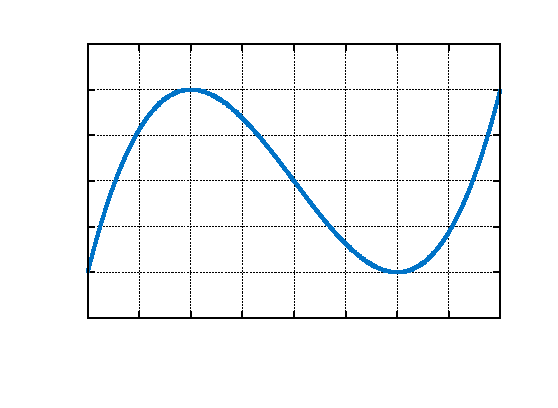
\includegraphics{calc12ex48}}%
    \gplfronttext
  \end{picture}%
\endgroup

\end{center}
\end{exmp}\vspace{-2mm}
\divider
\newpage
\begin{exmp}\label{exmp:graph2}
\noindent Sketch the graph of $f(x) ~=~ \frac{-x}{1 ~+~ x^2}$. Find all
local maxima and minima, inflection points, where the function is increasing or
decreasing, and where the function is concave up or concave down. Also indicate
any asymptotes.\vspace{1mm}
\par\noindent\emph{Solution:} Since $f'(x) = \frac{x^2 - 1}{(1+x^2)^2}$
then $x=1$ and $x=-1$ are the only critical points. And since
$f''(x) = \frac{2x\,(3 - x^2)}{(1+x^2)^3}$
then $f''(1) = \frac{1}{2} > 0$ and $f''(-1) = -\frac{1}{2} < 0$. So by the
Second Derivative Test, $f$ has a local minimum at $x=1$ and a local maximum at
$x=-1$. Since $f''(x) > 0$ for $x<-\sqrt{3}$,  $f''(x) < 0$ for $-\sqrt{3}<x<0$,
$f''(x) > 0$ for $0<x<\sqrt{3}$, and $f''(x) < 0$ for $x>\sqrt{3}$, then
$x=0,\pm\sqrt{3}$ are inflection points, $f$ is concave up for $x<-\sqrt{3}$
and for $0<x<\sqrt{3}$, and $f$ is concave down for $-\sqrt{3}<x<0$ and for
$x>\sqrt{3}$. Since $f'(x)>0$ for $x<-1$ and $x>1$ then $f$ is increasing for
$\abs{x} > 1$. And $f'(x)<0$ for $-1<x<1$ means $f$ is decreasing for
$\abs{x}<1$. Finally, since $\displaystyle\lim_{x \to \infty} f(x) = 0$ and
$\displaystyle\lim_{x \to -\infty} f(x) = 0$ then the $x$-axis ($y=0$)
is a horizontal asymptote. There are no vertical asymptotes (why?).

\par\noindent The graph is shown below:

\begin{center}
% GNUPLOT: LaTeX picture with Postscript
\begingroup
\footnotesize
  \makeatletter
  \providecommand\color[2][]{%
    \GenericError{(gnuplot) \space\space\space\@spaces}{%
      Package color not loaded in conjunction with
      terminal option `colourtext'%
    }{See the gnuplot documentation for explanation.%
    }{Either use 'blacktext' in gnuplot or load the package
      color.sty in LaTeX.}%
    \renewcommand\color[2][]{}%
  }%
  \providecommand\includegraphics[2][]{%
    \GenericError{(gnuplot) \space\space\space\@spaces}{%
      Package graphicx or graphics not loaded%
    }{See the gnuplot documentation for explanation.%
    }{The gnuplot epslatex terminal needs graphicx.sty or graphics.sty.}%
    \renewcommand\includegraphics[2][]{}%
  }%
  \providecommand\rotatebox[2]{#2}%
  \@ifundefined{ifGPcolor}{%
    \newif\ifGPcolor
    \GPcolortrue
  }{}%
  \@ifundefined{ifGPblacktext}{%
    \newif\ifGPblacktext
    \GPblacktexttrue
  }{}%
  % define a \g@addto@macro without @ in the name:
  \let\gplgaddtomacro\g@addto@macro
  % define empty templates for all commands taking text:
  \gdef\gplbacktext{}%
  \gdef\gplfronttext{}%
  \makeatother
  \ifGPblacktext
    % no textcolor at all
    \def\colorrgb#1{}%
    \def\colorgray#1{}%
  \else
    % gray or color?
    \ifGPcolor
      \def\colorrgb#1{\color[rgb]{#1}}%
      \def\colorgray#1{\color[gray]{#1}}%
      \expandafter\def\csname LTw\endcsname{\color{white}}%
      \expandafter\def\csname LTb\endcsname{\color{black}}%
      \expandafter\def\csname LTa\endcsname{\color{black}}%
      \expandafter\def\csname LT0\endcsname{\color[rgb]{1,0,0}}%
      \expandafter\def\csname LT1\endcsname{\color[rgb]{0,1,0}}%
      \expandafter\def\csname LT2\endcsname{\color[rgb]{0,0,1}}%
      \expandafter\def\csname LT3\endcsname{\color[rgb]{1,0,1}}%
      \expandafter\def\csname LT4\endcsname{\color[rgb]{0,1,1}}%
      \expandafter\def\csname LT5\endcsname{\color[rgb]{1,1,0}}%
      \expandafter\def\csname LT6\endcsname{\color[rgb]{0,0,0}}%
      \expandafter\def\csname LT7\endcsname{\color[rgb]{1,0.3,0}}%
      \expandafter\def\csname LT8\endcsname{\color[rgb]{0.5,0.5,0.5}}%
    \else
      % gray
      \def\colorrgb#1{\color{black}}%
      \def\colorgray#1{\color[gray]{#1}}%
      \expandafter\def\csname LTw\endcsname{\color{white}}%
      \expandafter\def\csname LTb\endcsname{\color{black}}%
      \expandafter\def\csname LTa\endcsname{\color{black}}%
      \expandafter\def\csname LT0\endcsname{\color{black}}%
      \expandafter\def\csname LT1\endcsname{\color{black}}%
      \expandafter\def\csname LT2\endcsname{\color{black}}%
      \expandafter\def\csname LT3\endcsname{\color{black}}%
      \expandafter\def\csname LT4\endcsname{\color{black}}%
      \expandafter\def\csname LT5\endcsname{\color{black}}%
      \expandafter\def\csname LT6\endcsname{\color{black}}%
      \expandafter\def\csname LT7\endcsname{\color{black}}%
      \expandafter\def\csname LT8\endcsname{\color{black}}%
    \fi
  \fi
    \setlength{\unitlength}{0.0500bp}%
    \ifx\gptboxheight\undefined%
      \newlength{\gptboxheight}%
      \newlength{\gptboxwidth}%
      \newsavebox{\gptboxtext}%
    \fi%
    \setlength{\fboxrule}{0.5pt}%
    \setlength{\fboxsep}{1pt}%
\begin{picture}(5040.00,3600.00)%
    \gplgaddtomacro\gplbacktext{%
      \csname LTb\endcsname%
      \put(946,704){\makebox(0,0)[r]{\strut{}$-1$}}%
      \csname LTb\endcsname%
      \put(946,1362){\makebox(0,0)[r]{\strut{}$-0.5$}}%
      \csname LTb\endcsname%
      \put(946,2020){\makebox(0,0)[r]{\strut{}$0$}}%
      \csname LTb\endcsname%
      \put(946,2677){\makebox(0,0)[r]{\strut{}$0.5$}}%
      \csname LTb\endcsname%
      \put(946,3335){\makebox(0,0)[r]{\strut{}$1$}}%
      \csname LTb\endcsname%
      \put(1078,484){\makebox(0,0){\strut{}$-4$}}%
      \csname LTb\endcsname%
      \put(1524,484){\makebox(0,0){\strut{}$-3$}}%
      \csname LTb\endcsname%
      \put(1969,484){\makebox(0,0){\strut{}$-2$}}%
      \csname LTb\endcsname%
      \put(2415,484){\makebox(0,0){\strut{}$-1$}}%
      \csname LTb\endcsname%
      \put(2861,484){\makebox(0,0){\strut{}$0$}}%
      \csname LTb\endcsname%
      \put(3306,484){\makebox(0,0){\strut{}$1$}}%
      \csname LTb\endcsname%
      \put(3752,484){\makebox(0,0){\strut{}$2$}}%
      \csname LTb\endcsname%
      \put(4197,484){\makebox(0,0){\strut{}$3$}}%
      \csname LTb\endcsname%
      \put(4643,484){\makebox(0,0){\strut{}$4$}}%
    }%
    \gplgaddtomacro\gplfronttext{%
      \csname LTb\endcsname%
      \put(176,2019){\rotatebox{-270}{\makebox(0,0){\strut{}$y$}}}%
      \put(2860,154){\makebox(0,0){\strut{}$x$}}%
    }%
    \gplbacktext
    \put(0,0){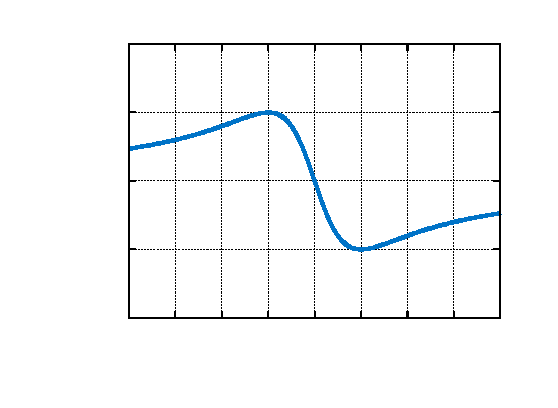
\includegraphics{calc12ex49}}%
    \gplfronttext
  \end{picture}%
\endgroup

\end{center}
\end{exmp}
\divider
\vspace{3mm}

If the Second Derivative Test fails then one alternative is the
following test:\index{First Derivative Test}

\statethm{thm:firstderivtest}{\textbf{First Derivative Test}: For a continuous
function $f$ on an interval $I$, let $x=c$ be a number in $I$ such that
$f(c)$ is defined, and either $f'(c)=0$ or $f'(c)$ does not exist. Then:
\begin{enumerate}[\bfseries (a)]
 \item If $f'(x)$ changes from negative to positive around $x=c$ then $f$ has a
  local minimum at $x=c$.
 \item If $f'(x)$ changes from positive to negative around $x=c$ then $f$ has a
  local maximum at $x=c$.
\end{enumerate}}
This test merely states the obvious: a function decreases then increases around
a minimum, and it increases then decreases around a maximum.

\begin{exmp}\label{exmp:graph3}
\parpic[r]{% GNUPLOT: LaTeX picture with Postscript
\begingroup
\footnotesize
  \makeatletter
  \providecommand\color[2][]{%
    \GenericError{(gnuplot) \space\space\space\@spaces}{%
      Package color not loaded in conjunction with
      terminal option `colourtext'%
    }{See the gnuplot documentation for explanation.%
    }{Either use 'blacktext' in gnuplot or load the package
      color.sty in LaTeX.}%
    \renewcommand\color[2][]{}%
  }%
  \providecommand\includegraphics[2][]{%
    \GenericError{(gnuplot) \space\space\space\@spaces}{%
      Package graphicx or graphics not loaded%
    }{See the gnuplot documentation for explanation.%
    }{The gnuplot epslatex terminal needs graphicx.sty or graphics.sty.}%
    \renewcommand\includegraphics[2][]{}%
  }%
  \providecommand\rotatebox[2]{#2}%
  \@ifundefined{ifGPcolor}{%
    \newif\ifGPcolor
    \GPcolortrue
  }{}%
  \@ifundefined{ifGPblacktext}{%
    \newif\ifGPblacktext
    \GPblacktexttrue
  }{}%
  % define a \g@addto@macro without @ in the name:
  \let\gplgaddtomacro\g@addto@macro
  % define empty templates for all commands taking text:
  \gdef\gplbacktext{}%
  \gdef\gplfronttext{}%
  \makeatother
  \ifGPblacktext
    % no textcolor at all
    \def\colorrgb#1{}%
    \def\colorgray#1{}%
  \else
    % gray or color?
    \ifGPcolor
      \def\colorrgb#1{\color[rgb]{#1}}%
      \def\colorgray#1{\color[gray]{#1}}%
      \expandafter\def\csname LTw\endcsname{\color{white}}%
      \expandafter\def\csname LTb\endcsname{\color{black}}%
      \expandafter\def\csname LTa\endcsname{\color{black}}%
      \expandafter\def\csname LT0\endcsname{\color[rgb]{1,0,0}}%
      \expandafter\def\csname LT1\endcsname{\color[rgb]{0,1,0}}%
      \expandafter\def\csname LT2\endcsname{\color[rgb]{0,0,1}}%
      \expandafter\def\csname LT3\endcsname{\color[rgb]{1,0,1}}%
      \expandafter\def\csname LT4\endcsname{\color[rgb]{0,1,1}}%
      \expandafter\def\csname LT5\endcsname{\color[rgb]{1,1,0}}%
      \expandafter\def\csname LT6\endcsname{\color[rgb]{0,0,0}}%
      \expandafter\def\csname LT7\endcsname{\color[rgb]{1,0.3,0}}%
      \expandafter\def\csname LT8\endcsname{\color[rgb]{0.5,0.5,0.5}}%
    \else
      % gray
      \def\colorrgb#1{\color{black}}%
      \def\colorgray#1{\color[gray]{#1}}%
      \expandafter\def\csname LTw\endcsname{\color{white}}%
      \expandafter\def\csname LTb\endcsname{\color{black}}%
      \expandafter\def\csname LTa\endcsname{\color{black}}%
      \expandafter\def\csname LT0\endcsname{\color{black}}%
      \expandafter\def\csname LT1\endcsname{\color{black}}%
      \expandafter\def\csname LT2\endcsname{\color{black}}%
      \expandafter\def\csname LT3\endcsname{\color{black}}%
      \expandafter\def\csname LT4\endcsname{\color{black}}%
      \expandafter\def\csname LT5\endcsname{\color{black}}%
      \expandafter\def\csname LT6\endcsname{\color{black}}%
      \expandafter\def\csname LT7\endcsname{\color{black}}%
      \expandafter\def\csname LT8\endcsname{\color{black}}%
    \fi
  \fi
    \setlength{\unitlength}{0.0500bp}%
    \ifx\gptboxheight\undefined%
      \newlength{\gptboxheight}%
      \newlength{\gptboxwidth}%
      \newsavebox{\gptboxtext}%
    \fi%
    \setlength{\fboxrule}{0.5pt}%
    \setlength{\fboxsep}{1pt}%
\begin{picture}(3600.00,2160.00)%
    \gplgaddtomacro\gplbacktext{%
      \csname LTb\endcsname%
      \put(814,704){\makebox(0,0)[r]{\strut{}$0$}}%
      \csname LTb\endcsname%
      \put(814,874){\makebox(0,0)[r]{\strut{}$0.2$}}%
      \csname LTb\endcsname%
      \put(814,1044){\makebox(0,0)[r]{\strut{}$0.4$}}%
      \csname LTb\endcsname%
      \put(814,1214){\makebox(0,0)[r]{\strut{}$0.6$}}%
      \csname LTb\endcsname%
      \put(814,1385){\makebox(0,0)[r]{\strut{}$0.8$}}%
      \csname LTb\endcsname%
      \put(814,1555){\makebox(0,0)[r]{\strut{}$1$}}%
      \csname LTb\endcsname%
      \put(814,1725){\makebox(0,0)[r]{\strut{}$1.2$}}%
      \csname LTb\endcsname%
      \put(814,1895){\makebox(0,0)[r]{\strut{}$1.4$}}%
      \csname LTb\endcsname%
      \put(946,484){\makebox(0,0){\strut{}$-2$}}%
      \csname LTb\endcsname%
      \put(1228,484){\makebox(0,0){\strut{}$-1.5$}}%
      \csname LTb\endcsname%
      \put(1510,484){\makebox(0,0){\strut{}$-1$}}%
      \csname LTb\endcsname%
      \put(1792,484){\makebox(0,0){\strut{}$-0.5$}}%
      \csname LTb\endcsname%
      \put(2075,484){\makebox(0,0){\strut{}$0$}}%
      \csname LTb\endcsname%
      \put(2357,484){\makebox(0,0){\strut{}$0.5$}}%
      \csname LTb\endcsname%
      \put(2639,484){\makebox(0,0){\strut{}$1$}}%
      \csname LTb\endcsname%
      \put(2921,484){\makebox(0,0){\strut{}$1.5$}}%
      \csname LTb\endcsname%
      \put(3203,484){\makebox(0,0){\strut{}$2$}}%
    }%
    \gplgaddtomacro\gplfronttext{%
      \csname LTb\endcsname%
      \put(176,1299){\rotatebox{-270}{\makebox(0,0){\strut{}$y$}}}%
      \put(2074,154){\makebox(0,0){\strut{}$x$}}%
    }%
    \gplbacktext
    \put(0,0){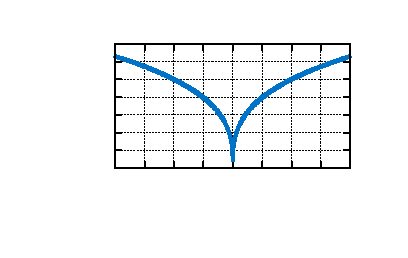
\includegraphics{calc12ex410}}%
    \gplfronttext
  \end{picture}%
\endgroup
}
\noindent Sketch the graph of $f(x) = x^{2/3}$.\vspace{1mm}
\par\noindent\emph{Solution:} Clearly $f(x)$ is continuous for all $x$,
including $x=0$ (since $f(0)=0$), but $f'(x) = \frac{2}{3\,\sqrt[3]{x}}$ is not
defined at $x=0$. Since $f'(x)$ changes from negative to positive around $x=0$
($f'(x) < 0$ when $x < 0$ and $f'(x) > 0$ when $x > 0$), then by the First
Derivative Test $f$ has a local minimum at $x=0$. Since $f''(x) = -\,
\frac{2}{9\,x^{4/3}} < 0$ for all $x \ne 0$, then $f$ is always concave down.
There are no vertical or horizontal asymptotes. The graph is shown on the
right.\vspace{2mm}
\picskip{0}
\par\noindent Note that the Second Derivative Test could not be used for this
function, since $f'(x) \ne 0$ for all $x$ (notice also that $f''(x)$ is not
defined at $x=0$).
\end{exmp}
\divider
\vspace{3mm}

A more complete alternative to the Second Derivative Test is the
following:\footnote{For a proof, see pp.10-11 in
\textsc{Koo, D.}, \emph{Elements of Optimization}, New York: Springer-Verlag,
1977.}\index{Nth Derivative Test@N\textsuperscript{th} Derivative Test}

\statethm{thm:nderivtest}{\textbf{N\textsuperscript{th} Derivative Test}: A
non-constant
function $f$ with continuous derivatives of all orders up to and including
$n >1$ at $x=c$ has either a local minimum, local maximum or inflection point at
$x=c$ if and only if
\[
f^{(k)}(c) ~=~ 0 ~~\text{for $k=1$, $2$, $\ldots$, $n-1$}
\quad\text{and}\quad f^{(n)}(c) ~\ne~ 0
\]
(i.e. the $n^{\text{th}}$ derivative is the first nonzero derivative at $x=c$).
If so, then:

\begin{enumerate}[\bfseries (a)]
 \item If $n>1$ is even and $f^{(n)}(c) > 0$ then $f$ has a
  local minimum at $x=c$.
 \item If $n>1$ is even and $f^{(n)}(c) < 0$ then $f$ has a
  local maximum at $x=c$.
 \item If $n>1$ is odd then $f$ has an inflection point at $x=c$.
\end{enumerate}}
Note that the Second Derivative Test is the special case where $n=2$ in the
N\textsuperscript{th} Derivative Test. Though this test gives necessary
and sufficient conditions for a local maximum, local minimum, and inflection
point, calculating the first $n$ derivatives can be complicated if $n$ is large
and the given function is not simple.

\begin{exmp}\label{exmp:graph4}
The Second Derivative Test fails for $f(x)=x^4$ at the critical point $x=0$,
since $f''(0)=0$. But the first 4 derivatives of $f(x)=x^4$ are $f'(x)=4x^3$,
$f''(x)=12x^2$, $f^{(3)}(x)=24x$, and $f^{(4)}(x)=24$, which are all continuous
and
\[
f^{(k)}(0) ~=~ 0 ~~\text{for $k=1$, $2$, $3$}
\quad\text{and}\quad f^{(4)}(0) ~=~ 24 ~\ne~ 0 ~.
\]
So by the
N\textsuperscript{th} Derivative Test, since $n=4$ is even and $f^{(4)}(0)=24>0$
then $f(x)=x^4$ has a local minimum at $x=0$. Note that $f(x) \ge 0 = f(0)$ for
all $x$, so $x = 0$ is actually a global minimum for $f$.
\end{exmp}
\divider
\newpage
A common practice in many fields of science and engineering is to combine
multiple named constants (e.g. $\pi$) or variables in a function into one
variable and then sketch a graph of that function. The example below illustrates
the technique.

\begin{exmp}\label{exmp:graph5}
\noindent A hydrogen atom has one electron, and the probability of finding the
electron in the ground state of the hydrogen atom between radii $r$ and $r+\dr$
is $D(r)\,\dr$, where $\dr$ is an infinitesimal change in the radius $r$ (the
distance from the electron to the nucleus), $D(r)$ is the \emph{radial
probability density function}
\[
D(r) ~=~ \frac{4}{a_0^3}\,r^2 e^{-2r/a_0}
\]
and $a_0 \approx 5.291772 \times 10^{-11}$ m is the \emph{Bohr radius}\index{Bohr
radius}. It is useful to analyze this function in terms of $r \ge 0$
in relation to the Bohr radius $a_0$ (e.g.
$r= 0.5a_0$, $a_0$, $2a_0$, $3a_0$). To do this, let $x = \frac{r}{a_0}$, so that
\[
D(r) ~=~ \frac{4}{a_0}\,\left(\frac{r}{a_0}\right)^2 e^{-2\left(\frac{r}{a_0}\right)}
\quad\Rightarrow\quad
a_0\,D(x) ~=~ 4x^2 e^{-2x}
\]
and then sketch the graph of $a_0\,D(x)$, which is shown below:

\begin{center}
% GNUPLOT: LaTeX picture with Postscript
\begingroup
\footnotesize
  \makeatletter
  \providecommand\color[2][]{%
    \GenericError{(gnuplot) \space\space\space\@spaces}{%
      Package color not loaded in conjunction with
      terminal option `colourtext'%
    }{See the gnuplot documentation for explanation.%
    }{Either use 'blacktext' in gnuplot or load the package
      color.sty in LaTeX.}%
    \renewcommand\color[2][]{}%
  }%
  \providecommand\includegraphics[2][]{%
    \GenericError{(gnuplot) \space\space\space\@spaces}{%
      Package graphicx or graphics not loaded%
    }{See the gnuplot documentation for explanation.%
    }{The gnuplot epslatex terminal needs graphicx.sty or graphics.sty.}%
    \renewcommand\includegraphics[2][]{}%
  }%
  \providecommand\rotatebox[2]{#2}%
  \@ifundefined{ifGPcolor}{%
    \newif\ifGPcolor
    \GPcolortrue
  }{}%
  \@ifundefined{ifGPblacktext}{%
    \newif\ifGPblacktext
    \GPblacktexttrue
  }{}%
  % define a \g@addto@macro without @ in the name:
  \let\gplgaddtomacro\g@addto@macro
  % define empty templates for all commands taking text:
  \gdef\gplbacktext{}%
  \gdef\gplfronttext{}%
  \makeatother
  \ifGPblacktext
    % no textcolor at all
    \def\colorrgb#1{}%
    \def\colorgray#1{}%
  \else
    % gray or color?
    \ifGPcolor
      \def\colorrgb#1{\color[rgb]{#1}}%
      \def\colorgray#1{\color[gray]{#1}}%
      \expandafter\def\csname LTw\endcsname{\color{white}}%
      \expandafter\def\csname LTb\endcsname{\color{black}}%
      \expandafter\def\csname LTa\endcsname{\color{black}}%
      \expandafter\def\csname LT0\endcsname{\color[rgb]{1,0,0}}%
      \expandafter\def\csname LT1\endcsname{\color[rgb]{0,1,0}}%
      \expandafter\def\csname LT2\endcsname{\color[rgb]{0,0,1}}%
      \expandafter\def\csname LT3\endcsname{\color[rgb]{1,0,1}}%
      \expandafter\def\csname LT4\endcsname{\color[rgb]{0,1,1}}%
      \expandafter\def\csname LT5\endcsname{\color[rgb]{1,1,0}}%
      \expandafter\def\csname LT6\endcsname{\color[rgb]{0,0,0}}%
      \expandafter\def\csname LT7\endcsname{\color[rgb]{1,0.3,0}}%
      \expandafter\def\csname LT8\endcsname{\color[rgb]{0.5,0.5,0.5}}%
    \else
      % gray
      \def\colorrgb#1{\color{black}}%
      \def\colorgray#1{\color[gray]{#1}}%
      \expandafter\def\csname LTw\endcsname{\color{white}}%
      \expandafter\def\csname LTb\endcsname{\color{black}}%
      \expandafter\def\csname LTa\endcsname{\color{black}}%
      \expandafter\def\csname LT0\endcsname{\color{black}}%
      \expandafter\def\csname LT1\endcsname{\color{black}}%
      \expandafter\def\csname LT2\endcsname{\color{black}}%
      \expandafter\def\csname LT3\endcsname{\color{black}}%
      \expandafter\def\csname LT4\endcsname{\color{black}}%
      \expandafter\def\csname LT5\endcsname{\color{black}}%
      \expandafter\def\csname LT6\endcsname{\color{black}}%
      \expandafter\def\csname LT7\endcsname{\color{black}}%
      \expandafter\def\csname LT8\endcsname{\color{black}}%
    \fi
  \fi
    \setlength{\unitlength}{0.0500bp}%
    \ifx\gptboxheight\undefined%
      \newlength{\gptboxheight}%
      \newlength{\gptboxwidth}%
      \newsavebox{\gptboxtext}%
    \fi%
    \setlength{\fboxrule}{0.5pt}%
    \setlength{\fboxsep}{1pt}%
\begin{picture}(5040.00,3600.00)%
    \gplgaddtomacro\gplbacktext{%
      \csname LTb\endcsname%
      \put(814,704){\makebox(0,0)[r]{\strut{}$0$}}%
      \csname LTb\endcsname%
      \put(814,1143){\makebox(0,0)[r]{\strut{}$0.1$}}%
      \csname LTb\endcsname%
      \put(814,1581){\makebox(0,0)[r]{\strut{}$0.2$}}%
      \csname LTb\endcsname%
      \put(814,2020){\makebox(0,0)[r]{\strut{}$0.3$}}%
      \csname LTb\endcsname%
      \put(814,2458){\makebox(0,0)[r]{\strut{}$0.4$}}%
      \csname LTb\endcsname%
      \put(814,2896){\makebox(0,0)[r]{\strut{}$0.5$}}%
      \csname LTb\endcsname%
      \put(814,3335){\makebox(0,0)[r]{\strut{}$0.6$}}%
      \csname LTb\endcsname%
      \put(946,484){\makebox(0,0){\strut{}$0$}}%
      \csname LTb\endcsname%
      \put(1562,484){\makebox(0,0){\strut{}$1$}}%
      \csname LTb\endcsname%
      \put(2178,484){\makebox(0,0){\strut{}$2$}}%
      \csname LTb\endcsname%
      \put(2795,484){\makebox(0,0){\strut{}$3$}}%
      \csname LTb\endcsname%
      \put(3411,484){\makebox(0,0){\strut{}$4$}}%
      \csname LTb\endcsname%
      \put(4027,484){\makebox(0,0){\strut{}$5$}}%
      \csname LTb\endcsname%
      \put(4643,484){\makebox(0,0){\strut{}$6$}}%
    }%
    \gplgaddtomacro\gplfronttext{%
      \csname LTb\endcsname%
      \put(176,2019){\rotatebox{-270}{\makebox(0,0){\strut{}$a_0 D\left(\tfrac{r}{a_0}\right)$}}}%
      \put(2794,154){\makebox(0,0){\strut{}$\frac{r}{a_0}$}}%
    }%
    \gplbacktext
    \put(0,0){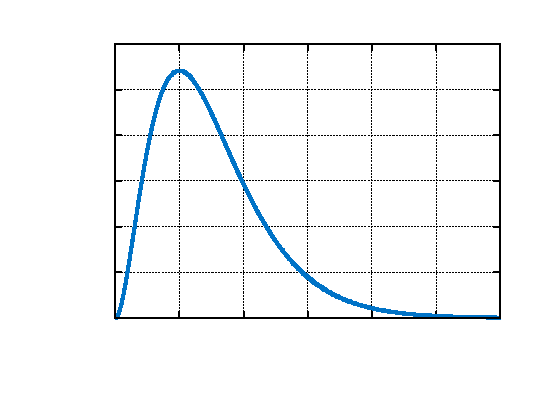
\includegraphics{calc12ex412}}%
    \gplfronttext
  \end{picture}%
\endgroup

\end{center}

\noindent From the graph it looks like $x=1$ (i.e. $r = a_0$) is a local (and
global) maximum, so that the electron is most likely to be found near
$r = a_0$, and the probability drops off dramatically past a distance
$r = 3a_0$. In the exercises you will be asked to show that $r = a_0$ is indeed
a local maximum and that the inflection points are
$r = \left(1 \pm \frac{1}{\sqrt{2}}\right)\,a_0$.\vspace{2mm}

\par\noindent Note that the right side of the formula
$a_0\,D(x) = 4x^2 e^{-2x}$ does not involve $a_0$, which was multiplied
over to the left side. In general that is the strategy when dealing with
these sorts of functions where variables and constants are combined. In this
case the stray constant $a_0$ can be multiplied with $D$ since that will not
affect the location of critical and inflection points, nor fundamentally alter
the general shape of the graph.
\end{exmp}
\divider
\newpage
\begin{exmp}\label{exmp:thermalex}
\noindent For a single particle with two states---energy 0 and energy
$\epsilon$---in thermal contact with a reservoir at temperature $\tau$, the
average energy $U$ and heat capacity $C_V$ are given by
\[
U ~=~ \epsilon\,\frac{e^{-\epsilon/\tau}}{1 + e^{-\epsilon/\tau}} \quad\text{and}\quad
C_V ~=~ k_B\,\left(\frac{\epsilon}{\tau}\right)^2 \frac{e^{\epsilon/\tau}}{\left(1 + e^{\epsilon/\tau}\right)^2}
\]
where $k_B \approx 1.38065 \times 10^{\text{$-$}23}$ J/K is the
\emph{Boltzmann constant}. The graph below shows both quantities as functions
of $\tau/\epsilon$ (\emph{not} $\epsilon/\tau$, as you might
expect). See Exercise \ref{exer:thermalex}.\vspace{-3mm}

\begin{center}
% GNUPLOT: LaTeX picture with Postscript
\begingroup
  \makeatletter
  \providecommand\color[2][]{%
    \GenericError{(gnuplot) \space\space\space\@spaces}{%
      Package color not loaded in conjunction with
      terminal option `colourtext'%
    }{See the gnuplot documentation for explanation.%
    }{Either use 'blacktext' in gnuplot or load the package
      color.sty in LaTeX.}%
    \renewcommand\color[2][]{}%
  }%
  \providecommand\includegraphics[2][]{%
    \GenericError{(gnuplot) \space\space\space\@spaces}{%
      Package graphicx or graphics not loaded%
    }{See the gnuplot documentation for explanation.%
    }{The gnuplot epslatex terminal needs graphicx.sty or graphics.sty.}%
    \renewcommand\includegraphics[2][]{}%
  }%
  \providecommand\rotatebox[2]{#2}%
  \@ifundefined{ifGPcolor}{%
    \newif\ifGPcolor
    \GPcolortrue
  }{}%
  \@ifundefined{ifGPblacktext}{%
    \newif\ifGPblacktext
    \GPblacktexttrue
  }{}%
  % define a \g@addto@macro without @ in the name:
  \let\gplgaddtomacro\g@addto@macro
  % define empty templates for all commands taking text:
  \gdef\gplbacktext{}%
  \gdef\gplfronttext{}%
  \makeatother
  \ifGPblacktext
    % no textcolor at all
    \def\colorrgb#1{}%
    \def\colorgray#1{}%
  \else
    % gray or color?
    \ifGPcolor
      \def\colorrgb#1{\color[rgb]{#1}}%
      \def\colorgray#1{\color[gray]{#1}}%
      \expandafter\def\csname LTw\endcsname{\color{white}}%
      \expandafter\def\csname LTb\endcsname{\color{black}}%
      \expandafter\def\csname LTa\endcsname{\color{black}}%
      \expandafter\def\csname LT0\endcsname{\color[rgb]{1,0,0}}%
      \expandafter\def\csname LT1\endcsname{\color[rgb]{0,1,0}}%
      \expandafter\def\csname LT2\endcsname{\color[rgb]{0,0,1}}%
      \expandafter\def\csname LT3\endcsname{\color[rgb]{1,0,1}}%
      \expandafter\def\csname LT4\endcsname{\color[rgb]{0,1,1}}%
      \expandafter\def\csname LT5\endcsname{\color[rgb]{1,1,0}}%
      \expandafter\def\csname LT6\endcsname{\color[rgb]{0,0,0}}%
      \expandafter\def\csname LT7\endcsname{\color[rgb]{1,0.3,0}}%
      \expandafter\def\csname LT8\endcsname{\color[rgb]{0.5,0.5,0.5}}%
    \else
      % gray
      \def\colorrgb#1{\color{black}}%
      \def\colorgray#1{\color[gray]{#1}}%
      \expandafter\def\csname LTw\endcsname{\color{white}}%
      \expandafter\def\csname LTb\endcsname{\color{black}}%
      \expandafter\def\csname LTa\endcsname{\color{black}}%
      \expandafter\def\csname LT0\endcsname{\color{black}}%
      \expandafter\def\csname LT1\endcsname{\color{black}}%
      \expandafter\def\csname LT2\endcsname{\color{black}}%
      \expandafter\def\csname LT3\endcsname{\color{black}}%
      \expandafter\def\csname LT4\endcsname{\color{black}}%
      \expandafter\def\csname LT5\endcsname{\color{black}}%
      \expandafter\def\csname LT6\endcsname{\color{black}}%
      \expandafter\def\csname LT7\endcsname{\color{black}}%
      \expandafter\def\csname LT8\endcsname{\color{black}}%
    \fi
  \fi
    \setlength{\unitlength}{0.0500bp}%
    \ifx\gptboxheight\undefined%
      \newlength{\gptboxheight}%
      \newlength{\gptboxwidth}%
      \newsavebox{\gptboxtext}%
    \fi%
    \setlength{\fboxrule}{0.5pt}%
    \setlength{\fboxsep}{1pt}%
\begin{picture}(7200.00,4032.00)%
    \gplgaddtomacro\gplbacktext{%
      \csname LTb\endcsname%
      \put(726,704){\makebox(0,0)[r]{\strut{}$0$}}%
      \put(726,971){\makebox(0,0)[r]{\strut{}$0.05$}}%
      \put(726,1237){\makebox(0,0)[r]{\strut{}$0.1$}}%
      \put(726,1504){\makebox(0,0)[r]{\strut{}$0.15$}}%
      \put(726,1771){\makebox(0,0)[r]{\strut{}$0.2$}}%
      \put(726,2038){\makebox(0,0)[r]{\strut{}$0.25$}}%
      \put(726,2304){\makebox(0,0)[r]{\strut{}$0.3$}}%
      \put(726,2571){\makebox(0,0)[r]{\strut{}$0.35$}}%
      \put(726,2838){\makebox(0,0)[r]{\strut{}$0.4$}}%
      \put(726,3104){\makebox(0,0)[r]{\strut{}$0.45$}}%
      \put(726,3371){\makebox(0,0)[r]{\strut{}$0.5$}}%
      \put(858,484){\makebox(0,0){\strut{}$0$}}%
      \put(2047,484){\makebox(0,0){\strut{}$1$}}%
      \put(3236,484){\makebox(0,0){\strut{}$2$}}%
      \put(4425,484){\makebox(0,0){\strut{}$3$}}%
      \put(5614,484){\makebox(0,0){\strut{}$4$}}%
      \put(6803,484){\makebox(0,0){\strut{}$5$}}%
    }%
    \gplgaddtomacro\gplfronttext{%
      \csname LTb\endcsname%
      \put(3830,154){\makebox(0,0){\strut{}$\tau/\epsilon$}}%
      \put(3830,3701){\makebox(0,0){\strut{}Average Energy $U/\epsilon$ vs Heat Capacity $C_V/k_B$}}%
      \csname LTb\endcsname%
      \put(5816,2509){\makebox(0,0)[r]{\strut{}$U/\epsilon = \dfrac{e^{-\epsilon/\tau}}{1 + e^{-\epsilon/\tau}}$}}%
      \csname LTb\endcsname%
      \put(5816,1564){\makebox(0,0)[r]{\strut{}$C_V/k_B = \left(\dfrac{\epsilon}{\tau}\right)^2 \dfrac{e^{\epsilon/\tau}}{\left(1 + e^{\epsilon/\tau}\right)^2}$}}%
    }%
    \gplbacktext
    \put(0,0){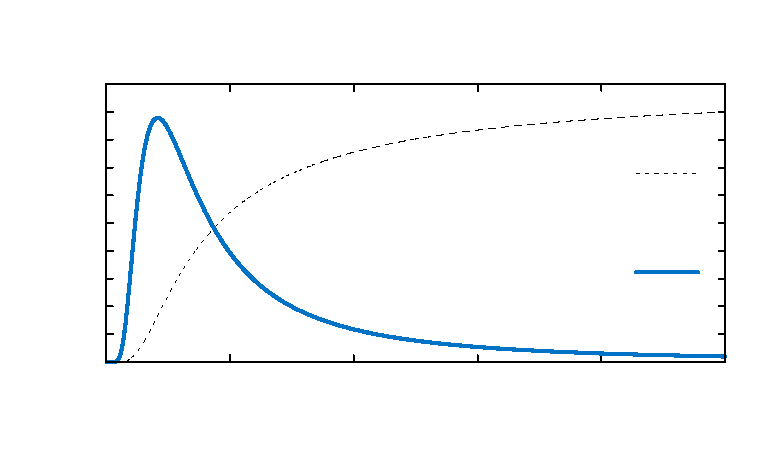
\includegraphics{thermalex}}%
    \gplfronttext
  \end{picture}%
\endgroup

\end{center}
\end{exmp}\vspace{-4mm}
\divider
\vspace{3mm}
\startexercises\label{sec4dot2}
{\small
\probs{A}
\par\noindent For Exercises 1-8 sketch the graph of the given function. Find all
local maxima and minima, inflection points, where the function is increasing or
decreasing, where the function is concave up or concave down, and indicate any
asymptotes.
\begin{enumerate}[\bfseries 1.]
 \begin{multicols}{4}
  \item $f(x) ~=~ x^3 - 3x\vphantom{;e^{-x^2}}$
  \item $f(x) ~=~ x^3 - 3x^2 + 1\vphantom{;e^{-x^2}}$
  \item $f(x) ~=~ xe^{-x}\vphantom{;e^{-x^2}}$
  \item $f(x) ~=~ x^2 \;e^{-x^2}$
 \end{multicols}
 \begin{multicols}{4}
  \item $f(x) ~=~ \dfrac{1}{1 ~+~ x^2}\vphantom{\dfrac{e^{-x} ~-~ e^{-2x}}{2}}$
  \item $f(x) ~=~ \dfrac{x^2}{(x - 1)^2}\vphantom{\dfrac{e^{-x} ~-~ e^{-2x}}{2}}$
  \item $f(x) ~=~ \dfrac{e^{-x} ~-~ e^{-2x}}{2}$
  \item $f(x) ~=~ e^{-x}\;\sin\,x\vphantom{\dfrac{e^{-x} ~-~ e^{-2x}}{2}}$
 \end{multicols}
  \item\label{exer:thermalex} Write $U/\epsilon$ and $C_V/k_B$ from Example
   \ref{exmp:thermalex} as functions of $x=\tau/\epsilon$. You do not need to
   sketch the graphs.
 \item Show that the function $D(r) = \frac{4}{a_0^3}\,r^2 e^{-2r/a_0}$ from Example
  \ref{exmp:graph5} has a local maximum at $r=a_0$ and inflection points at
  $r = \left(1 \pm \frac{1}{\sqrt{2}}\right)\,a_0$.
 \item Sketch the graph of \emph{Kratzer's molecular potential}
  $V(r) = -2D\,\left(\frac{a}{r} - \frac{1}{2} \frac{a^2}{r^2}\right)$ as a
  function of $x=\frac{r}{a}$, with $a > 0$ and $D > 0$ as constants.
 \item Sketch the graph of
  $f(K) = \frac{2N\sqrt{K}\,e^{-\frac{K}{kT}}}{\sqrt{\pi}\,(kT)^{3/2}}$ as a
  function of $x=\frac{K}{kT}$, with $N$, $k$ and $T$ as positive constants.
 \item Prove part (b) of the Concavity Theorem.
\end{enumerate}
}
\newpage
%Begin Section 4.3
\section{Numerical Approximation of Roots of Functions}
When finding critical points of a function $f$, you encounter the problem of
solving the equation $f'(x)=0$. The examples and exercises so far were set up
carefully so that solutions to that equation could be found in a simple closed
form. But in practice this will not always be the case---in fact it is
\emph{almost never} the case.\index{root of function}\index{function!root}
For example, finding the critical points of the function
$f(x) = \sin\,x \;-\; \frac{x^2}{2}$
entails solving the equation $f'(x) = \cos\,x \;-\; x ~=~ 0$, for which there is
no solution in a closed-form expression.

What should you do in such a situation?\footnote{Note: To ``just give up''---as
suggested semi-seriously by some students I have had---is not an option.}  One
possibility is to use the bisection method\index{bisection method} mentioned in
Section 3.3. In fact, in Example \ref{exmp:ivt} the solution to the equation
$\cos\,x = x$ (i.e. $\cos\,x \;-\; x \;=\;0$) was shown to exist in the interval
$\ival{0}{1}$, and then a demonstration of the bisection method was given to
find that solution.

The bisection method is one of many \emph{numerical methods} for finding roots
of a function (i.e. where the function is zero). Finding the critical points of
a function means finding the roots of its derivative. Though the bisection
method could be used for that purpose, convergence to each root is usually
slow.\index{Newton's method} A far more efficient method is
\textbf{Newton's method}\footnote{Sometimes called the \emph{Newton-Raphson
method}.}, whose geometric interpretation is shown in Figure \ref{fig:newton}
below.

\begin{figure}[ht]
 \centering
 \begin{tikzpicture}[>=latex,every node/.style={font=\small}]
  \draw [black!60,line width=1pt,->] (0,-1) -- (0,4.5) node[above] {$y$};
  \draw [name path=xaxis,black!60,line width=1pt,->] (-1.5,0) -- (9.5,0) node[right] {$x$};
  \draw[name path=x0vert,white] (7.5,0.4) -- (7.5,4.5);
  \draw[name path=x1vert,white] (5,0.2) -- (5,2);
  \draw[name path=curve,linecolor,line width=1.5pt] (0.5,-1) parabola (8,4.5);
  \fill [name intersections={of=curve and xaxis,by={x}}] (x) circle (2.5pt);
  \fill [name intersections={of=curve and x0vert,by={f0}}] (f0) circle (2.5pt);
  \fill [name intersections={of=curve and x1vert,by={f1}}] (f1) circle (2.5pt);
  \node[below left] at (0,0) {$0$};
  \node[above] at (6,3) {$y=f(x)$};
  \node[below] at (x) {$\bar{x}$};
  \node[below] at (7.5,0) {$x_0$};
  \draw[dashed] (7.5,0.02) -- (f0);
  \node[right] at (f0) {$(x_0,f(x_0))$};
  \draw[red,line width=0.6pt] (f0) -- (5,0.02);
  \node[below] at (5,0) {$x_1$};
  \draw[dashed] (5,0.02) -- (f1);
  \node[left] at (f1) {$(x_1,f(x_1))$};
  \draw[red,line width=0.6pt] (f1) -- (4.05,0.02);
  \node[below] at (4.05,0) {$x_2$};
 \end{tikzpicture}
 \caption[]{\quad Newton's method for finding a root $\bar{x}$ of $f(x)$}
 \label{fig:newton}
\end{figure}

\noindent The idea behind Newton's method is simple: to find a root $\bar{x}$ of
a function $f$, choose an \emph{initial guess} $x_0$ and then go up---or
down---to the curve $y=f(x)$ and draw the tangent line to the curve at the
point $(x_0,f(x_0))$. Let $x_1$ be where that tangent line intersects the
$x$-axis, as shown above; repeat this procedure on $x_1$ to get the next number
$x_2$, repeat on $x_2$ to get $x_3$, and so on. The resulting sequence of
numbers $x_0$, $x_1$, $x_2$, $x_3$, $\ldots$, will approach the root $\bar{x}$.
Convergence under certain conditions can be proved.\footnote{See pp.58-62 in
\textsc{Saaty, T.L. and J. Bram}, \emph{Nonlinear Mathematics}, New York:
McGraw-Hill, Inc., 1964.}
\newpage
The general formula for the number $x_n$ obtained after $n \ge 1$ iterations in
Newton's method can be determined by considering the formula for $x_1$. First,
the tangent line to $y=f(x)$ at the point $(x_0,f(x_0))$ has slope $f'(x_0)$, so
the equation of the line is
\begin{equation}\label{eqn:newton}
y ~-~ f(x_0) ~=~ f'(x_0)\,(x ~-~ x_0) ~.
\end{equation}
 The point $(x_1,0)$ is (by design) also on that line, so that
\[
0 ~-~ f(x_0) ~=~ f'(x_0)\,(x_1 ~-~ x_0) \quad\Rightarrow\quad
x_1 ~=~ x_0 ~-~ \frac{f(x_0)}{f'(x_0)}
\]
provided that $f'(x_0) \ne 0$. The general formula for $x_n$ is given by the
following algorithm:

\statedefn{defn:newton}{\textbf{Newton's method}: For an initial guess $x_0$,
the numbers $x_n$ for $n \ge 1$ are computed iteratively as:
\[
x_n ~=~ x_{n-1} ~-~ \frac{f(x_{n-1})}{f'(x_{n-1})} \qquad\text{for $n =1$, $2$,
$3$, $\ldots$}
\]
That is, each ``next'' number $x_n$ depends on the previous number $x_{n-1}$.
The algorithm terminates whenever $f'(x_n)=0$, or when the desired accuracy is
reached. If $f'(x_n)=0$ for some $n \ge 0$, then you could start over with a
different initial guess $x_0$.}

To implement this algorithm in a programming language (for which Newton's
method is well-suited), the following language-independent \emph{pseudocode}
can be used as a guide:

\statecor{cor:newtonalg}{\begin{center}
 \textbf{Algorithm pseudocode for Newton's method}
\end{center}
\begin{codebox}
\Procname{$\proc{Newton's method}$}
\li $N \gets \const{Number-of-iterations}$\>\>\>\>\>\>\>\>\>\Comment User supplies this value
\li $x \gets \const{initial-guess}$\>\>\>\>\>\>\>\>\>\Comment User supplies this value
\li \For $n \gets 1$ \To $N$
\li    \Do
\li       \If $f'(x) \neq 0$
\li          \Then
\li             $x \gets x ~-~ \dfrac{f(x)}{f'(x)}$
\li             print $x$
\li       \Else
\li          \Error ``division by zero''
          \End
       \End
\end{codebox}}
\newpage
\begin{exmp}\label{exmp:newt1}
\noindent Use Newton's method to find the root of $f(x) = \cos\,x - x$.\vspace{1mm}
\par\noindent\emph{Solution:} Since the root is already known to be in the
interval $\ival{0}{1}$, choose $x_0 = 1$ as the initial guess. The numbers
$x_n$ for $n \ge 1$ can be computed with a hand-held scientific calculator, but
the process is tedious and error-prone. Using a computer is far more efficient
and allows more flexibility.

For example, the algorithm is easily implemented in the Java programming
language. Save this code in a plain text file as \texttt{newton.java}:
\lstset{language=Java,showstringspaces=false,lineskip=0.3pt,xleftmargin=0.06\textwidth,
basicstyle={\small\fontfamily{fvm}\fontseries{m}\selectfont},
keywordstyle={\small\fontfamily{fvm}\fontseries{b}\selectfont},
numberstyle={\color{linenumcolor}\footnotesize\fontfamily{fvm}\fontseries{m}\selectfont},
breaklines=true,columns=fullflexible,backgroundcolor=\color{codecolor},numbers=left,
linewidth=0.95\textwidth,keepspaces=true,float=h,
caption={\quad Newton's method in Java (\texttt{newton.java})},numbersep=15pt,
label=newt1java}
\begin{lstlisting}[frame=single,framerule=0pt]
public class newton {
   public static void main(String[] args) {
      int N = Integer.parseInt(args[0]); //Number of iterations
      double x = 1.0; //initial guess
      System.out.println("n=0: " + x);
      for (int i = 1; i <= N; i++) {
         x =  x - f(x)/derivf(x);
         System.out.println("n=" + i + ": " + x);
      }
   }
 
   //Define the function f(x)
   public static double f(double x) {
      return Math.cos(x) - x;
   }

   //Define the derivative f'(x)
   public static double derivf(double x) {
      return -Math.sin(x) - 1.0;
   }
}
\end{lstlisting}
\noindent Though knowledge of Java would help, it should not be that difficult
to figure out what the above code is doing. The number of iterations $N$ is
passed as a command-line parameter to the program, and $x_n$ is computed and
printed for $n=0$, $1$, $2$, $\ldots$ , $N$. Note that the derivative of $f(x)$
is ``hard-coded'' into the program.\footnote{There are some programming
language libraries for
calculating derivatives of functions ``on the fly,'' i.e. dynamically. For
example, the \textbf{GNU libmatheval} C/Fortran library can perform such
symbolic operations. It is available at
\url{http://www.gnu.org/software/libmatheval/}}
There is also no error checking for the derivative being zero at any $x_n$.
The program would simply halt on a division by zero error.

Compile the code, then run the program with $10$ iterations:
\begin{Verbatim}[frame=single,framesep=3pt]
javac newton.java
java newton 10
\end{Verbatim}
The output is shown below:

\begin{Verbatim}[frame=single,framesep=3pt]
n=0: 1.0
n=1: 0.7503638678402439
n=2: 0.7391128909113617
n=3: 0.739085133385284
n=4: 0.7390851332151607
n=5: 0.7390851332151607
n=6: 0.7390851332151607
n=7: 0.7390851332151607
n=8: 0.7390851332151607
n=9: 0.7390851332151607
n=10: 0.7390851332151607
\end{Verbatim}
Note that the solution $\bar{x} = 0.7390851332151607$ was found after only 4
iterations; the numbers $x_n$ repeat for $n \ge 5$. This is much faster than the
bisection method.
\end{exmp}
\divider
\vspace{3mm}

Another root-finding numerical method similar to Newton's method is the
\textbf{secant method}, whose geometric interpretation is shown in Figure
\ref{fig:secant} below:\index{secant method}

\begin{figure}[ht]
 \centering
 \begin{tikzpicture}[>=latex,every node/.style={font=\small}]
  \draw [black!60,line width=1pt,->] (0,-1) -- (0,4.5) node[above] {$y$};
  \draw [name path=xaxis,black!60,line width=1pt,->] (-1.5,0) -- (9.5,0) node[right] {$x$};
  \draw[name path=x0vert,white] (7.5,0.4) -- (7.5,4.5);
  \draw[name path=x1vert,white] (5,0.2) -- (5,2);
  \draw[name path=curve,linecolor,line width=1.5pt] (0.5,-1) parabola (8,4.5);
  \fill [name intersections={of=curve and xaxis,by={x}}] (x) circle (2.5pt);
  \fill [name intersections={of=curve and x0vert,by={f0}}] (f0) circle (2.5pt);
  \fill [name intersections={of=curve and x1vert,by={f1}}] (f1) circle (2.5pt);
  \node[below left] at (0,0) {$0$};
  \node[above] at (6,3) {$y=f(x)$};
  \node[below] at (x) {$\bar{x}$};
  \node[below] at (7.5,0) {$x_0$};
  \draw[dashed] (7.5,0.02) -- (f0);
  \node[right] at (f0) {$(x_0,f(x_0))$};
  \draw[red,line width=0.6pt] (f0) -- (f1);
  \node[below] at (5,0) {$x_1$};
  \draw[dashed] (5,0.02) -- (f1);
  \node[left] at (f1) {$(x_1,f(x_1))$};
  \draw[red,line width=0.6pt] (f1) -- (4.05,0.02);
  \node[below] at (4.05,0) {$x_2$};
 \end{tikzpicture}
 \caption[]{\quad Secant method for finding a root $\bar{x}$ of $f(x)$}
 \label{fig:secant}
\end{figure}

\noindent The idea behind the secant method is simple: to find a root $\bar{x}$
of a function $f$, choose \emph{two} initial guesses $x_0$ and $x_1$, then go
up---or down---to the curve $y=f(x)$ and draw the secant line through the points
$(x_0,f(x_0))$ and $(x_1,f(x_1))$ on the curve. Let $x_2$ be where that secant
line intersects the $x$-axis, as shown above; repeat this procedure on $x_1$ and
$x_2$ to get the next number $x_3$, and keep repeating in this way. The
resulting sequence of numbers $x_0$, $x_1$, $x_2$, $x_3$, $\ldots$, will
approach the root $\bar{x}$, under the right conditions.\footnote{See pp.227-229
in \textsc{Dahlquist, G. and \AA. Bj\"orck}, \emph{Numerical Methods},
Englewood Cliffs, NJ: Prentice-Hall, Inc., 1974.}
\newpage
Since the secant line through $(x_0,f(x_0))$ and $(x_1,f(x_1))$ has slope
$\frac{f(x_1) - f(x_0)}{x_1 - x_0}$, the equation of that secant line is:
\[
y ~-~ f(x_1) ~=~ \frac{f(x_1) - f(x_0)}{x_1 - x_0}\,(x ~-~ x_1)
\]
The point $(x_2,0)$ is on that line, so that
\[
0 ~-~ f(x_1) ~=~ \frac{f(x_1) - f(x_0)}{x_1 - x_0}\,(x_2 ~-~ x_1)
\quad\Rightarrow\quad
x_2 ~=~ x_1 ~-~ \frac{(x_1 ~-~ x_0) \cdot f(x_1)}{f(x_1) ~-~ f(x_0)}
\]
provided that $x_1 \ne x_0$. The general formula for $x_n$ is given by the
following algorithm:

\statedefn{defn:secant}{\textbf{Secant method}: For two initial guesses $x_0$
and $x_1$, the numbers $x_n$ for $n \ge 2$ are computed iteratively as:
\begin{equation}\label{eqn:secant}
x_n ~=~ x_{n-1} ~-~ \frac{(x_{n-1} ~-~ x_{n-2}) \cdot f(x_{n-1})}{f(x_{n-1}) ~-~ f(x_{n-2})}
\qquad\text{for $n =2$, $3$, $4$, $\ldots$}
\end{equation}
That is, each ``next'' number $x_n$ depends on the previous two numbers $x_{n-1}$
and $x_{n-2}$.
The algorithm terminates whenever $x_n = x_{n-1}$ (i.e. the numbers start repeating)
or when the desired accuracy is reached.}

\statecor{cor:secantalg}{\begin{center}
 \textbf{Algorithm pseudocode for the secant method}
\end{center}
\begin{codebox}
\Procname{$\proc{Secant method}$}
\li $N \gets \const{Number-of-iterations}$\>\>\>\>\>\>\>\>\>\Comment User supplies this value
\li $x_0 \gets \const{first-initial-guess}$\>\>\>\>\>\>\>\>\>\Comment User supplies this value
\li $x_1 \gets \const{second-initial-guess}$\>\>\>\>\>\>\>\>\>\Comment User supplies this value
\li $f_0 \gets f(x_0)$
\li \For $n \gets 1$ \To $N$
\li    \Do
\li       $f_1 \gets f(x_1)$
\li       \If $f_0 \neq f_1$
\li          \Then
\li             $x \gets x_1 ~-~ \dfrac{(x_1 ~-~ x_0) \cdot f_1}{f_1 ~-~ f_0}$
\li             print $x$
\li             $x_0 \gets x_1$
\li             $f_0 \gets f_1$\>\>\>\>\>\Comment Re-use $f_1$ as $f_0$ in the next iteration
\li             $x_1 \gets x$
\li       \Else
\li          \Error ``division by zero''
          \End
       \End
\end{codebox}}
\newpage
One difference you might have noticed between the secant method and Newton's
method is that the secant method does not use derivatives. The secant method
replaces the derivative in Newton's method with the slope of a secant line
which approximates the derivative (recall how the tangent line is the limit
of slopes of secant lines). This might seem like a drawback, perhaps giving a
``less accurate'' slope than the tangent line, but in practice it is not really
a problem. In fact, in many cases the secant method is preferable, since
computing derivatives can often be quite complicated.

\begin{exmp}\label{exmp:secant1}
\noindent Use the secant method to find the root of $f(x) = \cos\,x - x$.\vspace{1mm}
\par\noindent\emph{Solution:} Since the root is already known to be in the
interval $\ival{0}{1}$, choose $x_0 = 0$ and $x_1 = 1$ as the two initial guesses.
The algorithm is easily implemented in the Java programming
language. Save this code in a plain text file as \texttt{secant.java}:
\lstset{language=Java,showstringspaces=false,lineskip=0.3pt,xleftmargin=0.06\textwidth,
basicstyle={\small\fontfamily{fvm}\fontseries{m}\selectfont},
keywordstyle={\small\fontfamily{fvm}\fontseries{b}\selectfont},
numberstyle={\color{linenumcolor}\footnotesize\fontfamily{fvm}\fontseries{m}\selectfont},
breaklines=true,columns=fullflexible,backgroundcolor=\color{codecolor},numbers=left,
linewidth=0.95\textwidth,keepspaces=true,float=h,
caption={\quad Secant method in Java (\texttt{secant.java})},numbersep=15pt,
label=secant1java}
\begin{lstlisting}[frame=single,framerule=0pt]
import java.math.*;
public class secant {
   public static void main(String[] args) {
      int N = Integer.parseInt(args[0]); //Number of iterations
      double x0 = 0.0; //first initial guess
      double x1 = 1.0; //second initial guess
      double f0 = f(x0);
      double f1;
      double x = 0.0;
      for (int i = 2; i <= N; i++) {
         f1 = f(x1);
         x = x1 - (x1 - x0)*f1/(f1 - f0);
         x0 = x1;
         f0 = f1; //Re-use f1 as f0 in the next iteration
         x1 = x;
         System.out.println("n=" + i + ": " + x);
      }
   }

   //Define the function f(x)
   public static double f(double x) {
      return Math.cos(x) - x;
   }
}
\end{lstlisting}
\noindent Compile the code, then run the program:
\begin{Verbatim}[frame=single,framesep=3pt]
javac secant.java
java secant 10
\end{Verbatim}
The output is shown below:
\begin{Verbatim}[frame=single,framesep=3pt]
n=2: 0.6850733573260451
n=3: 0.736298997613654
n=4: 0.7391193619116293
n=5: 0.7390851121274639
n=6: 0.7390851332150012
n=7: 0.7390851332151607
n=8: 0.7390851332151607
n=9: NaN
n=10: NaN
\end{Verbatim}
Notice that the root was found after 6 iterations ($n=7$). The undefined number
NaN (which stands for ``Not a Number'') was returned starting
with the eighth iteration ($n=9$) because $x_7 ~=~ x_8$, so that
$f(x_8) ~-~ f(x_7) ~=~ 0$, causing a division by zero error in the term
\begin{displaymath}
 x_9 ~=~ x_8 ~-~ \frac{(x_8 ~-~ x_7) \cdot f(x_8)}{f(x_8) ~-~ f(x_7)} ~.
\end{displaymath}
\end{exmp}\vspace{-2mm}
\divider
\vspace{2mm}

For the function $f(x) = \cos\,x \,-\, x$, the table below summarizes the
results of 10 iterations of the bisection method, Newton's method and the
secant method:

\begin{center}
\begin{tabular}{c||l|l|l}
Term & Bisection & Newton & Secant\\
\hline
$x_0$ & 0.5 & 1.0 & 0.0\\
$x_1$ & 0.75 & 0.7503638678402439 & 1.0\\
$x_2$ & 0.625 & 0.7391128909113617 & 0.6850733573260451\\
$x_3$ & 0.6875 & 0.739085133385284 & 0.736298997613654\\
$x_4$ & 0.71875 & 0.7390851332151607 & 0.7391193619116293\\
$x_5$ & 0.734375 & 0.7390851332151607 & 0.7390851121274639\\
$x_6$ & 0.7421875 & 0.7390851332151607 & 0.7390851332150012\\
$x_7$ & 0.73828125 & 0.7390851332151607 & 0.7390851332151607\\
$x_8$ & 0.740234375 & 0.7390851332151607 & 0.7390851332151607\\
$x_9$ & 0.7392578125 & 0.7390851332151607 & undefined\\
$x_{10}$ & 0.73876953125 & 0.7390851332151607 & undefined
\end{tabular}
\end{center}
Newton's method found the root after 4 iterations, while the secant method
needed 6 iterations. After 10 iterations the bisection method had yet to find
the root to the same level of precision as the other methods---it would take 52
iterations (that is, $x_{52}$) to achieve similar accuracy to 16 decimal places.

In general Newton's method requires fewer iterations to find a root than the
secant method does, but this does not necessarily mean that it will always be
faster. Depending on the complexity of the function and its derivative, Newton's
method could involve more ``expensive'' operations (i.e. \emph{computing}
values, as opposed to \emph{assigning} values) than the secant method, so that
the few more iterations possibly required by the secant method are made up for
by fewer total computations.

To see this, notice that Newton's method always requires that both $f(x_{n-1})$
and $f\,'(x_{n-1})$ be computed for the n\textsuperscript{th} term $x_n$ in the
sequence. The secant method needs $f(x_{n-1})$ and $f(x_{n-2})$ for the
n\textsuperscript{th} term, but a good programmer would save the value of
$f(x_{n-1})$ so that it could be \emph{re-used} (and hence not
\emph{re-computed}) as $f(x_{n-2})$ in the next iteration, resulting in
potentially fewer total computations for the secant method.

There are occasional pitfalls in using Newton's method. For example, if
$f'(x_n) = 0$ for some $n \ge 1$ then Newton's method fails, due to division by
0 in the algorithm. The geometric reason is clear: the tangent line to the curve
at that point would be parallel to the
$x$-axis and hence would not intersect it (assuming $f(x_n) \ne 0$). There would
be no ``next number'' $x_{n+1}$ in the iteration! See Figure
\ref{fig:newtonpitfalls}(a) below.

\begin{figure}[ht]
 \centering
 \subfloat[][ $f'(x_n) = 0$]{
  \begin{tikzpicture}[>=latex,every node/.style={font=\small}]
   \draw[dashed] (2.07,0.71) -- (2.07,0);
   \draw[dashed] (3.67,0.67) -- (3.67,0);
   \draw[red,line width=0.6pt] (2.07,0) -- (4,0.77);
   \draw[red,line width=0.6pt] (1.4,0.71) -- (2.7,0.71);
   \draw [<->,black!60,line width=1pt,anchor=base] (0,2) node[above] {$y$} |- (4.5,0) node[right] {$x$};
   \draw[linecolor,line width=1.5pt] (0.5,-0.5) .. controls (2,2) and (3,-0.5) .. (4.5,1.3);
   \fill (0.85,0) circle (2.5pt);
   \node[below] at (0.85,-0.05) {$\bar{x}$};
   \fill (2.07,0.71) circle (2.5pt);
   \node[below] at (2.07,0) {$x_n$};
   \fill (3.67,0.67) circle (2.5pt);
   \node[below] at (3.67,0) {$x_{n-1}$};
   \node[above] at (2.07,0.71) {$f'(x_n)=0$};
   \node[above left] at (4.5,1.3) {$y=f(x)$};
  \end{tikzpicture}}
 \qquad\qquad
 \subfloat[][ Moving away from a root]{
  \begin{tikzpicture}[>=latex,every node/.style={font=\small}]
   \draw[dashed] (2.87,0.65) -- (2.87,0);
   \draw[dashed] (4.9,0) -- (4.9,0.1);
   \draw[red,line width=0.6pt] (2.87,0.62) -- (4.9,0);
   \draw [<->,black!60,line width=1pt,anchor=base] (0,2) node[above] {$y$} |- (7.5,0) node[right] {$x$};
   \draw[linecolor,line width=1.5pt] (0.5,-0.5) .. controls (2,2) and (3,-0.1) .. (6.8,0.1);
   \fill (0.85,0) circle (2.5pt);
   \node[below] at (0.85,-0.05) {$\bar{x}$};
   \fill (2.87,0.65) circle (2.5pt);
   \node[below] at (2.87,0) {$x_0$};
   \fill (4.9,0.2) circle (2.5pt);
   \node[below] at (4.9,0) {$x_1$};
   \node[below] at (5.9,0) {$x_2$};
   \node[below] at (6.5,0) {$\dots$};
   \node[above left] at (4.5,1.3) {$y=f(x)$};
  \end{tikzpicture}}
 \caption[]{\quad Newton's method: Potential pitfalls}
 \label{fig:newtonpitfalls}
\end{figure}

Another possible problem is that Newton's method might move you \emph{away} from
the root, i.e. not get closer, typically by a poor choice of $x_0$. See Figure
\ref{fig:newtonpitfalls}(b) above. In some extreme cases, it is possible that
Newton's method simply loops back and forth endlessly between the same two
numbers, as in Figure \ref{fig:newtonloop}:

\begin{figure}[ht]
 \centering
  \begin{tikzpicture}[>=latex,every node/.style={font=\small}]
   \draw[dashed] (-1.5,0) -- (-1.5,-1.26);
   \draw[dashed] (1.5,0) -- (1.5,1.26);
   \draw[red,line width=0.6pt] (1.5,1.26) -- (-1.5,0);
   \draw[red,line width=0.6pt] (-1.5,-1.26) -- (1.5,0);
   \draw [<-,black!60,line width=1pt,anchor=base] (-3,2) node[above] {$y$} -- (-3,-2);
   \draw [->,black!60,line width=1pt,anchor=base] (-3,0) -- (3,0) node[right] {$x$};
   \draw[linecolor,line width=1.5pt] (0,0) parabola[bend at end] (2.5,1.5);
   \draw[linecolor,line width=1.5pt] (0,0) parabola[bend at end] (-2.5,-1.5);
   \fill (0,0) circle (2.5pt);
   \node[below] at (0,-0.05) {$\bar{x}$};
   \fill (1.5,1.26) circle (2.5pt);
   \node[below] at (1.5,0) {$x_0$};
   \fill (-1.5,-1.26) circle (2.5pt);
   \node[below left] at (-1.5,0) {$x_1$};
   \node[above] at (2.5,1.5) {$y=f(x)$};
  \end{tikzpicture}
 \qquad\qquad
  \begin{tikzpicture}[>=latex,every node/.style={font=\small}]
   \draw[dashed] (3,2) -- (3,0);
   \draw[dashed] (5,2) -- (5,0);
   \draw[red,line width=0.6pt] (3,0) -- (5,2);
   \draw[red,line width=0.6pt] (3,2) -- (5,0);
   \draw [<-,black!60,line width=1pt,anchor=base] (0,3) node[above] {$y$} -- (0,-1);
   \draw [name path=xaxis,->,black!60,line width=1pt,anchor=base] (0,0) -- (6,0) node[right] {$x$};
   \draw[linecolor,line width=1.5pt] (3,2) arc [start angle=225,end angle=315,radius=1.414]
     -- ++(0.5,0.5);
   \draw[name path=c,linecolor,line width=1.5pt] (3,2) -- ++(-0.5,0.5) to[out=135,in=60] (0.5,-0.5);
   \fill (3,2) circle (2.5pt);
   \node[below] at (3,0) {$x_0$};
   \fill (5,2) circle (2.5pt);
   \node[below] at (5,0) {$x_1$};
   \fill[name intersections={of=xaxis and c,by={D}}] (D) circle (2.5pt);
   \node[below right] at (D) {$\bar{x}$};
   \node[above] at (4,2) {$y=f(x)$};
  \end{tikzpicture}
 \caption[]{\quad Newton's method: Infinite loop}
 \label{fig:newtonloop}
\end{figure}
In most cases a different choice for the initial guess $x_0$ will fix such
problems.
Most textbooks on the subject of \emph{numerical analysis} discuss these
issues.\footnote{For example, \textsc{Ralston, A. and P. Rabinowitz},
\emph{A First Course in Numerical Analysis}, 2nd ed., New York: McGraw-Hill,
Inc., 1978.}
\newpage
There are conditions under which Newton's method is
guaranteed to work, and convergence is fast. Newton's method has a
\emph{quadratic} rate of convergence, meaning roughly that the \emph{error
terms}---the differences between approximate roots and the actual root---are
being squared in the long term. More precisely, if the numbers $x_n$ for
$n \ge 0$ converge to a root $\bar{x}$, then the error terms
$\epsilon_n = x_n - \bar{x}$ for $n \ge 0$ satisfy the limit
\[
\lim_{n \to \infty} ~\dfrac{\abs{\epsilon_{n+1}}}{\abs{\epsilon_n}^2} ~=~ C
\]
for some constant $C$. Squared error terms might sound like a bad thing, but the
$x_n$ terms are converging to the root, making the error terms closer to 0 for
large $n$. Squaring a number $\epsilon_n$ when $\abs{\epsilon_n} < 1$ results in
a smaller number, not a larger one.

The numerical methods that you have learned will make it possible to sketch the
graphs of many more functions, since
finding local minima and maxima involves finding roots of $f'$, and finding
inflection points involves finding roots of $f''$. You now know some methods for
finding those roots.

Finally, despite being slower, the bisection method has the nice
advantage of always working. The speed of modern computers makes the difference
in algorithmic efficiency negligible in many cases.\vspace{1mm}

\divider
\vspace{2mm}

\startexercises\label{sec4dot3}
{\small
\probs{A}
\begin{enumerate}[\bfseries 1.]
 \item Use Newton's method to find the root of $f(x) = \cos\,x - 2x$.
 \item Use Newton's method to find the positive root of $f(x) = \sin\,x - x/2$.
 \item Use Newton's method to find the solution of the equation
  $e^{-x} = x$.
 \item Use Newton's method to find the solution of the equation
  $e^{-x} = x^2$.
 \item Use Newton's method and $f(x) = x^2 - 2$ to approximate $\sqrt{2}$
  accurate to six decimal places.
 \item Use Newton's method to approximate $\sqrt{3}$ accurate to six decimal
  places.
\begin{multicols}{2}
 \item Repeat Exercise 1 with the secant method.
 \item Repeat Exercise 3 with the secant method.
\end{multicols}
\begin{multicols}{2}
 \item Repeat Exercise 5 with the secant method.
 \item Repeat Exercise 6 with the secant method.
\end{multicols}
 \item \emph{Cosmic microwave background radiation} is described by a function
  similar to $f(x) = \frac{x^3}{-1 + e^x}$ for $x \ge 0$. Use Newton's method to
  find the global maximum of $f$ accurate to four decimal places.
 \item Would a different choice for $x_0$ in either graph in Figure
  \ref{fig:newtonloop} eliminate the infinite loop? Explain.
 \item Draw a graph without any symmetry that has the infinite loop problem
  for Newton's method.
 \item The time $t(p)$ required for a $p$-way merge of a file on a single disk
  drive into memory is
\[
t(p) ~=~ \frac{pa + m}{\ln\,p} ~,
\]
where $p>1$, $a$ is the disk access time, and $m$ is the time to read in one
segment of the size of memory. Find the integer closest to the value of $p$ that
minimizes $t(p)$ when $a = 24.3$ms and $m=3500.3$ms.
\end{enumerate}
}
\newpage
%Begin Section 4.4
\section{The Mean Value Theorem}
The difference between instantaneous and average rates of change has been
discussed in earlier sections. Recall that there is no difference between the
two for linear functions. For nonlinear functions the average rate of change
over an interval $\ival{a}{b}$ of positive length (i.e. $b-a>0$) will not be the
same as the instantaneous rate of change at \emph{every} point in the interval.
However, the following theorem guarantees that they will be the same at
\emph{some} point in the interval:\index{Mean Value Theorem}

\statethm{thm:mvt}{\textbf{Mean Value Theorem:} Let $a$ and $b$ be real numbers
such that $a<b$, and suppose that $f$ is a function such that
\begin{enumerate}[\bfseries (a)]
 \item $f$ is continuous on $\ival{a}{b}$, and\vspace{-1mm}
 \item $f$ is differentiable on $(a,b)$.
\end{enumerate}\vspace{1mm}
Then there is at least one number $c$ in the interval $(a,b)$ such that
\begin{equation}
f'(c) ~=~ \frac{f(b) ~-~ f(a)}{b ~-~ a} ~.
\end{equation}}

Figure \ref{fig:mvt} below shows the geometric interpretation of the theorem:

\begin{figure}[ht]
 \begin{center}
  \begin{tikzpicture}[>=latex,every node/.style={font=\small}]
  \draw [black!60,line width=1pt,<->,anchor=base] (-1,5) node[above] {$y$}
   |- (8,0) node[right] {$x$} node[black,shift={(0,-0.4)}] at (1,0) {$a$}
   node[black,shift={(0,-0.4)}] at (3,0) {$c$}
   node[black,shift={(0,-0.4)}] at (5,0) {$b$};
  \draw[linecolor,line width=1.5pt] (0.5,0.9375) parabola bend (4,4) (6,3);
  \node[right] at (6,3) {$y = f(x)$};
  \draw[red,line width=0.6pt] (5,4.75) -- (1,2.75);
  \draw[dashed] (1,1.75) -- (5,3.75);
  \fill[black] (1,1.75) circle (2.5pt);
  \fill[black] (3,3.75) circle (2.5pt);
  \fill[black] (5,3.75) circle (2.5pt);
  \draw[black!60,shift={(-1,0)}] (0.09,3.75) -- (-0.09,3.75) node[black,left] {$f(b)$};
  \draw[black!60,shift={(-1,0)}] (0.09,1.75) -- (-0.09,1.75) node[black,left] {$f(a)$};
  \draw[black!60] (1,0.06) -- (1,-0.06);
  \draw[black!60] (3,0.06) -- (3,-0.06);
  \draw[black!60] (5,0.06) -- (5,-0.06);
  \node[above right] at (5,3.75) {$(b,f(b))$};
  \node[below right] at (1,1.75) {$(a,f(a))$};
  \node[above left] at (3,3.75) {$\text{slope} = f'(c)$};
  \node[below right] at (2.7,2.65) {$\text{slope} = \dfrac{f(b) - f(a)}{b - a}$};
 \end{tikzpicture} \vspace{-5mm}
 \end{center}
 \caption[]{\quad Mean Value Theorem: parallel tangent line and secant line}
 \label{fig:mvt}
\end{figure}

The idea is that there is at least one point on the curve $y=f(x)$ where
the tangent line will be parallel to the secant line joining the points
$(a,f(a))$ and $(b,f(b))$. For each $c$ in $(a,b)$ the tangent line has slope
$f'(c)$, while the secant line has slope $\frac{f(b) - f(a)}{b - a}$. The Mean
Value Theorem says that these two slopes will be equal somewhere in $(a,b)$.

To prove the Mean Value Theorem (sometimes called \emph{Lagrange's Theorem}),
the following intermediate result is needed, and is important in its own right:
\newpage
\statethm{thm:rolle}{\textbf{Rolle's Theorem:} Let $a$ and $b$ be real numbers
such that $a<b$, and suppose that $f$ is a function such that
\begin{enumerate}[\bfseries (a)]
 \item $f$ is continuous on $\ival{a}{b}$,
 \item $f$ is differentiable on $(a,b)$, and
 \item $f(a) = f(b) = 0$.
\end{enumerate}\vspace{1mm}
Then there is at least one number $c$ in the interval $(a,b)$ such that
$f'(c)=0$.
}

\piccaption[]{\label{fig:rolle}}\parpic[r]{\begin{tikzpicture}[>=latex,every node/.style={font=\small}]
  \draw [black!60,line width=1pt,<->,anchor=base] (0,2) node[above] {$y$}
   |- (5,0) node[right] {$x$} node[black,shift={(0,-0.4)}] at (1,0) {$a$}
   node[black,shift={(0,-0.4)}] at (2.5,0) {$c$}
   node[black,shift={(0,-0.4)}] at (4,0) {$b$};
  \draw[linecolor,line width=1.5pt] (1,0) parabola bend (2.5,1.5) (4,0);
  \node[above right] at (4,0.5) {$y = f(x)$};
  \draw[red,line width=0.6pt] (1.2,1.5) -- (3.8,1.5);
  \fill[black] (1,0) circle (2.5pt);
  \fill[black] (2.5,1.5) circle (2.5pt);
  \fill[black] (4,0) circle (2.5pt);
  \draw[black!60] (2.5,0.06) -- (2.5,-0.06);
  \node[above] at (2.5,1.5) {$\text{slope} = f'(c)$};
 \end{tikzpicture} 
}
Figure \ref{fig:rolle} on the right shows the geometric interpretation of the
theorem. To prove the theorem, assume that $f$ is not the constant function
$f(x) = 0$ for all $x$ in $\ival{a}{b}$ (if it were then Rolle's Theorem would
hold trivially). Then there must be at least one $x_0$ in $(a,b)$ such that
either $f(x_0) > 0$ or $f(x_0) < 0$. If $f(x_0) > 0$ then by the Extreme Value
Theorem $f$ attains a global maximum at some $x=c$ in the open interval
$(a,b)$, since $f$ is zero at the endpoints $x=a$ and $x=b$ of the closed
interval $\ival{a}{b}$. Then $f'(c)=0$ since $f$ has a maximum at $x=c$.
Likewise if $f(x_0) < 0$ then $f$ attains a global minimum at some $x=c$ in
$(a,b)$, and thus again $f'(c)=0\;.\quad\checkmark$

The Mean Value Theorem can now be proved by applying Rolle's Theorem to the
function\index{Rolle's Theorem}
\[
F(x) ~=~ f(x) ~-~ f(a) ~-~ \frac{f(b) - f(a)}{b - a}\,(x - a)
\]
where $f$ satisfies the conditions of the Mean Value Theorem. Basically, the
function $F$
``tilts'' the graph of $f$ from Figure \ref{fig:mvt} to look like the graph in
Figure \ref{fig:rolle}. It is trivial to check that $F(a) = F(b) = 0$, and $F$
is continuous on $\ival{a}{b}$ and differentiable on $(a,b)$ since $f$ is. Thus,
by Rolle's Theorem, $F'(c) = 0$ for some $c$ in $(a,b)$. However,
\[
F'(x) ~=~ f'(x) ~-~ \frac{f(b) - f(a)}{b - a}
\]
and so
\[
F'(c) ~=~ f'(c) ~-~ \frac{f(b) - f(a)}{b - a} ~=~ 0 \quad\Rightarrow\quad
f'(c) ~=~ \frac{f(b) - f(a)}{b - a} \quad\checkmark
\]

Note that both the Mean Value Theorem and Rolle's Theorem are purely
\emph{existence} theorems; they tell you only that a certain number exists. The
task of \emph{finding} the numbers is left to you.  For the Mean Value Theorem
that task involves solving the equation $f'(x) = \frac{f(b) - f(a)}{b - a}$ (or
$f'(x)=0$ for Rolle's Theorem). The numerical root-finding methods from Section
4.3 could come in handy, since obtaining closed-form solutions might be
impossible. For that reason, the Mean Value Theorem is more useful for
theoretical purposes. One such application is the following important result:
\newpage
\statethm{thm:zeroderiv}{If $f$ is a differentiable function on an interval $I$
such that $f'(x) = 0$ for all $x$ in $I$, then $f$ is a constant function on $I$.}

\noindent Note that $I$ can be any interval, even the entire
real line $(-\infty,\infty)$. It is already known that $f=\text{constant}
~\Rightarrow~ f'=0$; the above result says that the converse is true.
The proof is by contradiction: assume that $f$ is not a constant function and
show this contradicts the Mean Value Theorem. If $f$ is not constant then there
exist numbers $a < b$ in $I$ such that $f(a) \ne f(b)$. However,
by the Mean Value Theorem there must exist a number $c$ in the interval $(a,b)$
such that
\[
f'(c) ~=~ \frac{f(b) - f(a)}{b - a} ~.
\]
Since the derivative of $f$ is 0 everywhere in $I$, then $f'(c) = 0$ and so
\[
\frac{f(b) - f(a)}{b - a} ~=~ 0 \quad\Rightarrow\quad
f(b) ~-~ f(a) ~=~ 0 \quad\Rightarrow\quad f(a) ~=~ f(b) ~,
\]
a contradiction of $f(a) \ne f(b)$. Thus, $f$ must be a constant function.
\quad\checkmark

Another theoretical result can be proved with the Mean Value Theorem:

\statethm{thm:incrdecrmvt}{Let $f$ be a differentiable function on an interval
$I$. Then:\vspace{1mm}
\begin{enumerate}[\bfseries (a)]
 \item If $f' > 0$ on $I$ then $f$ is increasing on $I$.
 \item If $f' < 0$ on $I$ then $f$ is decreasing on $I$.
\end{enumerate}}
To prove part (a), assume that $f'(x) > 0$ for all $x$ in $I$, and choose
arbitrary numbers $a$ and $b$ in $I$ with $a < b$. To prove that $f$ is
increasing on $I$ it suffices to show that $f(a) < f(b)$. By the Mean Value
Theorem there is a number $c$ in $(a,b)$ (and hence in $I$) such that
\begin{align*}
\frac{f(b) - f(a)}{b - a} ~&=~ f'(c) \quad\text{, and so}\\[6pt]
f(b) - f(a) ~&=~ (b-a)\,f'(c) ~>~ 0
\end{align*}
since $b-a>0$ and $f'(c)>0$. Thus, $f(b) > f(a)$, and so $f$ is increasing on
$I.\quad\checkmark$

The proof of part (b) is similar and is left as an exercise. 
You might wonder why such a proof is necessary. After all, an intuitive
explanation was provided in Section 1.2 for why positive or negative derivatives
imply that a function is increasing or decreasing, respectively. That knowledge
has been assumed and used in the subsequent sections. Intuitive so-called
``hand-waving'' explanations, in fact, often yield more insight than a
``formal'' proof, such as the one above. However, it is good to know that such
intuition has a solid basis and can be proved, if needed.
\newpage
The Mean Value Theorem can help in proving inequalities, often used in the
sciences for establishing upper or lower bounds on a quantity (e.g. worst-case
scenario).

\begin{exmp}\label{exmp:ineq1}
\noindent Show that $\sin\,x \le x$ for all $x \ge 0$.\vspace{1mm}
\par\noindent\emph{Solution:} The inequality holds trivially for $x=0$, since
$\sin\,0 = 0 \le 0$. So assume that $x > 0$. Then by the Mean Value Theorem
there is a number $c$ in $(0,x)$ such that for $f(x)=\sin x$,
\begin{align*}
\frac{f(x) ~-~ f(0)}{x - 0} ~=~ f'(c) \quad&\Rightarrow\quad
\frac{\sin\,x ~-~ \sin\,0}{x - 0} ~=~ \cos\,c\\[6pt]
&\Rightarrow\quad \sin\,x ~=~ x\,\cos\,c\\
&\Rightarrow\quad \sin\,x ~\le~ x
\end{align*}
since $\cos\,c \le 1$ and $x > 0$. Note that $\sin\,x \le x$ is a sharper
inequality than $\sin\,x \le 1$ when $0 < x < 1$.
\end{exmp}
\divider
\vspace{2mm}

There is a useful alternative form of the Mean Value Theorem.
If $a < b$ then let $h=b-a>0$, so that $a+h=b$. Then any number $c$ in $(a,b)$
can be written as $c = a + \theta h$ for some number $\theta$ in $(0,1)$. To see
this, let $c$ be in $(a,b)$. Then $0<c-a<b-a=h$ and so $0<\frac{c-a}{h}<1$.
Thus, $\theta = \frac{c-a}{h}$ is in $(0,1)$ and $a + \theta h = a + (c-a)=c$.
Hence:
\index{Mean Value Theorem!alternative form}

\statethm{thm:altmvt}{\textbf{Mean Value Theorem (alternative form):} Let $a$
and $h>0$ be real numbers, and suppose that $f$ is a function such
that\vspace{1mm}
\begin{enumerate}[\bfseries (a)]
 \item $f$ is continuous on $\ival{a}{a+h}$, and\vspace{-1mm}
 \item $f$ is differentiable on $(a,a+h)$.
\end{enumerate}\vspace{1mm}
Then there is a number $\theta$ in the interval $(0,1)$ such that
\begin{equation}
f(a+h) ~-~ f(a) ~=~ h\,f'(a+\theta h) ~.
\end{equation}}

\noindent The Mean Value Theorem is the special case of $g(x)=x$ in the
following generalization:\index{Mean Value Theorem!Extended}\index{Extended
Mean Value Theorem}

\statethm{thm:emvt}{\textbf{Extended Mean Value Theorem:} Let $a$ and $b$ be
real numbers such that $a<b$, and suppose that $f$ and $g$ are functions such
that\vspace{1mm}
\begin{enumerate}[\bfseries (a)]
 \item $f$ and $g$ are continuous on $\ival{a}{b}$,
 \item $f$ and $g$ are differentiable on $(a,b)$, and
 \item $g'(x) \ne 0$ for all $x$ in $(a,b)$.
\end{enumerate}\vspace{1mm}
Then there is at least one number $c$ in the interval $(a,b)$ such that
\begin{equation}
\frac{f'(c)}{g'(c)} ~=~ \frac{f(b) ~-~ f(a)}{g(b) ~-~ g(a)} ~.
\end{equation}}
\newpage
The Mean Value Theorem says that the derivative of a differentiable function
will always attain one particular value on a closed interval: the function's
average rate of change over the interval. It turns out that the derivative will
take on \emph{every} value between its values at the endpoints, similar to how
the Intermediate Value Theorem applies to continuous functions:\footnote{For a
proof see pp.16-17 in \textsc{Ostrowski, A.M.}, \emph{Solution of Equations and
Systems of Equations}, 2nd ed., New York: Academic Press Inc., 1966.}

\statethm{thm:darboux}{\textbf{Darboux's Theorem:} If $f$ is a differentiable
function on a closed interval $\ival{a}{b}$ then its derivative $f'$ attains
every value between $f'(a)$ and $f'(b)$.}\index{Darboux's Theorem}

In other words, if $f'(a) < \gamma < f'(b)$ (or $f'(b) < \gamma < f'(a)$) then
there is a number $c$ in $(a,b)$ such that $f'(c) = \gamma$. If $f'$ were
continuous on $\ival{a}{b}$ then the result would follow trivially by the
Intermediate Value Theorem for continuous functions. What is perhaps surprising
is that Darboux's Theorem holds even for derivatives that are \emph{not}
continuous. This means that a discontinuous derivative cannot have the type of
simple jump discontinuities that would allow it to ``skip'' over intermediate
values---the points of discontinuity must be of a more complicated type. One
rough interpretation of Darboux's Theorem is that even if a derivative is not a
continuous function, it will behave \emph{sort of} as if it were.\vspace{3mm}

\divider
\vspace{3mm}
\startexercises\label{sec4dot4}
{\small
\probs{A}
\begin{enumerate}[\bfseries 1.]
 \item Does Rolle's Theorem apply to the function $f(x) = 1 - \abs{x}$ on the interval
 $\ival{-1}{1}$? If so, find the number in  $(-1,1)$ that Rolle's Theorem guarantees
to exist. If not, explain why not.
 \item Suppose that two horses run a race starting together and ending in a tie. Show that, at some
  time during the race, they must have had the same speed.
 \item Use the Mean Value Theorem to show that $\Abs{\sin\;A ~-~ \sin\;B} ~\le~ \Abs{A-B}$ for all $A$ and $B$ (in radians).
  Does $\Abs{\sin\;A ~+~ \sin\;B} ~\le~ \Abs{A+B}$ for all $A$ and $B$? Explain.
 \item Show that $\Abs{\cos\;A ~-~ \cos\;B} ~\le~ \Abs{A-B}$ for all $A$ and $B$ (in radians).
  Does $\Abs{\cos\;A ~+~ \cos\;B} ~\le~ \Abs{A+B}$ for all $A$ and $B$? Explain.
 \item Show that $\tan\,x ~\ge~ x$ for all $0 \le x < \frac{\pi}{2}$.
 \item Show that $\Abs{\tan\;A ~-~ \tan\;B} ~\ge~ \Abs{A-B}$ for all $A$ and $B$ (in radians)
  in $\left(-\frac{\pi}{2},\frac{\pi}{2}\right)$. Can the inequality be extended to all
  $A$ and $B$? Explain your answer.
\suspend{enumerate}
\probs{B}
\resume{enumerate}[{[\bfseries 1.]}]
 \item Use Rolle's Theorem to show that for all constants $a$ and $b$ with
  $a>0$, $f(x) = x^3 - ax + b   $ can not have three positive roots. Also, show
  that it can not have three negative roots.
 \item Use the Mean Value Theorem to show that if $f'<0$ on an interval $I$ then
 $f$ is decreasing on $I$.
 \item Suppose that $f$ and $g$ are continuous on $\ival{a}{b}$ and
  differentiable on $(a,b)$, and that $f'(x) > g'(x)$ for all $a < x < b$. Show
  that $f(b) - g(b) > f(a) - g(a)$.
 \item Prove the Extended Mean Value Theorem, by applying Rolle's Theorem to the
 function
\[
F(x) ~=~ f(x) ~-~ f(a) ~-~ \frac{f(b) - f(a)}{g(b) - g(a)}\,(g(x) - g(a)) ~.
\]
 \item\label{exer:exple1px} Show that $e^x \ge 1 + x$ for all $x$.
  \emph{(Hint: Consider $f(x)=e^x-x$.)}
\begin{multicols}{2}
 \item\label{exer:lnxltx} Show that $\ln\,(1+x) < x$ for all $x > 0$.
 \item Show that $\tan^{-1} x \;<\; x$ for all $x > 0$.
\end{multicols}
 \item Show that for $0 < \alpha \le \beta < \frac{\pi}{2}$,
\[
\frac{\beta - \alpha}{\cos^2 \alpha} ~\le~ \tan\,\beta ~-~ \tan\,\alpha
 ~\le~ \frac{\beta - \alpha}{\cos^2 \beta} ~.
\]
 \item Show that for $0 < a \le b$,
\[
\frac{b - a}{b} ~\le~ \ln\,\frac{b}{a} ~\le~ \frac{b - a}{a} ~.
\]
 \item Show that for $n > 1$ and $a > b$,
\[
nb^{n-1}(a-b) < a^n - b^n < na^{n-1}(a-b) ~.
\]
\suspend{enumerate}
\probs{C}
\resume{enumerate}[{[\bfseries 1.]}]
 \item Show that $\sqrt{a^2 + b} \;<\; a + \dfrac{b}{2a}$ for all positive numbers
  $a$ and $b$.
 \item Show that $f(x) \;=\; \cos^2 x \;+\; \cos^2\left(\frac{\pi}{3}+x\right) \;-\; \cos\,x\,
 \cos\,\left(\frac{\pi}{3}+x\right)$ is a constant function. What is its value?
 \item Suppose that $f(x)$ is a differentiable function and that $f(0)=0$ and $f(1)=1$. Show that
  $f'(x_0) = 2x_0$ for some $x_0$ in the interval $(0,1)$.
 \item Prove the inequality
\[
\ABS{\frac{x_1 + x_2}{1 + x_1 x_2}} ~<~ 1 \quad\text{for $\;-1 ~<~ x_1, x_2 ~<~ 1$}
\]
as follows:
\begin{enumerate}[\bfseries (a)]
 \item First prove the special case where $x_1 = x_2$.
 \item For the case $x_1 < x_2$ define
\[
f(x) = \frac{x+a}{1+ax}
\]
 for $-1 \le x \le 1$, where $-1 < a < 1$. Show that $f$ is increasing on
 $\ival{-1}{1}$, then use $a=x_2$ and $x=x_1$.
\end{enumerate}
Note that proving the case $x_2 < x_1$ is unnecessary (why?).\\This inequality is
a generalization of the same inequality for $0 \le x_1, x_2 < 1$ in the
\emph{relativistic velocity addition law}\index{relativistic velocity addition law}
from the theory of special relativity: if object 1 has velocity $v_1$ relative
to a frame of reference $F$, and if object 2 has a velocity $v_2$ relative to
object 1, so that $x_1 = v_1/c$ and $x_2 = v_2/c$  represent the
fractions of the speed of light $c$ at which the objects are moving, then
the fraction of the speed of light at which object 2 is moving with respect to
$F$ is $x = (x_1 + x_2)/(1 + x_1 x_2)$. So it should be true that $0 \le x < 1$,
since nothing can move faster than the speed of light.
\end{enumerate}
}

\chapter{The Integral}
%Begin Section 5.1
\section{The Indefinite Integral}
Derivatives appear in many physical phenomena, such as the motion of objects.
Recall, for example, that given the position function $s(t)$ of an object moving
along a straight line at time $t$, you could find the velocity $v(t)=s'(t)$ and
the acceleration $a(t)=v'(t)$ of the object at time $t$ by taking derivatives.
Suppose the situation were reversed: given the velocity function how would you
find the position function, or given the acceleration function how would you
find the velocity function?

\begin{figure}[ht]
 \begin{center}
 \begin{tikzpicture}[-stealth]
 \tikzstyle{row 1}=[anchor=center]
 \matrix [matrix of math nodes,column sep=1.5cm]
 {
 |(S)| s(t) \pgfmatrixnextcell |(V)| v(t) \pgfmatrixnextcell |(A)| a(t)  \\
 };
 \draw (S) to [bend left,looseness=1] node[above] {$\ddt$} (V);
 \draw (V) to [bend left,looseness=1] node[below] {\text{?}} (S);
 \draw (V) to [bend left,looseness=1] node[above] {$\ddt$} (A);
 \draw (A) to [bend left,looseness=1] node[below] {\text{?}} (V);
\end{tikzpicture}\vspace{-5mm}
 \end{center}
 \caption[]{\quad Differentiation vs antidifferentiation for motion functions}
 \label{fig:antideriv}
\end{figure}

In this case calculating a derivative would not help, since the reverse
process is needed: instead of differentiation you need a way of performing
\textbf{antidifferentiation}\index{antiderivative}, i.e. you would calculate an
\textbf{antiderivative}.

\statedefn{defn:antideriv}{An \textbf{antiderivative} $F(x)$ of a function
$f(x)$ is a function whose derivative is $f(x)$. In other words, $F'(x) = f(x)$.}

Differentiation is relatively straightforward. You have learned the
derivatives of many classes of functions (e.g. polynomials, trigonometric
functions, exponential and logarithmic functions), and with the various rules
for differentiation you can calculate derivatives of complicated expressions
involving those functions (e.g. sums, powers, products, quotients).
Antidifferentiation, however, is a different story.

To see some of the issues involved, consider a simple function like $f(x)=2x$.
Of course you know that $\ddx(x^2) = 2x$, so it seems that $F(x)=x^2$ is
\emph{the} antiderivative of $f(x)=2x$. But is it the \emph{only}
antiderivative of $f(x)$? No. For example, if $F(x)=x^2+1$ then $F'(x)=2x=f(x)$,
and so $F(x)=x^2+1$ is another antiderivative of $f(x)=2x$. Likewise, so is
$F(x)=x^2+2$. In fact, any function of the form $F(x)=x^2 + C$, where $C$ is
some constant, is an antiderivative of $f(x)=2x$.

Another potential issue is that functions of the form $F(x)=x^2 + C$ are just
the most \emph{obvious} antiderivatives of $f(x)=2x$. Could there be some other
completely different function---one that cannot be simplified into the form
$x^2 + C$---whose derivative also turns out to be $f(x) =2x$? The answer,
luckily, is no: 

\statethm{thm:antiderivc}{Suppose that $F(x)$ and $G(x)$ are antiderivatives of
a function $f(x)$. Then $F(x)$ and $G(x)$ differ only by a constant. That is,
$F(x) = G(x) + C$ for some constant $C$.}

To prove this, consider the function $H(x) = F(x) - G(x)$, defined for all $x$
in the common domain $I$ of $F$ and $G$. Since $F'(x) = G'(x) = f(x)$, then
\[
H'(x) ~=~ F'(x) ~-~ G'(x) ~=~ f(x) ~-~ f(x) ~=~ 0
\]
for all $x$ in $I$, so $H(x)$ is a constant function on $I$, as was shown in
Section 4.4 on the Mean Value Theorem. Thus, there is a constant $C$ such that
\[
H(x) ~=~ C \quad\Rightarrow\quad F(x) ~-~ G(x) ~=~ C \quad\Rightarrow\quad
F(x) ~=~ G(x) ~+~ C
\]
for all $x$ in $I.\quad\checkmark$

The practical consequence of the above result can be stated as follows:

\statecomment{To find \emph{all} antiderivatives of a function, it is necessary
only to find \emph{one} antiderivative and then add a generic constant to it.}

So for the function $f(x) = 2x$, since $F(x) = x^2$ is \emph{one} antiderivative
then \emph{all} antiderivatives of $f(x)$ are of the form $F(x) = x^2 + C$,
where $C$ is a generic constant. Thus, functions do not have just one
antiderivative but a whole \emph{family} of antiderivatives, all differing only
by a constant. The following notation makes all this easier to express:
\index{integral!indefinite}\index{indefinite integral}

\statedefn{defn:indefint}{The \textbf{indefinite integral} of a function $f(x)$
is denoted by
\[
\int\,f(x)~\dx
\]
and represents the entire family of antiderivatives of $f(x)$.}\index{integral sign}
The large S-shaped symbol before $f(x)$ is called an \textbf{integral sign}.
\newpage
Though the indefinite integral $\int f(x)~\dx$ represents \emph{all}
antiderivatives of $f(x)$, the integral can be thought of as a single object or
function in its own right, whose derivative is $f(x)$:

\statecomment{\[
\ddx\,\left(\int\,f(x)~\dx\right) ~=~ f(x)
\]
}

You might be wondering what the integral sign in the indefinite integral
represents, and why an infinitesimal $\dx$ is included. It has to do with what
an infinitesimal represents: an infinitesimal ``piece'' of a quantity. For an
antiderivative $F(x)$ of a function $f(x)$, the infinitesimal (or differential)
$d\!F$ is given by $d\!F = F'(x)\,\dx = f(x)\,\dx$, and so
\[
F(x) ~=~ \int\,f(x)~\dx ~=~ \int\,d\!F ~.
\]
The integral sign thus acts as a summation symbol: it sums up the infinitesimal
``pieces'' $d\!F$ of the function $F(x)$ at each $x$ so that they add up to the
entire function $F(x)$. Think of it as similar to the usual summation symbol
$\Sigma$ used for \emph{discrete} sums; the integral sign $\int$ takes the sum
of a \emph{continuum} of infinitesimal quantities instead.

Finding (or \textbf{evaluating}) the indefinite integral of a function is
called \textbf{integrating} the function, and
\textbf{integration}\index{integration} is antidifferentiation.

\begin{exmp}\label{exmp:antideriv1}
\noindent Evaluate $\displaystyle\int\,0~\dx$.\vspace{1mm}
\par\noindent\emph{Solution:} Since the derivative of any constant function is
0, then $\int\,0~\dx = C$, where $C$ is a generic constant.\vspace{2mm}

\noindent Note: From now on $C$ will simply be assumed to represent a generic
constant, without having to explicitly say so every time.
\end{exmp}
\begin{exmp}\label{exmp:antideriv2}
\noindent Evaluate $\displaystyle\int\,1~\dx$.\vspace{1mm}
\par\noindent\emph{Solution:} Since the derivative of $F(x) = x$ is
$F'(x) = 1$, then $\int\,1~\dx = x + C$.
\end{exmp}
\begin{exmp}\label{exmp:antideriv3}
\noindent Evaluate $\displaystyle\int\,x~\dx$.\vspace{1mm}
\par\noindent\emph{Solution:} Since the derivative of $F(x) = \frac{x^2}{2}$ is
$F'(x) = x$, then $\int\,x~\dx = \frac{x^2}{2} + C$.
\end{exmp}
\divider
\vspace{3mm}

Since $\ddx\,\left(\frac{x^{n+1}}{n+1}\right) = x^n$ for any number $n \ne -1$,
and $\ddx\,(\ln\,\abs{x}) = \frac{1}{x} = x^{-1}$, then any power of $x$ can be
integrated:
\newpage
\statethm{thm:powerint}{\textbf{Power Formula:}\index{Power Formula}
$\displaystyle\int\,x^n~\dx ~=~ \begin{cases}
\dfrac{x^{n+1}}{n+1} ~+~ C & \text{if $n \ne -1$}\\[10pt]
\ln\,\abs{x} ~+~ C & \text{if $n = -1$}
\end{cases}$
}

The following rules for indefinite integrals are immediate consequences of
the rules for derivatives:

\statethm{thm:indefintrules}{Let $f$ and $g$ be functions and let $k$ be a
constant. Then:\vspace{2mm}

\begin{enumerate}[\bfseries 1.]
 \item $\displaystyle\int\,k\;f(x)~\dx ~=~ k\,\displaystyle\int\,f(x)~\dx$
 \item $\displaystyle\int\,(f(x) + g(x))~\dx ~=~ \displaystyle\int\,f(x)~\dx
  ~+~ \displaystyle\int\,g(x)~\dx$
 \item $\displaystyle\int\,(f(x) - g(x))~\dx ~=~ \displaystyle\int\,f(x)~\dx
  ~-~ \displaystyle\int\,g(x)~\dx$
\end{enumerate}}

The above rules are easily proved. For example, the first rule is a simple
consequence of the Constant Multiple Rule for derivatives: if $F(x) =
\int\,f(x)~\dx$, then
\[
\ddx(k\,F(x)) ~=~ k\,\ddx(F(x)) ~=~ k\,f(x) \quad\Rightarrow\quad
\int\,k\;f(x)~\dx ~=~ k\,F(x) ~=~ k\,\int\,f(x)~\dx ~.\quad\checkmark
\]
The other rules are proved similarly and are left as exercises.
Repeated use of the above rules along with the Power Formula shows that
any polynomial can be integrated term by term---in fact any finite sum
of functions can be integrated in that manner:

\statethm{thm:intcombo}{For any functions $f_1$, $\ldots$, $f_n$ and
constants $k_1$, $\ldots$, $k_n$,
\begin{equation}
\int\,(k_1 f_1(x) + \cdots + k_n f_n(x))~\dx ~=~
k_1\int\,f_1(x)~\dx ~+~ \cdots ~+~ k_n\int\,f_n(x)~\dx ~.
\end{equation}}

\begin{exmp}\label{antideriv4}
\noindent Evaluate $\displaystyle\int\,(x^7 - 3x^4)~\dx$.\vspace{1mm}
\par\noindent\emph{Solution:} Integrate term by term, pulling constant multiple
outside the integral:
\[
\int\,(x^7 - 3x^4)~\dx ~=~
\int\,x^7~\dx ~-~ 3\int\,x^4~\dx ~=~
\frac{x^8}{8} ~-~ \frac{3x^5}{5} ~+~ C
\]
\end{exmp}
\divider
\newpage
\begin{exmp}\label{antideriv5}
\noindent Evaluate $\displaystyle\int\,\sqrt{x}~\dx$.\vspace{1mm}
\par\noindent\emph{Solution:} Use the Power Formula:
\[
\int\,\sqrt{x}~\dx ~=~
\int\,x^{1/2}~\dx ~=~
\frac{x^{3/2}}{3/2} ~+~ C ~=~ \frac{2x^{3/2}}{3} ~+~ C
\]
\end{exmp}
\begin{exmp}\label{antideriv6}
\noindent Evaluate $\displaystyle\int\,\left(\dfrac{1}{x^2} + \dfrac{1}{x}\right)~\dx$.\vspace{1mm}
\par\noindent\emph{Solution:} Use the Power Formula and integrate term by term:
\[
\int\,\left(\frac{1}{x^2} + \frac{1}{x}\right)~\dx ~=~
\int\,\left(x^{-2} + \frac{1}{x}\right)~\dx ~=~
\frac{x^{-1}}{-1} ~+~ \ln\,\abs{x} ~+~ C ~=~
-\frac{1}{x} ~+~ \ln\,\abs{x} ~+~ C
\]
\end{exmp}
\divider
\vspace{3mm}

The following indefinite integrals are just re-statements of the corresponding
derivative formulas for the six basic trigonometric functions:

\statethm{thm:iinttrig}{\vspace{-3mm}\begin{align*}
\int\,\cos\,x~\dx ~&=~ \sin\,x ~+~ C\\[8pt]
\int\,\sin\,x~\dx ~&=~ -\cos\,x ~+~ C\\[8pt]
\int\,\sec^2x~\dx ~&=~ \tan\,x ~+~ C\\[8pt]
\int\,\sec\,x\;\tan\,x~\dx ~&=~ \sec\,x ~+~ C\\[8pt]
\int\,\csc\,x\;\cot\,x~\dx ~&=~ -\csc\,x ~+~ C\\[8pt]
\int\,\csc^2x~\dx ~&=~ -\cot\,x ~+~ C
\end{align*}
}\index{integral!trigonometric}\index{trigonometric integrals}

Since $\ddx(e^x) = e^x$, then:

\statethm{thm:iintexp}{\[
\int\,e^x~\dx ~=~ e^x ~+~ C
\]
}\index{integral!exponential function}
\newpage
\begin{exmp}\label{antideriv7}
\noindent Evaluate $\displaystyle\int\,(3\sin\,x ~+~ 4\cos\,x ~-~ 5e^x)~\dx$.\vspace{1mm}
\par\noindent\emph{Solution:} Integrate term by term:
\begin{align*}
\int\,(3\sin\,x ~+~ 4\cos\,x ~-~ 5e^x)~\dx ~&=~
3\int\,\sin\,x~\dx ~+~ 4\int\,\cos\,x~\dx ~-~ 5\int\,e^x~\dx\\[10pt]
&=~ -3\cos\,x ~+~ 4\sin\,x ~-~ 5e^x ~+~ C
\end{align*}
\end{exmp}
\begin{exmp}\label{exmp:gravity}
\noindent Recall from Section 1.1 the example of an object dropped from a height
of 100 ft. Show that the height $s(t)$ of the object $t$ seconds after being
dropped is $s(t) = -16t^2 + 100$, measured in feet.\vspace{1mm}
\parpic[r]{\begin{tikzpicture}[>=latex,every node/.style={font=\small}]
  \draw [line width=1pt,<->] (-1,0) -- (-1,2.5)
   node[midway,fill=white] {$100$ ft};
  \draw [dashed,line width=1pt,->] (0,2.5) -- (0,0)
   node [right,pos=0.0] {$~t=0$ sec};
  \draw [line width=1.2pt] (-1.5,0) -- (1.5,0);
  \fill (0,2.5) circle (2.5pt);
  \draw[<->| ] (0.5,0) -- (0.5,1.5) node [fill=white,midway] {$s(t)$}
   node[right,pos=1.0] {$~t > 0$};
 \end{tikzpicture}}
\par\noindent\emph{Solution:} When the object is dropped at time $t=0$ the only
force acting on it is gravity, causing the object to accelerate downward at the
known constant rate of 32 ft/s\textsuperscript{2}. The object's acceleration
$a(t)$ at time $t$ is thus $a(t) = -32$. If $v(t)$ is the object's velocity at
time $t$, then $v'(t) = a(t)$, which means that\index{straight line motion}
\[
v(t) ~=~ \int a(t)~\dt ~=~ \int -32~\dt ~=~ -32t ~+~ C
\]
for some constant $C$. The constant $C$ here is \emph{not} generic---it has a
specific\\value determined by the \emph{initial condition} on the velocity: the
object was at rest at time $t=0$. That is, $v(0) = 0$, which means
\[
0 ~=~ v(0) ~=~ -32(0) ~+~ C ~=~ C \quad\Rightarrow\quad v(t) ~=~ -32t
\]
for all $t \ge 0$. Likewise, since $s'(t) = v(t)$ then\index{free fall formulas}
\[
s(t) ~=~ \int v(t)~\dt ~=~ \int -32t~\dt ~=~ -16t^2 ~+~ C
\]
for some constant $C$, determined by the initial condition that the object was 
100 ft above the ground at time $t=0$. That is, $s(0) = 100$, which means
\[
100 ~=~ s(0) ~=~ -16(0)^2 ~+~ C ~=~ C \quad\Rightarrow\quad s(t) ~=~ -16t^2 ~+~ 100
\]
for all $t \ge 0$.\quad\checkmark
\end{exmp}\vspace{-2mm}
\divider
\vspace{2mm}

The formula for $s(t)$ in Example \ref{exmp:gravity} can be generalized as
follows: denote the object's initial position at time $t=0$ by $s_0$,
let $v_0$ be the object's initial velocity (positive if thrown upward,
negative if thrown downward), and let $g$ represent the (positive) constant
acceleration due to gravity. By Newton's First Law of motion the only
acceleration imparted to the object \emph{after} throwing it is due to gravity:
\[
a(t) ~=~ -g \quad\Rightarrow\quad v(t) ~=~ \int a(t)~\dt ~=~ \int -g~\dt
~=~ -gt ~+~ C
\]
for some constant $C$:
$v_0 = v(0) = -g \cdot 0 + C = C$. Thus, $v(t) = -gt + v_0$ for all $t \ge 0$,
and so
\[
s(t) ~=~ \int v(t)~\dt ~=~ \int \left(-gt ~+~ v_0\right)~\dt ~=~
-\tfrac{1}{2}gt^2 ~+~ v_0t ~+~ C
\]
for some constant $C$:
$s_0 = s(0) = -\tfrac{1}{2}g \cdot 0^2 + v_0 \cdot 0 + C = C$. To summarize:

\statethm{thm:gravity}{\textbf{Free fall motion:} At time $t \ge 0$:
\begin{alignat*}{3}
\text{acceleration}&\text{:}\quad a(t) ~&&=~ -g\\[4pt]
\text{velocity}&\text{:}\quad v(t) ~&&=~ -gt ~+~ v_0\\[4pt]
\text{position}&\text{:}\quad s(t) ~&&=~ -\tfrac{1}{2}gt^2 ~+~ v_0t ~+~ s_0\\[4pt]
\text{initial conditions}&\text{:}\qquad s_0 ~&&=~ s(0)\,,~v_0 ~=~ v(0)
\end{alignat*}
}
Note that the units are not specified---they just need to be
consistent. In metric units, $g = 9.8 $ m/s\textsuperscript{2}, while
$g = 32 $ ft/s\textsuperscript{2} in English units.\index{free fall formulas}

Thinking of the indefinite integral of a function as the sum of all the
infinitesimal ``pieces'' of that function---for the purpose of retrieving that
function---provides a handy way of integrating a differential equation to obtain
the solution. The key idea is to transform the differential equation into an
\emph{equation of differentials}, which has the effect of treating functions as
variables. Some examples will illustrate the technique.

\begin{exmp}\label{exmp:intdecay}
\noindent For any constant $k$, show that every solution of the differential
equation $\dydt = ky$ is of the form $y = Ae^{kt}$ for some constant
$A$. You can assume that $y(t) > 0$ for all $t$.\vspace{1mm}
\par\noindent\emph{Solution:} Put the $y$ terms on the left and the $t$ terms on
the right, i.e. separate the variables:
\[
\frac{\dy}{y} ~=~ k\,\dt
\]
Now integrate both sides (notice how the \emph{function} $y$ is treated as a
\emph{variable}):
\begin{align*}
\int\,\frac{\dy}{y} ~&=~ \int k\,\dt\\[6pt]
\ln\,y  + C_1 ~&=~ kt + C_2 \quad\text{($C_1$ and $C_2$ are constants)}\\
\ln\,y  ~&=~ kt + C \quad\text{(combine $C_1$ and $C_2$ into the constant $C$)}\\
y ~&=~ e^{kt+C} ~=~ e^{kt} \cdot e^C ~=~ A e^{kt}
\end{align*}
where $A = e^C$ is a constant. Note that this is the formula for radioactive
decay from Section 2.3.
\end{exmp}
\begin{exmp}\label{exmp:intidealgas}
\noindent Recall from Section 3.6 the equation of differentials
\[
\dfrac{\dP}{P} ~+~ \dfrac{\dV}{V} ~=~ \dfrac{\dT}{T}
\]
relating the pressure $P$, volume $V$ and temperature $T$ of an ideal gas.
Integrate that equation to obtain the original ideal gas law $PV = RT$, where
$R$ is a constant.
.\vspace{1mm}
\par\noindent\emph{Solution:} Integrating both sides of the equation yields
\begin{align*}
\int\,\dfrac{\dP}{P} ~+~ \int\,\dfrac{\dV}{V} ~&=~ \int\,\dfrac{\dT}{T}\\[6pt]
\ln\,P ~+~ \ln\,V ~&=~ \ln\,T ~+~ C \quad\text{($C$ is a constant)}\\
\ln\,(PV) ~&=~ \ln\,T ~+~ C\\
PV ~&=~ e^{\ln\,T + C} ~=~ e^{\ln\,T} \cdot e^{C} ~=~ T\,e^C ~=~ RT
\end{align*}
where $R = e^C$ is a constant.\quad\checkmark
\end{exmp}\vspace{-1mm}
\divider
\vspace{2mm}

The integration formulas in this section depended on already knowing the
derivatives of certain functions and then ``working backward'' from their
derivatives to obtain the original functions. Without that prior knowledge you
would be reduced to guessing, or perhaps recognizing a pattern from some
derivative you have encountered. A number of integration techniques will be
presented shortly, but there are many indefinite integrals for which no simple
closed form exists (e.g. $\int e^{x^2}\,\dx$ and
$\int \sin(x^2)\,\dx$).\vspace{2mm}

\divider
\vspace{3mm}
\startexercises\label{sec5dot1}
{\small
\probs{A}
\par\noindent For Exercises 1-15, evaluate the given indefinite integral.
\begin{enumerate}[\bfseries 1.]
\begin{multicols}{3}
 \item $\displaystyle\int\,\left(x^2 ~+~ 5x ~-~ 3\right)~\dx$
 \item $\displaystyle\int\,3 \cos\,x~\dx$
 \item $\displaystyle\int\,4 e^x~\dx$
\end{multicols}
\begin{multicols}{3}
 \item $\displaystyle\int\,\left(x^5 ~-~ 8x^4 ~-~ 3x^3 ~+~ 1\right)~\dx\vphantom{\dfrac{3e^x}{5}}$
 \item $\displaystyle\int\,5 \sin\,x~\dx\vphantom{\dfrac{3e^x}{5}}$
 \item $\displaystyle\int\,\dfrac{3e^x}{5}~\dx$
\end{multicols}
\begin{multicols}{3}
 \item $\displaystyle\int\,\dfrac{6}{x}~\dx$
 \item $\displaystyle\int\,\dfrac{4}{3x}~\dx$
 \item $\displaystyle\int\,\left(-2 \sqrt{x}\,\right)~\dx\vphantom{\dfrac{6}{x}}$
\end{multicols}
\begin{multicols}{3}
 \item $\displaystyle\int\,\dfrac{1}{3 \sqrt{x}}~\dx$
 \item $\displaystyle\int\,\left(x ~+~ x^{4/3}\right)~\dx$
 \item $\displaystyle\int\,\dfrac{1}{3 \sqrt[3]{x}}~\dx$
\end{multicols}
\begin{multicols}{3}
 \item $\displaystyle\int\,3\sec\,x\;\tan\,x~\dx$
 \item $\displaystyle\int\,5 \sec^2x~\dx$
 \item $\displaystyle\int\,7\csc^2x~\dx$
\end{multicols}
 \item Prove the sum and difference rules for indefinite integrals: 
  $\int (f(x) \pm g(x))\,\dx \;=\; \int f(x)\,\dx \;\pm\; \int g(x)\,\dx$
 \item Integrate both sides of the equation
\[
\frac{\dP}{P} ~+~ \frac{d\!M}{M} ~=~ \frac{\dT}{2T}
\]
to obtain the ideal gas continuity relation: $\dfrac{PM}{\sqrt{T}} = $ constant.
 \item\label{exer:projmax0} Use the free fall motion equation for position to
  show that the maximum height reached by an object launched straight up from
  the ground with an initial velocity $v_0$ is $\frac{v_0^2}{2g}$.
\end{enumerate}
}
\newpage
%Begin Section 5.2
\section{The Definite Integral}
Recall from the last section that the integral sign in the indefinite integral
\[
\int\,f(x)~\dx
\]
represents a summation of the infinitesimals $f(x)\,\dx = d\!F$ for an
antiderivative $F(x)$ of $f(x)$. Why is the term ``indefinite'' used? Because
the summation is indefinite: the $x$ in $f(x)\;\dx$ is defined generically,
meaning ``$x$ in general,'' that is, not for $x$ in a specific range of values.
The same summation over a specific, definite range of values of $x$, say, over
an interval $\ival{a}{b}$, is a different type of
integral:\index{definite integral}\index{integral!definite}

\statedefn{defn:defint}{The \textbf{definite integral} of a function $f(x)$ over
an interval $\ival{a}{b}$ is denoted by
\[
\int_a^b\,f(x)~\dx
\]
and represents the sum of the infinitesimals $f(x)\;\dx$ for all $x$ in
$\ival{a}{b}$.}

An indefinite integral yields a \emph{generic function}, whereas a definite
integral yields either a \emph{number} or a \emph{specific} function. There are
many ways to calculate the specific summation in a definite integral, one of
which is motivated by a geometric interpretation of the infinitesimal
$f(x)\;\dx$ as the area of a rectangle, as in Figure \ref{fig:defint} below:

\begin{figure}[ht]
 \begin{center}
  \begin{tikzpicture}[>=latex,every node/.style={font=\small}]
   \draw[line width=1pt] (1,0) -- (1,2.5);
   \draw[line width=1pt] (9,0) -- (9,2);
   \draw [linecolor,line width=1.5pt] (9,2) to[out=140,in=0] (6,3)
    to[out=180,in=0] (3,2) to[out=180,in=-45] (1,2.5);
   \node [above] at (3.5,2.5) {$y = f(x)$};
   \draw[|<->|] (5.4,0) -- (5.4,2.2) node[right,midway] {$f(x)$};
   \draw[<->|] (5.4,2.2) -- (5.4,2.8) node[right,midway] {$f(x+\dx)-f(x)$};
   \filldraw[linecolor,fill=fillcolor] (4,0) -- (4,2.2) -- (5,2.2) -- (5,0);
   \draw[linecolor,dashed] (5,2.2) -- (5,2.8);
   \draw[<->,black!60,line width=1pt,anchor=base] (0,3.3) node[above] {$y$} |-
    (10,0) node[right] {$x$} node[black,shift={(0,-0.4)}] at (1,0) {$a$}
    node[black,shift={(0,-0.4)}] at (9,0) {$b$}
    node[black,shift={(0,-0.4)}] at (4,0) {$x$}
    node[black,shift={(0,-0.4)}] at (5,0) {$x+\dx$};
   \fill (1,2.5) circle (2.5pt);
   \fill (9,2) circle (2.5pt);
   %\draw[|<->|] (4,-0.8) -- (5,-0.8) node[fill=white,inner xsep=.1em,midway] {$\dx$};
   \draw[|<->|] (4,-0.7) -- (5,-0.7) node[below,midway] {$\dx$};
  \end{tikzpicture}\vspace{-5mm}
 \end{center}
 \caption[]{\quad The infinitesimal $f(x)\;\dx$ as the area of a rectangle}
 \label{fig:defint}
\end{figure}

The shaded rectangle in the above picture has height $f(x)$ and width $\dx$, and
so its area is $f(x)\;\dx$. In fact, it appears that that area is just a little
bit smaller than the area under the curve $y=f(x)$ and above the $x$-axis
between $x$ and $x+\dx$; there is a small gap between the curve and the top of
the rectangle, accounting for the difference in the area. However, the area of
that gap turns out to be zero, as shown below:
\newpage
\begin{figure}[ht]
 \begin{center}
  \begin{tikzpicture}[>=latex,every node/.style={font=\small}]
   \draw[|<->|] (1.9,0) -- (1.9,4) node[right,midway] {$f(x)$};
   \draw[<->|] (1.9,4) -- (1.9,5.25) node[right,midway] {$\df=f(x+\dx)-f(x)$};
   \draw (1.3,4) -- (1.3,4.2) -- (1.5,4.2);
   \draw[linecolor,dashed] (1.5,4) -- (1.5,5.25);
   \filldraw[linecolor,fill=fillcolor] (0,0) -- (0,4) -- (1.5,4) -- (1.5,0) -- cycle;
   \draw[linecolor,line width=1.5pt] (0,4) -- (1.5,5.25) node[black,above left,midway] {$y=f(x)$};
   \fill (0,4) circle (2.5pt);
   \fill (1.5,5.25) circle (2.5pt);
   \node[below] at (0,0) {$x\vphantom{\dx}$};
   \node[below] at (1.5,0) {$x+\dx$};
   \draw[|<->|] (0,-0.7) -- (1.5,-0.7) node[below,midway] {$\dx$};
   \node[left] at (0,4) {$A$};
   \node[above] at (1.5,5.25) {$B$};
   \node[below left] at (1.5,4) {$C$};
  \end{tikzpicture}\vspace{-5mm}
 \end{center}
 \caption[]{\quad Area under the curve $y=f(x)$ over $\ival{x}{x+\dx}$}
 \label{fig:defintinf}
\end{figure}

By the Microstraightness Property, the curve $y=f(x)$ shown in Figure
\ref{fig:defint} is a straight line over the infinitesimal interval
$\ival{x}{x+\dx}$, as shown in Figure \ref{fig:defintinf}.\footnote{The function
$f$ is assumed to be differentiable at $x$, in this case. If not then the points
where $f$ is not differentiable can be excluded without affecting the integral.}
Thus, the part of the area between the curve and the $x$-axis over the interval
$\ival{x}{x+\dx}$ consists of two parts: the area $f(x)\,\dx$ of the shaded
rectangle and the area of the right triangle $\triangle ABC$, both of which are
shown in Figure \ref{fig:defintinf}. However, the area of $\triangle ABC$ is
zero:
\[
\text{Area of }\triangle ABC ~=~ \frac{1}{2}\text{(base)}\times\text{(height)}
 ~=~ \frac{1}{2}(\dx)(\df) ~=~ \frac{1}{2}(\dx)(f'(x)\,\dx) ~=~
\frac{1}{2}f'(x)(\dx)^2 ~=~ 0
\]
The function $f$ shown in Figure \ref{fig:defintinf} is increasing at
$x$, but a similar argument could be made if $f$ were decreasing at $x$.
Hence, the area between the curve $y=f(x)$ and the $x$-axis comes solely from
the rectangles with area $f(x)\,\dx$, as $x$ varies from $a$ to $b$. The sum of
all those rectangular areas, though, equals the definite integral of $f(x)$ over
$\ival{a}{b}$. The definite integral can thus be interpreted as an area:
\index{area under a curve}

\statedefn{defn:area}{For a function $f(x) \ge 0$ over $\ival{a}{b}$, the
\textbf{area under the curve} $y=f(x)$ between
$x=a$ and $x=b$, denoted by $A$, is given by
\[
A ~=~ \int_a^b\,f(x)~\dx
\]
and represents the area of the region $R$ bounded above by
$y=f(x)$, bounded below by the $x$-axis, and bounded on the sides by
$x=a$ and $x=b$ (with $a < b$).
}
\newpage
\begin{figure}[ht]
 \begin{center}
  \begin{tikzpicture}[>=latex,every node/.style={font=\small}]
   \fill [fill=fillcolor] (4.2,1) to[out=140,in=-10] (3,1.5)
    to[out=180,in=0] (2,1) to[out=180,in=-45] (1,1.5) -- (1,0) -- (4.2,0) --
    (4.2,1);
   \draw[line width=1pt] (1,0) -- (1,1.5);
   \draw[line width=1pt] (4.2,0) -- (4.2,1);
   \draw [linecolor,line width=1.5pt] (4.2,1) to[out=140,in=-10] (3,1.5)
    to[out=180,in=0] (2,1) to[out=180,in=-45] (1,1.5);
   \node [above] at (2.5,1.5) {$y = f(x)$};
   \draw[<->,black!60,line width=1pt,anchor=base] (0,2.3) node[above] {$y$} |-
    (5,0) node[right] {$x$} node[black,shift={(0,-0.4)}] at (1,0) {$a$}
    node[black,shift={(0,-0.4)}] at (4.2,0) {$b$};
   \node at (2.6,0.7) {$R$};
   \fill (1,1.5) circle (2.5pt);
   \fill (4.2,1) circle (2.5pt);
  \end{tikzpicture}\vspace{-6mm}
 \end{center}
 \caption[]{\quad The area $A$ of the region $R$ equals $\int_a^bf(x)\,\dx$}
 \label{fig:defintarea}
\end{figure}

In Figure \ref{fig:defintarea} the area under the curve $y=f(x)$ between $x=a$
and $x=b$ is the area $A$ of the shaded region $R$, namely
$A = \int_a^bf(x)\,\dx$. To calculate that area for a specific function,
rectangles can again be used, but this time with widths that are small positive
numbers instead of infinitesimals. The procedure is as follows:
\index{partition}

\begin{enumerate}[\bfseries 1.]
 \item Create a \textbf{partition} $P = \lbrace x_0 < x_1 < \cdots < x_{n-1}
  < x_n \rbrace$ of the interval $\ival{a}{b}$ into $n \ge 1$ subintervals
  $\ival{x_0}{x_1}$, $\ival{x_1}{x_2}$, $\ldots$, $\ival{x_{n-1}}{x_n}$, with
  $x_0 = a$ and $x_n = b$.
 \item In each subinterval $\ival{x_{i-1}}{x_i}$ of $P$ pick a
  number $x_i^*$, so that $x_{i-1} \le x_i^* \le x_i$ for $i=1$ to $n$.
 \item For $i=1$ to $n$, form a rectangle whose base is the subinterval
  $\ival{x_{i-1}}{x_i}$ of length $\Delta x_i = x_i - x_{i-1} > 0$ and whose
  height is $f(x_i^*)$.
 \item Take the sum $f(x_1^*) \Delta x_1 + f(x_2^*) \Delta x_2 + \cdots +
  f(x_n^*) \Delta x_n$ of the areas of these rectangles, called a
  \textbf{Riemann sum}.\index{Riemann sum}

\begin{figure}[ht]
 \begin{center}
  \begin{tikzpicture}[>=latex,every node/.style={font=\small}]
   \draw[line width=1pt] (1,0) -- (1,2.5);
   \draw[line width=1pt] (9,0) -- (9,2);
   \node [above] at (3.5,2.5) {$y = f(x)$};
   \filldraw[linecolor,fill=fillcolor,fill opacity=0.5] (1,0) -- (1,2.2) -- (2,2.2) -- (2,0);
   \filldraw[linecolor,fill=fillcolor,fill opacity=0.5] (2,0) -- (2,2) -- (4,2) -- (4,0);
   \filldraw[linecolor,fill=fillcolor,fill opacity=0.5] (7.5,0) -- (7.5,2.4) -- (9,2.4) -- (9,0);
   \draw [linecolor,line width=1.5pt] (9,2) to[out=140,in=0] (6,3)
    to[out=180,in=0] (3,2) to[out=180,in=-45] (1,2.5);
   \draw[<->,linecolor,dashed] (1.5,0) -- (1.5,2.2)
    node[black,fill=fillcolor,midway,inner xsep=0em,fill opacity=0.5] {$f(x_1^*)$};
   \draw[<->,linecolor,dashed] (2.5,0) -- (2.5,2)
    node[black,fill=fillcolor,midway,inner xsep=0em,fill opacity=0.5] {$f(x_2^*)$};
   \draw[<->,linecolor,dashed] (8.5,0) -- (8.5,2.4)
    node[black,fill=fillcolor,midway,inner xsep=0em,fill opacity=0.5] {$f(x_n^*)$};
   \draw[<->,black!60,line width=1pt,anchor=base] (0,3) node[above] {$y$} |-
    (10.5,0) node[right] {$x$} node[black,shift={(0,-0.4)}] at (1,0) {$x_0$}
    node[black,shift={(0,-0.4)}] at (0.5,0) {$a=$}
    node[black,shift={(0,-0.4)}] at (1.5,0) {$x_1^*$}
    node[black,shift={(0,-0.4)}] at (2,0) {$x_1$}
    node[black,shift={(0,-0.4)}] at (2.5,0) {$x_2^*$}
    node[black,shift={(0,-0.4)}] at (4,0) {$x_2$}
    node[black,shift={(0,-0.4)}] at (5.75,0) {$\ldots$}
    node[black,shift={(0,-0.4)}] at (7.5,0) {$x_{n-1}$}
    node[black,shift={(0,-0.4)}] at (8.5,0) {$x_n^*$}
    node[black,shift={(0,-0.4)}] at (9,0) {$x_n$}
    node[black,shift={(0,-0.4)}] at (9.5,0) {$=b$};
   \node at (5.75,1) {$\ldots$};
   \fill (1,2.5) circle (2.5pt);
   \fill (9,2) circle (2.5pt);
   \draw[|<->|] (1,-0.7) -- (2,-0.7) node[below,midway] {$\Delta x_1$};
   \draw[<->|] (2,-0.7) -- (4,-0.7) node[below,midway] {$\Delta x_2$};
   \draw[|<->|] (7.5,-0.7) -- (9,-0.7) node[below,midway] {$\Delta x_n$};
  \end{tikzpicture}\vspace{-5mm}
 \end{center}
 \caption[]{\quad A Riemann sum of $f(x)$ over a partition of $\ival{a}{b}$}
 \label{fig:riemannsum}
\end{figure}

 \item Take the limit of the Riemann sums as $n \to \infty$, so that the
  subinterval lengths approach 0. If the limit
  exists then that limit is the area $A$ of the region $R$:
\begin{equation}\label{eqn:riemannsum}
\text{Area } A ~=~ \int_a^b\,f(x)~\dx ~=~ \lim_{n \to \infty}~\sum_{i=1}^{n} f(x_i^*)\,\Delta x_i
\end{equation}
\end{enumerate}

The limit in Formula (\ref{eqn:riemannsum}) should be taken over all partitions
whose \textbf{norm}---the length of the largest subinterval---approaches
0\index{norm of a partition}\index{partition!norm}. In practice,
however, the partitions are usually chosen so that the subintervals are of equal
length, and then simply make those equal lengths smaller and smaller by
dividing the interval $\ival{a}{b}$ into more and more such subintervals.
Note that the points $x_i^*$ in each subinterval can be anywhere in the
subinterval---often the midpoint of the subinterval is
chosen, but the left and right endpoints are also typical choices.

In the above procedure the gaps between the rectangles and the curve will have
areas approaching 0 as the number $n$ of subintervals grows and the
subinterval lengths approach 0. This is true if the function $f$ is
differentiable, and in fact even if $f$ is merely continuous.\footnote{For a
proof and fuller discussion of all this, see Ch.1-2 in \textsc{Knopp, M.I.},
\emph{Theory of Area}, Chicago: Markham Publishing Co., 1969. The book
attempts to define precisely what an ``area'' actually means, including
that of a rectangle (showing agreement with the intuitive notion of width times
height).} Thus, the area under the curve can be \emph{defined} by the above
procedure. 

To calculate the area under a curve in this manner, the reader should have some
familiarity with the summation notation in Formula (\ref{eqn:riemannsum}).

\statedefn{defn:summation}{For real numbers $a_1$, $a_2$, $\ldots$, $a_n$ and
an integer $n \ge 1$,
\[
\sum_{k=1}^{n} a_k ~=~ a_1 ~+~ a_2 ~+~ \cdots ~+~ a_n
\]
is the sum of $a_1$, $\ldots$, $a_n$. The symbol $\Sigma$ is called the
\textbf{summation sign}, which is the Greek capital letter
Sigma.\index{sigma notation}}

The following rules for this ``Sigma notation'' are intuitively obvious:

\statethm{thm:sigmarules}{Let $a_1$, $a_2$, $\ldots$, $a_n$, and
$b_1$, $b_2$, $\ldots$, $b_n$ be real numbers, and let $c$ be a constant.
Then:\vspace{2mm}
\begin{enumerate}[\bfseries (1)]
 \item $\displaystyle\sum_{k=1}^{n} (a_k + b_k) ~=~
\displaystyle\sum_{k=1}^{n} a_k ~+~ \displaystyle\sum_{k=1}^{n} b_k$
 \item $\displaystyle\sum_{k=1}^{n} (a_k - b_k) ~=~
\displaystyle\sum_{k=1}^{n} a_k ~-~ \displaystyle\sum_{k=1}^{n} b_k$
 \item $\displaystyle\sum_{k=1}^{n} c a_k ~=~ c\,\displaystyle\sum_{k=1}^{n} a_k$
 \item $\displaystyle\sum_{k=1}^{n} a_k ~=~ \displaystyle\sum_{i=1}^{n} a_i$
 \quad (i.e. the sum is independent of the summation index letter)
\end{enumerate}
}
\newpage
\noindent The following summation formulas can be helpful when calculating
Riemann sums:

\statethm{thm:sumformulas}{Let $n \ge 1$ be a positive integer.
Then:\vspace{2mm}
\begin{enumerate}[\bfseries (1)]
 \item $\displaystyle\sum_{k=1}^{n} 1 ~=~ n$
 \item $\displaystyle\sum_{k=1}^{n} k ~=~ 1 ~+~ 2 ~+~ \cdots ~+~ n ~=~ 
  \dfrac{n\,(n + 1)}{2}$
 \item $\displaystyle\sum_{k=1}^{n} k^2 ~=~ 1^2 ~+~ 2^2 ~+~ \cdots ~+~ n^2 ~=~ 
  \dfrac{n\,(n + 1)\,(2n + 1)}{6}$
 \item $\displaystyle\sum_{k=1}^{n} k^3 ~=~ 1^3 ~+~ 2^3 ~+~ \cdots ~+~ n^3 ~=~ 
  \dfrac{n^2\,(n + 1)^2}{4}$
 \item $\displaystyle\sum_{k=1}^{n} k^4 ~=~ 1^4 ~+~ 2^4 ~+~ \cdots ~+~ n^4 ~=~ 
  \dfrac{n\,(n + 1)\,(6n^3 + 9n^2 + n - 1)}{30}$
\end{enumerate}
}

\noindent Formula (1) is obvious: add the number $1$ a total of $n$ times and
the sum is $n$.\\Formula (2) can be proved by induction:

\begin{enumerate}
 \item Show that $\displaystyle\sum_{k=1}^{n} k ~=~ \dfrac{n\,(n + 1)}{2}$ for
 $n=1$:
\[
\sum_{k=1}^{1} k ~=~ 1 ~=~ \frac{1\,(1 + 1)}{2} \quad\checkmark
\]
 \item Assume that $\displaystyle\sum_{k=1}^{n} k ~=~ \dfrac{n\,(n + 1)}{2}$ for
 some integer $n \ge 1$. Show that the formula holds for $n$ replaced by $n+1$,
 that is:
\[
\sum_{k=1}^{n+1} k ~=~ \frac{(n + 1)\,((n + 1) + 1)}{2} ~=~
\frac{(n + 1)\,(n + 2)}{2}
\]
To show this, note that
\begin{align*}
 \sum_{k=1}^{n+1} k ~&=~ 1 ~+~ 2 ~+~ \cdots ~+~ n ~+~ (n+1)
  ~=~ \sum_{k=1}^{n} k ~+~ (n+1)\\[6pt]
&=~ \frac{n\,(n + 1)}{2} ~+~ (n+1) ~=~ \frac{n\,(n + 1) ~+~ 2(n+1)}{2} ~=~
\frac{(n + 1)\,(n + 2)}{2} \quad\checkmark
\end{align*}
 \item By induction, this proves the formula for all integers $n \ge 1$.
\quad\qedsymbol
\end{enumerate}
\newpage
\noindent Formulas (3)-(5) can be proved similarly by induction (see the
exercises). The example below shows how Formulas (2) and (3) are used in finding
the limit of a Riemann sum.

\begin{exmp}\label{exmp:riemann1}
\noindent Use Riemann sums to calculate
$\displaystyle\int_1^2 x^2~\dx$.\vspace{1mm}
\par\noindent\emph{Solution:} The definite integral is the area under the curve
$y=f(x)=x^2$ between $x=1$ and $x=2$, as shown in Figure \ref{fig:riemann1}(a):

\begin{figure}[ht]
 \centering
 \subfloat[][ Area under $y=x^2$ over $\ival{1}{2}$]{
 \begin{tikzpicture}[>=latex,every node/.style={font=\small}]
  \node[below left] at (0,0) {$0$};
  \fill[fillcolor] (1,0) -- (1,0.5) parabola (4,4) -- (4,0);
  \draw[linecolor,line width=1.5pt] (1,0.5) parabola (4,4);
  \draw[linecolor,line width=1pt] (1,0) -- (1,0.5);
  \draw[linecolor,line width=1pt] (4,0) -- (4,4);
  \draw [<->,black!60,line width=1pt,anchor=base] (0,4) node[above] {$y$}
   |- (5.5,0) node[right] {$x$}
  node[black,shift={(0,-0.4)}] at (1,0) {$1$}
  node[black,shift={(0,-0.4)}] at (4,0) {$2$};
  \fill (1,0.5) circle (2.5pt);
  \fill (4,4) circle (2.5pt);
 \end{tikzpicture}}
 \qquad\quad
 \subfloat[][ Riemann sums using left endpoints: $x_i^*=x_{i-1}$]{
 \begin{tikzpicture}[>=latex,every node/.style={font=\small}]
  \node[below left] at (0,0) {$0$};
  \draw[linecolor,line width=1.5pt] (1,0.5) parabola (4,4);
  \filldraw[linecolor,fill=fillcolor,line width=1pt] (1,0) -- (1,0.5) -- (1.5,0.5) -- (1.5,0);
  \filldraw[linecolor,fill=fillcolor,line width=1pt] (1.5,0) -- (1.5,0.5972) -- (2,0.5972) -- (2,0);
  \filldraw[linecolor,fill=fillcolor,line width=1pt] (3.5,0) -- (3.5,2.9305) -- (4,2.9305) -- (4,0);
  \draw[linecolor,line width=1pt] (4,0) -- (4,4);
  \draw [<->,black!60,line width=1pt,anchor=base] (0,4) node[above] {$y$}
   |- (6.5,0) node[right] {$x$}
  node[black,shift={(0,-0.4)}] at (0.5,0) {$1=$}
  node[black,shift={(0,-0.4)}] at (1,0) {$x_0$}
  node[black,shift={(0,-0.4)}] at (1.5,0) {$x_1$}
  node[black,shift={(0,-0.4)}] at (2,0) {$x_2$}
  node[black,shift={(0,-0.4)}] at (2.75,0) {$\ldots$}
  node[black,shift={(0,-0.4)}] at (3.4,0) {$x_{n-1}$}
  node[black,shift={(0,-0.4)}] at (4,0) {$x_n$}
  node[black,shift={(0,-0.4)}] at (4.5,0) {$=2$};
  \fill (1,0.5) circle (2.5pt);
  \fill (4,4) circle (2.5pt);
  \node at (2.75,0.8) {$\ldots$};
 \end{tikzpicture}}
 \caption[]{\quad Calculating $\int_1^2 x^2~\dx$}
 \label{fig:riemann1}
\end{figure}

\noindent Divide the interval $\ival{1}{2}$ into $n$ subintervals of equal
length $\Delta x_i = (2-1)/n = 1/n$ for $i =1$ to $n$, so that the partition $P$ is
$\lbrace x_0 < x_1 < \ldots x_n \rbrace$ where $x_i = 1 + \frac{i}{n}$ for
$i=0$, $1$, $\ldots$, $n$ (and hence $x_0=1$ and $x_n=2$). In each subinterval
$\ival{x_{i-1}}{x_i}$ pick the point $x_i^*$ to be the left endpoint $x_{i-1}$,
so that the rectangles appear as in Figure \ref{fig:riemann1}(b). Then
\begin{align*}
\int_1^2 x^2~\dx ~&=~ \lim_{n \to \infty}~\sum_{i=1}^{n} f(x_i^*)\,\Delta x_i
~=~ \lim_{n \to \infty}~\sum_{i=1}^{n} f(x_{i-1})\,\frac{1}{n}
~=~ \lim_{n \to \infty}~\sum_{i=1}^{n} x_{i-1}^2\,\frac{1}{n}\\[6pt]
&=~ \lim_{n \to \infty}~\sum_{i=1}^{n} \left(1 + \frac{i-1}{n}\right)^2\frac{1}{n}
~=~ \lim_{n \to \infty}~\sum_{i=1}^{n} \left(\frac{1}{n} ~+~ \frac{2}{n^2}(i-1) ~+~
 \frac{1}{n^3}(i-1)^2\right)\\[6pt]
&=~ \lim_{n \to \infty}~\left(\sum_{i=1}^{n}\frac{1}{n} ~+~ \frac{2}{n^2}\sum_{i=1}^{n}(i-1) ~+~
    \frac{1}{n^3}\sum_{i=1}^{n}(i-1)^2\right)
~=~ \lim_{n \to \infty}~\left(1 ~+~ \frac{2}{n^2}\sum_{i=1}^{n-1}i ~+~
    \frac{1}{n^3}\sum_{i=1}^{n-1}i^2\right)\\[6pt]
&= \lim_{n \to \infty}~\left(1 \;+\; \frac{2}{n^2}\cdot\frac{(n-1)n}{2} \;+\;
   \frac{1}{n^3}\cdot\frac{(n-1)n(2n-1)}{6}\right)\quad\text{(replace $n$ by $n-1$ in Formulas (2) and (3))}\\[6pt]
&=~ \left(\lim_{n \to \infty}\,1\right) ~+~ \left(\lim_{n \to \infty}\,\frac{n-1}{n}\right)
    ~+~ \left(\lim_{n \to \infty}\,\frac{2n^2-3n+1}{6n^2}\right)\\[6pt]
&=~ 1 ~+~ \frac{1}{1} ~+~ \frac{2}{6} ~=~ \frac{7}{3}
\end{align*}
\end{exmp}
\divider
\newpage
It it often simpler to use a computer to calculate approximations of a definite
integral, by taking the Riemann sum of a sufficiently large number of
rectangles in order to achieve the desired accuracy. Choosing subintervals of
equal length, as in Example \ref{exmp:riemann1}, makes it easier to use an
algorithm to calculate the integral.

For example, the table below summarizes the calculations of Riemann sums for the
function in Example \ref{exmp:riemann1}---namely $f(x)= x^2$ over
$\ival{1}{2}$---using different values for the points $x_i^*$ in the
subintervals (left endpoints, midpoints, and right endpoints):

\begin{center}
\texttt\small{
 \begin{tabular}{|l|l|l|l|}
  \hline
  \rowcolor{fillcolor} \# of rectangles & Left endpoint & Midpoint & Right endpoint\\
  \hline
  1 & 1 & 2.25 & 4\\
  \hline
  2 & 1.625 & 2.3125 & 3.125\\
  \hline
  3 & 1.851851851852 & 2.324074074074 & 2.851851851852\\
  \hline
  4 & 1.96875 & 2.328125 & 2.71875\\
  \hline
  5 & 2.04 & 2.33 & 2.64\\
  \hline
  10 & 2.185 & 2.3325 & 2.485\\
  \hline
  % 50 & 2.3034 & 2.3333 & 2.3634\\
  % \hline
  100 & 2.31835 & 2.333325 & 2.34835\\
  \hline
  % 500 & 2.330334 & 2.333333 & 2.336334\\
  % \hline
  1000 & 2.3318335 & 2.33333325 & 2.3348335\\
  \hline
  10000 & 2.333183335 & 2.3333333325 & 2.333483335\\
  \hline
  100000 & 2.33331833335 & 2.333333333325 & 2.33334833335\\
  \hline
  1000000 & 2.333331833333 & 2.333333333333 & 2.333334833333\\
  \hline
 \end{tabular}}
\end{center}\vspace{-2mm}

Due to the concavity of the curve $y=x^2$, using the left endpoints
underestimates the actual area, whereas using the right endpoints yields an
overestimate. Using the midpoints usually gives better results (i.e. more
accuracy in fewer iterations).

So far only definite integrals of nonnegative functions have been
considered---that is, functions $f(x) \ge 0$ over an interval $\ival{a}{b}$. If
$f(x)$ is either negative or changes sign over $\ival{a}{b}$, then the definite
integral can be defined as follows:

\statedefn{defn:defintneg}{Let $R$ be the region bounded by $y=f(x)$ and the
$x$-axis between $x=a$ and $x=b$. If $f(x) \le 0$ over $\ival{a}{b}$, then
\[
\int_a^b\,f(x)~\dx ~=~ \text{the negative of the area of $R$}
\]
If $f(x)$ changes sign over $\ival{a}{b}$, then
\[
\int_a^b\,f(x)~\dx ~=~ \text{the net area of $R$,}
\]
where the parts of $R$ above the $x$-axis count as positive area and the parts
below count as negative area.
}
\newpage
\noindent Note: In the definite integral $\displaystyle\int_a^b\,f(x)\;\dx$
the numbers $a$ and $b$ are called the
\textbf{limits of integration}\index{limits of integration}, with $a$ being the
\textbf{lower limit of integration} and $b$ the \textbf{upper limit of
integration}. The function $f(x)$ being integrated is called the
\textbf{integrand}\index{integrand}, in both definite and indefinite
integrals.\vspace{2mm}

\divider
\vspace{2mm}
\startexercises\label{sec5dot2}
{\small
\probs{A}
\begin{enumerate}[\bfseries 1.]
 \item Explain why $\displaystyle\int_a^b c~\dx ~=~ c(b-a)$ for any constant $c$.
 \item Would using left endpoints in the Riemann sums underestimate or overestimate
 $\int_1^2 \ln x\,\dx$? Explain.
\suspend{enumerate}
\probs{B}
\resume{enumerate}[{[\bfseries 1.]}]
\begin{multicols}{2}
 \item Use Riemann sums to calculate $\displaystyle\int_0^1 x~\dx$.
 \item Use Riemann sums to calculate $\displaystyle\int_0^1 x^2~\dx$.
\end{multicols}
\begin{multicols}{2}
 \item Use Riemann sums to calculate $\displaystyle\int_0^1 3x^2~\dx$.
 \item Use Riemann sums to calculate $\displaystyle\int_0^1 x^3~\dx$.
\end{multicols}
 \item Prove the formula $~\displaystyle\sum_{k=1}^{n}~k^2 ~=~ \dfrac{n\,(n+1)\,(2n+1)}{6}~$
 by induction on $n\ge 1$.
 \item Prove the formula $~\displaystyle\sum_{k=1}^{n}~k^2 ~=~ \dfrac{n\,(n+1)\,(2n+1)}{6}~$ as follows:
  \begin{enumerate}[\bfseries (a)]
   \item Show that $~\displaystyle\sum_{k=1}^{n}~\left( (k+1)^3 ~-~ k^3 \right) ~=~ (n+1)^3 ~-~ 1~$.
   \item Show that $(k+1)^3 ~-~ k^3 ~=~ 3k^2 ~+~ 3k ~+~ 1~$.
   \item Use the formula $~\displaystyle\sum_{k=1}^{n}~k ~=~ \dfrac{n\,(n+1)}{2}~$ and parts (a) and (b)
    to show that $~\displaystyle\sum_{k=1}^{n}~k^2 ~=~ \dfrac{n\,(n+1)\,(2n+1)}{6}~$.
  \end{enumerate}
 \item Prove the formula $~\displaystyle\sum_{k=1}^{n}~k^3 ~=~
  \dfrac{n^2\,(n+1)^2}{4}~$ by induction on $n \ge 1$.
 \item The famous \emph{quicksort algorithm} in computer science is a popular
method for placing objects in some order (e.g. numerical, alphabetical). On average
the algorithm needs $O(n\;\log\,n)$ comparisons to sort $n$ objects (here $\log\,n$
means the natural logarithm of $n$). The proof of that average \emph{complexity}
depends on the inequality\index{quicksort algorithm}
\[
 \sum_{k=2}^{m-1}\;k\,\ln\,k ~\le~ \int_2^m x\,\ln\,x\;\dx
\]
for all integers $m > 2$. Explain why that inequality is true.
\suspend{enumerate}
\probs{C}
\resume{enumerate}[{[\bfseries 1.]}]
 \item Prove the formula $\displaystyle\sum_{k=1}^{n} k^4 ~=~ 1^4 ~+~ 2^4 ~+~
  \cdots ~+~ n^4 ~=~ \dfrac{n\,(n + 1)\,(6n^3 + 9n^2 + n - 1)}{30}$ by induction on
  $n \ge 1$.
 \item Calculate the following sum:
\[
1 ~+~ (1 + 2) ~+~ (1 + 2 + 3) ~+~ (1 + 2 + 3 + 4) ~+~ \cdots ~+~
(1 + 2 + 3 + 4 + \cdots + 50)
\]
\end{enumerate}
}
\newpage
%Begin Section 5.3
\section{The Fundamental Theorem of Calculus}
Using Riemann sums to calculate definite integrals can be tedious, as was seen
in the previous section. In fact the technique shown in that section depended on
the function being a low-degree polynomial, which obviously will not always be
the case. Luckily there is a better way, involving antiderivatives, given by the
following theorem:\index{Fundamental Theorem of Calculus}

\statethm{thm:ftc}{\textbf{Fundamental Theorem of Calculus}:
Suppose that a function $f$ is differentiable on $\ival{a}{b}$.
Then:\vspace{2mm}
\begin{enumerate}[\bfseries (I)]
 \item The function $A(x)$ defined on $\ival{a}{b}$ by
 \[
  A(x) ~=~ \int_a^x\,f(t)~\dt
 \]
 is differentiable on $\ival{a}{b}$, and
 \[
  A'(x) ~=~ f(x)
 \]
 for all $x$ in $\ival{a}{b}$.
 \item If $F$ is an antiderivative of $f$ on $\ival{a}{b}$, i.e. $F'(x) = f(x)$
  for all $x$ in $\ival{a}{b}$, then
 \[
  \int_a^b\,f(x)~\dx ~=~ F(b) ~-~ F(a) ~.
 \]
\end{enumerate}
}

The function $A(x)$ in Part I of the theorem is sometimes called the
\textbf{area function}\index{area function}\index{function!area} because
it represents the area under the curve $y=f(x)$ over the interval $\ival{a}{x}$,
as shown in Figure \ref{fig:ftc1} below.

\begin{figure}[ht]
\begin{minipage}[b]{7.5cm}
 \begin{center}
  \begin{tikzpicture}[>=latex,every node/.style={font=\small}]
   \fill [fill=fillcolor] (3,1.5)
    to[out=180,in=0] (2,1) to[out=180,in=-45] (1,1.5) -- (1,0) -- (3,0) --
    (3,1.5);
   \draw[line width=1pt] (1,0) -- (1,1.5);
   \draw[line width=1pt] (3,0) -- (3,1.5);
   \draw [linecolor,line width=1.5pt] (4.2,1) to[out=140,in=-10] (3,1.5)
    to[out=180,in=0] (2,1) to[out=180,in=-45] (1,1.5);
   \node [above] at (2.5,1.5) {$y = f(x)$};
   \draw[<->,black!60,line width=1pt,anchor=base] (0,2.3) node[above] {$y$} |-
    (5,0) node[right] {$x$} node[black,shift={(0,-0.4)}] at (1,0) {$a$}
    node[black,shift={(0,-0.4)}] at (3,0) {$x$}
    node[black,shift={(0,-0.4)}] at (4.2,0) {$b$};
   \node at (2,0.5) {$A(x)$};
   \fill (1,1.5) circle (2.5pt);
   \fill (4.2,1) circle (2.5pt);
  \end{tikzpicture}\vspace{-6mm}
 \end{center}
 \caption[]{\quad The area function $A(x) = \int_a^xf(t)\,\dt$}
 \label{fig:ftc1}
\end{minipage}
\begin{minipage}[b]{7.5cm}
 \begin{center}
  \begin{tikzpicture}[>=latex,every node/.style={font=\small}]
   \fill [fill=fillcolor] (3,1.5)
    to[out=180,in=0] (2,1) -- (2,0) -- (3,0) -- (3,1.5);
   \draw[line width=1pt] (2,0) -- (2,1);
   \draw[line width=1pt] (3,0) -- (3,1.5);
   \draw [linecolor,line width=1.5pt] (4.2,1) to[out=140,in=-10] (3,1.5)
    to[out=180,in=0] (2,1) to[out=180,in=-45] (1,1.5);
   \node [above] at (2.5,1.5) {$y = f(x)$};
   \draw[<->,black!60,line width=1pt,anchor=base] (0,2.3) node[above] {$y$} |-
    (5,0) node[right] {$x$} node[black,shift={(0,-0.4)}] at (1,0) {$a$}
    node[black,shift={(0,-0.4)}] at (2,0) {$x$}
    node[black,shift={(0,-0.4)}] at (3,0) {$x+\dx$}
    node[black,shift={(0,-0.4)}] at (4.2,0) {$b$};
   \node at (2.5,0.5) {$\dA$};
   \fill (1,1.5) circle (2.5pt);
   \fill (4.2,1) circle (2.5pt);
  \end{tikzpicture}\vspace{-6mm}
 \end{center}
 \caption[]{\quad $\dA = A(x+\dx) - A(x)$}
 \label{fig:ftc1dA}
\end{minipage}
\end{figure}\vspace{-2mm}

To prove Part I, assume that $f(x) \ge 0$ on $\ival{a}{b}$ as in Figure
\ref{fig:ftc1} (the proofs for $f(x)$ either negative or
switching sign over $\ival{a}{b}$ are similar). The goal is to show that for any
$x$ in $\ival{a}{b}$ the differential $\dA$ exists and equals $f(x)\,\dx$.
First, $\dA = A(x+\dx) - A(x)$ is the area under the curve $y=f(x)$ over the
interval $\ival{x}{x+\dx}$, as shown in Figure \ref{fig:ftc1dA} above.
\newpage
By the Microstraightness Property the curve $y=f(x)$ is a straight line over the
infinitesimal
interval $\ival{x}{x+\dx}$, so $f$ must be either increasing, constant, or
decreasing over that interval. The three possibilities are shown in Figure
\ref{fig:ftc1dA3}:

\begin{figure}[ht]
 \centering
 \subfloat[][ $f$ is increasing]{
 \begin{tikzpicture}[>=latex,every node/.style={font=\small}]
   \draw[|<->|] (-0.4,0) -- (-0.4,4) node[left,midway] {$f(x)$};
   \draw[|<->|] (1.9,0) -- (1.9,4) node[right,midway] {$f(x)$};
   \draw[<->|] (1.9,4) -- (1.9,5.25) node[right,midway] {$\df$};
   \filldraw[linecolor,fill=fillcolor] (0,0) -- (0,4) -- (1.5,5.25) -- (1.5,0) -- cycle;
   \draw[linecolor,dashed] (0,4) -- (1.5,4);
   \draw[linecolor] (1.3,4) -- (1.3,4.2) -- (1.5,4.2);
   \draw[linecolor,line width=1.5pt] (0,4) -- (1.5,5.25) node[black,above left,midway] {$y=f(x)$};
   \fill (0,4) circle (2.5pt);
   \fill (1.5,5.25) circle (2.5pt);
   \node[below] at (0,0) {$x\vphantom{\dx}$};
   \node[below] at (1.5,0) {$x+\dx$};
   \draw[|<->|] (0,-0.7) -- (1.5,-0.7) node[below,midway] {$\dx$};
   \node[above] at (0,4) {$A$};
   \node[above] at (1.5,5.25) {$B$};
   \node[below left] at (1.5,4) {$C$};
 \end{tikzpicture}}
 \qquad
 \subfloat[][ $f$ is constant]{
 \begin{tikzpicture}[>=latex,every node/.style={font=\small}]
   \draw[|<->|] (-0.4,0) -- (-0.4,4) node[left,midway] {$f(x)$};
   \filldraw[linecolor,fill=fillcolor] (0,0) -- (0,4) -- (1.5,4) -- (1.5,0) -- cycle;
   \draw[linecolor,line width=1.5pt] (0,4) -- (1.5,4) node[black,above,midway] {$y=f(x)$};
   \fill (0,4) circle (2.5pt);
   \fill (1.5,4) circle (2.5pt);
   \node[below] at (0,0) {$x\vphantom{\dx}$};
   \node[below] at (1.5,0) {$x+\dx$};
   \draw[|<->|] (0,-0.7) -- (1.5,-0.7) node[below,midway] {$\dx$};
 \end{tikzpicture}}
 \qquad
 \subfloat[][ $f$ is decreasing]{
 \begin{tikzpicture}[>=latex,every node/.style={font=\small}]
   \draw[|<->|] (-0.4,0) -- (-0.4,5.25) node[left,midway] {$f(x)$};
   \draw[|<->|] (1.9,0) -- (1.9,4) node[right,midway] {$f(x+\dx)$};
   \draw[<->|] (1.9,4) -- (1.9,5.25) node[right,midway] {$-\df$};
   \filldraw[linecolor,fill=fillcolor] (0,0) -- (0,5.25) -- (1.5,4) -- (1.5,0) -- cycle;
   \draw[linecolor,dashed] (0,4) -- (1.5,4);
   \draw[linecolor] (0.2,4) -- (0.2,4.2) -- (0,4.2);
   \draw[linecolor,line width=1.5pt] (0,5.25) -- (1.5,4) node[black,above right,pos=0.2] {$y=f(x)$};
   \fill (0,5.25) circle (2.5pt);
   \fill (1.5,4) circle (2.5pt);
   \node[below] at (0,0) {$x\vphantom{\dx}$};
   \node[below] at (1.5,0) {$x+\dx$};
   \draw[|<->|] (0,-0.7) -- (1.5,-0.7) node[below,midway] {$\dx$};
   \node[above] at (0,5.25) {$A$};
   \node[above] at (1.5,4) {$B$};
   \node[below right] at (0,4) {$C$};
 \end{tikzpicture}}
 \caption[]{\quad The three possibilities for $\dA$}
 \label{fig:ftc1dA3}
\end{figure}

In the case where $f$ is increasing over $\ival{x}{x+\dx}$, the infinitesimal
area $\dA$ is the sum of the area of the rectangle of height $f(x)$ and width
$\dx$ and the area of the right triangle $\triangle ABC$ shown in Figure
\ref{fig:ftc1dA3}(a). The area of $\triangle ABC$ is $\frac{1}{2}(\df)(\dx)
= \frac{1}{2}f'(x)(\dx)^2 = 0$, so $\dA = f(x)\,\dx$.

In the case where $f$ is constant over $\ival{x}{x+\dx}$, the infinitesimal
area $\dA$ is the area of the rectangle of height $f(x)$ and width $\dx$, as
shown in Figure \ref{fig:ftc1dA3}(b). So again, $\dA = f(x)\,\dx$.

In the case where $f$ is decreasing over $\ival{x}{x+\dx}$, the infinitesimal
area $\dA$ is the sum of the area of the rectangle of height $f(x+\dx)$ and
width $\dx$ and the area of the right triangle $\triangle ABC$ shown in Figure
\ref{fig:ftc1dA3}(c). Note that $\df < 0$ since $f$ is decreasing, and so the
area of $\triangle ABC$ is $\frac{1}{2}(-\df)(\dx) = -\frac{1}{2}f'(x)(\dx)^2
= 0$. Thus,
\[
\dA ~=~ f(x+\dx)\,\dx ~=~ (f(x) + \df)\,\dx ~=~
        f(x)\,\dx ~+~ f'(x)(\dx)^2 ~=~ f(x)\,\dx ~+~ 0 ~=~ f(x)\,\dx ~.
\]

So in all three cases, $\dA = f(x)\,\dx$, and so $A'(x) = \frac{\dA}{\dx} = f(x)$,
which shows that $A(x)$ is differentiable and has derivative $f(x)$.
This proves Part I of the Fundamental Theorem of Calculus.$\quad\checkmark$

To prove Part II of the theorem, let $F(x)$ be an antiderivative of $f(x)$ over
$\ival{a}{b}$. Since the area function $A(x) = \int_a^x f(x)\,\dx$ is also an
antiderivative of
$f(x)$ over $\ival{a}{b}$ by Part I of the theorem, then $A(x)$ and $F(x)$
differ by a constant $C$ over $\ival{a}{b}$. In other words:

\[
 A(x) ~=~ F(x) ~+~ C \quad\text{for all $x$ in $\ival{a}{b}$}
\]
\newpage
By definition $A(a) = 0$, since it is the area under the curve over the
interval $\ival{a}{a}$ of zero length. Thus,
\[
0 ~=~ A(a) ~=~ F(a) ~+~ C \quad\Rightarrow\quad C ~=~ -F(a)
\quad\Rightarrow\quad A(x) ~=~ F(x) ~-~ F(a)
\quad\text{for all $x$ in $\ival{a}{b}$}
\]
and so
\[
\int_a^b f(x)~\dx ~=~ A(b) ~=~ F(b) ~-~ F(a)
\]
which proves Part II of the theorem.\footnote{The theorem can be proved for the
weaker condition that $f$ is merely continuous on $\ival{a}{b}$. See p.173-175
in \textsc{Parzynski, W.R. and P.W. Zipse}, \emph{Introduction to Mathematical
Analysis}, New York: McGraw-Hill, Inc., 1982.} $\quad\checkmark$

Note: In some textbooks Part I is called the \emph{First Fundamental Theorem of
Calculus} and Part II is called the \emph{Second Fundamental Theorem of
Calculus}. The following notation provides a shorthand way of writing
$F(b) - F(a)$:

\statedefn{defn:vbar}{
\[
F(x)~\Biggr|_a^b ~=~ F(b) ~-~ F(a)
\]
}

\begin{exmp}\label{exmp:ftc1}
\noindent Calculate $\displaystyle\int_1^2 x^2~\dx$.\vspace{1mm}
\par\noindent\emph{Solution:} Recall from Example \ref{exmp:riemann1} in the
previous section that the integral equals $7/3$. In that example Riemann sums
were used, but Part II of the Fundamental Theorem of Calculus makes the integral
much easier to calculate. Since $F(x) = \frac{x^3}{3}$ is an antiderivative of
$f(x) = x^2$, then
\[
\int_1^2 x^2~\dx ~=~ \frac{x^3}{3}~\Biggr|_1^{2} ~=~ \frac{2^3}{3} ~-~ \frac{1^3}{3}
 ~=~ \frac{7}{3} ~.
\]
\end{exmp}
\divider
\vspace{3mm}

Note in the above example that \emph{any} antiderivative of $f(x)=x^2$ could
have been used, e.g. $F(x)= \frac{x^3}{3} + 5$. Notice that the constant 5
cancels out when evaluating $F(2)-F(1)$. So you do \emph{not}
need to add a generic constant $C$ to the antiderivative of $f(x)$ in a
definite integral, as you would in an indefinite integral.

\begin{exmp}\label{exmp:ftc2}
\noindent Calculate $\displaystyle\int_0^{\pi} \sin\,x~\dx$.\vspace{1mm}
\par\noindent\emph{Solution:} Since $F(x) = -\cos\,x$ is an antiderivative of
$f(x) = \sin\,x$, then
\[
\int_0^{\pi} \sin\,x~\dx ~=~ -\cos\,x~\Biggr|_0^{\pi} ~=~ -\cos\,\pi ~-~ (-\cos\,0)
 ~=~ -(-1) ~-~ (-1) ~=~ 2 ~.
\]
\end{exmp}
\divider
\newpage
\begin{exmp}\label{exmp:ftc3}
\noindent Calculate $\displaystyle\int_{-1}^{1} x^3~\dx$.\vspace{1mm}
\par\noindent\emph{Solution:} Since $F(x) = \frac{x^4}{4}$ is an antiderivative of
$f(x) = x^3$, then
\[
\int_{-1}^{1} x^3~\dx ~=~ \frac{x^4}{4}~\Biggr|_{-1}^{1} ~=~ \frac{1^4}{4} ~-~
 \frac{(-1)^4}{4} ~=~ \frac{1}{4} ~-~ \frac{1}{4} ~=~ 0~.
\]
\end{exmp}
\divider
\vspace{3mm}

Example \ref{exmp:ftc3} is a special case of the following result for odd
functions:\index{odd function}\index{function!odd}

\statethm{thm:defintodd}{If $f$ is an odd function, i.e. $f(-x) = -f(x)$ for all
$x$, then
\[
\int_{-a}^a f(x)~\dx ~=~ 0
\]
for all $a > 0$ such that $f$ is continuous on $\ival{-a}{a}$.
}

The idea is that since an odd function is symmetric around the origin, then the
area between the curve and the $x$-axis over $\ival{0}{a}$ will cancel out the
area between the curve and the $x$-axis over $\ival{-a}{0}$. Both areas are the
same but one gets counted as positive and the other negative, as shown in
Figure \ref{fig:defintodd} below:

\begin{figure}[ht]
\begin{minipage}[b]{7.5cm}
 \begin{center}
  \begin{tikzpicture}[>=latex,every node/.style={font=\small}]
   \fill [fill=fillcolor] (0,0) parabola (2,1.5) -- (2,0) -- cycle;
   \fill [fill=fillcolor] (-2,-1.5) parabola[bend at end] (0,0) -- (-2,0) -- cycle;
   \draw [linecolor] (2,0) -- (2,1.5);
   \draw [linecolor] (-2,0) -- (-2,-1.5);
   \draw[->,black!60,line width=1pt] (-2.5,0) -- (2.5,0) node[right] {$x$};
   \draw[->,black!60,line width=1pt] (0,-2) -- (0,2) node[above] {$y$};
   \draw[linecolor,line width=1.5pt] (-2,-1.5) parabola[bend at end] (0,0) parabola (2,1.5);
   \node[left] at (1.8,1.5) {$y=f(x)$};
   \node[below] at (2,0) {$a$};
   \node[above] at (-2,0) {$-a$};
   \node at (1.55,0.4) {\LARGE{+}};
   \node at (-1.55,-0.4) {\textbf{\textemdash}};
  \end{tikzpicture}\vspace{-5mm}
 \end{center}
 \caption[]{\quad Odd function $f$ over $\ival{-a}{a}$}
 \label{fig:defintodd}
\end{minipage}
\begin{minipage}[b]{7.5cm}
 \begin{center}
  \begin{tikzpicture}[>=latex,every node/.style={font=\small}]
   \fill [fill=fillcolor] (-2,3) parabola bend (0,0) (2,3) -- (2,0) -- (-2,0) -- cycle;
   \draw [linecolor] (-2,0) -- (-2,3);
   \draw [linecolor] (2,0) -- (2,3);
   \draw[->,black!60,line width=1pt] (-2.5,0) -- (2.5,0) node[right] {$x$};
   \draw[->,black!60,line width=1pt] (0,-0.5) -- (0,3.5) node[above] {$y$};
   \draw [linecolor,line width=1.5pt] (-2,3) parabola bend (0,0) (2,3);
   \node[left] at (1.8,3) {$y=f(x)$};
   \node[below] at (2,0) {$a$};
   \node[below] at (-2,0) {$-a$};
  \end{tikzpicture}\vspace{-5mm}
 \end{center}
 \caption[]{\quad Even function $f$ over $\ival{-a}{a}$}
 \label{fig:definteven}
\end{minipage}
\end{figure}\vspace{-2mm}

By symmetry around the $y$-axis, a similar result holds for even functions (see
Figure \ref{fig:definteven}):

\statethm{thm:definteven}{If $f$ is an even function, i.e. $f(-x) = f(x)$ for all
$x$, then
\[
\int_{-a}^a f(x)~\dx ~=~ 2\,\int_{0}^a f(x)~\dx
\]
for all $a > 0$ such that $f$ is continuous on $\ival{-a}{a}$.
}
\newpage
The following rules for definite integrals are a consequence of the corresponding
rules for indefinite integrals:

\statethm{thm:defintrules1}{Let $f$ and $g$ be continuous functions on $\ival{a}{b}$
and let $k$ be a constant. Then:\vspace{2mm}

\begin{enumerate}[\bfseries 1.]
 \item $\displaystyle\int_a^b\,k\;f(x)~\dx ~=~ k\,\displaystyle\int_a^b\,f(x)~\dx$
 \item $\displaystyle\int_a^b\,(f(x) + g(x))~\dx ~=~ \displaystyle\int_a^b\,f(x)~\dx
  ~+~ \displaystyle\int_a^b\,g(x)~\dx$
 \item $\displaystyle\int_a^b\,(f(x) - g(x))~\dx ~=~ \displaystyle\int_a^b\,f(x)~\dx
  ~-~ \displaystyle\int_a^b\,g(x)~\dx$
\end{enumerate}}

The following results for definite integrals are a consequence of the
Fundamental Theorem of Calculus:

\statethm{thm:defintrules2}{Let $f$ be a continuous function on $\ival{a}{b}$
and suppose that $a < c < b$. Then:\vspace{2mm}

\begin{enumerate}[\bfseries (1)]
 \item $\displaystyle\int_a^a\,f(x)~\dx ~=~ 0$
 \item $\displaystyle\int_b^a\,f(x)~\dx ~=~ -\displaystyle\int_a^b\,f(x)~\dx$
 \item $\displaystyle\int_a^b\,f(x)~\dx ~=~ \displaystyle\int_a^c\,f(x)~\dx
  ~+~ \displaystyle\int_c^b\,f(x)~\dx$
\end{enumerate}}

For example, if $F(x)$ is an antiderivative of $f(x)$ on $\ival{a}{b}$, then
\[
\int_a^c f(x)~\dx ~+~ \int_c^b f(x)~\dx ~=~ (F(c) - F(a)) ~+~ (F(b) - F(c)) ~=~
F(b) ~-~ F(a) ~=~ \int_a^b f(x)~\dx
\]
which proves rule (3).

The following result is a consequence of Part I of the Fundamental Theorem of
Calculus along with the Chain Rule:

\statethm{thm:ftc1chain}{\textbf{Chain Rule for integrals}:
Let $f$ be a continuous function on an interval $I$
containing $x=a$, and let $g(x)$ be a differentiable function on $I$. If
\[
F(x) ~=~ \int_a^{g(x)}\,f(t)~\dt \quad\text{for all $x$ in $I$}
\]
then $F'(x) = f(g(x)) \cdot g'(x)$ for all $x$ in $I$.}
\newpage
\begin{exmp}\label{exmp:ftc4}
\noindent Let $F(x) = \displaystyle\int_0^{x^2} e^{-t^2}~\dt$ for all $x > 0$.
Find $F'(x)$.\vspace{1mm}
\par\noindent\emph{Solution:} By the Chain Rule for integrals, with $f(t) = e^{-t^2}$
and $g(x) = x^2$:
\[
F'(x) ~=~ f(g(x))\cdot g'(x) ~=~ e^{-(x^2)^2} \cdot (2x) ~=~ 2x\,e^{-x^4}
\] 
\end{exmp}\vspace{-2mm}
\divider
\vspace{2mm}

\startexercises\label{sec5dot3}
{\small
\probs{A}
\par\noindent For Exercises 1-12, evaluate the given definite integral.
\begin{enumerate}[\bfseries 1.]
 \begin{multicols}{4}
  \item $\displaystyle\int_{0}^{1}\, x^2 ~\dx$
  \item $\displaystyle\int_{-1}^{1}\, x^2 ~\dx$
  \item $\displaystyle\int_{0}^{1}\, x^3 ~\dx$
  \item $\displaystyle\int_{-1}^{1}\, (x^2 + 3x - 4) ~\dx$
 \end{multicols}
 \begin{multicols}{4}
  \item $\displaystyle\int_{1}^{2}\, \frac{1}{x^2} ~\dx\vphantom{\displaystyle\int_{0}^{\pi/2}}$
  \item $\displaystyle\int_{2}^{3}\, \frac{1}{x^3} ~\dx\vphantom{\displaystyle\int_{0}^{\pi/2}}$
  \item $\displaystyle\int_{0}^{\pi/2}\, \cos\,x ~\dx$
  \item $\displaystyle\int_{0}^{1}\, e^x ~\dx\vphantom{\displaystyle\int_{0}^{\pi/2}}$
 \end{multicols}
 \begin{multicols}{4}
  \item $\displaystyle\int_{-1}^{1}\, 2e^x ~\dx\vphantom{\dfrac{x^3\,e^{x^2}}{\cos\,2x}}$
  \item $\displaystyle\int_{-\pi}^{\pi}\, \sin\,x ~\dx\vphantom{\dfrac{x^3\,e^{x^2}}{\cos\,2x}}$
  \item $\displaystyle\int_{0}^{4}\, \sqrt{x} ~\dx\vphantom{\dfrac{x^3\,e^{x^2}}{\cos\,2x}}$
  \item $\displaystyle\int_{-2}^{2}\, \dfrac{x^3\,e^{x^2}}{\cos\,2x} ~\dx$
 \end{multicols}
 \begin{multicols}{2}
 \item Show that $\ln\,x ~=~ \displaystyle\int_{1}^{x}\, \frac{1}{t} ~\dt$ for all $x > 0$.
 \item Show that $\displaystyle\int_b^a\,f(x)~\dx ~=~ -\displaystyle\int_a^b\,f(x)~\dx$.
\end{multicols}
  \item Given $f(x) ~=~\displaystyle\int_{1}^{x}~\dfrac{t}{\sqrt{t^4 + 1}}~\dt~$,
  find $f'(3)$ and $f'(-2)$.
 \suspend{enumerate}
\probs{B}
\resume{enumerate}[{[\bfseries 1.]}]
 \item Prove the Chain Rule for integrals.
 \item Explain why for any continuous function $f$ on $\ival{a}{b}$,
  $\ABS{\displaystyle\int_a^b\,f(x)~\dx} ~\le~ \displaystyle\int_a^b\,\abs{f(x)}~\dx ~.$
 \item Explain why if $f(x) \le g(x)$ on $\ival{a}{b}$ then
 $\displaystyle\int_a^b\,f(x)~\dx ~\le~ \displaystyle\int_a^b\,g(x)~\dx ~.$
\suspend{enumerate}
\probs{C}
\resume{enumerate}[{[\bfseries 1.]}]
 \item Show that if $f(x)$ is continuous on $\ival{a}{b}$ then there is a number
  $c$ in $(a,b)$ such that
\[
\int_a^b f(x)~\dx = f(c) \cdot (b-a) ~.
\]
 \item Let $f(t)$ be a continuous function for all $t \ge 0$, and for each
  $x \ge 0$ define a function $g(x)$ by
  \[
   g(x) ~=~ \displaystyle\int_0^x ~(x-t)\,f(t)~\dt ~.
  \]
  Show that $g'(x) ~=~ \displaystyle\int_0^x ~f(t)~\dt ~$ for all $x \ge 0$.
 \item Show that for all $x > 0$,
\[
\int_0^x \frac{\dt}{1+t^2} ~+~ \int_0^{1/x} \frac{\dt}{1+t^2}
\]
is independent of $x$.
\end{enumerate}
}
\newpage
%Begin Section 5.4
\section{Integration by Substitution}
The integrals encountered so far---whether indefinite or definite---have been
the simplest kind, since the antiderivatives had known formulas. For
example, $\int \cos\,x\;\dx = \sin\,x + C$. What if the integral were
$\int \cos\,2x\;\dx$ instead? No formula has been discussed yet for this
integral, and the answer is not $\sin\,2x + C$, since the derivative of
$\sin\,2x$ is $2 \cos\,2x$, not $\cos\,2x$. But dividing $\sin\,2x$ by 2 first
and then taking the derivative \emph{would} yield $\cos\,2x$, so that
$\int \cos\,2x\;\dx = \frac{1}{2}\sin\,2x + C$.\index{substitution}

Evaluating an integral in such a manner is often done when the function is not
too complicated, as the one above. Usually it will not be quite that simple, and
so a general technique called \textbf{substitution}\index{substitution method}
is needed. The idea behind substitution is to replace part of the function being
integrated by a new variable---typically $u$---so that a complicated function of
$x$ is now a simpler function of $u$ that you know how to integrate.

\begin{exmp}\label{exmp:subst1}
\noindent Evaluate $\displaystyle\int\,\cos\,2x~\dx$ by substitution.\vspace{1mm}
\par\noindent\emph{Solution:} The $2x$ in the cosine function is what makes this
integral unknown, so replace it by $u$: let $u = 2x$. The integral is now
\[
\int\,\cos\,u~\dx
\]
which is a problem because the point of doing substitution is to eliminate all
references to the variable $x$, including in the infinitesimal $\dx$. The entire
integral needs to be in terms of $u$ and $\du$, but the $\dx$ is still there. So
put $\dx$ in terms of $\du$:
\[
u ~=~ 2x \quad\Rightarrow\quad \du ~=~ 2 \dx \quad\Rightarrow\quad \dx ~=~
\frac{1}{2} \du
\]
The integral now becomes
\[
\int\,\cos\,u~ \left(\frac{1}{2}\du\right) ~=~
\frac{1}{2} \int\,\cos\,u~\du ~=~ \frac{1}{2} \sin\,u ~+~ C
\]
by the formula already known, just with the letter $u$ as the variable instead
of $x$. The original integral was in terms of $x$, so the final answer---for
an indefinite integral---should also be in terms of $x$. Thus, the final step is
to substitute back into the answer what $u$ equals in terms of $x$, namely $2x$:
\[
\int\,\cos\,2x~\dx ~=~ \frac{1}{2} \sin\,u ~+~ C ~=~ \frac{1}{2} \sin\,2x ~+~ C
\]
\end{exmp}
\divider
\vspace{3mm}

If the procedure in the above example seems similar to making a substitution
when using the Chain Rule to take a derivative, that is because it is similar:
you are basically doing the same thing only in reverse. Just as for
differentiation, it is not always obvious what part of the function is the best
candidate for substitution when performing integration. There is one obvious
rule: \emph{never} make the substitution $u = x$, because that changes nothing.
\newpage
\begin{exmp}\label{exmp:subst2}
\noindent Evaluate $\displaystyle\int\,e^{-3x}~\dx$.\vspace{1mm}
\par\noindent\emph{Solution:} The $-3x$ in the exponential function is what makes
this integral unknown, so make the substitution $u = -3x$, which means that
$\du = -3\dx$, and so $\dx = -\frac{1}{3}\du$. Thus:
\[
\int\,e^{-3x}~\dx ~=~ \int\,e^{u}~\left(-\frac{1}{3}\du\right)
 ~=~ -\frac{1}{3}\,\int\,e^{u}~\du ~=~ -\frac{1}{3}\,e^u ~+~ C ~=~
 -\frac{1}{3}\,e^{-3x} ~+~ C
\]
\end{exmp}
\divider
\vspace{3mm}

\noindent The above example can be generalized as follows:

\statethm{thm:inteax}{\[
\int\,e^{ax}~\dx ~=~ \frac{1}{a}\,e^{ax} ~+~ C \quad\text{for any constant $a \ne 0$}
\]}

\noindent Example \ref{exmp:subst2} was the special case with $a = -3$.

\begin{exmp}\label{exmp:subst3}
\noindent Evaluate $\displaystyle\int\,(1 + 4x)^5~\dx$.\vspace{1mm}
\par\noindent\emph{Solution:} You might be tempted to make the substitution
$u = 4x$, but that would then require finding the integral of $(1+u)^5$, for
which there is not yet any formula. But there \emph{is} a formula for the
integral of $u^5$. Hence, let $u = 1 + 4x$, so that $\du = 4\dx ~\Rightarrow~
\dx = \frac{1}{4}\du$. Thus:
\[
\int\,(1 + 4x)^5~\dx ~=~ \frac{1}{4}\,\int\,u^5~\du ~=~
\frac{1}{4}\,\frac{u^6}{6} ~+~ C ~=~ \frac{1}{24}\,(1 + 4x)^6 ~+~ C
\]
\end{exmp}
\begin{exmp}\label{exmp:subst4}
\noindent Evaluate $\displaystyle\int\,2x\,e^{x^2}~\dx$.\vspace{1mm}
\par\noindent\emph{Solution:} It might be unclear whether you should make the
substitution $u = 2x$ or $u = x^2$, but the hint here is that the derivative of
the $x^2$ inside the exponential function is $2x$, which appears outside the
exponential function. Indeed, you could check that letting $u = 2x$ would result
in an integral no simpler than the current one (namely,
$\frac{1}{2}\,\int\,u\,e^{u^2/4}~\du$). So let $u = x^2$, which means
$\du = 2x\,\dx$. Thus:
\[
\int\,2x\,e^{x^2}~\dx ~=~ \int\,e^{u}~\du ~=~ e^u ~+~ C ~=~ e^{x^2} ~+~ C
\]
\end{exmp}
\begin{exmp}\label{exmp:subst5}
\noindent Evaluate $\displaystyle\int\,x\,\sqrt{1 + 3x^2}~\dx$.\vspace{1mm}
\par\noindent\emph{Solution:} Note that the derivative of the $1+3x^2$ term
inside the square root function is $6x$, which is \emph{almost} the function
$x$ outside the square root---all that is missing is the constant multiple $6$.
That is a hint to let $u = 1+3x^2$. Notice also that
$\du = 6x\,\dx ~\Rightarrow~ x\,\dx = \frac{1}{6}\du$, and $x\,\dx$ is the
remaining part of the integral outside the square root. Thus:
\[
\int\,x\,\sqrt{1 + 3x^2}~\dx ~=~ \frac{1}{6}\,\int\,\sqrt{u}~\du ~=~
 \frac{1}{6}\,\frac{u^{3/2}}{3/2} ~+~ C ~=~ \frac{1}{9}\,(1+3x^2)^{3/2} ~+~ C
\]
\end{exmp}
\divider
\newpage
\begin{exmp}\label{exmp:subst6}
\noindent Evaluate $\displaystyle\int\,\dfrac{x^2~\dx}{\sqrt{x^3 + 9}}$.\vspace{1mm}
\par\noindent\emph{Solution:} Let $u = x^3 + 9$, so that $\du = 3x^2\,\dx
~\Rightarrow~ x^2\,\dx = \frac{1}{3}\du$. Thus:
\[
\int\,\dfrac{x^2~\dx}{\sqrt{x^3 + 9}} ~=~ \int\,\dfrac{\frac{1}{3}\,\du}{\sqrt{u}} ~=~ 
\frac{1}{3}\,\int\,u^{-1/2}~\du ~=~ \frac{1}{3}\,\frac{u^{1/2}}{1/2} ~+~ C ~=~
\frac{2}{3}\,\sqrt{x^3 + 9} ~+~ C
\]
\end{exmp}
\begin{exmp}\label{exmp:subst7}
\noindent Evaluate $\displaystyle\int\,\dfrac{2x~\dx}{x^2 - 1}$.\vspace{1mm}
\par\noindent\emph{Solution:} Notice that the numerator $2x$ in the function is
exactly the derivative of the denominator $x^2 - 1$. That is a hint to
substitute on the denominator so that the integral is the natural logarithm
function. Let $u = x^2 - 1$, so that $\du = 2x\,\dx$. Thus:
\[
\int\,\dfrac{2x~\dx}{x^2 - 1} ~=~ \int\,\dfrac{\du}{u} ~=~ \ln\,\abs{u} ~+~ C
~=~ \ln\,\abs{x^2 - 1} ~+~ C
\]
\end{exmp}
\begin{exmp}\label{exmp:subst8}
\noindent Evaluate $\displaystyle\int\,\tan\,x~\dx$.\vspace{1mm}
\par\noindent\emph{Solution:} Notice that $\tan\,x = \frac{\sin\,x}{\cos\,x}$
and that the numerator $\sin\,x$ is \emph{almost} the derivative of the
denominator $\cos\,x$; all that is missing is a negative sign. That is a hint to
substitute on the denominator: $u = \cos\,x$, so that
$\du = -\sin\,x\;\dx ~\Rightarrow~ \sin\,x\;\dx = -\du$. Thus:
\begin{align*}
\int\,\tan\,x~\dx ~&=~ \int\,\frac{\sin\,x}{\cos\,x}~\dx\\[6pt]
&=~
\int\,\frac{-\du}{u} ~=~ -\ln\,\abs{u} ~+~ C ~=~ -\ln\,\abs{\cos\,x} ~+~ C
~=~ \ln\,\abs{\cos\,x}^{-1} ~+~ C ~=~ \ln\,\abs{\sec\,x} ~+~ C
\end{align*}
\end{exmp}
\begin{exmp}\label{exmp:subst9}
\noindent Evaluate $\displaystyle\int\,\sec\,x~\dx$.\vspace{1mm}
\par\noindent\emph{Solution:} Notice that
\[
\int\,\sec\,x~\dx ~=~ \int\,\frac{\sec\,x~(\sec\,x ~+~ \tan\,x)}{\sec\,x ~+~ \tan\,x}~\dx
~=~ \int\,\frac{\sec\,x\;\tan\,x ~+~ \sec^2 x}{\sec\,x ~+~ \tan\,x}~\dx
\]
and that the numerator in the last integral is the derivative of the
denominator: let $u = \sec\,x ~+~ \tan\,x$, so that
$\du = (\sec\,x\;\tan\,x ~+~ \sec^2 x)\,\dx$. Thus:
\[
\int\,\sec\,x~\dx ~=~ \int\,\frac{\du}{u} ~=~ \ln\,\abs{u} ~+~ C ~=~
\ln\,\abs{\sec\,x ~+~ \tan\,x} ~+~ C
\]
\end{exmp}
\divider
\vspace{3mm}

The following formulas are straightforward consequences of substitution and the
derivatives of inverse trigonometric functions discussed in Section 2.2:
\newpage
\statethm{thm:intinvtrig}{For any constant $a > 0$:\vspace{-1mm}
\begin{align}
\int\,\frac{\dx}{\sqrt{a^2 - x^2}} ~&=~ \sin^{-1}\left(\frac{x}{a}\right) ~+~ C
                                       \quad\text{(if $\abs{x} < a$)}\label{eqn:asinint}\\[8pt]
\int\,\frac{\dx}{a^2 + x^2} ~&=~ \frac{1}{a}\,\tan^{-1}\left(\frac{x}{a}\right) ~+~ C\label{eqn:atanint}\\[8pt]
\int\,\frac{\dx}{\abs{x}\,\sqrt{x^2 - a^2}} ~&=~ \frac{1}{a}\,\sec^{-1}\left(\frac{x}{a}\right) ~+~ C
                                       \quad\text{(if $\abs{x} > a$)}\label{eqn:asecint}
\end{align}}

For example, to prove the second formula, recall that
$\ddx\left(\tan^{-1}x\right) ~=~ \frac{1}{1 + x^2}$. Make the substitution
$u = x/a$, so that $x = au$ and $\dx= a\,\du$. Thus:
\[
\int\,\frac{\dx}{a^2 + x^2} ~=~ \int\,\frac{a\,\du}{a^2 + a^2 u^2} ~=~
\frac{1}{a}\,\int\,\frac{\du}{1 + u^2} ~=~
\frac{1}{a}\,\tan^{-1}u ~+~ C ~=~
\frac{1}{a}\,\tan^{-1}\left(\frac{x}{a}\right) ~+~ C \quad\checkmark
\]

\begin{exmp}\label{exmp:subst10}
\noindent Evaluate $\displaystyle\int\,\dfrac{\dx}{\sqrt{4 - 9x^2}}$.\vspace{1mm}
\par\noindent\emph{Solution:} The $4 - 9x^2$ inside the square root is almost of
the form $a^2 - x^2$, except for the 9. The goal is to have $u^2 = 9x^2$, so let
$u = 3x$, which means that $\dx = \frac{1}{3}\,\du$ and $u^2 = 9x^2$. Thus,
\[
\int\,\dfrac{\dx}{\sqrt{4 - 9x^2}} ~=~ \frac{1}{3}\,\int\,\dfrac{\du}{\sqrt{4 - u^2}}
~=~ \frac{1}{3}\,\sin^{-1}\left(\frac{u}{2}\right) ~+~ C ~=~
\frac{1}{3}\,\sin^{-1}\left(\frac{3x}{2}\right) ~+~ C
\]
by Formula (5.2) with $a = 2$.
\end{exmp}
\divider
\vspace{3mm}

To use substitution with definite integrals, follow the same procedure as with
indefinite integrals but add one extra step: replace the limits of integration
$x=a$ and $x=b$ in the original integral $\int_a^b f(x)\,\dx$ by $u = g(a)$ and
$u= g(b)$, respectively, in the new integral involving $u$, where $u=g(x)$ is
your substitution.

\begin{exmp}\label{exmp:subst11}
\noindent Evaluate $\displaystyle\int_1^2\,(2x+1)^3~\dx$.\vspace{1mm}
\par\noindent\emph{Solution:} Let $u = g(x) = 2x+1$, which means that
$\dx = \frac{1}{2}\,\du$. The upper limit of integration $x=2$
becomes $u=g(2)=2(2)+1=5$ in the new $u$-based integral, while the lower
limit of integration $x=1$ becomes $u=g(1)=2(1)+1=3$. Thus:
\[
\int_1^2\,(2x+1)^3~\dx ~=~ \frac{1}{2}\,\int_3^5\,u^3~\du ~=~
\frac{1}{8}\,u^4~\Biggr|_3^{5} ~=~ \frac{1}{8}\,(5^4 - 3^4) ~=~ 68
\]
Note that you could have put everything back in terms of $x$ at the end,
but there was no need to since you would get the same numerical answer.
\end{exmp}
\divider
\newpage
The following property of definite integrals comes in handy for evaluating
certain types of definite integrals:

\statethm{thm:intaminusx}{For any constant $a$,
\begin{equation}
\int_0^a \,f(x)~\dx ~=~ \int_0^a \,f(a-x)~\dx ~.
\end{equation}}

This is simple to prove, using the substitution $u = a - x$, so $x = a - u$ and
$\dx = -\du$, while $x=0$ becomes $u=a$ and $x=a$ becomes $u=0$ in the limits of
integration:
\begin{displaymath}
 \int_0^a \,f(x)\;\dx ~=~ -\int_a^0 \,f(a-u)\;\du ~=~ \int_0^a \,f(a-u)\;\du ~=~
 \int_0^a \,f(a-x)\;\dx \quad\checkmark
\end{displaymath}

\begin{exmp}\label{exmp:subst12}
\noindent Evaluate $\displaystyle\int_0^{\pi}\,\dfrac{x\;\sin\,x}{1 + \cos^2 x}~\dx$.\vspace{1mm}
\par\noindent\emph{Solution:} Let $I = \displaystyle\int_0^{\pi}\,\dfrac{x\;\sin\,x}{1 + \cos^2 x}~\dx$.
Then by the above property (with $a = \pi$):
\begin{align*}
 I ~&=~ \int_0^{\pi}\,\frac{(\pi - x)\;\sin\,(\pi - x)}{1 + \cos^2 (\pi -x)}~\dx
 ~=~ \int_0^{\pi}\,\frac{(\pi - x)\;\sin\,x}{1 + \cos^2 x}~\dx
 ~=~ \pi\,\int_0^{\pi}\,\frac{\sin\,x}{1 + \cos^2 x}~\dx ~-~
      \int_0^{\pi}\,\dfrac{x\;\sin\,x}{1 + \cos^2 x}~\dx\\[4pt]
 I ~&=~ \pi\,\int_0^{\pi}\,\frac{\sin\,x}{1 + \cos^2 x}~\dx ~-~ I\\[4pt]
 2I ~&=~ \pi\,\int_0^{\pi}\,\frac{\sin\,x}{1 + \cos^2 x}~\dx ~=~
         -\pi\,\tan^{-1} (\cos\,x)~\Biggr|_{0}^{\pi} ~=~ -\pi\,\left(-\frac{\pi}{4} -
         \frac{\pi}{4}\right) ~=~ \frac{\pi^2}{2}\\[4pt]
 I ~&=~ \frac{\pi^2}{4}
\end{align*}
\end{exmp}
\divider
\vspace{3mm}

\startexercises\label{sec5dot4}
{\small
\probs{A}
\par\noindent For Exercises 1-24 evaluate the given integral.
\begin{enumerate}[\bfseries 1.]
\begin{multicols}{3}
 \item $\displaystyle\int \left(3 \cos\,5x ~+~ 4 \sin\,5x\right)\;\dx
  \vphantom{\dfrac{e^{2x}}{2}}$
 \item $\displaystyle\int \dfrac{e^{2x} ~+~ e^{-2x}}{2}\;\dx$
 \item $\displaystyle\int \left(x e^{-x^2} ~+~ x^2 \cos\,x^3\right)\;\dx
  \vphantom{\dfrac{e^{2x}}{2}}$
\end{multicols}
\begin{multicols}{3}
 \item $\displaystyle\int \dfrac{x ~-~ 2}{x^2 ~-~ 4x ~+~ 9}\;\dx
  \vphantom{\dfrac{e^{3x}}{e^{3x}}}$
 \item $\displaystyle\int \dfrac{e^{x}}{1 ~+~ e^{x}}\;\dx$
 \item $\displaystyle\int \dfrac{1}{1 ~+~ e^x}\;\dx
  \vphantom{\dfrac{e^{3x}}{e^{3x}}}$
\end{multicols}
\begin{multicols}{3}
 \item $\displaystyle\int x\,\sqrt{x+4}\;\dx$
 \item $\displaystyle\int \cos^2x\;\dx$
 \item $\displaystyle\int \tan^2x\;\dx$
\end{multicols}
\begin{multicols}{3}
 \item $\displaystyle\int \dfrac{3}{\sqrt{4 ~-~ 25x^2}}\;\dx$
 \item $\displaystyle\int \dfrac{3}{4 ~+~ 25x^2}\;\dx$
 \item $\displaystyle\int \sin^2x\;\cos^3x\;\dx$
\end{multicols}
\begin{multicols}{3}
 \item $\displaystyle\int_{0}^{1}~(2x+1)^3 ~\dx$
 \item $\displaystyle\int_{0}^{1}~(2x-1)^3 ~\dx$
 \item $\displaystyle\int_{0}^{8}~x\,\sqrt{1+x} ~\dx$
\end{multicols}
\begin{multicols}{3}
 \item $\displaystyle\int_{0}^{\pi/2}~4\,\sin\,(x/2) ~\dx$
 \item $\displaystyle\int_{0}^{\pi/4}~4\,\sin\,x~\cos\;x ~\dx$
 \item $\displaystyle\int_{0}^{\sqrt{\pi}}~5x\,\cos\,(x^2) ~\dx$
\end{multicols}
\begin{multicols}{3}
 \item $\displaystyle\int_{-2}^{-1}~\dfrac{x}{(x^2 + 2)^3} ~\dx$
 \item $\displaystyle\int_{-\ln\;3}^{\ln\;3}~\dfrac{e^x}{e^x + 4} ~\dx$
 \item $\displaystyle\int_{1}^{3}~\dfrac{\dx}{\sqrt{x}\;(x+1)}$
\end{multicols}
\begin{multicols}{3}
 \item $\displaystyle\int_{-1}^{1}~\dfrac{x^2 ~\dx}{\sqrt{x^3 + 9}}$
 \item $\displaystyle\int_{1}^{2}~\dfrac{\vphantom{x^2}\dx}{x^2 - 6x + 9}$
 \item $\displaystyle\int_{-3}^{3}~\dfrac{x^5 ~\dx}{e^{x^2}}$
\end{multicols}
 \item Evaluate the indefinite integral
  \begin{displaymath}
   \displaystyle\int \sin\,x \; \cos\,x \;\dx
  \end{displaymath}
  three different ways:
  \begin{enumerate}[\bfseries (a)]
   \item Use the substitution $u = \sin\,x$.
   \item Use the substitution $u = \cos\,x$.
   \item Use the trigonometric identity $2\sin\,x \; \cos\,x ~=~ \sin\,2x$.
   \item Are the three answers from parts (a)-(c) actually different? Explain.
  \end{enumerate}
 \item For all positive constants $L$, show the following:
  \begin{enumerate}[\bfseries (a)]
   \item $~\displaystyle\int_{0}^{L}~\left( 1 ~-~ \frac{x}{L} \right)^2 ~\dx ~=~
    \frac{L}{3}$
   \item $~\displaystyle\int_{-L/2}^{L/2}~\left( \frac{1}{2} ~-~ \frac{x}{L}
    \right)^2 ~\dx ~=~ \frac{L}{3}$
   \item $~\displaystyle\int_{0}^{L}~\left( 1 ~-~ \frac{x}{L} \right)^3 ~\left(
    \frac{x}{L} \right)^2 ~\dx ~=~ \frac{L}{60}$
  \end{enumerate}
\suspend{enumerate}
\probs{B}
\resume{enumerate}[{[\bfseries 1.]}]
 \item Recall from trigonometry that $~\sin^2 \;x ~=~ \frac{1}{2}\,(1 ~-~
  \cos\;2x)~$ for all $x$.
  \begin{enumerate}[\bfseries (a)]
   \item Use the Fundamental Theorem of Calculus to evaluate
    $~\displaystyle\int_{0}^{\pi}~\sin^2\,x~\dx~$.
   \item Approximate the integral from part (a) by dividing the interval
    $\ival{0}{\pi}$ into $n=2$ subintervals of equal length, $\ival{0}{\pi/2}$
    and $\ival{\pi/2}{\pi}$, and finding the \textbf{exact} value of the sum of
    the areas of the rectangles	whose heights are determined at the right
    endpoints of the subintervals.
   \item Repeat part (b) with $n=3$.
   \item Repeat part (b) with $n=4$.
   \item Repeat part (b) with $n=6$.
  \end{enumerate}
 \item Show that $\int \csc\,x\;\dx \;=\; -\ln\,\abs{\csc\,x \;+\; \cot\,x} \;+\; C$.
 \emph{(Hint: See Example \ref{exmp:subst9}.)}
\suspend{enumerate}
\probs{C}
\resume{enumerate}[{[\bfseries 1.]}]
 \item Use the property $\int_0^a \,f(x)~\dx ~=~ \int_0^a \,f(a-x)~\dx$ to show that
\[
\displaystyle\int_0^{\pi/2}\,\dfrac{\sin^2 x}{\sin\,x + \cos\,x}~\dx ~=~ 
\dfrac{1}{\sqrt{2}}\,\ln\,\left(\sqrt{2} + 1\right)~.
\]
\emph{(Hint: Use Exercise 28 and the sine addition formula.)}
%  \item This exercise is related to Einstein's famous law $E = mc^2$.
%  The \emph{relativistic momentum}\index{relativistic momentum} $p$ of a
%   particle of mass $m$ moving at a speed $v$ along a straight line (say, the $x$-axis) is
%   \begin{displaymath}
%    p ~=~ \dfrac{mv}{\sqrt{1 - \frac{v^2}{c^2}}} ~,
%   \end{displaymath}
%   where $c$ is the speed of light. The \emph{relativistic force} on the particle along that line is
%   \begin{displaymath}
%    F ~=~ \dfrac{d\!p}{\dt} ~,
%   \end{displaymath}
%   which is the same formula as Newton's Second Law of motion in classical mechanics.
%   Assume that the particle starts at rest at position $x_1$ and ends at position $x_2$ along
%   the $x$-axis. The \emph{work}\index{work} done by the force $F$ on the particle is:
%   \begin{displaymath}
%    W ~=~ \displaystyle\int_{x_1}^{x_2}~F~\dx ~=~ \displaystyle\int_{x_1}^{x_2}~\dfrac{d\!p}{\dt}~\dx
%   \end{displaymath}
%   \begin{enumerate}[\bfseries (a)]
%    \item Show that
% \[
% \dfrac{d\!p}{\dv} ~=~ \dfrac{m}{\left(1 - \frac{v^2}{c^2}\right)^{3/2}} ~.
% \]
%    \item Use the Chain Rule formula
% \[
% \dfrac{d\!p}{\dt} ~=~ \dfrac{d\!p}{\dv}\;\dfrac{\dv}{\dx}\;\dfrac{\dx}{\dt}
% \]
% to show that
% \[
% F\;\dx ~=~ v\;\dfrac{d\!p}{\dv}\;\dv ~.
% \]
%    \item Use parts (a) and (b) to show that
% \[
% W ~=~ \displaystyle\int_{0}^{v}~\dfrac{d\!p}{\dv}\;v~\dv ~=~
%     \displaystyle\int_{0}^{v}~\dfrac{mv}{\left(1 - \frac{v^2}{c^2}\right)^{3/2}}~\dv ~~.
% \]
%    \item Use part (c) to show that
% \[
% W ~=~ \dfrac{mc^2}{\sqrt{1 - \frac{v^2}{c^2}}} \;-\;mc^2 ~.
% \]
%    \item Define the \emph{relativistic kinetic energy} $K$ of the particle to be $K = W$, and define the
%     \emph{total energy} $E$ to be
% \[
% E = \dfrac{mc^2}{\sqrt{1 - \frac{v^2}{c^2}}} ~.
% \]
%  So by part (d), $K = E - mc^2$. Show that
% \begin{displaymath}
%  E^2 ~=~ p^2 c^2 ~+~ (mc^2)^2 ~.
% \end{displaymath}
% \emph{(Hint: Expand the right side of that equation.)}
%  \item What is $E$ when the particle is at rest?
%  \end{enumerate}
\end{enumerate}
}
\newpage
%Begin Section 5.5
\section{Improper Integrals}
Definite integrals so far have been defined only for continuous functions over
finite closed intervals. There are times when you will need to perform
integration despite those conditions not being met. For example, in quantum
mechanics the \emph{Dirac delta function}\index{Dirac delta
function}\footnote{Created by the physicist P.A.M. Dirac (1902-1984), who won a
Nobel Prize in physics in 1933. The function is neither real-valued nor
continuous at $x=0$. The ``graph'' in Figure \ref{fig:dirac} is perhaps
misleading, as $\infty$ is not an actual point on the $y$-axis. One
interpretation is that $\delta$ is an abstraction of an instantaneous pulse or
burst of \emph{something}, preceded and followed by \emph{nothing}.
To learn more about this fascinating and useful function, see \S 15 in
\textsc{Dirac, P.A.M.}, \emph{The Principles of Quantum Mechanics}, 4th ed.,
Oxford, UK: Oxford University Press, 1958.} $\delta$ is defined on $\Reals$ by
four properties:

\piccaption[]{\quad $y=\delta(x)$\label{fig:dirac}}\parpic[r]{\begin{tikzpicture}[every node/.style={font=\small}]
 \draw [black!60,line width=1pt,-latex] (-2.5,0) -- (2.6,0) node [right] {$x$};
 \draw [black!60,line width=1pt,-latex] (0,0) -- (0,2) node [right] {$y$};
 \node [below] at (0,-0.1) {$0$};
 \draw [<->,linecolor,line width=1.5pt] (-2,0) -- (2,0);
 \filldraw [fill=white] (0,0) circle (2.5pt);
 \fill (0,2.5) circle (2.2pt);
 \node [above] at (0,2.6) {$\infty$};
\end{tikzpicture}}
\begin{enumerate}[(1):\quad]
 \item $\delta(x) ~=~ 0\;$ for all $x \ne 0$
 \item $\delta(0) ~=~ \infty$
 \item $\displaystyle\int_{-\infty}^{\infty} \delta(x)~\dx ~=~ 1$
 \item For any continuous function $f$ on $\Reals$,

  $\displaystyle\int_{-\infty}^{\infty} f(x)\;\delta(x)~\dx ~=~ f(0)$.
\end{enumerate}

Properties (3) and (4) provide examples of one type of
\textbf{improper integral}:\index{improper integral}\index{integral!improper}
an integral over an infinite interval (in this case the entire real line
$\Reals = (-\infty,\infty)$). Define this type of improper integral as follows:

\statedefn{defn:improperinf}{For a continuous function $f$ and a real number $a$,
define the \textbf{improper integral} of $f$ over $\lival{a}{\infty}$ by
\[
\int_{a}^{\infty} f(x)~\dx ~=~ \lim_{b \to \infty}~\int_{a}^{b} f(x)~\dx ~,
\]
define the improper integral of $f$ over $\rival{-\infty}{a}$ by
\[
\int_{-\infty}^{a} f(x)~\dx ~=~ \lim_{b \to -\infty}~\int_{b}^{a} f(x)~\dx ~,
\]
and define the improper integral of $f$ over $(-\infty,\infty)$ by
\[
\int_{-\infty}^{\infty} f(x)~\dx ~=~ \int_{-\infty}^{c} f(x)~\dx ~+~ \int_{c}^{\infty} f(x)~\dx ~,
\]
for any real number $c$ (typically $c=0$). If the given limit exists (i.e. is a
real number) then the improper integral is \textbf{convergent}; otherwise it is
\textbf{divergent}.\index{convergent integral}\index{integral!convergent}\index{divergent
integral}\index{integral!divergent}
}

The limits in the above definitions are always taken \emph{after} evaluating
the integral inside the limit. Just as for ``proper'' definite integrals,
improper integrals can be interpreted as representing the area under a curve.

\begin{exmp}\label{exmp:improper1}
\noindent Evaluate $~\displaystyle\int_1^{\infty}\,\dfrac{\dx}{x}~$.\vspace{1mm}
\parpic[r]{\begin{tikzpicture}[>=latex,every node/.style={font=\small}]
 \fill [fill=fillcolor,domain=0.8:4,variable=\x]
      (0.8,0) -- plot ({\x}, {0.64/\x}) -- (3.99,0) -- cycle;
 \draw[dashed] (0.8,0.8) -- (0.8,0);
 \draw [<->,black!60,line width=1pt,anchor=base] (0,2) node[above] {$y$} |- (4.3,0) node[right] {$x$};
 \begin{scope}[color=linecolor,line width=1.5pt]
  \pgfplothandlerlineto
  \pgfplotfunction{\x}{0.32,0.33,...,4.00}{\pgfpointxy{\x}{0.64/\x}}
  \pgfusepath{stroke}
 \end{scope}
 \node[below] at (0,-0.1) {$0$}; 
 \node[below] at (0.8,-0.1) {$1$}; 
 \node[above right] at (1.3,1.3) {$y = \frac{1}{x}$};
\end{tikzpicture}}
\par\noindent\emph{Solution:} For all real numbers $b > 1$,
\begin{align*}
\int_1^{\infty}\,\dfrac{\dx}{x} ~&=~ \lim_{b \to \infty}~\int_{1}^{b} \dfrac{\dx}{x} ~=~
\lim_{b \to \infty}~\left(\ln\,x~\Biggr|_1^{b}\right)\\[6pt]
&=~ \lim_{b \to \infty}~ (\ln\,b ~-~ \ln\,1) ~=~
    \lim_{b \to \infty}~ \ln\,b ~=~ \infty
\end{align*}
\picskip{1}
\noindent and so the integral is divergent. This means that the area under the
curve $y=1/x$ over the interval $\lival{1}{\infty}$---as shown in the graph
above---is infinite.
\end{exmp}
\begin{exmp}\label{exmp:improper2}
\noindent Evaluate $~\displaystyle\int_1^{\infty}\,\dfrac{\dx}{x^2}~$.\vspace{1mm}
\parpic[r]{\begin{tikzpicture}[>=latex,every node/.style={font=\small}]
 \fill [fill=fillcolor,domain=0.86:4,variable=\x]
      (0.86,0) -- plot ({\x}, {0.64/(\x*\x)}) -- (3.99,0) -- cycle;
 \draw[dashed] (0.86,0.86) -- (0.86,0);
 \draw [<->,black!60,line width=1pt,anchor=base] (0,2) node[above] {$y$} |- (4.3,0) node[right] {$x$};
 \begin{scope}[color=linecolor,line width=1.5pt]
  \pgfplothandlerlineto
  \pgfplotfunction{\x}{0.56,0.57,...,4.00}{\pgfpointxy{\x}{0.64/(\x*\x)}}
  \pgfusepath{stroke}
 \end{scope}
 \node[below] at (0,-0.1) {$0$}; 
 \node[below] at (0.86,-0.1) {$1$}; 
 \node[above right] at (1.3,1.3) {$y = \frac{1}{x^2}$};
\end{tikzpicture}}
\par\noindent\emph{Solution:} For all real numbers $b > 1$,
\begin{align*}
\int_1^{\infty}\,\dfrac{\dx}{x^2} ~&=~ \lim_{b \to \infty}~\int_{1}^{b} \dfrac{\dx}{x^2} ~=~
\lim_{b \to \infty}~\left(-\frac{1}{x}~\Biggr|_1^{b}\right)\\[6pt]
&=~ \lim_{b \to \infty}~ \left(-\frac{1}{b} ~-~ \left(-\frac{1}{1}\right)\right) ~=~
    \lim_{b \to \infty}~ \left(1 ~-~ \frac{1}{b}\right) ~=~ 1 ~-~ 0 ~=~ 1 ~.
\end{align*}\vspace{-10mm}
\picskip{0}
\noindent This means that the area under the curve $y=1/x^2$ over the interval
$\lival{1}{\infty}$---as shown in the graph above---equals 1. Thus, an infinite
region can have a finite area. Length and area are different and not necessarily
related concepts, as this example illustrates. Notice that $y=1/x^2$ approaches
the $x$-axis asymptote much faster than $y=1/x$ does---fast enough to make the
integral convergent.
\end{exmp}
\begin{exmp}\label{exmp:improper3}
\noindent Evaluate $~\displaystyle\int_{-\infty}^0\,e^x~\dx~$.\vspace{1mm}
\parpic[r]{\begin{tikzpicture}[>=latex,every node/.style={font=\small}]
 \fill [fill=fillcolor,domain=-3.95:0,variable=\x]
      (-3.95,0) -- plot ({\x}, {1.5*exp(\x)}) -- (0,0) -- cycle;
 \begin{scope}[color=linecolor,line width=1.5pt]
  \pgfplothandlerlineto
  \pgfplotfunction{\x}{-3.95,-3.94,...,0.00}{\pgfpointxy{\x}{1.5*exp(\x)}}
  \pgfusepath{stroke}
 \end{scope}
 \draw [<->,black!60,line width=1pt,anchor=base] (0,2) node[above] {$y$} |- (-4.3,0) node[left] {$x$};
 \node[below] at (0,-0.1) {$0$}; 
 \node[above left] at (-1.5,0.7) {$y = e^x$};
\end{tikzpicture}}
\par\noindent\emph{Solution:} For all real numbers $b < 0$,
\begin{align*}
\int_{-\infty}^0\,e^x~\dx ~&=~ \lim_{b \to -\infty}~\int_{b}^0\,e^x~\dx ~=~
\lim_{b \to -\infty}~\left(e^x~\Biggr|_b^{0}\right)\\[6pt]
&=~ \lim_{b \to -\infty}~ (1 ~-~ e^b) ~=~ 1 ~-~ 0 ~=~ 1 ~.
\end{align*}
This means that the area under the curve $y=e^x$ over the interval
$\rival{-\infty}{0}$---as shown in the graph above---equals 1.
\end{exmp}
\divider
\newpage
\begin{exmp}\label{exmp:improper4}
\noindent Evaluate $~\displaystyle\int_{0}^{\infty}\,\sin\,x~\dx~$.\vspace{1mm}
\parpic[r]{\begin{tikzpicture}[>=latex,every node/.style={font=\small}]
 \fill [fill=fillcolor,domain=0:4,samples=400,variable=\x]
      (0,0) -- plot ({\x}, {sin(4*\x r)}) -- (4,0) -- cycle;
 \draw [->,black!60,line width=1pt,anchor=base] (0,-1.1) -- (0,2) node[above] {$y$};
 \draw [->,black!60,line width=1pt,anchor=base] (0,0) -- (4.3,0) node[right] {$x$};
 \begin{scope}[color=linecolor,line width=1.5pt]
  \pgfplothandlerlineto
  \pgfplotfunction{\x}{0.00,0.01,...,4.00}{\pgfpointxy{\x}{sin(4*\x r)}}
  \pgfusepath{stroke}
 \end{scope}
 \node[below left] at (0,-0) {$0$}; 
 \draw [black!60] (1.57,0) -- (1.57,-0.2);
 \node[below right] at (1.5,0) {$2\pi$}; 
 \draw [black!60] (0,1) -- (-0.1,1) node[left] {$1$};
 \draw [black!60] (0,-1) -- (-0.1,-1) node[left] {$-1$};
 \draw [black!60] (1.57,0) -- (1.57,-0.1);
 \node[above right] at (1,1.3) {$y = \sin x$};
\end{tikzpicture}}
\par\noindent\emph{Solution:} Since
\begin{align*}
\int_{0}^{\infty}\,\sin\,x~\dx ~&=~ \lim_{b \to \infty}~\int_{0}^{b}\,\sin\,x~\dx\\[6pt]
&=~ \lim_{b \to \infty}~\left(-\cos\,x~\Biggr|_0^{b}\right) ~=~
    \lim_{b \to \infty}~(-\cos\,b ~+~ 1)
\end{align*}\vspace{1mm}
\picskip{2}
\noindent then the integral is divergent, since $\lim_{b \to \infty}~\cos\,b$
does not exist ($\cos b$ oscillates between 1 and -1). This means that the net
area over $\lival{0}{\infty}$---counted as positive above the $x$-axis and
negative below---is indeterminate.
\end{exmp}
\begin{exmp}\label{exmp:improper5}
\noindent Evaluate $~\displaystyle\int_{-\infty}^{\infty}\,\frac{\dx}{1 + x^2}~$.\vspace{1mm}
\parpic[r]{\begin{tikzpicture}[>=latex,every node/.style={font=\small}]
 \fill [fill=fillcolor,domain=-2:2,variable=\x]
      (-2,0) -- plot ({\x}, {1.5/(1+1.5*\x*\x)}) -- (2,0) -- cycle;
 \draw [->,black!60,line width=1pt,anchor=base] (0,0) -- (0,2) node[above] {$y$};
 \draw [->,black!60,line width=1pt,anchor=base] (-2.2,0) -- (2.2,0) node[right] {$x$};
 \begin{scope}[color=linecolor,line width=1.5pt]
  \pgfplothandlerlineto
  \pgfplotfunction{\x}{-2.00,-1.99,...,2.00}{\pgfpointxy{\x}{1.5/(1+1.5*\x*\x)}}
  \pgfusepath{stroke}
 \end{scope}
 \node[below] at (0,-0.1) {$0$}; 
 \node[above right] at (1,1) {$y = \frac{1}{1+x^2}$};
\end{tikzpicture}}
\par\noindent\emph{Solution:} Split the integral at $x=0$:
\begin{align*}
\int_{-\infty}^{\infty}\,\frac{\dx}{1 + x^2} ~&=~ \int_{-\infty}^{0}\,\frac{\dx}{1 + x^2}
 ~+~ \int_{0}^{\infty}\,\frac{\dx}{1 + x^2}\\[6pt]
&=~ \left(\lim_{b \to -\infty}~\int_{b}^{0}\,\frac{\dx}{1 + x^2}\right) ~+~
    \left(\lim_{b \to \infty}~\int_{0}^{b}\,\frac{\dx}{1 + x^2}\right)\\[6pt]
&=~ \left(\lim_{b \to -\infty}~\tan^{-1} x~\Biggr|_b^{0}\right) ~+~
    \left(\lim_{b \to \infty}~\tan^{-1} x~\Biggr|_0^{b}\right)\\[6pt]
&=~ \lim_{b \to -\infty}~ (\tan^{-1} 0 ~-~ \tan^{-1} b) ~+~
    \lim_{b \to \infty}~ (\tan^{-1} b ~-~ \tan^{-1} 0)\\[4pt]
&=~ (0 - (-\pi/2)) ~+~ (\pi/2 - 0) ~=~ \pi
\end{align*}\vspace{-14mm}
\picskip{0}
\noindent This means that the area under the curve $y=\frac{1}{1+x^2}$ over the
entire real line $(-\infty,\infty)$---as shown in the graph above---equals
$\pi$. Note that if the integral were split at any number $c$ then the answer
would be the same. Another way to evaluate the integral would have been to use
the symmetry around the $y$-axis---as $f(x)=\frac{1}{1+x^2}$ is an even
function---so that
\[
\int_{-\infty}^{\infty}\,\frac{\dx}{1 + x^2} ~=~ 2\,\int_{0}^{\infty}\,\frac{\dx}{1 + x^2}
~=~ \cdots ~=~ 2 (\pi/2 - 0) ~=~ \pi ~.
\]
Since the integrand is continuous over $\Reals$, a common way of evaluating the
integral---especially among students---is to simply use $\pm\infty$ as actual
limits of integration, thus avoiding the need to take a limit:
\[
\int_{-\infty}^{\infty}\,\frac{\dx}{1 + x^2} ~=~ \tan^{-1} x~\Biggr|_{-\infty}^{\infty}
~=~ \tan^{-1} (\infty) ~-~ \tan^{-1} (-\infty) ~=~ \frac{\pi}{2} ~-~ \frac{-\pi}{2}
~=~ \pi
\]
This type of shortcut is fine as long as you are aware of what plugging
$x=\pm\infty$ into $\tan^{-1} x$ actually means, and that there are no numbers
for which the integrand is undefined (which would yield an improper integral of
a different type, to be discussed shortly).
\end{exmp}\vspace{-2mm}
\divider
\newpage
The second type of improper integral is of a function not continuous or not
bounded over its interval of integration. For example, the integral in property
(3) of the Dirac delta function is of that type, since $\delta$ is discontinuous
at $x=0$. Define this type of improper integral as follows:

\statedefn{defn:improperdisc}{For a function $f$ that is continuous on
$\lival{a}{b}$ but has either a discontinuity or vertical asymptote at $x=b$,
define the \textbf{improper integral} of $f$ over $\lival{a}{b}$ by
\[
\int_{a}^{b} f(x)~\dx ~=~ \lim_{c \to b-}~\int_{a}^{c} f(x)~\dx ~.
\]
Likewise, if $f$ is continuous on $\rival{a}{b}$ but has either a discontinuity
or vertical asymptote at $x=a$, then define the improper integral of $f$ over
$\rival{a}{b}$ by
\[
\int_{a}^{b} f(x)~\dx ~=~ \lim_{c \to a+}~\int_{c}^{b} f(x)~\dx ~.
\]
If $f$ is continuous on $\ival{a}{b}$ but has either a discontinuity or vertical
asymptote at $x=c$ for $a < c < b$, then define the improper integral of $f$
over $\ival{a}{b}$ by
\[
\int_{a}^{b} f(x)~\dx ~=~ \int_{a}^{c} f(x)~\dx ~+~ \int_{c}^{b} f(x)~\dx ~,
\]
where the integrals on the right are evaluated as in the first two definitions.
If the given limit exists (i.e. is a real number) then the improper integral is
\textbf{convergent}; otherwise it is \textbf{divergent}.\index{convergent
integral}\index{integral!convergent}\index{divergent
integral}\index{integral!divergent}\\Adjust these definitions accordingly for
infinite intervals---e.g. $\lival{a}{\infty}$, $\rival{-\infty}{b}$, or
$(-\infty,\infty)$---to be consistent with the definitions of improper integrals
of that type.
}

\begin{exmp}\label{exmp:improper6}
\noindent Evaluate $~\displaystyle\int_{0}^{1}\,\frac{\dx}{x}~$.\vspace{1mm}
\parpic[r]{\begin{tikzpicture}[>=latex,every node/.style={font=\small}]
 \fill [fill=fillcolor,domain=0.32:0.8,variable=\x]
       (0,2) -- plot ({\x}, {0.64/\x}) -- (0.8,0) -- (0,0) -- cycle;
 \draw[dashed] (0.8,0.8) -- (0.8,0);
 \draw [<->,black!60,line width=1pt,anchor=base]  (0,2.4) node[above] {$y$} |-
  (0,0) -- (2,0) node[right] {$x$};
 \begin{scope}[color=linecolor,line width=1.5pt]
  \pgfplothandlerlineto
  \pgfplotfunction{\x}{0.32,0.33,...,0.80}{\pgfpointxy{\x}{0.64/\x}}
  \pgfusepath{stroke}
 \end{scope}
 \node[below] at (0,-0.1) {$0$}; 
 \node[below] at (0.8,-0.1) {$1$};
 \node[above right] at (0.9,1.1) {$y = \frac{1}{x}$};
\end{tikzpicture}}
\par\noindent\emph{Solution:} Since $x=0$ is a vertical asymptote for
$y = \frac{1}{x}$,
\begin{align*}
\int_{0}^{1}\,\frac{\dx}{x} ~&=~ \lim_{c \to 0+}~\int_{c}^{1}\,\frac{\dx}{x}
~=~ \lim_{c \to 0+}~\left(\ln\,x~\Biggr|_c^{1}\right)\\[6pt]
&=~ \lim_{c \to 0+}~(\ln\,1 ~-~ \ln\,c) ~=~ 0 ~-~ (-\infty) ~=~ \infty
\end{align*}
\picskip{1}
\noindent and so the integral is divergent. This means that the area under the
curve $y=1/x$ over the interval $\rival{0}{1}$---as shown in the graph
above---is infinite. The region is infinite in the $y$ direction.
\end{exmp}
\divider
\newpage
\begin{exmp}\label{exmp:improper7}
\noindent Evaluate $~\displaystyle\int_{0}^{1}\,\frac{\dx}{\sqrt{x}}~$.\vspace{1mm}
\parpic[r]{\begin{tikzpicture}[>=latex,every node/.style={font=\small}]
 \fill [fill=fillcolor,domain=0.25:1.0,variable=\x]
       (0,2) -- plot ({\x}, {1/sqrt(\x)}) -- (1,0) -- (0,0) -- cycle;
 \draw[dashed] (1,1) -- (1,0);
 \draw [<->,black!60,line width=1pt,anchor=base]  (0,2.4) node[above] {$y$} |-
  (0,0) -- (2,0) node[right] {$x$};
 \begin{scope}[color=linecolor,line width=1.5pt]
  \pgfplothandlerlineto
  \pgfplotfunction{\x}{0.25,0.26,...,1.00}{\pgfpointxy{\x}{1/sqrt(\x)}}
  \pgfusepath{stroke}
 \end{scope}
 \node[below] at (0,-0.1) {$0$}; 
 \node[below] at (1,-0.1) {$1$};
 \node[above right] at (0.9,1.1) {$y = \frac{1}{\sqrt{x}}$};
\end{tikzpicture}}
\par\noindent\emph{Solution:} Since $x=0$ is a vertical asymptote for
$y = \frac{1}{\sqrt{x}}$,
\begin{align*}
\int_{0}^{1}\,\frac{\dx}{\sqrt{x}} ~&=~ \lim_{c \to 0+}~\int_{c}^{1}\,\frac{\dx}{\sqrt{x}}
~=~ \lim_{c \to 0+}~\left(2\,\sqrt{x}~\Biggr|_c^{1}\right)\\[6pt]
&=~ \lim_{c \to 0+}~(2 ~-~ 2\,\sqrt{c}\,) ~=~ 2 ~-~ 0 ~=~ 2 ~.
\end{align*}
\picskip{1}
\noindent This means that the area under the curve $y=1/\sqrt{x}$ over the
interval $\rival{0}{1}$---as shown in the graph above---equals 2. The region is
infinite in the $y$ direction.
\end{exmp}
\begin{exmp}\label{exmp:improper8}
\noindent Evaluate $~\displaystyle\int_{1}^{3}\,\lfloor x \rfloor~\dx~$.\vspace{1mm}
\parpic[r]{\begin{tikzpicture}[every node/.style={font=\small}]
 \fill [fill=fillcolor] (1,0) rectangle (2,1);
 \fill [fill=fillcolor] (2,0) rectangle (3,2);
 \draw [black!60,line width=1pt,-latex] (0,2.5) node [above] {$y$} |-
  (0,0) -- (3.5,0) node [right] {$x$};
 \node [below left] at (0,-0.1) {$0$};
 \draw [black!60] (1,0) -- (1,-0.1) node[black,below] {$1$};
 \draw [black!60] (2,0) -- (2,-0.1) node[black,below] {$2$};
 \draw [black!60] (3,0) -- (3,-0.1) node[black,below] {$3$};
 \draw [black!60] (0,1) -- (-0.1,1) node[black,left] {$1$};
 \draw [black!60] (0,2) -- (-0.1,2) node[black,left] {$2$};
 \foreach \x in {0,1,2} {
  \draw[linecolor,line width=1.5pt] (\x,\x) -- (1+\x,\x);
  \fill (\x,\x) circle (2.5pt);
  \filldraw [fill=white] (1+\x,\x) circle (2.5pt);
 }
 \node[above] at (1,1.5) {$y = \lfloor x \rfloor$};
\end{tikzpicture}}
\par\noindent\emph{Solution:} Recall from Example \ref{exmp:floorceil} in
Section 3.3 that the floor function $y=\lfloor x \rfloor$ has jump
discontinuities at each integer value of $x$, as shown in the graph on the
right. The integral $\int_{1}^{3}\,\lfloor x \rfloor\;\dx$ is thus an improper
integral over the interval $\lival{1}{3}$, which needs to be split at the point
of discontinuity $x=2$ within that interval:
\begin{align*}
\int_{1}^{3}\,\lfloor x \rfloor~\dx ~&=~ \int_{1}^{2}\,\lfloor x \rfloor~\dx ~+~
\int_{2}^{3}\,\lfloor x \rfloor~\dx\\[6pt]
&=~ \left(\lim_{b \to 2-}~\int_{1}^{b}\,\lfloor x \rfloor~\dx\right) ~+~
    \left(\lim_{c \to 3-}~\int_{2}^{c}\,\lfloor x \rfloor~\dx\right)\\[6pt]
&=~ \left(\lim_{b \to 2-}~\int_{1}^{b}\,1~\dx\right) ~+~
    \left(\lim_{c \to 3-}~\int_{2}^{c}\,2~\dx\right)\\[6pt]
&=~ \lim_{b \to 2-}~\left(x~\Biggr|_1^{b}\right) ~+~
    \lim_{c \to 3-}~\left(2x~\Biggr|_2^{c}\right)\\[6pt]
&=~ \lim_{b \to 2-}~(b - 1) ~+~ \lim_{c \to 3-}~(2c - 4) ~=~ (2-1) ~+~ (6-4) ~=~ 3
\end{align*}
\end{exmp}
\divider
\vspace{2mm}
Similar to some of the above examples, the following result is easy to prove
(see the exercises):

\statethm{thm:improperxp}{For any real number $a > 0$, the improper integral
\[
\int_{a}^{\infty}\,\frac{\dx}{x^p}
\]
is convergent if $p > 1$, and divergent if $0 < p \le 1$.}
\newpage
The following test for convergence or divergence is sometimes helpful:

\statethm{thm:impropercomptest}{\textbf{Comparison Test for Improper
Integrals}:\vspace{2mm}
\begin{enumerate}[(a)]
\item If $\abs{f(x)} \le g(x)$ for all $x$ in $\lival{a}{\infty}$, and if
$\int_a^{\infty} g(x)\,\dx$ is convergent, then $\int_a^{\infty} f(x)\,\dx$ is
convergent.
\item If $f(x) \ge g(x) \ge 0$ for all $x$ in $\lival{a}{\infty}$, and if
$\int_a^{\infty} g(x)\,\dx$ is divergent, then $\int_a^{\infty} f(x)\,\dx$ is
divergent.
\end{enumerate}}

The idea behind part (a) is that if $-g(x) \le f(x) \le g(x)$ over
$\lival{a}{\infty}$, then---thinking of improper integrals as areas---the
integral of $f$ is ``squeezed'' between the two finite integrals for $\pm g$.
There are, however, some subtle issues to prove about the limit in the integral
of $f$---finite bounds might not necessarily mean the limit exists.\footnote{See
pp.140-141 in \textsc{Buck, R.C.}, \emph{Advanced Calculus}, 2nd ed., New York:
McGraw-Hill Book Co., 1965.}

\begin{exmp}\label{exmp:improper9}
\noindent Show that $~\displaystyle\int_{1}^{\infty}\,\dfrac{\sin\,x}{x^2}~\dx~$
is convergent.\vspace{1mm}
\parpic[r]{\begin{tikzpicture}[>=latex,every node/.style={font=\small}]
 \fill [fill=fillcolor,domain=1:4,samples=400,variable=\x]
       (1,0) -- plot ({\x}, {sin(9*\x r)/(\x*\x)}) -- (4,0) -- cycle;
 \draw[dashed] (1,1) -- (1,-1);
 \draw [->,black!60,line width=1pt,anchor=base] (0,-1.1) -- (0,1.1) node[above] {$y$};
 \draw [->,black!60,line width=1pt,anchor=base] (0,0) -- (4.3,0) node[right] {$x$};
 \begin{scope}[dotted]
  \pgfplothandlerlineto
  \pgfplotfunction{\x}{1.00,1.01,...,4.00}{\pgfpointxy{\x}{1.1/(\x*\x)}}
  \pgfplotfunction{\x}{1.00,1.01,...,4.00}{\pgfpointxy{\x}{-1.1/(\x*\x)}}
  \pgfusepath{stroke}
 \end{scope}
 \begin{scope}[color=linecolor,line width=1.5pt]
  \pgfplothandlerlineto
  \pgfplotfunction{\x}{1.00,1.01,...,4.00}{\pgfpointxy{\x}{sin(9*\x r)/(\x*\x)}}
  \pgfusepath{stroke}
 \end{scope}
 \node[left] at (0,0) {$0$}; 
 \node[below left] at (1,-0.1) {$1$}; 
 \node[right] at (1.1,1) {$y = \frac{1}{x^2}$};
 \node[right] at (1,-1) {$y = -\frac{1}{x^2}$};
 \draw[color=linecolor,line width=1.5pt] (2.9,0.8) -- (3.6,0.8);
 \node[right] at (3.6,0.8) {$\tfrac{\sin\,x}{x^2}$};
\end{tikzpicture}}
\par\noindent\emph{Solution:} By Example \ref{exmp:improper2}, the integral
$\int_{1}^{\infty} \frac{1}{x^2}\,\dx$ is convergent. So since
$\abs{\sin\,x} \le 1$ for all $x$, then
\[
\ABS{\frac{\sin\,x}{x^2}} ~\le~ \frac{1}{x^2}
\]
for all $x$ in $\lival{1}{\infty}$. Thus, by the Comparison Test,
$\int_{1}^{\infty} \frac{\sin\,x}{x^2}\,\dx$ is convergent. The graph on the
right shows how the curve $y=\tfrac{\sin\,x}{x^2}$ is bounded between the curves
$y=\pm\tfrac{1}{x^2}$.
\end{exmp}
\divider
\vspace{2mm}

The rules and properties from Section 5.3 concerning definite integrals still
apply to improper integrals, provided the improper integrals are convergent.
For example, suppose a function $f$ has a discontinuity or vertical asymptote at
$x=c$. If both improper integrals $\int_a^{c} f(x)\,\dx$ and
$\int_c^{b} f(x)\,\dx$ are convergent, then the improper integral
$\int_a^{b} f(x)\,\dx$ is convergent and
\[
\int_a^{b} f(x)~\dx ~=~ \int_a^{c} f(x)~\dx ~+~ \int_c^{b} f(x)~\dx ~.
\]
Likewise, if $\int_a^{c} f(x)\,\dx$ and $\int_c^{\infty} f(x)\,\dx$ are
convergent, then so is $\int_a^{\infty} f(x)\,\dx$, with
\[
\int_a^{\infty} f(x)~\dx ~=~ \int_a^{c} f(x)~\dx ~+~ \int_c^{\infty} f(x)~\dx ~.
\]
\newpage
\startexercises\label{sec5dot5}
{\small
\probs{A}
\par\noindent For Exercises 1-15, evaluate the given improper integral.
\begin{enumerate}[\bfseries 1.]
\begin{multicols}{5}
 \item $\displaystyle\int_{1}^{\infty} \frac{\dx}{x^3}\vphantom{\displaystyle\int_{0}^{1}\frac{\dx}{\sqrt[3]{x}}}$
 \item $\displaystyle\int_{0}^{1} \frac{\dx}{\sqrt[3]{x}}$
 \item $\displaystyle\int_{0}^{\infty} e^{-x} ~\dx\vphantom{\displaystyle\int_{0}^{1}\frac{\dx}{\sqrt[3]{x}}}$
 \item $\displaystyle\int_{0}^{\infty} e^{-2x} ~\dx\vphantom{\displaystyle\int_{0}^{1}\frac{\dx}{\sqrt[3]{x}}}$
 \item $\displaystyle\int_{-1}^{1} \frac{\dx}{x}\vphantom{\displaystyle\int_{0}^{1}\frac{\dx}{\sqrt[3]{x}}}$
\end{multicols}
\begin{multicols}{5}
 \item $\displaystyle\int_{0}^{\infty} x e^{-x^2}~\dx\vphantom{\displaystyle\int_{0}^{\pi/2}}$
 \item $\displaystyle\int_{-\infty}^{0} 2^x ~\dx\vphantom{\displaystyle\int_{0}^{\pi/2}}$
 \item $\displaystyle\int_{0}^{\pi/2} \tan x ~\dx$
 \item $\displaystyle\int_{0}^{1} \frac{\ln\,x}{x}~\dx\vphantom{\displaystyle\int_{0}^{\pi/2}}$
 \item $\displaystyle\int_{-1}^{1} \frac{\dx}{\sqrt{1 - x^2}}\vphantom{\displaystyle\int_{0}^{\pi/2}}$
\end{multicols}
\begin{multicols}{5}
 \item $\displaystyle\int_{0}^{3} \lceil x \rceil ~\dx\vphantom{\displaystyle\int_{0}^{1} \frac{\dx}{(x - 1)^3}}$
 \item $\displaystyle\int_{-\infty}^{\infty} \frac{\dx}{x^2 ~+~ 4}\vphantom{\displaystyle\int_{0}^{1} \frac{\dx}{(x - 1)^3}}$
 \item $\displaystyle\int_{0}^{1} \frac{\dx}{(x - 1)^3}$
 \item $\displaystyle\int_{2}^{\infty} \frac{\dx}{x\, \ln x}\vphantom{\displaystyle\int_{0}^{1} \frac{\dx}{(x - 1)^3}}$
 \item $\displaystyle\int_{1}^{\infty} \frac{\dx}{x\,\sqrt{x^2 - 1}}\vphantom{\displaystyle\int_{0}^{1} \frac{\dx}{(x - 1)^3}}$
\end{multicols}
 \item In a \emph{standby system} of two non-identical components, the normal
 operating component A has a failure rate of $\lambda_A > 0$ failures per unit
 time, while the standby component B---which takes over when A fails---has a
 failure rate $\lambda_B > 0$ (with $\lambda_A \ne \lambda_B$).
 \begin{enumerate}[\bfseries (a)]
  \item Find the standby system's \emph{reliability} $R(t)$ beyond time
  $t \ge 0$, where\index{reliability}
\[
R(t) ~=~ \int_t^{\infty} \frac{\lambda_A \lambda_B}{\lambda_A - \lambda_B}
         \left(e^{-\lambda_B x} ~-~ e^{-\lambda_A x}\right)~\dx ~.
\]
  \item Show that the system's \emph{mean time to failure} (MTTF) $m$, where
  $m = \int_0^{\infty} R(t)\,\dt~$, is $m = \frac{1}{\lambda_A} +
  \frac{1}{\lambda_B}$.
 \end{enumerate}
 \item Show that for all $a > 0$,
 $~\displaystyle\int_{a}^{\infty}\,\frac{\dx}{x^p}~$
 is convergent if $p > 1$, and divergent if $0 < p \le 1$.
 \item Show that for all $a > 0$, $~\displaystyle\int_{0}^{a}\,\frac{\dx}{x^p}~$
 is convergent if $0 < p < 1$, and divergent if $p \ge 1$.
\begin{multicols}{2}
 \item Is $~\displaystyle\int_{1}^{\infty} \frac{\dx}{x + x^4}~$ convergent?
 Explain.
 \item Is $~\displaystyle\int_{2}^{\infty} \frac{\dx}{x - \sqrt{x}}~$ convergent?
 Explain.
\end{multicols}
\suspend{enumerate}
\probs{B}
\resume{enumerate}[{[\bfseries 1.]}]
 \item Example \ref{exmp:improper4} showed that $\int_0^{\infty}\sin x\,\dx$ is
 divergent. What is the flaw in the argument that the integral must be 0 since
 each ``hump'' of $\sin x$ above the $x$-axis is canceled by one below the
 $x$-axis?
 \item This exercise concerns the subtraction rule
 $\int_a^{\infty} (f(x) - g(x))\,\dx = \int_a^{\infty} f(x)\,\dx \;-\;
 \int_a^{\infty} g(x)\,\dx$.
 \begin{enumerate}[\bfseries (a)]
  \item  Show that $\frac{1}{x (x+1)} = \frac{1}{x} - \frac{1}{x+1}$
   for all $x$ except 0 and -1
  \item Show that $\int_1^{\infty} \frac{\dx}{x (x+1)}$ is convergent.
  \item Show that both $\int_1^{\infty} \frac{\dx}{x}$ and
  $\int_1^{\infty} \frac{\dx}{x+1}$ are divergent.
  \item Does part (c) contradict parts(a)-(b) and the subtraction rule? Explain.
 \end{enumerate}
\parpic[r]{\begin{tikzpicture}[every node/.style={font=\small}]
 \draw [black!60,line width=1pt,-latex] (-2.5,0) -- (2.6,0) node [right] {$x$};
 \draw [black!60,line width=1pt,-latex] (0,0) -- (0,2.5) node [above] {$y$};
 \node [below] at (0,-0.1) {$0$};
 \draw [black!60] (-0.75,0) -- (-0.75,-0.1);
 \node [below] at (-0.75,-0.1) {$-\tfrac{1}{n}$};
 \draw [black!60] (0.75,0) -- (0.75,-0.1);
 \node [below] at (0.75,-0.1) {$\tfrac{1}{n}$};
 \draw [black!60] (-0.1,2) -- (0.1,2);
 \node [left] at (0,2) {$n$};
 \draw [<->,linecolor,line width=1.5pt] (-2,0) -- (-0.75,0) -- (0,2) -- (0.75,0) -- (2,0);
 \node [above] at (1.5,1.2) {$y=D_n(x)$};
\end{tikzpicture}}
 \item The improper integral $\int_{-\infty}^{\infty} \delta(x)\,\dx = 1$ is one
 of the notable ``improprieties'' of the Dirac delta function $\delta$.
 One way to think of that integral is by approximating $\delta$ by triangular
 ``pulse'' functions $D_n$ (for $n \ge 1$), as in the picture on the
 right.
 \begin{enumerate}[\bfseries (a)]
  \item Write a formula for each $D_n(x)$ over all of $\Reals$.
  \item Show that $\int_{-\infty}^{\infty} D_n(x)\,\dx = 1\,$ for all integers
   $n \ge 1$.
  \item Show that $\lim_{n \to \infty} D_n(0) = \infty = \delta(0)$.
  \item Do the $D_n$ functions begin to resemble $\delta$ as $n \to \infty$?
 \end{enumerate}
\end{enumerate}
}

\chapter{Methods of Integration}
%Begin Section 6.1
\section{Integration by Parts}
In physics and engineering the
\textbf{Gamma function}\index{Gamma function}\footnote{Created by the Swiss
mathematician, physicist and astronomer Leonhard Euler (1707-1783). The use of
the Greek capital letter $\Gamma$ for this function is due to the French
mathematician Adrien-Marie Legendre (1752-1833).}
 $\Gamma\,(t)$, defined by
\[
\Gamma\,(t) ~=~ \int_0^{\infty} x^{t-1} \, e^{-x} ~\dx \quad\text{for all $t > 0$,}
\]
has found many uses. Evaluating $\Gamma\,(2)$ entails integrating the function
$f(x) = x\,e^{-x}$. No formula or substitution you have learned so far would be
of help. \emph{Differentiating} that function, on the other hand, is easy. By
the Product Rule for differentials,
\begin{align*}
d(x\,e^{-x}) ~&=~ x\,d(e^{-x}) ~+~ d(x)\,e^{-x}\\
&=~ -x\,e^{-x}\,\dx ~+~ e^{-x}\,\dx\\
d(x\,e^{-x}) ~&=~ -x\,e^{-x}\,\dx ~-~ d(e^{-x})\\
x\,e^{-x}\,\dx ~&=~ -d(x\,e^{-x}) ~-~ d(e^{-x}),\quad\text{so integrate both sides to get}\\[6pt]
\int x\,e^{-x}\,\dx ~&=~ -\int d(x\,e^{-x}) ~-~ \int d(e^{-x})
~=~ -x\,e^{-x} ~-~ e^{-x} ~+~ C
\end{align*}
since $\int d\!F \,=\, F \,+\, C$. Generalizing this process for functions $u$
and $v$,
\begin{align*}
d(uv) ~&=~ u\,\dv ~+~ v\,\du\\
u\,\dv ~&=~ d(uv) ~-~ v\,\du
\end{align*}
so that integrating both sides yields the \textbf{integration by parts}
formula:\index{integration!by parts}

\statethm{thm:intbyparts}{For differentiable functions $u$ and $v$:
\begin{equation}
\int u\,\dv ~=~ uv ~-~ \int v\,\du
\end{equation}}
Integration by parts is just the Product Rule for derivatives in integral form,
typically used when the integral $\int v\,\du$ would be simpler than the
original integral $\int u\,\dv$.

\begin{exmp}\label{exmp:intparts1}
\noindent Use integration by parts to evaluate
$~\displaystyle\int x\,e^{-x}\,\dx~$. Use the answer to evaluate
$\Gamma\,(2)$.\vspace{1mm}
\par\noindent\emph{Solution:} The original integral is always of the form
$\int u\,\dv$, so you must decide which parts of $x e^{-x}\,\dx$ will represent
$u$ and $\dv$. Typically you would choose $\dv$ to be a
differential that you could integrate easily (since you will need to integrate
$\dv$ to get $v$) and choose $u$ to be a function whose
derivative is simpler than $u$ (since that derivative will appear in $v\,\du$,
which you hope to be a simpler integral). In this case, pick $u = x$ and
$\dv = e^{-x}\,\dx$. Then $\du = \dx$ and
$v = \int \dv = \int e^{-x}\,\dx = -e^{-x}$ (you can omit the generic constant
$C$ for now---include it when you have evaluated $\int v\,\du$). Thus,
\begin{align*}
\int u\,\dv ~&=~ uv ~-~ \int v\,\du\\[6pt]
\int \underbracket[0.3pt]{x\vphantom{\tfrac{1}{2}}}_{u\vphantom{d}}\,\underbracket[0.3pt]{e^{-x}\,\dx\vphantom{\tfrac{1}{2}}}_{\dv} ~&=~
 \underbracket[0.3pt]{x\vphantom{\tfrac{1}{2}}}_{u\vphantom{d}}\,\underbracket[0.3pt]{(-e^{-x})\vphantom{\tfrac{1}{2}}}_{v\vphantom{d}} ~-~
 \int \underbracket[0.3pt]{-e^{-x}\vphantom{\tfrac{1}{2}}}_{v\vphantom{d}}\,\underbracket[0.3pt]{\dx\vphantom{\tfrac{1}{2}}}_{\du}\\[6pt]
\int x\,e^{-x}\,\dx ~&=~ -x\,e^{-x} ~-~ e^{-x} ~+~ C
\end{align*}
which agrees with the example at the beginning of this section. Note that
$\int v\,\du = \int -e^{-x}\,\dx$, which indeed is simpler than the original
integral. The Gamma function value $\Gamma\,(2)$ can now be evaluated:
\begin{align*}
\Gamma\,(2) ~&=~ \int_0^{\infty} x\,e^{-x}\,\dx\\
&=~ -x\,e^{-x} ~-~ e^{-x}~\Biggr|_{0}^{\infty}\\[4pt]
&=~ \lim_{x \to \infty}~(-x\,e^{-x} ~-~ e^{-x}) ~-~ (-0\,e^{0} ~-~ e^{0})\\[4pt]
&=~ -\left(\lim_{x \to \infty}~\frac{x}{e^x}\right) ~-~ \left(\lim_{x \to \infty}~e^{-x}\right) ~-~ (0 - 1)\\[4pt]
&=~ 0 ~-~ 0 ~+~ 1 ~=~ 1
\end{align*}
\end{exmp}
\begin{exmp}\label{exmp:intparts2}
\noindent What would happen in Example \ref{exmp:intparts1} if you let
$u = e^{-x}$ and $\dv = x\,\dx$?\vspace{1mm}
\par\noindent\emph{Solution:} In this case $\du = -e^{-x}\,\dx$ and
$v = \int \dv = \int x\,\dx = \frac{1}{2}x^2$, so that
\begin{align*}
\int x\,e^{-x}\,\dx ~&=~ \int \underbracket[0.3pt]{e^{-x}\vphantom{\tfrac{1}{2}}}_{u\vphantom{d}}\,\underbracket[0.3pt]{x~\dx\vphantom{\tfrac{1}{2}}}_{\dv}\\[6pt]
&=~ \underbracket[0.3pt]{e^{-x}\vphantom{\frac{1}{2}}}_{u\vphantom{d}}\,\underbracket[0.3pt]{\frac{1}{2}x^2}_{v\vphantom{d}} ~-~
 \int \underbracket[0.3pt]{\frac{1}{2}x^2}_{v\vphantom{d}}\,\underbracket[0.3pt]{(-e^{-x})\,\dx\vphantom{\frac{1}{2}}}_{\du}\\[6pt]
&=~ \frac{1}{2}x^2\,e^{-x} ~+~ \frac{1}{2}\,\int x^2\,e^{-x}\,\dx
\end{align*}
which leads you in the wrong direction: a more difficult integral than the
original.
\end{exmp}\vspace{-2mm}
\divider
\newpage
Example \ref{exmp:intparts2} showed the importance of an appropriate choice for
$u$ and $\dv$. There are some rough guidelines for that choice---as in
Example \ref{exmp:intparts1}---but no rules that are guaranteed to always work.
It might not be clear when you should even attempt integration by parts.

\begin{exmp}\label{exmp:intparts3}
\noindent Evaluate $~\displaystyle\int \ln x~\dx~$.\vspace{1mm}
\par\noindent\emph{Solution:} Integration by parts ostensibly requires two
functions in the integral, whereas here $\ln x$ appears to be the only one.
However, the choice for $\dv$ is a \emph{differential}, and one exists here:
$\dx$. Choosing $\dv = \dx$ obliges you to let $u = \ln\,x$. Then
$\du = \frac{1}{x}\;\dx$ and $v = \int \dv = \int \dx = x$. Now integrate by
parts:
\begin{align*}
\int u\,\dv ~&=~ uv ~-~ \int v\,\du\\[6pt]
\int \ln\,x~\dx ~&=~ (\ln\,x)\,(x) ~-~ \int x \cdot \frac{1}{x}~\dx\\[6pt]
&=~ x\,\ln\,x ~-~ \int 1~\dx\\[6pt]
&=~ x\,\ln\,x ~-~ x ~+~ C
\end{align*}
Note that choosing $\dv = \ln\,x\;\dx$ would be pointless, as integrating
$\dv$ to get $v$ is the original problem!
\end{exmp}
\begin{exmp}\label{exmp:intparts4}
\noindent Evaluate $~\displaystyle\int x^3\,e^{x^2}\,\dx~$.\vspace{1mm}
\par\noindent\emph{Solution:} One frequently useful guideline for integration
by parts is to eliminate the most complicated function in the integral by
integrating it---as $\dv$---into something simpler (which becomes $v$). In
this integral, $e^{x^2}$ is somewhat complicated but has no
closed form antiderivative. However, $x\,e^{x^2}$ appears in the
integral and can be integrated easily (using a substitution as in Section 5.4).
So choose $\dv = x\,e^{x^2}\,\dx$, which means $u = x^2$. Then
$\du = 2x\,\dx$ and $v = \int \dv = \int x\,e^{x^2}\,\dx = \frac{1}{2}e^{x^2}$.
Now integrate by parts:
\begin{align*}
\int u\,\dv ~&=~ uv ~-~ \int v\,\du\\[6pt]
\int x^3\,e^{x^2}\,\dx ~&=~ x^2\,\cdot\,\frac{1}{2}\,e^{x^2} ~-~
\int \frac{1}{2}\,e^{x^2} \cdot 2x~\dx\\[6pt]
&=~ \frac{x^2}{2}\,e^{x^2} ~-~ \int x\,e^{x^2}\,\dx\\[6pt]
&=~ \frac{x^2}{2}\,e^{x^2} ~-~ \frac{1}{2}\,e^{x^2} ~+~ C\\[6pt]
&=~ \frac{(x^2 - 1)}{2}\,e^{x^2} ~+~ C
\end{align*}
\end{exmp}
\divider
\vspace{2mm}
Sometimes multiple rounds of integration by parts are needed, as in the
following example.
\newpage
\begin{exmp}\label{exmp:intparts5}
\noindent Evaluate $~\displaystyle\int x^2\,e^{-x}\,\dx~$.\vspace{1mm}
\par\noindent\emph{Solution:} This integral appears similar to the one in
Example \ref{exmp:intparts1}, so choose $\dv = e^{-x}\,\dx$ and $u = x^2$. Then
$\du = 2x\,\dx$ and $v = \int e^{-x}\,\dv = -e^{-x}$. Now integrate by parts:
\begin{align*}
\int u\,\dv ~&=~ uv ~-~ \int v\,\du\\[6pt]
\int x^2\,e^{-x}\,\dx ~&=~ x^2\,\cdot\,(-e^{-x}) ~-~
 \int -e^{-x} \cdot 2x~\dx\\[6pt]
&=~ -x^2\,e^{-x} ~+~ 2\,\int x\,e^{-x}\,\dx\quad\text{(integrate by parts \emph{again})}\\[4pt]
\int x^2\,e^{-x}\,\dx ~&=~ -x^2\,e^{-x} ~+~
 2\,(-x\,e^{-x} ~-~ e^{-x}) ~+~ C\quad\text{(by Example \ref{exmp:intparts1})}\\
&=~ -x^2\,e^{-x} ~-~ 2x\,e^{-x} ~-~ 2\,e^{-x} ~+~ C
\end{align*}
\end{exmp}\vspace{-2mm}
\divider
\vspace{2mm}

In the above example, notice that the $u=2x$ in the second integral came from
the derivative of the $u=x^2$ in the first integral. Likewise, the
$\dv =-e^{-x}\,\dx$ in the second integral came from integrating the
$\dv=e^{-x}\,\dx$ in the first integral. In general, if $n$ rounds of
integration by parts were needed, with $u_i$ and $v_i$ representing the $u$ and
$v$, respectively, for round $i =1$, $2$, $\ldots$, $n$, then the repeated
integration by parts would look like this:
\begin{align*}
\int u_1\,\dv_1 ~&=~ u_1v_1 ~-~ \int v_1\,\du_1\\[6pt]
&=~ u_1v_1 ~-~ \int u_2\,\dv_2\\[6pt]
&=~ u_1v_1 ~-~ \left(u_2v_2 ~-~ \int v_2\,\du_2\right) ~=~
    u_1v_1 ~-~ u_2v_2 ~+~ \int u_3\,\dv_3\\[6pt]
&=~ u_1v_1 ~-~ u_2v_2 ~+~ \left(u_3v_3 ~-~ \int u_4\,\dv_4\right)\\[6pt]
&=~ u_1v_1 ~-~ u_2v_2 ~+~ u_3v_3 ~-~ \left(u_4v_4 ~-~ \int u_5\,\dv_5\right)\\[6pt]
&=~ \cdots\\[6pt]
&=~ u_1v_1 ~-~ u_2v_2 ~+~ u_3v_3 ~-~ u_4v_4 ~+~ u_5v_5 ~-~ \cdots ~ \int u_n\,\dv_n
\end{align*}
The last integral $\int u_n\,\dv_n$ is one you could presumably integrate
easily.
\newpage
The above procedure is called the
\textbf{tabular method}\index{integration!tabular method}\index{tabular
integration} for integration by parts, since it can be shown in a table (the
arrows indicate multiplication):

\begin{center}
\begin{tikzpicture}[>=latex]
 \node[left] at (0,0.2) {$u$};
 \node[right] at (1,0.2) {$\dv$};
 \draw (-0.6,-0.15) -- (1.7,-0.15);

 \node[left] at (0,-0.5) {$u_1$};
 \node[right] at (1,-0.5) {$\dv_1$};
 \node[left] at (0,-1) {$u_2$};
 \node[right] at (1,-1) {$v_1$};
 \draw[->] (0,-0.5) -- (1,-1);
 \node[right] at (2,-1) {(+)};
 \draw[->] (3,-1) -- (4,-1) node[right] {$~+~u_1\,v_1$};

 \node[left] at (0,-1.5) {$u_3$};
 \node[right] at (1,-1.5) {$v_2$};
 \draw[->] (0,-1) -- (1,-1.5);
 \node[right] at (2,-1.5) {(--)};
 \draw[->] (3,-1.5) -- (4,-1.5) node[right] {$~-~u_2\,v_2$};

 \node[left] at (0,-2) {$u_4$};
 \node[right] at (1,-2) {$v_3$};
 \draw[->] (0,-1.5) -- (1,-2);
 \node[right] at (2,-2) {(+)};
 \draw[->] (3,-2) -- (4,-2) node[right] {$~+~u_3\,v_3$};


 \node[left] at (0,-2.5) {$u_5$};
 \node[right] at (1,-2.5) {$v_4$};
 \draw[->] (0,-2) -- (1,-2.5);
 \node[right] at (2,-2.5) {(--)};
 \draw[->] (3,-2.5) -- (4,-2.5) node[right] {$~-~u_4\,v_4$};

 \node[left] at (0,-3) {$\vdots$};
 \node[right] at (1,-3) {$\vdots$};
 \node[right] at (2,-3) {$\vdots$};
\end{tikzpicture}
\end{center}

The idea is to differentiate down the $u$ column and integrate down the $\dv$
column. If the $u$ in the original integral is a polynomial of degree $n$, then
you know from Section 1.6 that its $(n+1)$-st derivative will be 0, at which
point the tabular method terminates. The integral is then the sum of the
indicated products with alternating signs.

For example, the tabular method on the integral from Example
\ref{exmp:intparts5} looks like this:

\begin{center}
\begin{tikzpicture}[>=latex]
 \node[left] at (0,0.2) {$u$};
 \node[right] at (1,0.2) {$\dv$};
 \draw (-0.6,-0.15) -- (2.3,-0.15);

 \node[left] at (0,-0.5) {$x^2$};
 \node[right] at (1,-0.5) {$e^{-x}\,\dx$};
 \node[left] at (0,-1) {$2x$};
 \node[right] at (1,-1) {$-e^{-x}$};
 \draw[->] (0,-0.5) -- (1,-1);
 \node[right] at (2.4,-1) {(+)};
 \draw[->] (3.4,-1) -- (4.4,-1) node[right] {$~+~(x^2)\,(-e^{-x})$};

 \node[left] at (0,-1.5) {$2$};
 \node[right] at (1,-1.5) {$e^{-x}$};
 \draw[->] (0,-1) -- (1,-1.5);
 \node[right] at (2.4,-1.5) {(--)};
 \draw[->] (3.4,-1.5) -- (4.4,-1.5) node[right] {$~-~(2x)\,(e^{-x})$};

 \node[left] at (0,-2) {$0$};
 \node[right] at (1,-2) {$-e^{-x}$};
 \draw[->] (0,-1.5) -- (1,-2);
 \node[right] at (2.4,-2) {(+)};
 \draw[->] (3.4,-2) -- (4.4,-2) node[right] {$~+~(2)\,(-e^{-x})$};
 \draw[->] (-1.5,-2) node[left] {STOP~} -- (-0.5,-2);
\end{tikzpicture}
\end{center}
The integral is the sum of the products, and agrees with the result in Example
\ref{exmp:intparts5}:
\[
\int x^2\,e^{-x}\,\dx ~=~ +~(x^2)\,(-e^{-x}) ~-~(2x)\,(e^{-x}) ~+~(2)\,(-e^{-x}) ~+~ C
~=~ -x^2\,e^{-x} ~-~ 2x\,e^{-x} ~-~ 2\,e^{-x} ~+~ C
\]

\begin{exmp}\label{exmp:intparts6}
\noindent Evaluate $~\displaystyle\int x^3\,e^{-x}\,\dx~$.\vspace{1mm}
\par\noindent\emph{Solution:} Use the tabular method with $u = x^3$ and
$\dv = e^{-x}\,\dx$:
\begin{center}
\begin{tikzpicture}[>=latex,every node/.style={font=\small}]
 \node[left] at (0,0.2) {$u$};
 \node[right] at (1,0.2) {$\dv$};
 \draw (-0.6,-0.15) -- (2.1,-0.15);

 \node[left] at (0,-0.5) {$x^3$};
 \node[right] at (1,-0.5) {$e^{-x}\,\dx$};
 \node[left] at (0,-1) {$3x^2$};
 \node[right] at (1,-1) {$-e^{-x}$};
 \draw[->] (0,-0.5) -- (1,-1);
 \node[right] at (2.2,-1) {(+)};
 \draw[->] (3.1,-1) -- (4.1,-1) node[right] {$~+~(x^3)\,(-e^{-x})$};

 \node[left] at (0,-1.5) {$6x$};
 \node[right] at (1,-1.5) {$e^{-x}$};
 \draw[->] (0,-1) -- (1,-1.5);
 \node[right] at (2.2,-1.5) {(--)};
 \draw[->] (3.1,-1.5) -- (4.1,-1.5) node[right] {$~-~(3x^2)\,(e^{-x})$};

 \node[left] at (0,-2) {$6$};
 \node[right] at (1,-2) {$-e^{-x}$};
 \draw[->] (0,-1.5) -- (1,-2);
 \node[right] at (2.2,-2) {(+)};
 \draw[->] (3.1,-2) -- (4.1,-2) node[right] {$~+~(6x)\,(-e^{-x})$};

 \node[left] at (0,-2.5) {$0$};
 \node[right] at (1,-2.5) {$e^{-x}$};
 \draw[->] (0,-2) -- (1,-2.5);
 \node[right] at (2.2,-2.5) {(--)};
 \draw[->] (3.1,-2.5) -- (4.1,-2.5) node[right] {$~-~(6)\,(e^{-x})$};
 \draw[->] (-1.5,-2.5) node[left] {STOP~} -- (-0.5,-2.5);
\end{tikzpicture}
\end{center}
\[
\int x^3\,e^{-x}\,\dx ~=~ -x^3\,e^{-x} ~-~ 3x^2\,e^{-x} ~-~ 6x\,e^{-x} ~-~ 6\,e^{-x} ~+~ C
\]
\end{exmp}\vspace{-2mm}
\divider
\newpage
Integration by parts can sometimes result in the original integral reappearing,
allowing it to be combined with the original integral.
\begin{exmp}\label{exmp:intparts7}
\noindent Evaluate $~\displaystyle\int \sec^3 x~\dx~$.\vspace{1mm}
\par\noindent\emph{Solution:} Let $u=\sec\,x$ and $\dv=\sec^2 x\;\dx$, so that
$\du = \sec\,x\;\tan\,x\;\dx$ and
$v = \int \dv = \int \sec^2 x\,\dx = \tan\,x$. Then
\begin{align*}
\int u\,\dv ~&=~ uv ~-~ \int v\,\du\\[6pt]
\int \sec^3 x~\dx ~&=~ \sec\,x\;\tan\,x ~-~ \int \sec\,x\;\tan^2 x~\dx\\[6pt]
\int \sec^3 x~\dx ~&=~ \sec\,x\;\tan\,x ~-~ \int \sec\,x\;(\sec^2 x \,-\, 1)~\dx\\[6pt]
\int \sec^3 x~\dx ~&=~ \sec\,x\;\tan\,x ~+~ \int \sec\,x~\dx ~-~ \int \sec^3 x~\dx\\[6pt]
2\,\int \sec^3 x~\dx ~&=~ \sec\,x\;\tan\,x ~+~
 \ln\;\abs{\,\sec\,x \;+\; \tan\,x\,} ~+~ C\\[6pt]
\int \sec^3 x~\dx ~&=~ \frac{1}{2}\,\left(\sec\,x\;\tan\,x ~+~
 \ln\;\abs{\,\sec\,x \;+\; \tan\,x\,}\right) ~+~ C
\end{align*}
\end{exmp}
\begin{exmp}\label{exmp:intparts8}
\noindent Evaluate $~\displaystyle\int e^x\,\sin\,x~\dx~$.\vspace{1mm}
\par\noindent\emph{Solution:} Let $u=e^x$ and $\dv=\sin\,x\,\dx$, so
that $\du = e^x\,\dx$ and $v = \int \dv = \int \sin\,x\,\dx = -\cos\,x$. Then
\begin{align*}
\int u\,\dv ~&=~ uv ~-~ \int v\,\du\\[6pt]
\int e^x\,\sin\,x~\dx ~&=~ -e^x\,\cos\,x ~+~ \int e^x\,\cos\,x~\dx
\end{align*}
and so integration by parts is needed again, for the integral on the right: let
$u=e^x$ and $\dv=\cos\,x\,\dx$, so that $\du = e^x\,\dx$ and
$v = \int \dv = \int \cos\,x\,\dx = \sin\,x$. Then
\begin{align*}
\int e^x\,\sin\,x~\dx ~&=~ -e^x\,\cos\,x ~+~ \left(uv ~-~ \int v\,\du\right)\\[6pt]
\int e^x\,\sin\,x~\dx ~&=~ -e^x\,\cos\,x ~+~ \left(e^x\,\sin\,x ~-~ \int e^x\,\sin\,x~\dx\right)\\[6pt]
2\,\int e^x\,\sin\,x~\dx ~&=~ -e^x\,\cos\,x ~+~ e^x\,\sin\,x\\[6pt]
\int e^x\,\sin\,x~\dx ~&=~ \frac{e^x}{2}\,(\sin\,x ~-~ \cos\,x) ~+~ C
\end{align*}
\end{exmp}
\divider
\newpage
In Example \ref{exmp:intparts1} integration by parts was used in evaluating an
improper integral. In general, in definite or improper integrals where $a$ and
$b$ are real numbers or $\pm\,\infty$,
\[
\int_a^b u\,\dv ~=~ uv~\Biggr|_a^b ~-~ \int_a^b v\,\du ~.
\]
\begin{exmp}\label{exmp:intparts9}
\noindent Evaluate $~\displaystyle\int_0^1 x^3\,\sqrt{1-x^2}~\dx~$.\vspace{1mm}
\par\noindent\emph{Solution:} Since
$x^3\,\sqrt{1-x^2} =x^2\,\cdot\,x\,\sqrt{1-x^2}$, and $x\,\sqrt{1-x^2}$
is easy to integrate (via a substitution), let  $u=x^2$ and
$\dv=x\,\sqrt{1-x^2}\,\dx$. Then $\du = 2x\,\dx$ and
$v = \int \dv = \int x\,\sqrt{1-x^2}\,\dx = -\frac{1}{3}(1-x^2)^{3/2}$, and so:
\begin{align*}
\int_a^b u\,\dv ~&=~ uv~\Biggr|_a^b ~-~ \int_a^b v\,\du\\[6pt]
\int_0^1 x^3\,\sqrt{1-x^2}~\dx ~&=~ -\frac{x^2}{3}(1-x^2)^{3/2}~\Biggr|_0^1 ~+~
 \int_0^1 \frac{2x}{3}(1-x^2)^{3/2}~\dx\\[6pt]
&=~ (0 - 0) ~+~ \left(\frac{-2}{15}(1-x^2)^{5/2}~\Biggr|_0^1\right) ~=~ 0 ~+~
 \frac{2}{15} ~=~ \frac{2}{15}
\end{align*}
\end{exmp}
\divider
\vspace{3mm}
\startexercises\label{sec6dot1}
{\small
\probs{A}
\par\noindent For Exercises 1-25, evaluate the given integral.
\begin{enumerate}[\bfseries 1.]
\begin{multicols}{5}
 \item $\displaystyle\int x\,\ln\,x~\dx$
 \item $\displaystyle\int x^2\,e^{x}\,\dx$
 \item $\displaystyle\int x\,\cos\,x~\dx$
 \item $\displaystyle\int x\,3^x\,\dx$
 \item $\displaystyle\int x^2\,a^x\,\dx~~(a>0)$
\end{multicols}
\begin{multicols}{5}
 \item $\displaystyle\int \ln\,4x~\dx$
 \item $\displaystyle\int \ln\,x^2~\dx$
 \item $\displaystyle\int x^2\,\sin\,x~\dx$
 \item $\displaystyle\int x\,\cos^2\,x~\dx$
 \item $\displaystyle\int \sin\,x\;\cos\,2x~\dx$
\end{multicols}
\begin{multicols}{5}
 \item $\displaystyle\int \sin^{-1} x~\dx$
 \item $\displaystyle\int \cos^{-1}\,2x~\dx$
 \item $\displaystyle\int \tan^{-1}\,3x~\dx$
 \item $\displaystyle\int x\,\sec^2 x~\dx$
 \item $\displaystyle\int \sin\,x\;\sin\,3x~\dx$
\end{multicols}
\begin{multicols}{5}
 \item $\displaystyle\int \frac{\ln\,x}{x^3}\,\dx\vphantom{\displaystyle\int_0^2 \frac{x^3\,\dx}{\sqrt{4 - x^2}}}$
 \item $\displaystyle\int x^3\,\ln^2 x~\dx\vphantom{\displaystyle\int_0^2 \frac{x^3\,\dx}{\sqrt{4 - x^2}}}$
 \item $\displaystyle\int x^5\,e^{x}\,\dx\vphantom{\displaystyle\int_0^2 \frac{x^3\,\dx}{\sqrt{4 - x^2}}}$
 \item $\displaystyle\int_0^2 \frac{x^3\,\dx}{\sqrt{4 - x^2}}$
 \item $\displaystyle\int_0^1 x^3\,\sqrt{1+x^2}\,\dx\vphantom{\displaystyle\int_0^2 \frac{x^3\,\dx}{\sqrt{4 - x^2}}}$
\end{multicols}
\begin{multicols}{5}
 \item $\displaystyle\int \sin\,(\ln\,x)~\dx$
 \item $\displaystyle\int \ln\,(1+x^2)\,\dx$
 \item $\displaystyle\int x\,\tan^{-1} x~\dx$
 \item $\displaystyle\int \cot^{-1}\,\sqrt{x}~\dx$
 \item $\displaystyle\int e^{\sqrt{x}}\,\dx$
\end{multicols}
 \item Evaluate the integral $\int e^x\,\sin\,x\,\dx$ from Example
 \ref{exmp:intparts8} by using two rounds of the tabular method and the formula
 $\int u_1\,\dv_1 = u_1v_1 - u_2v_2 + \int v_2\,\du_2$ from p.162.
\suspend{enumerate}
\probs{B}
\resume{enumerate}[{[\bfseries 1.]}]
 \item\label{exer:eaxtrigbx} Show that for all constants $a$ and $b \ne 0$ :
\begin{displaymath}
\int e^{ax}\,\cos\,bx~\dx ~=~ \frac{e^{ax}\,(a\,\cos\,bx \;+\; b\,\sin\,bx)}{a^2 + b^2} ~+~ C
\enskip\text{and}\enskip
\int e^{ax}\,\sin\,bx~\dx ~=~ \frac{e^{ax}\,(a\,\sin\,bx \;-\; b\,\cos\,bx)}{a^2 + b^2} ~+~ C
\end{displaymath}
\newpage
 \item\label{exer:gamma} For the Gamma function $\Gamma\,(t)$ show the following:
  \begin{enumerate}[\bfseries (a)]
   \item $\Gamma\,(t + 1) ~=~ t\,\Gamma\,(t)$ for all $t > 0$. \emph{(Hint:
    Use integration by parts.)}
   \item $\Gamma\,(n) ~=~ (n-1)\,!~$ for all positive integers $n$. \emph{(Hint:
    Use part (a) and induction.)}
  \end{enumerate}
 Note that by part (b) the Gamma function can be thought of as an extension of
 the factorial operation to all positive real numbers. In fact, the Gamma
 function was created for that purpose.
 \item Use Exercise \ref{exer:gamma} to prove for all integers $n \ge 1$:
\[
\int_0^{\infty} r^n\,e^{-r}\,\ln\,r~\dr ~=~
 (n-1)\,! ~+~ n\,\int_0^{\infty} r^{n-1}\,e^{-r}\,\ln\,r~\dr
\]
 \item By the \emph{Maxwell speed distribution} for gas molecules, the average
 speed $\avg{\nu}$ of molecules of mass $m$ in a gas at temperature $T$ is
\[
\avg{\nu} ~=~ 4\pi\,\left(\frac{m}{2\pi kT}\right)^{3/2}\;
              \int_0^{\infty} \nu^3\,e^{-m\nu^2/2kT}\,d\!\nu ~,
\]
where $k \approx 1.38056 \times 10^{-23}$ J/K is the Boltzmann constant. Show
that\index{Maxwell speed distribution}
\[
\avg{\nu} ~=~ \sqrt{\frac{8kT}{\pi m}} ~.
\]
 \item Some physics texts write integrals in a form like this energy integral
 from statistical mechanics,
\[
\int_0^{\infty} \ln\,\left(1 - \alpha e^{-x^2}\right)~d(x^3)
\]
which uses the differential of a \emph{function}---in this case
$d(x^3)$---instead of a variable (e.g. not just plain $\dx$). This often
signals that integration by parts is on the way, with the added benefit of
having the $v=\int \dv$ calculation done for you---in the above integral
$d(x^3)$ means that $v=x^3$, with $\dv=d(x^3)$ not really being needed for
anything else. With that understanding, show that for $0 < \alpha  < 1$,
\[
\int_0^{\infty} \ln\,\left(1 - \alpha e^{-x^2}\right)~d(x^3) ~=~
-2\alpha\,\int_0^{\infty} \frac{x^4\,e^{-x^2}\,\dx}{1 - \alpha e^{-x^2}} ~.
\]
 \item Find the flaw in the following ``proof'' that $0 = 1$:

\noindent\emph{Evaluating the integral}
$~\displaystyle\int \frac{\dx}{x}~$ \emph{using integration by parts with}
$u = \dfrac{1}{x}$ \emph{and} $\dv = \dx$, \emph{so that} 
$\du = -\dfrac{\dx}{x^2}$ \emph{and} $v = x$, 
\emph{shows that}
\begin{align*}
\int u\,\dv ~&=~ uv ~-~ \int v\,\du\\[6pt]
\int \frac{\dx}{x} ~&=~ \left(\frac{1}{x}\right) \,\cdot\,x ~-~ \int x \,\cdot\, \left(-\frac{\dx}{x^2}\right)\\[6pt]
\int \frac{\dx}{x} ~&=~ 1 ~+~ \int \frac{\dx}{x}\\[6pt]
0 ~&=~ 1 \quad\checkmark
\end{align*}
\end{enumerate}
}
\newpage
%Begin Section 6.2
\section{Trigonometric Integrals}
In engineering applications you sometimes encounter integrals of the form
\[
\int \cos\;(\alpha t + \phi_1)~\cos\;(\beta t + \phi_2)~\dt
\]
where $\alpha t + \phi_1$ and $\beta t + \phi_2$ are different angles (e.g. when
the voltage and current are out of phase in an AC circuit). In general,
integrals involving products of sines and cosines with ``mixed'' angles can be
simplified with the useful product-to-sum formulas:\footnote{See Section 3.4 in
\textsc{Corral, M.}, \emph{Trigonometry}, \url{http://mecmath.net/trig/}, 2009.}
\index{product-to-sum
formulas}\index{integral!trigonometric}\index{trigonometric integrals}
\begin{center}\statecomment{\vspace{-5mm}\begin{align}
 \sin\;A~\cos\;B ~&=~ \phantom{-}\tfrac{1}{2}\;(\sin\;(A+B) ~+~ \sin\;(A-B))\label{eqn:p2ssincos}\\
 \cos\;A~\sin\;B ~&=~ \phantom{-}\tfrac{1}{2}\;(\sin\;(A+B) ~-~ \sin\;(A-B))\label{eqn:p2scossin}\\
 \cos\;A~\cos\;B ~&=~ \phantom{-}\tfrac{1}{2}\;(\cos\;(A+B) ~+~ \cos\;(A-B))\label{eqn:p2scoscos}\\
 \sin\;A~\sin\;B ~&=~ -\tfrac{1}{2}\;(\cos\;(A+B) ~-~ \cos\;(A-B))\label{eqn:p2ssinsin}
\end{align}}\end{center}

\begin{exmp}\label{exmp:trigint1}
\noindent Evaluate $~\displaystyle\int 0.5\,\sin\,x\;\sin\,12x~\dx~$.\vspace{1mm}
\par\noindent\emph{Solution:} Using the product-to-sum formula
(\ref{eqn:p2ssinsin}) with $A=x$ and $B=12x$, 
\begin{align*}
\sin\;A~\sin\;B ~&=~ -\tfrac{1}{2}\;(\cos\;(A+B) ~-~ \cos\;(A-B))\\
\sin\,x~\sin\,12x ~&=~ -\tfrac{1}{2}\;(\cos\;(x+12x) ~-~ \cos\;(x-12x))\\
\sin\,x~\sin\,12x ~&=~ -\tfrac{1}{2}\;(\cos\,13x ~-~ \cos\,11x)
\end{align*}
since $\cos\,(-11x) = \cos\,11x$. Then
\begin{align*}
\int 0.5\,\sin\,x\;\sin\,12x~\dx ~&=~ -\frac{1}{4}\,\int (\cos\,13x ~-~ \cos\,11x)~\dx\\[6pt]
&=~ -\frac{1}{52}\,\sin\,13x ~+~ \frac{1}{44}\,\sin\,11x ~+~ C
\end{align*}
Notice how the product-to-sum formula turned an integral of products of sines
into integrals of individual cosines, which are easily integrated. The integrand
is an example of a \emph{modulated wave}\index{modulated wave}, commonly used in
electronic communications (e.g. radio broadcasting). The graph is shown below:
\begin{center}
\begin{tikzpicture}[>=latex,every node/.style={font=\small}]
 \draw [->,black!60,line width=1pt,anchor=base] (0,-0.7) -- (0,1) node[above] {$y$};
 \draw [->,black!60,line width=1pt,anchor=base] (0,0) -- (6.8,0) node[right] {$x$};
 \draw[black!60] (3.14,0) -- (3.14,-0.1);
 \draw[black!60] (6.28,0) -- (6.28,-0.1);
 \begin{scope}[dashed]
  \pgfplothandlerlineto
  \pgfplotfunction{\x}{0.00,0.01,...,6.29}{\pgfpointxy{\x}{-0.52*sin(\x r)}}
  \pgfplotfunction{\x}{0.00,0.01,...,6.29}{\pgfpointxy{\x}{0.52*sin(\x r)}}
  \pgfusepath{stroke}
 \end{scope}
 \begin{scope}[color=linecolor,line width=1.5pt]
  \pgfplothandlerlineto
  \pgfplotfunction{\x}{0.00,0.01,...,6.29}{\pgfpointxy{\x}{0.5*sin(\x r)*sin(12*\x r)}}
  \pgfusepath{stroke}
 \end{scope}
 \node[left] at (-0.1,0) {$0$};
 \node[left] at (-0.1,0.5) {$0.5$};
 \node[left] at (-0.1,-0.5) {$-0.5$};
 \draw[black!60] (0,0.5) -- (-0.1,0.5);
 \draw[black!60] (0,-0.5) -- (-0.1,-0.5);
 \node[above] at (3.14,0.6) {$y=0.5 \sin x\;\sin 12x$};
 \node[below] at (3.14,-0.1) {$\pi$};
 \node[below] at (6.28,-0.1) {$2\pi$};
\end{tikzpicture}
\end{center}
The curves $y=\pm 0.5 \sin\,x$ (shown in dashed lines) form an \emph{amplitude
envelope} for the modulated wave.
\end{exmp}\vspace{-2mm}
\divider
\newpage
On occasion you might need to integrate trigonometric functions raised to powers
higher than two. For the sine function raised to odd powers of the form $2n+1$
(for $n \ge 1$), the trick is to replace $\sin^2 x$ by $1 - \cos^2 x$, so that

\begin{align*}
\int \sin^{2n+1} x~\dx ~&=~ \int (\sin^2 x)^n \,\sin\,x~\dx\\[6pt]
&=~ \int (1 - \cos^2 x)^n \,\sin\,x~\dx\\[6pt]
&=~ \int p(u)~\du
\end{align*}
where $p(u)$ is a polynomial in the variable $u=\cos\,x$, and the remaining
single $\sin\,x$ is now part of $\du = -\sin\,x\;\dx$. You can then use the
Power Formula to integrate that polynomial.

\begin{exmp}\label{exmp:trigint2}
\noindent Evaluate $~\displaystyle\int \sin^3 x~\dx~$.\vspace{1mm}
\par\noindent\emph{Solution:} Let $u=\cos\,x$ so that $\du=-\sin\,x\;\dx$:
\begin{align*}
\int \sin^3 x~\dx ~&=~ \int (\sin^2 x) \;\sin\,x~\dx\\[6pt]
&=~ \int (1 - \cos^2 x) \;\sin\,x~\dx\\[6pt]
&=~ \int (1 - u^2)\;(-\du)\\[6pt]
&=~ \int (u^2 - 1)\;\du\\[6pt]
&=~ \frac{1}{3}\,u^3 ~-~ u ~+~ C\\[4pt]
&=~ \frac{1}{3}\,\cos^3 x ~-~ \cos\,x ~+~ C
\end{align*}
\end{exmp}
\divider
\vspace{2mm}
In general $\int \sin^{2n+1}\,x\;\dx$ will be a polynomial of degree $2n+1$ in
terms of $\cos\,x$. Similarly, use $\cos^2 x = 1 - \sin^2 x$ to integrate odd
powers of $\cos\,x$, with the substitution $u=\sin\,x$:
\begin{align*}
\int \cos^{2n+1} x~\dx ~&=~ \int (\cos^2 x)^n \,\cos\,x~\dx\\[6pt]
&=~ \int \underbracket[0.3pt]{(1 - \sin^2 x)^n\vphantom{\frac{1}{2}}}_{p(u)}
\;\underbracket[0.3pt]{\cos\,x~\dx\vphantom{\frac{1}{2}}}_{\du}
\end{align*}
\newpage
Integrals of the form $\int \sin^m\,x\;\cos^n\,x\;\dx$, where either $m$ or
$n$ is odd, can be evaluated using the above trick for the function having the
odd power.
\begin{exmp}\label{exmp:trigint3}
\noindent Evaluate $~\displaystyle\int \sin^2 x\;\cos^3 x~\dx~$.\vspace{1mm}
\par\noindent\emph{Solution:} Replace $\cos^2 x$ by $1 - \sin^2 x$, then let
$u=\sin\,x$ so that $\du=\cos\,x\;\dx$:
\begin{align*}
\int \sin^2 x\;\cos^3 x~~\dx ~&=~ \int \sin^2 x ~(\cos^2 x) \;\cos\,x~\dx\\[6pt]
&=~ \int \underbracket[0.3pt]{\sin^2 x ~(1 - \sin^2 x)\vphantom{\frac{1}{2}}}_{p(u)}
    \;\underbracket[0.3pt]{\cos\,x~\dx\vphantom{\frac{1}{2}}}_{\du}\\[3pt]
&=~ \int (u^2 - u^4)\;\du\\[6pt]
&=~ \frac{1}{3}\,u^3 ~-~ \frac{1}{5}\,u^5 ~+~ C\\[4pt]
&=~ \frac{1}{3}\,\sin^3 x ~-~ \frac{1}{5}\,\sin^5 x ~+~ C
\end{align*}
\end{exmp}
\divider
\vspace{2mm}
For even powers of $\sin\,x$ or $\cos\,x$. You would replace $\sin^2 x$ or
$\cos^2 x$ with either
\[
\sin^2 x ~=~ \frac{1 \;-\; \cos\,2x}{2} \quad\quad\text{or}\quad\quad
\cos^2 x ~=~ \frac{1 \;+\; \cos\,2x}{2} ~,
\]
respectively, as often as necessary, then proceed as before if odd powers occur.

\begin{exmp}\label{exmp:trigint4}
\noindent Evaluate $~\displaystyle\int \sin^4 x ~\dx~$.\vspace{1mm}
\par\noindent\emph{Solution:} Replace $\sin^2 x$ by $\frac{1 - \cos\,2x}{2}$:
\begin{align*}
\int \sin^4 x~\dx ~&=~ \int \left(\frac{1 \;-\; \cos\,2x}{2}\right)^2 \,\dx\\[6pt]
&=~ \frac{1}{4}\,\int (1 ~-~ 2\,\cos\,2x ~+~ cos^2 2x)~\dx\\[6pt]
&=~ \frac{1}{4}\,\int \left(1 ~-~ 2\,\cos\,2x ~+~ \frac{1 \;+\; \cos\,4x}{2}\right)~\dx\\[6pt]
&=~ \frac{1}{8}\,\int (3 ~-~ 4\,\cos\,2x ~+~ \cos\,4x)~\dx\\[6pt]
&=~ \frac{3x}{8} ~-~ \frac{1}{4}\,\sin\,2x ~+~ \frac{1}{32}\,\sin\,4x ~+~ C
\end{align*}
\end{exmp}
\divider
\newpage
Similar methods can be used for integrals of the form
$\;\int \sec^m\,x\;\tan^n\,x\;\dx\;$ when either $m$ is even or $n$ is odd. For
an even power $m = 2k+2$, use $\sec^2 x = 1 + \tan^2 x$ for all but two of the
$m$ powers of $\sec\,x$, then use the substitution $u=\tan\,x$, so that
$\du=\sec^2 x\;\dx$. This results in an integral of a polynomial $p(u)$ in terms
of $u=\tan\,x$:
\begin{align*}
\int \sec^{2k+2} x ~\tan^n x~\dx ~&=~ \int (\sec^2 x)^k \,\sec^2 x~\tan^n x~\dx\\[6pt]
&=~ \int \underbracket[0.3pt]{(1 + \tan^2 x)^k\,\tan^n x\vphantom{\frac{1}{2}}}_{p(u)}
\;\underbracket[0.3pt]{\sec^2 x~\dx\vphantom{\frac{1}{2}}}_{\du}
\end{align*}
Likewise for an odd power $n=2k+1$, use $\tan^2 x = \sec^2 x - 1$ for all but
one of the $n$ powers of $\tan\,x$, then use the substitution $u=\sec\,x$, so
that $\du=\sec\,x\;\tan\,x\;\dx$. This results in an integral of a polynomial
$p(u)$ in terms of $u=\sec\,x$:
\begin{align*}
\int \sec^m x ~\tan^{2k+1} x~\dx ~&=~ \int \sec^{m-1} x~\sec\,x \,~(\tan^2 x)^k ~\tan\,x~\dx\\[6pt]
&=~ \int \underbracket[0.3pt]{\sec^{m-1} x~(\sec^2 x - 1)^k\vphantom{\frac{1}{2}}}_{p(u)}
\;\underbracket[0.3pt]{\sec\,x~\tan\,x\dx\vphantom{\frac{1}{2}}}_{\du}
\end{align*}
Mimic the above procedure for integrals of the form
$\;\int \csc^m\,x\;\cot^n\,x\;\dx\;$ when either $m$ is even or $n$ is odd,
using the identity $\csc^2 x = 1 + \cot^2 x$ in a similar manner.

\begin{exmp}\label{exmp:trigint5}
\noindent Evaluate $~\displaystyle\int \sec^4 x ~\tan\,x~\dx~$.\vspace{1mm}
\par\noindent\emph{Solution:} Use $\sec^2 x = 1 + \tan^2 x$ for one $\sec^2 x$
term, then substitute $u=\tan\,x$, so that $\du=\sec^2 x\;\dx$:
\begin{align*}
\int \sec^4 x ~\tan\,x~\dx ~&=~ \int \sec^2 x~\sec^2 x~\tan\,x~\dx\\[6pt]
&=~ \int (1 + \tan^2 x)\,\tan\,x~\sec^2 x~\dx\\[6pt]
&=~ \int (1 + u^2)\,u~\du\\[6pt]
&=~ \int (u + u^3)~\du\\[6pt]
&=~ \frac{1}{2}\,u^2 ~+~ \frac{1}{4}\,u^4 ~+~ C\\
&=~ \frac{1}{2}\,\tan^2 x ~+~ \frac{1}{4}\,\tan^4 x ~+~ C
\end{align*}
\end{exmp}
\divider
\newpage
For some trigonometric integrals try putting everything in terms of sines and
cosines.
\begin{exmp}\label{exmp:trigint6}
\noindent Evaluate $~\displaystyle\int \dfrac{\cot^4 x}{\csc^5 x}\;\dx~$.\vspace{1mm}
\par\noindent\emph{Solution:} Put $\cot\,x$ and $\csc\,x$ in terms of $\sin\,x$
and $\cos\,x$:
\begin{align*}
\int \frac{\cot^4x}{\csc^5 x}\;\dx ~&=~ \int \frac{\cos^4x~\sin^5 x}{\sin^4 x}\;\dx\\[6pt]
&=~ \int \cos^4 x~\sin\,x~\dx\quad\text{(now let $u=\cos\,x$, $\du=-\sin\,x~\dx$)}\\[6pt]
&=~ -\int u^4~\du ~=~ -\frac{1}{5}\,\cos^5 x ~+~ C
\end{align*}
\end{exmp}
\divider
\vspace{3mm}
\startexercises\label{sec6dot2}
{\small
\probs{A}
\par\noindent For Exercises 1-12, evaluate the given integral.
\begin{enumerate}[\bfseries 1.]
\begin{multicols}{4}
 \item $\displaystyle\int \sin\,2x~\cos\,5x~\dx$
 \item $\displaystyle\int \cos\,2x~\cos\,5x~\dx$
 \item $\displaystyle\int \sin\,2x~\sin\,5x~\dx$
 \item $\displaystyle\int \cos\,2\pi x~\sin\,3\pi x~\dx$
\end{multicols}
\begin{multicols}{4}
 \item $\displaystyle\int \sin^3 x~\cos^{3/2} x~\dx$
 \item $\displaystyle\int \cos^4 x~\dx$
 \item $\displaystyle\int \sin^6 x~\dx$
 \item $\displaystyle\int \sin\,x~\sin\,2x~\sin\,3x~\dx$
\end{multicols}
\begin{multicols}{4}
 \item $\displaystyle\int \sec^4 x~\dx\vphantom{\dfrac{\tan^3 x}{\sec^4 x}}$
 \item $\displaystyle\int \sec^2 x~\tan^3 x~\dx\vphantom{\dfrac{\tan^3 x}{\sec^4 x}}$
 \item $\displaystyle\int \dfrac{\tan^3 x}{\sec^4 x}\;\dx$
 \item $\displaystyle\int \dfrac{\dx}{\csc^2 x ~\cot\,x}\vphantom{\dfrac{\tan^3 x}{\sec^4 x}}$
\end{multicols}
\suspend{enumerate}
\probs{B}
\resume{enumerate}[{[\bfseries 1.]}]
 \item Evaluate $~\int \sin^3 x~\cos^3 x~\dx$ in two different ways:
  \begin{enumerate}[\bfseries (a)]
   \item Use $\sin^3 x = (1 - \cos^2 x)\;\sin\,x$ and the substitution $u=\cos\,x$.
   \item Use $\cos^3 x = (1 - \sin^2 x)\;\cos\,x$ and the substitution $u=\sin\,x$.
  \end{enumerate}
  Are the answers from parts(a) and (b) equivalent? Explain.
 \item Evaluate $~\int \sec^4 x ~\tan\,x~\dx~$ by using
  $\sec^4 x ~\tan\,x \;=\; \sec^3 x ~(\sec\,x~\tan\,x)$ and the substitution
  $u=\sec\,x$. Is your answer equivalent to the answer in
  Example \ref{exmp:trigint5}? Explain.
 \item Show that $\displaystyle\int \dfrac{4\,\tan\,x~(1 - \tan^2 x)}{(1 +\tan^2 x)^2}\;\dx
  ~=~ -\frac{1}{4}\,\cos\,4x ~+~ C$.
 \item The \emph{autocorrelation function} $R_x(\tau)$ of the periodic function
  $x(t) = A\,\cos\,(\omega t + \theta)$ is given by
\[
R_x(\tau) ~=~ \frac{\omega}{2\pi}\,\int_0^{2\pi/\omega} x(t)\;x(t-\tau)~\dt
\]
where $A$, $\omega$ and $\theta$ are constants. Show that
\[
R_x(\tau) ~=~ \frac{A^2}{2}\,\cos\,\omega\tau ~.
\]
\end{enumerate}
}
\newpage
%Begin Section 6.3
\section{Trigonometric Substitutions}
One of the fundamental formulas in geometry is for the area $A$ of a circle of
radius r: $A = \pi r^2$. The calculus-based proof of that formula uses a
definite integral evaluated by means of a \textbf{trigonometric substitution},
as will now be demonstrated.\index{trigonometric substitution}

Use the circle of radius $r >0$ centered at the origin $(0,0)$ in the
$xy$-plane, whose equation is $x^2 + y^2 = r^2$ (see Figure
\ref{fig:circle}(a) below).\index{substitution!trigonometric}

\begin{figure}[h]
 \centering
 \subfloat[][\enskip Full circle]{
 \begin{tikzpicture}[>=latex,every node/.style={font=\small}]
  \draw[black!60,line width=1pt,->] (-2.2,0) -- (2.5,0) node[right] {$x$};
  \draw[black!60,line width=1pt,->] (0,-1.8) -- (0,2.2) node[above] {$y$};
  \draw [linecolor,line width=1.5pt] (0,0) circle (1.5);
  \draw [dashed] (0,0) -- (60:1.5) node[black,midway,above] {$r$};
  \draw [-latex,dashed] (0:0.6) arc (0:60:0.6);
  \fill (60:1.5) circle (2.5pt);
  \node at (35:0.4) {$\theta$};
  \node [below right] at (0:1.5) {$r$};
  \node [below left] at (0:0) {$0$};
  \node [above right] at (60:1.5) {$(x,y)=(r\cos\,\theta,r\sin\,\theta)$};
  \node [right] at (-2.2,1.8) {$x^2 + y^2 = r^2$};
 \end{tikzpicture}}
 \qquad\qquad
 \subfloat[][\enskip Upper hemisphere]{
 \begin{tikzpicture}[>=latex,every node/.style={font=\small}]
  \fill[fill=fillcolor] (0:1.5) arc (0:180:1.5);
  \draw[black!60,line width=1pt,->] (-2.2,0) -- (2.5,0) node[right] {$x$};
  \draw[black!60,line width=1pt,->] (0,0) -- (0,2.2) node[above] {$y$};
  \draw [linecolor,line width=1.5pt] (0:1.5) arc (0:180:1.5);
  \node [below] at (1.5,-0.1) {$r$};
  \node [below] at (-1.5,-0.1) {$-r$};
  \node [above right] at (1.5,0.1) {$\theta=0$};
  \node [above left] at (-1.5,0.1) {$\theta=\pi$};
  \fill (0:1.5) circle (2.5pt);
  \fill (180:1.5) circle (2.5pt);
  \node [below] at (0,-0.1) {$0$};
  \node [above right] at (60:1.5) {$y=\sqrt{r^2 - x^2}$};
 \end{tikzpicture}}
 \caption[]{\enskip Circle of radius $r$}
 \label{fig:circle}
\end{figure}

By symmetry about the $x$-axis, the area $A$ of the circle is twice the area
of its upper hemisphere (see Figure \ref{fig:circle}(b) above), which is
the area under the curve $y =\sqrt{r^2 - x^2}$:

\[
A ~=~ 2 \, \int_{-r}^{r} \sqrt{r^2 - x^2}~\dx
\]
To evaluate this integral, recall from trigonometry that any point $(x,y)$ on
the circle can be written as $(x,y)=(r\cos\,\theta,r\sin\,\theta)$, where
$0 \le \theta < 2\pi$ (in radians) is the angle shown in Figure
\ref{fig:circle}(a). Figure \ref{fig:circle}(b) shows that as $x$ goes from
$x=-r$ to $x=r$, the angle $\theta$ goes from $\theta = \pi$ to $\theta = 0$.
Now substitute $x=r\,\cos\,\theta$ and $\dx=-r\,\sin\,\theta\,\dtheta$ into the
integral and change the limits of integration from $x=-r$ and $x=r$ to $\theta
=\pi$ and $\theta=0$, respectively:
\begin{align*}
A ~&=~ 2 \,\int_{\pi}^{0} \sqrt{r^2 - r^2\,\cos^2 \,\theta}~(-r\,\sin\,\theta)~\dtheta
  ~=~  -2 \,\int_{0}^{\pi} \sqrt{r^2\,(1 - \cos^2 \,\theta)}~(-r\,\sin\,\theta)~\dtheta\\[6pt]
&=~ 2 \,\int_{0}^{\pi} r\,\sqrt{\sin^2\,\theta}~r\,\sin\,\theta~\dtheta
  ~=~ 2r^2 \,\,\int_{0}^{\pi} \sin^2\,\theta~\dtheta
  ~=~ \cancel{2}r^2 \,\int_{0}^{\pi} \frac{1 - \cos\,2\theta}{\cancel{2}}~\dtheta\\[6pt]
&=~ r^2 \,\left(\theta ~-~ \frac{1}{2}\,\sin\,2\theta\right)~\Biggr|_0^{\pi}
  ~=~ r^2 \,\left(\pi ~-~ \frac{1}{2}\,\sin\,2\pi ~-~ \left(0
      ~-~ \frac{1}{2}\,\sin\,0\right)\right)\\[6pt]
&=~ \pi r^2 \quad\checkmark
\end{align*}
\newpage
For an indefinite integral of the general form $\int \sqrt{a^2 - u^2}\;\du$, the
same calculation as above with the substitutions $u=a \cos\,\theta$ and
$\du=-a \sin\,\theta\,\dtheta$ yields
\begin{align*}
\int \sqrt{a^2 - u^2}~\du ~&=~ \int \sqrt{a^2 - a^2\,\cos^2 \,\theta}~(-a\,\sin\,\theta)~\dtheta
 ~=~ -a^2 \,\int \sin^2\,\theta~\dtheta\\[6pt]
&=~ -a^2 \,\int \frac{1 - \cos\,2\theta}{2}~\dtheta
 ~=~ -\frac{a^2}{2}\,\theta ~+~ \frac{a^2\,\sin\,2\theta}{4} ~+~ C ~,
\end{align*}
which is still in terms of $\theta$. To put this back in terms of $u$, use
$\theta = \cos^{-1} (\frac{u}{a})$, the double-angle formula
$\sin\,2\theta = 2\,\sin\,\theta\,\cos\,\theta$, and
$\sqrt{a^2 - u^2} = \sqrt{a^2\,\sin^2\,\theta} = a\,\sin\,\theta$. Then
\begin{align*}
\int \sqrt{a^2 - u^2}~\du ~&=~ -\frac{a^2}{2}\,\cos^{-1} \left(\frac{u}{a}\right) ~+~
   \frac{2a^2\,\sin\,\theta\,\cos\,\theta}{4}\\[6pt]
&=~ -\frac{a^2}{2}\,\cos^{-1} \left(\frac{u}{a}\right) ~+~
   \frac{(a\,\cos\,\theta)\,(a\,\sin\,\theta)}{2} ~+~ C 
\end{align*}
which results in the following formula:

\statethm{thm:sqrta2u2cos}{
\begin{equation}\label{eqn:sqrta2u2cos}
\int \sqrt{a^2 - u^2}~\du ~=~ -\frac{a^2}{2}\,\cos^{-1} \left(\frac{u}{a}\right) ~+~
 \frac{1}{2}\,u\,\sqrt{a^2 - u^2} ~+~ C
\end{equation}}
It is left as an exercise to show that the substitution $u=a \sin\,\theta$ gives:
\statethm{thm:sqrta2u2sin}{
\begin{equation}\label{eqn:sqrta2u2sin}
\int \sqrt{a^2 - u^2}~\du ~=~ \frac{a^2}{2}\,\sin^{-1} \left(\frac{u}{a}\right) ~+~
 \frac{1}{2}\,u\,\sqrt{a^2 - u^2} ~+~ C
\end{equation}}
That these two seemingly different antiderivatives are equivalent follows
immediately from the identity $\sin^{-1} x \,+\, \cos^{-1} x \,=\, \frac{\pi}{2}$
for all $-1 \le x \le 1$, which shows that the antiderivatives differ by the
constant $\frac{\pi a^2}{4}$ (absorbed in the generic constant $C$):
\begin{align*}
\frac{a^2}{2}\,\sin^{-1} \left(\frac{u}{a}\right) ~+~
 \frac{1}{2}\,u\,\sqrt{a^2 - u^2} ~+~ C ~&=~
\frac{a^2}{2}\,\left(\frac{\pi}{2} ~-~ \cos^{-1} \left(\frac{u}{a}\right)\right) ~+~
 \frac{1}{2}\,u\,\sqrt{a^2 - u^2} ~+~ C\\[6pt]
&=~ -\frac{a^2}{2}\,\cos^{-1} \left(\frac{u}{a}\right) ~+~
 \frac{1}{2}\,u\,\sqrt{a^2 - u^2} ~+~ \underbracket[0.3pt]{C +\frac{\pi a^2}{4}}_{C}
\end{align*}
Thus, either substitution---$u=a \cos\,\theta$ or $u=a \sin\,\theta$---can be
used when evaluating the integral $\int \sqrt{a^2 - u^2}\,\du$. The latter
choice is sometimes preferred, to avoid the negative sign in $\du$ and the
resulting formula.
\newpage
\begin{exmp}\label{exmp:trigsub1}
\noindent Evaluate $~\displaystyle\int \sqrt{9-4x^2}~\dx~$.\vspace{1mm}
\par\noindent\emph{Solution:} The integrand is of the form $\sqrt{a^2 - u^2}$
with $a=3$ and $u=2x$, so that $\du = 2\dx$. Then $\dx = \frac{1}{2}\du$ and so:
\begin{align*}
\int \sqrt{9-4x^2}~\dx ~&=~ \frac{1}{2}\,\int \sqrt{a^2 - u^2}~\du\\[6pt]
&=~ \frac{1}{2}\,\left(\frac{a^2}{2}\,\sin^{-1} \left(\frac{u}{a}\right) ~+~
 \frac{1}{2}\,u\,\sqrt{a^2 - u^2}\;\right) ~+~ C\\[6pt]
&=~ \frac{9}{4}\,\sin^{-1} \left(\frac{2x}{3}\right) ~+~ \frac{1}{2}\,x\,\sqrt{9 - 4x^2} ~+~ C
\end{align*}
\end{exmp}
\divider
\vspace{2mm}
In general, when other methods fail, use the table below as a guide for certain
types of integrals, making use of the specified substitution and trigonometric
identity:

\begin{center}
 \small{\begin{tabular}{|c|c|c|}
 \hline
 \rowcolor{fillcolor} $\vphantom{\displaystyle\int}$\textbf{Integral contains} & \textbf{Substitution} & \textbf{Identity}\\[3pt]
 \hline
 $\sqrt{a^2 \,-\, u^2}\vphantom{\displaystyle\int^{x^2}}$ & $u ~=~ a\,\sin\,\theta$ & $1 ~-~ \sin^2 \theta ~=~ \cos^2 \theta$\\[4pt]
 \hline
 $\sqrt{a^2 \,+\, u^2}\vphantom{\displaystyle\int^{x^2}}$ & $u ~=~ a\,\tan\,\theta$ & $1 ~+~ \tan^2 \theta ~=~ \sec^2 \theta$\\[4pt]
 \hline
 $\sqrt{u^2 \,-\, a^2}\vphantom{\displaystyle\int^{x^2}}$ & $u ~=~ a\,\sec\,\theta$ & $\sec^2 \theta ~-~ 1 ~=~ \tan^2 \theta$\\[4pt]
 \hline
 \end{tabular}}
\end{center}

\noindent For example, the substitution $u = a\,\tan\,\theta$ leads to the
following formula:

\statethm{thm:sqrta2u2tan}{
\begin{equation}\label{eqn:sqrta2u2tan}
\int \sqrt{a^2 + u^2}~\du ~=~ \frac{1}{2}\,u\,\sqrt{a^2 + u^2} ~+~
 \frac{a^2}{2}\;\ln\;\Abs{u + \sqrt{a^2 + u^2}\,} ~+~ C
\end{equation}}
Similarly, the substitution $u = a\,\sec\,\theta$ yields this formula:

\statethm{thm:sqrtu2a2sec}{
\begin{equation}\label{eqn:sqrtu2a2sec}
\int \sqrt{u^2 - a^2}~\du ~=~ \frac{1}{2}\,u\,\sqrt{u^2 - a^2} ~-~
 \frac{a^2}{2}\;\ln\;\Abs{u + \sqrt{u^2 - a^2}\,} ~+~ C
\end{equation}}
The proof of each formula requires this result from Example
\ref{exmp:intparts7} in Section 6.1:

\statethm{thm:intsec3}{
\begin{equation}\label{eqn:intsec3}
\int \sec^3 \theta~\dtheta ~=~ \frac{1}{2}\,\left(\sec\,\theta\;\tan\,\theta ~+~
 \ln\;\abs{\,\sec\,\theta \;+\; \tan\,\theta\,}\right) ~+~ C
\end{equation}}
The above substitutions can be used even if no square roots are present.
\newpage
\begin{exmp}\label{exmp:trigsub2}
\noindent Evaluate $~\displaystyle\int \frac{\dx}{(1 + x^2)^2}~$.\vspace{1mm}
\par\noindent\emph{Solution:} Notice that this integral cannot be evaluated by
using the Power Formula with the substitution $u=1+x^2$ (why?). Integration by
parts does not look promising, either. So try a trigonometric substitution. The
integrand contains a term of the form $a^2 + u^2$ (with $a=1$ and $u=x$), so use
the substitution $x=\tan\,\theta$. Then $\dx = \sec^2 \theta\,\dtheta$ and so
\begin{align*}
\int \frac{\dx}{(1 + x^2)^2} ~&=~ \int \frac{\sec^2 \theta~\dtheta}{(1 + \tan^2 \theta)^2}\\[6pt]
&=~ \int \frac{\sec^2 \theta\,\dtheta}{(\sec^2 \theta)^2}\\[6pt]
&=~ \int \frac{\dtheta}{\sec^2 \theta}\\[6pt]
&=~ \int \cos^2 \theta~\dtheta\\[6pt]
&=~ \int \frac{1 + \cos\,2\theta}{2}\,\dtheta\\[6pt]
&=~ \frac{\theta}{2} ~+~ \frac{1}{4}\,\sin\,2\theta ~+~ C\\[6pt]
&=~ \frac{\theta}{2} ~+~ \frac{1}{2}\,\sin\,\theta\;\cos\,\theta ~+~ C
\end{align*}
by the trigonometric double-angle identity
$\sin\,2\theta = 2\,\sin\,\theta\;\cos\,\theta$.
\parpic[r]{\begin{tikzpicture}[every node/.style={font=\small}]
 \draw[linecolor,line width=1.5pt] (0,0) -- (2.5,1.5)
  node[black,midway,above,sloped] {$\sqrt{1 + x^2}$} -- (2.5,0)
  node[black,midway,right] {$x$} -- cycle;
 \node[below] at (1.25,0) {$1$};
 \draw[linecolor] (2.3,0) -- (2.3,0.2) -- (2.5,0.2);
 \node at (0.75,0.2) {$\theta$};
 \draw[linecolor] (0:1) arc (0:30.9:1);
\end{tikzpicture}}
The simplest way to get expressions for $\sin\,\theta$ and $\cos\,\theta$ in
terms of $x$ is to draw a right triangle with an angle $\theta$ such that
$\tan\,\theta = x = \frac{x}{1}$, as in the drawing on the right. The hypotenuse
must then be $\sqrt{1+x^2}$ (by the Pythagorean Theorem), which makes it easy to
read off the values of $\sin\,\theta$ and $\cos\,\theta$:
\[
\sin\,\theta ~=~ \frac{x}{\sqrt{1+x^2}}
\qquad\text{and}\qquad
\cos\,\theta ~=~ \frac{1}{\sqrt{1+x^2}}
\]
Since $\theta = \tan^{-1} x$, putting the integral back in terms of $x$ yields:
\begin{align*}
\int \frac{\dx}{(1 + x^2)^2} ~&=~ \frac{1}{2}\,\tan^{-1} x ~+~
 \frac{1}{2}\,\frac{x}{\sqrt{1+x^2}}\;\frac{1}{\sqrt{1+x^2}} ~+~ C\\[6pt]
&=~ \frac{1}{2}\,\tan^{-1} x ~+~ \frac{x}{2\,(1 + x^2)} ~+~ C
\end{align*}
Note: An alternative method for getting $\sin\,\theta$ and $\cos\,\theta$ in
terms of $x$ would be to put $\tan\,\theta = x$ in the identity
$\sec^2 \theta = 1 + \tan^2 \theta$ to solve for $\cos\,\theta$, then use the
identity $\sin^2 \theta = 1 - \cos^2 \theta$ to solve for $\sin\,\theta$.
\end{exmp}
\divider
\vspace{2mm}
By completing the square, quadratic expressions in $x$ can be put in one of the
forms $a^2 \pm u^2$ or $u^2 - a^2$, enabling the use of the corresponding
trigonometric substitution.
\newpage
\begin{exmp}\label{exmp:trigsub3}
\noindent Evaluate $~\displaystyle\int \frac{\dx}{(4x^2 + 8x - 5)^{3/2}}~$.\vspace{1mm}
\par\noindent\emph{Solution:} This integral cannot be evaluated by using the
Power Formula, so try a trigonometric substitution. Complete the square on the
expression $4x^2 + 8x - 5$:
\[
4x^2 ~+~ 8x ~-~ 5 ~=~ 4\,(x^2 + 2x) ~-~ 5
~=~ 4\,(x^2 + 2x + 1) ~-~ 5 ~-~ 4
~=~ 4\,(x + 1)^2 ~-~ 9
\]
This expression is now of the form $u^2 - a^2$ for $u=2\,(x+1)$ and $a=3$. Use
the substitution $u=a\,\sec\,\theta$, which means $2\,(x+1) = 3\,\sec\,\theta$.
Then $2\,\dx = 3\,\sec\,\theta\;\tan\,\theta\;\dtheta$ and so:
\begin{align*}
\int \frac{\dx}{(4x^2 + 8x - 5)^{3/2}} ~&=~ \int \frac{\dx}{(4\,(x + 1)^2 ~-~ 9)^{3/2}}\\[6pt]
&=~ \frac{3}{2}\,\int \frac{\sec\,\theta\;\tan\,\theta~\dtheta}{(9\,\sec^2 \theta ~-~ 9)^{3/2}}
~=~ \frac{3}{2}\,\int \frac{\sec\,\theta\;\tan\,\theta~\dtheta}{(9\,(\sec^2 \theta ~-~ 1))^{3/2}}\\[6pt]
&=~ \frac{1}{18}\,\int \frac{\sec\,\theta\;\tan\,\theta~\dtheta}{\tan^3 \theta}
~=~ \frac{1}{18}\,\int \frac{\sec\,\theta~\dtheta}{\tan^2 \theta}
~=~ \frac{1}{18}\,\int \frac{\cos\,\theta~\dtheta}{\sin^2 \theta}\\[6pt]
&=~ \frac{1}{18}\,\int \csc\,\theta\;\cot\,\theta~\dtheta
~=~ -\frac{1}{18}\,\csc\,\theta ~+~ C
\end{align*}
\parpic[r]{\begin{tikzpicture}[every node/.style={font=\small}]
 \draw[linecolor,line width=1.5pt] (0,0) -- (2.5,1.5)
  node[black,midway,above,sloped] {$2(x+1)$} -- (2.5,0)
  node[black,midway,right] {$\sqrt{4x^2 + 8x - 5}$} -- cycle;
 \node[below] at (1.25,0) {$3$};
 \draw[linecolor] (2.3,0) -- (2.3,0.2) -- (2.5,0.2);
 \node at (0.75,0.2) {$\theta$};
 \draw[linecolor] (0:1) arc (0:30.9:1);
\end{tikzpicture}}
\noindent To get an expression for $\csc\,\theta$ in terms of $x$, draw a right
triangle with an angle $\theta$ such that $\sec\,\theta = \frac{2(x+1)}{3}$, as
in the drawing on the right. The side opposite $\theta$ must then be
$\sqrt{4x^2 + 8x - 5}$ (by the Pythagorean Theorem), and hence:
\[
\csc\,\theta ~=~ \frac{2(x+1)}{\sqrt{4x^2 + 8x - 5}}
\]
Putting the integral back in terms of $x$ yields:
\begin{align*}
\int \frac{\dx}{(4x^2 + 8x - 5)^{3/2}} ~&=~
 -\frac{1}{18}\,\frac{2(x+1)}{\sqrt{4x^2 + 8x - 5}} ~+~ C\\[6pt]
&=~ -\frac{x+1}{9\,\sqrt{4x^2 + 8x - 5}} ~+~ C
\end{align*}
Note: Trigonometric identities could have been used to obtain $\csc\,\theta$ by
knowing $\sec\,\theta$.
\end{exmp}\vspace{-2mm}
\divider
\vspace{2mm}

The following integrals from Section 5.4 might be helpful for the exercises:

\statecomment{\vspace{-5mm}\begin{align}
\int\,\tan\,u~\du ~&=~ \ln\;\abs{\sec\,u} ~+~ C\label{eqn:inttanu}\\[6pt]
\int\,\sec\,u~\du ~&=~ \ln\;\abs{\sec\,u ~+~ \tan\,u} ~+~ C\label{eqn:intsecu}\\[6pt]
\int\,\csc\,u~\du ~&=~ -\ln\;\abs{\csc\,u ~+~ \cot\,u} ~+~ C\label{eqn:intcotu}
\end{align}}
\newpage
\startexercises\label{sec6dot3}
{\small
\probs{A}
\par\noindent For Exercises 1-16, evaluate the given integral.
\begin{enumerate}[\bfseries 1.]
\begin{multicols}{4}
 \item $\displaystyle\int \sqrt{9 + 4x^2}~\dx$
 \item $\displaystyle\int \sqrt{2 - 3x^2}~\dx$
 \item $\displaystyle\int \sqrt{4x^2 - 9}~\dx$
 \item $\displaystyle\int \sqrt{x^2 + 2x + 10}~\dx$
\end{multicols}
\begin{multicols}{4}
 \item $\displaystyle\int \frac{\sqrt{1 - x^2}}{x^2}~\dx$
 \item $\displaystyle\int \frac{x^2~\dx}{\sqrt{x^2 - 9}}\vphantom{\displaystyle\int \frac{\sqrt{1 - x^2}}{x^2}}$
 \item $\displaystyle\int \frac{\dx}{x\,\sqrt{1 + x^2}}\vphantom{\displaystyle\int \frac{\sqrt{1 - x^2}}{x^2}}$
 \item $\displaystyle\int \frac{\dx}{x^2\,\sqrt{a^2 + x^2}}~~~(a > 0)\vphantom{\displaystyle\int \frac{\sqrt{1 - x^2}}{x^2}}$
\end{multicols}
\begin{multicols}{4}
 \item $\displaystyle\int \frac{x^3~\dx}{\sqrt{x^2 + 4}}\vphantom{\displaystyle\int \frac{x^2~\dx}{\sqrt{a^2 - x^2}}}$
 \item $\displaystyle\int \frac{dx}{(4x^2 - 9)^{3/2}}\vphantom{\displaystyle\int \frac{x^2~\dx}{\sqrt{a^2 - x^2}}}$
 \item $\displaystyle\int \frac{dx}{(9 + 4x^2)^2}\vphantom{\displaystyle\int \frac{x^2~\dx}{\sqrt{a^2 - x^2}}}$
 \item $\displaystyle\int \frac{x^2~\dx}{\sqrt{a^2 - x^2}}~~~(a > 0)$
\end{multicols}
\begin{multicols}{4}
 \item $\displaystyle\int \frac{x^3~\dx}{\sqrt{9 - x^2}}\vphantom{\displaystyle\int \frac{\sqrt{4 - x^2}}{x}}$
 \item $\displaystyle\int \frac{\sqrt{4 - x^2}}{x}~\dx$
 \item $\displaystyle\int \frac{(x - 4)~\dx}{\sqrt{-9x^2 + 36x - 32}}\vphantom{\displaystyle\int \frac{\sqrt{4 - x^2}}{x}}$
 \item $\displaystyle\int \frac{dx}{(4x^2 + 16x + 15)^{3/2}}\vphantom{\displaystyle\int \frac{\sqrt{4 - x^2}}{x}}$
\end{multicols}
 \item Prove formula (\ref{eqn:sqrta2u2sin}) directly by using the substitution
  $u=a \sin\,\theta$.
\begin{multicols}{2}
 \item Prove formula (\ref{eqn:sqrta2u2tan}).
 \item Prove formula (\ref{eqn:sqrtu2a2sec}).
\end{multicols}
 \item Show that using the substitution $u=a \cot\,\theta$ to evaluate the
  integral $\int \sqrt{a^2 + u^2}\,\dx~$ leads to an antiderivative equivalent
  to the one in formula (\ref{eqn:sqrta2u2tan}).
 \item Show that using the substitution $u=a \csc\,\theta$ to evaluate the
  integral $\int \sqrt{u^2 - a^2}\,\dx~$ leads to an antiderivative equivalent
  to the one in formula (\ref{eqn:sqrtu2a2sec}).
\suspend{enumerate}
\probs{B}
\resume{enumerate}[{[\bfseries 1.]}]
 \item The integrals $~\displaystyle\int \frac{\dx}{\sqrt{x^2 \pm a^2}}~$ can be
  evaluated without the use of trigonometric substitutions, by using
  differentials:
  \begin{enumerate}[\bfseries (a)]
   \item For $u^2 = x^2 \pm a^2$, show that
\[
\frac{\dx}{u} ~=~ \frac{d\,(x+u)}{x+u} ~.
\]
   \item Integrate both sides of the result from part (a).
  \end{enumerate}
  Note: In general, many integrals involving $\sqrt{x^2 \pm a^2}$ can be handled
  with a similar manipulation of differentials, with varying complexity.
 \item According to Newtonian physics the path of a photon grazing
  the surface of the Sun should be deflected by the Sun's gravitational field
  by an angle $\theta$, given approximately by
\[
\theta ~=~ \ABS{\frac{2\,GMR}{c^2}\,\int_{\infty}^0 \frac{\dy}{(R^2 + y^2)^{3/2}}}
\]
where $c= 2.998 \times 10^8$ m/s is the speed of light,
$G = 6.67 \times 10^{-11}$ N/m\textsuperscript{2}/kg\textsuperscript{2} is the
gravitational constant, $M = 1.99 \times 10^{30}$ kg is the mass of the Sun, and
$R = 6.96 \times 10^{8}$ m is the radius of the Sun. Show that
\[
\theta ~=~ \frac{2\,GM}{c^2 R} ~=~ 4.24 \times 10^{-6}~\text{radians}
~=~ 2.43 \times 10^{-4}~\text{degrees} ~\approx~ 0.875~\text{seconds of arc,}
\]
where 1 second of arc $= 1/3600$ of 1 degree.\footnote{Albert Einstein published
this result in 1911, then showed in 1915 that the true angle should be double
that amount, due to the curvature of space. Experiments verified Einstein's
prediction. See pp.69-71 in \textsc{Serway, R.A., C.J. Moses and C.A. Moyer},
\emph{Modern Physics}, Orlando, FL: Harcourt Brace Jovanovich Publishers, 1989.}
\end{enumerate}
}
\newpage
%Begin Section 6.4
\section{Partial Fractions}
In the last two sections some trigonometric integrals were
simplified by using various trigonometric identities. For integrals of rational
functions---quotients of polynomials---some algebraic identities
(e.g. $x^2 - a^2 = (x-a)(x+a)$) will be useful in the method of
\textbf{partial fractions}.\index{partial fractions} The idea behind this method
is simple: replace a complicated rational function with simpler ones that are
easy to integrate.\index{rational function}\index{function!rational}

For example, there is no formula for evaluating the integral
\[
\int \frac{\dx}{x^2 + x}
\]
but notice that you can write
\[
\frac{1}{x^2 + x} ~=~ \frac{1}{x\,(x+1)} ~=~ \frac{1}{x} ~-~ \frac{1}{x+1} ~,
\]
called the \textbf{partial fraction decomposition} of $\frac{1}{x^2 + x}$, so
that
\begin{align*}
\int \frac{\dx}{x^2 + x} ~&=~ \int \left(\frac{1}{x} ~-~ \frac{1}{x+1}\right)~\dx\\[6pt]
&=~ \ln\,\abs{x} ~-~ \ln\,\abs{x+1} ~+~ C ~.
\end{align*}
There is a systematic way to find this decomposition. First, assume that
\[
\frac{1}{x\,(x+1)} ~=~ \frac{A}{x} ~+~ \frac{B}{x+1}
\]
for some constants $A$ and $B$. Get a common denominator on the right side:
\begin{align*}
\frac{1}{x\,(x+1)} ~&=~ \frac{A\,(x+1) ~+~ Bx}{x\,(x+1)}\\[4pt]
\frac{0x ~+~ 1}{x\,(x+1)} ~&=~ \frac{(A + B)\,x ~+~ A}{x\,(x+1)}
\end{align*}
Now equate coefficients in the numerators of both sides to solve for $A$ and
$B$:
\begin{alignat*}{3}
\text{constant term}&: & A ~&=~ 1\\
\text{coefficient of $x$}&: \quad & A ~+~ B ~&=~ 0 \quad\Rightarrow\quad B ~=~ -A ~=~ -1
\end{alignat*}
Thus,
\[
\frac{1}{x\,(x+1)} ~=~ \frac{A}{x} ~+~ \frac{B}{x+1} ~=~ \frac{1}{x} ~+~ \frac{-1}{x+1}
~=~ \frac{1}{x} ~-~ \frac{1}{x+1}
\]
as before.
\newpage
The partial fraction method can be discussed in general, and its
assumptions proved\footnote{For example, see Section 5.10 in \textsc{Hillman,
A.P., and G.L. Alexanderson}, \emph{A First Undergraduate Course in Abstract
Algebra}, 3rd ed., Belmont, CA: Wadsworth Publishing Co., 1983.}, but only the
simplest cases---linear and quadratic factors--- will be considered here.
In all cases it will be assumed that the degree of the polynomial in the
numerator of the rational function is less than the degree of the polynomial in
the denominator.

Start with the most basic case, similar to the example above:

\statecomment{\textbf{Case 1 - Distinct linear factors:} A rational function
$\frac{p(x)}{q(x)}$ such that degree$\,(p(x)) < $ degree$\,(q(x))$, where
$q(x)$ is a product of $n > 1$ distinct linear factors
\[
q(x) ~=~ (a_1x+b_1)\,(a_2x+b_2) ~\cdots~ (a_nx+b_n) ~,
\]
can be written as a sum of partial fractions
\[
\frac{p(x)}{q(x)} ~=~
\frac{A_1}{a_1x+b_1} ~+~ \frac{A_2}{a_2x+b_2} ~+~ \cdots ~+~ \frac{A_n}{a_nx+b_n}
\]
for some constants $A_1$, $A_2$, $\ldots$ , $A_n$. Those constants can be solved
for by getting a common denominator on the right side of the equation and then
equating the coefficients of the numerators of both sides.}

\begin{exmp}\label{exmp:partfrac1}
\noindent Evaluate $~\displaystyle\int \frac{\dx}{x^2 - 7x + 10}~$.\vspace{1mm}
\par\noindent\emph{Solution:} Since $x^2 - 7x + 10 = (x-2)\,(x-5)$, then
\begin{align*}
\frac{1}{x^2 - 7x + 10} ~=~ \frac{1}{(x-2)\,(x-5)} ~&=~ \frac{A}{x-2} ~+~ \frac{B}{x-5}\\[4pt]
&=~ \frac{(A+B)\,x ~+~ (-5A - 2B)}{(x-2)\,(x-5)}
\end{align*}
so that
\begin{alignat*}{3}
\text{coefficient of $x$}&: \quad & A ~+~ B ~&=~ 0 \quad\Rightarrow\quad B ~=~ -A\\
\text{constant term}&: & -5A ~-~ 2B ~&=~ 1 \quad\Rightarrow\quad -5A ~+~ 2A ~=~ 1
 \quad\Rightarrow\quad A ~=~ -\frac{1}{3} ~~\text{and}~~ B ~=~ \frac{1}{3}
\end{alignat*}
Thus,
\begin{align*}
\int \frac{\dx}{x^2 - 7x + 10} ~&=~ \int \left(\frac{-\frac{1}{3}}{x-2} ~+~
\frac{\frac{1}{3}}{x-5} \right)~\dx\\[6pt]
&=~ -\frac{1}{3}\,\ln\,\abs{x-2} ~+~ \frac{1}{3}\,\ln\,\abs{x-5} ~+~ C
\end{align*}
\end{exmp}
\divider
\newpage
If one linear factor in the denominator is repeated more than once, and all
other factors are distinct, then use the following decomposition:

\statecomment{\textbf{Case 2 - One repeated linear factor + distinct linear
factors:} A rational function $\frac{p(x)}{q(x)}$ such
that degree$\,(p(x)) < $ degree$\,(q(x))$, where $q(x)$ is a product of $n > 1$
distinct linear factors and one linear factor repeated $m > 1$ times
\[
q(x) ~=~ (ax+b)^m \,(a_1x+b_1)\,(a_2x+b_2) ~\cdots~ (a_nx+b_n) ~,
\]
can be written as a sum of partial fractions
\[
\frac{p(x)}{q(x)} ~=~
\frac{A_1}{ax+b} ~+~ \frac{A_2}{(ax+b)^2} ~+~ \cdots ~+~ \frac{A_m}{(ax+b)^m} ~+~
\frac{B_1}{a_1x+b_1} ~+~ \cdots ~+~ \frac{B_n}{a_nx+b_n}
\]
for some constants $A_1$, $A_2$, $\ldots$ , $A_m$ and $B_1$, $\ldots$ ,
$B_n$. Those constants can be solved for by the same method as in Case 1.}

\begin{exmp}\label{exmp:partfrac2}
\noindent Evaluate $~\displaystyle\int \frac{x^2 + x - 1}{x^3 + x^2}\;\dx~$.\vspace{1mm}
\par\noindent\emph{Solution:} Since $x^3 + x^2 = x^2\,(x+1)$, then
\begin{align*}
\frac{x^2 + x - 1}{x^3 + x^2} ~=~ \frac{x^2 + x - 1}{x^2\,(x+1)} ~&=~ \frac{A}{x}
~+~ \frac{B}{x^2} ~+~ \frac{C}{x+1}\\[4pt]
&=~ \frac{Ax\,(x+1) ~+~ B\,(x+1) ~+~ Cx^2}{x^2\,(x+1)}\\[4pt]
&=~ \frac{(A+C)\,x^2 ~+~ (A+B)\,x ~+~ B}{x^2\,(x+1)}
\end{align*}
so that
\begin{alignat*}{3}
\text{constant term}&: &  B ~&=~ -1\\
\text{coefficient of $x$}&: \quad & A ~+~ B ~&=~ 1 \quad\Rightarrow\quad A ~=~ 1 ~-~ B ~~=~ 2\\
\text{coefficient of $x^2$}&: \quad & A ~+~ C ~&=~ 1 \quad\Rightarrow\quad C ~=~ 1 ~-~ A ~=~ -1
\end{alignat*}
Thus,
\begin{align*}
\int \frac{x^2 + x - 1}{x^3 + x^2}\;\dx ~&=~ \int \left(\frac{2}{x} ~+~ \frac{-1}{x^2} ~+~
\frac{-1}{x+1} \right)~\dx\\[6pt]
&=~ 2\,\ln\,\abs{x} ~+~ \frac{1}{x} ~-~ \ln\,\abs{x+1} ~+~ C_0 \quad\text{($C_0 =~$ generic constant)}
\end{align*}
\end{exmp}
\divider
\vspace{2mm}

Case 2 can be extended to more than one repeated factor---the partial
fraction decomposition would then have more terms similar to those for the
first repeated factor.
\newpage
\begin{exmp}\label{exmp:partfrac3}
\noindent Evaluate $~\displaystyle\int \frac{\dx}{x^2\,(x+1)^2}~$.\vspace{1mm}
\par\noindent\emph{Solution:} Expanding Case 2 to two repeated factors,
\begin{align*}
\frac{1}{x^2\,(x+1)^2} ~&=~ \frac{A}{x} ~+~ \frac{B}{x^2} ~+~ \frac{C}{x+1}
 ~+~ \frac{D}{(x+1)^2}\\[4pt]
&=~ \frac{Ax\,(x+1)^2 ~+~ B\,(x+1)^2 ~+~ Cx^2\,(x+1) ~+~ Dx^2}{x^2\,(x+1)^2}\\[4pt]
&=~ \frac{(A+C)\,x^3 ~+~ (2A+B+C+D)\,x^2 ~+~ (A+2B)\,x ~+~ B}{x^2\,(x+1)}
\end{align*}
so that
\begin{alignat*}{3}
\text{constant term}&: &  B ~&=~ 1\\
\text{coefficient of $x$}&: \quad & A ~+~ 2B ~&=~ 0 \quad\Rightarrow\quad A ~=~ -2B ~~=~ -2\\
\text{coefficient of $x^3$}&: \quad & A ~+~ C ~&=~ 0 \quad\Rightarrow\quad C ~=~ -A ~~=~ 2\\
\text{coefficient of $x^2$}&: \quad & 2A ~+~ B ~+~ C ~+~ D ~&=~ 0
  \quad\Rightarrow\quad D ~=~ -2A ~-~ B ~-~ C ~=~ 1
\end{alignat*}
Thus,
\begin{align*}
\int \frac{\dx}{x^2\,(x+1)^2} ~&=~ \int \left(\frac{-2}{x} ~+~ \frac{1}{x^2} ~+~
\frac{2}{x+1} ~+~ \frac{1}{(x+1)^2}\right)~\dx\\[6pt]
&=~ -2\,\ln\,\abs{x} ~-~ \frac{1}{x} ~+~ 2\,\ln\,\abs{x+1} ~-~ \frac{1}{x+1} ~+~ C_0
\quad\text{($C_0 =~$ generic constant)}
\end{align*}
\end{exmp}
\divider
\vspace{2mm}

The partial fraction decompositions for quadratic factors are similar to those
for linear factors, except the numerators in each partial fraction can now
contain linear terms. A factor of the form $ax^2 + bx + c$ is considered
quadratic only if it cannot be factored into a product of linear terms (i.e. has
no real roots) and $a \ne 0$.

\statecomment{\textbf{Case 3 - Distinct quadratic factors:} A rational function
$\frac{p(x)}{q(x)}$ such that degree$\,(p(x)) < $ degree$\,(q(x))$, and
$q(x)$ is a product of $n > 1$ distinct quadratic factors
\[
q(x) ~=~ (a_1x^2+b_1x+c_1)\,(a_2x^2+b_2x+c_2) ~\cdots~ (a_nx^2+b_nx+c_n) ~,
\]
can be written as a sum of partial fractions
\[
\frac{p(x)}{q(x)} ~=~ \frac{A_1x+B_1}{a_1x^2+b_1x+c_1} ~+~ \frac{A_2x+B_2}{a_2x^2+b_2x+c_2}
 ~+~ \cdots ~+~ \frac{A_nx+B_n}{a_nx^2+b_nx+c_n}
\]
for some constants $A_1$, $A_2$, $\ldots$ , $A_n$ and $B_1$, $B_2$, $\ldots$ ,
$B_n$. Those constants can be solved for by the same method as in Case 1.}
\newpage
\begin{exmp}\label{exmp:partfrac4}
\noindent Evaluate $~\displaystyle\int \frac{\dx}{(x^2+1)\,(x^2+4)}~$.\vspace{1mm}
\par\noindent\emph{Solution:} Neither $x^2 + 1$ nor $x^2 + 4$ has real roots,
so by Case 3,
\begin{align*}
\frac{1}{(x^2+1)\,(x^2+4)} ~&=~ \frac{Ax+B}{x^2+1} ~+~ \frac{Cx+D}{x^2+4}\\[4pt]
&=~ \frac{(Ax+B)\,(x^2+4) ~+~ (Cx+D)\,(x^2+1)}{(x^2+1)\,(x^2+4)}\\[4pt]
&=~ \frac{(A+C)\,x^3 ~+~ (B+D)\,x^2 ~+~ (4A+C)\,x ~+~ (4B+D)}{(x^2+1)\,(x^2+4)}
\end{align*}
so that
\begin{alignat*}{3}
\text{coefficient of $x^3$}&: \quad & A ~+~ C ~&=~ 0 \quad\Rightarrow\quad C ~=~ -A\\
\text{coefficient of $x^2$}&: \quad & B ~+~ D ~&=~ 0 \quad\Rightarrow\quad D ~=~ -B\\
\text{coefficient of $x$}&: \quad & 4A ~+~ C ~&=~ 0 \quad\Rightarrow\quad 4A ~-~ A ~=~ 0
 \quad\Rightarrow\quad A ~=~ 0\\
\text{constant term}&: & 4B ~+~ D ~&=~ 1 \quad\Rightarrow\quad 4B ~-~ B ~=~ 1
\quad\Rightarrow\quad B ~=~ \frac{1}{3} ~~\text{and}~~ D ~=~ -\frac{1}{3}
\end{alignat*}
Thus,
\begin{align*}
\int \frac{\dx}{(x^2+1)\,(x^2+4)} ~&=~ \int \left(\frac{\frac{1}{3}}{x^2+1} ~+~
 \frac{-\frac{1}{3}}{x^2+4}\right)~\dx\\[6pt]
&=~ \frac{1}{3}\,\tan^{-1} x ~-~ \frac{1}{6}\,\tan^{-1}\left(\frac{x}{2}\right) ~+~ C_0
\end{align*}
by formula (\ref{eqn:atanint}) in Section 5.4.
\end{exmp}
\divider
\vspace{2mm}

A repeated quadratic factor is handled in the same way as a repeated linear
factor:

\statecomment{\textbf{Case 4 - One repeated quadratic factor + distinct
quadratic factors:} A rational function $\frac{p(x)}{q(x)}$ such
that degree$\,(p(x)) < $ degree$\,(q(x))$, where $q(x)$ is a product of $n > 1$
distinct quadratic factors and one quadratic factor repeated $m > 1$ times
\[
q(x) ~=~ (ax^2+bx+c)^m \,(a_1x^2+b_1x+c_1)\,(a_2x^2+b_2x+c_2) ~\cdots~ (a_nx^2+b_nx+c_n) ~,
\]
can be written as a sum of partial fractions
\[
\frac{p(x)}{q(x)} ~=~
\frac{A_1x+B_1}{ax^2+bx+c} ~+~ \cdots ~+~ \frac{A_mx+B_m}{(ax^2+bx+c)^m} ~+~
\frac{C_1x+D_1}{a_1x^2+b_1x+c_1} ~+~ \cdots ~+~ \frac{C_nx+D_n}{a_nx^2+b_nx+c_n}
\]
for some constants $A_1$, $\ldots$ , $A_m$, $B_1$, $\ldots$ , $B_m$,
$C_1$, $\ldots$ , $C_n$, and $D_1$, $\ldots$ , $D_n$. Those constants can be
solved for by the same method as in Case 1.}
\newpage
\begin{exmp}\label{exmp:partfrac5}
\noindent Evaluate $~\displaystyle\int \frac{\dx}{(x^2+1)^2\,(x^2+4)}~$.\vspace{1mm}
\par\noindent\emph{Solution:} Neither $x^2 + 1$ nor $x^2 + 4$ has real roots,
and $x^2 + 1$ is repeated, so by Case 4,
\begin{align*}
\frac{1}{(x^2+1)^2\,(x^2+4)} ~&=~ \frac{Ax+B}{x^2+1} ~+~ \frac{Cx+D}{(x^2+1)^2} ~+~
 \frac{Ex+F}{x^2+4}\\[4pt]
&=~ \frac{(Ax+B)\,(x^2+1)\,(x^2+4) ~+~ (Cx+D)\,(x^2+4) ~+~ (Ex+F)\,(x^2+1)^2}{(x^2+1)^2\,(x^2+4)}
\end{align*}
with the right side of the equation expanded as
\[
\frac{(A+E)\,x^5 ~+~ (B+F)\,x^4 ~+~ (5A+C+2E)\,x^3 ~+~ (5B+D+2F)\,x^2 ~+~ (4A+4C+E)\,x
 ~+~ (4B+4D+F)}{(x^2+1)^2\,(x^2+4)}
\]
so that equating coefficients of both sides gives
\begin{alignat*}{3}
\text{coefficient of $x^5$}&: \quad & A \;+\; E \;&=\; 0 \quad\Rightarrow\quad E \;=\; -A\\
\text{coefficient of $x^4$}&: \quad & B \;+\; F \;&=\; 0 \quad\Rightarrow\quad F \;=\; -B\\
\text{coefficient of $x^3$}&: \quad & 5A \;+\; C \;+\; 2E \;&=\; 0
 \quad\Rightarrow\quad 5A \;+\; C \;-\; 2A \;=\; 0 \quad\Rightarrow\quad C \;=\; -3A\\
\text{coefficient of $x^2$}&: \quad & 5B \;+\; D \;+\; 2F \;&=\; 0
 \quad\Rightarrow\quad 5B \;+\; D \;-\; 2F \;=\; 0 \quad\Rightarrow\quad D \;=\; -3B\\
\text{coefficient of $x$}&: \quad & 4A \;+\; 4C \;+\; E \;&=\; 0
 \quad\Rightarrow\quad 4A \;-\; 12A  \;-\; A \;=\; 0
 \enskip\Rightarrow\enskip A \;=\; 0 \enskip\Rightarrow\enskip C \;=\; 0 ~~\text{and}~~ E \;=\; 0\\
\text{constant term}&: \quad & 4B \;+\; 4D \;+\; F \;&=\; 1
 \quad\Rightarrow\quad 4B \;-\; 12B  \;-\; B \;=\; 1
 \enskip\Rightarrow\enskip B \;=\; -\frac{1}{9}
 \enskip\Rightarrow\enskip D \;=\; \frac{1}{3} ~~\text{and}~~ F \;=\; \frac{1}{9}
\end{alignat*}
Thus,
\begin{align*}
\int \frac{\dx}{(x^2+1)^2\,(x^2+4)} ~&=~ \int \left(\frac{-\frac{1}{9}}{x^2+1} ~+~
 \frac{\frac{1}{3}}{(x^2+1)^2} ~+~ \frac{\frac{1}{9}}{x^2+4}\right)~\dx\\[6pt]
&=~ -\frac{1}{9}\,\tan^{-1} x ~+~
     \frac{1}{3}\,\left(\frac{1}{2}\,\tan^{-1} x ~+~ \frac{x}{2\,(x^2 + 1)}\right) ~+~
     \frac{1}{18}\,\tan^{-1}\left(\frac{x}{2}\right) ~+~ C_0\\[6pt]
&=~ \frac{1}{18}\,\tan^{-1} x ~+~ \frac{x}{6\,(x^2 + 1)} ~+~
    \frac{1}{18}\,\tan^{-1}\left(\frac{x}{2}\right) ~+~ C_0
\end{align*}
where the middle integral on the right is from Example \ref{exmp:trigsub2} in
Section 6.3.
\end{exmp}
\divider
\vspace{2mm}

When a rational function has a numerator with degree larger than its
denominator, dividing the numerator by the denominator leaves the sum of a
polynomial and a new rational function perhaps satisfying the conditions for
Cases 1-4. When the numerator and denominator have the same degree, a trick like
this might be easier.
\[
\frac{x^2 + 2}{(x+1)\,(x+2)} ~=~ \frac{(x^2 + 3x + 2) - 3x}{(x+1)\,(x+2)}
~=~ \frac{x^2 + 3x + 2}{(x+1)\,(x+2)} ~-~ \frac{3x}{(x+1)\,(x+2)}
~=~ 1 ~-~ \frac{3x}{(x+1)\,(x+2)}
\]
The last rational function on the right can be integrated using partial
fractions.
\newpage
\startexercises\label{sec6dot4}
{\small
\probs{A}
\par\noindent For Exercises 1-12, evaluate the given integral.
\begin{enumerate}[\bfseries 1.]
\begin{multicols}{4}
 \item $\displaystyle\int \frac{\dx}{x^2 - x}$
 \item $\displaystyle\int \frac{x+1}{x^2 - x}\;\dx$
 \item $\displaystyle\int \frac{\dx}{2x^2 + 3x - 2}$
 \item $\displaystyle\int \frac{\dx}{x^2 + x - 6}$
\end{multicols}
\begin{multicols}{4}
 \item $\displaystyle\int \frac{\dx}{x^4 - x^2}\vphantom{\displaystyle\int \frac{x^2}{(x-1)^2}}$
 \item $\displaystyle\int \frac{x}{(x - 2)^3}\;\dx\vphantom{\displaystyle\int \frac{x^2}{(x-1)^2}}$
 \item $\displaystyle\int \frac{x-1}{x^2\,(x+1)}\;\dx\vphantom{\displaystyle\int \frac{x^2}{(x-1)^2}}$
 \item $\displaystyle\int \frac{x^2}{(x-1)^2}\;\dx$
\end{multicols}
\begin{multicols}{4}
 \item $\displaystyle\int \frac{x-2}{x^2\,(x-1)^2}\;\dx\vphantom{\displaystyle\int \frac{(x-1)^2}{(x^2 + 1)^2}}$
 \item $\displaystyle\int \frac{\dx}{x^4 + x^2}\vphantom{\displaystyle\int \frac{(x-1)^2}{(x^2 + 1)^2}}$
 \item $\displaystyle\int \frac{\dx}{x^4 + 5x^2 + 4}\vphantom{\displaystyle\int \frac{(x-1)^2}{(x^2 + 1)^2}}$
 \item $\displaystyle\int \frac{(x-1)^2}{(x^2 + 1)^2}\;\dx$
\end{multicols}
\suspend{enumerate}
\probs{B}
\resume{enumerate}[{[\bfseries 1.]}]
\item For all numbers $a \ne b$ show that
\[
\int \frac{\dx}{(x-a)\,(x-b)} ~=~ \frac{1}{a-b}\,\ln\;\ABS{\frac{x-a}{x-b}} ~+~ C ~.
\]
 \item Let $q(x) \;=\; (x-a_1)\,(x-a_2)$, where $a_1 \ne a_2$. Show that
\[
\frac{q'(x)}{q(x)} ~=~ \frac{1}{x-a_1} ~+~ \frac{1}{x-a_2} ~.
\]
 \item For $q(x)$ as in Exercise 14, show that
\[
\frac{1}{q(x)} ~=~ \frac{1}{q'(a_1)\,(x-a_1)} ~+~ \frac{1}{q'(a_2)\,(x-a_2)} ~.
\]
 \item Extend Exercise 15 to three distinct linear factors: if
  $q(x) \;=\; (x-a_1)\,(x-a_2)\,(x-a_3)\,$ then
\[
\frac{1}{q(x)} ~=~ \frac{1}{q'(a_1)\,(x-a_1)} ~+~ \frac{1}{q'(a_2)\,(x-a_2)} 
~+~ \frac{1}{q'(a_3)\,(x-a_3)}~.
\]
This result can be extended to any $n \ge 2$ distinct factors, though you do not
need to prove that.
\begin{multicols}{2}
 \item Find $~\dfrac{d^{100}}{\dx^{100}}\;\left(\dfrac{1}{x^2 - 9x + 20}\right)\;$.
 \item Find $~\dfrac{d^{2020}}{\dx^{2020}}\;\left((x^2 - 1)^{-1}\right)\;$.
\end{multicols}
 \item It is possible to use a form of partial fractions to evaluate integrals
 that are not rational functions. For example, evaluate the integral
\[
\int \frac{\dx}{x + x^{4/3}}
\]
by finding constants $A$, $B$ and $C$ such that
\[
\frac{1}{x + x^{4/3}} ~=~ \frac{1}{x\,(1 + x^{1/3})} ~=~
\frac{A}{x} ~+~ \frac{B\,x^{-2/3} + C}{1 + x^{1/3}} ~.
\]
Notice how in the second partial fraction the highest power of $x$ in the
numerator is one less than in the denominator, similar to a partial fraction for
a quadratic factor in a rational function.
\suspend{enumerate}
\probs{C}
\resume{enumerate}[{[\bfseries 1.]}]
 \item Find a different way to evaluate the integral in Exercise 19.
\end{enumerate}
}
\newpage
%Begin Section 6.5
\section{Miscellaneous Integration Methods}
The integration methods presented so far are considered ``standard,'' meaning
every calculus student should know them. This section will discuss a few
additional methods, some more common than others. One such method is the
\textbf{Leibniz integral rule} for ``differentiation under the integral
sign.''\footnote{The renowned physicist Richard Feynman (1918-1988) famously
lamented that the technique was no longer being taught. See p.72 in
\textsc{Feynman, R.P.}, \emph{Surely You're Joking, Mr. Feynman!}, New York:
Bantam Books, 1986.}\index{Leibniz integral rule}\index{differentiation!under
the integral sign} This powerful and useful method is best explained with a
simple example.

Recall from Section 5.4 that
\begin{equation}
\int e^{\alpha x}\;\dx ~=~ \tfrac{1}{\alpha}\,e^{\alpha x} ~+~ C\label{eqn:diffinteax}
\end{equation}
for any constant $\alpha \ne 0$. This antiderivative involves the variable $x$
and the constant $\alpha$. The idea behind the Leibniz rule is to reverse those
roles: view $\alpha$ as the variable and $x$ as a constant. The antiderivative
is then seen as a function of $\alpha$, and so its derivative can be taken with
respect to $\alpha$. The big leap that this method makes is to move the
differentiation operation \emph{inside} the integral:\footnote{It can be proved
that this is valid when the derivative of the integrand is a continuous function
of $\alpha$, which will always be the case in this book. See pp.121-122 in
\textsc{Sokolnikoff, I.S.}, \emph{Advanced Calculus}, New York: McGraw-Hill Book
Company, Inc., 1939.}
\[
\frac{d}{\dalpha} \int e^{\alpha x}\;\dx ~=~
\int \frac{d}{\dalpha}\,(e^{\alpha x})~\dx ~=~ \int x\,e^{\alpha x}\;\dx
\]
However, differentiating the right side of formula (\ref{eqn:diffinteax})
shows that
\[
\frac{d}{\dalpha} \int e^{\alpha x}\;\dx ~=~
\frac{d}{\dalpha} \left(\tfrac{1}{\alpha}\,e^{\alpha x} ~+~ C\right) ~=~
\frac{\alpha\,\left(x\,e^{\alpha x}\right) ~-~ 1\,\cdot\,e^{\alpha x}}{\alpha^2} ~=~
\tfrac{1}{\alpha}\,x\,e^{\alpha x} ~-~ \tfrac{1}{\alpha^2}\,e^{\alpha x}
\]
Thus,
\[
\int x\,e^{\alpha x}\;\dx ~=~
\tfrac{1}{\alpha}\,x\,e^{\alpha x} ~-~ \tfrac{1}{\alpha^2}\,e^{\alpha x} ~+~ C
\]
which can be verified via integration by parts with the tabular method:

\begin{center}
\begin{tikzpicture}[>=latex]
 \node[left] at (0,0.2) {$u$};
 \node[right] at (1,0.2) {$\dv$};
 \draw (-0.6,-0.15) -- (2.3,-0.15);

 \node[left] at (0,-0.5) {$x$};
 \node[right] at (1,-0.5) {$e^{\alpha x}\,\dx$};
 \node[left] at (0,-1.2) {$1$};
 \node[right] at (1,-1.2) {$\tfrac{1}{\alpha}\,e^{\alpha x}$};
 \draw[->] (0,-0.5) -- (1,-1.2);
 \node[right] at (2.4,-1.2) {(+)};
 \draw[->] (3.4,-1.2) -- (4.4,-1.2) node[right] {$~+~(x)\,(\tfrac{1}{\alpha}\,e^{\alpha x})$};

 \node[left] at (0,-1.9) {$0$};
 \node[right] at (1,-1.9) {$\tfrac{1}{\alpha^2}\,e^{\alpha x}$};
 \draw[->] (0,-1.2) -- (1,-1.9);
 \node[right] at (2.4,-1.9) {(--)};
 \draw[->] (3.4,-1.9) -- (4.4,-1.9) node[right] {$~-~(1)\,(\tfrac{1}{\alpha^2}\,e^{\alpha x})$};
 \draw[->] (-1.5,-1.9) node[left] {STOP~} -- (-0.5,-1.9);
\end{tikzpicture}
\end{center}
\[
\int x\,e^{\alpha x}\;\dx ~=~
\tfrac{1}{\alpha}\,x\,e^{\alpha x} ~-~ \tfrac{1}{\alpha^2}\,e^{\alpha x} ~+~ C\quad\checkmark
\]
\newpage
\noindent What was actually done in the above example? A \emph{known} integral,
\[
\int e^{\alpha x}\;\dx ~=~ \tfrac{1}{\alpha}\,e^{\alpha x} ~+~ C ~,
\]
was differentiated with respect to $\alpha$ via the Leibniz rule to produce a
\emph{new} integral,
\[
\int x\,e^{\alpha x}\;\dx ~=~
\tfrac{1}{\alpha}\,x\,e^{\alpha x} ~-~ \tfrac{1}{\alpha^2}\,e^{\alpha x} ~+~ C ~,
\]
with the constant $\alpha$ treated temporarily---only during the
differentiation---as a variable. In general, that is how the Leibniz rule is
used. Typically this means if you want to evaluate a certain integral with the
Leibniz rule, then you ``work backwards'' to figure out which integral you need
to differentiate with respect to some constant (e.g. $\alpha$) in the integrand.

\begin{exmp}\label{exmp:intleibniz1}
\noindent Use the Leibniz rule to evaluate
$~\displaystyle\int \frac{\dx}{(1 + x^2)^2}~$.\vspace{1mm}
\par\noindent\emph{Solution:} By formula (\ref{eqn:atanint}) in Section 5.4,
\[
\int\,\frac{\dx}{a^2 + x^2} ~=~ \tfrac{1}{a}\,\tan^{-1}\left(\tfrac{x}{a}\right) ~+~ C
\]
for any constant $a > 0$. So differentiate both sides with respect to $a$:
\begin{align*}
\frac{d}{\da}\,\int\,\frac{\dx}{a^2 + x^2} ~&=~
 \frac{d}{\da}\,\left(\tfrac{1}{a}\,\tan^{-1}\left(\tfrac{x}{a}\right) ~+~ C\right)\\[6pt]
\int\,\frac{d}{\da}\,\left(\frac{1}{a^2 + x^2}\right)~\dx ~&=~
-\tfrac{1}{a^2}\,\tan^{-1}\left(\tfrac{x}{a}\right) ~+~
\tfrac{1}{a}\,\cdot\,\frac{1}{1 + \left(\tfrac{x}{a}\right)^2}\,\cdot\,-\tfrac{x}{a^2}\\[6pt]
\int -\frac{2a}{(a^2 + x^2)^2}\,\dx ~&=~ -\tfrac{1}{a^2}\,\tan^{-1}\left(\tfrac{x}{a}\right) ~-~
 \frac{x}{a\,(a^2 + x^2)}\\[6pt]
\int \frac{\dx}{(a^2 + x^2)^2} ~&=~ \tfrac{1}{2a^3}\,\tan^{-1}\left(\tfrac{x}{a}\right) ~+~
\frac{x}{2a^2\,(a^2 + x^2)} ~+~ C
\end{align*}
That general formula is useful in itself. In particular, for $a=1$,
\[
\int \frac{\dx}{(1 + x^2)^2} ~=~ \tfrac{1}{2}\,\tan^{-1} x ~+~ \frac{x}{2\,(1 + x^2)} ~+~ C ~,
\]
which agrees with the result from Example \ref{exmp:trigsub2} in Section 6.3.\\
Notice that there was no generic constant (e.g. $a$ or $\alpha$) in the
statement of the problem. When that happens, you will need to figure out where
the constant \emph{should} be in order to use the Leibniz rule.
\end{exmp}
\divider
\vspace{2mm}

You can also use differentiation under the integral sign to evaluate definite
integrals.
\newpage
\begin{exmp}\label{exmp:intexpx2}
\noindent Show that
$~\displaystyle\int_0^{\infty} e^{-x^2} \,\dx ~=~ \tfrac{1}{2}\sqrt{\pi}~$.\vspace{1mm}
\par\noindent\emph{Solution:} Let $I = \int_0^{\infty} e^{-x^2} \,\dx$. The
integral is convergent, since by Exercise \ref{exer:exple1px} in Section 4.4,
for all $x$
\[
e^{x^2} ~\ge~ 1 ~+~ x^2 \quad\Rightarrow\quad
0 ~\le~ e^{-x^2} ~\le~ \frac{1}{1 + x^2}
\]
implies $I$ is convergent by the Comparison Test, since
$\int_0^{\infty} \frac{1}{1 + x^2}\,\dx$ is convergent (and equals
$\tfrac{1}{2}\pi$) by Example \ref{exmp:improper5} in Section 5.5. For
$\alpha \ge 0$, define
\[
\phi(\alpha) ~=~ \int_0^{\infty} \,\frac{\alpha\,e^{-\alpha^2 x^2}}{1 + x^2} \,\dx ~.
\]
Then clearly $\phi(0) = 0$, and differentiating under the integral sign shows
\[
\phi'(\alpha) ~=~ \int_0^{\infty} \,\frac{-2\alpha^2 e^{-\alpha^2 x^2} + e^{-\alpha^2 x^2}}{1 + x^2}~\dx
\qquad\Rightarrow\qquad
\phi'(0) ~=~ \int_0^{\infty} \frac{\dx}{1 + x^2} ~=~ \tfrac{1}{2}\pi ~.
\]
The substitution $y = \alpha x$, so that $\dy = \alpha\,\dx$, shows
$\phi(\alpha)$ can be written as
\[
\phi(\alpha) ~=~ \int_0^{\infty} \,\frac{e^{-y^2}}{1 + \left(\tfrac{y}{\alpha}\right)^2} \,\dy
\qquad\Rightarrow\qquad
0 ~\le~ \lim_{\alpha \to \infty}~ \phi(\alpha) ~\le~ I ~<~ \infty ~.
\]
Also, for $\alpha > 0$,
\begin{align*}
\frac{d}{\dalpha}\,\left(\frac{1}{\alpha}\,e^{-\alpha^2}\,\phi(\alpha)\right) ~&=~
\frac{d}{\dalpha}\,\int_0^{\infty} \,\frac{e^{-\alpha^2 (1+x^2)}}{1 + x^2} \,\dx
~=~ \int_0^{\infty} \,\frac{-2\alpha\,(1+x^2)\, e^{-\alpha^2 (1+x^2)}}{1 + x^2}~\dx\\[6pt]
&=~ -2\alpha\, e^{-\alpha^2}\,\int_0^{\infty} e^{-\alpha^2 x^2}~\dx \quad\text{,
now substitute $u = \alpha x$ and $\du = \alpha \dx$ to get}\\[6pt]
&=~ -2\alpha\, e^{-\alpha^2}\,\frac{1}{\alpha}\,\int_0^{\infty} e^{-u^2} \,\du
~=~ -2\, e^{-\alpha^2}\,I \quad\text{, and so integrating both sides yields}\\[6pt]
\int_0^{\infty} \frac{d}{\dalpha}\,\left(\frac{1}{\alpha}\,e^{-\alpha^2}\,\phi(\alpha)\right)~\dalpha ~&=~
-2I\,\int_0^{\infty} e^{-\alpha^2} \,\dalpha ~=~ -2I^2 ~.
\end{align*}
However, by the Fundamental Theorem of Calculus.
\begin{align*}
\int_0^{\infty} \frac{d}{\dalpha}\,\left(\frac{1}{\alpha}\,e^{-\alpha^2}\,\phi(\alpha)\right)~\dalpha ~&=~
\frac{1}{\alpha}\,e^{-\alpha^2}\,\phi(\alpha)~\Biggr|_0^{\infty}
~=~ \left(\lim_{\alpha \to \infty}~\frac{\phi(\alpha)}{\alpha \,e^{\alpha^2}}\right) ~-~
    \left(\lim_{\alpha \to 0}~\frac{\phi(\alpha)}{\alpha\,e^{\alpha^2}}\right)\\[6pt]
&=~ 0 ~-~ \left(\lim_{\alpha \to 0}~\frac{\phi(\alpha)}{\alpha\,e^{\alpha^2}}\right)
 ~\to~ \frac{0}{0} \quad\text{, so by L'H\^{o}pital's Rule}\\[6pt]
&=~ -\lim_{\alpha \to 0}~\frac{\phi'(\alpha)}{e^{\alpha^2} + 2\alpha^2\,e^{\alpha^2}}
~=~ -\frac{\phi'(0)}{1+0} ~=~ -\tfrac{1}{2}\pi ~.
\end{align*}
Thus,
\[
-2I^2 ~=~ -\tfrac{1}{2}\pi \qquad\Rightarrow\qquad I ~=~ \tfrac{1}{2}\sqrt{\pi}
\]
which is the desired result.
\end{exmp}
\divider
\newpage
One immediate consequence of Example \ref{exmp:intexpx2} is that
\[
\int_{-\infty}^{\infty} e^{-x^2} \,\dx ~=~ \sqrt{\pi}
\]
since $e^{-x^2}$ is an even function. The following example shows another
consequence, as well as how useful substitutions can be in writing integrals in
a different form.\index{Gamma function}

\begin{exmp}\label{exmp:intgamma1}
\noindent Show that the Gamma function $\Gamma\,(t)$ can be written as
\[
\Gamma\,(t) ~=~ 2\,\int_0^{\infty} y^{2t-1} \, e^{-y^2} ~\dy \quad\text{for all $t > 0$,}
\]
and that $\Gamma\,\left(\tfrac{1}{2}\right) ~=~ \sqrt{\pi}$.\vspace{1mm}
\par\noindent\emph{Solution:} Let $x = y^2$, so that $\dx = 2y\;\dy$. Then
$x=0~\Rightarrow~y=0~$ and $x=\infty~\Rightarrow~y=\infty$, so
\[
\Gamma\,(t) ~=~ \int_0^{\infty} x^{t-1} \, e^{-x} ~\dx
~=~ \int_0^{\infty} (y^2)^{t-1}\,e^{-y^2}~2y~\dy\\[6pt]
~=~ 2\,\int_0^{\infty} y^{2t-1} \, e^{-y^2} ~\dy ~.
\]
In this form, with the help of Example \ref{exmp:intexpx2} it is now easy to
evaluate $\Gamma\,\left(\tfrac{1}{2}\right)$:
\[
\Gamma\,\left(\tfrac{1}{2}\right) ~=~ 2\,\int_0^{\infty} y^{1-1} \, e^{-y^2} ~\dy ~=~
2\,\int_0^{\infty} e^{-y^2}~\dy ~=~ 2\,\left(\tfrac{1}{2}\sqrt{\pi}\right) ~=~ \sqrt{\pi}
\]
\end{exmp}
\divider
\vspace{2mm}

A function closely related to the Gamma function is the \textbf{Beta function}
$B(x,y)$, defined by:\index{Beta function}
\begin{equation}
B(x,y) ~=~ \int_0^1 t^{x-1}\,(1-t)^{y-1}\,\dt \qquad\text{for all $x > 0$ and $y > 0$}
\end{equation}
It can be shown that\footnote{See p.18-19 in \textsc{Rainville, E.D.},
\emph{Special Functions}, New York: Chelsea Publishing Company, 1971.}
\begin{equation}\label{eqn:betagamma}
B(x,y) ~=~ \frac{\Gamma\,(x)\;\Gamma\,(y)}{\Gamma\,(x+y)}
\qquad\text{for all $x > 0$ and $y > 0$.}
\end{equation}
\begin{exmp}\label{exmp:intbeta1}
\noindent Show that the Beta function $B(x,y)$ can be written as
\[
B(x,y) ~=~ \int_0^{\infty} \frac{u^{x-1}}{(1+u)^{x+y}}~\du ~.
\]
\par\noindent\emph{Solution:} Let $u=\frac{t}{1-t}$, so that $t=\frac{u}{1+u}$,
$1-t=\frac{1}{1+u}$, and $\dt = \frac{\du}{(1+u)^2}$. Then $t=0~\Rightarrow~u=0$
and $t=1~\Rightarrow~u=\infty$, so
\[
B(x,y) ~=~ \int_0^1 t^{x-1}\,(1-t)^{y-1}\,\dt
~=~ \int_0^{\infty} \left(\frac{u}{1+u}\right)^{x-1}\;\left(\frac{1}{1+u}\right)^{y-1}
    \frac{\du}{(1+u)^2}
~=~ \int_0^{\infty} \frac{u^{x-1}}{(1+u)^{x+y}}~\du ~.
\]
\end{exmp}
\divider
\newpage
Another application of substitutions in integrals is in the evaluation of
\textbf{fractional derivatives}.\index{fractional derivative} Recall from
Section 1.6 that the zero-th derivative of a function is just the function
itself, and that derivatives of order $n$ are well-defined for integer values
$n \ge 1$. It turns out that derivatives of fractional orders (e.g.
$n=\frac{1}{2}$) can
be defined, with the \emph{Riemann-Louiville} definition being the most
common:\index{derivative!fractional}

\statedefn{defn:fracderiv}{For all $0 < \alpha < 1$, the \textbf{fractional
derivative} of order $\alpha$ of a function $f(x)$ is
\begin{equation}
\frac{d^{\alpha}}{\dx^{\alpha}}\,f(x) ~=~
\frac{1}{\Gamma\,(1-\alpha)}\;\ddx\,\int_0^x \frac{f(t)}{(x-t)^{\alpha}}\,\dt ~.
\end{equation}}

\begin{exmp}\label{exmp:halfderivx}
\noindent Calculate $~\dfrac{d^{1/2}}{\dx^{1/2}}\,(x)~$.\vspace{1mm}
\par\noindent\emph{Solution:} Here $\alpha = \frac{1}{2}$ and $f(x)=x$, so that
\[
\frac{d^{1/2}}{\dx^{1/2}}\,(x) ~=~ 
\frac{1}{\Gamma\,(1-1/2)}\;\ddx\,\int_0^x \frac{t}{(x-t)^{1/2}}\,\dt ~=~
\frac{1}{\sqrt{\pi}}\;\ddx\,\int_0^x \frac{t~\dt}{\sqrt{x-t}}
\]
since $\Gamma\,\left(\tfrac{1}{2}\right) ~=~ \sqrt{\pi}$ by Example
\ref{exmp:intgamma1}. Use the substitution $u=\sqrt{x-t}$,
so that $t=x-u^2$ and $\dt=-2u\,\du$. Then $t=0~\Rightarrow~u=\sqrt{x}~$ and
$t=x~\Rightarrow~u=0$, so
\begin{align*}
\frac{d^{1/2}}{\dx^{1/2}}\,(x) ~&=~ 
\frac{1}{\sqrt{\pi}}\;\ddx\,\int_{\sqrt{x}}^0 \frac{(x-u^2)\,(-2u~\du)}{u}
~=~ \frac{2}{\sqrt{\pi}}\;\ddx\,\int_0^{\sqrt{x}} (x ~-~ u^2)~\du\\[6pt]
&=~ \frac{2}{\sqrt{\pi}}\;\ddx\,\left(xu ~-~ \tfrac{1}{3}\,u^3\right)~\Biggr|_{u=0}^{u=\sqrt{x}}
~=~ \frac{2}{\sqrt{\pi}}\;\ddx\,\left(x^{3/2} ~-~ \tfrac{1}{3}\,x^{3/2}\right)\\[6pt]
&=~ \frac{2}{\sqrt{\pi}}\;\ddx\,\left(\tfrac{2}{3}\,x^{3/2}\right)
~=~ \frac{2}{\sqrt{\pi}}\,\sqrt{x}
\end{align*}
\end{exmp}
\divider
\vspace{2mm}

\noindent Part of the motivation for creating fractional derivatives was to find
if it were possible to take two ``half'' derivatives to form a ``whole''
derivative:
\[
\frac{d^{1/2}}{\dx^{1/2}}\,\left(\frac{d^{1/2}}{\dx^{1/2}}\,f(x)\right) ~=~
\ddx\,f(x)
\]
It is left as an exercise to show that the above relation does hold for the
function $f(x) = x$. Derivatives with fractional order $0 < \alpha < 1$ and
integer order $n \ge 1$ can be combined by taking the derivative of integer
order first:\footnote{For more details about fractional derivatives, as well as
examples of their applications in physics and engineering, see
\textsc{Oldham, K.B. and J. Spanier}, \emph{The Fractional Calculus}, New York:
Academic Press, 1974.}
\[
\frac{d^{n+\alpha}}{\dx^{n+\alpha}}\,f(x) ~=~
\frac{d^{\alpha}}{\dx^{\alpha}}\,\left(\frac{d^{n}}{\dx^{n}}\,f(x)\right)
\]
\newpage
Recall from Section 6.3 that the trigonometric substitution
$x=r\,\cos\,\theta$---or its sister substitution $x=r\,\sin\,\theta$---was
motivated by trying to find the area of a circle of radius $r$. To simplify
matters, let $r=1$ so that points on the unit circle can be identified with the
angle $\theta$ via that substitution, with $\theta$ as shown in Figure
\ref{fig:circle2}(a) below.

\begin{figure}[h]
 \centering
 \subfloat[][\enskip Identify points by angle]{
 \begin{tikzpicture}[>=latex,every node/.style={font=\small}]
  \draw[dashed] (0,0) -- (60:1.5) node[black,midway,above] {$1$};
  \draw[->,dashed] (0:0.6) arc (0:60:0.6);
  \draw[black!60,line width=1pt,->] (-2.2,0) -- (2.5,0) node[right] {$x$};
  \draw[black!60,line width=1pt,->] (0,-2.2) -- (0,2.2) node[above] {$y$};
  \draw[linecolor,line width=1.5pt] (0,0) circle (1.5);
  \fill (60:1.5) circle (2.5pt);
  \node at (35:0.4) {$\theta$};
  \node[below right] at (0:1.5) {$1$};
  \node[below left] at (0:0) {$0$};
  \node[above right] at (60:1.5) {$(x,y)=(\cos\,\theta,\sin\,\theta)$};
  \fill[fill=white] (0,-2.42) circle (1.5pt);
 \end{tikzpicture}}
 \qquad\qquad
 \subfloat[][\enskip Identify points by slope]{
 \begin{tikzpicture}[>=latex,every node/.style={font=\small}]
  \draw[black!60,line width=1pt,->] (-2.5,0) -- (2.8,0) node[right] {$x$};
  \draw[black!60,line width=1pt,->] (0,-2.2) -- (0,2.2) node[above] {$y$};
  \draw[name path=cir,linecolor,line width=1.5pt] (0,0) circle (1.5);
  \draw[dashed] (-1.5,0) -- (1.8,0);
  \draw[name path=s1,dashed] (1.5,1.5) node[right] {slope = $\frac{1}{2}$} -- (-1.5,0) --
   (1.5,-1.5) node[right] {slope = $-\frac{1}{2}$};
  \draw[dashed] (-1.5,0) -- (0.7,2.2) node[right] {slope = 1};
  \draw[dashed] (-1.5,0) -- (0.7,-2.2) node[right] {slope = -1};
  \draw[name path=s2,dashed] (-0.5,2) node[left] {slope = $2~$} -- (-1.5,0) -- (-0.5,-2)
   node[left] {slope = $-2~$};
  \node[below right] at (1.5,-0.1) {$1$};
  \node[below left] at (-1.5,-0.1) {$-1$};
  \node[above right] at (1.5,0.1) {slope = 0};
  \fill (0:1.5) circle (2.5pt);
  \fill[name intersections={of=cir and s1,by={{a,b,c}}}] (a) circle (2.5pt)
   (b) circle (2.5pt) (c) circle (2.5pt);
  \fill (0,1.5) circle (2.5pt);
  \fill (0,-1.5) circle (2.5pt);
  \fill[name intersections={of=cir and s2,by={{d,e,f}}}] (d) circle (2.5pt)
   (e) circle (2.5pt) (f) circle (2.5pt);
  \fill[fill=white] (-1.5,0) circle (1.5pt);
  \node[below left] at (0,0) {$0$};
 \end{tikzpicture}}
 \caption[]{\enskip Points on the unit circle $x^2 + y^2 = 1$}
 \label{fig:circle2}
\end{figure}

Figure \ref{fig:circle2}(b) shows a different identification of points on the
unit circle---by \emph{slope}. This will be the basis for a
\textbf{half-angle substitution}\index{half-angle substitution} for evaluating
certain integrals.\index{substitution!half-angle}

Let $A$ be the point $(-1,0)$, then for any other point $P$ on the unit circle
draw a line from $A$ through $P$ until it intersects the line $x=1$, as shown
in Figure \ref{fig:circle3} below:

\begin{figure}[h]
 \centering
 \subfloat[][\enskip $0 \le \theta \le \frac{\pi}{2}$]{
 \begin{tikzpicture}[>=latex,every node/.style={font=\small}]
  \draw[->,shift={(-3,0)}] (0:1.3) arc (0:30:1.3);
  \draw[dashed] (0,0) -- (60:3);
  \draw[->] (0:0.7) arc (0:60:0.7);
  \draw[black!60,line width=1pt,->] (-3,0) -- (3.5,0) node[right] {$x$};
  \draw[name path=yaxis,black!60,line width=1pt,->] (0,0) -- (0,4) node[above] {$y$};
  \draw[->,black!40] (3,0) -- (3,4) node[black,pos=0.7,right] {$x=1$};
  \draw[name path=cir,linecolor,line width=1.5pt] (0:3) arc (0:180:3);
  \draw[name path=ap,dashed] (-3,0) -- (3,3.46);
  \fill (60:3) circle (2.5pt);
  \fill[name intersections={of=cir and ap,by={{a,b}}}] (a) circle (2.5pt)
   (b) circle (2.5pt);
  \fill[fill=white] (-3,0) circle (1.5pt);
  \node[below right] at (0,0) {$0$};
  \node[below] at (3,0) {$1$};
  \node[below left] at (-3,0) {$A$};
  \node[above right] at (63:3) {$P$};
  \node[above right] at (-2.4,0) {$\theta/2$};
  \node[above right] at (0.2,0) {$\theta$};
  \draw[|<->|] (-3,-0.4) -- (0,-0.4) node[black,fill=white,midway] {$1$};
  \path[name intersections={of=yaxis and ap,by={T}}];
  \draw[red,<->,line width=1.2pt] (0,0) -- (T) node[black,midway,left] {$t$};
  \coordinate (aux1) at ($(-3,0)!7pt!90:(T)$);
  \coordinate (aux2) at ($(T)!7pt!-90:(-3,0)$);
  \draw[|<->|] (aux1) -- (aux2) node[midway,sloped,above] {$\sqrt{1+t^2}$};
 \end{tikzpicture}}
 \qquad\quad
 \subfloat[][\enskip $\frac{\pi}{2} < \theta < \pi$]{
 \begin{tikzpicture}[>=latex,every node/.style={font=\small}]
  \draw[->] (0:0.6) arc (0:107:0.6);
  \draw[->,shift={(-1.5,0)}] (0:0.85) arc (0:53.8:0.85);
  \draw[black!60,line width=1pt,->] (-2.5,0) -- (2.8,0) node[right] {$x$};
  \draw[name path=yaxis,black!60,line width=1pt,->] (0,0) -- (0,4) node[above] {$y$};
  \draw[->,black!40] (1.5,0) -- (1.5,4.4) node[black,pos=0.7,right] {$x=1$};
  \draw[name path=cir,linecolor,line width=1.5pt] (0:1.5) arc (0:180:1.5);
  \draw[name path=ap,dashed] (1.5,4.1) -- (-1.5,0);
  \node[below] at (1.5,0) {$1$};
  \node[below left] at (-1.5,0) {$A$};
  \draw[|<->|] (-1.5,-0.4) -- (0,-0.4) node[black,fill=white,midway] {$1$};
  \fill[name intersections={of=cir and ap,by={{d,e}}}] (d) circle (2.5pt) (e) circle (2.5pt);
  \draw[dashed] (0,0) -- (d);
  \path[name intersections={of=yaxis and ap,by={T}}];
  \draw[red,<->,line width=1.2pt] (0,0) -- (T) node[black,pos=0.5,right] {$t$};
  \fill[fill=white] (-1.5,0) circle (1.5pt);
  \node[below right] at (0,0) {$0$};
  \node[above right] at (-1.3,0) {$\theta/2$};
  \node[above right] at (0.15,0) {$\theta$};
  \coordinate (aux1) at ($(-1.5,0)!11pt!90:(T)$);
  \coordinate (aux2) at ($(T)!11pt!-90:(-1.5,0)$);
  \draw[|<->|] (aux1) -- (aux2) node[midway,sloped,above] {$\sqrt{1+t^2}$};
 \end{tikzpicture}}
 \caption[]{\enskip Half-angle substitution:
  $t = \tan\left(\tfrac{\theta}{2}\right) = $ slope of $\overline{AP}$}
 \label{fig:circle3}
\end{figure}

\noindent From geometry you know that the inscribed angle that the line
$\overline{AP}$ makes with the $x$-axis is half the measure of the central angle
$\theta$. So the slope of $\overline{AP}$ is the tangent of that angle:
$\tan\,\frac{1}{2}\theta = \frac{t}{1} = t$, which is measured along
the $y$-axis and can take any real value. Each point on the unit circle---except
$A$---can be identified with that slope $t$.
\newpage
Figure \ref{fig:circle3} shows only positive slopes---reflect the picture about
the $x$-axis for negative slopes. The figure shows that
\[
\sin\,\tfrac{1}{2}\theta ~=~ \frac{t}{\sqrt{1+t^2}} \qquad\text{and}\qquad
\cos\,\tfrac{1}{2}\theta ~=~ \frac{1}{\sqrt{1+t^2}}
\]
so that by the double-angle identities for sine and cosine,
\[
\sin\,\theta ~=~ 2\,\sin\,\tfrac{1}{2}\theta\,\cos\,\tfrac{1}{2}\theta
~=~ 2\,\frac{t}{\sqrt{1+t^2}}\,\frac{1}{\sqrt{1+t^2}} ~=~ \frac{2t}{1+t^2}
\]
and
\[
\cos\,\theta ~=~ \cos^2 \tfrac{1}{2}\theta ~-~ \sin^2 \tfrac{1}{2}\theta
~=~ \frac{1}{1+t^2} ~-~ \frac{t^2}{1+t^2}  ~=~ \frac{1-t^2}{1+t^2} ~.
\]
Since $\theta = 2\,\tan^{-1} \,t$, then
\[
\dtheta ~=~ d\,\left(2\,\tan^{-1} t\right) ~=~ \frac{2\,\dt}{1+t^2} ~.
\]
Below is a summary of the substitution:
\statecomment{\textbf{Half-angle substitution:} The substitution
$t = \tan\,\tfrac{1}{2}\theta$ yields:
\[
\sin\,\theta ~=~ \frac{2t}{1+t^2} \qquad\qquad
\cos\,\theta ~=~ \frac{1-t^2}{1+t^2} \qquad\qquad
\dtheta ~=~ \frac{2\,\dt}{1+t^2}
\]}
The half-angle substitution thus turns rational functions of $\sin\,\theta$ and
$\cos\,\theta$ into rational functions of $t$, which can be integrated using
partial fractions or another method.

\begin{exmp}\label{exmp:inthalfangle1}
\noindent Evaluate $~\displaystyle\int \frac{\dtheta}{1 \;+\; \sin\,\theta \;+\;
\cos\,\theta} $.\vspace{1mm}
\par\noindent\emph{Solution:} Using $t = \tan\,\tfrac{1}{2}\theta$,
the denominator of the integrand is
\[
1 ~+~ \sin\,\theta ~+~ \cos\,\theta ~=~ \frac{1+t^2}{1+t^2} ~+~ \frac{2t}{1+t^2}
 ~+~ \frac{1-t^2}{1+t^2} ~=~ \frac{2t + 2}{1+t^2}
\]
so that
\begin{align*}
\int \frac{\dtheta}{1 \;+\; \sin\,\theta \;+\;
\cos\,\theta} ~&=~ \mathop{\mathlarger{\mathlarger{\int}}}
\frac{\frac{2\,\dt}{1+t^2}}{\frac{2t + 2}{1+t^2}}
~=~ \int \frac{\dt}{t+1}\\[6pt]
&=~ \ln\,\abs{t+1} ~+~ C\\
&=~ \ln\,\Abs{\tan\,\tfrac{1}{2}\theta \;+\;1} ~+~ C
\end{align*}
\end{exmp}\vspace{-2mm}
\divider
\newpage
\begin{exmp}\label{exmp:inthalfangle2}
\noindent Evaluate $~\displaystyle\int \frac{\dtheta}{3\,\sin\,\theta \;+\;
4\,\cos\,\theta}~$.\vspace{1mm}
\par\noindent\emph{Solution:} Using $t = \tan\,\tfrac{1}{2}\theta$,
the integral becomes
\begin{align*}
\int \frac{\dtheta}{3\,\sin\,\theta \;+\;4\,\cos\,\theta} ~&=~
 \mathop{\mathlarger{\mathlarger{\int}}}
 \frac{\frac{2\,\dt}{1+t^2}}{3\,\frac{2t}{1+t^2} \;+\; 4\,\frac{1-t^2}{1+t^2}} ~=~
 \int \frac{-1}{2t^2 - 3t - 2}\,\dt\\[6pt]
&=~ \int \frac{-1}{(2t+1)\,(t-2)}\,\dt ~=~
    \int \left(\frac{A}{2t+1} ~+~ \frac{B}{t-2}\right)\,\dt
\end{align*}
where
\begin{alignat*}{3}
\text{coefficient of $t$}&: \quad & A ~+~ 2B ~&=~ 0 \quad\Rightarrow\quad A ~=~ -2B\\
\text{constant term}&: & -2A ~+~ B ~&=~ -1 \quad\Rightarrow\quad 4B ~+~ B ~=~ -1
 \quad\Rightarrow\quad B ~=~ -\frac{1}{5} ~~\text{and}~~ A ~=~ \frac{2}{5}
\end{alignat*}
Thus,
\begin{align*}
\int \frac{\dtheta}{3\,\sin\,\theta \;+\;4\,\cos\,\theta} ~&=~
 \int \left(\frac{\frac{2}{5}}{2t+1} ~+~ \frac{-\frac{1}{5}}{t-2}\right)\,\dt
~=~ \frac{1}{5}\,\ln\,\abs{2t+1} ~-~ \frac{1}{5}\,\ln\,\abs{t-2} ~+~ C\\[4pt]
&=~ \frac{1}{5}\,\ln\,\Abs{2\,\tan\,\tfrac{1}{2}\theta \;+\; 1} ~-~
    \frac{1}{5}\,\ln\,\Abs{\tan\,\tfrac{1}{2}\theta \;-\; 2} ~+~ C
\end{align*}
\end{exmp}\vspace{-2mm}
\divider
\vspace{2mm}

By the half-angle substitution $t = \tan\,\tfrac{1}{2}\theta$,
\[
\frac{\sin\,\theta}{1 \;+\; \cos\,\theta} ~=~
\frac{\dfrac{2t}{1+t^2}}{\dfrac{1+t^2}{1+t^2} + \dfrac{1-t^2}{1+t^2}} ~=~
\frac{\dfrac{2t}{1+t^2}}{\dfrac{2}{1+t^2}} ~=~ t
\]
which yields the useful half-angle identities:\footnote{For a different
derivation, see pp.79-80 in \textsc{Corral, M.}, \emph{Trigonometry},
\url{http://mecmath.net/trig/}, 2009.}
\statethm{thm:halftan1}{
\begin{equation}\label{eqn:halftan1}
\tan\,\tfrac{1}{2}\theta ~=~ \frac{\sin\,\theta}{1 \;+\; \cos\,\theta} ~=~
\frac{1 \;-\; \cos\,\theta}{\sin\,\theta}
\end{equation}}

\begin{exmp}\label{exmp:inthalfangle3}
\noindent Evaluate $~\displaystyle\int \frac{\sin\,\theta}{1 \;+\;
\cos\,\theta}\,\dtheta~$.\vspace{1mm}
\par\noindent\emph{Solution:} Though you could use the half-angle substitution
$t = \tan\,\tfrac{1}{2}\theta$, it is easier to use the half-angle identity
(\ref{eqn:halftan1}) directly, since
\[
\int \frac{\sin\,\theta}{1 \;+\; \cos\,\theta}\,\dtheta ~=~
\int \tan\,\tfrac{1}{2}\theta~\dtheta ~=~
2\,\ln\,\Abs{\sec\,\tfrac{1}{2}\theta} ~+~ C
\]
by formula (\ref{eqn:inttanu}) in Section 6.3.
\end{exmp}\vspace{-2mm}
\divider
\newpage
\startexercises\label{sec6dot5}
{\small
\probs{A}
\par\noindent For Exercises 1-12, evaluate the given integral.
\begin{enumerate}[\bfseries 1.]
\begin{multicols}{4}
 \item $\displaystyle\int \frac{1 \;-\; 2\,\cos\,\theta}{\sin\,\theta}\;\dtheta$
 \item $\displaystyle\int \frac{\dtheta}{3 \;-\; 5\,\sin\,\theta}$
 \item $\displaystyle\int \frac{\dtheta}{2 \;-\; \sin\,\theta}$
 \item $\displaystyle\int \frac{\dtheta}{4 \;+\; \sin\,\theta}$
\end{multicols}
\begin{multicols}{4}
 \item $\displaystyle\int \frac{\sin\,\theta}{2 \;-\; \sin\,\theta}\;\dtheta$
 \item $\displaystyle\int \frac{\dtheta}{5 \;-\; 3\,\cos\,\theta}$
 \item $\displaystyle\int \frac{\dtheta}{1 \;+\; \sin\,\theta \;-\; \cos\,\theta}$
 \item $\displaystyle\int \frac{\dtheta}{1 \;-\; \sin\,\theta \;+\; \cos\,\theta}$
\end{multicols}
\begin{multicols}{4}
 \item $\displaystyle\int \frac{\cot\,\theta}{1 \;+\; \sin\,\theta}\;\dtheta$
 \item $\displaystyle\int \frac{1 \;-\; \cos\,\theta}{3\,\sin\,\theta}\;\dtheta$
 \item $\displaystyle\int_{-\infty}^{\infty} e^{-x^2/2}\,\dx$
 \item $\displaystyle\int_{-\infty}^{\infty} x^2 \,e^{-x^6}\,\dx$
\end{multicols}
 \item Consider the integral $~\displaystyle\int \frac{\sin\,\theta}{1 \;+\;
  \cos\,\theta}\,\dtheta~$ from Example \ref{exmp:inthalfangle3}.
  \begin{enumerate}[\bfseries (a)]
   \item Evaluate the integral using the substitution $u=1 + \cos\,\theta$.
   \item Evaluate the integral using the half-angle substitution
    $t = \tan\,\tfrac{1}{2}\theta$.
   \item Show that the answers from parts (a) and (b) are equivalent to the
    result from Example \ref{exmp:inthalfangle3}.
  \end{enumerate}
\suspend{enumerate}
\probs{B}
\resume{enumerate}[{[\bfseries 1.]}]
\parpic[r]{\begin{tikzpicture}[scale=0.5,every node/.style={font=\small}]
   \fill [fill=fillcolor] (0,0) -- (3,0) -- (3,4) -- (0,0);
   \node at (0.85,0.38) {$\phi$};
   \draw (1.5,0) arc (0:53:1.5);
   \draw [line width=0.5pt] (2.6,0) -- (2.6,0.4) -- (3,0.4);
   \draw [linecolor,line width=1.5pt] (0,0) -- (3,0) -- (3,4) -- cycle;
   \node [below] at (1.5,0) {$3$};
   \node [right] at (3,2) {$4$};
   \node [above left] at (1.5,2) {$5$};
  \end{tikzpicture}}
 \item Evaluate the integral $~\displaystyle\int \frac{\dtheta}{3\,\sin\,\theta
  \;+\; 4\,\cos\,\theta}~$ from Example \ref{exmp:inthalfangle2} by noting that
\begin{align*}
\int \frac{\dtheta}{3\,\sin\,\theta \;+\; 4\,\cos\,\theta} ~&=~
\int \frac{\dtheta}{5\,\left(\frac{3}{5}\,\sin\,\theta \;+\; \frac{4}{5}\,\cos\,\theta\right)}\\[5pt]
&=~ \int \frac{\dtheta}{5\,\left(\cos\,\phi\;\sin\,\theta \;+\; \sin\,\phi\;\cos\,\theta\right)}\\[5pt]
&=~ \int \frac{\dtheta}{5\,\sin\,(\theta + \phi)}
~=~ \frac{1}{5}\,\int \csc\,(\theta + \phi)~\dtheta
\end{align*}\vspace{-6mm}
\picskip{0}
by the sine addition formula, where $\phi$ is the angle in the right triangle
shown above. Complete the integration and show that your answer is
equivalent to the result from Example \ref{exmp:inthalfangle2}.
\suspend{enumerate}
\resume{enumerate}[{[\bfseries 1.]}]
 \item Show directly from the definition of the Beta function that
  $B(x,y) = B(y,x)$ for all $x > 0$ and $y > 0$.
 \item\label{exer:betatrig} Show that the Beta function $B(x,y)$ can be written
  as
\[
B(x,y) ~=~ \int_0^{\pi/2} 2\,\sin^{2x-1}(\theta)~\cos^{2y-1}(\theta)~\dtheta
\qquad\text{for all $x > 0$ and $y > 0$.}
\]
 \item\label{exer:intsinmcosn} Use Exercise \ref{exer:betatrig} and formula
(\ref{eqn:betagamma}) to show that
\[
\int_0^{\pi/2} \sin^{m}\theta~\cos^{n}\theta~\dtheta ~=~
\frac{\Gamma\,\left(\dfrac{m+1}{2}\right) \; 
\Gamma\,\left(\dfrac{n+1}{2}\right)}{2\,\Gamma\,\left(\dfrac{m+n}{2} + 1\right)}
\qquad\text{for all $m > -1$ and $n > -1$.}
\]
 \item Use Exercise \ref{exer:gamma} from Section 6.1, as well as Exercise
  \ref{exer:intsinmcosn} above, to show that for $m=1$, $2$, $3$, $\ldots$,
\[
\int_0^{\pi/2} \sin^{2m}\theta~\dtheta ~=~
\frac{\sqrt{\pi}\;\Gamma\,\left(m + \frac{1}{2}\right)}{2\,(m!)} \qquad\text{and}\qquad
\int_0^{\pi/2} \sin^{2m+1}\theta~\dtheta ~=~
\frac{\sqrt{\pi}\;(m!)}{2\,\Gamma\,\left(m + \frac{3}{2}\right)} ~.
\]
\newpage
\begin{multicols}{2}
 \item Show that $~\displaystyle\int_0^{\infty} \dfrac{\ln\,x}{1 + x^2}\,\dx ~=~ 0$.
 \item Show that $~\displaystyle\int_0^{\infty} \dfrac{x^a}{a^x}\,\dx ~=~
  \dfrac{\Gamma\,(a+1)}{(\ln\,a)^{a+1}}~$ for $a > 1$.
\end{multicols}
 \item Use the result from Example \ref{exmp:halfderivx} to show that
\[
\frac{d^{1/2}}{\dx^{1/2}}\,\left(\frac{d^{1/2}}{\dx^{1/2}}\,(x)\right) ~=~ 1 ~=~
\ddx\,(x) ~.
\]
\begin{multicols}{2}
 \item Calculate $~\dfrac{d^{1/2}}{\dx^{1/2}}\,(c)~$ for all constants $c$.
 \item Calculate $~\dfrac{d^{1/3}}{\dx^{1/3}}\,(x)~$.
\end{multicols}
 \item Show that $~\displaystyle\int_0^1 \dfrac{1}{\sqrt{1 - x^n}}\,\dx ~=~ 
  \tfrac{1}{n}\,B\left(\tfrac{1}{n},\tfrac{1}{2}\right)~$ for $n \ge 1$.
 \item Show that the Gamma function $\Gamma\,(t)$ can be written as
\[
\Gamma\,(t) ~=~ p^t\,\int_0^{\infty} u^{t-1} \,e^{-pu}~\du
 \quad\text{for all $t > 0$ and $p > 0$.}
\]
 \item Show that the Gamma function $\Gamma\,(t)$ can be written as
\[
\Gamma\,(t) ~=~ \int_0^1 \left(\ln\,\left(\frac{1}{u}\right)\right)^{t-1}\,\du
 \quad\text{for all $t > 0$.}
\]
 \item Using the result from Exercise \ref{exer:eaxtrigbx}  in Section 6.1 that
\[
\int e^{ax}\,\cos\,bx~\dx ~=~ \frac{e^{ax}\,(a\,\cos\,bx ~+~ b\,\sin\,bx)}{a^2 + b^2}
\]
for all constants $a$ and $b \ne 0$, differentiate under the integral sign to
show that for all $\alpha > 0$
\[
\int_0^{\infty} x\,e^{-x} \sin\,\alpha x~\dx ~=~ \frac{2 \alpha}{(1 + \alpha^2)^2} ~.
\]
\suspend{enumerate}
\probs{C}
\resume{enumerate}[{[\bfseries 1.]}]
 \item Use the Leibniz rule and formula (\ref{eqn:sqrta2u2tan}) from Section 6.3
% \[
% \int \sqrt{a^2 + x^2}~\dx ~=~ \frac{1}{2}\,x\,\sqrt{a^2 + x^2} ~+~
%  \frac{a^2}{2}\;\ln\;\Abs{x + \sqrt{a^2 + x^2}\,} ~+~ C ~,
% \]
to show that for all $a > 0$,
\[
\int \frac{\dx}{\sqrt{a^2 + x^2}} ~=~ \ln\;\Abs{x + \sqrt{a^2 + x^2}\,} ~+~ C ~.
\]
 \item Use Example \ref{exmp:intbeta1} to show that the Beta function satisfies
  the relation
\[
B(x,1-x) ~=~ \int_0^1 \,\frac{t^{-x} \;+\; t^{x-1}}{1 + t}\,\dt
\quad\text{for all $0 < x < 1$.}
\]
\emph{(Hint: First use a substitution to show that
$\displaystyle\int_0^{\infty} \dfrac{u^{x-1}}{1 + u}\,\du = 
 \displaystyle\int_0^{\infty} \dfrac{t^{-x}}{1 + t}\,\dt$.)}
 \item Show that for all $a > -1$,
\[
\int_0^{\pi/2} \frac{\dtheta}{1 \;+\; a\,\sin^2 \theta} ~=~ \frac{\pi}{2\,\sqrt{1+a}} ~.
\]
\end{enumerate}
}
\newpage
%Begin Section 6.6
\section{Numerical Integration Methods}
Section 5.2 showed how to obtain exact values for definite integrals of some
simple functions (low-degree polynomials) by using areas of rectangles. For
functions with no closed-form antiderivative, the rectangle method typically
produces an approximate value of the definite integral---the more rectangles,
the better the approximation.\index{numerical integration}

\parpic[r]{\begin{tikzpicture}[>=latex,every node/.style={font=\small},scale=2.0]
 \fill[fillcolor] (0,0) -- plot[domain=0:sqrt(pi),samples=200,smooth]
  function{sin(x*x)} -- (1.7724,0) -- (0,0);
 \draw[linecolor,line width=1.3pt] plot[domain=0:sqrt(pi),samples=200,smooth]
  function{sin(x*x)};
 \node[above] at (1.253,1) {$y = \sin\,(x^2)$};
 \draw[<->,black!60,line width=1pt,anchor=base] (0,1.2) node[above] {$y$} |-
  (2.2,0) node[right] {$x$} node[black,shift={(0,-0.4)}] at (0,0) {$0$}
  node[black,shift={(0,-0.4)}] at (1.7724,0) {$\sqrt{\pi}$};
 \draw[black!60,line width=1pt] (-1pt,1) -- (0pt,1);
 \node[left] at (-1pt,1) {$1$};
\end{tikzpicture}}
\picskip{7}
For example, suppose you wanted to evaluate\index{integration!numerical}
\[
\int_0^{\sqrt{\pi}} \sin\,(x^2)~\dx
\]
with the rectangle method. This means finding the area of the shaded region in
the figure on the right. Computers have eliminated the need to do these sorts of
calculations by hand. Though the rectangle method is simple to implement in a
traditional programming language (e.g. via a looping construct), there are
easier ways in a \emph{domain-specific language} (DSL) geared toward scientific
computing. One such DSL is MATLAB\textsuperscript{\textregistered}, or its free
open-source clone Octave.\footnote{Octave is freely available at
\url{https://www.gnu.org/software/octave/}}

Implementing the rectangle method \emph{from scratch} in Octave is a one-liner.
For example, suppose you divide the interval $\ival{0}{\sqrt{\pi}}$ into 100,000
($10^5$) subintervals of equal length, producing 100,001 (1 + 1e5 in scientific
notation) equally spaced points in $\ival{0}{\sqrt{\pi}}$ (including $0$ and
$\sqrt{\pi}\,$). First use the left endpoints of the $10^5$ subintervals:
\begin{Verbatim}[frame=single, framesep=2mm]
octave> sum(sin(linspace(0,sqrt(pi),1+1e5)(1:end-1).^2)*sqrt(pi)/1e5)
ans = 0.8948314693913354
\end{Verbatim}
\noindent Now use the right endpoints:
\begin{Verbatim}[frame=single, framesep=2mm]
octave> sum(sin(linspace(0,sqrt(pi),1+1e5)(2:end).^2)*sqrt(pi)/1e5)
ans = 0.8948314693913354
\end{Verbatim}
\noindent Finally, use the midpoints of the subintervals:
\begin{Verbatim}[frame=single, framesep=2mm]
octave> sum(sin((linspace(0,sqrt(pi),1+1e5)(1:end-1)+sqrt(pi)/2e5).^2)*
        sqrt(pi)/1e5)
ans = 0.8948314695305527
\end{Verbatim}

The true value of the integral up to 15 decimal places is 0.894831469484145, so
all three approximations are accurate to 9 decimal places.
\newpage
The syntax in the above commands can be explained with some examples. The
following command creates 4 equally spaced points in the interval $\ival{1}{7}$
(including $x=1$ and $x=7$), thus dividing $\ival{1}{7}$ into 3 subintervals
each of length $(7-1)/3 = 2$:
\begin{Verbatim}[frame=single, framesep=2mm]
octave> linspace(1,7,4)
ans =

  1  3  5  7
\end{Verbatim}
Get all but the last number in the above list:\footnote{MATLAB would require you to
use two steps:
\begin{Verbatim}[frame=single]
MATLAB>> x = linspace(1,7,4);
MATLAB>> x(1:end-1)
\end{Verbatim}
}
\begin{Verbatim}[frame=single, framesep=2mm]
octave> linspace(1,7,4)(1:end-1)
ans =

  1  3  5
\end{Verbatim}
Now square each number in that list of numbers (the dot before the
exponentiation operator \texttt{\symbol{94}} applies the squaring operation
\texttt{\symbol{94}2} element-wise in the list):
\begin{Verbatim}[frame=single, framesep=2mm]
octave> linspace(1,7,4)(1:end-1).^2
ans =

  1  9  25
\end{Verbatim}
Now take the sine of each of those squared numbers (measured in radians):
\begin{Verbatim}[frame=single, framesep=2mm]
octave> sin(linspace(1,7,4)(1:end-1).^2)
ans =

  0.8414709848078965  0.4121184852417566  -0.132351750097773
\end{Verbatim}
Now multiply each of those numbers (the heights of the rectangles) by the
width (2) of each rectangle, then add up those areas:
\begin{Verbatim}[frame=single, framesep=2mm]
octave> sum(sin(linspace(1,7,4)(1:end-1).^2)*2)
ans = 2.24247543990376
\end{Verbatim}
\newpage
Before the advent of modern computing, the rectangle method was considered
inefficient, and so alternative methods were created. Two such methods are the
\textbf{trapezoid rule} and \textbf{Simpson's rule}. The idea behind both
methods is to take advantage of a nonlinear function's changing slope by using
nonrectangular regions. For the trapezoid rule those regions are trapezoids,
while Simpson's rule uses quasi-rectangular regions whose top edges are
parabolas, as shown in Figure \ref{fig:nummethods}:\index{trapezoid
rule}\index{Simpson's rule}

\begin{figure}[ht]
 \centering
 \subfloat[][\enskip rectangle method]{
 \begin{tikzpicture}[>=latex,every node/.style={font=\small}]
  \fill[fill=fillcolor,fill opacity=0.5,domain=0.5:2.8,samples=500,variable=\x]
      (0.5,0) -- plot ({\x}, {2+(exp(\x)*cos(4*\x r))/10}) -- (2.8,0) -- cycle;
  \draw[dashed] (0.5,0) -- (0.5,1.931);
  \draw[dashed] (2.8,0) -- (2.8,2.333);
  \fill[fill=blue!40,fill opacity=0.5] (1,0) -- (1,2.475) -- (1.7,2.475) -- (1.7,0);
  \draw[black!60,line width=1pt,<->,anchor=base] (0,3) node[above] {$y$}
   |- (3.5,0) node[right] {$x$} node[black,shift={(0,-0.4)}] at (0.5,0) {$a$}
    node[black,shift={(0,-0.4)}] at (2.8,0) {$b$}
    node[black,shift={(0,-0.4)}] at (1,0) {$x_{i}$}
    node[black,shift={(0,-0.4)}] at (1.7,0) {$x_{i+1}$};
  \draw[linecolor,line width=1.5pt,domain=0.5:2.8,samples=500,variable=\x]
      plot ({\x}, {2+(exp(\x)*cos(4*\x r))/10});
  \draw[black!60] (1,0) -- (1,2.475) -- (1.7,2.475) -- (1.7,0);
  \node[above] at (2.6,2.5) {$y=f(x)$};
 \end{tikzpicture}}
 \qquad\quad
 \subfloat[][\enskip trapezoid rule]{
 \begin{tikzpicture}[>=latex,every node/.style={font=\small}]
  \fill[fill=fillcolor,fill opacity=0.5,domain=0.5:2.8,samples=500,variable=\x]
      (0.5,0) -- plot ({\x}, {2+(exp(\x)*cos(4*\x r))/10}) -- (2.8,0) -- cycle;
  \draw[dashed] (0.5,0) -- (0.5,1.931);
  \draw[dashed] (2.8,0) -- (2.8,2.333);
  \fill[fill=blue!40,fill opacity=0.5] (1,0) -- (1,1.822) --  (1.7,2.475) -- (1.7,0) -- cycle;
  \draw[black!60,line width=1pt,<->,anchor=base] (0,3) node[above] {$y$}
   |- (3.5,0) node[right] {$x$} node[black,shift={(0,-0.4)}] at (0.5,0) {$a$}
    node[black,shift={(0,-0.4)}] at (2.8,0) {$b$}
    node[black,shift={(0,-0.4)}] at (1,0) {$x_{i}$}
    node[black,shift={(0,-0.4)}] at (1.7,0) {$x_{i+1}$};
  \draw[linecolor,line width=1.5pt,domain=0.5:2.8,samples=500,variable=\x]
      plot ({\x}, {2+(exp(\x)*cos(4*\x r))/10});
  \draw[black!60] (1,0) -- (1,1.822) -- (1.7,2.475) -- (1.7,0) -- cycle;
  \node[above] at (2.6,2.5) {$y=f(x)$};
 \end{tikzpicture}}
 \qquad\quad
 \subfloat[][\enskip Simpson's rule]{
 \begin{tikzpicture}[>=latex,every node/.style={font=\small}]
  \fill[fill=fillcolor,fill opacity=0.5,domain=0.5:2.8,samples=500,variable=\x]
      (0.5,0) -- plot ({\x}, {2+(exp(\x)*cos(4*\x r))/10}) -- (2.8,0) -- cycle;
  \draw[dashed] (0.5,0) -- (0.5,1.931);
  \draw[dashed] (2.8,0) -- (2.8,2.333);
  \fill[fill=blue!40,fill opacity=0.5] (0.9,0) -- (0.9,1.779)
   parabola bend (1.5,2.43) (2.2,1.267) -- (2.2,0) --cycle;
  \draw[black!60] (1.5,0) -- (1.5,2.43);
  \draw [black!60,line width=1pt,<->,anchor=base] (0,3) node[above] {$y$}
   |- (3.5,0) node[right] {$x$} node[black,shift={(0,-0.4)}] at (0.5,0) {$a$}
    node[black,shift={(0,-0.4)}] at (2.8,0) {$b$}
    node[black,shift={(0,-0.4)}] at (0.9,0) {$x_{i}$}
    node[black,shift={(0,-0.4)}] at (1.5,0) {$x_{i+1}$}
    node[black,shift={(0,-0.4)}] at (2.2,0) {$x_{i+2}$};
  \draw[linecolor,line width=1.5pt,domain=0.5:2.8,samples=500,variable=\x]
      plot ({\x}, {2+(exp(\x)*cos(4*\x r))/10});
  \draw[black!60] (0.9,0) -- (0.9,1.779) parabola bend (1.5,2.43) (2.2,1.267) -- (2.2,0) --cycle;
  \node[above] at (2.6,2.5) {$y=f(x)$};
 \end{tikzpicture}}
 \caption[]{\enskip Comparison of numerical integration methods for $\int_a^b f(x)\,\dx$}
 \label{fig:nummethods}
\end{figure}

For a partition $P= \lbrace a=x_0 < x_1 < \cdots < x_{n-1} < x_n = b \rbrace$ of
an interval $\ival{a}{b}$ into $n \ge 1$ subintervals of equal width
$h = (b-a)/n$, let $y_i = f(x_i)$ for $i = 0$, $1$, $\ldots$, $n$.
The trapezoid rule adds up the areas of trapezoids on each subinterval
$\ival{x_i}{x_{i+1}}$, with the top edge being the line segment joining the
points $(x_i,y_i)$ and $(x_{i+1},y_{i+1})$. The approximation formula is
straightforward to derive, based on areas of trapezoids:

\statethm{thm:traprule}{\textbf{Trapezoid rule:}
\begin{equation*}
\int_a^b f(x)~\dx ~\approx~
\frac{h}{2}\,(y_0 ~+~ 2y_1 ~+~ 2y_2 ~+~ \cdots ~+~ 2y_{n-1} ~+~ y_n)
\end{equation*}}

Simpson's rule depends on pairs of neighboring subintervals:
$\ival{x_0}{x_1}$ and $\ival{x_1}{x_2}$,
$\ival{x_2}{x_3}$ and $\ival{x_3}{x_4}$, $\ldots$ ,
$\ival{x_{n-2}}{x_{n-1}}$ and $\ival{x_{n-1}}{x_n}$.
Thus, $n \ge 2$ \emph{must be even}. The top edge of the region over each pair
$\ival{x_{i}}{x_{i+1}}$ and $\ival{x_{i+1}}{x_{i+2}}$ is the unique parabola
joining the 3 points $(x_i,y_i)$, $(x_{i+1},y_{i+1})$, and $(x_{i+2},y_{i+2})$.
The approximation formula is then:\footnote{For a full derivation of both
formulas, see section 1.11 `Numerical Integration' in \textsc{Feldman, J., A. Rechnitzer and E. Yeager}, \emph{CLP-2 Integral Calculus},
\url{https://personal.math.ubc.ca/~CLP/CLP2/}, 2017.}

\statethm{thm:simprule}{\textbf{Simpson's rule:}
\begin{equation*}
\int_a^b f(x)~\dx ~\approx~
\frac{h}{3}\,(y_0 ~+~ 4y_1 ~+~ 2y_2 ~+~  4y_3 ~+~ 2y_4 ~+~ \cdots ~+~
~+~ 2y_{n-2} ~+~ 4y_{n-1} ~+~ y_n)
\end{equation*}}
\newpage
\begin{exmp}\label{exmp:trapsimp}
\noindent Approximate the value of
$~\displaystyle\int_0^{\sqrt{\pi}} \sin\,(x^2)~\dx~$ by using the trapezoid rule
and Simpson's rule with $n=10^5$ subintervals.\vspace{1mm}
\par\noindent\emph{Solution:} Since $x_0 = 0$ and $x_n = \sqrt{\pi}$, then
$y_0 = \sin\,(x_0^2) = \sin\,0 = 0$ and $y_n = \sin\,(x_n^2) = \sin\,\pi = 0$.
Thus, $y_0$ and $y_n$ contribute nothing to the summation formulas for both
rules. In particular the trapezoid rule approximation becomes
\[
\int_0^{\sqrt{\pi}} \sin\,(x^2)~\dx ~\approx~
\frac{h}{2}\,(0 ~+~ 2y_1 ~+~ 2y_2 ~+~ \cdots ~+~ 2y_{n-1} ~+~ 0) ~=~
h\,\cdot\,\left(\sum_{k=1}^{n-1} y_k\right)
\]
which is simple to implement in Octave:
\begin{Verbatim}[frame=single, framesep=2mm]
octave> x = linspace(0,sqrt(pi),1+1e5);
octave> h = sqrt(pi)/1e5;
octave> h*sum(sin(x(2:end-1).^2))
ans = 0.8948314693913405
\end{Verbatim}
Likewise, the Simpson's rule approximation becomes
\[
\int_0^{\sqrt{\pi}} \sin\,(x^2)~\dx ~\approx~
\frac{h}{3}\,(4y_1 ~+~ 2y_2 ~+~  4y_3 ~+~ 2y_4 ~+~ \cdots ~+~
~+~ 2y_{n-2} ~+~ 4y_{n-1})
\]
which can be implemented easily by using Octave's powerful indexing features:
\begin{Verbatim}[frame=single, framesep=2mm]
octave> (h/3)*(4*sum(sin(x(2:2:end-1).^2)) + 2*sum(sin(x(3:2:end-1).^2)))
ans = 0.8948314694841457
\end{Verbatim}
In the above command, the statement \texttt{x(3:2:end-1)} allows you to skip
every other element in the list \texttt{x} after position 3, by moving up
the list in increments of 2 positions all the way to the next-to-last position
in the list (\texttt{end-1}). Similarly for \texttt{x(2:2:end-1)}, which starts
at position 2 and then moves up in increments of 2.

\noindent Note that Simpson's rule gives essentially the true value in this
case, and the value from the trapezoid rule is virtually the same as the value
produced by the built-in \texttt{trapz} function in Octave/MATLAB:
\begin{Verbatim}[frame=single, framesep=2mm]
octave> trapz(x,sin(x.^2))
ans = 0.8948314693913402
\end{Verbatim}
In general you are better off using these sorts of built-in functions instead of
implementing your own.
\end{exmp}\vspace{-2mm}
\divider
\vspace{2mm}

Typically Simpson's rule is slightly more efficient than the trapezoid rule,
which is slightly more efficient than the rectangle method. However, in the
above examples all the approximations were accurate to at least 9 decimal places
(equivalent to getting the distance between Detroit and Chicago correct within
the thickness of a toothpick). The running time of each calculation was only a
few thousandths of a second. Modern computing has generally made the efficiency
differences negligible.
\newpage
Notice that the approximations in the rectangle method, the trapezoid rule and
Simpson's rule can all be written as linear combinations of function values
$f(a_i)$ multiplied by ``weights'' $w_i$:\index{Gaussian quadrature}
\[
\int_a^b f(x)~\dx ~\approx~ \sum_{i=0}^{n} w_i\,f(a_i)
\]
For example, the weights in Simpson's rule are $w_i = \frac{h}{3}$,
$\frac{2h}{3}$, or $\frac{4h}{3}$, depending on the points $a_i$ in the interval
$\ival{a}{b}$. The method of \textbf{Gaussian quadrature} transforms an integral
over any interval $\ival{a}{b}$ into an integral over the specific interval
$\ival{-1}{1}$ and then uses a \emph{standard} set of points in $\ival{-1}{1}$
and known weights for those points:\footnote{The details are beyond the scope of
this book. See Chapter 4 in \textsc{Ralston, A. and P. Rabinowitz}, \emph{A
First Course in Numerical Analysis}, 2nd ed., New York: McGraw-Hill, Inc.,
1978. See also Table 1 in \textsc{Stroud, A.H. and D. Secrest}, \emph{Gaussian
Quadrature Formulas}, Englewood Cliffs, NJ: Prentice-Hall, Inc., 1966.}

\statethm{thm:gaussquad}{\textbf{Gaussian quadrature:} Transform the integral
$\int_a^b f(x)\,\dx$ into an integral over $\ival{-1}{1}$ by means
of the substitution $u = \frac{1}{b-a}(2x - a - b)$, so that $x = \frac{b-a}{2}
u + \frac{a+b}{2}$ and $\dx = \frac{b-a}{2}\du$. Then
\[
\int_a^b f(x)~\dx ~=~ \frac{b-a}{2}\,\int_{-1}^1 g(u)~\du
~\approx~ \frac{b-a}{2}\,\sum_{i=1}^n w_i\,g(a_i)
\]
where $g(u) = f\left(\frac{b-a}{2}\,u + \frac{a+b}{2}\right)$,
with the points $a_1$, $\ldots$, $a_n$ and weights $w_1$, $\ldots$, $w_n$
given in Table \ref{tbl:gaussquad} below for any choice of $2 \le n \le 10$
points in $\ival{-1}{1}$.}\vspace{-3mm}

\begin{center}\vspace{-7mm}
\begin{table}[ht]
\caption{\enskip \textbf{Table of Gaussian quadrature points and weights}}\vspace{3mm}
\small{\begin{center}\begin{tabular}{|c|l|c|}
\hline
\rowcolor{fillcolor}
$n$ & $a_1$, $\ldots$, $a_n$ & $w_1$, $\ldots$, $w_n$\\
\hline
$2$ & $\pm 0.577350$ & $1$\\
\hline
$3$ & $\hphantom{\pm} 0$ & $8/9$\\
{}  & $\pm 0.774597$ & $5/9$\\
\hline
$4$ & $\pm 0.339981$ & $0.652145$\\
{}  & $\pm 0.861136$ & $0.347855$\\
\hline
$5$ & $\hphantom{\pm} 0$ & $0.568889$\\
{}  & $\pm 0.538469$ & $0.478629$\\
{}  & $\pm 0.906180$ & $0.236927$\\
\hline
$6$ & $\pm 0.238619$ & $0.467914$\\
{}  & $\pm 0.661209$ & $0.360762$\\
{}  & $\pm 0.932470$ & $0.171324$\\
\hline
$7$ & $\hphantom{\pm} 0$ & $0.417959$\\
{}  & $\pm 0.405845$ & $0.381830$\\
{}  & $\pm 0.741531$ & $0.279705$\\
{}  & $\pm 0.949108$ & $0.129485$\\
\hline
\end{tabular}
\quad
\begin{tabular}{|c|l|c|}
\hline
\rowcolor{fillcolor}
$n$ & $a_1$, $\ldots$, $a_n$ & $w_1$, $\ldots$, $w_n$\\
\hline
$8$ & $\pm 0.183435$ & $0.362684$\\
{}  & $\pm 0.525532$ & $0.313707$\\
{}  & $\pm 0.796666$ & $0.222381$\\
{}  & $\pm 0.960290$ & $0.101229$\\
\hline
$9$ & $\hphantom{\pm} 0$ & $0.330239$\\
{}  & $\pm 0.324253$ & $0.312347$\\
{}  & $\pm 0.613371$ & $0.260611$\\
{}  & $\pm 0.836031$ & $0.180648$\\
{}  & $\pm 0.968160$ & $0.081274$\\
\hline
$10$ & $\pm 0.148874$ & $0.295524$\\
{}  & $\pm 0.433395$ & $0.269267$\\
{}  & $\pm 0.679410$ & $0.219086$\\
{}  & $\pm 0.865063$ & $0.149451$\\
{}  & $\pm 0.973907$ & $0.066671$\\
{} & {} & {}\\
\hline
\end{tabular}\end{center}}\label{tbl:gaussquad}
\end{table}\vspace{-1mm}
\end{center}
\newpage
\begin{exmp}\label{exmp:gaussquad}
\noindent Approximate the value of
$~\displaystyle\int_0^2 \dfrac{\dx}{1 + x^3}~$ by using Gaussian quadrature with
$n=4$ points.\vspace{1mm}
\par\noindent\emph{Solution:} For $a=0$ and $b=2$, use the substitution
$u = \frac{1}{b-a}(2x - a - b) = x-1$, so that $x=u+1$ and $\dx = \du$. Thus,
$g(u) = f(u+1) = \frac{1}{1 + (u+1)^3}$. Using
$n=4$ in Table \ref{tbl:gaussquad}, the points $a_i$ and weights $w_i$ are
\begin{alignat*}{3}
a_1 ~&=~ -0.339981 \quad\quad & w_1 ~&=~ 0.652145\\
a_2 ~&=~ 0.339981 \quad\quad & w_2 ~&=~ 0.652145\\
a_3 ~&=~ -0.861136 \quad\quad & w_3 ~&=~ 0.347855\\
a_4 ~&=~ 0.861136 \quad\quad & w_4 ~&=~ 0.347855
\end{alignat*}
and so
\begin{align*}
\int_0^2 \frac{\dx}{1 + x^3} ~&=~ \frac{2-0}{2}\,\int_{-1}^1 g(u)~\du ~=~
 \int_{-1}^1 \frac{\du}{1 + (u+1)^3}
~\approx~ \sum_{i=1}^4 w_i\,g(a_i) ~=~ \sum_{i=1}^4 w_i\,\cdot\,\frac{1}{1 + (a_i+1)^3}\\[6pt]
&\approx~ \frac{0.652145}{1 + (-0.339981+1)^3} ~+~ \frac{0.652145}{1 + (0.339981+1)^3} ~+~
 \frac{0.347855}{1 + (-0.861136+1)^3} ~+~ \frac{0.347855}{1 + (0.861136+1)^3}\\[4pt]
&\approx~ 1.091621
\end{align*}
The true value of the integral to six decimal places is 1.090002.\\
\noindent Using more points (e.g. $n=7$) is easy to implement in Octave, using
element-wise operations on arrays:
\begin{Verbatim}[frame=single, framesep=2mm]
octave> a = [ 0 -0.405845 0.405845 -0.741531 0.741531 -0.949108 0.949108 ];
octave> w = [ 0.417959 0.381830 0.381830 0.279705 0.279705 0.129485 0.129485 ];
octave> sum(w./(1 + (a+1).^3))
ans = 1.090016688064804
\end{Verbatim}
\end{exmp}\vspace{-4mm}
\divider
\vspace{2mm}

Gaussian quadrature can be applied to improper integrals. For example,
\[
\int_0^{\infty} f(x)\,e^{-x}\,\dx ~\approx~ \sum_{i=1}^n w_i\,f(a_i)
\]
using the points $a_i$ and weights $w_i$ in
Table \ref{tbl:gaussquadimp}\footnote{See Table 6 in \textsc{Stroud, A.H. and
D. Secrest}, \emph{Gaussian Quadrature Formulas}.} for $n=3, 4$, or 5 points
in $\lival{0}{\infty}$:

\begin{center}\vspace{-8mm}
\begin{table}[ht]
\caption{\enskip \textbf{Table of Gaussian quadrature points and weights for
$\int_0^{\infty} f(x)\,e^{-x}\,\dx$}}\vspace{2mm}
\small{\begin{center}{\begin{tabular}{|c|l|c|}
\hline
\rowcolor{fillcolor}
$n$ & $a_1$, $\ldots$, $a_n$ & $w_1$, $\ldots$, $w_n$\\
\hline
$3$ & $0.415775$ & $0.711093$\\
{}  & $2.294280$ & $0.278518$\\
{}  & $6.289945$ & $0.010389$\\
{} & {} & {}\\
{} & {} & {}\\
\hline
\end{tabular}
\quad
\begin{tabular}{|c|l|c|}
\hline
\rowcolor{fillcolor}
$n$ & $a_1$, $\ldots$, $a_n$ & $w_1$, $\ldots$, $w_n$\\
\hline
$4$ & $0.322548$ & $0.603154$\\
{}  & $1.745761$ & $0.357419$\\
{}  & $4.536620$ & $0.038888$\\
{}  & $9.395071$ & $0.000539$\\
{} & {} & {}\\
\hline
\end{tabular}
\quad
\begin{tabular}{|c|r|c|}
\hline
\rowcolor{fillcolor}
$n$ & $a_1$, $\ldots$, $a_n$ & $w_1$, $\ldots$, $w_n$\\
\hline
$5$ & $0.263560$ & $0.521756$\\
{}  & $1.413403$ & $0.398667$\\
{}  & $3.596426$ & $0.075942$\\
{}  & $7.085810$ & $0.003612$\\
{}  & $12.640801$ & $0.000023$\\
\hline
\end{tabular}}
\end{center}}\label{tbl:gaussquadimp}
\end{table}
\end{center}
\newpage
\begin{exmp}\label{exmp:gqinf}
\noindent Approximate the value of
$~\displaystyle\int_0^{\infty} x^5\,e^{-x}\,\dx~$ by using Gaussian quadrature
with $n=3$ points in Table \ref{tbl:gaussquadimp}.\vspace{1mm}
\par\noindent\emph{Solution:} For $n=3$, Table \ref{tbl:gaussquadimp} gives
$a_1=0.415775$, $a_2=2.294280$, $a_3=6.289945$, and
$w_1=0.711093$, $w_2=0.278518$, $w_3=0.010389$. Then for $f(x)=x^5$,
\begin{align*}
\int_0^{\infty} x^5\,e^{-x}\,\dx ~&\approx~ \sum_{i=1}^n w_i\,f(a_i) ~=~ \sum_{i=1}^n w_i\,a_i^5\\[4pt]
&\approx~ 0.711093\,(0.415775)^5 ~+~ 0.278518\,(2.294280)^5 ~+~ 0.010389\,(6.289945)^5\\
&\approx~ 119.9974709727211
\end{align*}
The true value is $\Gamma\,(6) = 5! = 120$.\index{Laguerre polynomials}\\
Note: The points $a_i$ in Table \ref{tbl:gaussquadimp} are the roots of the
\emph{Laguerre polynomials} of degree $n$.
\end{exmp}\vspace{-2mm}
\divider
\vspace{3mm}
\startexercises\label{sec6dot6}
{\small
\probs{A}
\begin{enumerate}[\bfseries 1.]
 \item\label{exer:pendper} A simple pendulum of length $l$ swings through an
  angle of $90\Degrees$ on either side of the vertical with period $P$, given by
\[
P ~=~ 4\,\sqrt{\dfrac{l}{g}}\,\int_0^{\pi/2}
      \frac{\dtheta}{\sqrt{1 \;-\; 0.5\,\sin^2 \theta}}
\]
where $g = 9.8$ m/s\textsuperscript{2} is the acceleration due to gravity. Use
the rectangle method (with left endpoints), the trapezoid rule, and Simpson's
rule to write $P$ as a constant multiple of $\sqrt{l/g}$. Preferably,
use a computer and $n= 10^5$ subintervals of equal width (or $n=10$ subintervals
if calculating by hand).
 \item Repeat Exercise \ref{exer:pendper} using Gaussian quadrature with $n=5$
  points.
 \item\label{exer:gqsinx2} Approximate the value of
  $~\displaystyle\int_0^{\sqrt{\pi}} \sin\,(x^2)~\dx~$ by using Gaussian
  quadrature with $n=7$ points.
\begin{multicols}{2}
 \item Repeat Exercise \ref{exer:gqsinx2} with $n=9$ points.
 \item Repeat Exercise \ref{exer:gqsinx2} with $n=10$ points.
\end{multicols}
 \item The points $a_i$ in Table \ref{tbl:gaussquad} for Gaussian quadrature are
  the roots of the \emph{Legendre polynomials}\index{Legendre polynomials}
  $P_n(x)$, with $P_0(x) = 1$, $P_1(x) = x$, and $P_n(x)$ defined for integers
  $n \ge 2$ by the recursion formula
\[
n\,P_{n}(x) ~=~ (2n-1)\,x\,P_{n-1}(x) ~-~ (n-1)\,P_{n-2}\,(x)
\]
  \begin{enumerate}[\bfseries (a)]
   \item Write out $P_n(x)$ explicitly in standard polynomial form for
    $n = 2, 3, 4, 5$.
   \item Verify that the roots of $P_n(x)$ match the $n$ points $a_1$, $\ldots$,
   $a_n$ in Table \ref{tbl:gaussquad} for $n = 2, 3, 4, 5$.
   \item With no calculations, explain why 
    $~\int_{-1}^1 P_2(x)\,P_3(x)\,\dx = \int_{-1}^1 P_3(x)\,P_4(x)\,\dx =
    \int_{-1}^1 P_4(x)\,P_5(x)\,\dx = 0$.
   \item For $n=0, 1, 2, 3$, verify that
\[
\int_{-1}^1 P_n^2(x)~\dx ~=~ \frac{2}{2n+1} ~.
\]
  \end{enumerate}
 \item Repeat Example \ref{exmp:gqinf} with $n=4$ points.
 \item Repeat Example \ref{exmp:gqinf} with $n=5$ points.
 \item Use Table \ref{tbl:gaussquadimp} to approximate the value of
 $~\displaystyle\int_0^{\infty} \ln\,(1+x)\,e^{-x}\,\dx~$ with $n=5$ points.
\end{enumerate}
}

\chapter{Analytic Geometry and Plane Curves}
%Begin Section 7.1
\section{Ellipses}
If you were to ask a random person ``What is a circle?'' a typical response
would be to kick the can down the road: ``Something that's round.'' There is a
simple definition:\index{circle}\index{circle!definition}

\statedefn{defn:circle}{A \textbf{circle} is the set of all points in a plane
that are a fixed distance from a fixed point in that plane. The fixed point is
the \textbf{center} of the circle, while the fixed distance from the center is
the circle's \textbf{radius}.}
Similarly, the question ``What is an ellipse?'' would likely be answered with
``an oval,'' ``something egg-shaped,'' or ``a squished circle.'' A precise
definition would be:\index{ellipse}\index{ellipse!definition}

\statedefn{defn:ellipse}{An \textbf{ellipse} is the set of all points in a plane
such that the sum of the distances from each of those points to two fixed points
in the plane is the same constant. The two fixed points are the
\textbf{foci}---plural of \textbf{focus}---of the ellipse.}\index{ellipse!foci}
Figure \ref{fig:circlellipse} illustrates the above definitions, with a point
$P$ moving along each curve.

\begin{figure}[ht]
 \centering
 \subfloat[][\enskip Circle: center $C$, radius $r = $ constant]{
  \begin{tikzpicture}[every node/.style={font=\small}]
   \draw [dashed] (0,0) -- (70:1.2) node[pos=0.4,above left] {$r$};
   \draw [linecolor,line width=1.5pt] (0,0) circle (1.2);
   \node [above] at (70:1.2) {$P$};
   \node [below] at (0,-0.1) {$C$};
   \fill (70:1.2) circle (2.5pt);
   \fill (0,0) circle (2.5pt);
   \path (-3.1,0) -- (3.1,0);
  \end{tikzpicture}}
 \quad\quad
 \subfloat[][\enskip Ellipse: foci $F_1$ and $F_2$, $d_1+d_2 = $ constant]{
  \begin{tikzpicture}[every node/.style={font=\small}]
   \draw[line width=1.5pt,linecolor] (0,0) ellipse (2.2 and 1.2);
   \fill (75:2.2 and 1.2) circle (2.5pt);
   \node[above right] at (75:2.2 and 1.2) {$P$};
   \draw[dashed] (-1.1,0) -- (75:2.2 and 1.2) node[pos=0.35,above left] {$d_1$};
   \draw[dashed] (1.1,0) -- (75:2.2 and 1.2) node[pos=0.25,above right] {$d_2$};
   \fill (-1.1,0) circle (2.5pt);
   \node[below] at (-1.1,-0.1) {$F_1$};
   \fill (1.1,0) circle (2.5pt);
   \node[below] at (1.1,-0.1) {$F_2$};
   \path (-3.6,0) -- (3.6,0);
  \end{tikzpicture}}
 \caption[]{\enskip The circle and its ``squished'' sibling the ellipse}
 \label{fig:circlellipse}
\end{figure}
\noindent Along the ellipse the sum $d_1+d_2$ of the distances from $P$ to the
foci remains constant.
\newpage
The circle's definition makes it easy to imagine its shape, especially for
anyone who has drawn a circle with a compass. The definition of the ellipse, on
the other hand, might not immediately suggest an ``oval'' shape. Its shape
becomes apparent when physically constructing an ellipse by hand, using only
the definition.\index{ellipse!construction} Stick two pins in a board and tie
the ends of a piece of string to the pins, with the string long enough so that
there is some slack (see Figure \ref{fig:drawellipse}(a)).
The pins will be the foci of the ellipse.

\begin{figure}[h]
 \centering
 \subfloat[][\enskip Two pins and string on a board]{
 \begin{tikzpicture}[>=latex,every node/.style={font=\small}]
  \draw[line width=2pt] (-3,-1.8) rectangle (3,1.8);
  \draw[very thick,double] (-1.1,0) .. controls (-0.5,-1.7) and (0.1,1.95) .. (1.1,0);
  \shadedraw[shading=ball] (-1.1,0) circle (4pt);
  \shadedraw[shading=ball] (1.1,0) circle (4pt);
 \end{tikzpicture}}
 \qquad\qquad\qquad\quad
 \subfloat[][\enskip Pull the string taut with a pencil]{
 \begin{tikzpicture}[>=latex,every node/.style={font=\small}]
  \draw[line width=2pt] (-3,-1.8) rectangle (3,1.8);
  \draw[dashed] (0,0) ellipse (2.2 and 1.13);
  \draw[rounded corners,very thick,double] (-1.1,0) -- (75:2.2 and 1.2) -- (1.1,0);
  \node[rotate=-50] at (78:2.2 and 1.32) {\smallpencil};
  \shadedraw[shading=ball] (-1.1,0) circle (4pt);
  \shadedraw[shading=ball] (1.1,0) circle (4pt);
 \end{tikzpicture}}
 \caption[]{\enskip Construction of an ellipse}
 \label{fig:drawellipse}
\end{figure}

Pull the string taut with a pencil whose point is touching the board, then move
the pencil around as far as possible on all sides of the pins. The drawn figure
will be an ellipse, as in Figure \ref{fig:drawellipse}(b). The length of the
string is the constant sum $d_1+d_2$ of distances from points on the ellipse to
the foci. The symmetry of the ellipse is obvious.

There is some terminology connected with ellipses. The \textbf{principal axis}
is the line containing the foci, and the \textbf{center}\index{ellipse!center}
is halfway between the foci, as in\index{principal axis!of an ellipse}
Figure \ref{fig:ellipseparts}:\index{ellipse!principal axis}
\index{principal axis}

\begin{figure}[h]
 \centering
 \begin{tikzpicture}[>=latex,every node/.style={font=\small}]
  \draw[green!60!blue!70,line width=1.5pt] (0,1.6) -- (0,-1.6);
  \draw[linecolor,line width=1.5pt] (0,0) ellipse (4 and 1.6);
  \draw[red,dashed,line width=1pt] (-6.7,0) -- (6.7,0)
    node[pos=0.93,above,align=center,black] {principal\\axis};
  \draw[red!60,line width=1.5pt] (-4,0) -- (4,0);
  \draw[red!60,decorate,
   decoration={brace,raise=5pt,amplitude=10pt,aspect=0.7}] (-3.9,0) -- (3.9,0)
   node[black,pos=0.7,above,outer ysep=14pt] {major axis};
  \draw[green!60!blue!70,decorate,
   decoration={brace,raise=7pt,amplitude=10pt,aspect=0.7,mirror}] (0,1.5) -- (0,-1.5)
   node[black,pos=0.7,left,outer xsep=16pt,align=right] {minor\\axis};
  \fill (-2.6,0) circle (2.5pt);
  \fill (2.6,0) circle (2.5pt);
  \fill (0,0) circle (2.5pt);
  \fill (-4,0) circle (2.5pt);
  \fill (4,0) circle (2.5pt);
  \node[below,align=center] at (-2.6,-0.1) {$F_1$\\(focus)};
  \node[below,align=center] at (2.6,-0.1) {$F_2$\\(focus)};
  \node[below right] at (0,-0.1) {$C$ (center)};
  \node[below left,align=right] at (-4,-0.1) {$V_1$\\(vertex)};
  \node[below right,align=left] at (4,-0.1) {$V_2$\\(vertex)};
 \end{tikzpicture}
 \caption[]{\enskip The parts of an ellipse}
 \label{fig:ellipseparts}
\end{figure}

The \textbf{vertexes}\index{ellipse!vertex} are the points where the ellipse
intersects the principal axis. The \textbf{major axis}\index{ellipse!major axis}
is the chord joining the vertexes, and the \textbf{minor axis} is the chord
through the center that is perpendicular to the major axis.\index{ellipse!minor
axis} The two \textbf{semi-major axes}\index{ellipse!semi-major axis} are the
halves of the major axis joining the center to the vertexes ($\overline{CV_1}$
and $\overline{CV_2}$ in Figure \ref{fig:ellipseparts}). Likewise the
\textbf{semi-minor axes}\index{ellipse!semi-minor axis} are the two halves of
the minor axis.\index{axes!of an ellipse} A chord through the center is a
\textbf{diameter}\index{ellipse!diameter}. Notice that a circle is the special
case of an ellipse with identical foci (i.e. the foci and center are all the
same point).\index{axes}
\newpage
Ellipses appear in nature (e.g. the orbits of planets around the Sun) and in
many applications.
The ancient Greeks were able to derive many properties of the ellipse from its
purely geometric definition.\footnote{The word \emph{ellipse} is in fact due to
the Greek astronomer and geometer Apollonius of Perga (ca. 262-190 B.C.), which
seems an improvement over the name ``thyreos'' that Euclid (ca. 360-300 B.C.)
had given the shape.} Nowadays those properties are typically derived
using methods from \emph{analytic geometry}---the study of geometric objects in
the context of coordinate systems.\footnote{Pioneered by the French
mathematician and philosopher Ren\'{e} Descartes (1596-1650), for whom the
\emph{Cartesian} coordinate system is named. The proposition ``I think,
therefore I am'' (\emph{Cogito, ergo sum}) is due to Descartes.} 
You have already seen the equation of an ellipse in the $xy$-plane centered at
the origin: $\frac{x^2}{a^2} + \frac{y^2}{b^2} = 1$, where $a>b>0$, with the
$x$-axis as the principal axis. The equation is straightforward to derive from
the definition of the ellipse.

\parpic[r]{\begin{tikzpicture}[>=latex,every node/.style={font=\small}]
 \draw[->,black!60,line width=1pt] (-2.4,0) -- (2.7,0) node[right] {$x$};
 \draw[->,black!60,line width=1pt] (0,-1.4) -- (0,1.6) node[above] {$y$};
 \draw[line width=1.5pt,linecolor] (0,0) ellipse (2.2 and 1.2);
 \fill (75:2.2 and 1.2) circle (2.5pt);
 \node[above right] at (75:2.2 and 1.2) {$(x,y)$};
 \draw[dashed] (-1.1,0) -- (75:2.2 and 1.2) node[pos=0.35,above left] {$d_1$};
 \draw[dashed] (1.1,0) -- (75:2.2 and 1.2) node[pos=0.25,above right] {$d_2$};
 \fill (-1.1,0) circle (2.5pt);
 \node[below] at (-1.1,-0.1) {$(-c,0)$};
 \fill (1.1,0) circle (2.5pt);
 \node[below] at (1.1,-0.1) {$(c,0)$};
\end{tikzpicture}}
In the $xy$-plane, let the foci of an ellipse be the points $(\pm c,0)$ for some
$c>0$, so that the center is the origin $(0,0)$ and the $x$-axis is the
principal axis, as in the figure on the right. Denote by $2a$ the constant sum
$d_1+d_2$ of the distances from points $(x,y)$ on the ellipse to the foci, with
$a > 0$. Notice that $a>c$, since the distance $2c$ between the foci must be
less than $d_1+d_2 = 2a$. Then by the distance formula,
\begin{align*}
d_1 ~+~ d_2 ~&=~ 2a\\
\sqrt{(x+c)^2 + y^2} ~+~ \sqrt{(x-c)^2 + y^2} ~&=~ 2a\\
\left(\sqrt{(x-c)^2 + y^2}\right)^2 ~&=~ \left(2a ~-~ \sqrt{(x+c)^2 + y^2}\right)^2\\
(x-c)^2 ~+~ \cancel{y^2} ~&=~ 4a^2 ~-~ 4a\,\sqrt{(x+c)^2 + y^2} ~+~ (x+c)^2 ~+~ \cancel{y^2}\\
4a\,\sqrt{(x+c)^2 + y^2} ~&=~ 4a^2 ~+~ (x+c)^2 ~-~ (x-c)^2\\
\cancel{4}a\,\sqrt{(x+c)^2 + y^2} ~&=~ \cancel{4}a^2 ~+~ \cancel{4}xc\\
\sqrt{(x+c)^2 + y^2} ~&=~ a ~+~ \tfrac{c}{a}x\\
x^2 ~+~ \cancel{2cx} ~+~ c^2 ~+~ y^2 ~&=~ a^2 ~+~ \cancel{2cx} ~+~ \tfrac{c^2}{a^2}x^2\\
\left(1 - \tfrac{c^2}{a^2}\right)\,x^2 ~+~ y^2 ~&=~ a^2 ~-~ c^2\\[4pt]
\frac{x^2}{a^2} + \frac{y^2}{a^2 - c^2} ~&=~ 1\\[4pt]
\frac{x^2}{a^2} + \frac{y^2}{b^2} ~&=~ 1
\quad\text{where $b^2 = a^2 - c^2$ (and so $a > b > 0$)}\quad\checkmark
\end{align*}
\newpage
\piccaption[]{\label{fig:ellipab}}\parpic[r]{\begin{tikzpicture}[>=latex,every node/.style={font=\small}]
 \draw[->,black!60,line width=1pt] (-2.8,0) -- (3,0) node[right] {$x$};
 \draw[->,black!60,line width=1pt] (0,-1.8) -- (0,2) node[above] {$y$};
 \draw[line width=1.5pt,linecolor] (0,0) ellipse (2.2 and 1.2);
 \fill (-1.1,0) circle (2.5pt);
 \node[below] at (-1.1,-0.1) {$-c$};
 \fill (1.1,0) circle (2.5pt);
 \node[below] at (1.1,-0.1) {$c$};
 \fill (-2.2,0) circle (2.5pt);
 \node[below left] at (-2.2,-0.1) {$-a$};
 \fill (2.2,0) circle (2.5pt);
 \node[below right] at (2.2,-0.1) {$a$};
 \node[below right] at (0,-0.1) {$0$};
 \fill (0,1.2) circle (2.5pt);
 \node[above left] at (0,1.2) {$b$};
 \fill (0,-1.2) circle (2.5pt);
 \node[below left] at (0,-1.2) {$-b$};
 \node[above] at (2,1) {$\tfrac{x^2}{a^2} + \tfrac{y^2}{b^2} = 1$};
\end{tikzpicture}}
The graph of the resulting ellipse $\frac{x^2}{a^2} + \frac{y^2}{b^2} = 1$ with
$a>b>0$ and foci at $(\pm c,0)$ is shown in Figure \ref{fig:ellipab}. Since the
the $x$-axis is principal axis then the vertexes are found by setting $y=0$:
$x=\pm a$. The vertexes are thus $(\pm a,0)$, so the major axis goes from
$(-a,0)$ to $(a,0)$ and has length $2a$ (i.e. the semi-major axis has length
$a$). Similarly, setting $x=0$ shows the minor axis goes from $(0,-b)$ to
$(0,b)$, (i.e. the semi-minor axis has length $b$). Since $a>b>0$ and
$b^2 = a^2 - c^2$,\\then $c = \sqrt{a^2 - b^2}$. Thus, for \emph{any} ellipse of
the form $\frac{x^2}{a^2} + \frac{y^2}{b^2} = 1$ with $a>b>0$, the foci will be
at $(\pm c,0)$, where $c = \sqrt{a^2 - b^2}$. The foci can be used to
define an important geometric property of the ellipse:

\statedefn{defn:ecc}{The \textbf{eccentricity} of an ellipse is the ratio of the
distance between the foci to the length of the major axis. In the case of an
ellipse $\frac{x^2}{a^2} + \frac{y^2}{b^2} = 1$ with $a>b>0$, the eccentricity
$e$ is given by
\[
e ~=~ \frac{c}{a} ~=~ \frac{\sqrt{a^2 - b^2}}{a} ~.
\]}

The eccentricity $e$ is a measure of how ``oval'' an ellipse is, with $0<e<1$.
The boundary case $e=0$ is a circle, while $e=1$ is a line segment; an ellipse
is somewhere in between---the closer $e$ gets to 1, the more ``squished'' the
ellipse. See Figure \ref{fig:ecc}.

\begin{figure}[ht]
 \centering
 \subfloat[][\enskip Circle: $e=0$]{
  \begin{tikzpicture}[every node/.style={font=\small}]
   \draw [linecolor,line width=1.5pt] (0,0) circle (1);
   \fill (0,0) circle (2.5pt);
   \node [below] at (0,-0.1) {$C$};
   \path (-1.5,0) -- (1.5,0);
  \end{tikzpicture}}
 \quad
 \subfloat[][\enskip Ellipse: $e=0.5$]{
  \begin{tikzpicture}[every node/.style={font=\small}]
   \draw[line width=1.5pt,linecolor] (0,0) ellipse (1.15 and 1);
   \fill (-0.58,0) circle (2.5pt);
   \node[below] at (-0.58,-0.1) {$F_1$};
   \fill (0.58,0) circle (2.5pt);
   \node[below] at (0.58,-0.1) {$F_2$};
   \path (-1.5,0) -- (1.5,0);
  \end{tikzpicture}}
 \quad\quad
 \subfloat[][\enskip Ellipse: $e=0.75$]{
  \begin{tikzpicture}[every node/.style={font=\small}]
   \draw[line width=1.5pt,linecolor] (0,0) ellipse (1.51 and 1);
   \fill (-1.13,0) circle (2.5pt);
   \node[below] at (-1,-0.1) {$F_1$};
   \fill (1.13,0) circle (2.5pt);
   \node[below] at (1,-0.1) {$F_2$};
  \end{tikzpicture}}
 \quad\quad
 \subfloat[][\enskip Segment: $e=1$]{
  \begin{tikzpicture}[every node/.style={font=\small}]
   \draw[line width=1.5pt,linecolor] (-1,0) -- (1,0);
   \fill (-1,0) circle (2.5pt);
   \node[below] at (-1,-0.1) {$F_1$};
   \fill (1,0) circle (2.5pt);
   \node[below] at (1,-0.1) {$F_2$};
   \path (0,1) -- (0,-1);
   \path (-1.5,0) -- (1.5,0);
  \end{tikzpicture}}
 \caption[]{\enskip Eccentricity $e$}
 \label{fig:ecc}
\end{figure}
Earth's elliptical orbit around the Sun is almost circular: the eccentricity is
0.017. Only the orbits of Venus and Neptune (both at 0.007) have a lower
eccentricity among the nine planets in the solar system, while Pluto's (0.252)
has the highest.

It is left as an exercise to show that the ellipse
$\frac{x^2}{a^2} + \frac{y^2}{b^2} = 1$ with $a>b>0$ can be written in terms of
the eccentricity $e$:
\begin{equation}\label{eqn:ellipe}
y^2 ~=~ (1 - e^2)\,(a^2 - x^2)
\end{equation}
\newpage
\begin{exmp}\label{exmp:elliparea}
\noindent Find the area inside the ellipse
$\frac{x^2}{a^2} + \frac{y^2}{b^2} = 1$.\vspace{1mm}
\par\noindent\emph{Solution:} By symmetry the
area will be four times the area in the first quadrant. Solving for $y$ in the
equation of the ellipse gives\index{ellipse!area}
\[
y^2 ~=~ b^2 ~-~ \frac{b^2 x^2}{a^2} \quad\Rightarrow\quad
y ~=~ b\,\sqrt{1 - \frac{x^2}{a^2}} ~=~ \frac{b}{a}\,\sqrt{a^2 - x^2}
\]
for the upper hemisphere. Thus,
\begin{align*}
\text{Area} ~&=~ 4\,\int_0^a y~\dx ~=~ \frac{4b}{a}\,\int_0^a \sqrt{a^2 - x^2}~\dx\\[6pt]
&=~ \frac{4b}{a}\,\left(\frac{a^2}{2}\,\sin^{-1} \left(\frac{x}{a}\right) ~+~
 \frac{1}{2}\,x\,\sqrt{a^2 - x^2} ~\Biggr|_0^a\right)
 \quad\text{(by formula (\ref{eqn:sqrta2u2sin}) in Section 6.3)}\\[6pt]
&=~\frac{4b}{a}\,\left(\frac{a^2}{2}\,\frac{\pi}{2} ~+~ 0 ~-~ (0 ~+~ 0)\right)\\[6pt]
&=~ \pi\,ab
\end{align*}
\end{exmp}\vspace{-3mm}
\divider
\vspace{2mm}

\piccaption[]{\label{fig:ellipreflect}}\parpic[r]{\begin{tikzpicture}[>=latex,
  every node/.style={font=\small},
  decoration={markings,mark=at position 0.55 with {\arrow{triangle 60}}}]
 \draw[line width=1.5pt,linecolor] (0,0) ellipse (2.2 and 1.2);
 \fill (75:2.2 and 1.2) circle (2.5pt);
 \node[above right] at (75:2.2 and 1.2) {$P$};
 \draw[postaction={decorate},dashed] (-1.1,0) -- (75:2.2 and 1.2);
 \draw[postaction={decorate},dashed] (75:2.2 and 1.2) -- (1.1,0);
 \fill (-1.1,0) circle (2.5pt);
 \node[below] at (-1.1,-0.1) {$F_1$};
 \fill (1.1,0) circle (2.5pt);
 \node[below] at (1.1,-0.1) {$F_2$};
\end{tikzpicture}}
A remarkable feature of the ellipse is the \textbf{reflection property}:
\emph{light shone from one focus to any point on the ellipse will reflect to the
other focus}.\index{ellipse!reflection property} Figure \ref{fig:ellipreflect}
shows light emanating from the focus $F_1$ and reflecting off a point $P$ on the
ellipse to the other focus $F_2$. Fermat's Principle from Example
\ref{exmp:minmax4} in Section 4.1 showed that the incoming angle $\theta_1$
(angle of incidence) of light from point A will equal the outgoing angle
$\theta_2$ (angle of reflection) to point B for light reflecting off a flat
reflective surface at point $P$, as in Figure \ref{fig:fermat2}(a). Fermat's
Principle also applies to curved surfaces---e.g. an ellipse---with the angles
measured relative to the tangent line to the curve at the point of reflection,
as in Figure \ref{fig:fermat2}(b).\index{reflection property!ellipse}
\index{reflection property}

\begin{figure}[ht]
 \centering
 \subfloat[][\enskip Flat surface]{
  \begin{tikzpicture}[every node/.style={font=\small}]
   \draw (180:0.9) arc (180:135:0.9);
   \draw (0:0.9) arc (0:45:0.9);
   \draw[linecolor,line width=1.5pt] (-2,2) -- (0,0) -- (1.5,1.5);
   \draw[linecolor,line width=1pt,-triangle 60] (-2,2) -- (-1,1);
   \draw[linecolor,line width=1pt,-triangle 60] (0,0) -- (1,1);
   \draw[line width=2pt] (-2.5,0) -- (2.5,0);
   \node[above] at (-2,2.1) {$A$};
   \node[above] at (1.5,1.6) {$B$};
   \node[below] at (0,-0.1) {$P$};
   \node at (160:0.6) {$\theta_1$};
   \node at (20:0.6) {$\theta_2$};
   \fill (-2,2) circle (2.5pt);
   \fill (1.5,1.5) circle (2.5pt);
  \end{tikzpicture}}
 \qquad\qquad
 \subfloat[][\enskip Curved surface]{
  \begin{tikzpicture}[every node/.style={font=\small}]
   \draw (180:0.9) arc (180:135:0.9);
   \draw (0:0.9) arc (0:45:0.9);
   \draw[linecolor,line width=1.5pt] (-1.5,1.5) -- (0,0) -- (1.2,1.2);
   \draw[linecolor,line width=1pt,-triangle 60] (-1.5,1.5) -- (-1,1);
   \draw[linecolor,line width=1pt,-triangle 60] (0,0) -- (0.95,0.95);
   \draw[dashed] (-2.5,0) -- (2.5,0) node[above,align=center] {tangent\\line};
   \draw[line width=2pt] (-2,-1) parabola[bend pos=0.5] bend +(0,1) (2,-1);
   \node[above] at (-1.5,1.6) {$A$};
   \node[above] at (1.2,1.3) {$B$};
   \node[below] at (0,-0.1) {$P$};
   \node at (160:0.6) {$\theta_1$};
   \node at (20:0.6) {$\theta_2$};
   \fill (-1.5,1.5) circle (2.5pt);
   \fill (1.2,1.2) circle (2.5pt);
  \end{tikzpicture}}
 \caption[]{\enskip Fermat's Principle for reflection: $\theta_1 = \theta_2$}
 \label{fig:fermat2}
\end{figure}
\newpage
Notice that Fermat's Principle is equivalent to saying that the angles
$\alpha_1$ and $\alpha_2$ that the light's path makes with the normal line
through the point of reflection are equal, since each angle would equal
$90\Degrees - \theta$, as in Figure \ref{fig:fermat3}(a):

\begin{figure}[ht]
 \centering
 \subfloat[][\enskip $\alpha_1 = \alpha_2$]{
  \begin{tikzpicture}[every node/.style={font=\small}]
   \draw (0:0.9) arc (0:180:0.9);
   \draw[linecolor,line width=1.5pt] (-1.2,1) -- (0,0) -- (1.2,1);
   \draw[linecolor,line width=1pt,-triangle 60] (-1.2,1) -- (-0.72,0.6);
   \draw[linecolor,line width=1pt,-triangle 60] (0,0) -- (0.96,0.8);
   \draw[dashed] (-2.2,0) -- (2.2,0) node[above,align=center] {tangent\\line};
   \draw[dashed] (0,0) -- (0,1.5) node[above] {normal line};
   \draw[line width=2pt] (-2,-0.7) parabola[bend pos=0.5] bend +(0,0.7) (2,-0.7);
   \node[above] at (-1.2,1.1) {$A$};
   \node[above] at (1.2,1.1) {$B$};
   \node[below] at (0,-0.1) {$P$};
   \node at (160:0.6) {$\theta$};
   \node at (20:0.6) {$\theta$};
   \node at (115:0.6) {$\alpha_1$};
   \node at (65:0.6) {$\alpha_2$};
   \fill (-1.2,1) circle (2.5pt);
   \fill (1.2,1) circle (2.5pt);
  \end{tikzpicture}}
 \qquad\qquad
 \subfloat[][\enskip Ellipse: show that $\alpha_1=\alpha_2$]{
  \begin{tikzpicture}[>=latex,every node/.style={font=\small}]
  \draw[linecolor,line width=1.5pt] (3.5,0) arc[start angle=0,end angle=180,
   x radius=3.5cm,y radius=1.6cm];
  \draw[->,black!60,line width=1pt] (-3.8,0) -- (4,0) node[right] {$x$};
  \draw[->,black!60,line width=1pt] (0,-0.4) -- (0,2) node[above] {$y$};
  \draw (-2.1,0) -- (70:3.5 and 1.6) -- (2.1,0);
  \fill (-2.1,0) circle (2.5pt);
  \fill (70:3.5 and 1.6) circle (2.5pt);
  \fill (2.1,0) circle (2.5pt);
  \fill (0.947,0) circle (2.5pt);
  \fill (-3.5,0) circle (2.5pt);
  \fill (3.5,0) circle (2.5pt);
  \node[above left] at (-2.1,0.1) {$F_1$};
  \node[below] at (-2.1,-0.1) {$-c$};
  \node[above right] at (2.1,0.1) {$F_2$};
  \node[below] at (2.1,-0.1) {$c$};
  \node[below left] at (0,-0.1) {$0$};
  \node[below] at (-3.5,-0.1) {$-a$};
  \node[below] at (3.5,-0.1) {$a$};
  \node[below left] at (0,1.6) {$b$};
  \node[below] at (0.947,-0.1) {$N$};
  \node[above right] at (70:3.5 and 1.6) {$P(x_0,y_0)$};
  \draw (0.947,0) -- ++(80.55:2.1) node[above right] {$n = $ normal line};
  \draw (70:3.5 and 1.6) -- ++(170.55:2) node[above left] {tangent line};
  \draw (70:3.5 and 1.6) -- ++(170.55:-2);
  \draw (70:3.5 and 1.6) -- +(260.55:1) arc(260.55:301:1);
  \draw (70:3.5 and 1.6) -- +(260.55:1) arc(260.55:204.5:1);
  \node at (0.8,0.93) {$\alpha_1$};
  \node at (1.35,0.75) {$\alpha_2$};
  \end{tikzpicture}}
 \caption[]{\enskip Fermat's Principle with normal line}
 \label{fig:fermat3}
\end{figure}

Thus, to prove the reflection property, it suffices to prove that the normal
line $n$ to the ellipse at $P$ bisects the angle $\angle F_1PF_2$ in Figure
\ref{fig:fermat3}(b)---this would make $\alpha_1=\alpha_2$, so that the
indicated path from $F_1$ to $P$ to $F_2$ satisfies Fermat's Principle. First,
let $P=(x_0,y_0)$ be a point on the ellipse
$\frac{x^2}{a^2} + \frac{y^2}{b^2} = 1$, with $a>b>0$. Assume that $P$ is not a
vertex (i.e. $y_0 \ne 0$), otherwise the reflection property holds trivially.
By Exercise \ref{exer:elliptan} in Section 3.4, the equation of the tangent line
to the ellipse at $P=(x_0,y_0)$ is
\begin{equation}\label{eqn:elliptan}
 \frac{x x_0}{a^2} ~+~ \frac{y y_0}{b^2} ~=~ 1 ~,
\end{equation}
so that its slope is $-\frac{b^2 x_0}{a^2 y_0}$. Hence, the negative reciprocal
$\frac{a^2 y_0}{b^2 x_0}$ is the slope of the normal line $n$, whose
equation---valid even when $x_0=0$ (i.e. when $y_0=\pm b$)--- is then
\begin{equation}\label{eqn:ellipnormal}
b^2 x_0\,(y - y_0) ~=~ a^2 y_0\,(x - x_0) ~.
\end{equation}
Setting $y=0$ and solving for $x$ shows the $x$-intercept of $n$ is at
\[
x ~=~ \frac{(a^2 - b^2)\,x_0 y_0}{a^2 y_0} ~=~ \frac{c^2}{a^2}\,x_0 ~=~ e^2\,x_0
\]
Let $N = (e^2 x_0,0)$ be that $x$-intercept, as in Figure \ref{fig:fermat3}(b).
The distance $F_1N$ from the focus $F_1 =(-c,0)=(-ea,0)$ to $N$ is then
\[
F_1N ~=~ e^2\,x_0 ~-~ (-ea) ~=~ e\,(a + ex_0)
\]
while the distance $F_2N$ from the focus $F_2 =(c,0)=(ea,0)$ to $N$ is
\[
F_2N ~=~ ea ~-~ e^2\,x_0  ~=~ e\,(a - ex_0) ~.
\]
Therefore,
\[
\frac{F_1N}{F_2N} ~=~ \frac{e\,(a + ex_0)}{e\,(a - ex_0)} ~=~ \frac{a + ex_0}{a - ex_0} ~.
\]
\newpage
\noindent By the distance formula, the distance $F_1P$ from $F_1=(-ea,0)$ to
$P=(x_0,y_0)$ is given by
\begin{align*}
(F_1P)^2 ~&=~ (x_0 + ea)^2 ~+~ y_0^2\\
&=~ x_0^2 ~+~ 2eax_0 ~+~ e^2a^2 ~+~ (1-e^2)\,(a^2 - x_0^2)
\quad\text{(by formula (\ref{eqn:ellipe}))}\\
(F_1P)^2 ~&=~ a^2 ~+~ 2eax_0 ~+~ e^2x_0^2 ~=~ (a + ex_0)^2\\
F_1P ~&=~a + ex_0 ~.
\end{align*}
Similarly, the distance $F_2P$ from $F_2=(ea,0)$ to $P=(x_0,y_0)$ is given by
\begin{align*}
(F_2P)^2 ~&=~ (x_0 - ea)^2 ~+~ y_0^2 ~=~ x_0^2 ~-~ 2eax_0 ~+~ e^2a^2 ~+~ (1-e^2)\,(a^2 - x_0^2)\\
(F_2P)^2 ~&=~ a^2 ~-~ 2eax_0 ~+~ e^2x_0^2 ~=~ (a - ex_0)^2\\
F_2P ~&=~a - ex_0 ~.
\end{align*}

\parpic[r]{\begin{tikzpicture}[>=latex,every node/.style={font=\small}]
 \draw (-2.1,0) -- (70:3.5 and 1.6) -- (2.1,0) -- cycle;
 \node[below] at (-2.1,-0.1) {$F_1$};
 \node[below] at (2.1,-0.1) {$F_2$};
 \node[below] at (0.947,-0.1) {$N$};
 \node[above right] at (70:3.5 and 1.6) {$P$};
 \draw (0.947,0) -- (70:3.5 and 1.6);
 \draw (70:3.5 and 1.6) -- +(260.55:0.8) arc(260.55:301:0.8);
 \draw (70:3.5 and 1.6) -- +(260.55:0.8) arc(260.55:204.5:0.8);
 \node at (0.84,1) {$\alpha_1$};
 \node at (1.32,0.9) {$\alpha_2$};
 \node at (1.15,0.15) {$\theta$};
 \node at (0.35,0.17) {$180\Degrees-\theta$};
 \draw (1.347,0) arc(0:80.55:0.4);
 \draw (-0.45,0) arc[start angle=180,end angle=80.55, x radius=1.25cm,y radius=0.4cm];
\end{tikzpicture}}
\noindent Thus,
\[
\frac{F_1P}{F_2P} ~=~ \frac{a + ex_0}{a - ex_0} ~=~ \frac{F_1N}{F_2N} ~,
\]
which means that $\alpha_1 = \alpha_2$:\footnote{This follows directly from
Proposition 3 in Book VI of Euclid's \emph{Elements}. See the purely geometric
proof on pp.125-126 in \textsc{Euclid}, \emph{Elements}, (Thomas L. Heath
translation), Santa Fe, NM: Green Lion Press, 2002.} by the Law of Sines, and
with $\theta =\angle F_2NP$ as in the figure on the right,
\[
\frac{\sin\,\alpha_2}{F_2N} ~=~ \frac{\sin\,\theta}{F_2P} ~=~
\frac{\sin\,(180\Degrees - \theta)}{F_2P} ~=~
\frac{\sin\,(180\Degrees - \theta)}{F_1P}\,\cdot\,\frac{F_1P}{F_2P} ~=~
\frac{\sin\,\alpha_1}{F_1N}\,\cdot\,\frac{F_1N}{F_2N} ~=~
\frac{\sin\,\alpha_1}{F_2N}
\]
and thus $\sin\,\alpha_2 = \sin\,\alpha_1$, so that
$\alpha_2 = \alpha_1$ (since $0\Degrees < \alpha_1,\,\alpha_2 < 90\Degrees$).
$\quad\checkmark$\vspace{1mm}

\divider
\vspace{1mm}
\piccaption[]{\label{fig:ellipba}}\parpic[r]{\begin{tikzpicture}[>=latex,every node/.style={font=\small}]
 \draw[->,black!60,line width=1pt] (-1.8,0) -- (2,0) node[right] {$x$};
 \draw[->,black!60,line width=1pt] (0,-2.6) -- (0,3) node[right] {$y$};
 \draw[line width=1.5pt,linecolor] (0,0) ellipse (1.2 and 2.2);
 \fill (0,-1.1) circle (2.5pt);
 \node[left] at (-0.1,-1.1) {$-c$};
 \fill (0,1.1) circle (2.5pt);
 \node[left] at (-0.1,1.1) {$c$};
 \fill (-1.2,0) circle (2.5pt);
 \node[below left] at (-1.2,-0.1) {$-b$};
 \fill (1.2,0) circle (2.5pt);
 \node[below right] at (1.2,-0.1) {$b$};
 \node[below right] at (0,-0.1) {$0$};
 \fill (0,2.2) circle (2.5pt);
 \node[above left] at (0,2.2) {$a$};
 \fill (0,-2.2) circle (2.5pt);
 \node[below left] at (0,-2.2) {$-a$};
 \node[above] at (1.3,2) {$\tfrac{x^2}{b^2} + \tfrac{y^2}{a^2} = 1$};
\end{tikzpicture}}
An ellipse of the form
\[
\frac{x^2}{b^2} ~+~ \frac{y^2}{a^2} ~=~ 1
\]
with $a>b>0$ simply switches the roles of $x$ and $y$ in the previous examples:
the principal axis is now the $y$-axis, the foci are at $(0,\pm c)$, where
$c = \sqrt{a^2 - b^2}$, and the vertexes are at $(0,\pm a)$, as in Figure
\ref{fig:ellipba}.

Thus, the largest denominator on the left side of an equation
of the form $\frac{x^2}{\square^2} + \frac{y^2}{\square^2} = 1$ tells you which
axis is the principal axis. For example, the principal axis of the ellipse
$\frac{x^2}{25} + \frac{y^2}{16} = 1$ is the $x$-axis (since $25>16$), while the
ellipse $\frac{x^2}{4} + \frac{y^2}{9} = 1$ has the $y$-axis as its principal
axis (since $9>4$).
\newpage
\startexercises\label{sec7dot1}
{\small
\probs{A}
\begin{enumerate}[\bfseries 1.]
 \item Construct an ellipse using the procedure shown in Figure
  \ref{fig:drawellipse}. Place the two pins 7in apart and use a 10in piece of
  string.
\suspend{enumerate}
\par\noindent For Exercises 2-6, sketch the graph of the given ellipse,
indicate the major and minor axes and exact locations of the foci and vertexes,
and find the eccentricity $e$.
\resume{enumerate}[{[\bfseries 1.]}]
\begin{multicols}{5}
 \item $\dfrac{x^2}{25} + \dfrac{y^2}{16} = 1$
 \item $\dfrac{x^2}{4} + \dfrac{y^2}{9} = 1$
 \item $\dfrac{4x^2}{25} + \dfrac{y^2}{4} = 1$
 \item $x^2 + 4y^2 = 1\vphantom{\dfrac{x^2}{15}}$
 \item $25x^2 + 9y^2 = 225\vphantom{\dfrac{x^2}{15}}$
\end{multicols}
 \item Show that for $a>b>0$ the ellipse $\frac{x^2}{a^2} + \frac{y^2}{b^2} =1$
  with eccentricity $e$ can be written as $y^2 = (1-e^2)\,(a^2 - x^2)$.
 \item Use Example \ref{exmp:elliparea} to show the area inside the
  ellipse $\frac{x^2}{a^2} + \frac{y^2}{b^2} = 1$ with eccentricity $e$ is $\pi a^2\,\sqrt{1-e^2}$.
 \item For all $a>b>0$, find the points of intersection of the ellipses
  $\frac{x^2}{a^2} + \frac{y^2}{b^2} = 1$ and
  $\frac{x^2}{b^2} + \frac{y^2}{a^2} = 1$.
 \item Show that the vertexes are the closest and farthest points on an ellipse
  to either focus.
\suspend{enumerate}
\probs{B}
\resume{enumerate}[{[\bfseries 1.]}]
 \item Show that any line of slope $m$ that is tangent to the ellipse
  $\frac{x^2}{a^2} + \frac{y^2}{b^2} = 1$ must be of the form
\[
y ~=~ mx ~\pm~ \sqrt{a^2 m^2 \;+\; b^2} ~.
\]
 \item\label{exer:ellipladder} A 10ft ladder with a mark 3ft from the top rests
  against a wall. If the top of the ladder slides down the wall, with the foot
  of the ladder sliding away from the wall on the ground, as in Figure
  \ref{fig:ellipladder}, then show the mark moves along part of an ellipse.
\begin{figure}[h]
\begin{minipage}[b]{5cm}
 \begin{center}
  \begin{tikzpicture}[>=latex,every node/.style={font=\small}]
   \draw[<->,black!60,line width=1pt] (0,2) node[above] {$y$} |- (2.5,0) node[right] {$x$};
   \draw[black!60] (0,0.2) -- (0.2,0.2) -- (0.2,0);
   \draw[linecolor,line width=1pt] (0,1.4) -- (1.4,0);
   \fill[linecolor] (0,1.4) circle (1pt);
   \fill (0.5,0.9) circle (1.5pt);
   \fill[linecolor] (1.4,0) circle (1pt);
   \coordinate (aux1) at ($(0,1.4)!7pt!90:(0.5,0.9)$);
   \coordinate (aux2) at ($(0.5,0.9)!7pt!-90:(0,1.4)$);
   \coordinate (aux3) at ($(0.5,0.9)!7pt!90:(1.4,0)$);
   \coordinate (aux4) at ($(1.4,0)!7pt!-90:(0.5,0.9)$);
   \draw[|<->|] (aux1) -- (aux2) node[midway,sloped,above] {$3$};
   \draw[<->|] (aux3) -- (aux4) node[midway,sloped,above] {$7$};
   \draw[->] (-0.2,1.4) -- (-0.2,0.9);
   \draw[->] (1.4,-0.2) -- (1.9,-0.2);
  \end{tikzpicture}\vspace{-4mm}
 \end{center}
 \caption[]{\enskip Exercise \ref{exer:ellipladder}}
 \label{fig:ellipladder}
\end{minipage}
\begin{minipage}[b]{5cm}
 \begin{center}
  \begin{tikzpicture}[>=latex,every node/.style={font=\small}]
   \draw[dashed] (0,0) ellipse (1.5 and 1);
   \draw[linecolor,line width=1.5pt] (2.3,1.2) -- (2.3,-0.8);
   \fill (0.75,0) circle (2pt);
   \draw (0.75,0) -- (40:1.5 and 1);
   \fill (40:1.5 and 1) circle (2pt);
   \node[below] at (0.75,-0.1) {$F$};
   \node[above] at (40:1.5 and 1) {$P$};
   \node[below] at (2.3,-0.8) {$D$};
   \draw (40:1.5 and 1) -- ($(2.3,1.2)!(40:1.5 and 1)!(2.3,-1.2)$);
   \node[right] at ($(2.3,1.2)!(40:1.5 and 1)!(2.3,-1.2)$) {$G$};
   \fill ($(2.3,1.2)!(40:1.5 and 1)!(2.3,-1.2)$) circle (2pt);
  \end{tikzpicture}\vspace{-4mm}
 \end{center}
 \caption[]{\enskip Exercise \ref{exer:ellipdirectrix}}
 \label{fig:ellipdirectrix}
\end{minipage}
\begin{minipage}[b]{5cm}
 \begin{center}
  \begin{tikzpicture}[>=latex,every node/.style={font=\small}]
   \draw[name path=cir,dashed] (0,0) circle (1.2);
   \draw[name path=ellip,linecolor,line width=1pt] (0,0) ellipse (1 and 0.5);
   \draw[name path=tan1] (130:1 and 0.5) -- ++(20:1.8) node[right] {$T_1$};
   \draw[name intersections={of=tan1 and cir,by={D}}] (D) -- ++(-76:1.7) node[right] {$T_2$};
   \draw (D) -- ++(104:0.5);
   \fill (D) circle (2pt);
   \draw (130:1 and 0.5) -- ++(20:-0.3);
  \end{tikzpicture}\vspace{-4mm}
 \end{center}
 \caption[]{\enskip Exercise \ref{exer:ellipdircircle}}
 \label{fig:ellipdircircle}
\end{minipage}
\end{figure}\vspace{-3mm}
 \item\label{exer:ellipdirectrix} Another definition of an ellipse is the set of
  points $P$ for which the ratio of the distance from $P$ to a fixed point $F$
  (a focus) to the distance from $P$ to a fixed line $D$ (the
  \emph{directrix}\index{directrix}) is a constant $e<1$ (the eccentricity):
  $\frac{PF}{PG}=e$, as in Figure \ref{fig:ellipdirectrix}. Use this definition
  to show that the equation of an ellipse with focus $(c,0)$ can be written as
  $\frac{x^2}{a^2} + \frac{y^2}{b^2} = 1$ for some $a>b>0$. Find the equation of
  the directrix.\index{ellipse!directrix}\index{ellipse!second definition}
 \item\label{exer:ellipdircircle} Show that the set of intersection points of
  all perpendicular tangent lines to an ellipse form a circle, as in Figure
  \ref{fig:ellipdircircle} (showing two such tangent lines $T_1 \perp T_2$).
 \item\label{exer:elliplatus} A chord of an ellipse that passes through a focus
  and is perpendicular to the major axis is a \emph{latus
  rectum}\index{ellipse!latus rectum}\index{latus rectum}. Show that for the
  ellipse $\frac{x^2}{a^2} + \frac{y^2}{b^2} =1$ with $a>b>0$ the length of each
  latus rectum is $\frac{2b^2}{a}$.\index{latus rectum!of ellipse}
 \item Suppose that the normal line at one end of a latus rectum of an ellipse
  passes through an end of the minor axis. Show that the eccentricity $e$ is a
  root of the equation $e^4 + e^2 - 1 = 0$, then find $e$.
 \item Show that the set of all midpoints of a family of parallel chords in an
  ellipse lie on a diameter. \emph{(Hint: Use symmetry with chords of slope
  $m \ne 0$.)}
\end{enumerate}
}
\newpage
%Begin Section 7.2
\section{Parabolas}
As with ellipses, you have seen parabolas (e.g. $y=x^2$) and some of their
applications (e.g. projectile trajectories), but perhaps without knowing their
purely geometric definition. The alternative definition of an ellipse described
in Exercise \ref{exer:ellipdirectrix} in Section 7.1 is, in fact, similar to the
definition of the parabola:\index{parabola}\index{parabola!definition}

\statedefn{defn:parabola}{A \textbf{parabola} is the set of all points in a
plane that are equidistant from a fixed point (the \textbf{focus}) and a fixed
line (the \textbf{directrix}).}

\piccaption[]{\label{fig:parabolavert}\enskip Parabola: $PF=PG$}\parpic[r]{\begin{tikzpicture}[every node/.style={font=\small}]
 \fill (0,0.5) circle (2.5pt);
 \draw[dashed] (0,0.5) -- (-1.6,0.832) -- (-1.6,-0.5);
 \draw[linecolor,line width=1.5pt] (-2,1.3) parabola bend (0,0) (2,1.3);
 \draw[line width=1pt] (-2.5,-0.5) -- (2.3,-0.5);
 \node[right] at (2.3,-0.5) {$D$};
 \node[above] at (0,0.5) {$F$};
 \fill (-1.6,0.832) circle (2.5pt);
 \node[left] at (-1.6,0.8) {$P$};
 \fill (-1.6,-0.5) circle (2.5pt);
 \node[below] at (-1.5,-0.5) {$G$};
\end{tikzpicture}}
Figure \ref{fig:parabolavert} illustrates the above definition, with a point $P$
moving along the parabola so that the distance from $P$ to the focus $F$ equals
the distance from $P$ to the directrix $D$. Note that the point halfway between
the focus and directrix must be on the parabola---that point is the
\textbf{vertex}\index{parabola!vertex}, which is the point on the parabola
closest to the directrix. The \textbf{axis} of the parabola is the line that
passes through the focus and is perpendicular to the directrix. Notice that the
ratio $\frac{PF}{PG}$ equals 1, whereas that ratio for an ellipse---by the
alternative definition---was the eccentricity $e<1$. The\index{parabola!focus}
\textbf{eccentricity}\index{parabola!eccentricity} of the parabola, therefore,
is always 1.\footnote{The eccentricity $e$ of the parabola being 1 means there
is no second vertex, unlike the ellipse (where $e<1$ \emph{forced} the existence
of two vertexes in the alternative definition).}\index{parabola!directrix}

To construct a parabola from the definition, cut a piece of string to have the
same length $AB$ as one side of a drafting triangle, as in Figure
\ref{fig:paraboladraw}.\index{parabola!axis}\index{parabola!construction}

\begin{figure}[h]
 \centering
 \begin{tikzpicture}[>=latex,every node/.style={font=\small}]
 \filldraw[fill=fillcolor,line width=1pt] (-1,-0.5) -- (-1,2.5) -- (-3,-0.5) -- cycle;
 \filldraw[fill=white,line width=1pt] (-1.4,-0.1) -- (-1.4,1.2) -- (-2.26,-0.1) -- cycle;
 \draw[dashed,linecolor,line width=1pt] (-2.3,1.71925) parabola bend (0,0) (2.3,1.71925);
 \draw[line width=1pt] (-3.5,-0.5) -- (2.1,-0.5);
 \draw[red!60,line width=1.5pt] (0,0.5) -- (-1,0.325) -- (-1,2.5);
 \node[right] at (2.1,-0.5) {$D$};
 \node[above] at (0,0.5) {$F$};
 \fill (0,0.5) circle (2.5pt);
 \fill (-1,0.325) circle (2.5pt);
 \fill (-1,2.5) circle (2.5pt);
 \node[below left] at (-0.95,0.37) {$P$};
 \node[below] at (-1,-0.5) {$B$};
 \node[right] at (-1,2.5) {$A$};
 \node[below] at (-3,-0.5) {$C$};
 \node[rotate=-75] at (-0.93,0.63) {\smallpencil};
 \draw[->] (-2.8,0.2) -- (-3.4,0.2);
 \end{tikzpicture}
 \caption[]{\enskip Construction of a parabola}
 \label{fig:paraboladraw}
\end{figure}
Fasten one end of the string to the vertex $A$ of the
triangle and the other end to a pin somewhere between $A$ and $B$---the pin will
be the focus $F$ of the parabola. Hold the string taut against the edge
$\overline{AB}$ of the triangle at a point $P$ on either side of the pin, then
move the edge $\overline{BC}$ of the triangle along the directrix $D$. The drawn
figure will be a parabola, as the lengths $PF$ and $PB$ will be equal (since the
length of the string being $AB=AP+PF$ means $PF=PB$).
\newpage
\parpic[r]{\begin{tikzpicture}[>=latex,every node/.style={font=\small}]
 \draw[->,black!60,line width=1pt] (-2.4,0) -- (2.4,0) node[right] {$x$};
 \draw[->,black!60,line width=1pt] (0,-1.4) -- (0,1.6) node[above] {$y$};
 \draw[line width=1.5pt,linecolor] (-2,1) parabola bend (0,0) (2,1);
 \fill (0,1) circle (2.5pt);
 \node[right] at (0.1,1) {$(0,p)$};
 \draw[line width=1pt] (-2.2,-1) -- (2.2,-1) node[above right] {$y=-p$};
 \draw[dashed] (0,1) -- (-1,0.25) node[pos=0.45,above left] {$d_1$};
 \draw[dashed] (-1,0.25) -- (-1,-1) node[pos=0.6,left] {$d_2$};
 \fill (-1,0.25) circle (2.5pt);
 \node[left] at (-1.2,0.25) {$(x,y)$};
 \fill (-1,-1) circle (2.5pt);
 \node[below] at (-1,-1.1) {$(x,-p)$};
 \node[below right] at (0,0) {$0$};
 \node[below right] at (0,-1) {$-p$};
\end{tikzpicture}}
To derive the equation of a parabola in the $xy$-plane, start with the simple
case of the focus on the $y$-axis at $(0,p)$, with $p>0$, and the line $y=-p$ as
the directrix, as in the figure on the right. The vertex is then at the origin
$(0,0)$. Pick a point $(x,y)$ whose distances $d_1$ and $d_2$ from the focus
$(0,p)$ and directrix $y=-p$, respectively, are equal. Then
\begin{align*}
d_1^2 ~&=~ d_2^2\\
(x-0)^2 ~+~ (y-p)^2 ~&=~ (x-x)^2 ~+~ (y+p)^2\\
x^2 ~+~ \cancel{y^2} ~-~ 2py ~+~ \cancel{p^2} ~&=~ \cancel{y^2} ~+~ 2py ~+~ \cancel{p^2}\\
x^2 ~&=~ 4py
\end{align*}
In other words, $y = \frac{1}{4p}x^2$, which is the more familiar form of a
parabola. Thus, any curve of the form $y=ax^2$, with $a \ne 0$, is a parabola
whose focus and directrix can be found by dividing $1$ by $4a$:
$p = \frac{1}{4a}$, so that the focus is at $\left(0,\frac{1}{4a}\right)$ and the
directrix is the line $y=-\frac{1}{4a}$. For example, the parabola $y=x^2$ has
its focus at $\left(0,\frac{1}{4}\right)$ and its directrix is the line
$y=-\frac{1}{4}$.

When $p>0$ the parabola $4py = x^2$ extends upward; for $p<0$ it extends
downward, as in Figure \ref{fig:parabolap}(a) below:

\begin{figure}[ht]
 \centering
 \subfloat[][\enskip $4py=x^2$: $p<0$]{
 \begin{tikzpicture}[>=latex,every node/.style={font=\small}]
  \draw[->,black!60,line width=1pt] (-2.2,0) -- (2.2,0) node[right] {$x$};
  \draw[->,black!60,line width=1pt] (0,-1.4) -- (0,1.6) node[above] {$y$};
  \draw[line width=1.5pt,linecolor] (-2,-1) parabola bend (0,0) (2,-1);
  \fill (0,-1) circle (2.5pt);
  \node[right] at (0.1,-1) {$(0,p)$};
  \draw[line width=1pt] (-2.2,1) -- (2.2,1) node[pos=0.7,above] {$y=-p$};
  \node[below right] at (0,0) {$0$};
  \node[above left] at (0,1) {$-p$};
 \end{tikzpicture}}
 \quad\quad
 \subfloat[][\enskip $4px=y^2$: $p>0$]{
 \begin{tikzpicture}[>=latex,every node/.style={font=\small}]
  \draw[->,black!60,line width=1pt] (-1.4,0) -- (1.6,0) node[right] {$x$};
  \draw[->,black!60,line width=1pt] (0,-2.2) -- (0,2) node[above] {$y$};
  \draw[rotate=-90,line width=1.5pt,linecolor] (-2,1) parabola bend (0,0) (2,1);
  \fill (1,0) circle (2.5pt);
  \node[below] at (1,-0.1) {$(p,0)$};
  \draw[line width=1pt] (-1,-2.2) -- (-1,2.2) node[pos=0.7,fill=white] {$x=-p$};
  \node[below left] at (0,0) {$0$};
  \node[below left] at (-1,0) {$-p$};
 \end{tikzpicture}}
 \qquad\quad
 \subfloat[][\enskip $4px=y^2$: $p<0$]{
 \begin{tikzpicture}[>=latex,every node/.style={font=\small}]
  \draw[->,black!60,line width=1pt] (-1.4,0) -- (1.6,0) node[right] {$x$};
  \draw[->,black!60,line width=1pt] (0,-2.2) -- (0,2) node[above] {$y$};
  \draw[rotate=90,line width=1.5pt,linecolor] (-2,1) parabola bend (0,0) (2,1);
  \fill (-1,0) circle (2.5pt);
  \node[below] at (-1,-0.1) {$(p,0)$};
  \draw[line width=1pt] (1,-2.2) -- (1,2.2) node[pos=0.7,fill=white] {$x=-p$};
  \node[below right] at (0,0) {$0$};
  \node[below right] at (1,0) {$-p$};
 \end{tikzpicture}}
 \caption[]{\enskip Parabolas with vertex at the origin}
 \label{fig:parabolap}
\end{figure}
Switching the roles of $x$ and $y$ yields the parabola $4px=y^2$, with focus at
$(p,0)$ and directrix $x=-p$. For $p>0$ this parabola extends rightward, while
for $p<0$ it extends leftward. See Figure \ref{fig:parabolap}(b) and (c).

It is left as an exercise to show that in general a curve of the form
$y=ax^2+bx+c$ is a parabola. Just like not every oval shape is an ellipse, not
every ``cupped'' or ``U'' shape is a parabola (e.g. $y=x^4$).
\newpage
The slope of the parabola $4py=x^2$ is $\dydx=\frac{2x}{4p}=\frac{x}{2p}$, so
that the equation of the tangent line to the parabola at a point $(x_0,y_0)$ is:
\begin{align}
y ~-~ y_0 ~&=~ \frac{x_0}{2p}\,(x - x_0)\nonumber\\
2p\,(y-y_0) ~&=~ x_0x ~-~ x_0^2\nonumber\\
2py ~-~ 2py_0 ~&=~ x_0x ~-~ 4py_0\nonumber\\
2p\,(y+y_0) ~&=~ x_0x\label{eqn:parabtangenty}
\end{align}
Likewise, switching the roles of $x$ and $y$, the tangent line to the parabola
$4px=y^2$ at a point $(x_0,y_0)$ is:
\begin{equation}\label{eqn:parabtangentx}
2p\,(x+x_0) ~=~ y_0y
\end{equation}
\piccaption[]{\label{fig:parabreflect} \enskip $4px=y^2$}\parpic[r]{\begin{tikzpicture}[>=latex,
  every node/.style={font=\small},
  decoration={markings,mark=at position 0.55 with {\arrow{triangle 60}}}]
 \draw[shift={(-1,0)}] (0.85,0) arc (0:27.9:0.85);
 \draw[shift={(1,1.06)}] (1.3,0) arc (0:27.9:1.3);
 \draw[->,black!60,line width=1pt] (-1.4,0) -- (2.6,0) node[right] {$x$};
 \draw[->,black!60,line width=1pt] (0,-1.5) -- (0,2) node[above] {$y$};
 \draw[rotate=-90,line width=1.5pt,linecolor] (-1.5,2) parabola bend (0,0) (1.5,2);
 \fill (0.28,0) circle (2.5pt);
 \node[below right] at (0.28,0) {$F=(p,0)$};
 \fill (1,1.06) circle (2.5pt);
 \node[below right] at (1,1.06) {$P$};
 \node[above left] at (1.2,1.06) {$(x_0,y_0)$};
 \draw (-1,0) -- (2.3,1.75);
 \fill (-1,0) circle (2.5pt);
 \node[below] at (-1,-0.1) {$(-x_0,0)$};
 \node[above] at (-1,0) {$Q$};
 \node[below left] at (0,0) {$0$};
 \draw[postaction={decorate},dashed] (0.28,0) -- (1,1.06);
 \draw[postaction={decorate},dashed] (1,1.06) -- (2.6,1.06);
 \node at (-0.35,0.18) {$\beta$};
 \node at (2.1,1.23) {$\beta$};
\end{tikzpicture}}
\noindent Formula (\ref{eqn:parabtangentx}) simplifies the proof of the
\textbf{reflection property} for parabolas: \emph{light shone from the focus to
any point on the parabola will reflect in a path parallel to the axis of the
parabola}. Figure \ref{fig:parabreflect} shows light emanating from the focus
$F=(p,0)$ and reflecting off a point $P=(x_0,y_0)$ on the parabola $4px=y^2$. If
that line of reflection is parallel to the $x$-axis---the axis of the
parabola---then the tangent line to the parabola at $(x_0,y_0)$ should make the
same angle $\beta$ with the line of reflection as it does with the $x$-axis. So
extend the tangent line to intersect the $x$-axis and use formula
(\ref{eqn:parabtangentx}) to find the $x$-intercept:\index{reflection
property!parabola}\index{parabola!reflection property}
\[
2p\,(x+x_0) ~=~ y_0y ~=~ y_0 \cdot 0 ~=~ 0 \quad\Rightarrow\quad x ~=~ -x_0
\]
Let $Q=(-x_0,0)$, so that the distance $FQ$ equals $p+x_0$. The goal is to show
that the angle of incidence $\angle FPQ$ equals the angle of reflection $\beta$.
The \textbf{focal radius}\index{parabola!focal radius} $\overline{FP}$ has
length\index{focal radius}
\[
FP ~=~ \sqrt{(p-x_0)^2 + (0-y_0)^2} ~=~ \sqrt{p^2 - 2px_0 + x_0^2 + 4px_0} ~=~
\sqrt{p^2 + 2px_0 + x_0^2} ~=~ p+x_0 ~.
\]
Thus, $FQ=FP$ in the triangle $\triangle FPQ$, so that
$\angle FPQ = \angle FQP = \beta$, i.e. the light's path
does indeed satisfy Fermat's Principle for curved surfaces.$\quad\checkmark$

The parabola's reflection property shows up in some engineering applications,
typically by revolving part of a parabola around its axis, producing a parabolic
surface in three dimensions called a \textbf{paraboloid}\index{paraboloid}. For
example, it used to be common for vehicle headlights to use paraboloids for
their inner reflective surface, with a bulb at the focus, so that---by the
reflection property---the light would shine straight ahead in a solid beam. Many
flashlights still operate on that principle. The reflection property also works
in the opposite direction, which is why satellite dishes and radio telescopes
are often wide paraboloids with a signal receiver at the focus, to maximize
reception of \emph{incoming} reflected signals.
\newpage
\begin{exmp}\label{exmp:parabenvelope}
\noindent Suppose that an object is launched from the ground with an initial
velocity $v_0$ and at varying angles with the ground. Show that the family of
all the possible trajectories---which are parabolic---form a region whose
boundary (called the \textbf{envelope} of the trajectories) is itself a
parabola.\index{trajectory envelope}\vspace{1mm}
\parpic[r]{\begin{tikzpicture}[>=latex,every node/.style={font=\small}]
 \node at (0,0) {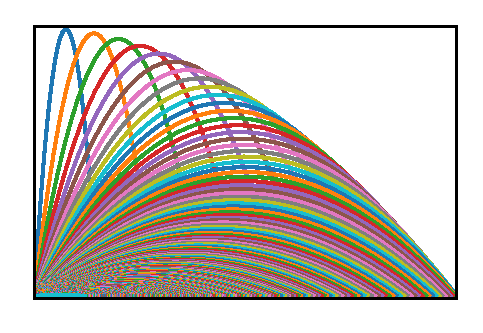
\includegraphics{trajectories}};
 \node[left] at (-3.5,2.25) {$\frac{v_0^2}{2g}$};
 \node[below] at (-3.5,-2.25) {$0$};
 \node[below] at (3.5,-2.25) {$\frac{v_0^2}{g}$};
\end{tikzpicture}}
\par\noindent\emph{Solution:} Recall from Example \ref{exmp:minmax3} in Section
4.1 that if the object is launched at an angle $0<\theta<\frac{\pi}{2}$ with the
ground, then the height $y$ attained by the object as a function of the
horizontal distance $x$ that it travels is given by
\[
y ~=~ -\frac{gx^2}{2v_0^2 \cos^2\,\theta} ~+~ x\tan\,\theta ~.
\]
The curve is a parabola, with the figure on the right showing these
parabolic trajectories for 500 values of the angle $\theta$. Clearly each
parabola intersects at least one other.The maximum
horizontal distance $\frac{v_0^2}{g}$ occurs only for $\theta=\frac{\pi}{4}$, as
was shown in Example \ref{exmp:minmax3}. The maximum vertical height
$\frac{v_0^2}{2g}$ is attained when the object is launched straight up (i.e.
$\theta = \frac{\pi}{2}$), as was shown in Exercise \ref{exer:projmax0} in
Section 5.1. By symmetry only the angles $0<\theta\le\frac{\pi}{2}$ in the same
vertical plane need be considered. So in the above figure, imagine if the
trajectories for all possible angles were included, filling up a region that
does appear to have a parabolic boundary. This will now be shown to be true.

First, it turns out that all the parabolas for $0<\theta<\frac{\pi}{2}$ have the
same directrix $y=\frac{v_0^2}{2g}$. To see why, recall from Exercise
\ref{exer:projmaxangle} in Section 4.1 that the maximum height reached by the
object is $\frac{v_0^2\,\sin^2 \theta}{2g}$, which is thus the $y$-coordinate of
the vertex of the parabola. That vertex is midway between the focus and the
directrix. The parabola is of the form $4py = x^2 + bx$, where $b$ is a constant
that does not affect the distance between the vertex and directrix\footnote{This
will be discussed further in Section 7.4.}, and $4p$ is a constant with $p<0$
such that the directrix is $-p$ units above the vertex (since $p<0$), just as in
the case $4py=x^2$. The equation of the parabola then shows that
\[
\frac{1}{4p} ~=~ -\frac{g}{2v_0^2 \cos^2\,\theta} \quad\Rightarrow\quad
p ~=~ -\frac{v_0^2 \cos^2\,\theta}{2g}
\]
so that the directrix is at
\begin{align*}
y ~&=~ \text{$y$-coordinate of the vertex} ~+~ (-p)\\
&=~ \frac{v_0^2\,\sin^2 \theta}{2g} ~+~ -\left(-\frac{v_0^2 \cos^2\,\theta}{2g}\right) ~=~
\frac{v_0^2}{2g}(\sin^2 \theta ~+~ \cos^2\,\theta)\\
y ~&=~ \frac{v_0^2}{2g}
\end{align*}
It is perhaps surprising that all the parabolic trajectories share the same
directrix $y=\frac{v_0^2}{2g}$, which is independent of the angle $\theta$. Note
that the heights of each vertex $\left(\frac{v_0^2\,\sin^2 \theta}{2g}\right)$
and focus $\left(\frac{v_0^2}{2g}(\sin^2 \theta - \cos^2\,\theta)\right)$
\emph{do} depend on $\theta$. The common directrix is the key to the remainder
of the proof.
\newpage
\noindent Now let $P$ be a point in the first quadrant of the $xy$-plane below
the common directrix $y=\frac{v_0^2}{2g}$, denoted by $D$. Then $P$ can be
either inside, outside, or on the envelope, as in Figure \ref{fig:envelope3}:

\begin{figure}[ht]
 \centering
 \subfloat[][\enskip Inside the envelope]{
 \begin{tikzpicture}[>=latex,every node/.style={font=\small}]
  \filldraw[fill=fillcolor,dashed] (0,1.6) parabola (3.2,0) -- (0,0) -- cycle;
  \draw[line width=1pt] (0,1.6) -- (3.2,1.6) node[right] {$D$};
  \draw[<->,black!60,line width=1pt] (0,2.2) node[right] {$y$} |- (3.6,0) node[right] {$x$};
  \fill (2,0.7) circle (2.5pt);
  \node[below] at (2,0.7) {$P$};
  \node[below] at (0,0) {$O$};
  \node[left] at (-0.1,1.6) {$\frac{v_0^2}{2g}$};
  \node[below] at (3.2,-0.1) {$v_0^2/g$};
 \end{tikzpicture}}
 \quad
 \subfloat[][\enskip Outside the envelope]{
 \begin{tikzpicture}[>=latex,every node/.style={font=\small}]
  \filldraw[fill=fillcolor,dashed] (0,1.6) parabola (3.2,0) -- (0,0) -- cycle;
  \draw[line width=1pt] (0,1.6) -- (3.2,1.6) node[right] {$D$};
  \draw[<->,black!60,line width=1pt] (0,2.2) node[right] {$y$} |- (3.6,0) node[right] {$x$};
  \fill (2.8,1) circle (2.5pt);
  \node[below] at (2.8,1) {$P$};
  \node[below] at (0,0) {$O$};
  \node[left] at (-0.1,1.6) {$\frac{v_0^2}{2g}$};
  \node[below] at (3.2,-0.1) {$v_0^2/g$};
 \end{tikzpicture}}
 \quad
 \subfloat[][\enskip On the envelope]{
 \begin{tikzpicture}[>=latex,every node/.style={font=\small}]
  \filldraw[fill=fillcolor,dashed] (0,1.6) parabola (3.2,0) -- (0,0) -- cycle;
  \draw[line width=1pt] (0,1.6) -- (3.2,1.6) node[right] {$D$};
  \draw[<->,black!60,line width=1pt] (0,2.2) node[right] {$y$} |- (3.6,0) node[right] {$x$};
  \fill (1.96,1) circle (2.5pt);
  \node[above right] at (1.96,1) {$P$};
  \node[below] at (0,0) {$O$};
  \node[left] at (-0.1,1.6) {$\frac{v_0^2}{2g}$};
  \node[below] at (3.2,-0.1) {$v_0^2/g$};
 \end{tikzpicture}}
 \caption[]{\enskip Trajectory envelope and a point $P$}
 \label{fig:envelope3}
\end{figure}

\noindent The origin $O=(0,0)$ is on each trajectory, so by definition
of a parabola the foci for all the trajectories must be a distance
$\frac{v_0^2}{2g}$ from $O$, i.e. the distance from $O$ to $D$. That is, the
foci of all the trajectories must lie on the circle $C_0$ of radius
$\frac{v_0^2}{2g}$ centered at $O$. If $P$ is any other point inside the
envelope, so that it lies on at least one trajectory, then it must be a distance
$r>0$ below the line $D$. By definition of a parabola, $P$ must be the same
distance from the foci of any trajectories it belongs to. That is, the foci must
be on a circle $C$ of radius $r$ centered at $P$ and touching the directrix $D$,
as in Figure \ref{fig:envfoci3}:

\begin{figure}[ht]
 \centering
 \subfloat[][\enskip Two intersections $F_1$, $F_2$]{
 \begin{tikzpicture}[>=latex,every node/.style={font=\small}]
  \filldraw[fill=fillcolor,dashed] (0,1.6) parabola (3.2,0) -- (0,0) -- cycle;
  \draw[line width=1pt] (0,1.6) -- (3.2,1.6) node[right] {$D$};
  \draw[name path=C0] (0,1.6) arc (90:-10:1.6);
  \draw[<->,black!60,line width=1pt] (0,2.2) node[right] {$y$} |- (3.6,0) node[right] {$x$};
  \fill (2,0.7) circle (2.5pt);
  \node[below] at (2,0.7) {$P$};
  \draw[name path=C] (2,0.7) circle (0.9);
  \node[below] at (0,0) {$O$};
  \node[left] at (-0.1,1.6) {$\frac{v_0^2}{2g}$};
  \node[below] at (3.2,-0.1) {$v_0^2/g$};
  \node[right] at (3,0.7) {$C$};
  \fill[name intersections={of=C and C0,by={{F1,F2}}}] (F1) circle (2.5pt) (F2) circle (2.5pt);
  \node[below left] at (F1) {$F_1$};
  \node[below left] at (F2) {$F_2$};
  \node[below right] at (0.2,1.5) {$C_0$};
  \draw[dashed] (2,0.7) -- (2,1.6) node[pos=0.7,right] {$r$};
 \end{tikzpicture}}
 \quad
 \subfloat[][\enskip No intersections]{
 \begin{tikzpicture}[>=latex,every node/.style={font=\small}]
  \filldraw[fill=fillcolor,dashed] (0,1.6) parabola (3.2,0) -- (0,0) -- cycle;
  \draw[line width=1pt] (0,1.6) -- (3.2,1.6) node[right] {$D$};
  \draw (0,1.6) arc (90:-10:1.6);
  \draw[<->,black!60,line width=1pt] (0,2.2) node[right] {$y$} |- (3.6,0) node[right] {$x$};
  \fill (2.8,1) circle (2.5pt);
  \node[below] at (2.8,1) {$P$};
  \draw (2.8,1) circle (0.6);
  \node[below] at (0,0) {$O$};
  \node[left] at (-0.1,1.6) {$\frac{v_0^2}{2g}$};
  \node[below] at (3.2,-0.1) {$v_0^2/g$};
  \node[below right] at (0.2,1.5) {$C_0$};
  \node[right] at (3.4,1) {$C$};
  \draw[dashed] (2.8,1) -- (2.8,1.6) node[midway,right] {$r$};
 \end{tikzpicture}}
 \quad
 \subfloat[][\enskip One intersection $F$]{
 \begin{tikzpicture}[>=latex,every node/.style={font=\small}]
  \filldraw[fill=fillcolor,dashed] (0,1.6) parabola (3.2,0) -- (0,0) -- cycle;
  \draw[line width=1pt] (0,1.6) -- (3.2,1.6) node[right] {$D$};
  \draw[name path=C0] (0,1.6) arc (90:-10:1.6);
  \draw[<->,black!60,line width=1pt] (0,2.2) node[right] {$y$} |- (3.6,0) node[right] {$x$};
  \fill (1.96,1) circle (2.5pt);
  \node[below] at (1.96,1) {$P$};
  \draw[name path=C] (1.96,1) circle (0.6);
  \fill[name intersections={of=C and C0,by=F}] (F) circle (2.5pt);
  \node[below left] at (F) {$F$};
  \node[below] at (0,0) {$O$};
  \node[left] at (-0.1,1.6) {$\frac{v_0^2}{2g}$};
  \node[below] at (3.2,-0.1) {$v_0^2/g$};
  \node[below right] at (0.2,1.5) {$C_0$};
  \node[right] at (2.56,1) {$C$};
  \draw[dashed] (1.96,1) -- (1.96,1.6) node[midway,right] {$r$};
 \end{tikzpicture}}
 \caption[]{\enskip Circles $C$ and $C_0$ intersect at foci of trajectories}
 \label{fig:envfoci3}
\end{figure}

\parpic[r]{ \begin{tikzpicture}[>=latex,every node/.style={font=\small}]
  \filldraw[linecolor,fill=fillcolor,line width=1pt] (0,1.6) parabola (3.2,0) -- (0,0) -- cycle;
  \draw[line width=1pt] (0,3.2) -- (3.2,3.2) node[right] {$L$};
  \draw[line width=1pt] (0,1.6) -- (3.2,1.6) node[right] {$D$};
  \draw[name path=C0,dashed] (0,1.6) arc (90:0:1.6);
  \draw[<->,black!60,line width=1pt] (0,3.8) node[right] {$y$} |- (3.6,0) node[right] {$x$};
  \fill (1.96,1) circle (2.5pt);
  \node[below] at (1.96,1) {$P$};
  \draw[name path=C,dashed] (1.96,1) circle (0.6);
  \draw[dashed] (0,0) -- (1.96,1);
  \node[below] at (0,0) {$O$};
  \node[left] at (-0.1,1.6) {$\frac{v_0^2}{2g}$};
  \node[left] at (-0.1,3.2) {$\frac{v_0^2}{g}$};
  \node[below] at (3.2,-0.1) {$v_0^2/g$};
  \draw[dashed] (1.96,1) -- (1.96,1.6) node[midway,right] {$r$};
  \draw[dashed] (1.96,1.6) -- (1.96,3.2) node[midway,right] {$\frac{v_0^2}{2g}$};
 \end{tikzpicture}}
\noindent In Figure \ref{fig:envfoci3}(a) $C$ and $C_0$ intersect at two points
$F_1$ and $F_2$, so $P$ belongs to two trajectories; $P$ must then be
\emph{inside} the envelope. In Figure \ref{fig:envfoci3}(b) $C$ and $C_0$ do not
intersect, so $P$ must be \emph{outside} the envelope (since it is not
on a parabola with a focus on $C_0$). If $C$ and $C_0$ intersect at only
one point $F$, as in Figure \ref{fig:envfoci3}(c), then $P$ must be \emph{on}
the envelope. In that case, $P$ is a distance $r+\frac{v_0^2}{2g}$ from $O$,
which is also the distance from $P$ to the line $y=\frac{v_0^2}{g}$ (denoted by
$L$). Thus, by definition of a parabola, $P$ is on a parabola with focus $O$ and
directrix $L$. The vertex is at
$\left(0,\frac{v_0^2}{2g}\right)$. Therefore, the envelope is a parabola: the
boundary of the shaded region in the figure on the right.$\quad\checkmark$
\end{exmp}
\divider
\newpage
In Example \ref{exmp:parabenvelope} all the trajectories were in the $xy$-plane
only. Removing that restriction, so that trajectories in all vertical planes
through the $y$-axis are possible, would result in a solid paraboloid
consisting of all possible trajectories from the origin.
\parpic[r]{\begin{tikzpicture}[>=latex,every node/.style={font=\small}]
 \draw[line width=2pt] (-1.55,0) -- (1.55,0);
 \foreach \x in {-1.5,-1.3,...,1.5} \draw (\x,0) -- (\x,1.5);
 \filldraw[linecolor,fill=white,line width=1.5pt] (-1.5,1.5) parabola bend (0,0.5) (1.5,1.5);
\end{tikzpicture}}
Parabolas also appear in suspension bridges: the suspension cables supporting a
horizontal bridge (via vertical suspenders, as in the figure on the right) have
to be parabolas if the weight of the bridge is uniformly
distributed.\footnote{See pp.159-161 in \textsc{Smith, C.E.}, \emph{Applied
Mechanics: Statics}, New York: John Wiley \& Sons, Inc., 1976.}\vspace{2mm}

\divider
\vspace{2mm}
\startexercises\label{sec7dot2}
{\small
\probs{A}
\begin{enumerate}[\bfseries 1.]
 \item Construct a parabola using the procedure shown in Figure
  \ref{fig:paraboladraw}.
\suspend{enumerate}
\par\noindent For Exercises 2-6, sketch the graph of the given parabola and
indicate the exact locations of the focus, vertex, and directrix.
\resume{enumerate}[{[\bfseries 1.]}]
\begin{multicols}{5}
 \item $8y=x^2$
 \item $y=8x^2$
 \item $x=y^2$
 \item $x=-3y^2$
 \item $-1000y=x^2$
\end{multicols}
 \item Find the points of intersection of the parabolas $4py=x^2$ and $4px=y^2$
  when $p>0$. What is the equation of the line through those points?
 \item A vehicle headlight in the shape of a paraboloid is 3in deep and has an
  open edge with diameter 8in. Where should the center of the bulb be placed in
  order to be at the focus, measured in inches relative to the vertex?
 \item The \emph{latus rectum}\index{parabola!latus rectum} of a parabola is the
  chord that passes through the focus and is parallel to the directrix. Find the
  length of the latus rectum for the parabola $4py=x^2$.\index{latus rectum!of parabola}
 \item Show that the circle whose diameter is the latus rectum of a parabola
  touches the parabola's directrix at one point.
 \item Find the points on the parabola $4px=y^2$ such that the focal radii to
  those points have the same length as the latus rectum.
 \item From each end of the latus rectum of a parabola draw a line to the point
  where the directrix and axis intersect. Show that the two drawn lines are
  perpendicular.
\suspend{enumerate}
\probs{B}
\resume{enumerate}[{[\bfseries 1.]}]
 \item Show that any point not on a parabola is on either zero or two tangent
  lines to the parabola.
 \item Show that $y=mx-2mp-m^3p$ is the normal line of slope $m$ to the parabola
  $4px=y^2$.
 \item From a point $P$ on a parabola with vertex $V$ let $\overline{PQ}$ be the
  line segment perpendicular to the axis at a point $Q$. Show that $PQ^2$ equals
  the product of $QV$ and the length of the latus rectum.
 \item Show that the curve $y=ax^2+bx+c$ is a parabola for $a \ne 0$, using only
  the definition of a parabola. Find the focus, vertex and directrix.
 \item Show that the set of all midpoints of a family of parallel chords in a
  parabola lie on a line parallel to the parabola's axis.
\end{enumerate}
}
\newpage
%Begin Section 7.3
\section{Hyperbolas}
In the previous two sections you have seen curves with eccentricity $e=0$
(circles), $0<e<1$ (ellipses) and $e=1$ (parabolas). The remaining case
is $e>1$: the \textbf{hyperbola}, whose definition is similar to the second
definition of the ellipse.\index{hyperbola}\index{hyperbola!definition}

\statedefn{defn:hyperbola}{A \textbf{hyperbola} is the set of all points in a
plane such that the ratio of the distance from a fixed point (a \textbf{focus})
to the distance from a fixed line (a \textbf{directrix}) is a constant $e>1$,
called the \textbf{eccentricity} of the hyperbola.}\index{hyperbola!directrix}

\piccaption[]{\label{fig:hyper1x}}\parpic[r]{\begin{tikzpicture}[>=latex,every node/.style={font=\small}]
  \begin{scope}[color=linecolor,line width=1.5pt]
   \draw[black!60,line width=1pt,->] (-1.5,0) -- (1.7,0) node[right] {$x$};
   \draw[black!60,line width=1pt,->] (0,-1.4) -- (0,1.7) node[above] {$y$};
   \pgfplothandlerlineto
   \pgfplotfunction{\x}{0.09,0.095,...,1.3}{\pgfpointxy{\x}{0.12 / \x}}
   \pgfplotfunction{\x}{-1.3,-1.295,...,-0.09}{\pgfpointxy{\x}{0.12 / \x}}
   \pgfusepath{stroke}
   \node[black,below right] at (0,0) {$0$};
   \node [black] at (1.1,1.1) {$y = \frac{1}{x}$};
  \end{scope}
 \end{tikzpicture}}
It will be shown in Section 7.4 that the curve $y=\frac{1}{x}$ is a hyperbola,
which has two branches (see Figure \ref{fig:hyper1x}). In general a
hyperbola resembles a ``wider'' or less ``cupped'' parabola, and it has two
symmetric branches (and hence two foci and two directrices) as well as two
asymptotes.

The ratio of distances referred to in the definition of the hyperbola also
appears in the second definition of the ellipse (where the ratio is smaller than
1) and in the definition of the parabola (where the ratio equals 1). In all
three cases that ratio is the eccentricity. See Figure \ref{fig:ecccompare}(a)
for the comparisons.\index{hyperbola!focus}\index{hyperbola!eccentricity}

\begin{figure}[ht]
 \centering
 \subfloat[][\enskip Eccentricity $e$]{
 \begin{tikzpicture}[>=latex,every node/.style={font=\small}]
  \draw[rotate=-90,line width=1.5pt,linecolor] (-2,3.5) parabola bend (0,0) (2,3.5);
  \draw[line width=1.5pt,linecolor] (1.5,0) ellipse (1 and 0.5);
  \draw[line width=1.5pt,linecolor] (0.75,2) to[out=210,in=90] (-0.5,0)
   to[out=-90,in=150] (0.75,-2);
  \fill (1,0) circle (2.5pt);
  \node[right] at (1,0) {$F$};
  \node[right] at (2.55,0) {$e<1$};
  \node[below left] at (3.5,1.7) {$e=1$};
  \node[right] at (0.75,2) {$e>1$};
  \draw[line width=1pt] (-1,-2.2) -- (-1,2.2) node[pos=0.7,fill=white] {$D$};
 \end{tikzpicture}}
 \qquad\qquad\qquad
 \subfloat[][\enskip Orbit velocity $v$ and escape velocity $v_E$]{
 \begin{tikzpicture}[>=latex,every node/.style={font=\small}]
  \draw[rotate=-90,line width=1.5pt,linecolor] (-2,3.5) parabola bend (0,0) (2,3.5);
  \draw[line width=1.5pt,linecolor] (1.5,0) ellipse (1 and 0.5);
  \draw[line width=1.5pt,linecolor] (0.75,2) to[out=210,in=90] (-0.5,0)
   to[out=-90,in=150] (0.75,-2);
  \fill (1,0) circle (2.5pt);
  \node[right] at (1,0) {Sun};
  \node[right] at (2.55,0) {$v<v_E$};
  \node[below left] at (3.5,1.7) {$v=v_E$};
  \node[right] at (0.75,2) {$v>v_E$};
  \draw[line width=1pt] (-1,-2.2) -- (-1,2.2) node[pos=0.7,fill=white] {$D$};
  \path(-2,0) -- (4.5,0);
 \end{tikzpicture}}
 \caption[]{\enskip Hyperbola, parabola and ellipse with focus $F$ and directrix $D$}
 \label{fig:ecccompare}
\end{figure}

There is an analogue for Figure \ref{fig:ecccompare}(a) in terms of orbits. For
example, an object approaching the Sun must meet or exceed the \textbf{escape
velocity}\index{escape velocity} to overcome the Sun's gravitational pull and
avoid returning to orbit. Figure \ref{fig:ecccompare}(b) shows the three
possible trajectories---hyperbola, parabola and ellipse---in terms of the
object's velocity $v$ and the escape velocity $v_E$. Note the apparent
correlation between the eccentricity of the object's path and its speed as a
fraction of the escape velocity (i.e. $\frac{v}{v_E}$).
\newpage
\piccaption[]{\label{fig:hyperbolavert}\enskip Hyperbola: $\frac{PF}{PG}=e>1$}\parpic[r]{\begin{tikzpicture}[every node/.style={font=\small}]
 \fill (0,0.5) circle (2.5pt);
 \draw[dashed] (0,0.5) -- (-1.6,0.64) -- (-1.6,-0.2);
 \draw[linecolor,line width=1.5pt] (-2,1) parabola bend (0,0) (2,1);
 \draw[line width=1pt] (-2.5,-0.2) -- (2.3,-0.2);
 \node[right] at (2.3,-0.2) {$D$};
 \node[above] at (0,0.5) {$F$};
 \fill (-1.6,0.64) circle (2.5pt);
 \node[left] at (-1.6,0.6) {$P$};
 \fill (-1.6,-0.2) circle (2.5pt);
 \node[below] at (-1.5,-0.2) {$G$};
 \path (-2.7,0) -- (2.7,0);
\end{tikzpicture}}
Figure \ref{fig:hyperbolavert} illustrates the definition of a hyperbola,
consisting of points $P$ whose distance $PF$ from the focus $F$ exceeds the
distance $PG$ to the directrix $D$ in a way so that the ratio $\frac{PF}{PG}$ is
always the same constant $e>1$ (the eccentricity).

\piccaption[]{\label{fig:hypereqn}}\parpic[r]{\begin{tikzpicture}[>=latex,every node/.style={font=\small}]
 \draw[black!60,line width=1pt,->] (-1,0) -- (3.5,0) node[right] {$x$};
 \draw[black!60,line width=1pt,->] (-0.1,-2) -- (-0.1,2) node[above] {$y$};
 \draw[name path=hyper,line width=1.5pt,linecolor] (2.25,2) to[out=210,in=90] (1,0)
  to[out=-90,in=150] (2.25,-2);
 \fill (2.5,0) circle (2.5pt);
 \node[below] at (2.5,-0.1) {$(ea,0)$};
 \draw[line width=1pt] (0.5,-2) -- (0.5,2.) node[pos=0.3,fill=white] {$x=\frac{a}{e}$};
 \path[name path=d2] (0.5,1.5) -- (2,1.5);
 \draw[name intersections={of=d2 and hyper,by=P}] (0.5,1.5) -- (P) node[midway,above] {$d_2$}
   -- (2.5,0) node[midway,right] {$d_1$};
 \fill (P) circle (2.5pt);
 \node[below left] at (-0.1,0) {$0$};
 \node[right] at (P) {$~(x,y)$};
 \end{tikzpicture}}
To derive the equation of a hyperbola with eccentricity $e>1$, assume the focus
is on the $x$-axis at $(ea,0)$, with $a>0$, and the line $x=\frac{a}{e}$ is the
directrix, as in Figure \ref{fig:hypereqn}. Pick a point $(x,y)$ whose distances
$d_1$ and $d_2$ from the focus $(ea,0)$ and directrix $x=\frac{a}{e}$,
respectively, satisfy the condition for a hyperbola:\\$\frac{d_1}{d_2}=e>1$.
Then
\begin{align*}
d_1^2 ~&=~ e^2 d_2^2\\
(x-ea)^2 ~+~ (y-0)^2 ~&=~ e^2\,\left(\left(x-\frac{a}{e}\right)^2 ~+~ (y-y)^2\right)\\
x^2 ~-~ \cancel{2eax} ~+~ e^2a^2 ~+~ y^2 ~&=~ e^2x^2 ~-~ \cancel{2eax} ~+~ a^2\\[4pt]
(e^2 - 1)\,x^2 ~-~ y^2 ~&=~ (e^2 - 1)\,a^2\\
%\frac{x^2}{a^2} ~-~ \frac{y^2}{(e^2 - 1)\,a^2} ~&=~ 1\\[4pt]
\frac{x^2}{a^2} ~-~ \frac{y^2}{b^2} ~&=~ 1
\end{align*}\vspace{-8mm}
\picskip{0}
\noindent where $b^2 = (e^2 - 1)\,a^2 > 0$. The
hyperbola thus has two branches ($x=\pm \frac{a}{b}\sqrt{y^2 + b^2}$), as
in Figure \ref{fig:hyperparts}. Let $c=ea$, so that $c>a$ and $b^2 = c^2-a^2$.
By symmetry the hyperbola has two foci $(\pm c,0)$ and two directrices
$x=\pm\frac{a^2}{c}$, and the lines $y=\pm \frac{b}{a}x$ are
asymptotes.\index{hyperbola!asymptotes}
The \textbf{vertexes}\index{hyperbola!vertex} are the points on the
hyperbola closest to the directrices.
\begin{figure}[h]
 \centering
 \begin{tikzpicture}[>=latex,every node/.style={font=\small}]
  \draw[black!60,line width=1pt,->] (-5.5,0) -- (5.5,0) node[right] {$x$};
  \draw[black!60,line width=1pt,->] (0,-2) -- (0,2.1) node[above] {$y$};
  \draw[line width=1.5pt,linecolor] (4.25,2) to[out=210,in=90] (3,0)
   to[out=-90,in=150] (4.25,-2);
  \fill (4.5,0) circle (2.5pt);
  \draw[line width=1.5pt,linecolor] (-4.25,2) to[out=-30,in=90] (-3,0)
   to[out=-90,in=30] (-4.25,-2);
  \fill (-4.5,0) circle (2.5pt);
  \node[below,align=center] at (4.5,-0.1) {$(c,0)$\\focus};
  \node[above right] at (3,0.1) {vertex};
  \node[below,align=center] at (-4.5,-0.1) {$(-c,0)$\\focus};
  \node[above left] at (-3,0.1) {vertex};
  \draw[line width=1pt] (2.5,-2) -- (2.5,2);
  \draw[line width=1pt] (-2.5,-2) -- (-2.5,2);
  \node[below left] at (0.1,0) {$0$};
  \node[below left] at (2.5,0) {$\frac{a^2}{c}$};
  \node[below right] at (-2.5,0) {$-\frac{a^2}{c}$};
  \node[below right] at (3,0) {$a$};
  \node[below left] at (-3,0) {$-a$};
  \fill (3,0) circle (2.5pt);
  \fill (-3,0) circle (2.5pt);
  \draw[dashed] (-4,-2.1) -- (4,2.1) node[pos=0.75,above left,align=center]
   {asymptote\\$y=\frac{b}{a}x$};
  \draw[dashed] (-4,2.1) -- (4,-2.1) node[pos=0.25,above right,align=center]
   {asymptote\\$y=-\frac{b}{a}x$};
  \node[align=left,above right] at (0,-2) {conjugate\\axis};
  \node[align=right,above left] at (-5.5,0) {transverse\\axis};
  \node[above] at (-2.5,2) {directrix};
  \node[above] at (2.5,2) {directrix};
 \end{tikzpicture}
 \caption[]{\enskip Parts of the hyperbola $\frac{x^2}{a^2} - \frac{y^2}{b^2} = 1$,
  with $b^2 = c^2 - a^2$}
 \label{fig:hyperparts}
\end{figure}

\noindent The \textbf{center}\index{hyperbola!center} is the point midway
between the foci. The \textbf{transverse axis}\index{transverse axis} and
\index{hyperbola!transverse axis} \textbf{conjugate axis}\index{conjugate axis}
are the perpendicular lines through the foci and center,
respectively.\index{hyperbola!conjugate axis}
\newpage
In Figure \ref{fig:hyperparts} the vertexes are $(\pm a,0)$, the $x$-axis is the
transverse axis, the center is the origin $(0,0)$, and the conjugate axis is the
$y$-axis.
Note that the existence of \emph{two} foci and directrices---when the definition
of the hyperbola mentioned only \emph{a} focus and \emph{a} directrix---is
simply a consequence of the symmetry about \emph{both} axes imposed by the
equation $\frac{x^2}{a^2} - \frac{y^2}{b^2} = 1$. A parabola, in comparison,
is symmetric about only \emph{one} axis.

To see why the lines $y=\pm \frac{b}{a}x$ are asymptotes, consider the upper
half $y=\frac{b}{a}\sqrt{x^2 - a^2}$ of both branches of the hyperbola. The
difference between the line $y=\frac{b}{a}x$ and the upper right branch
approaches zero as $x$ approaches infinity:
\begin{align*}
\lim_{x \to \infty} \,\left(\frac{b}{a}x ~-~ \frac{b}{a}\sqrt{x^2 - a^2}\right) ~&=~
 \frac{b}{a}\,\lim_{x \to \infty} \,\left(x ~-~ \sqrt{x^2 - a^2}\,\right) \,\cdot\,
 \frac{x ~+~ \sqrt{x^2 - a^2}}{x ~+~ \sqrt{x^2 - a^2}}\\[4pt]
&=~ \frac{b}{a}\,\lim_{x \to \infty} \,\frac{x^2 ~-~ (x^2 - a^2)}{x ~+~ \sqrt{x^2 - a^2}}\\[4pt]
&=~ \lim_{x \to \infty} \,\frac{ab}{x ~+~ \sqrt{x^2 - a^2}} ~=~ 0
\end{align*}
Thus the line $y=\frac{b}{a}x$ is an (oblique) asymptote for the upper half
$y=\frac{b}{a}\sqrt{x^2 - a^2}$ of the right branch in the first quadrant of
the $xy$-plane. So by symmetry the lines $y=\pm \frac{b}{a}x$ are asymptotes for
both branches, i.e. for the entire hyperbola.

Conversely, given a hyperbola in the form
$\frac{x^2}{a^2} - \frac{y^2}{b^2} = 1$, let $c^2=a^2+b^2$ to get the foci
$(\pm c,0)$ and the directrices $x=\pm\frac{a^2}{c}$, while the eccentricity is
$e = \frac{c}{a}$.

\begin{exmp}
\noindent For the hyperbola $x^2 - y^2 = 1$ find the vertexes, foci,
directrices, asymptotes and eccentricity.\vspace{1mm}
\par\noindent\emph{Solution:} Here $a=b=1$, so that $c^2=a^2+b^2=2$,
i.e. $c=\sqrt{2}$. The vertexes are thus $(\pm 1,0)$, the asymptotes are
$y=\pm x$, the foci are $(\pm\sqrt{2},0)$, the directrices are
$x=\pm\frac{1}{\sqrt{2}}$, and the eccentricity is $e=\sqrt{2}$.
\end{exmp}\vspace{-3mm}
\divider
\vspace{2mm}
\piccaption[]{\label{fig:hyperyx}\enskip $\frac{y^2}{a^2} - \frac{x^2}{b^2} = 1$}\parpic[r]{
 \begin{tikzpicture}[>=latex,every node/.style={font=\small}]
  \draw[black!60,line width=1pt,->] (-2,0) -- (2.93,0) node[right] {$x$};
  \draw[black!60,line width=1pt,->] (0,-2) -- (0,2.1) node[right] {$y$};
  \fill (0,1.6) circle (2.5pt);
  \node[left] at (-0.1,1.6) {$c$};
  \draw[linecolor,line width=1.5pt] (-2,2) parabola bend (0,1) (2,2);
  \fill (0,1) circle (2.5pt);
  \node[above left] at (0,1) {$a$};
  \draw (-2,0.7) -- (2.9,0.7) node[pos=0.95,fill=white] {$y=\frac{a^2}{c}$};
  \fill (0,-1.6) circle (2.5pt);
  \node[left] at (-0.1,-1.6) {$-c$};
  \draw[linecolor,line width=1.5pt] (-2,-2) parabola bend (0,-1) (2,-2);
  \fill (0,-1) circle (2.5pt);
  \node[below left] at (0,-1) {$-a$};
  \draw (-2,-0.7) -- (2.9,-0.7) node[pos=0.93,fill=white] {$y=-\frac{a^2}{c}$};
  \draw[dashed] (-2,-1.8) -- (2,1.8) node[below right] {$y=\frac{a}{b}x$};
  \draw[dashed] (-2,1.8) -- (2,-1.8) node[above right] {$y=-\frac{a}{b}x$};
 \end{tikzpicture}}
\noindent Switching the roles of $x$ and $y$ produces the rotated hyperbola
$\frac{y^2}{a^2} - \frac{x^2}{b^2} = 1$, shown in Figure \ref{fig:hyperyx}.
The transverse axis is the $y$-axis, the conjugate axis is the
$x$-axis, the vertexes are at $(0,\pm a)$, and the foci are at $(0,\pm c)$,
where $c^2 = a^2 + b^2$. The directrices are $y=\pm\frac{a^2}{c}$, the
asymptotes are $y=\pm\frac{a}{b}x$, and the eccentricity is $e=\frac{c}{a}$.

For example, the hyperbola $y^2 - x^2 = 1$ has $a=b=1$, so that $c=\sqrt{2}$.
The vertexes are $(0,\pm 1)$, the asymptotes are $y=\pm x$, the foci are
$(0,\pm\sqrt{2})$, the directrices are $y=\pm\frac{1}{\sqrt{2}}$, and the
eccentricity is $e=\sqrt{2}$. The hyperbola $y^2 - x^2 = 1$ is just the
hyperbola $x^2 - y^2 = 1$ rotated $90\Degrees$.

\picskip{0}
\newpage
There is another way to define a hyperbola, in terms of two foci:

\statedefn{defn:hyperaltdefn}{A \textbf{hyperbola} is the set of all points in a
plane such that the absolute value of the difference of the distances from two
fixed points (the \textbf{foci}) is a positive constant.}

Figure \ref{fig:hyperaltdefn} illustrates the above definition with foci $F_1$
and $F_2$. The difference $d_1-d_2$ of the distances $d_1$ and $d_2$ can be
positive or negative depending on which branch the point $(x,y)$ is on, which is
why the absolute value $\abs{d_1-d_2}$ is used.

\begin{figure}[h]
\begin{minipage}[b]{8cm}
 \begin{center}
  \begin{tikzpicture}[>=latex,every node/.style={font=\small}]
 \draw[black!60,line width=1pt,->] (-2.5,0) -- (3,0) node[right] {$x$};
 \draw[black!60,line width=1pt,->] (0,-2) -- (0,2) node[above] {$y$};
 \draw[name path=hyper2,line width=1.5pt,linecolor] (1.75,2) to[out=210,in=90] (0.5,0)
  to[out=-90,in=150] (1.75,-2);
 \draw[name path=hyper1,line width=1.5pt,linecolor] (-1.75,2) to[out=-30,in=90] (-0.5,0)
  to[out=-90,in=30] (-1.75,-2);
 \fill (2,0) circle (2.5pt);
 \node[below] at (2,-0.1) {$F_2$};
 \fill (-2,0) circle (2.5pt);
 \node[below] at (-2,-0.1) {$F_1$};
 \path[name path=d2] (0.5,1.5) -- (2,1.5);
 \draw[name intersections={of=d2 and hyper2,by=P}] (-2,0) -- (P) node[pos=0.75,above] {$d_1$}
   -- (2,0) node[midway,right] {$d_2$};
 \fill (P) circle (2.5pt);
 \node[below left] at (0,0) {$0$};
 \node[right] at (P) {$~(x,y)$};
  \end{tikzpicture}\vspace{-4mm}
 \end{center}
 \caption[]{\enskip Hyperbola: $\abs{d_1-d_2} = $ constant $>0$}
 \label{fig:hyperaltdefn}
\end{minipage}
\begin{minipage}[b]{7cm}
 \begin{center}
  \begin{tikzpicture}[>=latex,every node/.style={font=\small}]
  \draw[name path=hyper,line width=1pt,dashed,linecolor] (3.75,2) to[out=210,in=90] (2.5,0)
   to[out=-90,in=150] (3.75,-2);
  \node[below] at (3.8,-0.1) {$F_2$};
  \fill (0,0) circle (2.5pt);
  \node[below] at (0,-0.1) {$F_1$};
  \draw[name path=ruler,rotate=15,line width=1pt] (0,0) rectangle (5,0.2);
  \node[name intersections={of=hyper and ruler,by={{Q,P}}},shift={(0.1,-0.1)},below] at (P) {$P$};
  \draw[shift={(P)},red!60,line width=1.5pt,rotate=10] (P) -- (2.315,0.2);
  \draw[red!60,line width=1.5pt] (3.8,0) -- (P);
  \fill (P) circle (2.5pt);
  \fill (3.8,0) circle (2.5pt);
  \node[right] at (4.83,1.34) {$A$};
  \node[xshift=0.35cm,yshift=0.07cm,rotate=-143] at (P) {\smallpencil};
  \draw[->] (50:1.1) arc (30:110:0.5);
  \draw[->] (-10:0.9) arc (-10:-90:0.5);
  \node[above] at (1.8,0.7) {$L$};
  \end{tikzpicture}\vspace{-4mm}
 \end{center}
 \caption[]{\enskip Construction of a hyperbola}
 \label{fig:drawhyper}
\end{minipage}
\end{figure}\vspace{-2mm}

It is left as an exercise to show that this second definition yields the same
equation of the hyperbola as from the first definition. The second definition
is often used as the primary definition in many textbooks, perhaps because it
provides a simple way to construct a hyperbola by hand. Figure
\ref{fig:drawhyper} shows the procedure for foci $F_1$ and $F_2$: at the focus
$F_1$ fasten one end of a ruler of length $L$, and at the other end $A$ of the
ruler fasten one end of a string of length $L-d$ for some number $0<d<F_1F_2$.
Fasten the other end of the string to the focus $F_2$ and hold the string taut
with a pencil against the ruler at a point $P$, while rotating the ruler about
$F_1$. The drawn figure will be one branch of a hyperbola, since the difference
$PF_1 - PF_2$ will always be the positive constant
$d$:\index{hyperbola!construction}
\[
PF_1 - PF_2 ~=~ (L - AP) ~-~ PF_2 ~=~ L ~-~ (AP + PF_2) ~=~ L ~-~ (L - d) ~=~ d
\]
Reverse the roles of $F_1$ and $F_2$ to draw the other branch of the hyperbola.

By Exercise \ref{exer:hyptan} in Section 3.4, the tangent
line to the hyperbola $\frac{x^2}{a^2} - \frac{y^2}{b^2} = 1$ at a point
$(x_0,y_0)$ is
\begin{equation}\label{eqn:hypertan}
\frac{x x_0}{a^2} ~-~ \frac{y y_0}{b^2} = 1 ~,
\end{equation}
so that its slope is $\frac{b^2x_0}{a^2y_0}$ when $y_0 \ne 0$. Note that by the
above equation, when $y_0=0$ (so that $x_0=\pm a$) the two tangent lines are the
vertical lines $x=\pm a$.
\newpage
That slope will
be used in proving the \textbf{reflection property} for the hyperbola:
\emph{Light shone from one focus will reflect off the hyperbola in the opposite
direction from the other focus.} Figure \ref{fig:hyperreflect} shows the light's
path from focus $F_2$ as it reflects at the point $P$ along the line through
$P$ and the other focus
$F_1$.\index{reflection property!hyperbola}\index{hyperbola!reflection property}

\begin{figure}[h]
\begin{minipage}[b]{6.5cm}
 \begin{center}
  \begin{tikzpicture}[>=latex,every node/.style={font=\small},
    decoration={markings,mark=at position 0.55 with {\arrow{triangle 60}}}]
   \draw[name path=hyper2,line width=1.5pt,linecolor] (2,2) to[out=210,in=90] (0.5,0)
    to[out=-90,in=150] (2,-2);
   \draw[name path=hyper1,line width=1.5pt,linecolor] (-2,2) to[out=-30,in=90] (-0.5,0)
    to[out=-90,in=30] (-2,-2);
   \fill (2,0) circle (2.5pt);
   \node[below] at (2,-0.1) {$F_2$};
   \fill (-2,0) circle (2.5pt);
   \node[below] at (-2,-0.1) {$F_1$};
   \path[name path=d1] (-2,0) -- (2.5,1.5);
   \draw[dashed,name intersections={of=d1 and hyper2,by=P}] (-2,0) -- (P);
   \draw[postaction={decorate}] (2,0) -- (P);
   \draw[-triangle 60,postaction={decorate}] (P) -- (2.5,1.5);
   \fill (P) circle (2.5pt);
   \node[above left] at (P) {$P$};
  \end{tikzpicture}\vspace{-4mm}
 \end{center}
 \caption[]{\enskip Reflection property}
 \label{fig:hyperreflect}
\end{minipage}
\begin{minipage}[b]{8.5cm}
 \begin{center}
  \begin{tikzpicture}[>=latex,every node/.style={font=\small},
   extended line/.style={shorten >=-#1,shorten <=-#1}]
   \draw[shift={(2,0)}] (-0.8,0) arc (180:144:0.8);
   \draw[shift={(-2,0)}] (1.15,0) arc (0:18.5:1.15);
   \draw[shift={(0.25,0)}] (0:0.5) arc (0:62:0.5);
   \draw[black!60,line width=1pt,->] (-2.5,0) -- (3,0) node[right] {$x$};
   \draw[black!60,line width=1pt,->] (0,-2) -- (0,2) node[above] {$y$};
   \draw[name path=hyper2,line width=1.5pt,linecolor] (2,2) to[out=210,in=90] (0.5,0)
    to[out=-90,in=150] (2,-2);
   \draw[name path=hyper1,line width=1.5pt,linecolor] (-2,2) to[out=-30,in=90] (-0.5,0)
    to[out=-90,in=30] (-2,-2);
   \fill (2,0) circle (2.5pt);
   \node[above] at (2,0.1) {$F_2$};
   \node[below] at (2,-0.1) {$(c,0)$};
   \fill (-2,0) circle (2.5pt);
   \node[above] at (-2,0.1) {$F_1$};
   \node[below] at (-2,-0.1) {$(-c,0)$};
   \path[name path=d1] (-2,0) -- (2.5,1.5);
   \draw[dashed,name intersections={of=d1 and hyper2,by=P}] (-2,0) -- (P);
   \draw (2,0) -- (P);
   \draw (P) -- (2.5,1.5);
   \fill (P) circle (2.5pt);
   \node[above left,align=right] at (P) {$P$\\$(x_0,y_0)$};
   \node at (-1.1,0.15) {$\alpha_1$};
   \node at (1.5,0.15) {$\alpha_2$};
   \draw[extended line=1cm] (0.25,0) -- (P);
   \node[above] at (1.2,1.8) {$L$};
   \node[below,xshift=0.1cm] at (P) {$\theta_1$};
   \node[above right,xshift=0.22cm,yshift=0.12cm] at (P) {$\theta_2$};
   \node[below left,xshift=-0.15cm,yshift=-0.1cm] at (P) {$\theta_2$};
   \node at (0.62,0.15) {$\theta$};
   \draw[shift={(P)}] (18.5:0.8) arc (18.5:62:0.8);
   \draw[shift={(P)}] (198.5:0.75) arc (198.5:242:0.75);
   \draw[shift={(P)}] (242:0.47) arc (242:324:0.47);
   \draw[shift={(0.25,0)}] (10:0.5) arc (10:62:0.5);
   \node[below] at (0.25,-0.1) {$A$};
  \end{tikzpicture}\vspace{-4mm}
 \end{center}
 \caption[]{\enskip Hyperbola $\frac{x^2}{a^2} - \frac{y^2}{b^2} = 1$ with foci $(\pm c,0)$}
 \label{fig:hyperreflpt1}
\end{minipage}
\end{figure}\vspace{-2mm}
By Fermat's Principle for curved surfaces, the reflection property is equivalent
to saying the tangent line $L$ to the hyperbola at the point $P=(x_0,y_0)$
bisects the angle $\angle F_1PF_2$, i.e. $\theta_1=\theta_2$ as in Figure
\ref{fig:hyperreflpt1}. The reflection property holds trivially when $y_0=0$
(the light reflects straight back along the $x$-axis), so to show that
$\theta_1=\theta_2$ assume $y_0 \ne 0$. By symmetry only $x_0 > 0$ need be
considered. For the case $x_0 \ne c$, let $A$ be the $x$-intercept of the
tangent line $L$. Then by Figure \ref{fig:hyperreflpt1}, since the sum of the
angles in the triangle $\triangle F_1PA$ equals $180\Degrees$,
\[
\alpha_1 + \theta_2 + (180\Degrees -\theta) = 180\Degrees \quad\Rightarrow\quad
\theta_2 = \theta - \alpha_1 \quad\Rightarrow\quad
\tan\,\theta_2 ~=~ \tan\,(\theta - \alpha_1) ~.
\]
Thus, since $\tan\,\theta$ is the slope of the tangent line $L$ (i.e.
$\frac{b^2x_0}{a^2y_0}$), and $\tan\,\alpha_1 = \frac{y_0}{x_0 + c}$, then by
the subtraction formula for the tangent function
\begin{align*}
\tan\,\theta_2 ~&=~ \frac{\tan\,\theta ~-~ \tan\,\alpha_1}{1 ~+~ \tan\,\theta\;\tan\,\alpha_1} ~=~
 \frac{\frac{b^2x_0}{a^2y_0} ~-~ \frac{y_0}{x_0 ~+~ c}}{1 ~+~
 \frac{b^2x_0}{a^2y_0}\;\cdot\;\frac{y_0}{x_0 ~+~ c}} ~=~
 \frac{\frac{b^2 x_0^2 ~-~ a^2 y_0^2 ~+~ b^2 x_0 c}{\cancel{a^2 y_0\,(x_0 ~+~
  c)}}}{\frac{(a^2 ~+~ b^2)\,x_0 y_0 ~+~ a^2 y_0 c}{\cancel{a^2 y_0\,(x_0 ~+~ c)}}}\\[6pt]
&=~ \frac{a^2 b^2 + b^2 x_0 c}{c^2 x_0 y_0 + a^2 y_0 c}
 \quad\text{(since $c^2 = a^2 + b^2$, and $\tfrac{x_0^2}{a^2} - \tfrac{y_0^2}{b^2} = 1 ~\Rightarrow~
  b^2 x_0^2 ~-~ a^2 y_0^2 = a^2 b^2$)}\\[6pt]
&=~ \frac{b^2 \,\cancel{(a^2 ~+~ x_0 c)}}{cy_0\,\cancel{(a^2 ~+~ x_0 c)}} ~=~ \frac{b^2}{cy_0}
\end{align*}
Similarly, since the sum of the angles in the triangle
$\triangle F_2PA$ equals $180\Degrees$,
\[
\alpha_2 + \theta_1 + \theta = 180\Degrees \quad\Rightarrow\quad
\theta_1 = 180\Degrees - (\theta + \alpha_2) \quad\Rightarrow\quad
\tan\,\theta_1 ~=~ -\tan\,(\theta + \alpha_2) ~.
\]
\newpage
\noindent Thus, since $\tan\,\alpha_2 = -\tan\,(180\Degrees - \alpha_2) =
-\frac{y_0}{x_0-c}$,
\begin{align*}
\tan\,\theta_1 ~&=~ -\frac{\tan\,\theta ~+~ \tan\,\alpha_2}{1 ~-~ \tan\,\theta\;\tan\,\alpha_2} ~=~
 -\frac{\frac{b^2x_0}{a^2y_0} ~+~ \frac{-y_0}{x_0 ~-~ c}}{1 ~-~
 \frac{b^2x_0}{a^2y_0}\;\cdot\;\frac{-y_0}{x_0 ~-~ c}} ~=~
 -\frac{\frac{b^2 x_0^2 ~-~ a^2 y_0^2 ~-~ b^2 x_0 c}{\cancel{a^2 y_0\,(x_0 ~-~
  c)}}}{\frac{(a^2 ~+~ b^2)\,x_0 y_0 ~-~ a^2 y_0 c}{\cancel{a^2 y_0\,(x_0 ~-~ c)}}}\\[6pt]
&=~ -\frac{a^2 b^2 - b^2 x_0 c}{c^2 x_0 y_0 - a^2 y_0 c} ~=~
  \frac{b^2 \,\cancel{(a^2 ~-~ x_0 c)}}{cy_0\,\cancel{(a^2 ~-~ x_0 c)}} ~=~ \frac{b^2}{cy_0}
~=~ \tan\,\theta_2 ~,
\end{align*}
i.e. $\theta_1 = \theta_2$
(since $0\Degrees < \theta_1,\,\theta_2 < 90\Degrees$). $\checkmark\quad$
Note: The case $x_0=c$ is left as an exercise.\vspace{1mm}

\divider
\vspace{2mm}

Ellipses, parabolas and hyperbolas are sometimes called
\textbf{conic sections}\index{conic sections}, due to being formed by
intersections of planes with a double circular cone of unlimited extent:

\begin{figure}[ht]
 \centering
 \subfloat[][\enskip Ellipse]{
 \begin{tikzpicture}
  \coordinate[shift={(-1.2,-0.8)}] (A) at (0,0);
  \coordinate[shift={(-1.2,-0.8)}] (B) at (69:0.7);
  \coordinate (C) at ($(B) +(2.5,-0.5)$);
  \coordinate (D) at ($(C) +(-111:0.7)$);
  \fill[fill opacity=0.6,fill=planecolor] (A) -- (B) -- (C) -- (D) -- cycle;
  \draw (B) -- (C);
  \shadedraw[left color=insideo,right color=insideo,middle color=insidei,fill opacity=0.4]
   (1.3,2) arc (0:180:1.3 and 0.5) -- (-1.3,2) arc (180:360:1.3 and 0.5);
  \shadedraw[left color=outer,right color=outer,middle color=inner,fill opacity=0.7]
   (-1.3,-2) arc (180:360:1.3 and 0.5) -- (-1.3,2) --
   (-1.3,2) arc (180:360:1.3 and 0.5) -- (-1.3,-2);
  \filldraw[fill=conicfillcolor,rotate=-12,shift={(0.2,-0.7)},fill opacity=0.5]
   (0,0) ellipse (0.46cm and 0.15cm);
  \draw (C) -- (D) -- (A) -- (B);
  \draw [dashed,line width=0.2pt] (1.275,-2) arc (0:180:1.275 and 0.5);
 \end{tikzpicture}}
 \qquad\qquad\qquad\quad
 \subfloat[][\enskip Parabola]{
 \begin{tikzpicture}[>=latex,every node/.style={font=\small}]
  \coordinate[shift={(0,-2)}] (A) at (250:1.3 and 0.5);
  \coordinate[shift={(0,-2)}] (B) at (60:1.3 and 0.5);
  \coordinate (C) at ($(B) +(-1.3,2)$);
  \coordinate (D) at ($(A) +(-1.3,2)$);
  \fill[fill opacity=0.6,fill=planecolor] (A) -- (B) -- (C) -- (D) -- cycle;
  \draw (A) -- (B) -- (C);
  \shadedraw[left color=insideo,right color=insideo,middle color=insidei,fill opacity=0.4]
   (1.3,2) arc (0:180:1.3 and 0.5) -- (-1.3,2) arc (180:360:1.3 and 0.5);
  \shadedraw[left color=outer,right color=outer,middle color=inner,fill opacity=0.7]
   (-1.3,-2) arc (180:360:1.3 and 0.5) -- (-1.3,2) --
   (-1.3,2) arc (180:360:1.3 and 0.5) -- (-1.3,-2);
  \filldraw[fill=conicfillcolor,fill opacity=0.5] (A) ..
   controls ($(D) +(0.64,-0.5)$) and ($(C) +(0.25,-0.4)$) .. (B);
  \draw (C) -- (D) -- (A);
  \draw [dashed,line width=0.2pt] (1.275,-2) arc (0:180:1.275 and 0.5);
 \end{tikzpicture}}
 \qquad\qquad\qquad\qquad
 \subfloat[][\enskip Hyperbola]{
 \begin{tikzpicture}[>=latex,every node/.style={font=\small}]
  \coordinate[shift={(0,-2)}] (A) at (210:1.3 and 0.5);
  \coordinate[shift={(0,-2)}] (B) at (100:1.3 and 0.5);
  \coordinate[shift={(0,2)}] (C) at (100:1.3 and 0.5);
  \coordinate[shift={(0,2)}] (D) at (210:1.3 and 0.5);
  \fill[fill opacity=0.6,fill=planecolor] (A) -- (B) -- (C) -- (D) -- cycle;
  \draw (A) -- (B) -- (C) -- (D);
  \shadedraw[left color=insideo,right color=insideo,middle color=insidei,fill opacity=0.4]
   (1.3,2) arc (0:180:1.3 and 0.5) -- (-1.3,2) arc (180:360:1.3 and 0.5);
  \shadedraw[left color=outer,right color=outer,middle color=inner,fill opacity=0.7]
   (-1.3,-2) arc (180:360:1.3 and 0.5) -- (-1.3,2) --
   (-1.3,2) arc (180:360:1.3 and 0.5) -- (-1.3,-2);
  \filldraw[fill=conicfillcolor,fill opacity=0.5] (A) ..
   controls ($(D) +(0.24,-2.8)$) and ($(C) +(0,-2.7)$) .. (B);
  \filldraw[fill=conicfillcolor,fill opacity=0.5] (C) ..
   controls ($(B) +(0,2.8)$) and ($(A) +(0.7,2.7)$) .. (D);
  \draw (A) -- (D);
  \draw [dashed,line width=0.2pt] (1.275,-2) arc (0:180:1.275 and 0.5);
 \end{tikzpicture}}
 \caption[]{\enskip Conic sections}
 \label{fig:conics}
\end{figure}

Each double cone in Figure \ref{fig:conics} has two\index{nappe}
\textbf{nappes}---a cone extending upward and one extending downward.
When a plane intersects only one nappe in a closed noncircular curve, as in
Figure \ref{fig:conics}(a), that curve is an ellipse. A plane that is parallel
to a line on one nappe, as in Figure \ref{fig:conics}(b), intersects only
that nappe in a parabola. The intersection of a plane with both nappes, as in
Figure \ref{fig:conics}(c), is a hyperbola.

\piccaption[]{\label{fig:spheretan}}\parpic[r]{\begin{tikzpicture}[every node/.style={font=\small}]
 \shade[ball color=spherecolor,opacity=0.5] (0,0) circle (1.25);
 \draw[line width=0.2pt] (-1.25,0) arc (180:360:1.25 and 0.3);
 \draw[dashed,line width=0.2pt] (1.25,0) arc (0:180:1.25 and 0.3);
 \fill (0,0) circle (2.5pt);
 \node[right] at (0,0) {$O$};
 \fill (135:1.25) circle (2.5pt);
 \node[above] at (135:1.25) {$P_1$};
 \fill (225:1.25) circle (2.5pt);
 \node[below] at (225:1.25) {$P_2$};
 \draw (0,0) -- (225:1.25) -- ++(135:1.25) node[left] {$Q$} -- (0,0);
 \draw (0,0) -- (135:1.25) -- ++(225:1.25);
 \draw[shift={(135:1.25)}] (225:0.2) -- ++(-45:0.2) -- ++(45:0.2);
 \draw[shift={(225:1.25)}] (45:0.2) -- ++(135:0.2) -- ++(225:0.2);
 \fill (-1.76,0) circle (2.5pt);
\end{tikzpicture}}
To prove that the ellipse, parabola and hyperbola really are represented by the
indicated conic sections, first a minor result is needed from three-dimensional
geometry: tangent line segments to a sphere from the same point have equal
lengths, as in Figure \ref{fig:spheretan}. Since the right triangles
$\triangle QOP_1$ and $\triangle QOP_2$ share the same hypotenuse
$\overline{QO}$ and have legs $\overline{OP_1}$ and $\overline{OP_2}$ of equal
length (the radius of the sphere), the result $QP_1=QP_2$ follows by the
Pythagorean Theorem.
\newpage
\piccaption[]{\label{fig:conicproof}}\parpic[r]{\begin{tikzpicture}[every node/.style={font=\small}]
 \path[clip] (-3.6,-1.2) rectangle (4.2,4.1);
 \fill[fill opacity=0.5,fill=green!30] (-3.5,0.5) -- (3,0.5) -- (4,1.5) -- (-2.5,1.5);
 \fill[fill opacity=0.5,fill=green!30] (3,0.5) -- (4,1.5) -- (-1.5,3.4) -- (-2.5,2.4);
 \shade[ball color=spherecolor,opacity=0.5] (0,0) circle (2);
 \filldraw[fill=inner,fill opacity=0.5] (3.464,-2) -- (0,4) -- (-3.464,-2);
 \draw[dashed] (3.464,-2) -- (-3.464,-2);
 \draw[shift={(0,1)}] (-1.732,0) arc (-180:0:1.732 and 0.3);
 \draw[dashed,shift={(0,1)}] (1.732,0) arc (0:180:1.732 and 0.3);
 \draw (-3.5,0.5) -- (3,0.5) -- (4,1.5) node[pos=0.8,right] {$D$} -- (-1.5,3.4)
  -- (-2.5,2.4) -- (3,0.5);
 \draw (3,0.5) -- (-3.5,0.5) -- (-2.5,1.5) -- (4,1.5);
 \draw[name path=e,fill=conicfillcolor,rotate=-15,shift={(-0.42,2.1)},fill opacity=0.5]
   (0,0) ellipse (1.08cm and 0.35cm);
 \fill (75:2) circle (2.5pt);
 \node[above] at (75:2) {$F$};
 \coordinate (Q) at (-0.6,0.7);
 \fill (Q) circle (2.5pt);
 \node[above left] at (Q) {$Q$};
 \coordinate (P) at (-0.2,1.9);
 \fill (P) circle (2.5pt);
 \node[above] at (-0.2,1.9) {$P$};
 \draw (75:2) -- (P) -- (Q);
 \coordinate (A) at (-0.2,0.8);
 \coordinate (B) at (3.3,0.8);
 \fill (B) circle (2.5pt);
 \draw[dashed] (P) -- (A) -- (B) node[right] {$G$};
 \draw (B) -- (P);
 \draw[dashed] (A) -- (Q);
 \node at (-2.1,2.45) {$P_c$};
 \node at (-3,0.67) {$P_0$};
 \node[above right] at (A) {$A$};
 \node at (2.5,0.9) {$\alpha$};
 \node[above right] at (Q) {$\beta$};
 \node[above right] at (-2.9,-1.2) {$\beta$};
 \node[above] at (-0.3,2.5) {$C$};
\end{tikzpicture}}
For the case of a right circular double cone (i.e. the base of each nappe is a
circle in a plane perpendicular to the axis of the cone\footnote{The proof can
be extended to oblique double cones. See \S 364 in \textsc{Salmon, G.S.},
\emph{A Treatise on Conic Sections}, London: Longmans, Green and Co., 1929.}),
let $\beta$ be the complement of the angle that the cone makes with its axis, as
in Figure \ref{fig:conicproof}. So $\beta$ is the angle the cone makes with any
circular base of the cone. This constant angle $\beta$, with $0\Degrees < \beta
< 90\Degrees$, is an intrinsic property of the cone. Let $P_c$ be a plane that
intersects the lower nappe of the cone in a curve $C$, such that $P_c$ makes an
angle $\alpha$ with any base circle of the cone. By symmetry, only the angles
$0\Degrees < \alpha \le 90\Degrees$ need be considered.\footnote{The case
where $\alpha = 0\Degrees$ results in a circle, which is typically not
considered a conic section.}
Inscribe a sphere in the cone so that it touches $P_c$ at a point $F$, as in
Figure \ref{fig:conicproof} ($P_c$ is the \emph{tangent plane} to the sphere at
$F$). Let $P_0$ be the plane through the circle where the inscribed sphere
touches the cone, and let $D$ be the line of intersection of the planes $P_c$
and $P_0$. It will be shown that $F$ and $D$ are the focus and directrix,
respectively, of the curve $C$.

Let $P$ be any point on the curve $C$, then let
$Q$ be the point on the plane $P_0$ that lies on a line through $P$ and the
cone's vertex. Drop a perpendicular line segment from $P$ to the point $A$ in
the plane $P_0$. From $A$ draw a perpendicular line segment to the point $G$ on
the line $D$. Then as Figure \ref{fig:conicproof} shows, $\triangle QAP$ and
$\triangle PAG$ are right triangles, with
\[
\sin\,\alpha ~=~ \frac{PA}{PG} \quad\text{and}\quad
\sin\,\beta ~=~ \frac{PA}{PQ} ~.
\]
However, since $\overline{PF}$ and $\overline{PQ}$ are both tangent line
segments to the inscribed sphere from the same point $P$, the result proved
earlier shows that $PQ = PF$. Thus,
\[
PG\,\sin\,\alpha ~=~ PA ~=~ PQ\,\sin\,\beta ~=~ PF\,\sin\,\beta
\quad\Rightarrow\quad \frac{PF}{PG} ~=~ \frac{\sin\,\alpha}{\sin\,\beta} ~.
\]
Let $e = \frac{PF}{PG}$. Then $e$ is the same constant
$\frac{\sin\,\alpha}{\sin\,\beta}$ for any point $P$ on the curve $C$. Thus, by
definition, $e$ is the eccentricity of the curve $C$ with focus $F$ and
directrix $D$. If $0\Degrees < \alpha < \beta$ then $0\Degrees <
\sin\,\alpha < \sin\,\beta$ so that $0 < \frac{\sin\,\alpha}{\sin\,\beta} < 1$,
which means that $0 < e < 1$, and hence $C$ is an ellipse (by the second
definition of an ellipse). Likewise, if $\alpha = \beta$ then $e=1$, so that $C$
is a parabola. Finally, if $\beta < \alpha \le 90\Degrees$ then $e > 1$, so that
$C$ is a hyperbola (and will intersect both nappes of the cone). Thus, the
ellipse, parabola and hyperbola truly are conic sections. $\checkmark$
\newpage
\startexercises\label{sec7dot3}
{\small
\probs{A}
\begin{enumerate}[\bfseries 1.]
 \item Construct a hyperbola using the procedure shown in Figure
  \ref{fig:drawhyper}. Place the two focus pins 7in apart and use a 9in piece of
  string attached to a 12in ruler.
\suspend{enumerate}
\par\noindent For Exercises 2-6, sketch the graph of the given hyperbola,
indicate the exact locations of the foci and vertexes, indicate each directrix
and asymptote, and find the eccentricity $e$.
\resume{enumerate}[{[\bfseries 1.]}]
\begin{multicols}{5}
 \item $\dfrac{x^2}{16} - \dfrac{y^2}{9} = 1$
 \item $\dfrac{x^2}{8} - \dfrac{y^2}{15} = 1$
 \item $\dfrac{4x^2}{25} - \dfrac{y^2}{4} = 1$
 \item $x^2 - 4y^2 = 1\vphantom{\dfrac{x^2}{16}}$
 \item $25y^2 - 9x^2 = 225\vphantom{\dfrac{x^2}{16}}$
\end{multicols}
 \item Find the equation of the hyperbola with foci $(\pm 5,0)$ and vertexes
  $(\pm 3,0)$.
\suspend{enumerate}
\probs{B}
\resume{enumerate}[{[\bfseries 1.]}]
 \item In the second definition of the hyperbola on p.219, let $2a$ be the
  constant absolute value of the difference of distances from points on the
  hyperbola to the foci, for some $a>0$. Let the foci be at $(\pm c,0)$ for
  some $c>0$. Show that this second definition yields a hyperbola having an
  equation of the form $\frac{x^2}{a^2} - \frac{y^2}{b^2}=1$, with $b > 0$.
 \item Prove the reflection property for the hyperbola (see pp.220-221) when
  $x_0=c$ for the point $P=(x_0,y_0)$ on the hyperbola with foci at $(\pm c,0)$.
 \item Show that a straight line parallel to an asymptote of a hyperbola
  intersects the hyperbola at exactly one point.
 \item A \emph{latus rectum}\index{latus rectum}\index{hyperbola!latus rectum}
  (plural: latus recta) of a hyperbola is a chord through either focus
  perpendicular to the transverse axis. Show that the latus recta of the hyperbola
  $\frac{x^2}{a^2} - \frac{y^2}{b^2}=1$ have length $\frac{2b^2}{a}$.
 \item Show that the segment of an asymptote of a hyperbola between the two
  directrices has the same length as the line segment between the vertexes.
 \item Show that the segment of a tangent line to a hyperbola between the
  hyperbola's asymptotes has its midpoint at the point of tangency.
 \item The \emph{focal radii}\index{focal radius}\index{hyperbola!focal radius}
  of a hyperbola are the line segments from the foci to points on the hyperbola.
  Show that the lengths of the focal radii to points $(x,y)$ on the hyperbola
  $\frac{x^2}{a^2} - \frac{y^2}{b^2}=1$ are $a+ex$ and $ex-a$, where $e$ is the
  eccentricity.
 \item Show that a tangent line to a hyperbola together with the hyperbola's
  asymptotes bounds a triangle of constant area (i.e. the area is independent of
  the point of tangency on the hyperbola).
 \item Show that the product of the perpendicular distances from any point on
  the hyperbola $\frac{x^2}{a^2} - \frac{y^2}{b^2}=1$ to the asymptotes
  $y = \pm\frac{b}{a}x$ is a constant.
 \item A person at a point $P=(x,y)$ hears the crack of a rifle located at the
  point $F_1=(-1000,0)$ and the sound of the fired bullet hitting its target
  located at the point $F_2=(1000,0)$ at the same time. The bullet's speed is
  2000 ft/sec and the speed of sound is 1100 ft/sec. Find an equation relating
  $x$ and $y$.
 \item Show that the set of all midpoints of a family of parallel chords either
  in one branch or between the two branches of a hyperbola lie on a line through
  the center of the hyperbola.
 \item Prove a second reflection property of hyperbolas: a light shone between
  the two branches and directed toward one focus will reflect toward the other
  focus.
\end{enumerate}
}
\newpage
%Begin Section 7.4
\section{Translations and Rotations}
For convenience the ellipses, parabolas and hyperbolas in the previous sections
were centered at the origin and had their foci on one of the coordinate axes.
In general the center and foci of those curves can be moved anywhere by means of
\textbf{coordinate transformations}\index{coordinate transformations}.

\piccaption[]{\label{fig:translation}\enskip Translation}\parpic[r]{
 \begin{tikzpicture}[>=latex,every node/.style={font=\small}]
  \draw[black!60,line width=1pt,->] (-0.5,0) -- (3.2,0) node[right] {$x$};
  \draw[black!60,line width=1pt,->] (0,-0.5) -- (0,3.2) node[above] {$y$};
  \draw[dashed,black!60,line width=1pt,->] (0.5,1) -- (4,1) node[right] {$x'$};
  \draw[dashed,black!60,line width=1pt,->] (1,0.5) -- (1,4) node[above] {$y'$};
  \draw[black!60] (0.1,1) -- (-0.1,1) node[black,left] {$k$};
  \draw[black!60] (1,0.1) -- (1,-0.1) node[black,below] {$h$};
  \fill (2.8,2.4) circle (1.5pt);
  \node[above right,align=left] at (2.8,2.5) {$P=(x,y)$\\$P'=(x',y')$};
  \draw[<->] (1,2.4) -- (2.8,2.4) node[midway,fill=white] {$x-h$};
  \draw[<->] (2.8,2.4) -- (2.8,1) node[midway,fill=white] {$y-k$};
  \node[below left] at (0,0) {$O$};
  \node[below left] at (1,1) {$O'$};
 \end{tikzpicture}}
You have probably seen in earlier courses how the graph of a function $y=f(x)$
can be shifted horizontally by an amount $h$ and vertically by an amount $k$ by
replacing $x$ and $y$ by $x-h$ and $y-k$, respectively:\index{translation}
\[
y - k ~=~ f(x-h)
\]
This coordinate transformation is called \textbf{translation}, and can be
applied to any curve in the $xy$-plane. The origin $O=(0,0)$ is shifted to the
point $O'=(h,k)$, which serves as the origin of the $x'y'$-plane,\footnote{The
prime symbol ($'$) does not indicate differentiation---it acts merely to
distinguish the new axes.} as in Figure \ref{fig:translation}. Let $P=(x,y)$ be
a point in the $xy$-plane. Consider $P$ as a point $P'=(x',y')$ in the
$x'y'$-plane, so that relative to the origin $O'$, the $x'$ and $y'$ coordinates
of $P'$ are:
\begin{align*}
x' ~&=~ x - h\\
y' ~&=~ y - k
\end{align*}
Using these translation equations (i.e. the substitutions $x \mapsto x-h$ and
$y \mapsto y-k$), the graphs of the conic sections can be translated to any
center $(h,k)$:

\statethm{thm:ellipsetranslate}{\textbf{Ellipse:} For $a > b > 0$, an equation
of the form
\[
\frac{(x-h)^2}{a^2} ~+~ \frac{(y-k)^2}{b^2} ~=~ 1
\]
describes an ellipse with center $(h,k)$, vertexes $(h \pm a,k)$, and foci
$(h \pm c,k)$, where $c^2=a^2-b^2$. The eccentricity is $e=\frac{c}{a}$, and the
principal axis is the line $y=k$.\vspace{1mm}

Likewise, an equation of the form
\[
\frac{(y-k)^2}{a^2} ~+~ \frac{(x-h)^2}{b^2} ~=~ 1
\]
describes an ellipse with center $(h,k)$, vertexes $(h,k \pm a)$, and foci
$(h,k \pm c)$, where $c^2=a^2-b^2$. The eccentricity is $e=\frac{c}{a}$, and the
principal axis is the line $x=h$.}
\newpage
\statethm{thm:parabolatranslate}{\textbf{Parabola:} For $p \ne 0$, an equation
of the form
\[
(x-h)^2 ~=~ 4p(y-k)
\]
describes a parabola with vertex $(h,k)$ and focus $(h,k+p)$. The directrix is
the line $y=k-p$ and the axis is the line $x=h$.\vspace{1mm}

Likewise, an equation of the form
\[
(y-k)^2 ~=~ 4p(x-h)
\]
describes a parabola with vertex $(h,k)$ and focus $(h+p,k)$. The directrix is
the line $x=h-p$ and the axis is the line $y=k$}

\statethm{thm:hyperbolatranslate}{\textbf{Hyperbola:} For $a \ne 0$ and
$b \ne 0$, an equation of the form
\[
\frac{(x-h)^2}{a^2} ~-~ \frac{(y-k)^2}{b^2} ~=~ 1
\]
describes a hyperbola with center $(h,k)$, vertexes $(h \pm a,k)$, and foci
$(h \pm c,k)$, where $c^2=a^2+b^2$. The eccentricity is $e=\frac{c}{a}$, the
directrices are the lines $x=h \pm \frac{a^2}{c}$, the asymptotes are the lines
$y-k=\pm \frac{b}{a}(x-h)$, and the transverse axis is the line
$y=k$.\vspace{1mm}

Likewise, an equation of the form
\[
\frac{(y-k)^2}{a^2} ~-~ \frac{(x-h)^2}{b^2} ~=~ 1
\]
describes a hyperbola with center $(h,k)$, vertexes $(h,k \pm a)$, and foci
$(h,k \pm c)$, where $c^2=a^2+b^2$. The eccentricity is $e=\frac{c}{a}$, the
directrices are the lines $y=k \pm \frac{a^2}{c}$, the asymptotes are the lines
$y-k=\pm \frac{a}{b}(x-h)$, and the transverse axis is the line $x=h$.}

\begin{exmp}
\piccaption[]{\label{fig:etrans1}\enskip Ellipse $\frac{(x-2)^2}{4} + (y-1)^2 = 1$}
\parpic[r]{\begin{tikzpicture}[>=latex,every node/.style={font=\small}]
 \draw[black!60,line width=1pt,->] (-0.5,0) -- (4.5,0) node[right] {$x$};
 \draw[black!60,line width=1pt,->] (0,-0.5) -- (0,2.5) node[right] {$y$};
 \draw[dashed,black!60] (-0.5,1) -- (4.2,1) node[black,right] {$y=1$};
 \draw[dashed,black!60] (2,-0.5) -- (2,2.2) node[black,above] {$x=2$};
 \draw[linecolor,line width=1.5pt] (2,1) ellipse (2 and 1);
 \node[below left] at (0,0) {$0$};
 \draw[black!60] (0.1,2) -- (-0.1,2) node[black,left] {$2$};
 \draw[black!60] (4,0.1) -- (4,-0.1) node[black,below] {$4$};
 \fill (0.268,1) circle (2.5pt);
 \node[above right] at (0.268,1) {$(2-\sqrt{3},1)$};
 \fill (3.732,1) circle (2.5pt);
 \node[above left] at (3.732,1) {$(2+\sqrt{3},1)$};
 \path (-1,0) -- (0,0);
\end{tikzpicture}}
\noindent Find the vertexes and foci of the ellipse
$\frac{(x-2)^2}{4} + (y-1)^2 = 1$.\vspace{1mm}
\par\noindent\emph{Solution:} The translation coordinates are
$(h,k)=(2,1)$. Also, $a=2$ and $b=1$. Thus, the vertexes
are $(h \pm a,k) = (2 \pm 2,1) = (0,1)$ and $(4,1)$. Since $c^2=a^2-b^2 = 3$
then $c=\sqrt{3}$, so the foci are $(h \pm c,k) = (2 \pm \sqrt{3},1)$, as shown
in Figure \ref{fig:etrans1}.

Note that the ellipse $\frac{(x-2)^2}{4} + (y-1)^2 = 1$ in the $xy$-plane is the
ellipse $\frac{x'^2}{4} + y'^2 = 1$ in the $x'y'$-plane, for the translation
equations $x'=x-2$ and $y'=y-1$ (i.e. the $x'$-axis is the line $y=1$ and the
$y'$-axis is the line $x=2$).
\end{exmp}
\divider
\newpage
\begin{exmp}\label{exmp:ptrans1}
\noindent For $a \ne 0$ and constants $b$ and $c$, find the vertex, focus and
directrix of the parabola $y=ax^2+bx+c$.\vspace{1mm}
\par\noindent\emph{Solution:} The idea here is to write $y=ax^2+bx+c$ in the
form $(x-h)^2 = 4p(y-k)$ for some $h$, $k$, and $p$, by completing the square:
\begin{align*}
ax^2 ~+~ bx ~+~ c ~&=~ y\\
a\left(x^2 ~+~ \frac{b}{a}x\right) ~&=~ y ~-~ c\\[4pt]
a\left(x^2 ~+~ \frac{b}{a}x ~+~ \frac{b^2}{4a^2}\right) ~&=~ y ~-~ c ~+~ a\frac{b^2}{4a^2}\\[4pt]
\left(x ~+~ \frac{b}{2a}\right)^2 ~&=~ \frac{1}{a}\,\left(y ~+~ \frac{b^2 - 4ac}{4a}\right)
\end{align*}
So $h=-\frac{b}{2a}$, $k=\frac{4ac - b^2}{4a}$, and $4p=\frac{1}{a}$ means
$p=\frac{1}{4a}$. Thus, the vertex is
$(h,k)=\left(-\frac{b}{2a},\frac{4ac - b^2}{4a}\right)$, the focus is
$(h,k+p)=\left(-\frac{b}{2a},\frac{4ac - b^2 + 1}{4a}\right)$, and the directrix
is the line $y=k-p=\frac{4ac - b^2 - 1}{4a}$.
\end{exmp}\vspace{-2mm}
\divider
\vspace{2mm}

\piccaption[]{\label{fig:rotation}\enskip Rotation}\parpic[r]{
 \begin{tikzpicture}[>=latex,every node/.style={font=\small}]
  \draw (0,0) -- (45:2.5) node[sloped,pos=0.6,above left] {$r$};
  \draw (1.1,0) arc (0:20:1.1);
  \draw[->] (20:1.35) arc (20:45:1.35);
  \draw[->] (0:2.3) arc (0:45:2.3);
  \draw[black!60,line width=1pt,->] (-0.8,0) -- (3,0) node[right] {$x$};
  \draw[black!60,line width=1pt,->] (0,-0.5) -- (0,3) node[right] {$y$};
  \draw[dashed,black!60,line width=1pt,->] (0,0) -- (20:3) node[rotate=20,right] {$x'$};
  \draw[dashed,black!60,line width=1pt] (0,0) -- (200:0.8);
  \draw[dashed,black!60,line width=1pt,->] (0,0) -- (110:3) node[rotate=20,above] {$y'$};
  \draw[dashed,black!60,line width=1pt] (0,0) -- (290:0.5);
  \fill (45:2.5) circle (2.5pt);
  \node[above right,align=left] at (45:2.5) {$P=(x,y)$\\$P'=(x',y')$};
  \node at (10:0.9) {$\theta$};
  \node[rotate=30] at (32.5:0.9) {$\alpha - \theta$};
  \node[left] at (30:2.3) {$\alpha$};
  \node[below left] at (0,-0.1) {$O$};
 \end{tikzpicture}}
\textbf{Rotation} is another common coordinate transformation. Consider the
case of rotating the $xy$-plane about the origin by an angle $\theta$, as in
Figure \ref{fig:rotation}.\index{rotation} The origin of the resulting
$x'y'$-plane is unchanged from the origin $O=(0,0)$ of the $xy$-plane. To find
the rotation equations for $x'$ and $y'$, let $P=(x,y)$ be a point in the
$xy$-plane away from the origin. From trigonometry you know that for
$r=\sqrt{x^2+y^2} \ne 0$ and the angle $0\Degrees \le \alpha < 360\Degrees$
measured from the positive $x$-axis to $OP$,
\[
x ~=~ r\,\cos\,\alpha \quad\text{and}\quad y ~=~ r\,\sin\,\alpha ~.\qquad\qquad
\]
Considering $P$ as a point $P'=(x',y')$ in the $x'y'$-plane, $OP'$ makes an
angle $\alpha - \theta$ with the positive $x'$-axis, so that by the sine and
cosine subtraction identities,
\begin{align}
x' ~&=~ r\,\cos\,(\alpha - \theta) ~=~
        r\,\cos\,\alpha\;\cos\,\theta ~+~ r\,\sin\,\alpha\;\sin\,\theta ~=~
        x\,\cos\,\theta ~+~ y\,\sin\,\theta\label{eqn:xrotate}\\
\intertext{and}
y' ~&=~ r\,\sin\,(\alpha - \theta) ~=~
        r\,\sin\,\alpha\;\cos\,\theta ~-~ r\,\cos\,\alpha\;\sin\,\theta ~=~
        y\,\cos\,\theta ~-~ x\,\sin\,\theta\label{eqn:yrotate} ~.
\end{align}
Similar to the translation substitutions, the above rotation equations allow any
curve in the $xy$-plane to be rotated:

\statethm{thm:curverotation}{To rotate a curve in the $xy$-plane about the
origin by an angle $\theta$, make the following substitutions:\vspace{-2mm}
\begin{equation}
x \mapsto x\,\cos\,\theta ~+~ y\,\sin\,\theta \quad\text{and}\quad
y \mapsto -x\,\sin\,\theta ~+~ y\,\cos\,\theta
\end{equation}}
\newpage
\begin{exmp}\label{exmp:erotate1}
\noindent Find the equation of the ellipse $\frac{x^2}{4} + y^2 = 1$ when
rotated $45\Degrees$ counterclockwise about the origin. Simplify the
equation.\vspace{1mm}
\piccaption[]{\label{fig:erotate1}}\parpic[r]{
 \begin{tikzpicture}[>=latex,every node/.style={font=\small}]
  \draw (1,0) arc (0:45:1);
  \draw[black!60,line width=1pt,->] (-2.2,0) -- (2.5,0) node[right] {$x$};
  \draw[black!60,line width=1pt,->] (0,-2.2) -- (0,2.5) node[above] {$y$};
  \draw[dashed,black!60,line width=1pt,->] (0,0) -- (45:2.5) node[rotate=45,right] {$x'$};
  \draw[dashed,black!60,line width=1pt] (0,0) -- (225:2.5);
  \draw[dashed,black!60,line width=1pt,->] (0,0) -- (135:2) node[rotate=45,above] {$y'$};
  \draw[dashed,black!60,line width=1pt] (0,0) -- (315:2);
  \draw[linecolor,line width=1.5pt,rotate=45] (0,0) ellipse (2 and 1);
  \node at (22:0.7) {$45\Degrees$};
  \node[below left] at (0.1,-0.1) {$0$};
  \draw[black!60] (0.1,2) -- (-0.1,2) node[black,left] {$2$};
  \draw[black!60] (0.1,-2) -- (-0.1,-2) node[black,left] {$-2$};
  \draw[black!60] (2,0.1) -- (2,-0.1) node[black,below] {$2$};
  \draw[black!60] (-2,0.1) -- (-2,-0.1) node[black,below] {$-2$};
 \end{tikzpicture}}
\par\noindent\emph{Solution:} For $\theta = 45\Degrees$ the substitutions are:
\begin{align*}
x &\mapsto x\,\cos\,\theta ~+~ y\,\sin\,\theta ~=~
  x\,\cos\,45\Degrees ~+~ y\,\sin\,45\Degrees ~=~
  \frac{x+y}{\sqrt{2}}\\
y &\mapsto -x\,\sin\,\theta ~+~ y\,\cos\,\theta ~=~
  -x\,\sin\,45\Degrees ~+~ y\,\cos\,45\Degrees ~=~
  \frac{-x+y}{\sqrt{2}}
\end{align*}
The equation of the rotated ellipse (shown in Figure \ref{fig:erotate1}) is
then:
\begin{align*}
\frac{1}{4}\,\left(\frac{x+y}{\sqrt{2}}\right)^2 ~+~ \left(\frac{-x+y}{\sqrt{2}}\right)^2 ~&=~ 1\\[4pt]
x^2 ~+~ 2xy ~+~ y^2 ~+~ 4(x^2 ~-~ 2xy ~+~ y^2) ~&=~ 8\\
5x^2 ~-~ 6xy ~+~ 5y^2 ~-~ 8 ~&=~ 0
\end{align*}
\end{exmp}
\divider
\vspace{2mm}

In the above example note the presence of the $6xy$ term in the equation of the
rotated ellipse. In general if a conic section has a
\textbf{second-degree equation}\index{second-degree equation} of the form
\begin{equation}
Ax^2 ~+~ Bxy ~+~ Cy^2 ~+~ Dx ~+~ Ey ~+~ F ~=~ 0\label{eqn:degreetwo}
\end{equation}
then $B \ne 0$ indicates rotation, and either $D \ne 0$ or $E \ne 0$
indicates translation.

\begin{exmp}\label{exmp:hrotate1}
\noindent Find the value of $a$ such that rotating the hyperbola
$\frac{x^2}{a^2} - \frac{y^2}{a^2} = 1$ by $45\Degrees$ counterclockwise about
the origin results in the curve $xy=1$.\vspace{1mm}
\par\noindent\emph{Solution:} Since $\theta = 45\Degrees$ then as in Example
\ref{exmp:erotate1} the substitutions are again:
\[
x \mapsto \frac{x+y}{\sqrt{2}} \quad\text{and}\quad
y \mapsto \frac{-x+y}{\sqrt{2}}
\]
The equation of the rotated hyperbola is then:
\begin{align*}
\frac{1}{a^2}\,\left(\frac{x+y}{\sqrt{2}}\right)^2 ~-~
\frac{1}{a^2}\,\left(\frac{-x+y}{\sqrt{2}}\right)^2 ~&=~ 1\\[4pt]
\frac{x^2 + 2xy + y^2 ~-~ (x^2 - 2xy + y^2)}{2a^2} ~&=~ 1\\[2pt]
\frac{2xy}{a^2} ~&=~ 1
\end{align*}
Thus, when $a=\sqrt{2}$ the rotated hyperbola has the equation $xy=1$, which
shows that the curve $y=\frac{1}{x}$ is a hyperbola. In general any curve of the
form $Bxy=1$ is a hyperbola for $B \ne 0$.
\end{exmp}\vspace{-2mm}
\divider
\newpage
The following result can be used for determining the type of conic section
described by a second-degree equation:\footnote{For a proof see Section 6.8 in
\textsc{Protter, M.H. and C.B. Morrey}, \emph{Analytic Geometry}, 2nd ed.,
Reading, MA: Addison-Wesley Publishing Company, Inc., 1975.}

\statethm{thm:conicclass}{The graph of $Ax^2+Bxy+Cy^2+Dx+Ey+F=0$ (with $A$, $B$,
$C$ not all zero) describes a curve whose type is based on the sign of
$B^2-4AC$:\vspace{1mm}
\begin{enumerate}[\bfseries (a)]
 \item $B^2-4AC < 0$: an ellipse (or a circle, point, or no curve)
 \item $B^2-4AC = 0$: a parabola (or a line, two parallel lines, or no curve)
 \item $B^2-4AC > 0$: a hyperbola (or two intersecting lines)
\end{enumerate}\vspace{3mm}

\noindent If $B \ne 0$ and the curve is a conic section, then the rotation angle
$\theta$ is given by:\vspace{-2mm}
\begin{enumerate}[\bfseries (a)]
 \item $\theta = 45\Degrees$ if $A=C$
 \item $\tan\,2\theta = \frac{B}{A-C}$ if $A \ne C$, with
  $0\Degrees < \theta < 90\Degrees$
\end{enumerate}}

Recall that the rotation equations (\ref{eqn:xrotate}) and (\ref{eqn:yrotate})
for $x'$ and $y'$ in terms of $x$ and $y$ provided substitutions that allowed
the second-degree equation of the rotated conic section to be found. Conversely,
to transform a second-degree equation in $x$ and $y$ into a ``standard'' conic
section equation in terms of $x'$ and $y'$ (to simplify sketching the graph),
the ``reverse'' rotation equations for $x$ and $y$ in terms of $x'$ and $y'$ are
needed:
\begin{align}
x ~&=~ x'\,\cos\,\theta ~-~ y'\,\sin\,\theta\label{eqn:xprotate}\\
y ~&=~ x'\,\sin\,\theta ~+~ y'\,\cos\,\theta\label{eqn:yprotate}
\end{align}

\begin{exmp}\label{exmp:erotate2}
\noindent Determine the type of curve whose equation is $5x^2+4xy+8y^2-36=0$,
and sketch its graph.\vspace{1mm}
\par\noindent\emph{Solution:} Since $A=5$, $B=4$, and $C=8$, then
$B^2-4AC = -144 < 0$, so the curve is an ellipse if it is a conic
section. Since $B \ne 0$ and $A \ne C$, the rotation angle $\theta$ would
be given by $\tan\,2\theta = \frac{B}{A-C} = \frac{4}{-3}$, with
$0\Degrees < \theta < 90\Degrees$. Then $2\theta$ is in the second quadrant, so
that $\sin\,2\theta = \frac{4}{5}$ and $\cos\,2\theta = \frac{-3}{5}$. Use a
half-angle identity to find $\theta$:
\[
\tan\,\theta ~=~ \frac{\sin\,2\theta}{1 + \cos\,2\theta} ~=~
\frac{\frac{4}{5}}{1 + \frac{-3}{5}} ~=~ 2
\]
Hence, $\sin\,\theta=\frac{2}{\sqrt{5}}$ and $\cos\,\theta=\frac{1}{\sqrt{5}}$.
Now use equations (\ref{eqn:xprotate}) and (\ref{eqn:yprotate}) to get
expressions for $x$ and $y$ in terms of $x'$ and $y'$:
\begin{align*}
x ~&=~ x'\,\cos\,\theta ~-~ y'\,\sin\,\theta ~=~ \frac{x' - 2y'}{\sqrt{5}}\\[3pt]
y ~&=~ x'\,\sin\,\theta ~+~ y'\,\cos\,\theta ~=~ \frac{2x' + y'}{\sqrt{5}}
\end{align*}
\newpage
\parpic[r]{\begin{tikzpicture}[>=latex,every node/.style={font=\small},scale=0.7]
  \draw (1.5,0) arc (0:64.3:1.5);
  \draw[black!60,line width=1pt,->] (-3.2,0) -- (3.8,0) node[right] {$x$};
  \draw[black!60,line width=1pt,->] (0,-3.2) -- (0,3.8) node[above] {$y$};
  \draw[dashed,black!60,line width=1pt,->] (0,0) -- (64.3:3) node[rotate=64.3,right] {$x'$};
  \draw[dashed,black!60,line width=1pt] (0,0) -- (244.3:3);
  \draw[dashed,black!60,line width=1pt,->] (0,0) -- (154.3:3.5) node[rotate=64.3,above] {$y'$};
  \draw[dashed,black!60,line width=1pt] (0,0) -- (334.3:3.5);
  \draw[linecolor,line width=1.5pt,rotate=64.3] (0,0) ellipse (2 and 3);
  \node at (27:0.9) {$64.3\Degrees$};
  \node[below right] at (0,-0.1) {$0$};
  \draw[black!60] (0.1,3) -- (-0.1,3) node[black,left] {$3$};
  \draw[black!60] (0.1,-3) -- (-0.1,-3) node[black,left] {$-3$};
  \draw[black!60] (3,0.1) -- (3,-0.1) node[black,below] {$3$};
  \draw[black!60] (-3,0.1) -- (-3,-0.1) node[black,below] {$-3$};
 \end{tikzpicture}}
\noindent Substitute those expressions into $5x^2+4xy+8y^2-36=0$:
\begin{align*}
5\,\left(\frac{x' - 2y'}{\sqrt{5}}\right)^2 \;+\;
4\,\left(\frac{x' - 2y'}{\sqrt{5}}\right)\,\left(\frac{2x' + y'}{\sqrt{5}}\right) \;+\;
8\,\left(\frac{2x' + y'}{\sqrt{5}}\right)^2 \;-\; 36 ~&=~ 0\\
% \frac{5}{5}\,(x'^2 - 4x'y' + 4y'^2) ~+~ \frac{4}{5}\,(2x'^2 - 3x'y' - 2y'^2) ~+~
% \frac{8}{5}\,(4x'^2 + 4x'y' + y'^2) ~&=~ 36\\
45x'^2 ~+~ 20y'^2 ~&=~ 180\\
\frac{x'^2}{4} ~+~ \frac{y'^2}{9} ~&=~ 1
\end{align*}
So the curve's equation in the $x'y'$-plane is
$\frac{x'^2}{4}+\frac{y'^2}{9}=1$. This is just the ellipse
$\frac{x^2}{4}+\frac{y^2}{9}=1$ rotated counterclockwise by the angle
$\theta = \tan^{-1}2 \approx 63.4\Degrees$, as shown in the figure on the right.
\end{exmp}
\divider
\vspace{2mm}
\startexercises\label{sec7dot4}
{\small
\probs{A}
\par\noindent For Exercises 1-3, sketch the graph of the given ellipse with
the exact locations of the foci and vertexes.
\begin{enumerate}[\bfseries 1.]
\begin{multicols}{3}
 \item $\dfrac{(x-3)^2}{25}+\dfrac{(y-2)^2}{16}=1$
 \item $\dfrac{(x+1)^2}{9}+\dfrac{(y+3)^2}{4}=1$
 \item $4x^2 + y^2 + 24x - 2y + 21 = 0\vphantom{\dfrac{(x-3)^2}{25}+\dfrac{(y-2)^2}{16}=1}$
\end{multicols}
\suspend{enumerate}
\par\noindent For Exercises 4-7, sketch the graph of the given parabola with
the exact locations of the focus, vertex and directrix.
\resume{enumerate}[{[\bfseries 1.]}]
\begin{multicols}{4}
 \item $4(x-1)^2 = 3(y+2)$
 \item $y=4x^2 + 24x + 21$
 \item $3(y+2)^2 = 5(x-2)$
 \item $4x^2 - 4x + 4y - 5 = 0$
\end{multicols}
\suspend{enumerate}
\par\noindent For Exercises 8-10, sketch the graph of the given hyperbola with
the exact locations of the foci, vertexes, directrices, and asymptotes.
\resume{enumerate}[{[\bfseries 1.]}]
\begin{multicols}{3}
 \item $\dfrac{(x-3)^2}{25}-\dfrac{(y-2)^2}{16}=1$
 \item $\dfrac{(x+1)^2}{9}-\dfrac{(y+3)^2}{4}=1$
 \item $4x^2 - y^2 + 24x - 2y + 21 = 0\vphantom{\dfrac{(x-3)^2}{25}-\dfrac{(y-2)^2}{16}=1}$
\end{multicols}
 % \item Find the foci and vertexes for the ellipse in Example
 %  \ref{exmp:erotate1}.
 % \item Find the foci and vertexes for the ellipse in Example
 %  \ref{exmp:erotate2}.
 \item Find the foci, vertexes, directrices and asymptotes for the
  hyperbola $y=\frac{1}{x}$ in Example \ref{exmp:hrotate1}.
 \item Find the equation of the parabola $4y=x^2$ when rotated $60\Degrees$
  counterclockwise about the origin.
 \item Prove equations (\ref{eqn:xprotate}) and (\ref{eqn:yprotate}).
  \emph{(Hint: Use equations (\ref{eqn:xrotate}) and (\ref{eqn:yrotate}).)}
\suspend{enumerate}
\probs{B}
\resume{enumerate}[{[\bfseries 1.]}]
 \item Determine the type of curve whose equation is $8x^2-12xy+17y^2-20=0$,
  and sketch its graph.
 \item Determine the type of curve whose equation is $7x^2+6xy-y^2-32=0$,
  and sketch its graph.
 \item\label{exer:transinvar} Let $A'x'^2+B'x'y'+C'y'^2+D'x'+E'y'+F'=0$ be the
  equation obtained by substituting the ``reverse'' translation equations
  $x=x'+h$ and $y=y'+k$ into equation (\ref{eqn:degreetwo}). Show that
  $A=A'$, $B=B'$ and $C=C'$ (i.e. $A$, $B$ and $C$ are \emph{invariant} under
  translation).
 \item Similar to Exercise \ref{exer:transinvar}, substitute the ``reverse''
  rotation equations (\ref{eqn:xprotate}) and (\ref{eqn:yprotate}) into equation
  (\ref{eqn:degreetwo}) to show that $A+C$ and $B^2-4AC$ are invariant under
  rotation.
 \item Sketch the graph of the conic section whose equation is
  $x^2-2xy+y^2+4x+4y+10=0$. \emph{(Hint: First handle the rotation (since $A=C$
  use $\theta=45\Degrees$ even though $B^2-4AC=0$), then the translation (by
  completing the square).)}
\end{enumerate}
}
\newpage
%Begin Section 7.5
\section{Hyperbolic Functions}
In some textbooks you might see the sine and cosine functions called
\emph{circular functions}\index{function!circular}\index{circular functions},
since any point on the unit circle $x^2+y^2=1$ can be defined in terms of those
functions (see Figure \ref{fig:cirangle}). Those definitions motivate a similar
idea for the \textbf{unit hyperbola}\index{unit hyperbola} $x^2-y^2=1$, whose
points can be defined in terms of \textbf{hyperbolic
functions}\index{function!hyperbolic}.\index{hyperbolic functions}

\begin{figure}[h]
\begin{minipage}[b]{9.5cm}
 \begin{center}
  \begin{tikzpicture}[>=latex,every node/.style={font=\small}]
   \path[clip] (-3.2,-1.7) rectangle (5,2.3);
   \fill[fill=fillcolor] (0,0) -- (1.5,0) arc (0:50:1.5);
   \draw (0,0) -- (50:1.5);
   \draw (0.55,0) arc (0:50:0.55);
   \draw[black!60,line width=1pt,->] (-2.5,0) -- (2.5,0) node[right] {$x$};
   \draw[black!60,line width=1pt,->] (0,-2) -- (0,2) node[above] {$y$};
   \draw[line width=1.5pt,linecolor] (0,0) circle (1.5);
   \fill (50:1.5) circle (2.5pt);
   \node[below left] at (0,0) {$O$};
   \node[right] at (50:1.5) {$~P=(x,y)$};
   \node[below right] at (1.5,0) {$1$};
   \node at (25:0.4) {$\theta$};
   \node[left] at (-1.4,0.8) {$x^2+y^2=1$};
   \node[right] at (0.3,1.8) {$\frac{a}{2} = $ sector area $ = \frac{1}{2}r^2\theta = \frac{\theta}{2}$};
   \node[right,align=left] at (1.6,0.5) {$x=\cos\,\theta=\cos\,a$\\$y=\sin\,\theta=\sin\,a$};
  \end{tikzpicture}\vspace{-5mm}
 \end{center}
 \caption[]{\enskip Circular}
 \label{fig:cirangle}
\end{minipage}
\begin{minipage}[b]{5.5cm}
 \begin{center}
  \begin{tikzpicture}[>=latex,every node/.style={font=\small}]
   \path[clip] (-0.5,-1.7) rectangle (4.5,2.3);
   \path[name path=hyper] (2.25,2) to[out=210,in=90] (1,0) to[out=-90,in=150] (2.25,-2);
   \path[name path=d2] (0.5,1.5) -- (2,1.5);
   \draw[name intersections={of=d2 and hyper,by=P}] (0,0) -- (P);
   \fill[fill=fillcolor] (0,0) -- (P) -- ++(-90:1.5);
   \draw (0,0) -- (P);
   \draw[black!60,line width=1pt,->] (0,-2) -- (0,2) node[above] {$y$};
   \filldraw[fill=white,line width=1.5pt,draw=linecolor] (2.25,2) to[out=210,in=90] (1,0) to[out=-90,in=150] (2.25,-2);
   \draw[dashed] (P) -- ++(-90:1.5) node[below] {$x$};
   \draw[black!60,line width=1pt,->] (-0.5,0) -- (3,0) node[right] {$x$};
   \draw[line width=1.5pt,linecolor] (2.25,2) to[out=210,in=90] (1,0) to[out=-90,in=150] (2.25,-2);
   \fill (P) circle (2.5pt);
   \node[below left] at (0,0) {$O$};
   \node[right] at (P) {$~P=(x,y)$};
   \node[below left] at (1,0) {$1$};
   \node[right] at (1.4,-1) {$x^2-y^2=1$};
   \node[right] at (1.8,0.6) {$\frac{a}{2} = $ shaded area};
  \end{tikzpicture}\vspace{-5mm}
 \end{center}
 \caption[]{\enskip Hyperbolic}
 \label{fig:hypangle}
\end{minipage}
\end{figure}

For a point $P=(x,y)$ on the unit hyperbola $x^2-y^2=1$, the \textbf{hyperbolic
angle}\index{hyperbolic angle} $a$ is twice the area of the shaded
\textbf{hyperbolic sector}\index{hyperbolic sector} in Figure
\ref{fig:hypangle}).\footnote{The reason for using twice the area is
merely to obtain a ``cleaner'' final result involving $a$ instead of $2a$.} The
area $\frac{a}{2}$ thus equals the area of the right
triangle with hypotenuse $OP$ and legs of length $x$ and $y$ (so that the
triangle's area is $\frac{1}{2}xy$) minus the area under the hyperbola over the
interval $\ival{1}{x}$. So since the upper half of the hyperbola $x^2-y^2=1$
is the function $y=\sqrt{x^2-1}$,\index{hyperbola!sector}
\begin{align*}
\frac{a}{2} ~&=~ \text{(area of triangle)} ~-~
                 \text{(area under the hyperbola from $1$ to $x$)}\\
&=~ \frac{1}{2}xy ~-~ \int_1^x \sqrt{u^2-1}~\du\\[4pt]
\frac{a}{2} ~&=~ \frac{1}{2}x\sqrt{x^2-1} ~-~ \left(\frac{1}{2}x\sqrt{x^2-1} ~-~
    \frac{1}{2}\ln\,\left(x + \sqrt{x^2-1}\,\right)\right)
    \quad\text{(by formula (\ref{eqn:sqrtu2a2sec}))}\\[2pt]
a ~&=~ \ln\,\left(x + \sqrt{x^2-1}\,\right)\\
e^a ~&=~ x + \sqrt{x^2-1}\\
(e^a - x)^2 ~&=~ \left(\sqrt{x^2-1}\,\right)^2\\
e^{2a} - 2xe^a + \cancel{x^2} ~&=~ \cancel{x^2} - 1\\
x ~&=~ \frac{e^{2a} + 1}{2e^a} ~=~ \frac{e^a + e^{-a}}{2} ~=~ \cosh\,a
\end{align*}
where $\cosh\,a$ is the \textbf{hyperbolic cosine}\index{hyperbolic cosine}
of $a$.
\newpage
The $y$-coordinate of $P$ can then be found:
\begin{align*}
y ~&=~ \sqrt{x^2 - 1} ~=~ \sqrt{\left(\frac{e^a + e^{-a}}{2}\right)^2 - 1} ~=~
       \sqrt{\frac{e^{2a} + 2 + e^{-2a}}{4} - \frac{4}{4}}\\[4pt]
&=~    \sqrt{\frac{e^{2a} - 2 + e^{-2a}}{4}} ~=~
       \sqrt{\left(\frac{e^a - e^{-a}}{2}\right)^2} \text{, so since $a \ge 0$}\\[4pt]
y ~&=~ \frac{e^a - e^{-a}}{2} ~=~ \sinh\,a
\end{align*}
where $\sinh\,a$ is the \textbf{hyperbolic sine}\index{hyperbolic sine} of $a$.
All six hyperbolic functions can now be defined in general, analogous to the
trigonometric (circular) functions:\index{hyperbolic functions}

\statedefn{defn:hyperfcns}{The \textbf{hyperbolic sine}, \textbf{hyperbolic
cosine}, \textbf{hyperbolic tangent}, \textbf{hyperbolic cotangent},
\textbf{hyperbolic secant} and \textbf{hyperbolic cosecant}, denoted by
$\sinh$, $\cosh$, $\tanh$, $\coth$, $\sech$ and $\csch$, respectively, are:
\begin{alignat*}{4}
 \sinh\,x ~&=~ \frac{e^x - e^{-x}}{2} \quad\text{for all $x$} \qquad\qquad\qquad\quad&
 \cosh\,x ~&=~ \frac{e^x + e^{-x}}{2} \quad\text{for all $x$}\\[6pt]
 \tanh\,x ~&=~ \frac{\sinh\,x}{\cosh\,x} \quad\text{for all $x$} \qquad\qquad\qquad\quad&
 \coth\,x ~&=~ \frac{1}{\tanh\,x} \quad\text{for all $x \ne 0$}\\[6pt]
 \sech\,x ~&=~ \frac{1}{\cosh\,x} \quad\text{for all $x$} \qquad\qquad\qquad\quad&
 \csch\,x ~&=~ \frac{1}{\sinh\,x} \quad\text{for all $x \ne 0$}
\end{alignat*}}
The graphs of the hyperbolic functions are shown below:

\begin{figure}[h]
 \centering
 \subfloat[][ $\sinh\,x$ and $\cosh\,x$]{
  \begin{tikzpicture}[>=latex,every node/.style={font=\small}]
   \draw[black!60,line width=1pt,->] (-2,0) -- (2.2,0) node[right] {$x$};
   \draw[black!60,line width=1pt,->] (0,-2) -- (0,2) node[above] {$y$};
   \begin{scope}[color=linecolor,line width=1.5pt,y=1cm/2]
    \pgfplothandlerlineto
    \pgfplotfunction{\x}{-2.00,-1.99,...,2.00}{\pgfpointxy{\x}{cosh(\x)}}
    \pgfusepath{stroke}
    \node[black,above left] at (0,1) {$1$};
   \end{scope}
   \begin{scope}[color=linecolor2,line width=1.5pt,y=1cm/2]
    \pgfplothandlerlineto
    \pgfplotfunction{\x}{-2.00,-1.99,...,2.00}{\pgfpointxy{\x}{0.9*sinh(\x)}}
    \pgfusepath{stroke}
   \end{scope}
   \node[below right] at (0,0) {$0$};
   \node[right] at (-1.8,1.8) {$y=\cosh\,x$};
   \node[right] at (-1.8,-1.5) {$y=\sinh\,x$};
  \end{tikzpicture}}
\quad
 \subfloat[][ $\tanh\,x$ and $\coth\,x$]{
  \begin{tikzpicture}[>=latex,every node/.style={font=\small}]
   \draw[black!60,line width=1pt,->] (-2,0) -- (2.2,0) node[right] {$x$};
   \draw[black!60,line width=1pt,->] (0,-2) -- (0,2) node[above] {$y$};
   \begin{scope}[color=linecolor,line width=1.5pt,y=1cm/2]
    \pgfplothandlerlineto
    \pgfplotfunction{\x}{-2.00,-1.99,...,2.00}{\pgfpointxy{\x}{0.9*tanh(\x)}}
    \pgfusepath{stroke}
    \node[black,above left] at (0,1) {$1$};
    \node[black,below left] at (0,-1) {$-1$};
   \end{scope}
   \begin{scope}[color=linecolor2,line width=1.5pt,y=1cm/2]
    \pgfplothandlerlineto
    \pgfplotfunction{\x}{-2.00,-1.99,...,-0.30}{\pgfpointxy{\x}{1.1/tanh(\x)}}
    \pgfplotfunction{\x}{0.30,0.31,...,2.00}{\pgfpointxy{\x}{1.1/tanh(\x)}}
    \pgfusepath{stroke}
   \end{scope}
   \node[below right] at (0,0) {$0$};
   \node[below left] at (-0.67,0.09) {$y=\tanh\,x$};
   \node[right] at (0.45,1.5) {$y=\coth\,x$};
   \draw[black!60,dashed] (-2,0.5) -- (2,0.5);
   \draw[black!60,dashed] (-2,-0.5) -- (2,-0.5);
  \end{tikzpicture}}
\quad
 \subfloat[][ $\sech\,x$ and $\csch\,x$]{
  \begin{tikzpicture}[>=latex,every node/.style={font=\small}]
   \draw[black!60,line width=1pt,->] (-2,0) -- (2.2,0) node[right] {$x$};
   \draw[black!60,line width=1pt,->] (0,-2) -- (0,2) node[above] {$y$};
   \begin{scope}[color=linecolor,line width=1.5pt,y=1cm/2]
    \pgfplothandlerlineto
    \pgfplotfunction{\x}{-2.00,-1.99,...,2.00}{\pgfpointxy{\x}{1/cosh(\x)}}
    \pgfusepath{stroke}
    \node[black,above left] at (0,1) {$1$};
   \end{scope}
   \begin{scope}[color=linecolor2,line width=1.5pt,y=1cm/2]
    \pgfplothandlerlineto
    \pgfplotfunction{\x}{-2.00,-1.99,...,-0.40}{\pgfpointxy{\x}{1.5/sinh(\x)}}
    \pgfplotfunction{\x}{0.40,0.41,...,2.00}{\pgfpointxy{\x}{1.5/sinh(\x)}}
    \pgfusepath{stroke}
   \end{scope}
   \node[below right] at (0,0) {$0$};
   \node[right] at (-2.1,0.65) {$y=\sech\,x$};
   \node[right] at (0.5,1.7) {$y=\csch\,x$};
  \end{tikzpicture}}
 \caption[]{\enskip Graphs of the six hyperbolic functions}
 \label{fig:hyperfcns}
\end{figure}
\noindent The graph of $y=\cosh\,x$ in Figure \ref{fig:hyperfcns}(a) might look
familiar: a \textbf{catenary}\index{catenary}---a uniform cable hanging from two
fixed points---has the shape of a hyperbolic cosine function.
\newpage
\noindent The hyperbolic functions satisfy the following identities:

\statethm{thm:hyperids}{\vspace{-1mm}
\[
\cosh^2 x ~-~ \sinh^2 x ~=~ 1 \qquad\quad \tanh^2 x ~+~ \sech^2 x ~=~ 1 \qquad\quad
  \coth^2 x ~-~ \csch^2 x ~=~ 1
\]\vspace{-9mm}
\begin{alignat*}{6}
 \sinh\,(-x) ~&=~ -\sinh\,x \qquad\quad& \cosh\,(-x) ~&=~ \cosh\,x \qquad\quad&
  \tanh\,(-x) ~&=~ -\tanh\,x\\[2pt]
 \sech\,(-x) ~&=~ \sech\,x \qquad\quad& \csch\,(-x) ~&=~ -\csch\,x \qquad\quad&
  \coth\,(-x) ~&=~ -\coth\,x
\end{alignat*}\vspace{-9mm}
\begin{alignat*}{4}
 \sinh\,(u \pm v) ~&=~ \sinh\,u\;\cosh\,v ~\pm~ \cosh\,u\;\sinh\,v \qquad\qquad&
  \sinh\,2x ~&=~ 2\,\sinh\,x\;\cosh\,x\\[2pt]
 \cosh\,(u \pm v) ~&=~ \cosh\,u\;\cosh\,v ~\pm~ \sinh\,u\;\sinh\,v \qquad\qquad&
  \cosh\,2x ~&=~ \cosh^2 x ~+~ \sinh^2 x\\[2pt]
 \tanh\,(u \pm v) ~&=~ \frac{\tanh\,u ~\pm~ \tanh\,v}{1 ~\pm~ \tanh\,u\;\tanh\,v} \qquad&
  \tanh\,2x ~&=~\frac{2\,\tanh\,x}{1 ~+~ \tanh^2 x}
\end{alignat*}}
The identity $\cosh^2 x - \sinh^2 x = 1$ was proved when deriving the
coordinates of points on the unit hyperbola $x^2-y^2=1$ in terms of the
hyperbolic angle (since such a point $(x,y) = (\cosh\,a,\sinh\,a)$ must satisfy
$x^2-y^2=1$). The addition identities can be proved similarly using hyperbolic
angles (i.e. areas).\footnote{See pp.25-29 in \textsc{Shervatov, V.G.},
\emph{Hyperbolic Functions}, Boston: D.C. Heath and Company, 1963.} However, it
is simpler to use the definitions of $\sinh$ and $\cosh$ in terms of exponential
functions. For example:
\begin{align*}
\sinh\,u\;\cosh\,v + \cosh\,u\;\sinh\,v \;&=\; \frac{e^u - e^{-u}}{2} \cdot \frac{e^v + e^{-v}}{2}
 ~+~ \frac{e^u + e^{-u}}{2} \cdot \frac{e^v - e^{-v}}{2}\\[4pt]
&=\; \frac{e^{u+v}+e^{u-v}-e^{-u+v}-e^{-u-v}+e^{u+v}-e^{u-v}+e^{-u+v}-e^{-u-v}}{4}\\
&=\; \frac{2e^{u+v} - 2e^{-u-v}}{4}\\[4pt]
&=\; \frac{e^{u+v} - e^{-(u+v)}}{2}\\[2pt]
&=\; \sinh\,(u+v) \quad\checkmark
\end{align*}
The identity for $\sinh\,2x$ is then easy to prove by letting $u=v=x$ in the
above identity:
\[
\sinh\,2x ~=~ \sinh\,(x+x) ~=~ \sinh\,x\;\cosh\,x + \cosh\,x\;\sinh\,x ~=~
2\,\sinh\,x\;\cosh\,x \quad\checkmark
\]
Note that the identities $\cosh\,(-x) = \cosh\,x$ and $\sinh\,(-x) = -\sinh\,x$
mean that $\cosh$ is an even function and $\sinh$ is an odd function. Those two
functions thus (sort of) serve as even and odd versions of the exponential
function (which is neither even nor odd). Both $\cosh\,x$ and $\sinh\,x$
grow exponentially (the $e^{-x}$ term for both functions becomes negligible as
$x \to \infty$), while $\sinh\,x$ decreases exponentially to $-\infty$ as
$x \to -\infty$.
\newpage
\noindent The derivatives of the hyperbolic functions and their integral
equivalents are:

\statethm{thm:hypderiv}{\vspace{-4mm}\begin{alignat*}{4}
 \ddx\,(\sinh\,x) ~&=~ \cosh\,x
 \qquad\qquad\qquad\qquad& \ddx\,(\csch\,x) ~&=~ -\csch\,x \; \coth\,x\\[6pt]
 \ddx\,(\cosh\,x) ~&=~ \sinh\,x
 \qquad\qquad\qquad\qquad& \ddx\,(\sech\,x) ~&=~ -\sech\,x \; \tanh\,x\\[6pt]
 \ddx\,(\tanh\,x) ~&=~ \sech^2 x
 \qquad\qquad\qquad\qquad& \ddx\,(\coth\,x) ~&=~ -\csch^2 x
\end{alignat*}}
\statethm{thm:hypintegral}{\vspace{-4mm}\begin{alignat*}{4}
 \int\,\cosh\,x~\dx ~&=~ \sinh\,x ~+~ C
 \qquad\qquad\qquad\quad& \int\,\csch\,x \; \coth\,x~\dx ~&=~ -\csch\,x ~+~ C\\[6pt]
 \int\,\sinh\,x~\dx ~&=~ \cosh\,x ~+~ C
 \qquad\qquad\qquad\quad& \int\,\sech\,x \; \tanh\,x~\dx ~&=~ -\sech\,x ~+~ C\\[6pt]
 \int\,\sech^2 x~\dx ~&=~ \tanh\,x ~+~ C
 \qquad\qquad\qquad\quad& \int\,\csch^2 x~\dx ~&=~ -\coth\,x ~+~ C
\end{alignat*}}
For example, by definition of $\cosh\,x$:
\[
\ddx\,(\cosh\,x) ~=~ \ddx\,\left(\frac{e^x + e^{-x}}{2}\right) ~=~
\frac{e^x - e^{-x}}{2} ~=~ \sinh\,x \quad\checkmark
\]

\begin{exmp}
\noindent Find the derivative of $y=\sinh\,x^3$.\vspace{1mm}
\par\noindent\emph{Solution:} By the Chain Rule, $\Dydx = 3x^2\,\cosh\,x^3$.
\end{exmp}
\begin{exmp}
\noindent Evaluate $\displaystyle\int\tanh\,x~\dx$.\vspace{1mm}
\par\noindent\emph{Solution:} Use the definition of $\tanh\,x$ and the
substitutions $u=\cosh\,x$, $\du=\sinh\,x\;\dx$:
\[
\int\,\tanh\,x~\dx ~=~ \int\,\frac{\sinh\,x}{\cosh\,x}~\dx ~=~
\int\,\frac{\du}{u} ~=~ \ln\,\abs{u} ~+~ C ~=~ \ln\,(\cosh\,x) ~+~ C
\]
\end{exmp}
\divider
\vspace{2mm}

\noindent For any constant $a>0$, both $y=\cosh\,at$ and $y=\sinh\,at$ satisfy
the differential equation
\[
y''(t) ~=~ a^2y(t) ~,
\]
which models rectilinear motion of a particle under a repulsive force
proportional to the displacement. This is just one of the many reasons why
hyperbolic functions appear in so many physical applications.
\newpage
\begin{exmp}\label{exmp:paramag}
\noindent In the classical theory of paramagnetism, the total number $n$ of
molecules in a gas subject to a magnetic field of strength $H$ is
\[
n ~=~ 2\pi N\,\int_0^{\pi} e^{\frac{\mu H}{kT}\cos\,\theta}\sin\,\theta~\dtheta ~,
\]
where $N$ is the number of molecules per unit solid angle having zero potential
energy, $\mu$ is the magnetic moment, $k$ is Boltzmann's constant, and $T$ is
the temperature of the gas. Show that
\[
n ~=~ \frac{4\pi NkT}{\mu H}\,\sinh\,\left(\frac{\mu H}{kT}\right) ~.
\]
\par\noindent\emph{Solution:} Let $a=\frac{\mu H}{kT}$, and let $u=\cos\,\theta$
so that $\du=-\sin\,\theta\;\dtheta$:
\begin{align*}
n ~&=~ -2\pi N\,\int_1^{-1} e^{au}~\du ~=~ 2\pi N\,\int_{-1}^{1} e^{au}~\du
   ~=~ \frac{2\pi N}{a}\,e^{au}~\Biggr|_{-1}^1 ~=~
    \frac{2\pi N}{a}\,\left(2 \cdot \frac{e^a - e^{-a}}{2}\right)\\
&=~ \frac{4\pi NkT}{\mu H}\,\sinh\,\left(\frac{\mu H}{kT}\right)
\end{align*}
\end{exmp}
\divider
\vspace{2mm}

Since $\ddx\,(\sinh\,x) = \cosh\,x = \frac{e^x+e^{-x}}{2} > 0$ for all $x$, then
$y=\sinh\,x$ is an increasing function and thus its inverse function
$x=\sinh^{-1}y$ is defined. The remaining \textbf{inverse hyperbolic functions}
can be defined similarly, with the following domains and ranges (switching the
roles of $x$ and $y$, as usual) plus their graphs:
\index{hyperbolic functions!inverses}\index{inverse hyperbolic
functions}\index{function!inverse hyperbolic}

\begin{center}
\bgroup
\def\arraystretch{1.5}
\begin{tabular}{@{}|r||c|c|c|c|c|c|@{}}
\hline
function & $\sinh^{-1} x$ & $\cosh^{-1} x$ & $\tanh^{-1} x$ &
$\csch^{-1} x$ & $\sech^{-1} x$ & $\coth^{-1} x$\\
\hline
domain & all $x$ & $x \ge 1$ & $\abs{x} < 1$ & all $x \ne 0$ & $0 < x \le 1$ & $\abs{x} > 1$\\
\hline
range & all $y$ & $y \ge 0$ & all $y$ & all $y \ne 0$ & $y \ge 0$ & all $y \ne 0$\\
\hline
\end{tabular}
\egroup
\end{center}

\begin{figure}[h]
 \centering
 \subfloat[][ $\sinh^{-1} x$ and $\cosh^{-1} x$]{
  \begin{tikzpicture}[>=latex,every node/.style={font=\small}]
   \draw[black!60,line width=1pt,->] (-2,0) -- (2.2,0) node[right] {$x$};
   \draw[black!60,line width=1pt,->] (0,-2) -- (0,2) node[above] {$y$};
   \begin{scope}[color=linecolor2,line width=1.5pt,x=1cm/2]
    \pgfplothandlerlineto
    \pgfplotfunction{\x}{1.00,1.01,...,3.90}{\pgfpointxy{\x}{0.9*ln(\x + sqrt(\x*\x - 1))}}
    \pgfusepath{stroke}
   \end{scope}
   \begin{scope}[color=linecolor,line width=1.5pt,x=1cm/2]
    \pgfplothandlerlineto
    \pgfplotfunction{\x}{-3.80,-3.79,...,4.00}{\pgfpointxy{\x}{ln(\x + sqrt(\x*\x + 1))}}
    \pgfusepath{stroke}
   \end{scope}
   \node[below] at (0.5,0) {$1$};
   \node[right] at (0.6,0.6) {$y=\cosh^{-1} x$};
   \node[right] at (0.2,2.3) {$y=\sinh^{-1} x$};
  \end{tikzpicture}}
\quad
 \subfloat[][ $\tanh^{-1} x$ and $\coth^{-1} $]{
  \begin{tikzpicture}[>=latex,every node/.style={font=\small}]
   \draw[black!60,line width=1pt,->] (-2,0) -- (2.2,0) node[right] {$x$};
   \draw[black!60,line width=1pt,->] (0,-2) -- (0,2) node[above] {$y$};
   \begin{scope}[color=linecolor,line width=1.5pt,x=1cm/2]
    \pgfplothandlerlineto
    \pgfplotfunction{\x}{-0.95,-0.94,...,0.95}{\pgfpointxy{\x}{0.5*ln((1+\x)/(1-\x))}}
    \pgfusepath{stroke}
    \node[black,below right] at (1,0) {$1$};
    \node[black,below left] at (-1,0) {$-1$};
   \end{scope}
   \begin{scope}[color=linecolor2,line width=1.5pt,x=1cm/2]
    \pgfplothandlerlineto
    \pgfplotfunction{\x}{-3.80,-3.79,...,-1.15}{\pgfpointxy{\x}{0.5*ln((\x + 1)/(\x - 1))}}
    \pgfplotfunction{\x}{1.15,1.16,...,3.80}{\pgfpointxy{\x}{0.5*ln((\x + 1)/(\x - 1))}}
    \pgfusepath{stroke}
   \end{scope}
   \node[right] at (0.75,0.9) {$y=\coth^{-1} x$};
   \node[right] at (0.48,2) {$y=\tanh^{-1} x$};
   \draw[black!60,dashed] (-0.5,-2) -- (-0.5,2);
   \draw[black!60,dashed] (0.5,-2) -- (0.5,2);
  \end{tikzpicture}}
\quad
 \subfloat[][ $\sech^{-1} x$ and $\csch^{-1} x$]{
  \begin{tikzpicture}[>=latex,every node/.style={font=\small}]
   \draw[black!60,line width=1pt,->] (-2,0) -- (2.2,0) node[right] {$x$};
   \draw[black!60,line width=1pt,->] (0,-2) -- (0,2) node[above] {$y$};
   \begin{scope}[color=linecolor,line width=1.5pt,x=1cm/2]
    \pgfplothandlerlineto
    \pgfplotfunction{\x}{0.25,0.26,...,1.00}{\pgfpointxy{\x}{ln((1 + sqrt(1 - (\x*\x)))/\x)}}
    \pgfusepath{stroke}
   \end{scope}
   \begin{scope}[color=linecolor2,line width=1.5pt,y=1cm/2]
    \pgfplothandlerlineto
    \pgfplotfunction{\x}{-2.00,-1.99,...,-0.40}{\pgfpointxy{\x}{1.5/sinh(\x)}}
    \pgfplotfunction{\x}{0.40,0.41,...,2.00}{\pgfpointxy{\x}{1.5/sinh(\x)}}
    \pgfusepath{stroke}
   \end{scope}
   \node[below] at (0.5,-0.1) {$1$};
   \node[right] at (-1.53,0.65) {$y=\sech^{-1} x$};
   \node[right] at (0.5,1.7) {$y=\csch^{-1} x$};
  \end{tikzpicture}}
 \caption[]{\enskip Graphs of the six inverse hyperbolic functions}
 \label{fig:invhyperfcns}
\end{figure}
\newpage
\noindent The inverse hyperbolic functions can be expressed in terms of the
natural logarithm:

\statethm{thm:inhyplog}{\vspace{-4mm}\begin{alignat*}{4}
 \sinh^{-1} x ~&=~ \ln\,(x + \sqrt{x^2 + 1}\,) \qquad&
 \cosh^{-1} x ~&=~ \ln\,(x + \sqrt{x^2 - 1}\,) \quad\text{for $x \ge 1$}\\[6pt]
 \tanh^{-1} x ~&=~ \frac{1}{2}\,\ln\,\frac{1+x}{1-x} \quad\text{for $\abs{x} < 1$}\qquad&
 \coth^{-1} x ~&=~ \frac{1}{2}\,\ln\,\frac{x+1}{x-1} \quad\text{for $\abs{x} > 1$}\\[8pt]
 \sech^{-1} x ~&=~ \ln\,\frac{1 + \sqrt{1-x^2}}{x} \quad\text{for $0<x \le 1$}\quad&
 \csch^{-1} x ~&=~ \ln\,\left(\frac{1}{x} + \sqrt{\frac{1}{x^2} + 1}\,\right) \quad\text{for $x \ne 0$}
\end{alignat*}}
Notice that the above formula for $\cosh^{-1} x$ was actually proved at the
beginning of this section. The formula for $\sinh^{-1} x$ follows from the
definition of an inverse function:
\begin{align*}
y ~=~ \sinh^{-1} x \quad&\Rightarrow\quad x ~=~ \sinh\,y ~=~ \frac{e^{y}-e^{-y}}{2}\\[2pt]
&\Rightarrow\quad e^y - 2x - e^{-y} ~=~ 0\\
&\Rightarrow\quad e^{2y} - 2xe^y - 1 ~=~ 0\\
&\Rightarrow\quad u^2 - 2xu - 1 ~=~ 0 \quad\text{for $u=e^y$}\\
&\Rightarrow\quad u ~=~ \frac{2x \pm \sqrt{4x^2 - 4(1)(-1)}}{2} ~=~ x \pm \sqrt{x^2 + 1}\\[4pt]
&\Rightarrow\quad e^y ~=~ u ~=~ x + \sqrt{x^2 + 1} \quad\text{since $e^y > 0$}\\[2pt]
&\Rightarrow\quad y ~=~ \ln\,(x + \sqrt{x^2 + 1}\,) \quad\checkmark
\end{align*}
The remaining formulas can be proved similarly.

\begin{exmp}\label{exmp:hyperangleacosh}
\parpic[r]{\begin{tikzpicture}[>=latex,every node/.style={font=\small}]
 \path[name path=hyper] (2.25,2) to[out=210,in=90] (1,0);
 \path[name path=d2] (0.5,1.5) -- (2,1.5);
 \draw[name intersections={of=d2 and hyper,by=P}] (0,0) -- (P);
 \fill[fill=fillcolor] (0,0) -- (P) -- ++(-90:1.5);
 \fill[fill=white] (2.25,2) to[out=210,in=90] (1,0) -- (1.8,0);
 \draw[line width=1.5pt,linecolor] (2.25,2) to[out=210,in=90] (1,0);
 \draw[black!60,line width=1pt,<->] (0,2) node[above] {$y$} |- (0,0) -- (3,0) node[right] {$x$};
 \draw[line width=1.5pt,linecolor] (2.25,2) to[out=210,in=90] (1,0);
 \fill (P) circle (2.5pt);
 \draw (0,0) -- (P);
 \node[below left] at (0,0) {$O$};
 \node[above] at (P) {$P$};
 \node[below right] at (P) {$(x,y)=(\cosh\,a,\sinh\,a)$};
 \fill (1,0) circle (2.5pt);
 \node[below right] at (0.7,0) {$A=(1,0)$};
 \node[above right] at (2.25,2) {$x^2-y^2=1$};
 \node[right] at (0.3,-1) {$\frac{a}{2} = $ shaded area of $~\hypsector\; OAP$};
\end{tikzpicture}}
\noindent Show that for the hyperbolic angle $a$ of a point $P=(x,y)$ on the
unit hyperbola $x^2-y^2=1$, the area $\frac{a}{2}$ of the hyperbolic sector
$\hypsector\; OAP$ (the shaded region in the figure on the right) is
\[
\frac{a}{2} ~=~ \frac{1}{2}\,\cosh^{-1} x ~.
\]
\par\noindent\emph{Solution:} It was shown earlier that the area of
$\hypsector\; OAP$ is
\[
\frac{a}{2} ~=~ \frac{1}{2}\,\ln\,(x + \sqrt{x^2 - 1}\,)
\]
so by the formula $\cosh^{-1} x ~=~ \ln\,(x + \sqrt{x^2 - 1}\,)$ the result
follows.

\picskip{0}

\noindent This makes sense, since $x=\cosh\,a$ and so
$\cosh^{-1} x = \cosh^{-1} (\cosh\,a) = a$, by definition of an inverse.
\end{exmp}
\divider
\vspace{2mm}

\noindent You can use either the general formula for the derivative of an
inverse function or the above formulas to find the derivatives of the inverse
hyperbolic functions:
\newpage
\statethm{thm:inhypderiv}{\vspace{-4mm}\begin{alignat*}{4}
 \ddx\,(\sinh^{-1} x) ~&=~ \frac{1}{\sqrt{x^2+1}} \qquad&
 \ddx\,(\cosh^{-1} x) ~&=~ \frac{1}{\sqrt{x^2-1}} \quad\text{for $x \ge 1$}\\[8pt]
 \ddx\,(\tanh^{-1} x) ~&=~ \frac{1}{1-x^2} \quad\text{for $\abs{x} < 1$}\qquad&
 \ddx\,(\coth^{-1} x) ~&=~ \frac{1}{1-x^2} \quad\text{for $\abs{x} > 1$}\\[8pt]
 \ddx\,(\sech^{-1} x) ~&=~ \frac{-1}{x\sqrt{1-x^2}} \quad\text{for $0<x \le 1$}\qquad&
 \ddx\,(\csch^{-1} x) ~&=~ \frac{-1}{\abs{x} \sqrt{1+x^2}} \quad\text{for $x \ne 0$}
\end{alignat*}}
For example, here is one way to find the derivative of $\tanh^{-1} x$:
\begin{align*}
\ddx\,(\tanh^{-1} x) ~&=~ \ddx\,\left(\frac{1}{2}\,\ln\,\frac{1+x}{1-x}\right) ~=~
\frac{1}{2}\,\ddx\,(\ln\,(1+x) ~-~ \ln\,(1-x))\\[6pt]
&=~ \frac{1}{2}\,\left(\frac{1}{1+x} - \frac{-1}{1-x}\right)
~=~ \frac{1-x + (1+x)}{2 (1+x)(1-x)} ~=~ \frac{1}{1-x^2} \quad\checkmark
\end{align*}\vspace{-5mm}

\divider
\vspace{2mm}
\startexercises\label{sec7dot5}
{\small
\probs{A}
\begin{enumerate}[\bfseries 1.]
 \item Prove the identities for $\sinh\,(-x)$, $\cosh\,(-x)$, $\tanh\,(-x)$,
  $\coth\,(-x)$, $\sech\,(-x)$, and $\csch\,(-x)$ on p.232.
 \item Prove the identities for $\cosh\,(u \pm v)$, $\tanh\,(u \pm v)$, and
  $\tanh\,2x$ on p.232.
\suspend{enumerate}
\noindent For Exercises 3-15 prove the given identity. Your proofs can use
 other identities.
\resume{enumerate}[{[\bfseries 1.]}]
\begin{multicols}{2}
 \item $(\cosh\,x + \sinh\,x)^r = \cosh\,rx + \sinh\,rx$ for all $r$
 \item $\sinh\,3x ~=~ 3\,\sinh\,x + 4\,\sinh^{3} x$
\end{multicols}\vspace{-5mm}

\begin{tabular}{@{}p{7.75cm}p{7.25cm}@{}}
 \item $\sinh\,A\;\cosh\,B ~=~ \frac{1}{2}\left(\sinh\,(A+B) \;+\; \sinh\,(A-B)\right)$ &
 \item $\tanh^2 x + \sech^2 x ~=~ 1$\\[-4pt]
 \item $\sinh\,A\;\sinh\,B ~=~ \frac{1}{2}\left(\cosh\,(A+B) \;-\;
  \cosh\,(A-B)\right)$ &
 \item $\coth^2 x - \csch^2 x ~=~ 1$\\[-4pt]
 \item $\cosh\,A\;\cosh\,B ~=~ \frac{1}{2}\left(\cosh\,(A+B) \;+\; \cosh\,(A-B)\right)$ &
 \item\label{exer:coth1overx} $\coth^{-1}\left(\frac{1}{x}\right) ~=~ \tanh^{-1} x$
\end{tabular}\vspace{-3mm}

\begin{tabular}[h]{@{}p{9.5cm}p{5.5cm}@{}}
 \item $\cosh\,2x ~=~ \cosh^2 x + \sinh^2 x ~=~ 2\,\cosh^2 x - 1 ~=~
  1 + 2\,\sinh^2 x\vphantom{\dfrac{\cosh\,x-1}{2}}$ &
 \item $\sinh^2 \frac{x}{2} ~=~ \dfrac{\cosh\,x \;-\; 1}{2}$
\end{tabular}\vspace{-3mm}

\begin{tabular}{@{}p{4.25cm}p{4.25cm}p{6.5cm}@{}}
 \item $\cosh^2 \frac{x}{2} ~=~ \dfrac{\cosh\,x \;+\; 1}{2}$ &
 \item $\tanh^2 \frac{x}{2} ~=~ \dfrac{\cosh\,x \;-\; 1}{\cosh\,x \;+\; 1}$ &
 \item $\tanh\,\frac{x}{2} ~=~ \dfrac{\cosh\,x \;-\; 1}{\sinh\,x} ~=~
  \dfrac{\sinh\,x}{\cosh\,x \;+\; 1}$
\end{tabular}

 \item Prove the identities for $\tanh^{-1} x$, $\coth^{-1} x$, $\sech^{-1} x$,
  and $\csch^{-1} x$ on p.235.
 \item Prove the derivative formulas for $\sinh\,x$, $\tanh\,x$, $\coth\,x$,
  $\sech\,x$, and $\csch\,x$ on p.233.
 \item Prove the derivative formulas for $\sinh^{-1} x$, $\cosh^{-1} x$,
  $\coth^{-1} x$, $\sech^{-1} x$, and $\csch^{-1} x$ on p.236.
\begin{multicols}{2}
 \item Show that $\cosh\,x = O(e^x)$ and $\sinh\,x = O(e^x)\vphantom{\Ddx}$.
 \item Show that $\Ddx\,(\tan^{-1} (\sinh\,x)) ~=~ \sech\,x~$.
\end{multicols}
 \item Verify that the curve $y=\tanh\,x$ has asymptotes $y=\pm 1$.
 \item\label{exer:hypdx} Show that $\sinh\,\dx = \dx$ and $\cosh\,\dx=1$ for any
  infinitesimal $\dx$. \emph{(Hint: Use $\tfrac{1}{1+\dx} = 1 - \dx$ from
  Exercise \ref{exer:1over1plusdx} in Section 1.3 along with $e^{\dx}=1+\dx$
  from Exercise \ref{exer:expdx} in Section 2.3.)}
 \item Use Exercise \ref{exer:hypdx} and the addition formula for $\sinh\,x$
  to show that $\ddx\,(\sinh\,x) = \cosh\,x$.
 \item Sketch the graph of $f(x)=e^{-2x} \sinh\,x$. Find all local maxima and
  minima, inflection points, and vertical or horizontal asymptotes.
 % \item In Example \ref{exmp:hyperangleacosh} show that the vertical line segment
 %  from $A$ to $\overline{OP}$ has length $\tanh\,a$.
 \item Denoting the speed of light by $c$, the
  \emph{Lorentz transformations}\index{Lorentz transformation} for two inertial
  frames $S$ and $S'$ are
\[
x' ~=~ \frac{x \;-\; vt}{\sqrt{1 \;-\; (v/c)^2}} \quad\text{and}\quad
t' ~=~ \frac{t \;-\; vx/c^2}{\sqrt{1 \;-\; (v/c)^2}}
\]
where $S'$ moves with speed $v>0$ parallel to the $x$-axis of $S$. Let
$v/c = \tanh\,\xi$. Show that
\[
x' ~=~ -ct\,\sinh\,\xi ~+~ x\,\cosh\,\xi \quad\text{and}\quad
t' ~=~ t\,\cosh\,\xi ~-~ (x/c)\,\sinh\,\xi ~.
\]
 \item Evaluate the integral $I=\int_2^3 \frac{\dx}{1-x^2}$ in two different
 ways:
 \begin{enumerate}[\bfseries (a)]
  \item Use $\ddx\,(\coth^{-1} x) = \frac{1}{1-x^2}$ for $\abs{x} > 1$ to show
   that $I = \coth^{-1} 3 \;-\; \coth^{-1} 2$.
  \item Use the substitution $u = \frac{1}{x}$ in the integral, then use
   $\ddx\,(\tanh^{-1} x) = \frac{1}{1-x^2}$ for $\abs{x} < 1$ to show
   that $I = \tanh^{-1} \frac{1}{3} \;-\; \tanh^{-1} \frac{1}{2}$. Is this
   answer equivalent to the answer from part (a)? Explain.
 \end{enumerate}
\suspend{enumerate}
\probs{B}
\resume{enumerate}[{[\bfseries 1.]}]
 \item The general solution of the differential equation $y''=a^2y$ is
  $y(t) = y_1(t) = c_1e^{at} + c_2e^{-at}$, where $a$ is a positive constant,
  and $c_1$ and $c_2$ are arbitrary constants.
 \begin{enumerate}[\bfseries (a)]
  \item Verify that $y(t) = y_2(t) = k_1\cosh\,at + k_2\sinh\,at$ is also a
   solution of $y''=a^2y$.
  \item Show that for any $c_1$ and $c_2$, $y_1(t) = c_1e^{at} + c_2e^{-at}$ can
  be written as $y_1(t) = k_1\cosh\,at + k_2\sinh\,at$ for some
  constants $k_1$ and $k_2$ in terms of $c_1$ and $c_2$.
 \end{enumerate}
 \item Verify that for positive constants $\beta$, $p$, $l$ and $c$ the function
\[
\eta(x) ~=~ \frac{\beta x}{p} ~-~ \frac{\beta c\,\sinh\,(px/c)}{p^2 \,\cosh\,(pl/c)}
\]
is a solution of the differential equation (related to water
displacement in a canal of length $2l$)
\[
\frac{d^2 \eta}{\dx^2} ~-~ \frac{p^2}{c^2}\,\eta ~=~ -\frac{\beta xp}{c^2} ~.
\]
 \item For any constant $a$ and for $s > \abs{a}$ the
  \emph{Laplace transform}\index{Laplace transform} $\mathcal{L}(s)$ of the
  function $f(t) = \sinh\,at$ is
\[
\mathcal{L}(s) ~=~ \int_0^{\infty} e^{-st} \sinh\,at~\dt ~.
\]
Show that $\mathcal{L}(s) = \frac{a}{s^2 - a^2}$.
\suspend{enumerate}
\probs{C}
\resume{enumerate}[{[\bfseries 1.]}]
 \item In quantum mechanics the \emph{scaling factor} $e^{\pi/s_0}$ of the
  three-particle \emph{Efimov trimer}\index{Efimov trimer} is the solution
  $s=s_0 > 0$ of the equation
\[
s\,\cosh\,\left(\tfrac{\pi s}{2}\right) ~=~
\frac{8\,\sinh\,\left(\tfrac{\pi s}{6}\right)}{\sqrt{3}} ~,
\]
Use a numerical method to approximate $s_0$, then calculate $e^{\pi/s_0}$.
 \item Continuing Example \ref{exmp:paramag}, the \emph{total magnetic moment}
  $M$ is defined as
\[
M ~=~ 2\pi N\mu\,\int_0^{\pi} e^{\frac{\mu H}{kT}\cos\,\theta}\sin\,\theta\;\cos\,\theta~\dtheta ~.
\]
 \begin{enumerate}[\bfseries (a)]
  \item Use the value of $n$ from Example \ref{exmp:paramag} to show that
   $\frac{M}{n\mu} ~=~ L(a)$, where $L(a) = \coth\,a - \frac{1}{a}$ is the
   \emph{Langevin function}\index{Langevin function}\index{function!Langevin}
   and $a=\frac{\mu H}{kT}$.
  \item Show that for $a=\frac{\mu H}{kT}$, $\mu_{\text{max}} > 0$, and
  $x = \frac{\mu_{\text{max}} H}{kT}$,
\[
\int_0^{\mu_{\text{max}}} L(a)~d\!\mu ~=~ \frac{1}{x}\,\ln\,\left(\frac{\sinh\,x}{x}\right) ~.
\]
 \end{enumerate}
 \item The age $t_0$ of the universe (in years) is given by
\[
t_0 ~=~ \tau_0 \bigintss_{\,0}^1 \frac{\dx}{\sqrt{\frac{2q_0}{x} + 1 - 2q_0}} ~,
\]
where $\tau_0 = 2 \times 10^{10}$ years is the \emph{Hubble time} and
$q_0 \ge 0$ is the \emph{deceleration parameter}. For the cosmological model
with $0 < q_0 < \frac{1}{2}$, use the substitution
$x = \frac{2q_0}{1-2q_0}\,\sinh\,\theta$ to show that
\[
t_0 ~=~ \tau_0\,\left(\frac{1}{1-2q_0} ~-~
\frac{2q_0}{(1-2q_0)^{3/2}}\,\cosh^{-1}\left(\frac{1}{\sqrt{2q_0}}\right)\right) ~.
\]
What fraction of $\tau_0$ is $t_0$ (i.e. what is $\frac{t_0}{\tau_0}\,$) when
$q_0=\frac{1}{4}$? \emph{(Hint: Use Exercise 11 or 12.)}
 \item Circular rotations preserve the area of circular sectors (see
  Figure \ref{fig:hyprotate}(a)). For any constant $c>0$ the\index{$\hypsector$}
  \emph{hyperbolic rotation} $\phi: (x,y) \mapsto (cx,y/c)$ moves points along
  the hyperbola $xy=k$ (for $k>0$), as shown in Figure \ref{fig:hyprotate}(b)
  for $c>1$. This hyperbolic rotation preserves the area of hyperbolic
  sectors.\index{hyperbolic rotation}
\begin{figure}[h]
 \centering
 \subfloat[][ Unit circle $x^2+y^2=1$]{
  \begin{tikzpicture}[>=latex,every node/.style={font=\small}]
   \filldraw[fill=fillcolor] (0,0) -- (15:1.5) arc (15:45:1.5) -- (0,0);
   \filldraw[fill=fillcolor] (0,0) -- (100:1.5) arc (100:130:1.5) -- (0,0);
   \draw[line width=1.5pt,linecolor] (1.5,0) arc (0:180:1.5);
   \draw[black!60,line width=1pt,->] (-2,0) -- (2.2,0) node[right] {$x$};
   \draw[black!60,line width=1pt,->] (0,0) -- (0,2) node[above] {$y$};
   \node[below] at (0,0) {$O$};
   \node[below] at (1.5,0) {$1$};
   \node[below] at (-1.5,0) {$-1$};
   \node at (30:0.5) {$\theta$};
   \draw (15:0.7) arc (15:45:0.7);
   \node at (115:0.5) {$\theta$};
   \draw (100:0.7) arc (100:130:0.7);
   \draw[->,dashed] (60:1.7) arc (60:80:1.7);
   \node[above right,align=right] at (75:1.4) {rotate $\sector\,OBQ$ by $\alpha$\\to $\sector\,OB'Q'$};
   \fill (15:1.5) circle (2.5pt);
   \node[right] at (15:1.5) {$B$};
   \fill (45:1.5) circle (2.5pt);
   \node[right] at (45:1.5) {$Q$};
   \fill (100:1.5) circle (2.5pt);
   \node[above] at (100:1.5) {$B'$};
   \fill (130:1.5) circle (2.5pt);
   \node[above] at (130:1.5) {$Q'$};
   \draw[->,dashed] (15:1.1) arc (15:100:1.1);
   \node[below] at (68:1.1) {$\alpha$};
  \end{tikzpicture}}
\quad
 \subfloat[][ Hyperbola $xy=k$]{
  \begin{tikzpicture}[>=latex,every node/.style={font=\small}]
   \draw[black!60,line width=1pt,<->] (0,2)  node[above] {$y$} |-
    (2.5,0) node[right] {$x$};
   \begin{scope}[color=linecolor,line width=1.5pt]
    \pgfplothandlerlineto
    \pgfplotfunction{\x}{0.25,0.26,...,1.90}{\pgfpointxy{\x}{0.5/\x}}
    \pgfusepath{stroke}
   \end{scope}
   \fill (0.5,1) circle (2.5pt);
   \fill (1,0.5) circle (2.5pt);
   \draw[->] (0.3,0.8) .. controls (0.4,0.6) and (0.6,0.4) .. (0.8,0.3);
   \node[below left] at (0,0) {$0$};
   \node[above right] at (0.5,1) {$(x,y)$};
   \node[above right] at (1,0.5) {$(cx,y/c)$};
  \end{tikzpicture}}
\quad
 \subfloat[][ Unit hyperbola $x^2-y^2=1$]{
  \begin{tikzpicture}[>=latex,every node/.style={font=\small}]
   \path[name path=hyper] (2.25,2) to[out=220,in=90] (1.5,0);
   \path[name path=d2] (0.5,0.8) -- (2,0.8);
   \draw[name intersections={of=d2 and hyper,by=P}] (0,0) -- (P);
   \fill[fill=fillcolor] (0,0) -- (2.25,2) -- (2.25,0);
   \fill[fill=white] (2.25,2) to[out=220,in=90] (1.5,0) -- (2.25,0);
   \draw (0,0) -- (P);
   \filldraw[fill=white,line width=1.5pt,draw=linecolor] (2.25,2) to[out=220,in=90] (1.5,0);
   \draw[line width=1.5pt,linecolor] (2.25,2) to[out=220,in=90] (1.5,0);
   \draw (0,0) -- (2.25,2);
   \draw[black!60,line width=1pt,<->] (0,2) node[above] {$y$} |- (3.3,0) node[right] {$x$};
   \fill (2.25,2) circle (2.5pt);
   \fill (P) circle (2.5pt);
   \fill (1.5,0) circle (2.5pt);
   \node[below left] at (0,0) {$O$};
   \node[right] at (2.25,2) {$~P'$};
   \node[right,align=left] at (P) {$~P=A'$\\$(\cosh a,\sinh a)$};
   \node[below right] at (1.25,0) {$A=(1,0)$};
  \end{tikzpicture}}
 \caption[]{\enskip Circular and hyperbolic rotations}
 \label{fig:hyprotate}
\end{figure}\vspace{-2mm}

\noindent As an example of why this is true, let $a>0$ and consider the unit
hyperbola in Figure \ref{fig:hyprotate}(c). Then:
 \begin{enumerate}[\bfseries (a)]
  \item Let $c>0$. When $c \ne 1$ the mapping $\phi: (x,y) \mapsto (cx,y/c)$
   does not move points along the unit hyperbola. Find the formula for $\phi$ on
   the unit hyperbola as follows:
   use the rotation equations from Section 7.4 to rotate the
   unit hyperbola $45\Degrees$ to a hyperbola of the form $xy=k$, apply
   $\phi$ to a generic point on that hyperbola, then rotate that
   hyperbola by $-45\Degrees$ back to the unit hyperbola.
  \item Use part (a) to find the value of $c$ such that $\phi$ maps
   $A=(1,0)$ to $P=(\cosh a,\sinh a)$.
  \item Let $P'$ be the point that $\phi$ maps $P$ to, and let $A'=P$. Use part
   (b) to find the coordinates of $P'$, then show that the hyperbolic sectors
   $\;\hypsector\;OAP$ and $\;\hypsector\;OA'P'$ have the same area $a/2$.
 \end{enumerate}
\end{enumerate}
}
\newpage
%Begin Section 7.6
\section{Parametric Equations}
Recall that Section 6.5 presented two different ways to ``identify'' or
represent points on the unit circle---by angle and by slope, as in Figure
\ref{fig:paramcircle}:

\begin{figure}[ht]
 \centering
 \subfloat[][\enskip Identify points by angle $\theta$]{
 \begin{tikzpicture}[>=latex,every node/.style={font=\small}]
  \draw[->,dashed] (0:0.6) arc (0:60:0.6);
  \fill (60:1.5) circle (2.5pt);
  \draw[black!60,line width=1pt,->] (-2.2,0) -- (2.5,0) node[right] {$x$};
  \draw[black!60,line width=1pt,->] (0,-2) -- (0,2.2) node[above] {$y$};
  \draw[linecolor,line width=1.5pt] (0,0) circle (1.5);
  \draw[dashed] (0,0) -- (60:1.5) node[black,midway,above] {$1$};
  \node at (35:0.4) {$\theta$};
  \node[below right] at (0:1.5) {$1$};
  \node[below left] at (0:0) {$0$};
  \node[above right] at (60:1.5) {$(x,y)=(\cos\,\theta,\sin\,\theta)$};
 \end{tikzpicture}}
 \qquad\qquad
 \subfloat[][\enskip Identify points by slope $t$]{
 \begin{tikzpicture}[>=latex,every node/.style={font=\small}]
  \draw[->,dashed] (0:0.6) arc (0:53.13:0.6);
  \draw[black!60,line width=1pt,->] (-2.5,0) -- (2.8,0) node[right] {$x$};
  \draw[black!60,line width=1pt,->] (0,-2) -- (0,2.2) node[above] {$y$};
  \draw[name path=cir,linecolor,line width=1.5pt] (0,0) circle (1.5);
  \draw[name path=s1,dashed] (1.5,1.5) node[above] {slope = $t$} -- (-1.5,0);
  \node[below right] at (1.5,-0.1) {$1$};
  \node[below left] at (-1.5,-0.1) {$-1$};
  \fill[name intersections={of=cir and s1,by={{a,b}}}] (a) circle (2.5pt)
   (b) circle (2.5pt);
  \draw[dashed,black!60] (0,0) -- (a);
  \fill (a) circle (2.5pt);
  \node at (26:0.4) {$\theta$};
  \node[right] at (47:1.55) {$(x,y)$};
  \fill[fill=white] (-1.5,0) circle (1.5pt);
  \node[below left] at (0,0) {$0$};
 \end{tikzpicture}}
 \caption[]{\enskip Points on the unit circle $x^2 + y^2 = 1$}
 \label{fig:paramcircle}
\end{figure}

When identifying by the angle $\theta$, all points $(x,y)$ on the unit circle
can be written as\index{parametric equations}
\[
x ~=~ \cos\,\theta \quad\text{and}\quad y ~=~ \sin\,\theta
\]
for any angle $\theta$. When identifying by the slope $t$ of lines through the
point $(-1,0)$, recall from the derivation of the half-angle substitution that
$\sin\,\theta = \frac{2t}{1+t^2}$ and $\cos\,\theta = \frac{1-t^2}{1+t^2}$. So
all points $(x,y)$ on the unit circle except $(-1,0)$ can be written as
\[
x ~=~ \frac{1-t^2}{1+t^2} \quad\text{and}\quad y ~=~ \frac{2t}{1+t^2}
\]
for any slope $t$. These two distinct ``identifications'' are called
\textbf{parametrizations}\index{parametrization of a curve} of the unit circle,
with \textbf{parameter} $\theta$ in the first case and parameter $t$ in the
second.\index{parameter}

In general, one way to describe a \index{plane curve}\textbf{plane curve} $C$
(i.e. a curve in the $xy$-plane) is to write its $x$ and $y$-coordinates as
functions of a variable $t$:
\[
x ~=~ x(t) \quad\text{and}\quad y ~=~ y(t)
\]
These are \textbf{parametric equations} of $C$, which consists of all
points $(x,y)$ such that $x=x(t)$ and $y=y(t)$ for the parameter $t$ in some
interval $I$. The shorthand for this is:
\[
C: x=x(t),~y=y(t),~t~\text{in}~I
\]
Notice the flexibility that parametric equations provide, since plane curves
can take any shape, not limited to the graph of a single function $y=f(x)$. In
fact, a curve $y=f(x)$ is the special case where the parametric equations are
$x=t$ and $y=f(t)$. In physical settings the parameter $t$ often denotes time,
but it can represent anything and any symbol can be used in its place. A curve
can have many parametrizations.
\newpage
\begin{exmp}\label{exmp:paramcircle}
\noindent Show that for any constants $\omega \ne 0$ and $r > 0$, and for $t$
measured in radians,
\[
x ~=~ h ~+~ r\,\cos\,\omega t \quad\text{and}\quad
y ~=~ k ~+~ r\,\sin\,\omega t \quad\text{for $-\infty < t < \infty$}\quad
\]
is a parametrization of the circle $(x-h)^2+(y-k)^2=r^2$ with center $(h,k)$ and
radius $r$.\vspace{1mm}
\par\noindent\emph{Solution:} Since $\omega t$ is similar to the angle $\theta$
in Figure \ref{fig:paramcircle}(a), it suffices to show that
$(x-h)^2+(y-k)^2=r^2$:
\[
(x-h)^2 ~+~ (y-k)^2 ~=~ r^2 \cos^2 \omega t ~+~ r^2 \sin^2 \omega t ~=~
 r^2 \quad\checkmark
\]
The constant $\omega$ determines how fast and in which direction the circle is
traced as the parameter $t$ varies. For example, for $\omega=2$ the circle $C$
is traced counterclockwise at twice the speed of the parametrization
$C: x=h+r \cos\,t$, $y=k+r \sin\,t$. In
all cases the circle is re-traced every $2\pi/\omega$ radians. For that reason
the interval for $t$ is often restricted to the interval
$\ival{0}{2\pi/\omega}$, so that the circle is traced only once.
\end{exmp}
\begin{exmp}\label{exmp:paramellipse}
\parpic[r]{\begin{tikzpicture}[>=latex,every node/.style={font=\small}]
 \draw[->,black!60,line width=1pt] (-2,0) -- (2,0) node[right] {$x$};
 \draw[->,black!60,line width=1pt] (0,-1.2) -- (0,1.2) node[above] {$y$};
 \draw[line width=1.5pt,linecolor] (0,0) ellipse (1.5 and 0.6);
 \node[above right] at (75:1.5 and 0.6) {$(x,y)=(a\,\cos\,t,b\,\sin\,t)$};
 \fill (75:1.5 and 0.6) circle (2.5pt);
 \node[below left] at (-1.5,-0.1) {$-a$};
 \node[below right] at (1.5,-0.1) {$a$};
 \node[above left] at (0,0.6) {$b$};
 \node[below left] at (0,-0.6) {$-b$};
\end{tikzpicture}}

\noindent Show that for $a>0$ and $b>0$ the parametric equations
\[
x ~=~ a\,\cos\,t \quad\text{and}\quad y ~=~ b\,\sin\,t
\]
for $0 \le t \le 2\pi$ describe an ellipse.\vspace{1mm}
\par\noindent\emph{Solution:} Since
\[
\frac{x^2}{a^2} ~+~ \frac{y^2}{b^2} ~=~
\frac{a^2\,\cos^2 t}{a^2} ~+~ \frac{b^2\,\sin^2 t}{b^2} ~=~
\cos^2 t ~+~ \sin^2 t ~=~ 1 \qquad\qquad\qquad\qquad
\]
for all $t$, then the points $(x,y) = (a\,\cos\,t,b\,\sin\,t)$ lie on the
ellipse $\frac{x^2}{a^2}+\frac{y^2}{b^2}=1$. It should be obvious that the
entire ellipse is traced, but it is left as an exercise to show what the
parameter $t$ represents.
\end{exmp}
\begin{exmp}\label{exmp:paramhyperbola}
\parpic[r]{\begin{tikzpicture}[>=latex,every node/.style={font=\small}]
   \path[clip] (-0.5,-1.5) rectangle (5.2,2.3);
   \path[name path=hyper] (2.25,2) to[out=210,in=90] (1,0) to[out=-90,in=150] (2.25,-2);
   \path[name path=d2] (0.5,1.5) -- (2,1.5);
   \draw[name intersections={of=d2 and hyper,by=P}] (0,0) -- (P);
   \fill[fill=fillcolor] (0,0) -- (P) -- ++(-90:1.5);
   \draw (0,0) -- (P);
   \draw[black!60,line width=1pt,->] (0,-2) -- (0,2) node[above] {$y$};
   \filldraw[fill=white,line width=1.5pt,draw=linecolor] (2.25,2) to[out=210,in=90] (1,0) to[out=-90,in=150] (2.25,-2);
   \draw[black!60,line width=1pt,->] (-0.5,0) -- (3,0) node[right] {$x$};
   \draw[line width=1.5pt,linecolor] (2.25,2) to[out=210,in=90] (1,0) to[out=-90,in=150] (2.25,-2);
   \fill (P) circle (2.5pt);
   \node[below left] at (0,0) {$O$};
   \node[right] at (P) {$~(x,y)=(\cosh\,t,\sinh\,t)$};
   \node[below left] at (1,0) {$1$};
   \node[right] at (1.4,-1) {$x^2-y^2=1$};
   \node[right] at (1.8,0.6) {$\frac{t}{2} = $ shaded area};
  \end{tikzpicture}}
\noindent Show that the parametric equations
\[
x ~=~ \cosh\,t \quad\text{and}\quad y ~=~ \sinh\,t
\]
for $-\infty < t < \infty$ describe one branch of a hyperbola.\vspace{1mm}
\par\noindent\emph{Solution:} Since
\[
x^2 ~-~ y^2 ~=~ \cosh^2 t ~-~ \sinh^2 t ~=~ 1
\]
for all $t$, then the points $(x,y) = (\cosh\,t,\sinh\,t)$ lie on the unit
hyperbola $x^2-y^2=1$. This was in fact shown in Section 7.5, where $t$ is twice
the area of the shaded region in the above figure for $t>0$. For $t<0$ the
shaded region is reflected below the $x$-axis. Since $\cosh\,t \ge 1$ and
$\sinh\,t$ can take any value, then the entire right branch of the hyperbola is
traced as $t$ varies. Likewise the left branch has parametric equations
$x=-\cosh\,t$ and $y=\sinh\,t$. The hyperbola is thus parametrized by area (or
negative area for $t <0$). In general, for $a>0$ and $b>0$ the hyperbola
$\frac{x^2}{a^2}-\frac{y^2}{b^2}=1$ has parametric equations
$x=\pm a\,\cosh\,t$ and $y=b\,\sinh\,t$ for all $t$.
\end{exmp}
\divider
\newpage
\begin{exmp}\label{exmp:bezier}
\noindent\emph{B\'{e}zier curves}\footnote{Developed and popularized in the
1960s by two engineers, Pierre B\'{e}zier and Paul de Casteljau,
for vehicle body modeling at the French automotive manufacturers Renault and
Citro\"{e}n, respectively.} are used in Computer Aided Design (CAD) to join the
ends of an open polygonal path of noncollinear \emph{control points} with a
smooth curve that models the ``shape'' of the path. The curve is created via
\emph{repeated linear interpolation}, illustrated in Figure \ref{fig:bezier} and
described below for $n=3$ points:\index{B\'{e}zier curve}

\begin{figure}[ht]
 \centering
 \subfloat[][\enskip $t=0.4 = 40\%$]{
 \begin{tikzpicture}[>=latex,every node/.style={font=\small},rotate=-90]
  \coordinate (B0) at (3,0);
  \coordinate (B1) at (0,0);
  \coordinate (B2) at (3,4);
  \draw[line width=1pt] (B0) -- (B1) -- (B2);
  \fill (B0) circle (2.5pt);
  \fill (B1) circle (2.5pt);
  \fill (B2) circle (2.5pt);
  \node[left] at (B0) {$B_0$};
  \node[left] at (B1) {$B_1$};
  \node[right] at (B2) {$B_2$};
  \coordinate (A0) at ($(B0)!0.4!(B1)$);
  \coordinate (A1) at ($(B1)!0.4!(B2)$);
  \draw[red!40,opacity=0.5,line width=1pt] (A0) -- (A1);
  \fill[red!40,opacity=0.5] (A0) circle (2.5pt);
  \fill[red!40,opacity=0.5] (A1) circle (2.5pt);
  \coordinate (P) at ($(A0)!0.4!(A1)$);
  \fill[linecolor] (P) circle (2.5pt);
  \node[left] at (A0) {$A_0$};
  \node[right] at ([yshift=1mm] A1) {$A_1$};
  \node[above] at ([xshift=-1mm] P) {$P$};
  \draw[dashed,->] ([xshift=-1mm,yshift=-2mm] B0) -- ([xshift=2mm,yshift=-2mm] A0)
   node[midway,left] {$40\%$};
  \coordinate (aux1) at ($(A0)!7pt!-90:(P)$);
  \coordinate (aux2) at ($(P)!7pt!90:(A0)$);
  \draw[dashed,->] (aux1) -- (aux2) node[midway,below] {$40\%$};
  \coordinate (aux3) at ($(B1)!7pt!90:(A1)$);
  \coordinate (aux4) at ($(A1)!7pt!-90:(B1)$);
  \draw[dashed,->] (aux3) -- (aux4) node[midway,above right] {$40\%$};
 \end{tikzpicture}}
 \qquad\qquad\qquad
 \subfloat[][\enskip Many values of $t$ in $\ival{0}{1}$]{
 \begin{tikzpicture}[>=latex,every node/.style={font=\small}]
  \coordinate (B0) at (0,0);
  \coordinate (B1) at (0,3);
  \coordinate (B2) at (4,0);
  \draw[line width=1pt] (B0) -- (B1) -- (B2);
  \fill (B1) circle (2.5pt);
  \node[left] at (B0) {$B_0$};
  \node[left] at (B1) {$B_1$};
  \node[right] at (B2) {$B_2$};
  \foreach \t in {0.1,0.2,...,0.9} {
   \coordinate (A0) at ($(B0)!\t!(B1)$);
   \coordinate (A1) at ($(B1)!0\t!(B2)$);
   \draw[red!40,opacity=0.5] (A0) -- (A1);
   \fill[red!40,opacity=0.5] (A0) circle (2.5pt);
   \fill[red!40,opacity=0.5] (A1) circle (2.5pt);
   \coordinate (P) at ($(A0)!\t!(A1)$);
   \fill[linecolor] (P) circle (2.5pt);
  }
  \draw[linecolor,line width=1.5pt,domain=0.0:1.0,samples=500,variable=\t]
      plot ({4*pow(\t,2)}, {-6*pow(\t,2) + 6*\t});
  \fill (B0) circle (2.5pt);
  \fill (B2) circle (2.5pt);
  \node[below] at (1,1.4) {$B$};
 \end{tikzpicture}}
 \caption[]{\enskip B\'{e}zier curve $B$ with 3 control points $B_0$, $B_1$, $B_2$}
 \label{fig:bezier}
\end{figure}

For three control points $B_0$, $B_1$, $B_2$, pick $0 \le t \le 1$. Say $t=0.4$,
which you can think of as a percentage: $0.4 = 40\%$. Let $A_0$ and $A_1$ be the
points $40\%$ of the way from $B_0$ to $B_1$ and from $B_1$ to $B_2$,
respectively, as in Figure \ref{fig:bezier}(a). Then the point $P$ that is
$40\%$ of the way from $A_0$ to $A_1$ is on the B\'{e}zier curve $B$ joining
$B_0$ and $B_2$. Do this for every $t$ in $\ival{0}{1}$ to fill out the curve
$B$, as in Figure \ref{fig:bezier}(b).

It can be shown via \emph{de Casteljau's algorithm} that
the B\'{e}zier curve $B$ for any three control points $B_0=(x_0,y_0)$,
$B_1=(x_1,y_1)$ and $B_2=(x_2,y_2)$ in the $xy$-plane has parametric equations
\begin{equation}\label{eqn:bezier3}
x ~=~ (1-t)^2 x_0 ~+~ 2t\,(1-t)\,x_1 ~+~ t^2 x_2 \quad\text{and}\quad
y ~=~ (1-t)^2 y_0 ~+~ 2t\,(1-t)\,y_1 ~+~ t^2 y_2
\end{equation}
for $0 \le t \le 1$. Write out and simplify the explicit parametric equations
for the B\'{e}zier curve $B$ with control points $B_0=(1,2)$, $B_1=(2,4)$ and
$B_2=(4,1)$.\vspace{1mm}
\par\noindent\emph{Solution:} The parametric equations for
$B_0=(x_0,y_0)=(1,2)$, $B_1=(x_1,y_1)=(2,4)$, $B_2=(x_2,y_2)=(4,1)$ are:
\begin{align*}
x ~&=~ (1-t)^2 (1) ~+~ 2t\,(1-t)\,(2) ~+~ t^2 (4) ~=~
1 - 2t + t^2 + 4t - 4t^2 + 4t^2 ~=~ t^2 + 2t + 1\\
y ~&=~ (1-t)^2 (2) ~+~ 2t\,(1-t)\,(4) ~+~ t^2 (1) ~=~
2 - 4t + 2t^2 + 8t - 8t^2 + t^2 ~=~ -5t^2 + 4t + 2
\end{align*}

\parpic[r]{\begin{tikzpicture}[>=latex,every node/.style={font=\small},scale=0.75]
 \draw[black!60,line width=0.3pt,dotted] (0,0) grid[xstep=1,ystep=1] (5,4);
 \draw[black!60,<->,line width=1pt] (0,4) node[above] {$y$} |-
  (5,0) node[right] {$x$};
 \draw[line width=1pt] (1,2) -- (2,4) -- (4,1);
 \draw[linecolor,line width=1.5pt,domain=0.0:1.0,samples=500,variable=\t]
      plot ({pow(\t,2) + 2*\t + 1}, {-5*pow(\t,2) + 4*\t + 2});
 \fill (1,2) circle (2.5pt);
 \fill (2,4) circle (2.5pt);
 \fill (4,1) circle (2.5pt);
 \node[left] at (1,2) {$B_0$};
 \node[left] at (2,4) {$B_1$};
 \node[right] at (4,1) {$B_2$};
 \foreach \x in {1,2,3,4} \node[below] at (\x,0) {$\x$};;
 \foreach \y in {1,2,3} \node[left] at (0,\y) {$\y$};;
 \node[below left] at (0,0) {$0$};
 \node[below] at (2.2,2.6) {$B$};
\end{tikzpicture}}
The B\'{e}zier curve $B: x=t^2 + 2t + 1,$ $y=-5t^2 + 4t + 2$, $0 \le t \le 1$
for $B_0$, $B_1$, $B_2$ is shown in the figure on the right. It is left as an
exercise to show that this curve is part of a parabola. In general B\'{e}zier
curves can be created for $n \ge 3$ control points in the plane, with the
parametric equations being polynomials of degree $n-1$ in the parameter $t$. In
the exercises you will be guided in how to derive the parametric equations in
the cases $n=3$ and $n=4$. B\'{e}zier curves can also be constructed for
control points in three-dimensional space. A similar construct---a
\emph{B\'{e}zier surface}---is used in three dimensions to model the boundary of
a polyhedron (i.e. a solid whose faces are polygons).
\end{exmp}
\divider
\newpage
A curve with parametric equations $x=x(t)$ and $y=y(t)$ might not be the graph
of a single function $y=f(x)$, but the derivative $\dydx$ can still be found by
using the differentials of $x$ and $y$ as functions of $t$: $\dy=y'(t)\,\dt$ and
$\dx=x'(t)\,\dt$, so that
\begin{equation}\label{eqn:paramderiv1}
\dydx ~=~ \frac{y'(t)\,\dt}{x'(t)\,\dt} ~=~ \frac{y'(t)}{x'(t)}
~=~ \frac{\Dydt}{\Dxdt}
\end{equation}
when $\dxdt \ne 0$. The second derivative $\frac{d^2y}{\dx^2}$ can then be found
via the Chain Rule:
\begin{equation}\label{eqn:paramderiv2}
\ddt\,\left(\dydx\right) ~=~ \left(\ddx\,\left(\dydx\right)\right)\,\cdot\,\dxdt ~=~
\frac{d^2y}{\dx^2} \,\cdot\,\dxdt \quad\Rightarrow\quad
\frac{d^2y}{\dx^2} ~=~ \frac{\Ddt\,\left(\Dydx\right)}{\Dxdt}
\end{equation}
For $t$ in $\ival{a}{b}$ with $x_1=x(a)$ and $x_2=x(b)$, the integral
$\int_{x_1}^{x_2} y\,\dx$ is given by:
\begin{equation}\label{eqn:paramint}
\int_{x_1}^{x_2} y~\dx ~=~ \int_a^b y(t)\,x'(t)~\dt
\end{equation}
\begin{exmp}\label{exmp:cycloid}
\noindent A \emph{cycloid}\index{cycloid} is the path of a point $P$ on a circle
rolling along a straight line. Figure \ref{fig:cycloid} shows the cycloid $C$
traced by a circle of radius $a$ rolling along the $x$-axis so that $P$ touches
the origin during the roll:

\begin{figure}[ht]
 \centering
 \begin{tikzpicture}[>=latex,every node/.style={font=\small}]
  \coordinate (O) at (2.2,1);
  \coordinate (x0) at (0,0);
  \coordinate (y1) at (0,2);
  \coordinate (a0) at (2.2,0);
  \draw[name path=circ,line width=1pt] (O) circle (1);
  \draw[name path=cycloid,linecolor,domain=-pi:3*pi,samples=200,line width=1.5pt] 
    plot ({\x - sin(\x r)},{1 - cos(\x r)});
  \fill[name intersections={of=cycloid and circ,by={P,R}}] (P) circle (2.5pt);
  \node[above left] at (P) {$P$};
  \fill (O) circle (1pt);
  \draw[dashed] (2.2,0) -- (O) -- (P) -- ($(x0)!(P)!(a0)$);
  \draw[dashed] (P) -- ($(x0)!(P)!(y1)$) node[left] {$y$};
  \draw[dashed] (O) -- ++(1,0) node[pos=0.7,below] {$a$};
  \draw[black!60,->,line width=1pt] (0,0) -- (0,2.5) node[above] {$y$};
  \draw[black!60,->,line width=1pt,anchor=base] (-pi,0) -- (3*pi,0) node[right] {$x$}
    node[black,shift={(0,-0.3)}] at (x0) {$0$}
    node[black,shift={(0,-0.3)}] at ($(x0)!(P)!(a0)$) {$x$}
    node[black,shift={(0,-0.3)}] at (a0) {$a \theta$}
    node[black,shift={(0,-0.3)}] at (2*pi,0) {$2\pi a$};
  \draw[->,shift={(O)}] (125:1.3) arc (125:85:1.3);
  \draw[dashed,->,shift={(O)}] (0:0.3) arc (0:132:0.3);
  \node[shift={(2.2,1)},right] at (60:0.4) {$t$};
  \draw[dashed,->,shift={(O)}] (270:0.3) arc (270:137:0.3);
  \node[shift={(2.2,1)},left] at (240:0.4) {$\theta$};
  \draw[shift={(O)}] (0.2,0) -- (0.2,-0.2) -- (0,-0.2);
  \node[above right] at (3.4,2) {$C$};
 \end{tikzpicture}
 \caption[]{\enskip Cycloid $C$ for a circle of radius $a$}
 \label{fig:cycloid}
\end{figure}
\noindent Find parametric equations for $C$ and find $\dydx$.\vspace{1mm}
\par\noindent\emph{Solution:} For the angles $t$ and $\theta$---measured in
radians---shown in Figure \ref{fig:cycloid}, $t+\theta + \pi/2 = 2\pi$, so
$t=3\pi/2 - \theta$. The point $P$ touches the origin as the circle
rolls, so the horizontal distance from the circle's center to the $y$-axis is
the length of the circular arc with central angle $\theta$, namely $a \theta$.
So by the parametrization of the circle as in Example \ref{exmp:paramcircle},
but with center $(h,k)=(a \theta,a)$, radius $r=a$, and $\omega=1$,
\begin{align*}
x ~&=~ a\,\theta ~+~ a\,\cos\,t ~=~
a\,\left(\theta ~+~ \cos\,\left(\tfrac{3\pi}{2} - \theta\right)\right) ~=~
a\,(\theta ~-~ \sin\,\theta)\\
y ~&=~ a ~+~ a\,\sin\,t ~=~
a\,\left(1 ~+~ \sin\,\left(\tfrac{3\pi}{2} - \theta\right)\right) ~=~
a\,(1 ~-~ \cos\,\theta)
\end{align*}
Thus, $C: x=a\,(\theta \,-\, \sin\,\theta)$, $y=a\,(1 \,-\, \cos\,\theta)$,
$-\infty < \theta < \infty$ is a parametrization of the cycloid $C$.
\newpage
As in formula (\ref{eqn:paramderiv1}) the derivative $\dydx$ is given by:
\[
\dydx ~=~ \frac{y'(\theta)}{x'(\theta)} ~=~
\frac{a\,\sin\,\theta}{a\,(1 \,-\, \cos\,\theta)} ~=~
\frac{\sin\,\theta}{1 \,-\, \cos\,\theta} ~=~ \cot\,\tfrac{1}{2}\theta
\]
Thus, $\dydx$ is undefined when $\cos\,\theta = 1$, namely, when
$\theta = 2\pi k$ for all integers $k$, i.e. when
$x=a\,(\theta \,-\, \sin\,\theta) = a\,(2\pi k \,-\, \sin\,2\pi k) =
2\pi ka$. Notice from Figure \ref{fig:cycloid} that the cycloid has cusps at
those values of $x$.

\parpic[r]{\begin{tikzpicture}[>=latex,every node/.style={font=\small}]
  \path[name path=dummy] (0,-1.5) -- (3,-1.5);
  \draw[name path=cycloid,linecolor,domain=0:pi,samples=200,dashed,line width=1pt] 
    plot ({\x - sin(\x r)},{-1 + cos(\x r)});
  \draw[name path=cycloid,linecolor,domain=0:2*pi/3.0,samples=100,line width=1.5pt] 
    plot ({\x - sin(\x r)},{-1 + cos(\x r)});
  \fill[name intersections={of=cycloid and dummy,by={B}}] (B) circle (2.5pt);
  \node[below left] at (B) {$B$};
  \node[left] at (0,0) {$A$};
  \fill (0,0) circle (2.5pt);
 \end{tikzpicture}}
A cycloid appears in the solution of the famous
\emph{brachistochrone problem}:\footnote{First
solved in 1696 by the Swiss physicist and mathematician Johann Bernoulli
(1667-1748).} find the plane curve joining two points $A$ and $B$---where $B$ is
at a lower height than $A$ but not directly under it---along which an object
slides frictionless under the force of gravity alone from $A$ to $B$ in the
shortest time. It turns out that the optimal path is not a straight line, but
part of an inverted (upside-down) cycloid with a cusp at $A$, as in the figure
on the right.\index{brachistochrone}\footnote{See pp.60-62 in
\textsc{Clegg, J.C.}, \emph{Calculus of Variations}, Edinburgh: Oliver \& Boyd,
Ltd., 1968. For Bernoulli's proof see pp.644-655 in \textsc{Smith, D.E.},
\emph{A Source Book in Mathematics}, New York: Dover Publications, Inc., 1959.}
\end{exmp}\vspace{-3mm}
\divider
\vspace{2mm}
\startexercises\label{sec7dot6}
{\small
\probs{A}
\begin{enumerate}[\bfseries 1.]
 \item\label{exer:ellipminor} For $a>b>0$, in the ellipse\index{eccentric angle}
  $\frac{x^2}{a^2}+\frac{y^2}{b^2}=1$ inscribe a circle of radius $b$ centered
  at the origin, called the \emph{minor auxiliary circle}. This circle is
  parametrized by $x=b \cos\,t$ and $y=b \sin\,t$ for $0 \le t \le 2\pi$, with
  the angle $t$ shown in Figure \ref{fig:ellipminor}. From each point on that
  circle draw a horizontal line segment to the point $P$ on the ellipse in the
  same quadrant, as shown. Show that $P=(a \cos\,t,b \sin\,t)$.\\Note: The
  angle $t$ is called the \emph{eccentric angle} of the ellipse, and it is the
  parameter\index{ellipse!eccentric angle} for the parametrization of the
  ellipse\index{minor auxiliary circle} in Example
  \ref{exmp:paramellipse}.\index{ellipse!minor auxiliary circle}\vspace{-4mm}

\begin{figure}[h]
\begin{minipage}[b]{7.5cm}
\begin{center}
\begin{tikzpicture}[>=latex,every node/.style={font=\small}]
 \path[name path=e] (0,0) ellipse (1.5 and 0.75);
 \path[name path=minor] (30:0.75) -- ++(1,0);
 \draw (0:0.6) arc (0:30:0.6);
 \draw (0,0) --(30:0.75);
 \draw[dashed,name intersections={of=minor and e,by={P}}] (30:0.75) -- (P);
 \draw[->,black!60,line width=1pt] (-2,0) -- (2,0) node[right] {$x$};
 \draw[->,black!60,line width=1pt] (0,-1.2) -- (0,1.2) node[above] {$y$};
 \draw (0,0) circle (0.75);
 \draw[line width=1.5pt,linecolor] (0,0) ellipse (1.5 and 0.75);
 \node[right] at (P) {$~P=(x,y)$};
 \fill (P) circle (2.5pt);
 \fill (30:0.75) circle (1.5pt);
 \node[below left] at (-1.5,-0.1) {$-a$};
 \node[below right] at (1.5,-0.1) {$a$};
 \node[above left] at (0,0.75) {$b$};
 \node[below left] at (0,-0.75) {$-b$};
 \node at (15:0.5) {$t$};
 \node[right] at (0.6,1.1) {$(b \cos t, b \sin t)$};
 \draw[->] (0.95,0.95) -- (32:0.8);
 \path (-2,-1.8) -- (-2,1.8);
\end{tikzpicture}\vspace{-4mm}
\end{center}
\caption[]{\enskip Exercise \ref{exer:ellipminor}}
 \label{fig:ellipminor}
\end{minipage}
\begin{minipage}[b]{7.5cm}
\begin{center}
\begin{tikzpicture}[>=latex,every node/.style={font=\small}]
 \path[name path=e] (0,0) ellipse (1.5 and 0.75);
 \path[name path=major] (60:1.5) -- ++(0,-1);
 \draw (0:0.45) arc (0:60:0.45);
 \draw (0,0) --(60:1.5);
 \draw[dashed,name intersections={of=major and e,by={P}}] (60:1.5) -- (P);
 \draw[->,black!60,line width=1pt] (-2,0) -- (2,0) node[right] {$x$};
 \draw[->,black!60,line width=1pt] (0,-1.8) -- (0,1.8) node[above] {$y$};
 \draw (0,0) circle (1.5);
 \draw[line width=1.5pt,linecolor] (0,0) ellipse (1.5 and 0.75);
 \node[right] at ([xshift=0.8cm] P) {$P=(x,y)$};
 \fill (P) circle (2.5pt);
 \fill (60:1.5) circle (1.5pt);
 \node[below left] at (-1.5,-0.1) {$-a$};
 \node[below right] at (1.5,-0.1) {$a$};
 \node[above left] at (0,0.75) {$b$};
 \node[below left] at (0,-0.75) {$-b$};
 \node at (30:0.3) {$t$};
 \node[above right] at (60:1.5) {$(a \cos t, a \sin t)$};
 \draw[->] ([xshift=0.79cm] P) -- ([xshift=1.5mm] P);
\end{tikzpicture}\vspace{-4mm}
\end{center}
\caption[]{\enskip Exercise \ref{exer:ellipmajor}}
 \label{fig:ellipmajor}
\end{minipage}
\end{figure}\vspace{-2mm}

 \item\label{exer:ellipmajor} Similar to Exercise \ref{exer:ellipminor},
  circumscribe a circle of radius $a$ (called the \emph{major auxiliary circle})
  around the ellipse $\frac{x^2}{a^2}+\frac{y^2}{b^2}=1$. This circle is
  parametrized by $x=a \cos\,t$ and $y=a \sin\,t$ for $0 \le t \le 2\pi$, with
  the eccentric angle $t$ shown in Figure \ref{fig:ellipmajor}. From each point
  on that circle draw a vertical line segment to the point $P$ on the ellipse in
  the same quadrant, as shown. Show again that\index{major auxiliary circle}
  $P=(a \cos\,t,b \sin\,t)$.\index{ellipse!major auxiliary circle}
 \item Show that the cycloid in Example \ref{exmp:cycloid} has global
  maxima at $x=(2k+1)\pi a$ for all integers $k$, and that the cycloid is always
  concave down.
 \item Show that the area under the cycloid in Example \ref{exmp:cycloid}
  over the interval $\ival{0}{2\pi a}$ is $3\pi a^2$.
 \item\label{exer:ratcurve} The parametrization $C: x=\frac{1-t^2}{1+t^2}$,
  $y=\frac{2t}{1+t^2}$, $-\infty < t < \infty$ of the unit circle $C$ shown
  earlier makes the unit circle a \emph{rational curve}, since $x$ and $y$ are
  rational functions of the parameter $t$. Is the ellipse\index{rational curve}
  $\frac{x^2}{a^2}+\frac{y^2}{b^2}=1$ a rational curve? Justify your answer.
 \item\label{exer:paramsegment} Let $P_0=(x_0,y_0)$ and $P_1=(x_1,y_1)$ be
  distinct points in the $xy$-plane. For $t$ in $\ival{0}{1}$ define
\[
x(t) ~=~ (1-t)\,x_0 ~+~ t\,x_1 \quad\text{and}\quad
y(t) ~=~ (1-t)\,y_0 ~+~ t\,y_1
\]
and let $P(t)=(x(t),y(t))$.
\begin{enumerate}[\bfseries (a)]
 \item Show that $C: x=x(t)$, $y=y(t)$, $0 \le t \le 1$ is a parametrization of
  the line segment from $P_0$ to $P_1$.
 \item Show that the parameter $t$ is the proportion of the length
  $P_0P(t)$ to the length $P_0P_1$:
  $\frac{P_0P(t)}{P_0P_1} = t$.
\end{enumerate}
 \item\label{exer:ellipsograph} In an \emph{ellipsograph}\index{ellipsograph} a
  rod of length $a$ has a peg at one end and another peg a distance $b$ from the
  other end, so that the rod can slide along two thin perpendicular rails, with
  the pegs in the rails as in Figure \ref{fig:ellipsograph}. Show that a marker
  at the endpoint $P$ traces an ellipse as the rod moves. \emph{(Hint: Treat the
  rails as the $x$ and $y$-axes. Find parametric equations, with a different
  angle than in Exercise \ref{exer:ellipminor}.)}\vspace{-2mm}

\begin{figure}[h]
\begin{minipage}[b]{7.5cm}
\begin{center}
\begin{tikzpicture}[>=latex,every node/.style={font=\small}]
 \path[name path=xaxis] (-1.8,0) -- (1.8,0);
 \path[name path=yaxis] (0,-1.2) -- (0,1.2);
 \draw[line width=1pt] (-1.8,-0.075) -- (-0.075,-0.075) -- (-0.075,-1.2);
 \draw[line width=1pt] (1.8,-0.075) -- (0.075,-0.075) -- (0.075,-1.2);
 \draw[line width=1pt] (-1.8,0.075) -- (-0.075,0.075) -- (-0.075,1.2);
 \draw[line width=1pt] (1.8,0.075) -- (0.075,0.075) -- (0.075,1.2);
 \draw[name path=rod,linecolor,line width=1.5pt] (0,-0.8) -- (1.3,0.8)
  node[black,pos=0.3,sloped,below] {$a-b$} node[black,pos=0.7,sloped,above] {$b$};
 \fill (0,-0.8) circle (1.5pt);
 \fill[name intersections={of=xaxis and rod,by={B}}] (B) circle (1.5pt);
 \fill (1.3,0.8) circle (2.5pt);
 \node[right] at (1.3,0.8) {$P$};
\end{tikzpicture}\vspace{-4mm}
\end{center}
\caption[]{\enskip Exercise \ref{exer:ellipsograph}}
 \label{fig:ellipsograph}
\end{minipage}
\begin{minipage}[b]{7.5cm}
\begin{center}
\begin{tikzpicture}[>=latex,every node/.style={font=\small}]
 \coordinate (B) at (60:1);
 \path[name path=perp] (0,0) -- (B) -- ++(-30:1.2);
 \draw[name path=inv,linecolor,domain=0.0:2.0,samples=100,line width=1.5pt] 
       plot ({cos(\x r) + \x* sin(\x r)},{sin(\x r) - \x*cos(\x r)});
 \draw[name intersections={of=perp and inv,by={P}}] (0,0) -- (B)
  node[midway,above] {$a$} -- (P);
 \draw[->] (0:0.5) arc (0:60:0.5);
 \draw[->,black!60,line width=1pt] (-1.1,0) -- (2.4,0) node[right] {$x$};
 \draw[->,black!60,line width=1pt] (0,-1.1) -- (0,1.5) node[above] {$y$};
 \draw (0,0) circle (1);
 \node[below left] at (0,0) {$O$};
 \node[below right] at (1,0) {$A$};
 \node[above] at (B) {$B$};
 \node[right] at (P) {$P=(x,y)$};
 \fill (1,0) circle (2.5pt);
 \fill (B) circle (1.5pt);
 \fill (P) circle (2.5pt);
 \node at (30:0.3) {$\theta$};
 \node[right] at (1.6,1.5) {$C$};
\end{tikzpicture}\vspace{-4mm}
\end{center}
\caption[]{\enskip Exercise \ref{exer:involute}}
 \label{fig:involute}
\end{minipage}
\end{figure}\vspace{-2mm}
\suspend{enumerate}
\probs{B}
\resume{enumerate}[{[\bfseries 1.]}]
 \item\label{exer:involute} The end $P$ of a thread is held taut as it is
  unwound from a circle of radius $a$ starting from a point $A$, as in Figure
  \ref{fig:involute}. Show that the path $C$ that the end traces---called the
  \emph{involute} of the\index{circle!involute} circle---has parametric
  equations\index{involute of circle} $x=a(\cos \theta + \theta \sin \theta)$,
  $y=a(\sin \theta - \theta \cos \theta)$.
 \item Recall that a parabola of the form $y=ax^2+bx+c$ has a constant second
  derivative $\frac{d^2y}{\dx^2} = 2a$. Consider the B\'{e}zier curve $B$ in
  Example \ref{exmp:bezier}.
\begin{enumerate}[\bfseries (a)]
 \item Find $\frac{d^2y}{\dx^2}$ for $B$. Is it a constant?
 \item Show that $B$ is part of a parabola. Does this contradict part (a)?
  Explain. \emph{(Hint: Show the curve has a second-degree equation of the form
  (\ref{eqn:degreetwo}).)}
 \item Find the point where the curve $B$ has a global maximum.
\end{enumerate}
 \item Use Exercise \ref{exer:paramsegment} to derive the formulas
  (\ref{eqn:bezier3}) for the parametric equations of the general B\'{e}zier
  curve for $n=3$ control points.
 \item To form the B\'{e}zier curve for $n=4$ control points $B_0=(x_0,y_0)$,
  $B_1=(x_1,y_1)$, $B_2=(x_2,y_2)$, $B_3=(x_3,y_3)$, for $0 \le t \le 1$ use
  the three points that are $100t\%$ of the way along the line segments
  $\overline{B_0B_1}$, $\overline{B_1B_2}$, $\overline{B_2B_3}$ as the control
  points in the $n=3$ case. Show that the resulting parametrization is:
\[
x ~=~ (1-t)^3x_0 + 3t(1-t)^2x_1 + 3t^2(1-t)x_2 + t^3x_3 \quad\text{and}\quad
y ~=~ (1-t)^3y_0 + 3t(1-t)^2y_1 + 3t^2(1-t)y_2 + t^3y_3
\]
 \item Each point on a plane curve lies on some line through the origin. Use
  that fact to show that the equation $y^2=x^2+x^3$ defines a rational curve
  (see Exercise \ref{exer:ratcurve}). \emph{(Hint: For all real $t$, find the
  intersections of the lines $y=tx$ with the curve. Consider also the special
  case of the line $x=0$.)}
 \item Sketch the graph of the curve $C: x=2t-4t^3$, $y=t^3-3t^4$,
  $-\infty < t < \infty$.
\end{enumerate}
}
\newpage
%Begin Section 7.7
\section{Polar Coordinates}
Suppose that you wanted to write the equation of a spiral, like the one in
Figure \ref{fig:spiral}. The curve is clearly not the graph of a function $y=f(x)$ in
Cartesian coordinates, as it violates the vertical line test. However, this
spiral is simple to express using\index{polar coordinates}
\textbf{polar coordinates}.\footnote{Created by the Flemish mathematician
Gr\'{e}goire de Saint-Vincent (1584-1667) and Italian mathematician Bonaventura
Cavalieri (1598-1647) in the 17\textsuperscript{th} century, later used by
Newton in his \emph{Method of Fluxions} (1671).}
Recall that any point $P$ distinct from the origin (denoted by $O$) in the
$xy$-plane is a distance $r>0$ from the origin, and the ray
$\overrightarrow{OP}$ makes an angle $\theta$ with the positive $x$-axis, as in
Figure \ref{fig:polar}. Imagine $\overrightarrow{OP}$ swings around the ``pole''
at the origin.

\begin{figure}[h]
\begin{minipage}[b]{4cm}
 \begin{center}
\begin{tikzpicture}[>=latex,scale=0.4,every node/.style={font=\small}]
 \draw[black!60,line width=1pt,->] (-4,0) -- (4.7,0) node[right] {$x$};
 \draw[black!60,line width=1pt,->] (0,-4) -- (0,4) node[above] {$y$};
 \draw[linecolor,line width=1.5pt] plot[domain=0:1100,samples=1100,smooth]
  ({(1+\x/360)*cos(\x)},{(1+(\x)/360)*sin(\x)});
 \fill (1,0) circle (2.5pt);
 \node [below left] at (0,0) {$0$};
 \node [below] at (1,0) {$1$};
 \node [below right] at (1.8,0) {$2$};
 \node [below right] at (2.8,0) {$3$};
\end{tikzpicture}\vspace{-5mm}
 \end{center}
 \caption[]{\enskip Spiral}
 \label{fig:spiral}
\end{minipage}
\begin{minipage}[b]{6.1cm}
 \begin{center}
  \begin{tikzpicture}[>=latex,every node/.style={font=\small}]
   \draw [->] (0.8,0) arc (0:55:0.8);
   \draw [linecolor,line width=1.5pt] (0,0) -- (55:1.5) node[black,above,midway] {$r$};
   \draw [black!60,line width=1pt,->] (-1.5,0) -- (1.5,0) node [right] {$x$};
   \draw [black!60,line width=1pt,->] (0,-1.3) -- (0,1.5) node [above] {$y$};
   \node [below left] at (0,0) {$O$};
   \node [right] at (30:0.4) {$\theta$};
   \fill (55:1.5) circle (2.5pt) node[right] {$P=(r,\theta)$};
  \end{tikzpicture}\vspace{-5mm}
 \end{center}
 \caption[]{\enskip Polar coordinates $(r,\theta)$}
 \label{fig:polar}
\end{minipage}
\begin{minipage}[b]{4.9cm}
 \begin{center}
  \begin{tikzpicture}[>=latex,every node/.style={font=\small}]
   \draw [->] (0.8,0) arc (0:55:0.8);
   \draw [linecolor,line width=1.5pt] (0,0) -- (235:1.5);
   \node[left] at (-0.5,-0.6) {$-r$};
   \draw [black!60,line width=1pt,->] (-1.5,0) -- (1.5,0) node [right] {$x$};
   \draw [black!60,line width=1pt,->] (0,-1.3) -- (0,1.5) node [above] {$y$};
   \node [below right] at (0,0) {$O$};
   \node [right] at (30:0.4) {$\theta$};
   \draw [dashed] (0,0) -- (55:1.5);
   \fill (235:1.5) circle (2.5pt) node[left] {$P=(-r,\theta)$};
  \end{tikzpicture}\vspace{-5mm}
 \end{center}
 \caption[]{\enskip Negative $r$: $(-r,\theta)$}
 \label{fig:negpolar}
\end{minipage}
\end{figure}

The pair $(r,\theta)$ contains the polar coordinates of $P$, and the positive
$x$-axis is called the \textbf{polar axis}\index{polar axis} of this coordinate
system. For the angle $\theta$ measured in radians,
$(r,\theta) = (r,\theta + 2\pi k)$ for all integers $k$. Thus, the polar
coordinates of a point are not unique.
By convention $r$ can be negative, by defining $(-r,\theta) =
(r,\theta + \pi)$ for any angle $\theta$: the ray $\overrightarrow{OP}$
is drawn in the opposite direction from the angle $\theta$, as in Figure
\ref{fig:negpolar}. When $r=0$, the point $(r,\theta) = (0,\theta)$ is the
origin $O$, regardless of the value of $\theta$.

\begin{exmp}\label{exmp:spiral}
\noindent Express the spiral in Figure \ref{fig:spiral} in polar coordinates,
such that the distance between any two points separated by $2\pi$ radians is
always $1$.\vspace{1mm}
\par\noindent\emph{Solution:} The goal is to find some equation involving $r$
and $\theta$ (measured in radians) that describes the spiral. The distance
between any two points separated by $2\pi$ radians is always $1$, for example:
\begin{align*}
 \theta ~=~ 0 \quad&\Rightarrow\quad r ~=~ 1\\
 \theta ~=~ 2\pi \quad&\Rightarrow\quad r ~=~ 2\\
 \theta ~=~ 4\pi \quad&\Rightarrow\quad r ~=~ 3\\
 &\ldots\\
 \theta ~=~ 2\pi\,k \quad&\Rightarrow\quad r ~=~ 1+k
\end{align*}
for all integers $k \ge 0$. In fact $r=1+k$ when $\theta = 2\pi k$ for all real
$k \ge 0$, by the assumption about the distance. So solving for $k$ in terms of
$\theta$ yields the polar equation $r = 1 + \frac{\theta}{2\pi}$ for all
$\theta \ge 0$.
\end{exmp}\vspace{-1mm}
\divider
\newpage
You might be familiar with graphing paper, for plotting points or functions
given in Cartesian coordinates. Such paper consists of a rectangular grid, where
the horizontal and vertical lines represent where $x$ and $y$, respectively, are
constants, at regular intervals. Similar graphing paper exists for polar
coordinates, as in Figure \ref{fig:polargraphpaper}.

\begin{figure}[h]
 \begin{center}
  \begin{tikzpicture}[scale=0.8,every node/.style={font=\small}]
   \foreach \r in {1, 2,...,7}
     \draw[blue!50,thick] (0,0) circle (\r);    
   \foreach \r in {0.5, 1.5,...,7}
     \draw[black!60, thin] (0,0) circle (\r);
   \foreach \a in {0, 1,...,359}
     \draw[black!60,thin] (\a:7.7) -- (\a:8);
   \foreach \a in {0, 5,...,355}
     \draw[black!60] (\a:2) -- (\a:8);      
   \foreach \a in {0, 15,...,345}
     \draw[thick,black!60] (\a:0.5) -- (\a:8); 
   \foreach \a in {0, 30,...,330}
     \draw[thick,black!60] (\a:0.5) -- (\a:8);
   \foreach \a in {0, 90,...,270}
     \draw[very thick] (\a:0.5) -- (\a:8);
   \foreach \a in {0, 15,...,345}
     \draw (\a: 8.5) node {$\a\Degrees$};
   \draw[fill=red] (0,0) circle(0.7mm);
   \node [left] at (0.05,0) {$O$};
  \end{tikzpicture}
 \end{center}
 \caption[]{\quad Polar coordinate graphing paper}
 \label{fig:polargraphpaper}
\end{figure}

This polar grid is radial, not rectangular. The concentric circles around the
origin $O$ are where $r$ is constant (e.g. $r=1$, $r=2$), while the lines
through the origin are where $\theta$ is constant, at regular intervals for
each. The angle $\theta$ shown here is in degrees, though
radians are often preferred for their ``unitless'' nature.
\newpage
In general, polar coordinates are useful in describing plane curves that exhibit
symmetry about the origin (though there are other situations), which arise in
many physical applications.

\piccaption[]{\label{fig:polarconvert}}\parpic[r]{
\begin{tikzpicture}[>=latex,every node/.style={font=\small}]
 \draw [line width=0.5pt,->] (0.8,0) arc (0:55:0.8);
 \draw [linecolor,line width=1.5pt] (0,0) -- (55:2) node[black,above left,midway] {$r$};
 \draw [black!60,line width=1pt,->] (-0.5,0) -- (2.2,0) node [right] {$x$};
 \draw [black!60,line width=1pt,->] (0,-0.5) -- (0,1.8) node [above] {$y$};
 \node [black!60,below left] at (0,0) {$O$};
 \node [right] at (30:0.4) {$\theta$};
 \draw [dashed] (1.1472,0) -- (1.1472,1.6383);
 \draw [decorate,decoration={brace,amplitude=3mm}] (1.3,1.6383) -- (1.3,0.05);
 \draw [decorate,decoration={brace,amplitude=3mm}] (1.1472,-0.1)-- (0.05,-0.1);
 \node[right] at (1.55,0.81915) {$y$};
 \node[below] at (0.5736,-0.35) {$x$};
 \fill (55:2) circle (2.5pt) node[above right] {$(r,\theta)$} node[above left] {$(x,y)$};
\end{tikzpicture}}
Figure \ref{fig:polarconvert} shows how to convert between polar coordinates and
Cartesian coordinates. Namely, for a point with polar coordinates $(r,\theta)$
and Cartesian coordinates $(x,y)$:\vspace{2mm}

\noindent\textbf{Polar to Cartesian:}
\begin{equation}\label{eqn:polartorect}
 x ~=~ r\,\cos\,\theta \qquad y ~=~ r\,\sin\,\theta
\end{equation}

\noindent\textbf{Cartesian to Polar:}
\begin{equation}\label{eqn:recttopolar}
 r ~=~ \pm\;\sqrt{x^2 ~+~ y^2} \qquad \tan\;\theta ~=~ \frac{y}{x} ~~\text{if $x \ne 0$}
\end{equation}\vspace{-2mm}
\picskip{0}
In formula (\ref{eqn:recttopolar}), if $x = 0$ then $\theta = \pi/2$
or $\theta = 3\pi/2$. If $x \ne 0$ and $y \ne 0$ then the two possible
solutions for $\theta$ in the equation $\tan \theta = \frac{y}{x}$ are in
opposite quadrants (for $0 \le \theta < 2\pi$). If the angle $\theta$ is in the 
same quadrant as the point $(x,y)$, then $r = \sqrt{x^2 + y^2}$ (i.e. $r$ is
positive); otherwise $r = -\sqrt{x^2 + y^2}$ (i.e. $r$ is negative).

\begin{exmp}\label{exmp:polarcircle}
 Write the equation of the unit circle $x^2 + y^2 = 1$ in polar
 coordinates.\vspace{1mm}
 \par\noindent\emph{Solution:} By formula (\ref{eqn:recttopolar}),
 $r^2 = x^2 + y^2 = 1$, so in polar coordinates the equation is simply $r = 1$.
 In general the circle $x^2+y^2=a^2$ of radius $a>0$ has the simpler expression
 $r=a$ in polar coordinates.
\end{exmp}
\begin{exmp}
 Write the equation $x^2 + (y-4)^2 = 16$ in polar coordinates.\vspace{1mm}
 \par\noindent\emph{Solution:} This is the equation of a circle of radius $4$
 centered at the point $(0,4)$. Expand the equation:
 \begin{align*}
  x^2 ~+~ (y-4)^2 ~&=~ 16\\
  x^2 ~+~ y^2 ~-~ 8y ~+~ 16 ~&=~ 16\\
  x^2 ~+~ y^2 ~&=~ 8y\\
  r^2 ~&=~ 8\,r\sin\;\theta \quad\text{(by formulas (\ref{eqn:polartorect})
           and (\ref{eqn:recttopolar}))}\\
  r ~&=~ 8\,\sin\;\theta
 \end{align*}
 Is it valid to cancel $r$ from both sides in the last step? Yes. The point
 $(0,0)$ is on the circle, so canceling $r$ does not eliminate $r=0$ as a
 potential solution of the equation (e.g. $\theta=0$ would make
 $r = 8 \sin\,\theta = 0$). Thus, the polar equation is
 $r = 8 \sin\,\theta$.\vspace{1mm}
 
 \noindent Notice that this polar equation is actually less intuitive than its
 Cartesian equivalent. From the equation $x^2 + (y-4)^2 = 16$ it is easy to
 identify the curve as a circle and read off its radius and center; these
 properties are not so obvious from the polar equation. Since the circle's
 center is not the origin, there is no symmetry about the origin, which is when
 polar coordinates are often better suited.
\end{exmp}
\divider
\newpage
\par\noindent{\large\textbf{Derivatives in Polar Coordinates}}\\
\par Suppose that the polar coordinates $(r,\theta)$ for a plane curve are related by
a function: $r=r(\theta)$. Then by formula (\ref{eqn:polartorect}),
$x=r(\theta)\,\cos\,\theta$ and $y=r(\theta)\,\sin\,\theta$ are now parametric
equations for the curve in the parameter $\theta$. Thus, by the Product Rule
and formulas\index{derivative!polar coordinates}
(\ref{eqn:paramderiv1}) and (\ref{eqn:paramderiv2}) from Section 7.6, with
$\dx=x'(\theta)\,\dtheta$ and\index{polar coordinates!derivatives}
$\dy=y'(\theta)\,\dtheta$:

\statethm{thm:polarderiv}{For a plane curve with polar equation $r=r(\theta)$,\vspace{-3mm}
\begin{equation}\label{eqn:polarderiv}
\dydx ~=~ \frac{r'(\theta)\,\sin\,\theta ~+~ r(\theta)\,\cos\,\theta}{r'(\theta)\,\cos\,\theta ~-~
          r(\theta)\,\sin\,\theta}
\quad\text{and}\quad
\frac{d^2y}{\dx^2} ~=~ \dfrac{\dfrac{d}{\dtheta}\,
\left(\Dydx\right)}{r'(\theta)\,\cos\,\theta ~-~ r(\theta)\,\sin\,\theta} ~.
\end{equation}}

\begin{exmp}\label{exmp:polaronepluscos}
 Sketch the graph of $r = 1 + \cos\,\theta$.\vspace{1mm}
 \par\noindent\emph{Solution:} First sketch the graph treating $(r,\theta)$ as
 Cartesian coordinates, for $0 \le \theta \le 2\pi$ as in Figure
 \ref{fig:polargraph}(a). Then use that graph to trace out a rough graph in
 polar coordinates, as in Figure \ref{fig:polargraph}(b).\footnote{There are
far too many interesting plane curves to
cover here. For an extensive collection, see \textsc{Lawrence, J.D.},
\emph{A Catalog of Special Plane Curves}, New York: Dover Publications, Inc.,
1972. See also \textsc{Seggern, D.H. von}, \emph{CRC Handbook of Mathematical
Curves and Surfaces}, Boca Raton, FL: CRC Press, Inc., 1990.}

\begin{figure}[ht]
 \centering
 \subfloat[][\enskip $\theta r$-plane]{
 \begin{tikzpicture}[>=latex,every node/.style={font=\small}]
  \draw[black!60,<->,line width=1pt,anchor=base] (0,2.5) node[above] {$r$} -- (0,0) |-
   (6.8,0) node[right] {$\theta$}
    node[black,shift={(0,-0.3)}] at (0,0) {$0$}
    node[black,shift={(0,-0.3)}] at (pi,0) {$\pi$}
    node[black,shift={(0,-0.3)}] at (2*pi,0) {$2\pi$};
  \node[left] at (0,2) {$2$};
  \draw[black!60] (pi,0.1) -- (pi,-0.1);
  \draw[black!60] (2*pi,0.1) -- (2*pi,-0.1);
  \draw[line width=1.5pt,linecolor,domain=0:2*pi,samples=200,smooth]
   plot ({\x},{1 + cos(\x r)});
 \end{tikzpicture}}
 \qquad\qquad
 \subfloat[][\enskip Polar coordinates $(r,\theta)$]{
 \begin{tikzpicture}[>=latex,every node/.style={font=\small}]
  \draw[dashed] (60:1.5) -- (0,0) -- (-60:1.5);
  \draw[dashed] (120:0.5) -- (0,0) -- (-120:0.5);
  \draw[black!60,->,line width=1pt] (0,-1.5) -- (0,1.6) node[above] {$y$};
  \draw[black!60,->,line width=1pt] (-1.5,0) -- (2.8,0) node[right] {$x$};
  \draw[line width=1.5pt,linecolor,domain=0:2*pi,samples=200,smooth]
   plot (xy polar cs:angle=\x r, radius={1 + cos(\x r)});
  \fill (60:1.5) circle (2.5pt);
  \fill (-60:1.5) circle (2.5pt);
  \fill (120:0.5) circle (2.5pt);
  \fill (-120:0.5) circle (2.5pt);
  \node[below right] at (2,0) {$2$};
  \node[below right] at (0.1,0) {$0$};
  \node[left] at (0,1) {$1$};
  \node[left] at (0,-1) {$-1$};
  \node[above] at (60:1.5) {$\left(\frac{3}{2},\frac{\pi}{3}\right)$};
  \node[below] at (-60:1.5) {$\left(\frac{3}{2},\frac{5\pi}{3}\right)$};
  \node[left] at (120:0.5) {$\left(\frac{1}{2},\frac{2\pi}{3}\right)$};
  \node[left] at (-120:0.5) {$\left(\frac{1}{2},\frac{4\pi}{3}\right)$};
 \end{tikzpicture}}
 \caption[]{\enskip Graph of $r = 1 + \cos\,\theta$}
 \label{fig:polargraph}
\end{figure}\vspace{-2mm}

\noindent To find the maxima, minima, and inflection points it is still
necessary to find $\dydx$ and $\frac{d^2y}{\dx^2}$. It is left as an exercise to
use formula (\ref{eqn:polarderiv}) and double-angle identities to show that
\[
\dydx ~=~ -\frac{\cos\,\theta + \cos\,2\theta}{\sin\,\theta + \sin\,2\theta}
\qquad\text{and}\qquad
\frac{d^2y}{\dx^2} ~=~ -\frac{3\,(1 + \cos\,\theta)}{(\sin\,\theta + \sin\,2\theta)^3}
\]
and that for $\theta$ in $\ival{0}{2\pi}$, $\dydx = 0$ only when
$\theta = \frac{\pi}{3}$ and $\frac{5\pi}{3}$, while
$\dydx$ is undefined for $\theta=0$, $\frac{2\pi}{3}$, $\pi$, $\frac{4\pi}{3}$,
and $2\pi$. Since $\frac{d^2y}{\dx^2} \Bigr|_{\theta=\frac{\pi}{3}} < 0$ and
$\frac{d^2y}{\dx^2} \Bigr|_{\theta=\frac{5\pi}{3}} > 0$ then the curve has a local
maximum when $\theta=\frac{\pi}{3}$ and a local minimum when
$\theta=\frac{5\pi}{3}$. It can also be shown that $\frac{d^2y}{\dx^2}$ changes
sign around $\theta=0$, $\frac{2\pi}{3}$, $\pi$, $\frac{4\pi}{3}$, so that the
inflection points occur at those values of $\theta$, as shown (with the
correct concavity) in Figure \ref{fig:polargraph}(b).
\end{exmp}\vspace{-2mm}
\divider
\newpage
\par\noindent{\large\textbf{Integration in Polar Coordinates}}\\
\par In some cases polar coordinates can simplify evaluation of a definite integral
or finding an area. To determine the polar form of a definite integral, suppose
that $r$ is a function of $\theta$: $r=f(\theta)$. A polar region swept out by
$r=f(\theta)$ between $\theta=\alpha$ and $\theta=\beta$ would look like the
shaded region in Figure \ref{fig:polararea} with area $A$:

\begin{figure}[h]
\begin{minipage}[b]{5cm}
\begin{center}
\begin{tikzpicture}[>=latex,every node/.style={font=\small}]
 \fill[fill=fillcolor] (0,0) -- plot[domain=pi/9:pi/3]
  (xy polar cs:angle=\x r,radius={1+cos(\x r)}) -- cycle;
 \draw[dashed] (20:2.4) node[right] {$\theta=\alpha$} -- (0,0)
  -- (60:2) node[above right] {$\theta=\beta$};
 \draw[->,black!60,line width=1pt] (0,-0.5) -- (0,2) node[above] {$y$};
 \draw[->,black!60,line width=1pt] (-0.5,0) -- (2.5,0) node[right] {$x$};
 \draw[linecolor,line width=1.5pt,,domain=-pi/20:pi,samples=500,smooth]
   plot (xy polar cs:angle=\x r, radius={1 + cos(\x r)});
 \node[above right] at (1.3,1) {$r=f(\theta)$};
 \node[below left] at (0,0) {$O$};
\end{tikzpicture}\vspace{-4mm}
\end{center}
\caption[]{\enskip Area $A$}
\label{fig:polararea}
\end{minipage}
\begin{minipage}[b]{5cm}
\begin{center}
\begin{tikzpicture}[>=latex,every node/.style={font=\small}]
 \coordinate (O) at (0,0);
 \coordinate (A) at (20:2.4);
 \coordinate (B) at (45:2.8);
 \fill[fill=fillcolor] (O) -- (A) -- (B) -- cycle;
 \draw (A) -- (O) node[sloped,pos=0.3,below] {$r$};
 \draw (O) -- (B) node[sloped,pos=0.6,above] {$r + \dr$};
 \draw[linecolor,line width=1.5pt] (A) -- (B) node[black,midway,right] {$\ds$};
 \draw[<->,black!60,line width=1pt] (0,2) node[above] {$y$} |-
  (2.8,0) node[right] {$x$};
 \node[rotate=32] at (32:0.7) {$\dtheta$};
 \draw (20:0.95) arc (20:45:0.95);
 \fill (A) circle (2.5pt);
 \fill (B) circle (2.5pt);
 \node[right] at (A) {$(r,\theta)$};
 \node[right] at (B) {$(r + \dr,\theta + \dtheta)$}; 
\end{tikzpicture}\vspace{-4mm}
\end{center}
\caption[]{\enskip Area $\dA$}
\label{fig:polardarea}
\end{minipage}
\begin{minipage}[b]{5cm}
\begin{center}
\begin{tikzpicture}[>=latex,every node/.style={font=\small}]
 \filldraw[fill=fillcolor,draw=linecolor,line width=1.5pt]
  (0,0) -- (1,1.3) node[black,midway,above] {$c$}
  -- (2.3,0) node[black,midway,above] {$a$} -- cycle;
 \node[below] at (1.15,0) {$b$};
 \node[below left] at (0,0) {$A$};
 \node[below right] at (2.3,0) {$C$};
 \node[above] at (1,1.3) {$B$};
\end{tikzpicture}\vspace{-4mm}
\end{center}
\caption[]{\enskip Area $= \tfrac{1}{2}\,bc\,\sin\,A$}
\label{fig:areatriangle}
\end{minipage}
\end{figure}

A typical infinitesimal wedge of that region---shown in Figure
\ref{fig:polardarea}---is produced by an infinitesimal change $\dtheta$ in the
angle $\theta$, which results in an infinitesimal change $\dr$ in $r$. By the
Microstraightness Property, the curve $r=f(\theta)$ is a straight line with
infinitesimal length $\ds$ over that infinitesimal angle $\dtheta$.
The area $\dA$ of the wedge thus equals the area of the triangle with sides
of lengths $r$ and $r+\dr$ with included angle $\dtheta$ and a side of length
$\ds$. Since $\sin\,\dtheta = \dtheta$ and $\dr=f'(\theta)\,\dtheta$, then by
the formula for the area of a triangle (as shown in Figure
\ref{fig:areatriangle}),\footnote{The formula $\tfrac{1}{2}\,bc\,\sin\,A$ for
the area of a triangle $\triangle ABC$ is derived in most trigonometry texts.
For example, see p.54 in \textsc{Corral, M.}, \emph{Trigonometry},
\url{http://mecmath.net/trig/}, 2009.}
\begin{align*}
\dA ~&=~ \tfrac{1}{2}\,(r)\,(r+\dr)\,\sin\,\dtheta\\[4pt]
&=~ \tfrac{1}{2}\,r^2 \dtheta ~+~ \tfrac{1}{2}\,r\,(\dr)\,\dtheta\\[4pt]
&=~ \tfrac{1}{2}\,r^2 \dtheta ~+~ \tfrac{1}{2}\,r\,(f'(\theta)\,\dtheta)\,\dtheta\\[4pt]
&=~ \tfrac{1}{2}\,r^2 \dtheta ~+~ 0 ~=~ \tfrac{1}{2}\,r^2 \dtheta
\end{align*}
since $(\dtheta)^2=0$. The area $A$ of the region is the sum of these
infinitesimal areas $\dA$:

\statethm{thm:polararea}{For a plane curve with polar equation $r=f(\theta)$,
the area $A$ of the region swept out between $\theta=\alpha$ and $\theta=\beta$
is:
\begin{equation}\label{eqn:polararea}
A ~=~ \int_{\theta=\alpha}^{\theta=\beta} \dA ~=~
\int_{\alpha}^{\beta} \tfrac{1}{2}\,r^2 \dtheta ~=~
\int_{\alpha}^{\beta} \tfrac{1}{2}\,(f(\theta))^2 \dtheta
\end{equation}
If $f$ is periodic then choose the angle interval $\ival{\alpha}{\beta}$ so that
the area is swept out only once.}
\newpage
\begin{exmp}
\noindent Use polar coordinates to show that the area of a circle of radius $R$
is $\pi R^2$.\vspace{1mm}
\par\noindent\emph{Solution:} Let the origin be the center of the circle. Then
$r=R$ is the polar equation of the circle, with $0 \le \theta \le 2\pi$ sweeping
out exactly one full circle. The area $A$ inside the circle is then
\[
A ~=~ \int_{0}^{2\pi} \tfrac{1}{2}\,r^2 \dtheta ~=~
\int_{0}^{2\pi} \tfrac{1}{2}\,R^2 \dtheta ~=~
\tfrac{1}{2}\,R^2 \theta~\Biggr|_0^{2\pi} ~=~ \tfrac{1}{2}\,R^2\,(2\pi - 0) ~=~
\pi R^2 ~~.\quad\checkmark
\]
Note the simplicity of this integral compared to the trigonometric substitution
required when using Cartesian coordinates, as in Section 6.3. Notice also that
using a larger interval---say $\ival{0}{4\pi}$---for $\theta$ would result in an
incorrect area ($4\pi R^2$) even though the region inside the curve is the same.
\end{exmp}
\begin{exmp}
\noindent Find the area inside the curve $r = 1 + \cos\,\theta$.\vspace{1mm}
\par\noindent\emph{Solution:} Choose $0 \le \theta \le 2\pi$ as in Example
\ref{exmp:polaronepluscos}, so that the area
$A$ is:
\begin{align*}
A ~&=~ \int_{0}^{2\pi} \tfrac{1}{2}\,r^2 \dtheta ~=~
\int_{0}^{2\pi} \tfrac{1}{2}\,(1 + \cos\,\theta)^2 \dtheta
~=~ \int_{0}^{2\pi} \left(\frac{1}{2} \;+\; \cos\,\theta \;+\;
    \frac{\cos^2 \theta}{2} \right)~\dtheta\\[4pt]
&=~ \int_{0}^{2\pi} \left(\frac{1}{2} \;+\; \cos\,\theta \;+\;
    \frac{1 + \cos\,2\theta}{4} \right)~\dtheta
~=~ \int_{0}^{2\pi} \left(\frac{3}{4} \;+\; \cos\,\theta \;+\;
    \frac{\cos\,2\theta}{4} \right)~\dtheta\\[4pt]
&=~ \frac{3}{4}\,\theta ~+~ \sin\,\theta ~+~ \frac{1}{8}\,\sin\,2\theta~\Biggr|_0^{2\pi} ~=~
\frac{3\pi}{2}
\end{align*}
\end{exmp}
\divider

\vspace{2mm}
\startexercises\label{sec7dot7}
{\small
\probs{A}
\par\noindent For Exercises 1-8 write the given equation in polar coordinates.
\begin{enumerate}[\bfseries 1.]
\begin{multicols}{4}
 \item $(x-3)^2 + y^2 = 9$
 \item $y = x$
 \item $x^2 - y^2 = 1$
 \item $3x^2 + 4y^2 - 6x = 9$
\end{multicols}
\begin{multicols}{4}
 \item $y = -x$
 \item $y = x + 1$
 \item $y = x^2$
 \item $y = x^3$
\end{multicols}
 \item Write the polar equation $r^2 = 4\,\cos\,2\theta$ in Cartesian
  coordinates.
\begin{multicols}{2}
 \item Find the tangent line to $r=\cos\,2\theta$ at $\left(\frac{1}{2},\frac{\pi}{6}\right)$.
 \item Find the tangent line to $r=8\,\sin^2\theta$ at $\left(2,\frac{5\pi}{6}\right)$.
\end{multicols}
 \item Recall the curve $r = 1 + \cos\,\theta$ from Example
  \ref{exmp:polaronepluscos}.
\begin{enumerate}[\bfseries (a)]
 \item Verify that for this curve,
\[
\dydx ~=~ -\frac{\cos\,\theta + \cos\,2\theta}{\sin\,\theta + \sin\,2\theta}
\qquad\text{and}\qquad
\frac{d^2y}{\dx^2} ~=~
-\frac{3\,(1 + \cos\,\theta)}{(\sin\,\theta + \sin\,2\theta)^3} ~.
\]
 \item Verify that for $\theta$ in $\ival{0}{2\pi}$, $\dydx = 0$ only when
  $\theta = \frac{\pi}{3}$ and $\frac{5\pi}{3}$, and is undefined for
  $\theta=0$, $\frac{2\pi}{3}$, $\pi$, $\frac{4\pi}{3}$, and $2\pi$.
 \item Verify that $\frac{d^2y}{\dx^2} \Biggr|_{\theta=\frac{\pi}{3}} < 0~$ and
  $~\frac{d^2y}{\dx^2} \Biggr|_{\theta=\frac{5\pi}{3}} > 0$.
 \item Verify that $\frac{d^2y}{\dx^2}$ changes sign around $\theta=0$,
  $\frac{2\pi}{3}$, $\pi$, and $\frac{4\pi}{3}$.
\end{enumerate}
\newpage
\suspend{enumerate}
\par\noindent For Exercises 13-15, sketch the graph of the given curve and
indicate all local maxima and minima.
\resume{enumerate}[{[\bfseries 1.]}]
\begin{multicols}{3}
 \item $r = 1 + \sin\,\theta$
 \item $r = 1 - \cos\,\theta$
 \item $r = \sin\,2\theta$
\end{multicols}
\begin{multicols}{2}
 \item Find the area inside $r = 1 + \sin\,\theta$.
 \item Find the area inside $r = \sin\,2\theta$.
\end{multicols}
\suspend{enumerate}
\probs{B}
\resume{enumerate}[{[\bfseries 1.]}]
 \item Sketch a rough graph of the meridian voltage component $E_{\theta}$ for a
  half-wavelength linear antenna:
\[
E_{\theta} ~=~ r(\theta) ~=~ \frac{\cos\,(\frac{\pi}{2} \cos\,\theta)}{\sin\,\theta}
\]
 \item Show that the distance $d$ between two points $(r_1 , \theta_1)$ and
  $(r_2 , \theta_2)$ in polar coordinates is
\[
d ~=~ \sqrt{r_1^2 ~+~ r_2^2 ~-~ 2r_1r_2\,\cos\,(\theta_1 - \theta_2)} ~~.
\]
 \item For a point $P=(r,\theta)$ on the curve $r=r(\theta)$, let $\alpha$ be
  the angle that the tangent line through $P$ makes with the positive $x$-axis.
  Let $\psi=\alpha-\theta$ be the angle between the tangent line and the line
  through $P$ and the origin. Show that
  $\tan\,\psi = \frac{r(\theta)}{r'(\theta)}$. \emph{(Hint: Use formulas
  (\ref{eqn:polarderiv}) and (\ref{eqn:tangentangle}).)}
 \item For the parabola with focus at $(0,0)$, vertex at $(0,-p)$, and
  directrix $y=-2p$ (with $p > 0$), show that the polar equation is
\[
r ~=~ \frac{2p}{1 \;-\; \sin\,\theta} ~~.
\]
 \item For the ellipse with foci $(0,0)$ and $(2c,0)$, vertexes $(c \pm a,0)$,
  and eccentricity $e=\frac{c}{a}$ (with $0 < c < a$), show that the polar
  equation is
\[
r ~=~ \frac{a\,(1 \;-\; e^2)}{1 \;-\; e\,\cos\,\theta} ~~.
\]
 \item For the hyperbola with foci $(0,0)$ and $(2c,0)$, vertexes $(c \pm a,0)$,
  and eccentricity $e=\frac{c}{a}$ (with $0 < a < c$), show that the polar
  equation is
\[
r ~=~ \frac{a\,(e^2 \;-\; 1)}{1 \;+\; e\,\cos\,\theta} ~~.
\]
\suspend{enumerate}
\resume{enumerate}[{[\bfseries 1.]}]
\parpic[r]{\begin{tikzpicture}[>=latex,every node/.style={font=\small}]
 \coordinate[label=above left:$F_1$] (F1) at (-1.5,0);
 \coordinate[label=above right:$F_2$] (F2) at (1.5,0);
 \coordinate (P) at (0.6,1.5);
 \draw[->,black!60,line width=1pt] (0,-0.5) -- (0,2) node[above] {$y$};
 \draw[->,black!60,line width=1pt,anchor=base] (-2.5,0) -- (2.5,0) node[right] {$x$}
  node[black,shift={(0,-0.3)}] at (F1) {$-a$}
  node[black,shift={(0.2,-0.3)}] at (0,0) {$0$}
  node[black,shift={(0,-0.3)}] at (F2) {$a$};
 \draw[dashed] (F1) -- (P) node[midway,above left] {$d_1$} --
  (F2) node[midway,above right] {$d_2$};
 \fill (F1) circle (2.5pt);
 \fill (F2) circle (2.5pt);
 \fill (P) circle (2.5pt);
 \node[above] at ([xshift=0.5cm] P) {$P=(x,y)$};
 \tkzMarkAngle[size=0.45](F1,P,F2)
 \tkzLabelAngle[pos=0.3](F1,P,F2){$\eta$}
\end{tikzpicture}}
 \item The \emph{bipolar coordinates}\footnote{Inspired by the lines of force
  and equipotential lines for an electric dipole. See pp.55-56 in
 \textsc{Stratton, J.A.}, \emph{Electromagnetic Theory}, New York: McGraw-Hill
 Book Company, Inc., 1941.} $(\xi,\eta)$ of a point $P=(x,y)$ relative to
 two poles $F_1=(-a,0)$ and $F_2=(a,0)$ are given by
 $\xi = \ln\,\frac{d_1}{d_2}$ and $\eta =\angle F_1PF_2$, where $d_1=F_1P$ and
 $d_2=F_2P$, as in the figure on the right .\index{bipolar coordinates} Then
 $-\infty < \xi < \infty$ except at $F_1$ (which corresponds to
 $\xi=-\infty$) and $F_2$ ($\xi=\infty$), while $0 \le \eta \le \pi$ for points
 on or above the $x$-axis, and $\pi < \eta < 2\pi$ below the  $x$-axis.
\begin{enumerate}[\bfseries (a)]
 \item Show that
\[
x ~=~ \frac{a\,\sinh\,\xi}{\cosh\,\xi \;-\; \cos\,\eta} \qquad\text{and}\qquad
y ~=~ \frac{a\,\sin\,\eta}{\cosh\,\xi \;-\; \cos\,\eta} ~~.\qquad\qquad
\]
\emph{(Hint: Use the distance formula, the Law of Cosines, and the Law of 
Sines.)}
 \item Show that for constants $\tau \ne 0$ and $\sigma \ne 0$ or $\pi$, the
  curves $\xi = \tau$ and $\eta = \sigma$ are the respective circles
\[
(x \;-\; a\,\coth\,\tau)^2 ~+~ y^2 ~=~ \frac{a^2}{\sinh^2 \tau} \qquad\text{and}\qquad
x^2 ~+~ (y \;-\; a\,\cot\,\sigma)^2 ~=~ \frac{a^2}{\sin^2 \sigma} ~~.
\]
\end{enumerate}
\end{enumerate}
}

\chapter{Applications of Integrals}
%Begin Section 8.1
\section{Area Between Curves}
The ``area under a curve'' was defined in Chapter 5 as the area below some curve
$y=f(x)$ and above the $x$-axis over some interval. That was a special case of
the \textbf{area between curves}\index{area between curves}, where in general
one curve $y=f_1(x)$ is not necessarily always above another curve $y=f_2(x)$
over the entire interval, as in Figure \ref{fig:areacurves} for an interval
$\ival{a}{b}$.

\begin{figure}[h]
\centering
\begin{tikzpicture}[>=latex,every node/.style={font=\small}]
 \path[name path=f1] (1,0.5) parabola bend (6,2.5) (11,0.5);
 \path[name path=f2] (1,2.5) parabola bend (6,0.5) (11,2.5);
 \draw[<->,black!60,line width=1pt,anchor=base] (0,2.6) node[above] {$y$} |- (12,0)
  node[right] {$x$}
  node[black,shift={(0,-0.4)}] at (1,0) {$a$}
  node[black,shift={(0,-0.4)}] at (11,0) {$b$}
  node[black,shift={(0,-0.4)}] at (5.75,0) {$x$}
  node[black,shift={(0.35,-0.4)}] at (6.2,0) {$x+\dx$};
 \draw[black!60] (1,0.1) -- (1,-0.1);
 \draw[black!60] (5.75,0.1) -- (5.75,-0.1);
 \draw[black!60] (6.2,0.1) -- (6.2,-0.1);
 \draw[black!60] (11,0.1) -- (11,-0.1);
 \fill[fill=fillcolor] (1,0.5) parabola bend (6,2.5) (11,0.5)
  -- (11,2.5) parabola bend (6,0.5) (1,2.5) -- cycle;
 \fill[opacity=0.3,fillcolor2] (5.75,0.5) -- (5.75,2.5) -- (6.2,2.5) -- (6.2,0.5) -- cycle;
 \draw[dashed] (1,0.5) -- (1,2.5);
 \draw[dashed] (11,0.5) -- (11,2.5);
 \draw (5.75,0.5) -- (5.75,2.5);
 \draw (6.2,0.5) -- (6.2,2.5);
 \draw[linecolor,line width=1.5pt,name intersections={of=f1 and f2,by={{c,d}}}]
  (1,0.5) parabola bend (6,2.5) (11,0.5);
 \draw[linecolor2,line width=1.5pt] (1,2.5) parabola bend (6,0.5) (11,2.5);
 \node[below left] at (0,0) {$0$};
 \fill (1,0.5) circle (2.5pt);
 \fill (1,2.5) circle (2.5pt);
 \fill (11,0.5) circle (2.5pt);
 \fill (11,2.5) circle (2.5pt);
 \node[left] at (4,0.6) {$y=f_2(x)$};
 \node[left] at (4,2.4) {$y=f_1(x)$};
 \node at (6,1.9) {$\dA$};
 \node[right] at (6.15,1.5) {$h(x)=\abs{f_1(x)-f_2(x)}$};
 \draw[->] (6.45,1.7) -- (6.45,2.4);
 \draw[->] (6.45,1.3) -- (6.45,0.6);
 \draw[->|] (5.45,2.7) -- (5.75,2.7);
 \draw[->|] (6.5,2.7) -- (6.2,2.7);
 \node at (5.975,2.7) {$\dx$};
\end{tikzpicture}
\caption[]{\enskip The area $A$ between two curves $y=f_1(x)$ and $y=f_2(x)$ over $\ival{a}{b}$}
\label{fig:areacurves}
\end{figure}

The area $A$ of the region between the curves in Figure \ref{fig:areacurves}
cannot be negative. Thus, a typical infinitesimal area element $\dA$ of the
region is of the form $h(x)\,\dx$, where the \textbf{height function} $h(x)$ is
the nonnegative difference in the $y$-coordinates of the curves at each $x$ in
$\ival{a}{b}$: $h(x) = \Abs{f_1(x) - f_2(x)}$. Hence:\index{height function}

\statethm{thm:areacurves}{The area $A$ between two curves $y=f_1(x)$ and
$y=f_2(x)$ over an interval $\ival{a}{b}$ is:
\begin{equation}\label{eqn:areacurves}
A ~=~ \int_a^b\;\dA ~=~ \int_a^b ~\Abs{f_1(x) - f_2(x)}~\dx
\end{equation}
The interval $\ival{a}{b}$ can be replaced by any interval---finite or
infinite---over which the integral is defined. Neither curve is required to be
above the $x$-axis.}
\newpage
\begin{exmp}\label{exmp:areacurves1}
\parpic[r]{\begin{tikzpicture}[>=latex,every node/.style={font=\small}]
 \fill[fill=fillcolor] (0,1) -- plot[domain=0:2,samples=100] (\x,{exp(0.3*\x)}) -- (2,0)
   -- (0,0) -- cycle;
 \fill[fill=white] (0,1) -- plot[domain=0:2,samples=100] (\x,{exp(-0.3*\x)}) -- (2,0)
   -- (0,0) -- cycle;
 \draw[dashed] (2,1.822) -- (2,0.549) node[midway,right] {$h(x)$};;
 \draw[->,black!60,line width=1pt] (0,0) -- (0,2) node[above] {$y$};
 \draw[->,black!60,line width=1pt,anchor=base] (-1,0) -- (2.5,0) node[right] {$x$}
  node[black,shift={(0,-0.3)}] at (0,0) {$0$}
  node[black,shift={(0,-0.3)}] at (2,0) {$2$};
 \draw[linecolor,line width=1.5pt,domain=-0.8:2,samples=100] plot (\x,{exp(0.3*\x)});
 \draw[linecolor2,line width=1.5pt,domain=-0.8:2,samples=100] plot (\x,{exp(-0.3*\x)});
 \node[left] at (2,2) {$y=e^x$};
 \node[left] at (2,0.3) {$y=e^{-x}$};
\end{tikzpicture}}
\noindent Find the area between $y=e^{x}$ and $y=e^{-x}$ over
$\ival{0}{2}$.\vspace{1mm}
\par\noindent\emph{Solution:} Since $e^x \ge e^{-x}$ for $x$ in $\ival{0}{2}$,
the height function $h(x)$ for the region between the curves over $\ival{0}{2}$
is $h(x)=\Abs{e^x - e^{-x}}=e^x - e^{-x}$. The area $A$ of the region is thus
\begin{align*}
A ~&=~ \int_0^2 ~(e^x - e^{-x})~\dx\\[4pt]
&=~ e^x + e^{-x}~\Biggr|_0^2 ~=~ e^2 + e^{-2} ~-~ (1 + 1)\\
&=~ 2\,(\cosh\,2 \;-\; 1) ~.
\end{align*}
\end{exmp}
\begin{exmp}\label{exmp:areacurves2}
\parpic[r]{\begin{tikzpicture}[>=latex,every node/.style={font=\small}]
 \fill[fill=fillcolor] (0,0) -- plot[domain=0:1,samples=100] (\x,{\x*\x)}) -- cycle;
 \draw[->,black!60,line width=1pt] (0,-0.5) -- (0,1.5) node[above] {$y$};
 \draw[->,black!60,line width=1pt,anchor=base] (-1,0) -- (2,0) node[right] {$x$}
  node[black,shift={(0.2,-0.3)}] at (0,0) {$0$}
  node[black,shift={(0,-0.3)}] at (1,0) {$1$};
 \draw[linecolor,line width=1.5pt] plot[domain=-0.9:1.2,samples=100] (\x,{\x*\x)});
 \draw[linecolor2,line width=1.5pt] (-0.4,-0.4) -- (1.4,1.4)
  node[black,sloped,pos=0.6,above] {$y=x$};
 \node[right] at (0.7,0.49) {$y=x^2$};
\end{tikzpicture}}
\noindent Find the area of the region bounded by $y=x^2$ and $y=x$.\vspace{1mm}
\par\noindent\emph{Solution:} A ``bounded'' region will always mean a region of
finite area, as opposed to unbounded regions. The curves
$y=x^2$ and $y=x$ intersect at $x=0$ and $x=1$, so the region the curves bound
is the shaded region shown in the figure on the right. Since $x \ge x^2$ for
$0 \le x \le 1$, then the height function for the region is
$h(x)=\abs{x^2-x}=x-x^2$. The region's area $A$ is then
\begin{align*}
A ~&=~ \int_0^1 ~(x - x^2)~\dx\\[4pt]
&=~ \frac{1}{2}\,x - \frac{1}{3}\,x^2~\Biggr|_0^1 ~=~ 
\frac{1}{2} - \frac{1}{3} ~=~ \frac{1}{6} ~.
\end{align*}
\end{exmp}
\begin{exmp}\label{exmp:areacurves3}
\parpic[r]{\begin{tikzpicture}[>=latex,every node/.style={font=\small},scale=1.5]
 \fill[fill=fillcolor] (0,0) -- plot[domain=0:pi/3,samples=100] (\x,{sin(\x r)}) -- (1.047,0.5)
  -- plot[domain=pi/3:0,samples=100] (\x,{cos(\x r)}) -- cycle;
 \draw[dashed] (1.047,0.5) -- (1.047,0.866);
 \draw[linecolor,line width=1.5pt] plot[domain=0:pi/3,samples=100] (\x,{sin(\x r)});
 \draw[linecolor2,line width=1.5pt] plot[domain=0:pi/3,samples=100] (\x,{cos(\x r)});
 \draw[<->,black!60,line width=1pt,anchor=base] (0,1.5) node[above] {$y$} |-
  (2,0) node[right] {$x$}
  node[black,shift={(0.2,-0.4)}] at (0,0) {$0$}
  node[black,shift={(0,-0.4)}] at (0.785,0) {$\tfrac{\pi}{4}$}
  node[black,shift={(0,-0.4)}] at (1.047,0) {$\tfrac{\pi}{3}$};
 \node[above right] at (1.04,0.85) {$y=\sin\,x$};
 \node[below right] at (1.04,0.5) {$y=\cos\,x$};
 \node[left] at (0,1) {$1$};
 \draw[black!60] (0.785,0.05) -- (0.785,-0.05);
 \draw[black!60] (1.047,0.05) -- (1.047,-0.05);
\end{tikzpicture}}
\noindent Find the area of the region bounded by $y=\sin\,x$ and
$y=\cos\,x$ over $\ival{0}{\pi/3}$.\vspace{1mm}
\par\noindent\emph{Solution:} As shown in the figure on the right, the curves
intersect at $x=\tfrac{\pi}{4}$, and $\cos\,x \ge \sin\,x$ for
$0 \le x \le \tfrac{\pi}{4}$, while $\sin\,x \ge \cos\,x$ for $\tfrac{\pi}{4}
\le x \le \tfrac{\pi}{3}$. The area $A$ of the region thus needs to be split
into two integrals:
\begin{align*}
A ~&=~ \int_0^{\pi/3}~\abs{\sin\,x \;-\; \cos\,x}~\dx\\
&=~ \int_0^{\pi/4} ~(\cos\,x \;-\; \sin\,x)~\dx ~+~ \int_{\pi/4}^{\pi/3} ~(\sin\,x \;-\; \cos\,x)~\dx\\
&=~ \left(\sin\,x \;+\; \cos\,x~\Biggr|_0^{\pi/4}\right) ~+~ 
    \left(-\cos\,x \;-\; \sin\,x~\Biggr|_{\pi/4}^{\pi/3}\right)\\[4pt]
&=~ \left(\frac{1}{\sqrt{2}} + \frac{1}{\sqrt{2}}\right) ~-~ (0 - 1) ~+~
    \left(-\frac{1}{2} - \frac{\sqrt{3}}{2}\right) ~-~
    \left(-\frac{1}{\sqrt{2}} - \frac{1}{\sqrt{2}}\right)\\[4pt]
&=~ \frac{4\sqrt{2} - 3 - \sqrt{3}}{2}
\end{align*}
\end{exmp}
\divider
\newpage
\noindent Formula (\ref{eqn:areacurves}) can be extended to find the area
between any number of curves, by splitting the integral over subintervals with
different height functions.
\begin{exmp}\label{exmp:areacurves4}
\noindent Find the area of the region bounded by $y=6-x^2$, $y=x$ and $y=-5x$
above the $x$-axis.
\parpic[r]{\begin{tikzpicture}[>=latex,every node/.style={font=\small},scale=0.5]
 \fill[fill=fillcolor] (-1,5) -- plot[domain=-1:2,samples=100] (\x,{6 -(\x)^2}) -- (0,0) -- cycle;
 \draw[linecolor,line width=1.5pt] plot[domain=-2.45:2.45,samples=100] (\x,{6 -(\x)^2});
 \draw[linecolor2,line width=1.5pt] (-1.2,6) node[black,left] {$y=-5x$} -- (0,0);
 \draw[linecolor2,line width=1.5pt] (0,0) -- (2.5,2.5) node[black,right] {$y=x$};
 \draw[->,black!60,line width=1pt] (0,0) -- (0,6.8) node[above] {$y$};
 \draw[->,black!60,line width=1pt,anchor=base] (-3,0) -- (3.2,0) node[right] {$x$}
  node[black,shift={(0,-0.4)}] at (0,0) {$0$}
  node[black,shift={(0,-0.4)}] at (-1,0) {$-1$}
  node[black,shift={(0,-0.4)}] at (2,0) {$2$};
 \node[right] at (1.2,5) {$y=6-x^2$};
 \draw[black!60] (-1,0.2) -- (-1,-0.2);
 \draw[black!60] (2,0.2) -- (2,-0.2);
\end{tikzpicture}}
\par\noindent\emph{Solution:} As shown in the figure on the right, above the
$x$-axis the curve $y=6-x^2$ intersects the line $y=x$ at $x=2$ and intersects
the line $y=-5x$ at $x=-1$. Since $6-x^2 \ge -5x$ over $\ival{-1}{0}$ and
$6-x^2 \ge x$ over $\ival{0}{2}$, the area $A$ of the shaded region needs to be
split into two integrals:
\begin{align*}
A ~&=~ \int_{-1}^0~\Abs{6 - x^2 - (-5x)}~\dx ~+~ \int_{0}^2~\Abs{6 - x^2 - x}~\dx\\
&=~ \int_{-1}^0~(6 - x^2 + 5x)~\dx ~+~ \int_{0}^2~(6 - x^2 - x)~\dx\\
&=~ \left(6x -\frac{1}{3}x^3 + \frac{5}{2}x^2~\Biggr|_{-1}^{0}\right) ~+~ 
    \left(6x -\frac{1}{3}x^3 - \frac{1}{2}x^2~\Biggr|_{0}^{2}\right)\\[4pt]
&=~ 0 ~-~ \left(-6 + \frac{1}{3} + \frac{5}{2}\right)  ~+~
    \left(12 - \frac{8}{3} - 2\right) ~-~ 0
~=~ \frac{21}{2}
\end{align*}
\end{exmp}
\divider

\noindent For some areas between curves it might be easier to switch the roles
of $x$ and $y$, so that instead of a vertical height function you would
use a horizontal width function.

\begin{exmp}\label{exmp:areacurves5}
\noindent Find the area of the region bounded by $x=y^2-2$ and $y=x$.
\parpic[r]{\begin{tikzpicture}[>=latex,every node/.style={font=\small},scale=0.75]
 \fill[fill=fillcolor] (2,2) -- plot[domain=2:-1,samples=100] ({(\x)^2 - 2},\x) -- cycle;
 \draw[->,black!60,line width=1pt] (0,-1.3) -- (0,2.2) node[above] {$y$};
 \draw[->,black!60,line width=1pt,anchor=base] (-2.5,0) -- (3,0) node[right] {$x$}
  node[black,shift={(0.2,-0.4)}] at (0,0) {$0$}
  node[black,shift={(-0.25,-0.4)}] at (-2,0) {$-2$}
  node[black,shift={(0,-0.4)}] at (-1,0) {$-1$}
  node[black,shift={(0,-0.4)}] at (2,0) {$2$};
 \draw[<->] (-1.75,0.5) -- (0.4,0.5) node[pos=0.55,above,yshift=-0.1cm] {$w(y)$};
 \draw[linecolor,line width=1.5pt] (2,2) -- plot[domain=2.2:-1.2,samples=100] ({(\x)^2 - 2},\x);
 \draw[linecolor2,line width=1.5pt] (-1.2,-1.2) -- (2.3,2.3);
 \draw[black!60] (-1,0.1) -- (-1,-0.1);
 \draw[black!60] (2,0.1) -- (2,-0.1);
 \node[right] at (1.2,1) {$y=x$};
 \node[left] at (-0.55,1.5) {$x=y^2-2$};
\end{tikzpicture}}
\par\noindent\emph{Solution:} As shown in the figure on the right, the parabola
$x=y^2-2$ intersects the line $y=x$ at $x=-1$ and $x=2$. The region has different
height functions $h(x)$ for $-2 \le x \le -1$ and $-1 \le x \le 2$, so that two
integrals would be required for the area $A$. However, notice that the width
function $w(y)$ has one definition over the entire region between the curves
$x=y^2-2$ and $x=y$: $w(y) = \Abs{y - (y^2-2)} = y - (y^2 -2)$. Thus, instead of
integrating the vertical strips $\dA = h(x)\,\dx$ along the
$x$-axis, integrate the horizontal strips $\dA = w(y)\,\dy$ along the $y$-axis,
from $y=-1$ to $y=2$:
\begin{align*}
A ~&=~ \int_{-1}^2~w(y)~\dy ~=~ \int_{-1}^2\Abs{y - (y^2 - 2)}~\dy\\
&=~ \int_{-1}^2 (y - (y^2 - 2))~\dy\\
&=~ \frac{1}{2}y^2 - \frac{1}{3}y^3 + 2y~\Biggr|_{-1}^{2}\\[4pt]
&=~ \left(2 - \frac{8}{3} + 4\right) ~-~ \left(\frac{1}{2} + \frac{1}{3} - 2\right)
~=~ \frac{9}{2}
\end{align*}
\end{exmp}
\divider
\newpage
\piccaption[]{\label{fig:areacurvespolar}}\parpic[r]{
\begin{tikzpicture}[>=latex,every node/.style={font=\small}]
 \fill[fill=fillcolor] (0,0) -- plot[domain=pi/6:pi/3]
  (xy polar cs:angle=\x r,radius={1 + 1.5*cos(\x r)}) -- cycle;
 \fill[fill=white] (0,0) -- plot[domain=pi/6:pi/3]
  (xy polar cs:angle=\x r,radius={1 + cos(\x r)}) -- cycle;
 \draw[dashed] (30:2.6) node[right] {$\theta=\alpha$} -- (0,0)
  -- (60:2.2) node[above right] {$\theta=\beta$};
 \draw[<->,black!60,line width=1pt] (0,2.5) node[above] {$y$} |- (3,0) node[right] {$x$};
 \draw[linecolor2,line width=1.5pt,domain=pi/6:pi/3,samples=500,smooth]
   plot (xy polar cs:angle=\x r, radius={1 + cos(\x r)});
 \draw[linecolor,line width=1.5pt,domain=pi/6:pi/3,samples=500,smooth]
   plot (xy polar cs:angle=\x r, radius={1 + 1.5*cos(\x r)});
 \node[above] at (44:2.05) {$r_1$};
 \node[below] at (47:1.7) {$r_2$};
 \node[below left] at (0,0) {$O$};
\end{tikzpicture}}
The area between curves given by polar equations can be found similarly. For
example, consider curves $r=r_1(\theta)$ and $r=r_2(\theta)$ with
$r_1(\theta) \ge r_2(\theta)$ when $\alpha \le \theta \le \beta$ as in Figure
\ref{fig:areacurvespolar}. The area $A$ of the region between the curves and
those angles is simply the difference between the ``outer'' and ``inner'' areas,
each given by formula (\ref{eqn:polararea}):
\[
A ~=~ \int_{\alpha}^{\beta} \tfrac{1}{2}\,r_1^2 \dtheta ~-~
\int_{\alpha}^{\beta} \tfrac{1}{2}\,r_2^2 \dtheta ~=~
\int_{\alpha}^{\beta} \tfrac{1}{2}\,(r_1^2 - r_2^2)~\dtheta
\]
In general, to include cases where the ``outer'' and ``inner'' curves switch
positions, take the absolute value of the difference:

\statethm{thm:areacurvespolar}{The area $A$ between two polar curves
$r=r_1(\theta)$ and $r=r_2(\theta)$ for $\alpha \le \theta \le \beta$ is:
\begin{equation}\label{eqn:areacurvespolar}
A ~=~ \int_{\alpha}^{\beta} \tfrac{1}{2}\,\Abs{r_1^2 - r_2^2}~\dtheta
\end{equation}}

\begin{exmp}\label{exmp:areacurves6}
\parpic[r]{\begin{tikzpicture}[>=latex,every node/.style={font=\small}]
 \fill[fill=fillcolor] (0,0) -- plot[domain=pi/6:pi/3]
  (xy polar cs:angle=\x r,radius={2 + 2*cos(\x r)}) -- cycle;
 \fill[fill=white] (0,0) -- plot[domain=pi/6:pi/3]
  (xy polar cs:angle=\x r,radius={2 - 2*cos(\x r)}) -- cycle;
 \draw[dashed] (30:0.268) -- (30:3.732) node[sloped,pos=0.6,below] {$\theta=\frac{\pi}{6}$};
 \draw[dashed] (60:1) -- (60:3) node[sloped,pos=0.6,above] {$\theta=\frac{\pi}{3}$};
 \draw[<->,black!60,line width=1pt] (0,2.5) node[above] {$y$} |- (3,0) node[right] {$x$};
 \draw[linecolor2,line width=1.5pt,domain=pi/6:pi/3,samples=500,smooth]
   plot (xy polar cs:angle=\x r, radius={2 - 2*cos(\x r)});
 \draw[linecolor,line width=1.5pt,domain=pi/6:pi/3,samples=500,smooth]
   plot (xy polar cs:angle=\x r, radius={2 + 2*cos(\x r)});
 \node[above right] at (60:3) {$r=1+\cos \theta$};
 \node[below left] at (0,0) {$O$};
 \node[right] at (25:0.4) {$r=1-\cos \theta$};
\end{tikzpicture}}
\noindent Find the area between $r=1+\cos\,\theta$ and
$r=1-\cos\,\theta$ for $\frac{\pi}{6} \le \theta \le \frac{\pi}{3}$.\vspace{1mm}
\par\noindent\emph{Solution:} Let $r_1(\theta)=1+\cos\,\theta$ and
$r_2(\theta)=1-\cos\,\theta$. Since $r_1(\theta) > r_2(\theta)$ for
$\frac{\pi}{6} \le \theta \le \frac{\pi}{3}$, the area $A$ of the
region (shown in the figure on the right) is
\begin{align*}
A ~&=~ \int_{\pi/6}^{\pi/3} \tfrac{1}{2}\,\Abs{r_1^2 - r_2^2}~\dtheta ~=~
\int_{\pi/6}^{\pi/3} \tfrac{1}{2}\,((1+\cos\,\theta)^2 - (1-\cos\,\theta)^2)~\dtheta\\
&=~ \int_{\pi/6}^{\pi/3} 2\,\cos\,\theta~\dtheta ~=~ 2\,\sin\,\theta~\Biggr|_{\pi/6}^{\pi/3}
~=~ 2\,\left(\frac{\sqrt{3}}{2} - \frac{1}{2}\right) ~=~ \sqrt{3} \;-\; 1
\end{align*}
\end{exmp}
\divider
\vspace{2mm}

\piccaption[]{\label{fig:montecarloarea}}\parpic[r]{
\begin{tikzpicture}[>=latex,every node/.style={font=\small}]
 \draw[<->,black!60,line width=1pt] (0,3) node[above] {$y$} |- (4,0) node[right] {$x$};
 \draw (0.5,0.5) rectangle (3.5,2.5);
 \filldraw[fill=fillcolor,draw=linecolor,line width=1.5pt] plot[smooth cycle]
  coordinates {(1.5,0.9) (2,2) (3,1.7) (2.2,1.3) (2.8,1)};
 \fill (0.8,0.8) circle (1.5pt);
 \fill (1.8,1.3) circle (1.5pt);
 \fill (0.9,2.3) circle (1.5pt);
 \fill (2.5,1.3) circle (1.5pt);
 \fill (1.1,1.4) circle (1.5pt);
 \fill (1.4,1.9) circle (1.5pt);
 \fill (2.1,1) circle (1.5pt);
 \fill (1.8,2.2) circle (1.5pt);
 \fill (2.2,1.7) circle (1.5pt);
 \fill (2.6,2.2) circle (1.5pt);
 \fill (3,2) circle (1.5pt);
 \fill (3.1,1.5) circle (1.5pt);
 \fill (3.3,0.7) circle (1.5pt);
 \fill (1.8,0.6) circle (1.5pt);
 \fill (2.4,0.8) circle (1.5pt);
\end{tikzpicture}}
\textbf{Monte Carlo integration}\index{Monte Carlo integration} is a technique
for approximating the area of a region by taking a large number of random
points in a rectangle that encloses the region (see Figure
\ref{fig:montecarloarea}). The idea is simple:
\[
\frac{\text{\# of points in the region}}{\text{\# of points in the rectangle}}
~\approx~ \frac{\text{area of the region}}{\text{area of the rectangle}}
\]
For example, if $20\%$ of the random points in the rectangle fall inside the
region, then---by randomness---you would expect the area of the region to be
about $20\%$ of the area of the rectangle. The more random points you take, the
better the approximation. Since the area of the rectangle is known, as
well as the number of random points inside the region and the rectangle, the
area of the region is easy to approximate.\index{integration!Monte Carlo}
\newpage
\begin{exmp}\label{exmp:montecarloarea}
\parpic[r]{\begin{tikzpicture}[>=latex,every node/.style={font=\small}]
 \fill[fillcolor] (0,3) -- plot[domain=0:1.0185] (\x,{sqrt(9 - \x*\x)}) --
  plot[domain=1.0185:0.7347] (\x,{exp(\x*\x)}) -- plot[domain=0.7347:0]
  (\x,{2*cos(\x*\x r)}) -- cycle;
 \draw[draw=linecolor,line width=1.5pt] (0:3) arc (0:90:3);
 \draw[draw=linecolor2,line width=1.5pt] (0,2) -- plot[domain=0:1.253,samples=100]
  (\x,{2*cos(\x*\x r)});
 \draw[draw=linecolor3,line width=1.5pt] (0,2) -- plot[domain=0:1.1,samples=100]
  (\x,{exp(\x*\x)}) node[black,above] {$y=e^{x^2}$};
 \draw[<->,black!60,line width=1pt,anchor=base] (0,3.5) node[above] {$y$}
  node[black,left] at (0,1) {$1$}
  node[black,left] at (0,2) {$2$}
  node[black,left] at (0,3) {$3$}
  |- (4,0) node[right] {$x$}
  node[black,shift={(0,-0.3)}] at (0,0) {$0$}
  node[black,shift={(0,-0.3)}] at (1,0) {$1$}
  node[black,shift={(0,-0.3)}] at (2,0) {$2$}
  node[black,shift={(0,-0.3)}] at (3,0) {$3$};
 \draw[line width=1.5pt] (0,0) rectangle (2,3);
 \node[right] at (35:3.1) {$x^2+y^2=9$};
 \node[right] at (0.23,0.7) {$y=2\cos x^2$};
\end{tikzpicture}}
\noindent Use Monte Carlo integration to approximate the area of the region
in the first quadrant above the curves $y=e^{x^2}$ and $y=2\,\cos\,x^2$, and
inside the circle $x^2+y^2=9$.\vspace{1mm}
\par\noindent\emph{Solution:} The region is the shaded area shown in the figure
on the right, enclosed in a rectangle of width $2$ and height $3$. The area of
the rectangle is $6$, and a point $(x,y)$ in the rectangle is inside the region
if only if the following conditions are met:
\[
y ~>~ e^{x^2} \quad\text{and}\quad y ~>~ 2\,\cos\,x^2 \quad\text{and}\quad
x^2 + y^2 ~<~ 9
\]
Notice that these conditions are all in the form of inequalities. The Monte
Carlo integration is then simple to perform in Octave, using 10 million random
points:

\begin{Verbatim}[frame=single, framesep=2mm,
listparameters=\setlength{\topsep}{3pt}\setlength{\partopsep}{1pt}]
octave> N = 1e7;
octave> x = 2*rand(1,N);
octave> y = 3*rand(1,N);
octave> 6*(sum(y > exp(x.^2) & y > 2*cos(x.^2) & x.^2 + y.^2 < 9))/N
ans = 0.94612
\end{Verbatim}
The actual value---accurate to 5 decimal places---is 0.94606.

The \texttt{rand(1,N)} command returns an array of \texttt{N} random numbers
between $0$ and $1$. So the statement \texttt{x = 2*rand(1,N)} stores \texttt{N}
random numbers between $0$ and $2$ in an array for the $x$-coordinates, and the
statement \texttt{y = 3*rand(1,N)} stores \texttt{N} random numbers between $0$
and $3$ in an array for the $y$-coordinates. The statement
\texttt{y > exp(x.\symbol{94}2)} returns a value of $1$ if the condition
$y > e^{x^2}$ is met, $0$ otherwise. Similarly for the statements
\texttt{y > 2*cos(x.\symbol{94}2)} and
\texttt{x.\symbol{94}2 + y.\symbol{94}2 < 9}. Joining those three statements
with \texttt{\&} symbols returns a value of $1$ if all three conditions are met,
$0$ otherwise. The \texttt{sum} command thus counts how many
of the \texttt{N} points are inside the region. Dividing that count by
\texttt{N} gives the ratio of points inside the region, then multiplying
by $6$ (the area of the rectangle) gives the approximate area of the region.

Note that the size of the rectangle can affect the approximation---generally
the larger the rectangle the more points must be used. Note also in this example
that finding the area by using definite integrals would require numerical
integration methods, since $f(x)=e^{x^2}$ and $f(x)=2\,\cos\,x^2$ cannot be
integrated in a closed form. In fact, even finding the points of intersection of
the three curves---in order to split the integrals---would require a numerical
root-finding method (e.g. Newton's method).
\end{exmp}\vspace{-2mm}
\divider
\vspace{2mm}
\startexercises\label{sec8dot1}
{\small
\probs{A}
\par\noindent For Exercises 1-6, find the area of the region bounded by the
 given curves.
\begin{enumerate}[\bfseries 1.]
\begin{multicols}{3}
 \item $y = x^2$ and $y = 2x + 3$
 \item $x = -y^2 + 2y$ and $x = 0$
 \item $y = x^2 - 1$ and $y = x^3 - 1$
\end{multicols}
\begin{multicols}{3}
 \item $y = x^4$ and $y = x$
 \item $x = y^2$ and $x = y + 2$
 \item $y = 4 - 4x^2$ and $y = 1 - x^2$
\end{multicols}
 \item Find the area between $y = 4x - x^2$ and $y = x$ over $\ival{0}{4}$.
 \item Find the area between $y=\cosh\,x$ and $y=\sinh\,x$ over
  $\lival{0}{\infty}$.
 \item Find the area of the region defined by the inequalities
  $0 \le x \le y - x \le 1 - y \le 1$.
 \item Find the area between $r=1+\cos\,\theta$ and $r=2+2\cos\,\theta$.
 \item Find the area between $r=1+\cos\,\theta$ and $r=2+\cos\,\theta$.
\suspend{enumerate}
\probs{B}
\resume{enumerate}[{[\bfseries 1.]}]
\parpic[r]{\begin{tikzpicture}[>=latex,every node/.style={font=\small}]
 \fill[fillcolor] (1,0) -- plot[domain=1:1.581] (\x,{sqrt(\x*\x - 1)}) --
  plot[domain=1.581:2] (\x,{sqrt(4 -\x*\x)}) -- cycle;
 \draw[name path=cir,linecolor,line width=1.5pt] (0:2) arc (0:90:2);
 \draw[name path=hyp,linecolor2,line width=1.5pt] (1,0) -- plot[domain=1:2.5]
  (\x,{sqrt(\x*\x - 1)}) node[black,above] {$x^2-y^2=1$};
 \fill[name intersections={of=cir and hyp,by={P}}] (P) circle (2.5pt);
 \draw[<->,black!60,line width=1pt,anchor=base] (0,2.5) node[above] {$y$}
  node[black,left] at (0,2) {$2$}
  |- (3,0) node[right] {$x$}
  node[black,shift={(0,-0.3)}] at (1,0) {$1$}
  node[black,shift={(0,-0.3)}] at (2,0) {$2$};
 \node[right] at (20:2) {$x^2+y^2=4$};
 \node[below left] at (0,0) {$O$};
 \node[right] at (P) {$~P$};
\end{tikzpicture}}
 \item Find the area of the region in the first quadrant between the unit
  hyperbola $x^2-y^2=1$ and the circle $x^2+y^2=4$ (i.e. the shaded region shown
  in the figure on the right) in two ways:
  \begin{enumerate}[\bfseries (a)]
   \item Integration using formula (\ref{eqn:areacurves}).
   \item Draw a line segment from the origin $O$ to the point of
intersection\\$P$ on the hyperbola, then use the areas of the resulting
circular\\sector and hyperbolic sector, without resorting to integration.\\Does
your answer agree with part (a)? Explain.
  \end{enumerate}
\suspend{enumerate}
\resume{enumerate}[{[\bfseries 1.]}]
 \item\label{exer:fourcircles} Find the area common to the four circles of
  radius 5 shown in Figure \ref{fig:fourcircles}. \emph{(Hint: Use symmetry.)}

\begin{figure}[ht]
\begin{minipage}[b]{5cm}
\begin{center}
\begin{tikzpicture}[>=latex,every node/.style={font=\small}]
 \fill[fillcolor] (0,0) rectangle (1,1);
 \fill[white,even odd rule] (-1,-1) rectangle (2,2) (0,0) circle (1);
 \fill[white,even odd rule] (-1,-1) rectangle (2,2) (0,1) circle (1);
 \fill[white,even odd rule] (-1,-1) rectangle (2,2) (1,0) circle (1);
 \fill[white,even odd rule] (-1,-1) rectangle (2,2) (1,1) circle (1);
 \draw (0,0) circle (1);
 \draw (0,1) circle (1);
 \draw (1,0) circle (1);
 \draw (1,1) circle (1);
 \draw (0,0) -- (0,1) node[left,midway] {$5$} -- (1,1) node[above,midway] {$5$} --
  (1,0) node[right,midway] {$5$} -- (0,0) node[below,midway] {$5$};
\end{tikzpicture}
\vspace{-4mm}
\end{center}
\caption[]{\enskip Exercise \ref{exer:fourcircles}}
\label{fig:fourcircles}
\end{minipage}
\begin{minipage}[b]{10cm}
 \centering
 \subfloat[][\enskip Area $A$]{
 \begin{tikzpicture}[>=latex,every node/.style={font=\small}]
  \fill[fillcolor] (-1,0.5) parabola bend (0,0) (2,2) -- cycle;
  \draw[linecolor2,line width=1.5pt] (-2,0) -- (3,2.5)
   node[black,sloped,midway,above] {$y = mx + b$};
  \draw[linecolor,line width=1.5pt] (-1.5,1.125) parabola bend (0,0) (2.3,2.645);
  \node[right] at (1.1,0.5) {$y = ax^2$};
  \node at (0.1,0.6) {$A$};
 \end{tikzpicture}}
 \quad
 \subfloat[][\enskip Area $T$]{
 \begin{tikzpicture}[>=latex,every node/.style={font=\small}]
  \fill[fillcolor] (-1,0.5) -- (0.5,0.125) -- (2,2) -- cycle;
  \draw (-1,0.5) -- (0.5,0.125) -- (2,2);
  \draw[linecolor,line width=1.5pt] (-1,0.5) parabola bend (0,0) (2,2);
  \draw[linecolor2,line width=1.5pt] (-1,0.5) -- (2,2);
  \node[left] at (-1,0.5) {$B$};
  \node[right] at (2,2) {$C$};
  \node[below] at (0.5,0.125) {$D$};
  \node at (0.3,0.7) {$T$};
  \node[above left] at (0.3,1.1) {$y = mx + b$};
  \node[right] at (1,0.5) {$y = ax^2$};
 \end{tikzpicture}}
 \caption[]{\enskip Exercise \ref{exer:parabolatriangle}}
 \label{fig:parabolatriangle}
\end{minipage}
\end{figure}

 \item\label{exer:parabolatriangle} Let $A$ be the area of the region bounded by
  the parabola $y = ax^2$ and the line $y = mx + b$, where $a$, $m$, and $b$ are
  positive constants (see Figure \ref{fig:parabolatriangle}(a)). Let $T$ be the
  area of the triangle $\triangle\,BCD$, where $B$ and $C$ are where the line
  intersects the parabola, and the point $D$ on the parabola has the same
  $x$-coordinate as the midpoint of the line segment $\overline{BC}$ (see Figure
  \ref{fig:parabolatriangle}(b)). Show that $A = \frac{4}{3}T$.
 \item In Example \ref{exmp:montecarloarea} the region was enclosed in the
  rectangle $R = \lbrace\; (x,y):\; 0 \le x \le 2~,~0 \le y \le 3 \;\rbrace$.
  Use Monte Carlo integration to approximate the area of the region again, using
  a different enclosing rectangle $R$:
  \begin{enumerate}[\bfseries (a)]
   \item $R = \lbrace\; (x,y):\; 0 \le x \le 2~,~1 \le y \le 3 \;\rbrace$
   \item $R = \lbrace\; (x,y):\; 0 \le x \le 3~,~0 \le y \le 3 \;\rbrace$
  \end{enumerate}
  Are the results significantly different than before?
 \item Approximate the area of the region bounded by $y = x^2$ and $y = \cos\,x$
  in two different ways:
  \begin{enumerate}[\bfseries (a)]
   \item Use Monte Carlo integration with 10 million points.
   \item Use a numerical root-finding method to find the points of intersection
    of the curves, then use those points in a numerical integration method to
    find the area.
  \end{enumerate}
\suspend{enumerate}
\probs{C}
\resume{enumerate}[{[\bfseries 1.]}]
 \item A dog is chained to a fixed point at the circular base of a cylindrical
  silo. The silo's radius is $50$ ft and the chain can wrap exactly halfway
  around the silo. How much total area can the dog roam, not counting the area
  inside the silo?
\end{enumerate}
}
\newpage
%Begin Section 8.2
\section{Average Value of a Function}
\piccaption[]{\label{fig:orbit}}\parpic[r]{\begin{tikzpicture}[every node/.style={font=\small}]
 \draw [line width=1.5pt,linecolor] (0,0) ellipse (2.04 and 1.04);
 \fill (1.04,0.896) circle (2.5pt);
 \node[above right] at (1.04,0.896) {planet};
 \draw[dashed] (-0.7,0) -- (1.04,0.896) node[midway,below right] {$d$};
 \node at (-0.7,0) {\ding{88}};
 \node[below] at (-0.7,0) {Sun};
\end{tikzpicture}}

According to Kepler's laws of planetary motion, a planet revolving around the
Sun follows an elliptical orbit, with the Sun at one focus of the ellipse,
as in Figure \ref{fig:orbit}. The distance $d$ between the planet and the Sun
varies over the ellipse, reaching a minimum distance and a maximum distance (by
the Extreme Value Theorem). How would you find the \emph{average} distance
between the planet and the Sun over one complete orbit?\index{average
value}\index{function!average value} The idea is to generalize the usual notion
of an average of numbers.

Recall that for $n$ numbers $x_1$, $x_2$, $\ldots$ , $x_n$ the \emph{average},
denoted by $\bar{x}$, is simply the sum of the numbers divided by how many
numbers there are, namely
\[
\bar{x} ~=~ \frac{x_1 ~+~ x_2 ~+~ \cdots ~+~ x_n}{n} ~.
\]
In statistics $\bar{x}$ is called the \emph{mean} of $x_1$, $x_2$, $\ldots$ ,
$x_n$. This definition makes sense for a finite set of numbers, but in the case
of a planet revolving around the Sun, there are an uncountably infinite number
of distances between the planet and the Sun, making the above definition
impossible to use. A way of taking a sum over an infinite continuum of values is
needed instead. Such a method has already been encountered: the definite
integral, which is merely a sum of a continuum of infinitesimal quantities.

\piccaption[]{\label{fig:favg}\quad $\Delta x_i = x_i-x_{i-1} = (b-a)/n$}\parpic[r]{\begin{tikzpicture}[>=latex,every node/.style={font=\small}]
 \draw[dashed] (1,0) -- (1,1) node[above left,pos=1.0] {$f(x_0)$};
 \draw[dashed] (1.5,0) -- (1.5,1.875) node[above left,pos=1.0] {$f(x_1)$};
 \draw[dashed] (2,0) -- (2,2.5) node[above left,pos=1.0] {$f(x_2)$};
 \draw[dashed] (3.5,0) -- (3.5,2.875) node[above right,pos=1.0] {$f(x_{n-1})$};
 \draw[dashed] (4,0) -- (4,2.5) node[right,pos=1.0] {$f(x_n)$};
 \draw[<->,black!60,line width=1pt,anchor=base] (-0.5,3) node[above] {$y$} |- (5.5,0) node[right] {$x$}
  node[black,shift={(0,-0.4)}] at (0.5,0) {$a=$}
  node[black,shift={(0,-0.4)}] at (1,0) {$x_0$}
  node[black,shift={(0,-0.4)}] at (1.5,0) {$x_1$}
  node[black,shift={(0,-0.4)}] at (2,0) {$x_2$}
  node[black,shift={(0,-0.4)}] at (2.75,0) {$\ldots$}
  node[black,shift={(0,-0.4)}] at (3.5,0) {$x_{n-1}$}
  node[black,shift={(0,-0.4)}] at (4.1,0) {$x_n$}
  node[black,shift={(0,-0.4)}] at (4.6,0) {$=b$};
 \node at (2.75,1) {$\ldots$};
 \begin{scope}[color=linecolor,line width=1.5pt]
  \pgfplothandlerlineto
  \pgfplotfunction{\x}{1,1.01,...,4}{\pgfpointxy{\x}{-0.5*(\x-3)^2+3)}}
  \pgfusepath{stroke}
 \end{scope}
 \fill (1,1) circle (2.5pt);
 \fill (1.5,1.875) circle (2.5pt);
 \fill (2,2.5) circle (2.5pt);
 \fill (3.5,2.875) circle (2.5pt);
 \fill (4,2.5) circle (2.5pt);
 \end{tikzpicture}}
\picskip{11}
To motivate the definition of the average value of a function $f$ over a closed
interval $\ival{a}{b}$, denoted by $\avg{f}$, consider a partition
\[
P ~=~ \lbrace a = x_0 < x_1 < x_2 < \cdots < x_{n-1} < x_n = b \rbrace
\]
that divides $\ival{a}{b}$ into $n$ subintervals
$\ival{x_{i-1}}{x_i}$ of equal length $\Delta x_i = x_i-x_{i-1} = (b-a)/n$,
as in Figure \ref{fig:favg}. The $n$ function values $f(x_1)$, $f(x_2)$,
$\ldots$ , $f(x_n)$ constitute only a finite subset of all the function
values $f(x)$ over $\ival{a}{b}$, so their average would be an
approximation of the true function average $\avg{f}$, namely:\index{$\avg{f}$}
\[
\avg{f} ~\approx~ \frac{f(x_1) ~+~ f(x_2) ~+~ \cdots ~+~ f(x_n)}{n} ~=~
 \sum_{i=1}^n \frac{f(x_i)}{n}
\]
By properties of summations, divide the entire sum by the constant $b-a$ 
and multiply each term in the sum by $b-a$ to get:
\newpage
\[
\avg{f} ~\approx~ \frac{1}{b-a}\,\sum_{i=1}^n f(x_i)\,\cdot\,\frac{b-a}{n} ~=~
\frac{1}{b-a}\,\sum_{i=1}^n f(x_i)\,\Delta x_i
\]
Note that the last summation on the right is just a Riemann sum for the
definite integral $\int_a^b f(x)\,\dx$, with the points $x_i^*$ chosen to be the
right endpoints of the intervals $\ival{x_{i-1}}{x_i}$ for $i=1$ to $n$. Thus,
taking the limit of that sum as $n \to \infty$ (which means including more and
more function values in the average) yields the following definition:

\statedefn{defn:avgvalue}{The \textbf{average value} $\avg{f}$ of a function $f$
over a closed interval $\ival{a}{b}$ is:\footnotemark
\begin{equation}\label{eqn:avgvalue}
\avg{f} ~=~ \frac{1}{b-a}\,\int_a^b\,f(x)~\dx
\end{equation}
}\footnotetext{In some statistics or mathematics texts you might see the notation
$\bar{f}$ for the average value.}

\begin{exmp}\label{exmp:avg1}
\noindent Find the average value of $f(x)=x^2$ over $\ival{0}{1}$.\vspace{1mm}
\par\noindent\emph{Solution:} By definition, with $a=0$ and $b=1$,
\[
\avg{f} ~=~ \frac{1}{1-0}\,\int_0^1\,f(x)~\dx ~=~ \int_0^1\,x^2~\dx ~=~
\frac{x^3}{3}~\Biggr|_0^1 ~=~ \frac{1^3}{3} ~-~ \frac{0^3}{3} ~=~ \frac{1}{3}
\]
Note that this says that if you took all the numbers between 0 and 1 and
squared them, then the average of those squares would be 1/3.
\end{exmp}
\begin{exmp}\label{exmp:avg2}
\noindent Find the average value of $f(x)=x^2$ over $\ival{-1}{1}$.\vspace{1mm}
\par\noindent\emph{Solution:} By definition, with $a=-1$ and $b=1$,
\[
\avg{f} ~=~ \frac{1}{1-(-1)}\,\int_{-1}^1\,f(x)~\dx ~=~ \frac{1}{2}\,\int_{-1}^1\,x^2~\dx ~=~
\frac{x^3}{6}~\Biggr|_{-1}^1 ~=~ \frac{1^3}{6} ~-~ \frac{(-1)^3}{6} ~=~ \frac{1}{3}
\]
Note that this is the same as the average over $\ival{0}{1}$, as shown in the
previous example. This should make sense, since the function $f(x)=x^2$ is
symmetric about the $y$-axis, so the values of $f(x)$ from $\ival{-1}{0}$ are
the same as those from $\ival{0}{1}$. The values from $\ival{-1}{1}$ just
duplicate the values from $\ival{0}{1}$ and hence do not change the average.
\end{exmp}
\begin{exmp}\label{exmp:avg3}
\noindent Find the average value of $f(x)=\sin\,x$ over $\ival{0}{\pi}$.\vspace{1mm}
\par\noindent\emph{Solution:} By definition, with $a=0$ and $b=\pi$,
\[
\avg{f} ~=~ \frac{1}{\pi-0}\,\int_0^{\pi}\,f(x)~\dx ~=~ \frac{1}{\pi}\int_0^{\pi}\,\sin\,x~\dx ~=~
-\frac{1}{\pi}\,\cos\,x~\Biggr|_0^{\pi} ~=~ -\frac{1}{\pi}\,(\cos\,\pi ~-~ \cos\,0) ~=~
-\frac{1}{\pi}\,(-1 - 1) ~=~ \frac{2}{\pi}
\]
\end{exmp}
\divider
\newpage
\begin{exmp}\label{exmp:avg4}
\piccaption[]{\label{fig:avgellipse}\quad $\frac{x^2}{25} + \frac{y^2}{9} = 1$}\parpic[r]{\begin{tikzpicture}[every node/.style={font=\small}]
 \draw[black!60,solid,line width=0.6pt,-latex] (-2.5,0) -- (2.5,0) node[right]
  {$x$};
 \draw[black!60,solid,line width=0.6pt,-latex] (0,-1.5) -- (0,1.6) node[above]
  {$y$};
 \node[below left] at (0,0) {$0$};
 \draw[black!60,line width=0.3pt,shift={(2.09,0)}] (0pt,3pt) -- (0pt,-3pt);
 \draw[black!60,line width=0.3pt,shift={(-2.09,0)}] (0pt,3pt) -- (0pt,-3pt);
 \node [below right] at (2.02,-0.1) {$5$};
 \node [below left] at (-2.02,-0.1) {$-5$};
 \draw[black!60,line width=0.3pt,shift={(0,1.09)}] (-3pt,0pt) -- (3pt,0pt);
 \draw[black!60,line width=0.3pt,shift={(0,-1.09)}] (-3pt,0pt) -- (3pt,0pt);
 \node [above left] at (-0.1,1.02) {$3$};
 \node [below left] at (-0.1,-1.02) {$-3$};
 \draw [line width=1.5pt,linecolor] (0,0) ellipse (2.04 and 1.04);
 \fill (-1.04,0.896) circle (2pt);
 \node [above left] at (-1,0.866) {$(x,y)$};
 \fill (1.3,0) circle (2pt);
 \node [below] at (1.3,0) {$(4,0)$};
 \draw[dashed] (-1.04,0.896) -- (1.3,0) node[above,pos=0.6] {$d$};
\end{tikzpicture}}
\par\noindent Find the average distance from the ellipse
$\frac{x^2}{25} + \frac{y^2}{9} = 1$ to the point $(4,0)$.\vspace{1mm}
\par\noindent\emph{Solution:} Let $d$ represent the distance from any point
$(x,y)$ on the ellipse to the point $(4,0)$, as in Figure \ref{fig:avgellipse}.
If $(x,y)$ is on the ellipse $\frac{x^2}{25} + \frac{y^2}{9} = 1$ then
$y^2 = 9(1 - \frac{x^2}{25}) = \frac{9}{25}(25-x^2)$. So by the distance 
formula, $d$ is given by
\picskip{0}

\vspace{-23mm}
\begin{align*}
d^2 ~&=~ (x-4)^2 ~+~ (y-0)^2 ~=~ (x-4)^2 ~+~ y^2\\
&=~ (x-4)^2 ~+~ \frac{9}{25}(25-x^2)\\[6pt]
&=~ \frac{25(x-4)^2 ~+~ 9(25-x)^2}{25}
~=~ \frac{25x^2 ~-~ 200x ~+~ 400 ~+~ 225 ~-~ 9x^2}{25}\\[6pt]
&=~ \frac{16x^2 ~-~ 200x ~+~ 625}{25}\\[6pt]
d^2 ~&=~ \frac{(4x - 25)^2}{25} \quad\text{, and so taking square roots gives}\\[6pt]
d ~&=~ \pm\,\frac{4x - 25}{5} ~=~ -\frac{4x - 25}{5} ~=~ \frac{25 - 4x}{5}
\end{align*}

\noindent for $-5 \le x \le 5$, since $d = (4x-25)/5 < 0$ on $\ival{-5}{5}$ and the
distance cannot be negative. Note that by symmetry of the ellipse about the
$x$-axis, only the upper half of the ellipse is needed for the average distance,
since the lower half just duplicates the distances. Hence, the average distance is

\[
\avg{d} ~=~ \frac{1}{5 - (-5)}\,\int_{-5}^5\,\frac{25 - 4x}{5}~\dx ~=~
\frac{1}{50}\,(25x - 2x^2)~\Biggr|_{-5}^5 ~=~ \frac{1}{50}\,(125 - 50 ~-~ (-125 - 50))
~=~ 5 ~.
\]
Notice that the point $(4,0)$ is a focus of the ellipse
$\frac{x^2}{25} + \frac{y^2}{9} = 1$ (why?), which as it turns out makes the
calculation of the average distance fairly simple.
\end{exmp}
\divider
\vspace{3mm}

What if you wanted the average value of a function $f$ that is not easily
integrable? One alternative to numerical integration techniques is the
\textbf{Monte Carlo method}.\index{Monte Carlo method} The idea behind it is
simple: go back to the usual definition of an average, by taking a large
number $N$ of random numbers $x_1$, $x_2$, $\ldots$ , $x_N$ in
$\ival{a}{b}$ and then using the approximation
\[
\avg{f} ~\approx~ \frac{f(x_1) ~+~ f(x_2) ~+~ \cdots ~+~ f(x_N)}{N} ~.
\]
This might seem like taking a step backward from calculus, and it is, but it is
surprisingly useful, as well as simple to implement with a computer. In addition,
it can be shown that as the number of random points in $\ival{a}{b}$ increases,
the approximations converge to the actual average.
\newpage
\begin{exmp}\label{exmp:avgoctave}
\noindent The Monte Carlo method is easy to implement in Octave/MATLAB.
Typically only a ``one-liner'' is needed, owing to Octave's
\emph{vectorization}---i.e. the ability to perform mathematical operations on
entire arrays of objects all at once.\vspace{2mm}

\par\noindent For example, recall from Example \ref{exmp:avg1} that the average
value of $f(x)=x^2$ over $\ival{0}{1}$ is $1/3 = 0.33333\ldots\,$. Approximate
the average value using an array of 100 million ($10^8$) random numbers in
$\ival{0}{1}$:
\begin{Verbatim}[frame=single, framesep=2mm]
octave> mean(rand(1,1e8).^2)
ans = 0.3333292094741531
\end{Verbatim}
\noindent The dot in the \texttt{rand(1,1e8).\textasciicircum2} command applies
the squaring operation (\texttt{\textasciicircum 2}) to each of the $10^8$
random numbers in the array returned by the \texttt{rand(1,1e8)} command. The
aggregate \texttt{mean} function then calculates the array's mean.
Trigonometric, exponential and other functions can be applied to arrays, with
the function evaluating each array element individually. In general the
command \texttt{$(b-a)$.*rand(1,N)+$a$} will return an array of \texttt{N}
random numbers in the interval $(a,b)$.\vspace{2mm}

\noindent For example, the function $f(x)=\sin\,(x^2)$ cannot be integrated in a
closed form, but its average value over $\ival{\pi}{2\pi}$ can be
approximated easily in Octave (actual average = -0.04154374531416104):
\begin{Verbatim}[frame=single, framesep=2mm]
octave> mean(sin((pi.*rand(1,1e8)+pi).^2))
ans = -0.04153426177596753
\end{Verbatim}
\end{exmp}\vspace{-2mm}
\divider
\vspace{3mm}
\startexercises\label{sec8dot2}
{\small
\probs{A}
\par\noindent For Exercises 1-9, find the average value of the function $f(x)$
 over the given interval.
\begin{enumerate}[\bfseries 1.]
\begin{multicols}{3}
 \item $f(x)=1$, over $\ival{0}{3}$
 \item $f(x)=x$, over $\ival{0}{1}$
 \item $f(x)=x^2$, over $\ival{0}{2}$
\end{multicols}
\begin{multicols}{3}
 \item $f(x)=x^3$, over $\ival{0}{2}$
 \item $f(x)=\sin\,2x$, over $\ival{0}{\pi/2}$
 \item $f(x)=e^x$, over $\ival{-1}{4}$
\end{multicols}
\begin{multicols}{3}
 \item $f(x)=x^3$, over $\ival{-1}{1}\vphantom{\dfrac{1}{x}}$
 \item $f(x)=\sin\,x$, over $\ival{-\pi/2}{\pi/2}\vphantom{\dfrac{1}{x}}$
 \item $f(x)= \dfrac{1}{x}$, over $\ival{1}{3}$
\end{multicols}
 \item Electrical signals are commonly represented by a \emph{periodic waveform}
  \index{periodic waveform}\index{root mean square} $x(t)$, which is a function
  of time $t$ and has period $T$ (i.e. $T$ is the smallest positive number such
  that $x(t+T) = x(t)$ for all $t$). The \emph{average power} of the waveform is
  defined as the average value of its square over a single period:
\[
\Avg{x^2(t)} ~=~ \frac{1}{T}\,\int_0^T\,x^2(t)~\dt ~.
\]
 \begin{enumerate}[\bfseries (a)]
  \item Find the average power of the waveform $x(t) = A \cos (\omega t + \phi)$,
   where $A >0$ and $\omega > 0$ and $\phi$ are all constants.
  \item The \emph{root mean square} of a waveform, abbreviated as \emph{rms}, is
  the square root of the average power. Calculate the rms of the waveform from
  part (a). Write your answer in decimal form as a percentage of the amplitude $A$.
 \end{enumerate}
\parpic[r]{\includegraphics[bb=-23 -32 120 45,type=eps,ext=.0]{circuit_5_5_ex}}
 \item An electric circuit with a supplied voltage (electromotive force) $E$,
 a capacitor with capacitance $C$, and a resistor with resistance $R$, is shown in
 the picture on the right. When a switch $s$ in the circuit is opened at time
 $t=0$ the current $I$ through the circuit begins to decrease exponentially as a
 function of time $t$ (measured in seconds after the switch is opened), given by
\[
I ~=~ \frac{E}{R}\,e^{-t/RC}
\]
for $t \ge 0$.
 \begin{enumerate}[\bfseries (a)]
  \item Sketch a rough graph of $I$ as a function of $t$.
  \item Note that at time $t=0$ the current is $I = \frac{E}{R}$ (measured in
   amperes), which is the familiar formula from Ohm's Law. That is the peak
   value of $I$. What is the current $I$ at time $t=5RC$? Write your answer in
   decimal form as a percentage of the peak current $\frac{E}{R}$ (e.g.
   $0.42 \frac{E}{R}$, which would be $42\%$ of the peak current).
  \item Find the average current in the circuit over the time interval
   $\ival{0}{5RC}$. Write your answer in decimal form as a percentage of the
   peak current.
  \end{enumerate}
\suspend{enumerate}
\resume{enumerate}[{[\bfseries 1.]}]
 \item A spring with spring constant $k$ and damping constant $\nu$ connects
  two point particles with mass $m$ in a gravitational wave detector.
  A gravitational wave passes through the detector at time $t=0$ and induces
  oscillation in the spring, with a period of $2\pi/\Omega$ and energy $E$ at
  time $t \ge 0$ given by
\[
E(t) ~=~ \frac{1}{4}mR^2\,\left(\Omega^2\,\sin^2\,(\Omega t + \phi) ~+~
         \omega_0^2\,\cos^2\,(\Omega t + \phi)\right) ~,
\]
where $\omega_0^2 = 2k/m$, $\phi =
\tan^{-1}\,(2\nu\Omega/(m(\omega_0^2 - \Omega^2))$, and $R$ is a constant.
  \begin{enumerate}[\bfseries (a)]
   \item Show that the average energy $\avg{E}$ over one period
    $\ival{0}{2\pi/\Omega}$ of oscillation is
\[
\avg{E} ~=~ \frac{1}{8}mR^2\,(\omega_0^2 ~+~ \Omega^2) ~.
\]
   \item Suppose a large number of identical detectors of this type are
    uniformly distributed in a planar array at a density of $\sigma$ detectors
    per unit area. The energy $E_\sigma(t)$ imparted to each detector at time
    $t \ge 0$ by a gravitational wave is
\[
E_\sigma(t) ~=~ \nu \Omega^2 R^2\,\sin^2\,(\Omega t + \phi) ~.
\]
Show that the average energy $\avg{E_\sigma}$ over one period
$\ival{0}{2\pi/\Omega}$ of oscillation is
\[
\avg{E_\sigma} ~=~ \frac{1}{2}\nu \Omega^2 R^2 ~.
\]
  \end{enumerate}
\suspend{enumerate}
\probs{B}
\resume{enumerate}[{[\bfseries 1.]}]
 \item For the ellipse $\frac{x^2}{a^2} + \frac{y^2}{b^2} = 1$, with $a > b > 0$,
  the foci are the points $(c,0)$ and $(-c,0)$, where $c = \sqrt{a^2 - b^2}$.
  Find the average distance from the ellipse to either of its foci in terms of
  the constants $a$, $b$, and $c$.
 \item Write a computer program to use the Monte Carlo method with 1 million
  random points to approximate the average distance from the ellipse
  $\frac{x^2}{25} + \frac{y^2}{9} = 1$ to the point $(0,0)$. Use symmetry to
  choose the smallest interval for the points. Could you have used formula
  (\ref{eqn:avgvalue}) instead? Explain.
\end{enumerate}
}
\newpage
%Begin Section 8.3
\section{Arc Length and Curvature}
Just like the area of a plane region can be found using calculus, so too can the
length of a plane curve. Along the way the mystery mentioned in a footnote in
Chapter 1 will finally be solved: what is the length of the hypotenuse of a
right triangle with infinitesimal sides?\index{arc length}

For a function $y=f(x)$ denote by $s$ the length of the piece of that curve over
an interval $\ival{a}{b}$, as in Figure \ref{fig:arclength} (a). Call $s$ the
curve's \textbf{arc length} over $\ival{a}{b}$. 

\begin{figure}[ht]
 \centering
 \subfloat[][\enskip Arc length $s$]{
 \begin{tikzpicture}[>=latex,every node/.style={font=\small}]
  \draw[linecolor,line width=1.5pt] (0.5,1.5) parabola bend (1.5,0.5) (3.5,2);
  \draw[<->,black!60,line width=1pt,anchor=base] (0,2) node[above] {$y$} |- (4,0) node[right] {$x$}
   node[black,shift={(0,-0.4)}] at (0.5,0) {$a$}
   node[black,shift={(0,-0.4)}] at (3.5,0) {$b$};
  \draw[black!60] (0.5,0.1) -- (0.5,-0.1);
  \draw[black!60] (3.5,0.1) -- (3.5,-0.1);
  \fill (0.5,1.5) circle (2.5pt);
  \fill (3.5,2) circle (2.5pt);
  \node[above] at (1.5,0.5) {$s$};
  \node[left] at (3.2,1.8) {$y=f(x)$};
 \end{tikzpicture}}
 \quad
 \subfloat[][\enskip Infinitesimal triangle]{
 \begin{tikzpicture}[>=latex,every node/.style={font=\small}]
  \path (-0.5,0) -- (3.7,0);
  \draw[dashed] (0,0) -- (3,0) node[midway,below] {$\dx$} -- (3,2) node[midway,right] {$\dy$};
  \draw[linecolor,line width=1.5pt] (0,0) -- (3,2) node[black,midway,above left] {$\ds$};
  \draw (2.8,0) -- (2.8,0.2) -- (3,0.2);
 \end{tikzpicture}}
 \quad
 \subfloat[][\enskip Noninfinitesimal triangle]{
 \begin{tikzpicture}[>=latex,every node/.style={font=\small}]
  \path (-0.5,0) -- (4,0);
  \draw[dashed] (0,0) -- (3,0) node[midway,below] {$1$} -- (3,2) node[midway,right] {$\dydx$};
  \draw[linecolor,line width=1.5pt] (0,0) -- (3,2) node[black,midway,above left] {$\frac{\ds}{\dx}$};  
  \draw (2.8,0) -- (2.8,0.2) -- (3,0.2);
 \end{tikzpicture}}
 \caption[]{\enskip Arc length}
 \label{fig:arclength}
\end{figure}

By the Microstraightness Property, for $a \le x < b$ the curve is a straight
line of length $\ds$ over the infinitesimal interval $\ival{x}{x+\dx}$, as in
Figure \ref{fig:arclength} (b), where $\ds>0$ is the infinitesimal change in $s$
over that interval. Notice that you cannot simply apply the Pythagorean Theorem
here, since that would make $\ds = \sqrt{(\dx)^2+(\dy)^2} = \sqrt{0+0} = 0$,
which is false. The trick is to divide all sides of this infinitesimal right
triangle by $\dx$, which yields the similar---and noninfinitesimal---right
triangle shown in Figure \ref{fig:arclength}(c). The Pythagorean Theorem can
then be applied to that triangle:
\[
\frac{\ds}{\dx} ~=~ \sqrt{1^2 + \left(\dydx\right)^2} \quad\Rightarrow\quad
\ds ~=~ \sqrt{1 + \left(\dydx\right)^2}\;\dx
\]
Summing up those infinitesimal lengths $\ds$ then yields the arc length $s$:

\statethm{thm:arclength}{The arc length $s$ of a curve $y=f(x)$ over
$\ival{a}{b}$ is:
\begin{equation}\label{eqn:arclength}
s ~=~ \int_a^b \ds ~=~ \int_a^b \sqrt{1 + \left(\dydx\right)^2}~\dx
\end{equation}}

That such a formula exists is of course good news, but as you have probably
guessed, the integral cannot be evaluated in a closed form except for a few
functions.\footnote{This will be the last ``good news/bad news'' scenario in
this book. That's the good news.} In most cases numerical integration methods
will be required.
\newpage
\begin{exmp}\label{exmp:arclength1}
\parpic[r]{\begin{tikzpicture}[>=latex,every node/.style={font=\small}]
 \draw[->,black!60,line width=1pt] (0,0) -- (0,2) node[above] {$y$};
 \draw[->,black!60,line width=1pt,anchor=base] (-1,0) -- (2.5,0) node[right] {$x$}
  node[black,shift={(0,-0.4)}] at (0,0) {$0$}
  node[black,shift={(0,-0.4)}] at (2,0) {$1$};
 \draw[dashed,domain=-0.9:2.5,samples=200] plot (\x,{cosh(0.5*\x)});
 \draw[linecolor,line width=1.5pt,domain=0:2,samples=200] plot (\x,{cosh(0.5*\x)});
 \node[left] at (1.9,1.8) {$y=\cosh x$};
 \node[below] at (1,1.1) {$s$};
 \node[below left] at (0,1) {$1$};
 \draw[black!60] (2,0.1) -- (2,-0.1);
 \fill (0,1) circle (2.5pt);
 \fill (2,1.543) circle (2.5pt);
\end{tikzpicture}}
\noindent Find the arc length of the curve $y=\cosh\,x$ over
$\ival{0}{1}$.\vspace{1mm}
\par\noindent\emph{Solution:} Since $\dydx = \sinh\,x$, then the arc length $s$
is:
\begin{align*}
s ~&=~ \int_0^1 \sqrt{1 + \left(\dydx\right)^2}~\dx
~=~ \int_0^1 \sqrt{1 + \sinh^2 x}~\dx\\
&=~ \int_0^1 \cosh\,x~\dx
~=~ \sinh\,x~\Biggr|_0^1 ~=~ \sinh\,1 ~-~ \sinh\,0 ~=~ \sinh\,1 ~\approx~ 1.1752
\end{align*}
\end{exmp}
\begin{exmp}\label{exmp:arclengthcatenary}
\parpic[r]{\begin{tikzpicture}[>=latex,every node/.style={font=\small}]
 \draw[->,black!60,line width=1pt] (0,0) -- (0,2.3) node[above] {$y$};
 \draw[->,black!60,line width=1pt,anchor=base] (-1.5,0) -- (1.8,0) node[right] {$x$}
  node[black,shift={(0,-0.4)}] at (0,0) {$0$}
  node[black,shift={(0,-0.4)}] at (-1.2,0) {$-L/2$}
  node[black,shift={(0,-0.4)}] at (1.2,0) {$L/2$};
 \draw[linecolor,line width=1.5pt,domain=-1.2:1.2,samples=200] plot (\x,{cosh(\x)});
 \node[below] at (1.2,0.9) {$y=a\cosh \tfrac{x}{a}$};
 \node[above] at (0.5,1.2) {$s$};
 \node[left] at (0,1.81) {$h$};
 \node[below left] at (0,1) {$a$};
 \draw[black!60] (2,0.1) -- (2,-0.1);
 \fill (-1.2,1.81) circle (2.5pt);
 \fill (1.2,1.81) circle (2.5pt);
 \draw[black!60] (-1.2,0.1) -- (-1.2,-0.1);
 \draw[black!60] (1.2,0.1) -- (1.2,-0.1);
 \draw[black!60] (-0.1,1.81) -- (0.1,1.81);
\end{tikzpicture}}
\noindent A \emph{catenary}---a hanging uniform cable whose ends are fastened
at the same height $h$ a distance $L$ apart---has its lowest point---the
\emph{apex}---a distance $a>0$ above the ground. It can be\index{catenary}
shown\footnote{See pp.162-163 in \textsc{Smith, C.E.}, \emph{Applied Mechanics:
Statics}, New York: John Wiley \& Sons, Inc., 1976.} that with the apex at
$(0,a)$, the equation of the catenary is $y = a\,\cosh\,\tfrac{x}{a}$. Find the
arc length of the catenary.\vspace{1mm}
\par\noindent\emph{Solution:} The figure on the right shows the catenary. By
symmetry the total arc length $s$ is twice the arc length over $\ival{0}{L/2}$:
\begin{align*}
s ~&=~ 2\,\int_0^{L/2} \sqrt{1 + \left(\dydx\right)^2}~\dx ~=~
       2\,\int_0^{L/2} \sqrt{1 + \sinh^2 \tfrac{x}{a}}~\dx\\[4pt]
&=~ 2\,\int_0^{L/2} \cosh\,\tfrac{x}{a}~\dx
~=~ 2a\,\sinh\,\tfrac{x}{a}~\Biggr|_0^{L/2} ~=~ 2a\,\sinh\,\tfrac{L}{2a}
\end{align*}
\end{exmp}
\divider
\vspace{2mm}

\par\noindent{\large\textbf{Elliptic Integrals}}\\
\parpic[r]{\begin{tikzpicture}[>=latex,every node/.style={font=\small}]
 \draw[->,black!60,line width=1pt] (-2,0) -- (2,0) node[right] {$x$};
 \draw[->,black!60,line width=1pt] (0,-1.1) -- (0,1.2) node[above] {$y$};
 \draw[line width=1.5pt,linecolor] (0,0) ellipse (1.5 and 0.6);
 \node[above right] at (75:1.5 and 0.6) {$\tfrac{x^2}{a^2}+\tfrac{y^2}{b^2}=1$};
 \node[below left] at (-1.5,-0.1) {$-a$};
 \node[below right] at (1.5,-0.1) {$a$};
 \node[above left] at (0,0.6) {$b$};
 \node[below left] at (0,-0.6) {$-b$};
\end{tikzpicture}}

Suppose you tried to find the circumference $s$ of the ellipse
$\frac{x^2}{a^2}+\frac{y^2}{b^2}=1$, with $a>b>0$, which has eccentricity
$e=\frac{c}{a}$, where $c=\sqrt{a^2-b^2}$. By symmetry, $s$ is quadruple the arc
length of the upper hemisphere $y=b\sqrt{1-\frac{x^2}{a^2}}$ over $\ival{0}{a}$:
\begin{align*}
s ~&=~ 4\,\int_0^{a} \sqrt{1 + \left(\dydx\right)^2}~\dx ~=~
       4\,\int_0^{a} \sqrt{1 + \left(-\frac{bx}{a \sqrt{a^2 - x^2}}\right)^2}~\dx\\[4pt]
&=~ 4\,\int_0^{a} \sqrt{\frac{a^2 (a^2-x^2) + b^2x^2}{a^2 (a^2 - x^2)}}~\dx\\[4pt]
&=~ \frac{4}{a}\,\int_0^{a} \sqrt{\frac{a^4 - (a^2-b^2) x^2}{a^2 - x^2}}~\dx
\end{align*}
Now try the trigonometric substitution $x=a \sin\,\theta$,
$\dx=a \cos\,\theta\;\dtheta$:\index{elliptic integral}
\newpage
\begin{align*}
s ~&=~ \frac{4}{a}\,\int_0^{\pi/2} \sqrt{\frac{a^4 \,-\, (a^2-b^2)\,a^2 \sin^2 \theta}
        {a^2 - a^2 \sin^2 \theta}}~a\,\cos\,\theta~\dtheta\\[4pt]
&=~ 4\,\int_0^{\pi/2} \sqrt{\frac{a^2 \,-\, (a^2-b^2)\,\sin^2 \theta}
        {\cancel{1 - \sin^2 \theta}}}~\cancel{\cos\,\theta}~\dtheta\\[4pt]
&=~ 4a\,\int_0^{\pi/2} \sqrt{1 - \frac{a^2 - b^2}{a^2}\,\sin^2 \theta}~\dtheta\\[3pt]
s ~&=~ 4a\,\int_0^{\pi/2} \sqrt{1 - e^2\,\sin^2 \theta}~\dtheta
\quad\text{(since $e^2 = \frac{c^2}{a^2} = \frac{a^2 - b^2}{a^2}$)}
\end{align*}
The last integral is a special case of the \textbf{elliptic integral of the
second kind}
\[
E(k,\phi) ~=~ \int_0^{\phi} \sqrt{1 - k^2\,\sin^2 \theta}~\dtheta ~,
\]
with $k=e$ and $\phi = \frac{\pi}{2}$. This special case is denoted by
$E(k) = E(k,\frac{\pi}{2})$. Thus, the circumference $s$ of the
ellipse is:
\[
s ~=~ 4a\,E(e) ~=~ 4a\,E(e,\tfrac{\pi}{2})
\]
The integral $E(k)$ for $0<k<1$ cannot be evaluated in a closed
form. There are tables\footnote{See p.609 in \textsc{Abramowitz, M. and
I.A. Stegun}, \emph{Handbook of Mathematical Functions}, New York: Dover
Publications, Inc., 1965.} for certain values of $k$ between 0 and 1, but a
number of scientific computing applications have built-in functions to evaluate
elliptic integrals.

For example, suppose you want to find the circumference $s$ of the ellipse
$\frac{x^2}{25}+\frac{y^2}{9}=1$. Then $a=5$, $b=3$, $c=\sqrt{a^2-b^2}=4$, and
$e=\frac{c}{a}=0.8$, so $s=4a\,E(e)=20\,E(0.8)$. In the Python-based open-source
mathematical software system Sage\footnote{Available at
\url{https://www.sagemath.org}}, the elliptic integral $E(k,\phi)$ is provided
by the function \texttt{elliptic\symbol{95}e($\phi$,$k^2$)}. Use $k=e=0.8$ and
$\phi = \frac{\pi}{2}$:
\begin{Verbatim}[frame=single, framesep=2mm]
In [1]: 20*elliptic_e(pi/2,0.8^2)
Out[1]: 25.5269988633981
\end{Verbatim}
The circumference is thus approximately 25.5269988633981. In Octave/MATLAB the
function \texttt{ellipke($e^2$)} evaluates the elliptic integral $E(e)$, with
one extra step:
\begin{Verbatim}[frame=single, framesep=2mm]
MATLAB>> [K,E] = ellipke(0.8^2);
MATLAB>> 20*E
ans = 25.526998863398131
\end{Verbatim}
\newpage
The parametric formula for arc length can be derived by dividing all sides of
the infinitesimal right triangle in Figure \ref{fig:arclength}(b) by $\dt$, then
applying the Pythagorean Theorem to the resulting noninfinitesimal right
triangle:\index{arc length!parametric}
\[
\dsdt ~=~ \sqrt{\left(\dxdt\right)^2 + \left(\dydt\right)^2} \quad\Rightarrow\quad
\ds ~=~ \sqrt{\left(\dxdt\right)^2 + \left(\dydt\right)^2}~\dt
\]
Sum up those infinitesimal lengths $\ds$ to obtain the arc length $s$:

\statethm{thm:arclengthparam}{The arc length $s$ of a parametric curve
$x=x(t)$, $y=y(t)$, $a \le t \le b$ is:
\begin{equation}\label{eqn:arclengthparam}
s ~=~ \int_a^b \ds ~=~ \int_a^b \sqrt{\left(\dxdt\right)^2 + \left(\dydt\right)^2}~\dt
\end{equation}}

\begin{exmp}\label{exmp:arclencos3sin3}
\parpic[r]{\begin{tikzpicture}[>=latex,every node/.style={font=\small}]
 \draw[<->,black!60,line width=1pt] (0,2) node[above] {$y$} |- (2,0) node[right] {$x$};
 \draw[linecolor,line width=1.5pt,domain=0:pi/2,samples=200]
  plot ({1.5*pow(cos(\x r),3)}, {1.5*pow(sin(\x r),3)});
 \node[below] at (1.5,0) {$1$};
 \node[below] at (0,0) {$0$};
 \node[left] at (0,1.5) {$1$};
 \fill (1.5,0) circle (2.5pt);
 \fill (0,1.5) circle (2.5pt);
 \node[right,align=left] at (0.7,1.2) {$x=\cos^3 t$\\$y=\sin^3 t$};
\end{tikzpicture}}
\noindent Find the arc length of the parametric curve $x=\cos^3 t$,
$y=\sin^3 t$, $0 \le t \le \pi/2$.\vspace{1mm}
\par\noindent\emph{Solution:} Since $\dxdt=-3\cos^2 t\,\sin t$ and
$\dydt=3\sin^2 t\,\cos t$, then the arc length $s$ is:
\begin{align*}
s ~&=~ \int_0^{\pi/2} \sqrt{\left(\dxdt\right)^2 + \left(\dydt\right)^2}~\dt ~=~
       \int_0^{\pi/2} \sqrt{(-3\,\cos^2 t\;\sin\,t)^2 + (3\,\sin^2 t\;\cos\,t)^2}~\dt\\
&=~ \int_0^{\pi/2} \sqrt{9\,\cos^4 t\;\sin^2 t ~+~ 9\,\sin^4 t\;\cos^2 t}~\dt ~=~
    \int_0^{\pi/2} 3\,\sqrt{\sin^2 t\;\cos^2 t\;(\cos^2 t ~+~ \sin^2 t)}~\dt\\
&=~ \int_0^{\pi/2} 3\,\sin\,t\;\cos\,t~\dt
\quad\text{(since $\cos\,t \ge 0$ and $\sin\,t \ge 0$ for $0 \le t \le \pi/2$)}\\
&=~ \frac{3}{2}\,\sin^2 t~\Biggr|_0^{\pi/2} ~=~ \frac{3}{2}
\end{align*}
\end{exmp}
\divider
\vspace{2mm}

The polar formula for arc length can be considered a special case of the
parametric formula. A polar curve $r=r(\theta)$ for $\alpha\le\theta\le\beta$
has Cartesian coordinates $x=r(\theta)\,\cos\,\theta$ and
$y=r(\theta)\,\sin\,\theta$, so that\index{arc length!polar}
\[
\frac{\dx}{\dtheta} ~=~ \frac{\dr}{\dtheta}\,\cos\,\theta ~-~ r\,\sin\,\theta
\quad\text{and}\quad
\frac{\dy}{\dtheta} ~=~ \frac{\dr}{\dtheta}\,\sin\,\theta ~+~ r\,\cos\,\theta ~.
\]
It is left as an exercise to show that putting these derivatives into formula
(\ref{eqn:arclengthparam})---using the parameter $\theta$ instead of
$t$---yields the polar arc length formula:

\statethm{thm:arclengthpolar}{The arc length $s$ of a polar curve $r=r(\theta)$
for $\alpha\le\theta\le\beta$ is:
\begin{equation}\label{eqn:arclengthpolar}
s ~=~ \int_{\alpha}^{\beta} \ds ~=~
      \int_{\alpha}^{\beta} \sqrt{r^2 + \left(\frac{\dr}{\dtheta}\right)^2}~\dtheta
\end{equation}}
\newpage
\begin{exmp}
\noindent Prove that the circumference of a circle of radius $R$ is
$2\pi R$.\vspace{1mm}
\par\noindent\emph{Solution:} Use the polar curve $r=R$ for
$0\le\theta\le 2\pi$. Then $\frac{\dr}{\dtheta}=0$, so:
\[
s ~=~ \int_0^{2\pi} \sqrt{r^2 + \left(\frac{\dr}{\dtheta}\right)^2}~\dtheta
  ~=~ \int_0^{2\pi} \sqrt{R^2 + 0^2}~\dtheta ~=~ \int_0^{2\pi} R~\dtheta
  ~=~ R\,\theta~\Biggr|_0^{2\pi} ~=~ 2\pi R \quad\checkmark
\]
\end{exmp}
\divider
\vspace{2mm}

\par\noindent{\large\textbf{Curvature}}\\
\piccaption[]{\label{fig:x2curvature}}\parpic[r]{
\begin{tikzpicture}[>=latex,every node/.style={font=\small}]
 \draw[->,black!60,line width=1pt] (0,0) -- (0,2) node[above] {$y$};
 \draw[->,black!60,line width=1pt] (-1.5,0) -- (2,0) node[right] {$x$};
 \draw[linecolor,line width=1.5pt,domain=-1.4:1.4,samples=200] plot (\x, {pow(\x,2)});
 \node[below] at (1,-0.1) {$1$};
 \node[below] at (0,-0.1) {$0$};
 \node[left] at (-0.1,1) {$1$};
 \fill (1,1) circle (2.5pt);
 \fill (0,0) circle (2.5pt);
 \draw[black!60] (1,0.1) -- (1,-0.1);
 \draw[black!60] (-0.1,1) -- (0.1,1);
 \node[right] at (0.75,0.5) {$y=x^2$};
\end{tikzpicture}}
In Chapter 4 you saw one simple measure of curvature: the second derivative.
From Figure \ref{fig:x2curvature} it is clear that the parabola $y=x^2$ is less
curved at the point $(1,1)$ than at the origin, yet $\frac{d^2y}{\dx^2}=2$ at
each point. So the second derivative---the rate of change of the slopes $\dydx$
of the tangent lines---does not fully capture the curvature of a curve; more
information is needed. It turns out that the rate of change of the \emph{angles}
of the tangent lines is the key to curvature.\index{curvature}
\picskip{1}
First consider a curve with arc length $s$ between two points $A$ and $B$ on the
curve. Let $\alpha$ be the angle between the tangent lines to the curve at $A$
and $B$, as in Figure \ref{fig:avgcurvature}(a).

\begin{figure}[ht]
 \centering
 \subfloat[][\enskip Small curvature]{
 \begin{tikzpicture}[>=latex,every node/.style={font=\small}]
  \draw[linecolor,line width=1.5pt,domain=0.25:2,samples=200] plot (\x, {0.5*pow(\x,2)});
  \coordinate (A1) at (0.25,0.03125);
  \coordinate (A2) at (2.5,0.53125);
  \coordinate (B1) at (1,0);
  \coordinate (B2) at (2,2);
  \draw[name path=t1] (A1) -- (A2);
  \draw[name path=t2] (B1) -- (B2);
  \coordinate (P) at (intersection of A1--A2 and B1--B2);
  \tkzMarkAngle[size=0.7,color=black](A2,P,B2)
  \tkzLabelAngle[pos=0.5](A2,P,B2){$\alpha$}
  \fill (A1) circle (2.5pt);
  \fill (B2) circle (2.5pt);
  \node[left] at (A1) {$A$};
  \node[right] at (B2) {$B$};
  \node[above left] at (1.1,0.5) {$s$};
  \path (-1,0) -- (4,0);
 \end{tikzpicture}}
 \qquad\qquad\qquad
 \subfloat[][\enskip Larger curvature and $\alpha$]{
 \begin{tikzpicture}[>=latex,every node/.style={font=\small}]
  \draw[linecolor,line width=1.5pt,domain=0.5:2,samples=200] plot (\x, {0.25*pow(\x,3)});
  \coordinate (A1) at (0.5,0.03125);
  \coordinate (A2) at (2.5,0.24375);
  \coordinate (A1) at (0.5,0.03125);
  \coordinate (A2) at (2.5,0.24375);
  \coordinate (B1) at (1.33,0);
  \coordinate (B2) at (2,2);
  \draw[name path=t1] (A1) -- (A2);
  \draw[name path=t2] (B1) -- (B2);
  \coordinate (P) at (intersection of A1--A2 and B1--B2);
  \tkzMarkAngle[size=0.5,color=black](A2,P,B2)
  \tkzLabelAngle[pos=0.3](A2,P,B2){$\alpha$}
  \fill (A1) circle (2.5pt);
  \fill (B2) circle (2.5pt);
  \node[left] at (A1) {$A$};
  \node[right] at (B2) {$B$};
  \node[above left] at (1.2,0.3) {$s$};
  \path (-1,0) -- (4,0);
 \end{tikzpicture}}
 \caption[]{\enskip Curvature between $A$ and $B$: same $s$, different $\alpha$}
 \label{fig:avgcurvature}
\end{figure}

\noindent For the same arc length $s$ but larger angle $\alpha$ as in Figure
\ref{fig:avgcurvature}(b), the curvature appears greater. This suggests that
curvature should measure $\alpha$ relative to $s$:\index{curvature!average}

\statedefn{defn:avgcurvature}{The \textbf{average curvature} $\bar{\kappa}_{AB}$
of a curve between two points $A$ and $B$ on the curve is
\begin{equation}\label{eqn:avgcurvature}
\bar{\kappa}_{AB} ~=~ \frac{\alpha}{s}
\end{equation}
where $s$ is the arc length of the curve between $A$ and $B$, and $\alpha$ is
the angle between the tangent lines to the curve at $A$ and $B$, called the
\textbf{angle of contingence}\index{angle of contingence}.}
\newpage
Similar to how the instantaneous rate of change of a function at a point is the
average rate of change over an infinitesimal interval, the curvature of a curve
at a point can be defined as the average curvature over an infinitesimal length
of the curve:\index{curvature}

\statedefn{defn:curvature}{The \textbf{curvature} $\kappa$ of a curve at a point
$A$ on the curve is
\begin{equation}\label{eqn:curvature}
\kappa ~=~ \frac{\dphi}{\ds}
\end{equation}
where $s$ is the arc length function of the curve and $\phi$ is the angle that
the tangent line to the curve at $A$ makes with the positive $x$-axis.}

\noindent The idea is that moving an infinitesimal length $\ds$ along the curve
induces an infinitesimal difference $\dphi$ in the angles of the tangent lines.
Roughly, as $B$ moves toward $A$:
\[
\lim_{B \to A}~\bar{\kappa}_{AB} ~=~ \lim_{B \to A}~ \frac{\alpha}{s} ~=~
\frac{\dphi}{\ds} ~=~ \kappa
\]
Curvature can be viewed as the instantaneous rate of change of \emph{direction}
of a curve, but with respect to arc length (i.e. distance traveled) instead of
time.

For a curve $y=f(x)$, recall from formula (\ref{eqn:tangentangle}) in Section
3.1 that $\phi = \phi(x) = \tan^{-1} f'(x)$ at each point
$(x,f(x))$ on the curve. Thus, by the Chain Rule:
\[
\kappa ~=~ \frac{\dphi}{\ds} ~=~ \frac{d\,(\tan^{-1} f'(x))}{\ds} ~=~
\frac{\dfrac{f''(x)~\dx}{1 + (f'(x))^2}}{\ds}
\]
So since $\ds=\sqrt{1 + (f'(x))^2}\,\dx$ by formula (\ref{eqn:arclength}), then:

\statethm{thm:curvaturefcn}{The curvature $\kappa$ of a curve $y=f(x)$ is:
\begin{equation}\label{eqn:curvaturefcn}
\kappa ~=~ \frac{f''(x)}{(1 \;+\; (f'(x))^2)^{3/2}}
\end{equation}}

\noindent The above formula makes $\kappa$ a function of $x$. Note also that
$\kappa=0$ for a straight line, and that the curve $y=f(x)$  is concave up if
$\kappa > 0$ and concave down if $\kappa < 0$. 

\begin{exmp}
\noindent Find the curvature of the curve $y=x^2$ for $x=0$ and
$x=1$.\vspace{1mm}
\par\noindent\emph{Solution:} For $f(x)=x^2$, $f'(x)=2x$ and $f''(x)=2$, so for
any $x$ the curvature $\kappa=\kappa(x)$ is:
\[
\kappa ~=~ \frac{f''(x)}{(1 + (f'(x))^2)^{3/2}} ~=~ \frac{2}{(1+4x^2)^{3/2}}
\]
In particular, $\kappa(0)=2$ and $\kappa(1)=\frac{2}{5^{3/2}} \approx 0.1789$.
So $y=x^2$ has more curvature at the origin than at $(1,1)$.
\end{exmp}
\divider
\newpage
For a parametric curve $x=x(t)$, $y=y(t)$, the curvature $\kappa$ will be a
function of the parameter $t$. Since $\dydx = \frac{y'(t)}{x'(t)}$ by formula
(\ref{eqn:paramderiv1}) in Section 7.6, then by formula (\ref{eqn:paramderiv2}):
\[
\frac{d^2y}{\dx^2} ~=~ \frac{\Ddt\,\left(\Dydx\right)}{\Dxdt} ~=~
\frac{\Ddt\,\left(\dfrac{y'(t)}{x'(t)}\right)}{x'(t)} ~=~
\frac{x'(t)\,y''(t) ~-~ y'(t)\,x''(t)}{(x'(t))^3}
\]
So by formula (\ref{eqn:curvaturefcn}):\index{curvature!parametric}
\[
\kappa ~=~ \frac{\dfrac{d^2y}{\dx^2}}{\left(1 + \left(\Dydx\right)^2\right)^{3/2}} ~=~
\frac{\dfrac{x'(t)\,y''(t) ~-~ y'(t)\,x''(t)}{(x'(t))^3}}{\left(1 \;+\;
\left(\dfrac{y'(t)}{x'(t)}\right)^2\right)^{3/2}} ~=~
\frac{x'(t)\,y''(t) ~-~ y'(t)\,x''(t)}{\left((x'(t))^2\right)^{3/2} \,\left(1 \;+\;
\left(\dfrac{y'(t)}{x'(t)}\right)^2\right)^{3/2}}
\]
Simplify the denominator to obtain the parametric curvature formula:

\statethm{thm:curvatureparam}{The curvature $\kappa$ of a parametric curve
$x=x(t)$, $y=y(t)$ is:
\begin{equation}\label{eqn:curvatureparam}
\kappa ~=~ \frac{x'(t)\,y''(t) ~-~ y'(t)\,x''(t)}{\left((x'(t))^2 \;+\; (y'(t))^2\right)^{3/2}}
\end{equation}}

\noindent The derivation of the curvature formula in polar coordinates is left
as an exercise:\index{curvature!polar}

\statethm{thm:curvaturepolar}{The curvature $\kappa$ of a polar curve
$r=r(\theta)$ is:
\begin{equation}\label{eqn:curvaturepolar}
\kappa ~=~ \frac{(r(\theta))^2 \;+\; 2\,(r'(\theta))^2 \;-\;
           r(\theta)\,r''(\theta)}{\left((r(\theta))^2 \;+\; (r'(\theta))^2\right)^{3/2}}
\end{equation}}

\begin{exmp}
\noindent Find the curvature of a circle of radius $R$.\vspace{1mm}
\par\noindent\emph{Solution:} Use the polar curve $r=r(\theta)=R$, so that
$r'(\theta) = 0 = r''(\theta)$:
\[
\kappa ~=~ \frac{(r(\theta))^2 \;+\; 2\,(r'(\theta))^2 \;-\;
           r(\theta)\,r''(\theta)}{\left((r(\theta))^2 \;+\; (r'(\theta))^2\right)^{3/2}}
~=~ \frac{R^2 \;+\; 2 \cdot 0^2 \;-\; R \cdot 0}{(R^2 \;+\; 0^2)^{3/2}} ~=~
\frac{R^2}{R^3} ~=~ \frac{1}{R}
\]
A circle thus has constant curvature, as you would expect by symmetry. It turns
out that any planar curve with constant curvature is either a line or part of a
circle.\footnote{See pp.62-63 in \textsc{O'Neill, B.}, \emph{Elementary
Differential Geometry}, New York: Academic Press, Inc., 1966.}
\end{exmp}
\divider
\newpage
\startexercises\label{sec8dot3}
{\small
\probs{A}
\par\noindent For Exercises 1-10, find the arc length of the given curve over
 the given interval.
\begin{enumerate}[\bfseries 1.]
\begin{multicols}{3}
 \item $y = x^{3/2}$ ; $1 \le x \le 4$
 \item $y = x^2$ ; $0 \le x \le 1$
 \item $y = x^{2/3}$ ; $1 \le x \le 8$
\end{multicols}
\begin{multicols}{3}
 \item $y = \dfrac{x^2}{4} - \dfrac{\ln\,x}{2}$ ; $1 \le x \le 2$
 \item $y = \dfrac{x^4}{4} + \dfrac{1}{8x^2}$ ; $1 \le x \le 2$
 \item $y = \ln\,\dfrac{e^x + 1}{e^x - 1}$ ; $1 \le x \le 2\vphantom{\dfrac{x^4}{4}}$
\end{multicols}
\begin{multicols}{2}
 \item $x = e^t\,\cos\,t$, $y = e^t\,\sin\,t$ ; $0 \le t \le \pi$
 \item $x = \cos\,t \;+\; t\,\sin\,t$, $y = \sin\,t \;-\; t\,\cos\,t$ ; $0 \le t \le \pi$
\end{multicols}
\begin{multicols}{2}
 \item polar curve $r = 1 + \cos\,\theta$ ; $0 \le \theta \le 2\pi$
 \item polar curve $r = e^{\theta}$ ; $0 \le \theta \le 2$
\end{multicols}
 \item Find the arc length of the curve in Example \ref{exmp:arclencos3sin3} for
  $0 \le t \le \pi$.
 \item Use formula (\ref{eqn:arclengthparam}) to find the circumference of
  the unit circle using two different parametrizations:
\begin{multicols}{2}
\begin{enumerate}[\bfseries (a)]
 \item $x=\cos\,t$, $y=\sin\,t$, $0 \le t \le 2\pi\vphantom{\dfrac{1-t^2}{1+t^2}}$
 \item $x=\dfrac{1-t^2}{1+t^2}$, $y=\dfrac{2t}{1+t^2}$, $-\infty < t < \infty$
\end{enumerate}
\end{multicols}
\suspend{enumerate}
\noindent For Exercises 13-18 find the curvature of the given curve at the
indicated points.
\resume{enumerate}[{[\bfseries 1.]}]
\begin{multicols}{3}
 \item $y = \sin\,x$ at $x=0$ and $x=\frac{\pi}{2}$
 \item $y = \ln\,x$ at $x=1$
 \item $\frac{x^2}{a^2}+\frac{y^2}{b^2}=1$ at $(a,0)$ and $(0,b)$
\end{multicols}
\begin{multicols}{3}
 \item $y = e^x$ at $x=0$
 \item $x^2 - y^2 = 1$ at $(1,0)$
 \item $r=1+\cos\,\theta$ at $\theta=0$
\end{multicols}
\suspend{enumerate}
\probs{B}
\resume{enumerate}[{[\bfseries 1.]}]
\begin{multicols}{2}
 \item Prove formula (\ref{eqn:arclengthpolar}).
 \item Prove formula (\ref{eqn:curvaturepolar}).
\end{multicols}
 \item Let $\alpha$ and $\beta$ be nonzero constants. Show that the arc length
  $s$ of $y=\beta\,\sin\,\frac{x}{\alpha}$ over the interval $\ival{0}{x_0}$
  can be put in terms of the elliptic integral $E(k,\phi)$:
\[
s ~=~ \sqrt{\alpha^2 + \beta^2}\,\cdot\,E\left(\sqrt{\frac{\beta^2}{\alpha^2 + \beta^2}},\;
\frac{x_0}{\alpha}\right)
\]
 \item For $-1<k<1$ and $-1\le x \le 1$, define $u(x)$ and $K$ by
\[
u(x) ~=~ \int_0^x \frac{\dt}{\sqrt{1-t^2}\;\sqrt{1-k^2\,t^2}} \quad\text{and}\quad
K ~=~ u(1) ~=~ \int_0^1 \frac{\dt}{\sqrt{1-t^2}\;\sqrt{1-k^2\,t^2}}
\]
so that all the square roots are defined and positive.
\begin{enumerate}[\bfseries (a)]
 \item Show that $u$ is an increasing function of $x$ and thus has an inverse
  function, call it $x = \sn\,u$, with domain $\ival{-K}{K}$ and range
  $\ival{-1}{1}$.
 \item Define $\;\cn\,u = \sqrt{1 - \sn^2 u}\;$ and
  $\;\dn\,u = \sqrt{1 - k^2 \sn^2 u}$. Show that:
\[
\ddu\,(\sn\,u) ~=~ \cn\,u\;\dn\,u \quad,\quad
\ddu\,(\cn\,u) ~=~ -\sn\,u\;\dn\,u \quad\text{, and}\quad
\ddu\,(\dn\,u) ~=~ -k^2\,\sn\,u\;\cn\,u
\]
The functions $\sn\,u$, $\cn\,u$, and $\dn\,u$ are called the \emph{Jacobian
elliptic functions}.\index{Jacobian elliptic functions}\index{function!elliptic}
\index{elliptic function}
 \item Suppose that $\sin\,\phi = \sn\,u$. Show that
 $E(k,\phi) = \displaystyle\int_0^u \dn^2 v~\dv$.
\end{enumerate}
 \item The ends of a 50 ft long catenary are fastened 40 ft apart. Use a
  numerical method to find how much the apex dips below the ends.
  \emph{(Hint: Solve for $a$ in  Example \ref{exmp:arclengthcatenary}, then use
   symmetry.)}
% \item tangent-polar coordinates
\end{enumerate}}
\newpage
%Begin Section 8.4
\section{Surfaces and Solids of Revolution}
Long before calculus was invented the ancient Greeks (e.g. Archimedes)
discovered the formulas for the volume and surface area of familiar
three-dimensional objects such as the sphere.\footnote{See Propositions 33 and
34 in \emph{On the Sphere and Cylinder, Book I}, appearing in
\textsc{Heath, T.L.}, \emph{The Works of Archimedes}, Mineola, NY: Dover
Publications, Inc., 2002. This work is also available at
\url{https://archive.org}} Volumes and surface
areas of arbitrary solids and surfaces can be found using multivariable
calculus. However, single-variable calculus can be used in the special case of
the objects possessing symmetry about an axis, via methods that involve
revolving a curve or region in the $xy$-plane around an
axis.\index{surface of revolution}\index{frustrum}

For example, revolve a curve $y=f(x) \ge 0$ around the $x$-axis, for
$a \le x \le b$. This produces a \textbf{surface of revolution} in three
dimensions, as in Figure \ref{fig:surfarea}(a).

\begin{figure}[ht]
 \centering
 \subfloat[][\enskip Revolve $y=f(x)$ around $x$-axis]{
 \begin{tikzpicture}[>=latex,every node/.style={font=\small}]
  \shade [top color=insideo,bottom color=insideo,middle color=insidei]
   (1,0.6) arc (90:270:0.2 and 0.6) --
   (1,-0.6) parabola (3,-1.2) arc (270:90:0.3 and 1.2) parabola[bend at end] (1,0.6);
  \draw (1,-0.6) parabola (3,-1.2);
  \draw[->,black!60,line width=1pt] (0,-1.2) -- (0,1.5) node[above] {$y$};
  \draw[->,black!60,line width=1pt,anchor=base] (0,0) -- (4,0) node[right] {$x$}
   node[black,shift={(0,-0.4)}] at (1,0) {$a$}
   node[black,shift={(0,-0.4)}] at (3,0) {$b$};
  \draw (1,0.6) arc (90:270:0.2 and 0.6);
  \draw[dashed] (1,0.6) arc (90:-90:0.2 and 0.6);
  \draw (3,1.2) arc (90:450:0.3 and 1.2);
  \draw[linecolor,line width=1.5pt] (1,0.6) parabola (3,1.2);
  \draw[black!60] (1,0.1) -- (1,-0.1);
  \draw[black!60] (3,0.1) -- (3,-0.1);
  \fill (1,0.6) circle (2.5pt);
  \fill (3,1.2) circle (2.5pt);
  \node[left] at (2.3,1.2) {$y=f(x)$};
  \path (-0.75,0) -- (4.75,0);
  \draw[->] (0.5,0.2) arc (20:340:0.1 and 0.4);
 \end{tikzpicture}}
 \quad
 \subfloat[][\enskip $d\!S$ over $\ival{x}{x+\dx}$]{
 \begin{tikzpicture}[>=latex,every node/.style={font=\small}]
  \path[name path=ctop] (1,0.6) parabola (3,1.2);
  \path[name path=cbot] (1,-0.6) parabola (3,-1.2);
  \path[name path=xdx] (2,-1.1) rectangle (2.2,1.1);
  \path [name intersections={of=ctop and xdx}];
  \coordinate (A)  at (intersection-1);
  \coordinate (B)  at (intersection-2);
  \path [name intersections={of=cbot and xdx}];
  \coordinate (C)  at (intersection-1);
  \coordinate (D)  at (intersection-2);
  \shadedraw[top color=insideo,bottom color=insideo,middle color=insidei]
   (A) -- (B) arc (90:270:0.3 and 0.815) -- (D) -- (C) arc (270:90:0.3 and 0.75);
  \draw[dashed] (D) arc(-90:90:0.24 and 0.815);
  \draw[dashed] (C) arc(-90:90:0.24 and 0.75);
  \draw (1,-0.6) parabola (3,-1.2);
  \draw[->,black!60,line width=1pt] (0,-1.2) -- (0,1.5) node[above] {$y$};
  \draw[->,black!60,line width=1pt,anchor=base] (0,0) -- (4,0) node[right] {$x$}
   node[black,shift={(0,-0.4)}] at (1,0) {$a$}
   node[black,shift={(0,-0.4)}] at (2.05,0) {$x$}
   node[black,shift={(0,-0.4)}] at (3,0) {$b$};
  \draw (1,0.6) arc (90:270:0.2 and 0.6);
  \draw[dashed] (1,0.6) arc (90:-90:0.2 and 0.6);
  \draw (3,1.2) arc (90:450:0.3 and 1.2);
  \draw[linecolor,line width=1.5pt] (1,0.6) parabola (3,1.2);
  \draw[black!60] (1,0.1) -- (1,-0.1);
  \draw[black!60] (3,0.1) -- (3,-0.1);
  \draw[black!60] (2.05,0.1) -- (2.05,-0.1);
  \fill (1,0.6) circle (2.5pt);
  \fill (3,1.2) circle (2.5pt);
  \node[left] at (2.3,1.2) {$y=f(x)$};
 \end{tikzpicture}}
 \quad
 \subfloat[][\enskip Side view of frustrum]{
 \begin{tikzpicture}[>=latex,every node/.style={font=\small}]
  \draw[->|] (0.7,0) -- (0.7,0.9) node[fill=white,midway] {$f(x)$};
  \draw[->|] (1.8,0) -- (1.8,1.1) node[fill=white,midway,xshift=0.4cm] {$f(x+\dx)$};
  \draw[->,black!60,line width=1pt] (0,-1.2) -- (0,1.5) node[above] {$y$};
  \draw[->,black!60,line width=1pt,anchor=base] (0,0) -- (3,0) node[right] {$x$};
  \draw (1.05,0.9) -- (1.05,-0.9) -- (1.5,-1.1) -- (1.5,1.1);
  \draw[linecolor,line width=1.5pt] (1.05,0.9) -- (1.5,1.1) node[black,sloped,midway,above] {$\ds$};  
  \node at (1.275,-0.4) {$\dx$};
  \draw[->] (0.8,-0.4) -- (1.03,-0.4);
  \draw[->] (1.75,-0.4) -- (1.52,-0.4);
  \path (-0.4,0) -- (3.3,0);
 \end{tikzpicture}}
 \caption[]{\enskip Surface of revolution over $\ival{a}{b}$ with lateral surface area $S$}
 \label{fig:surfarea}
\end{figure}

\piccaption[]{\label{fig:frustrum}}\parpic[r]{
\begin{tikzpicture}[>=latex,every node/.style={font=\small},scale=1.5]
 \draw[->,dashed] (0.5,0) -- (1.5,0) node[midway,fill=white] {$r_2$};
 \draw[->,dashed] (0.5,1) -- (1.3,1) node[midway,fill=white] {$r_1$};
 \draw (-0.3,1) -- (-0.5,0) arc (180:360:1 and 0.25) -- (1.3,1) node[midway,right] {$l$};
 \draw[dashed] (1.5,0) arc (0:180:1 and 0.3);
 \draw (0.5,1) ellipse (0.8 and 0.2);
\end{tikzpicture}}
\noindent To find the total lateral surface area $S$, pick $x$ in
$\lival{a}{b}$ then find the infinitesimal surface area $d\!S$ swept out over
the infinitesimal interval $\ival{x}{x+\dx}$, as in Figure \ref{fig:surfarea}(b).
By the Microstraightness Property, the curve $y=f(x)$ is a straight line segment
of length $\ds$ over that interval, so that the infinitesimal surface is a
\textbf{frustrum}---a right circular cone with the vertex chopped off by a plane
parallel to the base circle. From geometry\footnote{See pp.136-137 in
\textsc{Welchons A.M. and W.R. Krickenberger}, \emph{Solid Geometry}, Boston:
Ginn \& Co., 1936.} you might recall the formula for the lateral surface area of
the frustrum in Figure \ref{fig:frustrum}: $\pi\,(r_1+r_2)\,l$.
Use that formula with $r_1=f(x)$, $r_2=f(x+\dx)=f(x)+\dy$, and
$l=\ds=\sqrt{1 + (f'(x))^2}\,\dx$ (by formula (\ref{eqn:arclength}) in Section
8.3) as in Figure \ref{fig:surfarea}(c), so that $d\!S$ is
\begin{align*}
d\!S ~&=~ \pi\,(f(x) + (f(x)+\dy))\,\sqrt{1 + (f'(x))^2}\,\dx\\
&=~ 2\,\pi\,f(x)\,\sqrt{1 + (f'(x))^2}\,\dx ~+~ \pi\,\sqrt{1 + (f'(x))^2}\,\dy\,\dx\\
&=~ 2\,\pi\,f(x)\,\sqrt{1 + (f'(x))^2}\,\dx ~+~ 0
\end{align*}
since $\dy\,\dx = f'(x)\,(\dx)^2 = 0$.
The surface area $S$ is then the sum of all the areas $d\!S$:

\statethm{thm:surfarea}{The surface area $S$ of the surface of revolution
obtained by revolving the curve $y=f(x) \ge 0$ around the $x$-axis for
$a\le x\le b$ is:
\begin{equation}\label{eqn:surfarea}
S ~=~ \int_a^b d\!S ~=~ \int_a^b 2\,\pi\,f(x)\,\sqrt{1 + (f'(x))^2}~\dx
\end{equation}
For a general curve $y=f(x)$, possibly negative in $\ival{a}{b}$, the
surface area $S$ is:
\begin{equation}\label{eqn:surfareagen}
S ~=~ \int_a^b d\!S ~=~ \int_a^b 2\,\pi\,\abs{y}~\ds ~=~
\int_a^b 2\,\pi\,\Abs{f(x)}\,\sqrt{1 + (f'(x))^2}~\dx
\end{equation}}

\parpic[r]{\begin{tikzpicture}[>=latex,every node/.style={font=\small}]
  \draw[->,black!60,line width=1pt] (0,-1.2) -- (0,1.5) node[above] {$y$};
  \draw[->,black!60,line width=1pt,anchor=base] (0,0) -- (3.5,0) node[right] {$x$}
   node[black,shift={(0,-0.4)}] at (1,0) {$a$}
   node[black,shift={(0,-0.4)}] at (3,0) {$b$};
  \draw[linecolor2,line width=1.5pt] (1,0.6) parabola (3,1.2);
  \draw[linecolor,line width=1.5pt] (1,-0.6) parabola (3,-1.2);
  \draw[black!60] (1,0.1) -- (1,-0.1);
  \draw[black!60] (3,0.1) -- (3,-0.1);
  \fill (1,0.6) circle (2.5pt);
  \fill (3,1.2) circle (2.5pt);
  \fill (1,-0.6) circle (2.5pt);
  \fill (3,-1.2) circle (2.5pt);
  \node[left] at (2.3,1.1) {$y=\Abs{f(x)}$};
  \node[left] at (2.3,-1.1) {$y=f(x)$};
 \end{tikzpicture}}
\noindent Note that formula (\ref{eqn:surfareagen}) holds by symmetry and
formula (\ref{eqn:surfarea}). A curve $y=f(x) <0$ and the curve
$y=\Abs{f(x)}=-f(x)$ are symmetric with respect to the $x$-axis, as in the
figure on the right. Thus, both curves sweep out the same surface of revolution
when revolved around the $x$-axis. This means formula (\ref{eqn:surfareagen})
also holds if $y=f(x)$ changes sign in $\ival{a}{b}$: similar to the area
between two curves, you would split the integral over different subintervals
depending on the sign.

\begin{exmp}
\noindent Show that the surface area of a sphere of radius $r$ is
$4\pi r^2$.\vspace{1mm}
\parpic[r]{\begin{tikzpicture}[>=latex,every node/.style={font=\small}]
 \draw[->,black!60,line width=1pt] (0,-1.3) -- (0,1.5) node[above] {$y$};
 \draw[->,black!60,line width=1pt,anchor=base] (-1.5,0) -- (1.7,0) node[right] {$x$}
  node[black,shift={(0,-0.3)}] at (-1.4,0) {$-r$}
  node[black,shift={(0,-0.3)}] at (1.3,0) {$r$};
 \shade [opacity=0.4,ball color=fillcolor] (0,0) circle (1.2);
 \draw[linecolor,line width=1.5pt] (1.2,0) arc (0:180:1.2);
 \fill (-1.2,0) circle (2.5pt);
 \fill (1.2,0) circle (2.5pt);
 \node[right] at (1,1) {$y=\sqrt{r^2-x^2}$};
\end{tikzpicture}}
\par\noindent\emph{Solution:} Use the circle $x^2+y^2=r^2$. The upper half of
that circle is the curve $y=f(x)=\sqrt{r^2-x^2}$ over the
interval $\ival{-r}{r}$, as in the figure on the right. Revolving that curve
around the $x$-axis produces a sphere of radius $r$, whose surface area $S$ is:
\begin{align*}
S ~&=~ \int_{-r}^r 2\,\pi\,f(x)\,\sqrt{1 + (f'(x))^2}~\dx\\
&=~ \int_{-r}^r 2\,\pi\,\sqrt{r^2-x^2}\,\sqrt{1 + \left(\frac{-x}{\sqrt{r^2-x^2}}\right)^2}~\dx\\
&=~ \int_{-r}^r 2\,\pi\,\cancel{\sqrt{r^2-x^2}}\,\sqrt{\frac{r^2}{\cancel{r^2-x^2}}}~\dx\\
&=~ 2\,\pi\,rx~\Biggr|_{-r}^r ~=~ 4\,\pi r^2 \quad\checkmark
\end{align*}
\end{exmp}
\divider
\vspace{2mm}

A similar derivation using a frustrum yields the surface area $S$ of the surface
of revolution obtained by revolving a curve $y=f(x)$ around the $y$-axis, for
$0\le a\le x\le b$:
\begin{equation}\label{eqn:surfareageny}
S ~=~ \int_a^b d\!S ~=~ \int_a^b 2\,\pi\,\abs{x}~\ds ~=~
\int_a^b 2\,\pi\,x\,\sqrt{1 + (f'(x))^2}~\dx
\end{equation}
\newpage
Now suppose you revolve the region between a curve $y=f(x)\ge 0$ and the
$x$-axis around the $x$-axis, for $a\le x\le b$ (see Figure
\ref{fig:solidvolume}(a)). This produces a \textbf{solid of revolution}
in three dimensions, as in Figure
\ref{fig:solidvolume}(b).\index{solid of revolution} Notice that this solid
consists of the surface of revolution as before along with its interior. 

\begin{figure}[ht]
 \centering
 \subfloat[][\enskip Revolve region around $x$-axis]{
 \begin{tikzpicture}[>=latex,every node/.style={font=\small}]
  \fill[fill=fillcolor] (1,0) -- (1,0.6) parabola (3,1.2) -- (3,0) -- cycle;
  \draw (1,0) -- (1,0.6);
  \draw (3,0) -- (3,1.2);
  \draw[->,black!60,line width=1pt] (0,-1.2) -- (0,1.5) node[above] {$y$};
  \draw[->,black!60,line width=1pt,anchor=base] (0,0) -- (4,0) node[right] {$x$}
   node[black,shift={(0,-0.4)}] at (1,0) {$a$}
   node[black,shift={(0,-0.4)}] at (3,0) {$b$};
  \draw[linecolor,line width=1.5pt] (1,0.6) parabola (3,1.2);
  \draw[black!60] (1,0) -- (1,-0.1);
  \draw[black!60] (3,0) -- (3,-0.1);
  \fill (1,0.6) circle (2.5pt);
  \fill (3,1.2) circle (2.5pt);
  \node[left] at (2.3,1.2) {$y=f(x)$};
  \path (-0.75,0) -- (4.75,0);
  \draw[->] (0.5,0.2) arc (20:340:0.1 and 0.4);
 \end{tikzpicture}}
 \quad
 \subfloat[][\enskip Solid]{
 \begin{tikzpicture}[>=latex,every node/.style={font=\small}]
  \path[name path=ctop] (1,0.6) parabola (3,1.2);
  \path[name path=cbot] (1,-0.6) parabola (3,-1.2);
  \path[name path=xdx] (2,-1.1) rectangle (2.2,1.1);
  \path [name intersections={of=ctop and xdx}];
  \coordinate (A)  at (intersection-1);
  \coordinate (B)  at (intersection-2);
  \path [name intersections={of=cbot and xdx}];
  \coordinate (C)  at (intersection-1);
  \coordinate (D)  at (intersection-2);
  \shadedraw[top color=insideo,bottom color=insideo,middle color=insidei]
   (A) -- (B) arc (90:270:0.3 and 0.815) -- (D) -- (C) arc (270:90:0.3 and 0.75);
  \draw[dashed] (D) arc(-90:90:0.24 and 0.815);
  \draw[dashed] (C) arc(-90:90:0.24 and 0.75);
  \shade [top color=insideo,bottom color=insideo,middle color=insidei]
   (1,0.6) arc (90:270:0.2 and 0.6) --
   (1,-0.6) parabola (3,-1.2) arc (270:90:0.3 and 1.2) parabola[bend at end] (1,0.6);
  \fill[black!30] (B) arc(90:270:0.3 and 0.815) -- (D) arc(270:450:0.24 and 0.815);
  \fill[black!20] (3,1.2) arc (90:450:0.3 and 1.2);
  \draw (1,-0.6) parabola (3,-1.2);
  \draw[->,black!60,line width=1pt] (0,-1.2) -- (0,1.5) node[above] {$y$};
  \draw[->,black!60,line width=1pt,anchor=base] (0,0) -- (4,0) node[right] {$x$}
   node[black,shift={(0,-0.4)}] at (1,0) {$a$}
   node[black,shift={(0,-0.4)}] at (2.05,0) {$x$}
   node[black,shift={(0,-0.4)}] at (3,0) {$b$};
  \draw (A) -- (B) arc (90:270:0.3 and 0.815) -- (D) -- (C) arc (270:90:0.3 and 0.75);
  \draw[dashed] (D) arc(-90:90:0.24 and 0.815);
  \draw[dashed] (C) arc(-90:90:0.24 and 0.75);
  \draw (1,0.6) arc (90:270:0.2 and 0.6);
  \draw[dashed] (1,0.6) arc (90:-90:0.2 and 0.6);
  \draw (3,1.2) arc (90:450:0.3 and 1.2);
  \draw[linecolor,line width=1.5pt] (1,0.6) parabola (3,1.2);
  \draw[black!60] (1,0.1) -- (1,-0.1);
  \draw[black!60] (3,0.1) -- (3,-0.1);
  \draw[black!60] (2.05,0.1) -- (2.05,-0.1);
  \fill (1,0.6) circle (2.5pt);
  \fill (3,1.2) circle (2.5pt);
  \node[left] at (2.3,1.2) {$y=f(x)$};
 \end{tikzpicture}}
 \quad
 \subfloat[][\enskip Infinitesimal strip]{
 \begin{tikzpicture}[>=latex,every node/.style={font=\small}]
  \draw[->|] (0.7,0) -- (0.7,1.5) node[fill=white,midway] {$f(x)$};
  \draw[->|] (2.2,0) -- (2.2,2.1) node[fill=white,pos=0.3,xshift=0.3cm] {$f(x+\dx)$};
  \fill[black!30] (1.05,0) -- (1.05,1.5) -- (1.5,1.5) -- (1.5,0) -- cycle;
  \draw[dashed] (1.05,1.5) -- (1.5,1.5);
  \draw (1.05,0) -- (1.05,1.5);
  \draw (1.5,0) -- (1.5,2.1);
  \draw[<->,black!60,line width=1pt] (0,2.2) node[above] {$y$} |- (3,0) node[right] {$x$};
  \draw[linecolor,line width=1.5pt] (1.05,1.5) -- (1.5,2.1) node[black,sloped,midway,above] {$\ds$};  
  \node at (1.275,-0.2) {$\dx$};
  \draw[->|] (0.8,-0.2) -- (1.05,-0.2);
  \draw[->|] (1.75,-0.2) -- (1.5,-0.2);
  \draw[->|] (1.8,1.2) -- (1.8,1.5);
  \draw[->|] (1.8,2.4) -- (1.8,2.1);
  \node at (1.8,1.8) {$\dy$};
 \end{tikzpicture}}
 \caption[]{\enskip Solid of revolution over $\ival{a}{b}$ with volume area $V$}
 \label{fig:solidvolume}
\end{figure}

The goal is to find the volume $V$ of this solid. The idea is to divide the
solid into slices, like a loaf of bread. First, the
infinitesimal volume $d\!V$ of the frustrum swept out by a strip of
infinitesimal width $\dx$ at $x$ in $\lival{a}{b}$---shown in Figure
\ref{fig:solidvolume}(c)---is needed. By the Microstraightness Property the
curve $y=f(x)$ is a straight line of length $\ds$ over the interval
$\ival{x}{x+\dx}$. There is thus a right triangle at the top of the
strip---unshaded in Figure \ref{fig:solidvolume}(c)---whose area $A$ is zero:
$A = \tfrac{1}{2} (\dy)(\dx) = \tfrac{1}{2} f'(x) (\dx)^2 = 0$.

\piccaption[]{\label{fig:discmethod}}\parpic[r]{
\begin{tikzpicture}[>=latex,every node/.style={font=\small},scale=1.5]
 \draw[->] (0,0) -- (0,0.75) node[midway,fill=white] {$f(x)$};
 \draw (0,0) ellipse (0.3 and 0.75);
 \draw (0,-0.75) -- (0.5,-0.75) arc (-90:90:0.3 and 0.75) -- (0,0.75) node[midway,above] {$\dx$};
 \fill (0,0) circle (1pt);
 \draw[->|] (-0.2,0.88) -- (0,0.88);
 \draw[->|] (0.7,0.88) -- (0.5,0.88);
 \path (-0.6,0) -- (1,0);
\end{tikzpicture}}
That triangle thus contributes no volume when revolved around the
$x$-axis: the volume $d\!V$ swept out by that strip all comes from the shaded
rectangle of height $f(x)$ and width $\dx$. That rectangle sweeps out a right
circular cylinder of radius $f(x)$ and height $\dx$ (see Figure
\ref{fig:discmethod}). The volume of a right circular cylinder of radius $r$ and
height $h$ is defined as the area of the base circle times the height:
$\pi r^2h$. Hence,
\[
d\!V ~=~ \pi\,(f(x))^2\;\dx ~~.
\]
The total volume $V$ of the solid is then the sum of all those infinitesimal
volumes $d\!V$:\index{disc method}\index{solid of revolution!disc method}

\statethm{thm:volumedisc}{The volume $V$ of the solid of revolution
obtained by revolving the region between the curve $y=f(x)$ and the $x$-axis
around the $x$-axis for $a\le x\le b$ is:
\begin{equation}\label{eqn:volumedisc}
V ~=~ \int_a^b d\!V ~=~ \int_a^b \pi\,(f(x))^2~\dx
\end{equation}}
\noindent This method for finding the volume is called the \textbf{disc method},
since the cylinder of volume $d\!V$ resembles a disc. Think of the discs as
being similar to infinitesimally thin slices of a loaf of bread. Notice that
absolute values are not needed in formula (\ref{eqn:volumedisc}) since $f(x)$ is
squared, so the formula holds even when $f(x)$ is negative.
\newpage
\begin{exmp}
\noindent Show that the volume of a sphere of radius $r$ is
$\frac{4}{3} \pi r^3$.\vspace{0.5mm}
\parpic[r]{\begin{tikzpicture}[>=latex,every node/.style={font=\small}]
 \draw[->,black!60,line width=1pt] (0,-1.3) -- (0,1.5) node[above] {$y$};
 \draw[->,black!60,line width=1pt,anchor=base] (-1.5,0) -- (1.7,0) node[right] {$x$}
  node[black,shift={(0,-0.3)}] at (-1.4,0) {$-r$}
  node[black,shift={(0,-0.3)}] at (1.3,0) {$r$};
 \shade [opacity=0.4,ball color=fillcolor] (0,0) circle (1.2);
 \draw[linecolor,line width=1.5pt] (1.2,0) arc (0:180:1.2);
 \fill (-1.2,0) circle (2.5pt);
 \fill (1.2,0) circle (2.5pt);
 \node[right] at (1,1) {$y=\sqrt{r^2-x^2}$};
\end{tikzpicture}}
\par\noindent\emph{Solution:} Use the circle $x^2+y^2=r^2$. Revolve the region
between the upper half of the circle $y=f(x)=\sqrt{r^2-x^2}$ and the $x$-axis
around the $x$-axis over the interval $\ival{-r}{r}$, as in the figure on the
right. The solid of revolution swept out is a sphere of radius $r$, whose volume
$V$ is:
\begin{align*}
V ~&=~ \int_{-r}^r \pi\,(f(x))^2~\dx ~=~
       \int_{-r}^r \pi\,(r^2-x^2)~\dx ~=~
       \pi\,r^2 x ~-~ \frac{1}{3} \pi x^3~\Biggr|_{-r}^r\\
&=~    \left(\pi\,r^3 - \frac{1}{3} \pi r^3\right) ~-~ \left(-\pi\,r^3 + \frac{1}{3} \pi r^3\right)
~=~ \frac{4}{3}\,\pi r^3 \quad\checkmark
\end{align*}
\end{exmp}
\divider
\vspace{2mm}

Instead of memorizing formula (\ref{eqn:volumedisc}), try to remember the more
generic approach of revolving an infinitesimal rectangular strip around an axis,
which might not be the $x$-axis. The idea is to find the radius $r$ and height
$h$---typically $\dx$ or $\dy$---of the disc swept out by that strip, so that
the disc's volume is $d\!V = \pi r^2 h$. Then integrate $d\!V$ over the
appropriate interval to find the volume $V$ of the entire solid.

\begin{exmp}
\noindent Suppose the region bounded by the curve $y=x^2$ and the $x$-axis
for $0 \le x \le 1$ is revolved around the line $x=1$. Find the
volume of the resulting solid of revolution.\vspace{0.5mm}
\parpic[r]{\begin{tikzpicture}[>=latex,every node/.style={font=\small}]
 \fill[fillcolor] (0,0) parabola (1.5,1.5) -- (1.5,0) -- cycle;
 \draw[linecolor,line width=1.5pt] (0,0) parabola (1.5,1.5);
 \draw (1.5,1.5) parabola[bend at end] (3,0);
 \draw[dashed] (1.5,0) -- (1.5,1.9) node[above] {$x=1$};
 \draw[<->,black!60,line width=1pt,anchor=base] (0,2) node[above] {$y$} |- (3.5,0) node[right] {$x$}
  node[black,shift={(0,-0.4)}] at (0,0) {$0$}
  node[black,shift={(0,-0.4)}] at (0.7,0) {$x$}
  node[black,shift={(0,-0.4)}] at (1.5,0) {$1$};
 \fill (0,0) circle (2.5pt);
 \fill (1.5,1.5) circle (2.5pt);
 \node[left] at (1.4,1.3) {$y=x^2$};
 \draw (0.7,0.33) -- (1.5,0.33) node[pos=0.6,above,yshift=-0.05cm] {$r$} -- (1.5,0.2)
  node[midway,right] {$h$} -- (0.7,0.2) -- cycle;
 \draw[black!60] (0.7,0.1) -- (0.7,-0.1);
 \draw[black!60] (-0.1,0.26) -- (0.1,0.26);
 \node[left] at (-0.1,0.26) {$x^2=y$};
 \draw[black!60] (-0.1,1.5) -- (0.1,1.5);
 \node[left] at (-0.1,1.5) {$1$};
\end{tikzpicture}}
\par\noindent\emph{Solution:} The region is shaded in the figure on the right.
Since the region is revolved around a vertical axis, the disc method
will use discs with height $\dy$, not $\dx$.
At a point $x$ in $\ival{0}{1}$ go up to the curve $y=x^2$ and draw a horizontal
rectangular strip to the line $x=1$, as shown in the figure. Let
$h=\dy$ and revolve that strip around the line $x=1$, producing a disc of radius
$r-1-x$ and height $h=\dy$. Since $y=x^2$ implies $x=\sqrt{y}$, the volume
$d\!V$ of that disc is
\[
d\!V ~=~ \pi\,r^2 h ~=~ \pi\,(1-x)^2~\dy ~=~ \pi\,(1-\sqrt{y})^2~\dy ~=~
\pi\,(1 - 2\sqrt{y} + y)~\dy ~.
\]
The volume $V$ of the entire solid is then the sum of those volumes $d\!V$ along
the $y$-axis for $0\le y\le 1$:
\[
V ~=~ \int_0^1 d\!V ~=~ \int_0^1 \pi\,(1 - 2\sqrt{y} + y)~\dy ~=~
\pi\,\left(y - \frac{4}{3}y^{3/2} + \frac{1}{2}y^2 \right)~\Biggr|_0^1 ~=~
\pi\,\left(1 - \frac{4}{3} + \frac{1}{2}\right) ~=~ \frac{\pi}{6}
\]
\end{exmp}
\divider
\vspace{2mm}

\parpic[r]{\begin{tikzpicture}[>=latex,every node/.style={font=\small}]
 \fill[fillcolor] (1,0) -- (1,0.7) parabola (2,1.2) -- (2,0) -- cycle;
 \draw (1,0) -- (1,0.7);
 \draw (2,0) -- (2,1.2);
 \draw[->,black!60,line width=1pt] (0,0) -- (0,1.7) node[above] {$y$};
 \draw[->,black!60,line width=1pt,anchor=base] (-2.2,0) -- (2.5,0) node[right] {$x$}
  node[black,shift={(0,-0.4)}] at (1,0) {$a$}
  node[black,shift={(0,-0.4)}] at (-1,0) {$-a$}
  node[black,shift={(0,-0.4)}] at (0,0) {$0$}
  node[black,shift={(0,-0.4)}] at (2,0) {$b$}
  node[black,shift={(0,-0.4)}] at (-2,0) {$-b$};
 \draw[linecolor,line width=1.5pt] (1,0.7) parabola (2,1.2);
 \fill (1,0.7) circle (2.5pt);
 \fill (2,1.2) circle (2.5pt);
 \draw[black!60] (-1,0.1) -- (-1,-0.1);
 \draw[black!60] (-2,0.1) -- (-2,-0.1);
 \draw[->] (0.5,0.5) arc (0:320:0.5 and 0.2);
 \node[left] at (1.7,1.1) {$y=f(x)$};
\end{tikzpicture}}
The \textbf{shell method} can be used for finding the volume of a solid with a
``hole'' in the middle, as in the solid of revolution produced by revolving the
shaded region in the figure on the right around the $y$-axis. The hole in the
solid between $x=-a$ and $x=a$ is a result of the gap between the $y$-axis and
the region.\index{shell method}
\newpage
To find the volume $V$ of that solid, at a point $x$ in $\lival{a}{b}$ form an
infinitesimal strip of width $\dx$ from the $x$-axis up to the curve $y=f(x)$,
as in Figure \ref{fig:shellmethod}(a).

\begin{figure}[ht]
 \centering
 \subfloat[][\enskip Revolve region around $y$-axis]{
 \begin{tikzpicture}[>=latex,every node/.style={font=\small}]
  \fill[fillcolor] (1,0) -- (1,0.7) parabola (2,1.2) -- (2,0) -- cycle;
  \draw (1,0) -- (1,0.7);
  \draw (2,0) -- (2,1.2);
  \fill[pattern=north west lines] (1.5,0) -- (1.5,0.8) -- (1.7,0.95) -- (1.7,0);
  \draw[<->,black!60,line width=1pt,anchor=base] (0,1.7) node[above] {$y$} |- (2.5,0)
   node[right] {$x$}
   node[black,shift={(0,-0.4)}] at (0,0) {$0$}
   node[black,shift={(0,-0.4)}] at (1,0) {$a$}
   node[black,shift={(0,-0.4)}] at (1.5,0) {$x$}
   node[black,shift={(0,-0.4)}] at (2,0) {$b$};
  \draw (1.5,0) -- (1.5,0.8);
  \draw (1.7,0) -- (1.7,0.95);
  \draw[linecolor,line width=1.5pt] (1,0.7) parabola (2,1.2);
  \fill (1,0.7) circle (2.5pt);
  \fill (2,1.2) circle (2.5pt);
  \node[left] at (1.7,1.1) {$y=f(x)$};
  \path (-1.3,0) -- (3.7,0);
 \end{tikzpicture}}
 \quad
 \subfloat[][\enskip Infinitesimal strip]{
 \begin{tikzpicture}[>=latex,every node/.style={font=\small}]
  \draw[->|] (0.7,0) -- (0.7,1.5) node[fill=white,midway] {$f(x)$};
  \draw[->|] (2.2,0) -- (2.2,2.1) node[fill=white,pos=0.3,xshift=0.2cm] {$f(x+\dx)$};
  \fill[black!30] (1.05,0) -- (1.05,1.5) -- (1.5,1.5) -- (1.5,0) -- cycle;
  \draw[dashed] (1.05,1.5) -- (1.5,1.5);
  \draw (1.05,0) -- (1.05,1.5);
  \draw (1.5,0) -- (1.5,2.1);
  \draw[<->,black!60,line width=1pt] (0,2.2) node[above] {$y$} |- (3,0) node[right] {$x$};
  \draw[linecolor,line width=1.5pt] (1.05,1.5) -- (1.5,2.1) node[black,sloped,midway,above] {$\ds$};  
  \node at (1.275,-0.2) {$\dx$};
  \draw[->|] (0.8,-0.2) -- (1.05,-0.2);
  \draw[->|] (1.75,-0.2) -- (1.5,-0.2);
  \draw[->|] (1.8,1.2) -- (1.8,1.5);
  \draw[->|] (1.8,2.4) -- (1.8,2.1);
  \node at (1.8,1.8) {$\dy$};
 \end{tikzpicture}}
 \quad
 \subfloat[][\enskip Cylindrical shell]{
 \begin{tikzpicture}[>=latex,every node/.style={font=\small}]
  \fill[black!20] (2.4,1.5) arc (0:180:2.4 and 0.7) -- (-2.4,0) arc (180:360:2.4 and 0.7) -- cycle;
  \filldraw[fill=white,draw=black] (0,1.5) ellipse (1.8 and 0.35);
  \draw (0,1.5) ellipse (2.4 and 0.7);
  \draw (-2.4,1.5) -- (-2.4,0) arc (180:360:2.4 and 0.7) -- (2.4,1.5) node[midway,right] {$f(x)$};
  \draw[dashed] (-1.8,1.5) -- (-1.8,0) arc (180:360:1.8 and 0.35) -- (1.8,1.5);
  \draw[dashed] (1.8,0) arc (0:180:1.8 and 0.35);
  \draw[->] (0,1.5) -- (1.8,1.5) node[midway,fill=white] {$x$};
  \draw[->] (2.8,1.5) -- (2.4,1.5);
  \node at (2.1,1.5) {$\dx$};
  \fill (0,1.5) circle (1.5pt);
 \end{tikzpicture}}
 \caption[]{\enskip Shell method}
 \label{fig:shellmethod}
\end{figure}

Just like the strip in the disc method, the right triangle at the top of
this strip---as in Figure \ref{fig:shellmethod}(b)---has zero area and thus does
not contribute to the volume $d\!V$ of the right circular cylindrical shell
swept out by the strip, shown in Figure \ref{fig:shellmethod}(c). The volume of
that shell is just the volume of the ``outer'' cylinder of radius $x+\dx$ minus
the volume of the ``inner'' cylinder of radius $x$, both with height $f(x)$:
\begin{align*}
d\!V ~&=~ \pi\,(x+\dx)^2\,f(x) ~-~ \pi\,x^2\,f(x)\\[-6pt]
&=~ \cancel{\pi\,x^2\,f(x)} ~+~ 2\,\pi\,x\,f(x)\,\dx ~+~
    \pi\,\cancelto{0}{(\dx)^2}\,f(x) ~-~ \cancel{\pi\,x^2\,f(x)}\\
&=~ 2\,\pi\,x\,f(x)\,\dx
\end{align*}
The volume $V$ of the entire solid is then the sum of those volumes $d\!V$,
using an absolute value to handle any sign for $f(x)$:

\statethm{thm:volumeshell}{The volume $V$ of the solid of revolution
obtained by revolving the region between the curve $y=f(x)$ and the $x$-axis
around the $y$-axis for $0\le a\le x\le b$ is:
\begin{equation}\label{eqn:volumeshell}
V ~=~ \int_a^b d\!V ~=~ \int_a^b 2\,\pi\,x\,\Abs{f(x)}~\dx
\end{equation}}

\begin{exmp}
\noindent Suppose the region bounded by the curve $y=x^2$ and the $x$-axis
for $0 \le x \le 1$ is revolved around the $y$-axis. Find the
volume of the resulting solid of revolution.\vspace{0.5mm}
\parpic[r]{\begin{tikzpicture}[>=latex,every node/.style={font=\small}]
 \fill[fillcolor] (0,0) parabola (1.5,1.5) -- (1.5,0) -- cycle;
 \draw (1.5,0) -- (1.5,1.5);
 \draw[linecolor,line width=1.5pt] (0,0) parabola (1.5,1.5);
 \draw[black!60] (1,0.1) -- (1,-0.1);
 \draw (1,0) -- (1,0.66)  -- (1.15,0.66) -- (1.15,0);
 \draw[<->,black!60,line width=1pt,anchor=base] (0,2) node[above] {$y$} |- (2.2,0) node[right] {$x$}
  node[black,shift={(0,-0.4)}] at (0,0) {$0$}
  node[black,shift={(0,-0.4)}] at (1,0) {$x$}
  node[black,shift={(0,-0.4)}] at (1.5,0) {$1$};
 \fill (0,0) circle (2.5pt);
 \fill (1.5,1.5) circle (2.5pt);
 \node[left] at (1.4,1.3) {$y=x^2$};
 \draw[black!60] (-0.1,1.5) -- (0.1,1.5);
 \node[left] at (-0.1,1.5) {$1$};
\end{tikzpicture}}
\par\noindent\emph{Solution:} The region is shaded in the figure on the right.
The vertical strip at $x$ in $\lival{0}{1}$ with infinitesimal width $\dx$ and
height $\Abs{f(x)}=f(x)$ is shown in the figure. That strip produces the shell
with volume $d\!V$ in formula (\ref{eqn:volumeshell}), so by the shell method
the volume $V$ of the solid of revolution is:
\[
V ~=~ \int_0^1 d\!V ~=~ \int_0^1 2\,\pi\,x\,\Abs{f(x)}~\dx ~=~
\int_0^1 2\,\pi\,x\,\cdot\,x^2~\dx ~=~ \frac{\pi}{2}\,x^4~\Biggr|_0^1 ~=~
\frac{\pi}{2}
\]
\end{exmp}
\divider
\newpage
The volume $d\!V$ in formula (\ref{eqn:volumeshell}) can be generalized to
$d\!V = 2 \pi r h w$, where $r$ is the distance from the axis of
revolution to a generic vertical strip of infinitesimal width $w$ in the region,
and $h$ is the height of the strip.
\begin{exmp}\label{exmp:shell1}
\noindent Suppose the region bounded by the curves $y=x^2$ and $y=x$ is revolved
around the $y$-axis. Find the volume of the resulting solid of
revolution.\vspace{0.5mm}
\parpic[r]{\begin{tikzpicture}[>=latex,every node/.style={font=\small}]
 \fill[fillcolor] (0,0) parabola (1.5,1.5) -- cycle;
 \draw[linecolor,line width=1.5pt] (0,0) parabola (1.5,1.5);
 \draw[linecolor,line width=1.5pt] (0,0) -- (1.5,1.5);
 \draw[black!60] (0.7,0.1) -- (0.7,-0.1);
 \draw (0.7,0.33)  -- (0.7,0.7) -- (0.8,0.7) -- (0.8,0.33) -- cycle;
 \draw[<->,black!60,line width=1pt,anchor=base] (0,1.9) node[above] {$y$} |- (2.2,0) node[right] {$x$}
  node[black,shift={(0,-0.4)}] at (0,0) {$0$}
  node[black,shift={(0,-0.4)}] at (0.7,0) {$x$}
  node[black,shift={(0,-0.4)}] at (1.5,0) {$1$};
 \fill (0,0) circle (2.5pt);
 \fill (1.5,1.5) circle (2.5pt);
 \node[left] at (1.2,1.3) {$y=x$};
 \node[right] at (1.1,0.6) {$y=x^2$};
 \draw[black!60] (-0.1,1.5) -- (0.1,1.5);
 \node[left] at (-0.1,1.5) {$1$};
\end{tikzpicture}}
\par\noindent\emph{Solution:} The region is shaded in the figure on the right,
along with a vertical strip with infinitesimal width $w=\dx$ at the distance
$r=x$ from the $y$-axis in the region and height $h=x-x^2$. That strip produces
the shell with volume $d\!V=2\pi rhw=2\pi x(x-x^2)\,\dx$, so that the volume $V$
of the solid of revolution is:
\[
V ~=~ \int_0^1 d\!V ~=~ \int_0^1 2\,\pi\,x\,(x-x^2)~\dx ~=~
\frac{2\pi}{3}\,x^3 ~-~ \frac{\pi}{2}\,x^4~\Biggr|_0^1 ~=~
\frac{\pi}{6}
\]
\end{exmp}
\divider
\vspace{2mm}
\startexercises\label{sec8dot4}
{\small
\probs{A}
\par\noindent For Exercises 1-3, find the surface area of the surface of
revolution produced by revolving the given curve around the $x$-axis for the
given interval.
\begin{enumerate}[\bfseries 1.]
\begin{multicols}{3}
 \item $y = \sqrt{4 - x^2}~$ for $~1 \le x \le 2\vphantom{\frac{x^3}{6}}$
 \item $y = \cosh\,x~$ for $~0 \le x \le 1\vphantom{\frac{x^3}{6}}$
 \item $y = \frac{x^3}{6} + \frac{1}{2x}~$ for $~1 \le x \le 3$
\end{multicols}
\suspend{enumerate}
\par\noindent For Exercises 4-6, find the volume of the solid of revolution
produced by revolving the region between the given curve and the $x$-axis around
the $x$-axis for the given interval.
\resume{enumerate}[{[\bfseries 1.]}]
\begin{multicols}{3}
 \item $y = x^3~$ for $~0 \le x \le 1$
 \item $y = \sin\,x~$ for $~0 \le x \le \pi$
 \item $y = \sqrt{x}~$ for $~0 \le x \le 1$
\end{multicols}
\suspend{enumerate}
\par\noindent For Exercises 7-9, find the volume of the solid of revolution
produced by revolving the region between the given curve and the $x$-axis around
the $y$-axis for the given interval.
\resume{enumerate}[{[\bfseries 1.]}]
\begin{multicols}{3}
 \item $y = \sin\,(x^2)~$ for $~0 \le x \le \sqrt{\pi}$
 \item $y = \sin\,x~$ for $~0 \le x \le \pi$
 \item $y = x^2 - x^3~$ for $~0 \le x \le 1$
\end{multicols}
 \item Revolve the region in Example \ref{exmp:shell1} around the line $x=1$ and
  find the volume of the resulting solid.
 \item\label{exer:ellipsoid} Revolving the ellipse\index{ellipsoid}
  $\frac{x^2}{a^2}+\frac{y^2}{b^2}=1$ around the $x$-axis produces an
  \emph{ellipsoid}, for $a>b>0$. Show that the surface area of the ellipsoid is
  $2\,\pi\,b^2\,\left(1 + \frac{a}{eb}\,\sin^{-1} e\right)$, where $e$ is the
  eccentricity of the ellipse.
 \item Show that the volume inside the ellipsoid from Exercise
  \ref{exer:ellipsoid} is $\frac{4}{3}\,\pi\,a\,b^2$.
 \item Find the surface area and volume of a right circular cone of radius $r$
  and height $h$.
 \item Formulas (\ref{eqn:surfareagen}), (\ref{eqn:volumedisc}) and
  (\ref{eqn:volumeshell}) can be extended to include regions over infinite
  intervals---the integrals in those formulas simply become improper integrals.
  Consider the region between the curve $y=\frac{1}{x}$ and the $x$-axis over
  the interval $\lival{1}{\infty}$. Revolve that region around the $x$-axis.
\begin{enumerate}[\bfseries (a)]
 \item Show that the surface area of the resulting surface of revolution is
  infinite.
 \item Show that the volume of the resulting solid of revolution is $\pi$.
% \item Does the result of part (b) contradict that of part (a)? Explain.
\end{enumerate}
 \item\label{exer:torus} For $0<a<b$, revolving the region inside the circle
  $(x-b)^2+y^2=a^2$ around the $y$-axis produces a donut-shaped solid of
  revolution called a \emph{torus}.\index{torus} Show that the volume of the
  torus is $2\pi^2a^2b$.
 \item Use formula (\ref{eqn:surfareageny}) and symmetry to show that the torus
  from Exercise \ref{exer:torus} has surface area $4\pi^2ab$.
\end{enumerate}}
\newpage
%Begin Section 8.5
\section{Applications in Physics and Statistics}
This chapter concludes with a few applications showing how some familiar
discrete sums can be replaced by integrals, which are essentially
continuous sums.\index{center of gravity}\\

\noindent{\large\textbf{Center of Gravity}}\\

Suppose a thin uniform rod has $n>1$ masses $m_1,\ldots,m_n$
attached, with $m_1$ and $m_n$ at the ends. The \textbf{center of gravity} of
the masses is the point where---due to the Earth's gravity---the rod would be
balanced if a fulcrum were placed there (see Figure \ref{fig:m1m2rod}(a)).
Imagine the rod as part of the $x$-axis and the weights as point masses---with
each mass $m_k$ at $x_k$---and let the center of gravity be at $\bar{x}$, as in
Figure \ref{fig:m1m2rod}(b).

\begin{figure}[ht]
 \centering
 \subfloat[][\enskip Rod balanced on fulcrum]{
 \begin{tikzpicture}[>=latex,every node/.style={font=\small}]
  \filldraw[black] (-0.3,-0.3) -- (0,-0.035) -- (0.3,-0.3) -- cycle;
  \draw[linecolor,line width=1.5pt] (-2,0) -- (2,0);
  \fill (-2,0) circle (4pt);
  \fill (-1,0) circle (4pt);
  \fill (1,0) circle (4pt);
  \fill (2,0) circle (4pt);
  \node[above] at (-2,0.2) {$m_1$};
  \node[above] at (-1,0.2) {$m_2$};
  \node[above] at (0,0.2) {$\cdots$};
  \node[above] at (1,0.2) {$m_{n-1}$};
  \node[above] at (2,0.2) {$m_n$};
 \end{tikzpicture}}
 \qquad\qquad
 \subfloat[][\enskip Masses and $\bar{x}$ on $x$-axis]{
 \begin{tikzpicture}[>=latex,every node/.style={font=\small}]
  \draw[->,black!60,line width=1pt,anchor=base] (-1,0) -- (5,0) node[right] {$x$}
   node[black,shift={(0,-0.4)}] at (0,0) {$x_1$}
   node[black,shift={(0,-0.4)}] at (1,0) {$x_2$}
   node[black,shift={(0,-0.4)}] at (2,0) {$\bar{x}$}
   node[black,shift={(0,-0.4)}] at (3,0) {$x_{n-1}$}
   node[black,shift={(0,-0.4)}] at (4,0) {$x_n$};
  \draw[black!60] (2,0.1) -- (2,-0.1);
  \draw[linecolor,line width=1.5pt] (0,0) -- (4,0);
  \fill (0,0) circle (2.5pt);
  \fill (1,0) circle (2.5pt);
  \fill (3,0) circle (2.5pt);
  \fill (4,0) circle (2.5pt);
  \node[above] at (0,0.1) {$m_1$};
  \node[above] at (1,0.1) {$m_2$};
  \node[above] at (2,0.1) {$\cdots$};
  \node[above] at (3,0.1) {$m_{n-1}$};
  \node[above] at (4,0.1) {$m_n$};
 \end{tikzpicture}}
 \caption[]{\enskip Center of gravity $\bar{x}$ for masses $m_1,\ldots,m_n$}
 \label{fig:m1m2rod}
\end{figure}

The rod is balanced if the masses do not rotate the rod, i.e. the total
\textbf{torque} is zero. Torque is defined here as force times position relative
to $\bar{x}$. Each mass $m_k$ applies a force $m_kg$ to the rod---where $g$ is
the (downward) acceleration due to the Earth's gravity---at position
$(x_x-\bar{x})$ relative to $\bar{x}$. The total torque is thus zero if
\[
(m_1g)\,(x_1-\bar{x}) ~+~ (m_2g)\,(x_2-\bar{x}) ~+~ \cdots ~+~
(m_ng)\,(x_n-\bar{x}) ~=~ 0
\]
so that solving for $\bar{x}$ yields:\index{torque}\index{moment}
\begin{equation}\label{eqn:cogdiscrete}
\bar{x} ~=~ \frac{m_1gx_1 + \cdots +  m_ngx_n}{m_1g + \cdots + m_ng} ~=~
            \frac{m_1x_1 + \cdots + m_nx_n}{m_1 + \cdots + m_n} ~=~
            \frac{\sum_{k=1}^n \;m_kx_k}{\sum_{k=1}^n \;m_k}
\end{equation}
Each quantity $m_kx_k$ is called the \textbf{moment} of the mass $m_k$. Thus,
$\bar{x}$ is the sum of the moments divided by the total mass. This idea can be
extended to regions in the $xy$-plane, using an integral of a continuum of
moments instead of a finite sum. The \textbf{center of gravity} of a
planar region is defined as the point such that any force along a line through
that point produces no rotation of the region about that line.\footnote{For a
proof that such a point exists, see p.206 in \textsc{Brown, F.L.},
\emph{Engineering Mechanics}, 2nd ed., New York: John Wiley \& Sons, Inc., 1942.
Some texts use the terms ``center of mass'' or ``centroid'' instead of ``center
of gravity,'' and there are differences in the meanings. However, for the
situation presented here, where the gravitational field is assumed to have
constant magnitude and direction throughout the region, they all mean the same
thing.} There should thus be zero torque in both the $x$ and $y$ directions, so
the idea is to apply formula (\ref{eqn:cogdiscrete}) in both directions
to obtain the region's center of gravity $(\bar{x},\bar{y})$.
\newpage
A region can be thought of as a \textbf{lamina}---a thin plate with uniform
density. Take the area of the region as its mass, which makes sense
given the uniform density. For the region between two curves
$y=f_1(x)$ and $y=f_2(x)$ over $\ival{a}{b}$, with $f_1(x) \ge f_2(x)$, take a
vertical slice of width $\dx$ at some $x$, as in Figure \ref{fig:cogregion}(a).
By the same arguments used in Section 8.4, all the area from that strip comes
from the rectangle of height $f_1(x)-f_2(x)$ and width $\dx$ (see the shaded
rectangle in Figure \ref{fig:cogregion}(b)).\index{lamina}

\begin{figure}[ht]
 \centering
 \subfloat[][\enskip Region between $y=f_1(x)$ and $y=f_2(x)$]{
 \begin{tikzpicture}[>=latex,every node/.style={font=\small}]
  \fill[fillcolor] (1,0.8) -- (1,1.5) parabola (2,2) -- (2,0.6) -- cycle;
  \draw (1,0.8) -- (1,1.5);
  \draw (2,0.6) -- (2,2);
  \fill[pattern=north west lines] (1.5,0.7) -- (1.5,1.6) -- (1.7,1.75) -- (1.7,0.65);
  \draw[<->,black!60,line width=1pt,anchor=base] (0,2.1) node[above] {$y$} |- (3,0)
   node[right] {$x$}
   node[black,shift={(0,-0.4)}] at (0,0) {$0$}
   node[black,shift={(0,-0.4)}] at (1,0) {$a$}
   node[black,shift={(0,-0.4)}] at (1.5,0) {$x$}
   node[black,shift={(0,-0.4)}] at (2,0) {$b$};
  \draw (1.5,0.7) -- (1.5,1.6);
  \draw (1.7,0.65) -- (1.7,1.75);
  \draw[linecolor,line width=1.5pt] (1,1.5) parabola (2,2);
  \draw[linecolor,line width=1.5pt] (1,0.8) -- (2,0.6);
  \fill (1,1.5) circle (2.5pt);
  \fill (2,2) circle (2.5pt);
  \fill (1,0.8) circle (2.5pt);
  \fill (2,0.6) circle (2.5pt);
  \node[left] at (1.7,1.9) {$y=f_1(x)$};
  \node[left] at (1.7,0.4) {$y=f_2(x)$};
  \draw[black!60] (1,0.1) -- (1,-0.1);
  \draw[black!60] (1.5,0.1) -- (1.5,-0.1);
  \draw[black!60] (2,0.1) -- (2,-0.1);
  \path (-1.8,0) -- (4.5,0);
 \end{tikzpicture}}
 \qquad
 \subfloat[][\enskip Infinitesimal strip over $\ival{x}{x+\dx}$]{
 \begin{tikzpicture}[>=latex,every node/.style={font=\small}]
  \draw[|<->|] (0.7,0.4) -- (0.7,1.5) node[fill=white,midway,xshift=-0.5cm] {$f_1(x)-f_2(x)$};
  \fill[black!30] (1.05,0.4) -- (1.05,1.5) -- (1.5,1.5) -- (1.5,0.4) -- cycle;
  \draw[dashed] (1.05,1.5) -- (1.5,1.5);
  \draw[dashed] (1.05,0.4) -- (1.5,0.4);
  \draw (1.05,0.4) -- (1.05,1.5);
  \draw (1.5,0.2) -- (1.5,2.1);
  \draw[<->,black!60,line width=1pt] (-1,2.1) node[above] {$y$} |- (3,0) node[right] {$x$};
  \draw[linecolor,line width=1.5pt] (1.05,1.5) -- (1.5,2.1) node[black,sloped,midway,above] {$\ds$};  
  \draw[linecolor,line width=1.5pt] (1.05,0.4) -- (1.5,0.2);
  \node at (1.275,-0.2) {$\dx$};
  \draw[->|] (0.8,-0.2) -- (1.05,-0.2);
  \draw[->|] (1.75,-0.2) -- (1.5,-0.2);
  \draw[->|] (1.8,1.2) -- (1.8,1.5);
  \draw[->|] (1.8,2.4) -- (1.8,2.1);
  \node at (1.8,1.8) {$\dy$};
  \fill (1.275,0.95) circle (1.5pt);
  \draw[->] (2.1,0.95) -- (1.35,0.95);
  \node[right] at (2.1,0.95) {$(x+\tfrac{1}{2}\dx,\tfrac{1}{2}(f_1(x)+f_2(x)))$};
  \path (-1,0) -- (6,0);
 \end{tikzpicture}}
 \caption[]{\enskip Center of gravity of a region}
 \label{fig:cogregion}
\end{figure}

By the assumption of uniform density, the center of gravity of that rectangle is
clearly its geometric center, whose coordinates are\index{moment}
$\left(x+\frac{1}{2}\dx,\frac{1}{2}(f_1(x)+f_2(x))\right)$. The entire mass of
the strip can be treated as if it is concentrated at that point. The
\textbf{moment} $m_x$ of the strip about the $x$-axis is its mass times the
position of its center of gravity relative to the $x$-axis (i.e. its $y$
coordinate):
\[
m_x ~=~ (f_1(x)-f_2(x))\,\dx\,\cdot\,(\tfrac{1}{2}\,(f_1(x)+f_2(x))) ~=~
\tfrac{1}{2}\,((f_1(x))^2 - (f_2(x))^2)\,\dx
\]
Similarly the moment $m_y$ of the strip about the $y$-axis is its mass times the
$x$ coordinate of its center of gravity:
\begin{align*}
m_y ~&=~ (f_1(x)-f_2(x))\,\dx\,\cdot\,(x+\tfrac{1}{2}\dx) ~=~
        x\,(f_1(x)-f_2(x))\,\dx ~+~ \tfrac{1}{2} (f_1(x)-f_2(x))\,(\dx)^2\\
~&=~ x\,(f_1(x)-f_2(x))\,\dx
\end{align*}
The moments $M_x$ and $M_y$ of the entire region about the $x$-axis and
$y$-axis, respectively, are defined as the sum of the respective moments
$m_x$ and $m_y$ of all strips over $\ival{a}{b}$:
\[
M_x \;=\; \int_a^b m_x ~=~ \int_a^b \tfrac{1}{2}\,((f_1(x))^2 - (f_2(x))^2)\;\dx
\enskip\text{and}\enskip
M_y \;=\; \int_a^b m_y ~=~ \int_a^b x\,(f_1(x)-f_2(x))\;\dx
\]
Note in formula (\ref{eqn:cogdiscrete}) that the denominator is the sum of all
the masses in the system. For the region that total mass would simply be its
area $M$:
\[
M ~=~ \int_a^b (f_1(x)-f_2(x))~\dx
\]
Dividing the moments $M_x$ and $M_y$ by $M$ yields the formula for the center of
gravity:
\newpage
\statethm{thm:cogregion}{The center of gravity $(\bar{x},\bar{y})$ of the region
between the curves $y=f_1(x)$ and $y=f_2(x)$ over $\ival{a}{b}$, with
$f_1(x) \ge f_2(x)$, is given by:
\begin{equation}\label{eqn:cogregion}
\bar{x} ~=~ \frac{M_y}{M} ~=~
\frac{\displaystyle\int_a^b x\,(f_1(x)-f_2(x))~\dx}{\displaystyle\int_a^b (f_1(x)-f_2(x))~\dx}
\quad\text{and}\quad
\bar{y} ~=~ \frac{M_x}{M} ~=~
\frac{\displaystyle\int_a^b \tfrac{1}{2}\,((f_1(x))^2 -
(f_2(x))^2)~\dx}{\displaystyle\int_a^b (f_1(x)-f_2(x))~\dx}
\end{equation}}

\begin{exmp}\label{exmp:cogregion1}
\noindent Find the center of gravity of the region bounded by the curve $y=x^2$
and the $x$-axis for $0 \le x \le 1$.\vspace{0.5mm}
\parpic[r]{\begin{tikzpicture}[>=latex,every node/.style={font=\small}]
 \fill[fillcolor] (0,0) parabola (1.5,1.5) -- (1.5,0) -- cycle;
 \draw (1.5,0) -- (1.5,1.5);
 \draw[linecolor,line width=1.5pt] (0,0) parabola (1.5,1.5);
 \draw[<->,black!60,line width=1pt,anchor=base] (0,2) node[above] {$y$} |- (2.2,0) node[right] {$x$}
  node[black,shift={(0,-0.4)}] at (0,0) {$0$}
  node[black,shift={(0,-0.4)}] at (1.125,0) {$\bar{x}$}
  node[black,shift={(0,-0.4)}] at (1.5,0) {$1$};
 \draw[black!60] (1.125,0.1) -- (1.125,-0.1);
 \draw[black!60] (-0.1,1.5) -- (0.1,1.5);
 \fill (0,0) circle (2.5pt);
 \fill (1.5,1.5) circle (2.5pt);
 \fill (1.125,0.45) circle (1.5pt);
 \node[left] at (1.4,1.3) {$y=x^2$};
 \draw[black!60] (-0.1,0.45) -- (0.1,0.45);
 \node[left] at (-0.1,1.5) {$1$};
 \node[left] at (-0.1,0.45) {$\bar{y}$};
\end{tikzpicture}}
\par\noindent\emph{Solution:} The region is shaded in the figure on the right.
Using $y=f_1(x)=x^2$ and $y=f_2(x)=0$ in formula (\ref{eqn:cogregion}) yields
\begin{align*}
M_x ~&=~ \int_0^1 \tfrac{1}{2}\,(f_1(x))^2~\dx ~=~ \int_0^1 \tfrac{1}{2}\,x^4~\dx ~=~
         \tfrac{1}{10}\,x^5~\Biggr|_0^1 ~=~ \tfrac{1}{10}\\
M_y ~&=~ \int_0^1 x\,f_1(x)~\dx ~=~ \int_0^1 x^3~\dx ~=~ \tfrac{1}{4}\,x^4~\Biggr|_0^1 ~=~
         \tfrac{1}{4}\\
M ~&=~ \int_0^1 f_1(x)~\dx ~=~ \int_0^1 x^2~\dx ~=~ \tfrac{1}{3}\,x^3~\Biggr|_0^1 ~=~
         \tfrac{1}{3}
\end{align*}
so that the center of gravity $(\bar{x},\bar{y})$ is:
\[
\bar{x} ~=~ \frac{M_y}{M} ~=~ \frac{1/4}{1/3} ~=~ \frac{3}{4}
\quad\text{and}\quad
\bar{y} ~=~ \frac{M_x}{M} ~=~ \frac{1/10}{1/3} ~=~ \frac{3}{10}
\]
\end{exmp}
\begin{exmp}\label{exmp:cogregion2}
\parpic[r]{\begin{tikzpicture}[>=latex,every node/.style={font=\small}]
 \fill[fillcolor] (0,0) parabola (1.5,1.5) -- cycle;
 \draw[linecolor,line width=1.5pt] (0,0) parabola (1.5,1.5);
 \draw[linecolor,line width=1.5pt] (0,0) -- (1.5,1.5);
 \draw[black!60] (0.75,0.1) -- (0.75,-0.1);
 \draw[black!60] (1.5,0.1) -- (1.5,-0.1);
 \draw[<->,black!60,line width=1pt,anchor=base] (0,1.9) node[above] {$y$} |- (2.2,0) node[right] {$x$}
  node[black,shift={(0,-0.4)}] at (0,0) {$0$}
  node[black,shift={(0,-0.4)}] at (0.75,0) {$\bar{x}$}
  node[black,shift={(0,-0.4)}] at (1.5,0) {$1$};
 \fill (0,0) circle (2.5pt);
 \fill (0.75,0.6) circle (1pt);
 \fill (1.5,1.5) circle (2.5pt);
 \node[left] at (1.2,1.3) {$y=x$};
 \node[right] at (1.1,0.6) {$y=x^2$};
 \draw[black!60] (-0.1,1.5) -- (0.1,1.5);
 \node[left] at (-0.1,1.5) {$1$};
 \draw[black!60] (-0.1,0.6) -- (0.1,0.6);
 \node[left] at (-0.1,0.6) {$\bar{y}$};
\end{tikzpicture}}
\noindent Find the center of gravity of the region bounded by the curves $y=x$
and $y=x^2$.\vspace{1mm}
\par\noindent\emph{Solution:} The region is shaded in the figure on the right.
Using $y=f_1(x)=x$ and $y=f_2(x)=x^2$ in formula (\ref{eqn:cogregion}) yields
\begin{align*}
M_x ~&=~ \int_0^1 \tfrac{1}{2}\,((f_1(x))^2-(f_2(x))^2)~\dx ~=~
         \int_0^1 \tfrac{1}{2}\,(x^2-x^4)~\dx ~=~
         \tfrac{1}{6}\,x^3 - \tfrac{1}{10}\,x^5~\Biggr|_0^1 ~=~ \tfrac{1}{15}\\
M_y ~&=~ \int_0^1 x\,(f_1(x)-f_2(x))~\dx ~=~ \int_0^1 (x^2 - x^3)~\dx ~=~
         \tfrac{1}{3}\,x^3 - \tfrac{1}{4}\,x^4~\Biggr|_0^1 ~=~
         \tfrac{1}{12}\\
M ~&=~ \int_0^1 (f_1(x) - f_2(x))~\dx ~=~ \int_0^1 (x-x^2)~\dx ~=~
       \tfrac{1}{2}\,x^2 - \tfrac{1}{3}\,x^3~\Biggr|_0^1 ~=~ \tfrac{1}{6}
\end{align*}
so that the center of gravity $(\bar{x},\bar{y})$ is:
\[
\bar{x} ~=~ \frac{M_y}{M} ~=~ \frac{1/12}{1/6} ~=~ \frac{1}{2}
\quad\text{and}\quad
\bar{y} ~=~ \frac{M_x}{M} ~=~ \frac{1/15}{1/6} ~=~ \frac{2}{5}
\]
\end{exmp}
\divider
\newpage
\noindent{\large\textbf{Work}}\\

Suppose that a constant force displaces an object along a line in the same
direction in which the force is applied. The \textbf{work} done by the force is
defined as the force times the displacement. For example, if the constant force
$F$ moves an object from position $x=a$ to $x=b$ on the $x$-axis, as in Figure
\ref{fig:work}(a), then the work $W$ done by the force is:\index{work}
\[
W ~=~ \text{force}\,\times\,\text{displacement} ~=~
\text{force}\,\times\,\text{(final position $-$ initial position)} ~=~
F\,\cdot\,(b-a)
\]

\begin{figure}[ht]
 \centering
 \subfloat[][\enskip Constant force $F$]{
 \begin{tikzpicture}[>=latex,every node/.style={font=\small}]
  \filldraw[fill=fillcolor] (0.6,0) rectangle (1.4,0.8);
  \filldraw[fill=fillcolor,dashed] (3.6,0) rectangle (4.4,0.8);
  \draw[->,black!60,line width=1pt,anchor=base] (-0.5,0) -- (5.5,0) node[right] {$x$}
   node[black,shift={(0,-0.4)}] at (1,0) {$a$}
   node[black,shift={(0,-0.4)}] at (4,0) {$b$};
  \draw[->,linecolor,line width=1.5pt] (1,0.4) -- (2.5,0.4) node[black,above,pos=0.8] {$F$};
  \fill (1,0.4) circle (2.5pt);
  \draw[black!60] (1,0.1) -- (1,-0.1);
  \draw[black!60] (4,0.1) -- (4,-0.1);
 \end{tikzpicture}}
 \qquad\qquad
 \subfloat[][\enskip Variable force $F$ over $\ival{x}{x+\dx}$]{
 \begin{tikzpicture}[>=latex,every node/.style={font=\small}]
  \path (-0.7,0) -- (4.8,0);
  \draw[dashed] (0,0) -- (2.5,0) node[midway,below] {$\dx$} -- (2.5,1.5);
  \draw[linecolor,line width=1.5pt] (0,0) -- (2.5,1.5);
  \draw (2.3,0) -- (2.3,0.2) -- (2.5,0.2);
  \node[left] at (0,0) {$F(x)$};
  \node[right] at (2.5,1.5) {$F(x+\dx)$};
 \end{tikzpicture}}
 \caption[]{\enskip Work $W$ as the effect of a force $F$ displacing an object from $x=a$ to $x=b$}
 \label{fig:work}
\end{figure}

Suppose now that the force $F$ is a function of position $x$ over $\ival{a}{b}$:
$F=F(x)$. By the Microstraightness Property, over an infinitesimal interval
$\ival{x}{x+\dx}$ the curve $y=F(x)$ is a straight line, as in Figure
\ref{fig:work}(b). How should the work $d\!W$ performed by $F$ over this
infinitesimal interval be defined? After all, $F$ is not constant over
$\ival{x}{x+\dx}$---it takes every value between $F(x)$ and $F(x+\dx)$. It is
left as an exercise to show that \emph{any} value in that range can be
used---they all result in the same amount $F(x)\,\dx$ for the work
performed.\footnote{Note how this is different than claiming that $F$ is
``essentially constant over small intervals,'' as most textbooks do. Instead,
the additional infinitesimal force beyond $F(x)$ contributes zero work over
$\ival{x}{x+\dx}$.}

For example, suppose you use the value halfway between $F(x)$ and $F(x+\dx)$ as
the value of $F$: $\frac{1}{2}\,(F(x)+F(x+\dx))$. Then the work $d\!W$ as force
times displacement is:
\begin{align*}
d\!W ~&=~ \frac{1}{2}\,(F(x) + F(x+\dx))~\dx ~=~
\frac{1}{2}\,(F(x) + F(x)+ F'(x)\,\dx)~\dx\\[4pt]
&=~ F(x)\,\dx ~+~ \frac{1}{2}\,F'(x)\,\cancelto{0}{(\dx)^2}\\
&=~ F(x)\,\dx
\end{align*}
Define the total work $W$ over $\ival{a}{b}$ as the sum of all the $d\!W$:

\statedefn{defn:work}{The \textbf{work} performed by a force $F(x)$ in
displacing an object along the $x$-axis from $x=a$ to $x=b$ is:
\begin{equation}\label{eqn:work}
W ~=~ \int_a^b d\!W ~=~ \int_a^b F(x)~\dx
\end{equation}}
\newpage
Before continuing, some possible confusion needs to be cleared up. First, force
is always a \textbf{vector}---it has both a magnitude and a direction. For the
forces considered here, which act in a single dimension (e.g. along the
$x$-axis), by convention the direction of the force is indicated by its sign:
positive in the direction toward $+\infty$, negative in the direction toward
$-\infty$. So a force of $3$ N acts in the opposite direction as a force of $-3$
N, but they have the same magnitude $\abs{3}=3$.\index{vector}\index{scalar}

Second, work is not a vector---it is a \textbf{scalar}, meaning it has a
magnitude but no direction. That magnitude can have any sign, though. Work is
positive if the object is displaced in the same direction as the force, but is
negative if the displacement is in the opposite direction of the force. For
example, if you lift an object straight up from the ground, then you did
positive work---the object moved in the same direction as the force you used.
However, the force of gravity did negative work on the object as you lifted,
since gravity works downward yet the object moved upward.

\parpic[r]{\begin{tikzpicture}[>=latex,every node/.style={font=\small}]
 \filldraw[fill=fillcolor] (-0.4,0) rectangle (0.4,0.8);
 \fill[pattern=north east lines] (-1.2,0) rectangle (1.7,-0.25);
 \draw (-1.2,0) -- (1.7,0);
 \draw[->,linecolor,line width=1.5pt] (0,0.4) -- (1.5,0.4) node[black,above,pos=0.8] {$F$};
 \draw[->,linecolor,line width=1.5pt] (0,0.4) -- (-0.9,0.4) node[black,above,pos=0.9] {$F_{\mu}$};
 \draw[->,linecolor,line width=1.5pt] (0,0.4) -- (0,1.6) node[black,right,pos=0.8] {$N$};
 \draw[->,linecolor,line width=1.5pt] (0,0.4) -- (0,-0.8) node[black,right,pos=0.8] {$-mg$};
 \fill (0,0.4) circle (2.5pt);
\end{tikzpicture}}
Last, zero work is done by a force if no displacement in its direction occurs.
In particular, forces acting perpendicular to the line of displacement perform
no work. For example, consider an object of mass $m$ on a flat horizontal table
top as in the figure on the right. If you push that object to the right with a
force $F$ (performing positive work), then both the downward force of gravity
$-mg$ and the upward normal force $N$ exerted by the table perform zero work on
the object. The force of friction $F_{\mu}$ from the table surface does negative
work, as it opposes the force $F$. As an another example, no work is performed
by holding a $100$ lb object still and above the ground.

\begin{exmp}
\parpic[r]{\begin{tikzpicture}[>=latex,every node/.style={font=\small}]
 \fill[pattern=north east lines] (-0.5,-0.7) rectangle (0.3,0.7);
 \draw[very thick,double,decorate,decoration={coil,amplitude=4mm,segment length=4mm,aspect=0}]
  (3.2,0) -- (0.3,0);
 \draw[thick] (-0.5,-0.7) -- (0.3,-0.7) -- (0.3,0.7) -- (-0.5,0.7);
 \fill (3.2,0) circle (3pt);
 \draw[->,black!60,line width=1pt] (0.3,-0.8) -- (4,-0.8) node[right] {$x$}
  node[black,shift={(0,-0.4)}] at (3.2,-0.8) {$0$};
 \draw[black!60] (3.2,-0.6) -- (3.2,-1);
 \draw[<->,anchor=base] (1.5,0.7) -- (4.2,0.7) node[shift={(0,0.2)}] at (2.3,0.7) {compress}
  node[shift={(0,0.2)}] at (3.8,0.7) {stretch};
 \node[fill=white] at (3.2,0.7) {$~$};
\end{tikzpicture}}
\noindent \emph{Hooke's law}\index{Hooke's Law} states that a coiled spring has
an elastic \emph{restoring force} $F=-kx$, where $x$ is the displacement of the
end of the spring from its equilibrium position as the spring is stretched or
compressed, and $k>0$ is the \emph{spring constant}---or
\emph{stiffness coefficient}---specific to the spring. This force always tries
to restore the spring to its equilibrium position, and the law holds only for a
limited range of $x$. For a spring laid horizontally imagine it lies on the
$x$-axis with the equilibrium position at $x=0$, as in the figure on the right.
\begin{enumerate}[\bfseries (a)]
\item Find the spring constant $k$ if a force of 2 N stretches the spring by
4 cm.
\item Use part (a) to find the work performed by compressing the spring 3 cm.
\end{enumerate}

\picskip{0}

\par\noindent\emph{Solution:} (a) The force required to stretch the spring by an
amount $x$ is $F=kx$, since that force must counter the restoring force. Thus,
$k=\frac{F}{x}=\frac{2 \text{N}}{4 \text{cm}}=\frac{2 \text{N}}{0.04 \text{m}}=
50$ N/m.\\
(b) By part (a) the force required to compress the string to position $x$ is
$F(x)=kx=50x$, since again it must counter the restoring force. Thus, since
$3$ cm is $0.03$ m, the work $W$ performed is:
\[
W ~=~ \int_0^{-0.03} F(x)~\dx ~=~ \int_0^{-0.03} 50x~\dx ~=~ 25x^2~\Biggr|_0^{-0.03}
~=~ 25\,(-0.03)^2 ~-~ 0 ~=~ 0.0225~\text{Nm}
\]
\end{exmp}
\divider
\newpage
\noindent{\large\textbf{Probability}}\\\index{probability}

Suppose you flip two evenly balanced pennies and let $X$ be the number of heads
in the result. Then $X$ is a \textbf{discrete random variable}---discrete
because it can take only a discrete set of values (0, 1 and 2); random because
its value is left to\index{random variable}\index{random variable!discrete}
chance. The \textbf{probability} of a penny being flipped heads is
$50\% = \frac{1}{2}$, i.e. that is its theoretical likelihood since heads and
tails are equally likely. The \textbf{sample space} $S$ of all possible outcomes
is the set  $S = \lbrace TT, TH, HT, HH \rbrace$, where $H$ is heads and $T$ is
tails (e.g. $HT$ means the first penny came up heads and the second came up
tails). Figure \ref{fig:probability}(a) shows a bar chart of the
probabilities---as numbers between 0 and 1---with $P(X=x)$ denoting the
probability of the \textbf{event}\index{event} that $X$ equals the number $x$.
Notice that the sum of the probabilities is 1, and $P(X=x)=0$ if $x$ is not 0,
1, or 2.\index{probability density function}\index{random variable!continuous}

\begin{figure}[ht]
 \centering
 \subfloat[][\enskip Discrete: $P(X=x)$]{
 \begin{tikzpicture}[>=latex,every node/.style={font=\small}]
  \filldraw[fill=fillcolor,draw=linecolor,line width=1pt] (0.8,0) rectangle (1.2,0.6);
  \filldraw[fill=fillcolor,draw=linecolor,line width=1pt] (1.8,0) rectangle (2.2,1.2);
  \filldraw[fill=fillcolor,draw=linecolor,line width=1pt] (2.8,0) rectangle (3.2,0.6);
  \draw[<->,black!60,line width=1pt,anchor=base] (0,1.8) node[above] {$P(X=x)$} |- (4,0)
   node[right] {$x$}
   node[black,shift={(0,-0.4)}] at (1,0) {$0$}
   node[black,shift={(0,-0.4)}] at (2,0) {$1$}
   node[black,shift={(0,-0.4)}] at (3,0) {$2$};
  \draw[black!60] (1,0) -- (1,-0.1);
  \draw[black!60] (2,0) -- (2,-0.1);
  \draw[black!60] (3,0) -- (3,-0.1);
  \draw[black!60] (0.1,0.6) -- (-0.1,0.6) node[left,black] {$\tfrac{1}{4}$};
  \draw[black!60] (0.1,1.2) -- (-0.1,1.2) node[left,black] {$\tfrac{1}{2}$};
  \node[rotate=90] at (-1,0.9) {probability};
 \end{tikzpicture}}
 \qquad
 \subfloat[][\enskip Continuous: $P(a < X < b)$]{
 \begin{tikzpicture}[>=latex,every node/.style={font=\small}]
  \fill[fillcolor] (0,0) -- plot[domain=0:2.5,samples=300] (\x,{3*\x*exp(-\x*\x)}) -- (2.5,0);
  \fill[pattern=north west lines] (0.6,0) -- plot[domain=0.6:1.2,samples=100] (\x,{3*\x*exp(-\x*\x)})
   -- (1.2,0);
  \draw[linecolor,line width=1.5pt] plot[domain=0.0072:2.5,samples=300] (\x,{3*\x*exp(-\x*\x)});
  \draw[<->,black!60,line width=1pt,anchor=base] (0,1.8) node[above] {$f(x)$} |- (3,0)
   node[right] {$x$}
   node[black,shift={(0,-0.4)}] at (0.6,0) {$a$}
   node[black,shift={(0,-0.4)}] at (1.2,0) {$b$};
  \draw[black!60] (0.6,0) -- (0.6,-0.1);
  \draw[black!60] (1.2,0) -- (1.2,-0.1);
  \path (-1.5,0) -- (4,0);
 \end{tikzpicture}}
 \caption[]{\enskip Probability: discrete vs continuous random variables}
 \label{fig:probability}
\end{figure}

The idea behind a \textbf{continuous random variable} $X$ is to fill in those
gaps between the bars in Figure \ref{fig:probability}(a), so that $X$ would
represent a continuous quantity, e.g. time, distance, temperature. Rather than
finding $P(X=x)$ you would find the probability that $X$ is in a continuum
such as an interval, e.g. $P(a < X < b)$ (see Figure \ref{fig:probability}(b)).

\statedefn{defn:contprob}{For a continuous random variable $X$ define
$P(X=x)=0$ for all real $x$, and define the
\textbf{probability density function} for $X$ as a function $f(x) \ge 0$ such
that:\vspace{1mm}
\begin{enumerate}[\bfseries (a)]
\item $\displaystyle\int_{-\infty}^{\infty} f(x)~\dx ~=~ 1$
\item $P(a < X < b) ~=~ \displaystyle\int_a^b f(x)~\dx~~$ for all $a < b$
(including $a=-\infty$ and $b=\infty$)
\end{enumerate}}

Notice that since $P(X=a)=0$ then $P(a \le X < b) = P(a < X < b)$. In general,
$<$ and $\le$ are interchangeable for events involving continuous random
variables (as well as $>$ and $\ge$). In the remainder of this section it will
be assumed that all random variables are continuous, for which the sample space
is typically all of $\Reals$ or some interval, finite or infinite
(e.g. $(0,\infty)$).
\newpage
\begin{exmp}\label{exmp:expdist}
\noindent Let $X$ be the lifetime---i.e. the time to failure---of an electronic
component. If the average lifetime of the  component is 700 days, then the
probability density function $f(x)$ for the random variable $X$
is\index{exponential distribution}
\begin{equation}\label{eqn:expdist}
f(x) ~=~ \begin{cases} ~\lambda\,e^{-\lambda x}& \text{if $~x \ge 0$,}\\~0 & \text{if $~x<0$}\end{cases}
\end{equation}
where $\lambda = \frac{1}{700}$ and $x$ is the number of days. In this case $X$
is said to have the \emph{exponential distribution with parameter} $\lambda$.
Find the probability that the lifetime of the component is:
\begin{enumerate}[\bfseries (a)]
\item between 600 and 800 days
\item greater than 700 days
\end{enumerate}
\par\noindent\emph{Solution:} (a) The probability is:
\[
P(600 < X < 800) ~=~ \int_{600}^{800} f(x)~\dx ~=~ \int_{600}^{800} \tfrac{1}{700}\,e^{-\frac{x}{700}}~\dx
~=~ -e^{-\frac{x}{700}}~\Biggr|_{600}^{800} ~=~ -e^{-\frac{800}{700}} ~+~ e^{-\frac{600}{700}} ~\approx~ 0.1055
\]
Thus, there is about a $10.55\%$ chance that the component's lifetime will be
between 600 and 800 days.
\par\noindent (b) The probability is:
\[
P(X > 700) ~=~ \int_{700}^{\infty} f(x)~\dx ~=~ \int_{700}^{\infty} \tfrac{1}{700}\,e^{-\frac{x}{700}}~\dx
~=~ -e^{-\frac{x}{700}}~\Biggr|_{700}^{\infty} ~=~ 0 ~+~ e^{-1} ~\approx~ 0.3679
\]
\end{exmp}
\divider
\vspace{2mm}

\startexercises\label{sec8dot5}
{\small
\probs{A}
\par\noindent For Exercises 1-3, find the center of gravity of the region
bounded by the given curves over the given interval.
\begin{enumerate}[\bfseries 1.]
\begin{multicols}{3}
 \item $y = x^3$ and $y = 0$ ; $0\le x\le 1$
 \item $y= -x+1$ and $y = 0$ ; $0\le x\le 1$
 \item $y = x^2$ and $y = x^3$ ; $0\le x\le 1$
\end{multicols}
 \item Find the center of gravity of the region inside the circle $x^2+y^2=r^2$
  and above the $x$-axis.
 \item Find the center of gravity of the region inside the circle $x^2+y^2=r^2$
  in the first quadrant.
 \item Find the center of gravity of the region inside the ellipse
  $\frac{x^2}{a^2}+\frac{y^2}{b^2}=1$ and above the $x$-axis.
 \item Find the center of gravity of the region between the circle $x^2+y^2=4$
  and the ellipse $\frac{x^2}{4}+y^2=1$ above the $x$-axis.
 \item Would formula (\ref{eqn:cogregion}) for the center of gravity change if
  the mass of a region were proportional---but not equal---to its area,
  say, by a constant positive proportion $\delta \ne 1$? Explain.
 \item If a spring requires 3 N of force to be compressed 5 cm, how much work
  would be performed in stretching the spring 8 cm?
 \item The gravitational force $F(x)$ exerted by the Earth on an object of mass
  $m$ at a distance $x$ from the center of the Earth is
\[
F(x) ~=~ -\frac{mgr_e^2}{x^2}
\]
where $r_e$ is the radius of the Earth. If the object is released from rest at a
distance $r_o$ from the center of the Earth, find the work performed by gravity
in bringing the object to the Earth's surface.
 \item Recall that the ideal gas law states that $PV=RT$, where $R$ is a
  constant, $P$ is the pressure, $V$ is the volume, and $T$ is the temperature.
  It can be shown that the work $W$ done by an ideal gas in expanding the volume
  from $V_a$ to $V_b$ is
\[
W ~=~ \int_{V_a}^{V_b} P~d\!V ~.
\]
Calculate $W$.
 \item Verify that $~\displaystyle\int_{-\infty}^{\infty} f(x)~\dx = 1~$ for the
  function $f(x)$ in formula (\ref{eqn:expdist}) in Example \ref{exmp:expdist}
  for all $\lambda > 0$.
 \item Find $P(X < 300)$ in Example \ref{exmp:expdist}.
 \item The \emph{distribution function} $F(x)$ for a random variable $X$ is
defined as $F(x) = P(X \le x)$ for all $x$. Show that $F'(x) = f(x)$, where
$f(x)$ is the probability density function for $X$.\index{distribution function}
\suspend{enumerate}
\probs{B}
\resume{enumerate}[{[\bfseries 1.]}]
 \item Formula (\ref{eqn:cogregion}) can be extended
  to regions over an infinite interval, provided the area is finite. Use that
  fact to find the center of gravity of the region between $y=e^{-x}$ and the
  $x$-axis for $0\le x<\infty$.
 \item The \emph{expected value} (or \emph{mean}) $E\lbrack X\rbrack$ of a
  random variable $X$ with probability density function $f(x)$ is
\[
E\lbrack X\rbrack ~=~ \int_{-\infty}^{\infty} x\;f(x)~\dx ~.
\]
Show that $E\lbrack X\rbrack = \frac{1}{\lambda}$ if $X$ has the exponential
distribution with parameter $\lambda >0$.\\Note: The expected value can be
thought of as the weighted average of all possible values of $X$, with weights
determined by probability. It is analogous to the idea of a center of gravity.
 \item\label{exer:normdist} A random variable $X$ is said to have a
  \emph{normal distribution} if its
  probability density function $f(x)$ is\index{normal distribution}
\[
f(x) ~=~ \frac{1}{\sigma\,\sqrt{2\pi}}\,e^{\frac{(x-\mu)^2}{2\sigma^2}}
\quad\text{for all $x$}
\]
where $\sigma > 0$ and $\mu$ are constants. This is the famous ``bell curve'' in
statistics.\index{expected value}
\begin{enumerate}[\bfseries (a)]
\item Verify that $~\displaystyle\int_{-\infty}^{\infty} f(x)~\dx = 1$.
\emph{(Hint: Use Example \ref{exmp:intexpx2} and a substitution.)}
\item Show that $E\lbrack X\rbrack = \mu$.
\item Use numerical integration to show that $P(-1 < X < 1)\;\approx\; 0.6827\;$
 when $\mu=0$ and $\sigma=1$.
\end{enumerate}
 \item A random variable $X$ has the \emph{beta distribution} if its probability
  density function $f(x)$ is
\[
f(x) ~=~ \begin{cases} ~\frac{1}{B(a,b)}\,x^{a-1}\,(1-x)^{b-1} & \text{if $~0\le x\le 1$}\\
~0 & \text{elsewhere}\end{cases}
\]
for positive constants $a$ and $b$, where $B(a,b)$ is the
Beta function. Show that $E\lbrack X\rbrack = \frac{a}{a+b}$.
 \item Show that any value between $F(x)$ and $F(x+\dx)$ for the force over
  $\ival{x}{x+\dx}$ gives the same formula $d\!W = F(x)\,\,dx$ for the work
  performed over that interval. \emph{(Hint: Consider $F(x+\alpha\,\dx)$ for
  $0\le\alpha\le 1$.)}
 \item A drop of water of mass $M$ is released from rest at a height sufficient
  for the drop to evaporate completely, losing mass $m$ each second (i.e. at a
  constant rate). Ignoring air resistance, show that the work performed by
  gravity on the drop up to complete evaporation is $\frac{g^2 M^2}{6 m^2}$.
\newpage
 \item This exercise is related to Einstein's famous law $E = mc^2$.
 The \emph{relativistic momentum}\index{relativistic momentum} $p$ of a
  particle of mass $m$ moving at a speed $v$ along a straight line (say, the $x$-axis) is
  \begin{displaymath}
   p ~=~ \dfrac{mv}{\sqrt{1 - \frac{v^2}{c^2}}} ~,
  \end{displaymath}
  where $c$ is the speed of light. The \emph{relativistic force} on the particle along that line is
  \begin{displaymath}
   F ~=~ \dfrac{d\!p}{\dt} ~,
  \end{displaymath}
  which is the same formula as Newton's Second Law of motion in classical mechanics.
  Assume that the particle starts at rest at position $x_1$ and ends at position $x_2$ along
  the $x$-axis. The work done by the force $F$ on the particle is:
  \begin{displaymath}
   W ~=~ \displaystyle\int_{x_1}^{x_2}~F~\dx ~=~ \displaystyle\int_{x_1}^{x_2}~\dfrac{d\!p}{\dt}~\dx
  \end{displaymath}
  \begin{enumerate}[\bfseries (a)]
   \item Show that
\[
\dfrac{d\!p}{\dv} ~=~ \dfrac{m}{\left(1 - \frac{v^2}{c^2}\right)^{3/2}} ~.
\]
   \item Use the Chain Rule formula
\[
\dfrac{d\!p}{\dt} ~=~ \dfrac{d\!p}{\dv}\;\dfrac{\dv}{\dx}\;\dfrac{\dx}{\dt}
\]
to show that
\[
F\;\dx ~=~ v\;\dfrac{d\!p}{\dv}\;\dv ~.
\]
   \item Use parts (a) and (b) to show that
\[
W ~=~ \displaystyle\int_{0}^{v}~\dfrac{d\!p}{\dv}\;v~\dv ~=~
    \displaystyle\int_{0}^{v}~\dfrac{mv}{\left(1 - \frac{v^2}{c^2}\right)^{3/2}}~\dv ~~.
\]
   \item Use part (c) to show that
\[
W ~=~ \dfrac{mc^2}{\sqrt{1 - \frac{v^2}{c^2}}} \;-\;mc^2 ~.
\]
   \item Define the \emph{relativistic kinetic energy} $K$ of the particle to be $K = W$, and define the
    \emph{total energy} $E$ to be
\[
E = \dfrac{mc^2}{\sqrt{1 - \frac{v^2}{c^2}}} ~.
\]
 So by part (d), $K = E - mc^2$. Show that
\begin{displaymath}
 E^2 ~=~ p^2 c^2 ~+~ (mc^2)^2 ~.
\end{displaymath}
\emph{(Hint: Expand the right side of that equation.)}
 \item What is $E$ when the particle is at rest?\index{median of triangle}
 \end{enumerate}
 \item A \emph{median} of a triangle is a line segment from a vertex to the
  midpoint of the opposite side, and the three medians intersect at a common
  point. Show that this point is a triangle's center of gravity.
\end{enumerate}
}

\chapter{Infinite Sequences and Series}
%Begin Section 9.1
\section{Sequences and Series}
In the 5\textsuperscript{th} century B.C. the ancient Greek philosopher Zeno of
Elea\index{Zeno's motion paradox} devised several paradoxes, the most famous of
which---\emph{The Dichotomy}---asserts that if space is infinitely divisible
then motion is impossible. The argument goes like this: imagine a line segment
of finite length, say 1 m, with a person at one end as in
Figure \ref{fig:zeno}.\index{sequence}\index{series}

\begin{figure}[ht]
\centering
\begin{tikzpicture}[>=latex,every node/.style={font=\small}]
 \node at (-0.4,1) {
\includegraphics[scale=0.6]{zeno}};
 \draw[linecolor,line width=1.5,anchor=base] (0,0) -- (8,0)
  node[black,shift={(0,-0.5)}] at (0,0) {$0$}
  node[black,shift={(0,-0.5)}] at (0.5,0) {$\ldots$}
  node[black,shift={(0,-0.5)}] at (1,0) {$\frac{1}{8}$}
  node[black,shift={(0,-0.5)}] at (2,0) {$\frac{1}{4}$}
  node[black,shift={(0,-0.5)}] at (4,0) {$\frac{1}{2}$}
  node[black,shift={(0,-0.5)}] at (8,0) {$1$};
 \fill (0,0) circle (3pt);
 \fill (1,0) circle (2.5pt);
 \fill (2,0) circle (2.5pt);
 \fill (4,0) circle (2.5pt);
 \fill (8,0) circle (3pt);
\end{tikzpicture}
\caption[]{\enskip Zeno's motion paradox}
\label{fig:zeno}
\end{figure}

Before traversing the entire distance the person would first need to travel
one half the distance. Before doing that, though, he would need to travel one
fourth the distance, and before that one eighth the distance, and so on. There
is thus no ``first'' distance for him to traverse, meaning his motion cannot
even begin!

Obviously motion is possible, or you would not be reading this. Does that mean
Zeno's reasoning is flawed? More on that later. In the meantime, notice a
few things in Figure \ref{fig:zeno}. First, the distance markers
$\frac{1}{2},\frac{1}{4},\frac{1}{8},\ldots$ form an \textbf{infinite sequence}
of numbers approaching 0. Second, the sum of the distances between successive
markers is an \textbf{infinite series} which should equal the total segment
length 1:
\[
\frac{1}{2} ~+~ \frac{1}{4} ~+~ \frac{1}{8} ~+~ \cdots ~=~ 1
\]
It will be shown shortly that the sum is indeed 1, which turns out to have no
bearing on Zeno's paradox. First some definitions are needed.
\newpage
A \textbf{sequence} is an ordered list of objects, which in this book will
always be real numbers. Sequences can be finite or infinite:
finite if there is a last number in the list, infinite if every number in the
list is followed by another number (i.e. a ``successor''). Sequences should not
be confused with \emph{sets}---order matters in a sequence but not in a
set, and numbers may repeat in a sequence but not in a set.\index{sequence}

For example, the sequences $\langle 1,2,3\rangle$ and $\langle 1,3,2\rangle$ are
different, since order matters. However, the numbers in those sequences comprise
the same set $\lbrace 1,2,3\rbrace$.

The simplest example of an infinite sequence is $\Naturals$, the set
of natural numbers: $0,1,2,3,\ldots$. In fact, the numbers $a_0,a_1,a_2,\ldots$
in any infinite sequence of real numbers can be written as the range of a
function $f$ mapping $\Naturals$ into $\Reals$:
\begin{equation}\label{eqn:seqfcn}
f(n) ~=~ a_n
\end{equation}
Typically notation such as $\seq{a_n}_{n=0}^{\infty}$ is used for representing
an infinite sequence, or simply $\seq{a_n}$ when the initial value of the index
$n$ is understood (and $n$ is always an integer).
The intuitive notion of the \textbf{limit} of an infinite sequence can be stated
formally:\index{sequence!limit}

\statedefn{defn:seqlimit}{A real number $L$ is the \textbf{limit} of an infinite
sequence $\seq{a_n}$, written as
\[
\lim_{n \to \infty} a_n ~=~ L \quad\text{or simply}\quad a_n \,\rightarrow\, L ~,
\]
if for any given number $\epsilon > 0$ there exists an integer $N$ such that
\begin{equation}\label{eqn:seqlimit}
\Abs{a_n - L} < \epsilon \quad\text{for all $n > N~$.}
\end{equation}
In this case the sequence $\seq{a_n}$ is said to \textbf{converge} to $L$ and is
called a \textbf{convergent sequence}. A sequence that is not convergent is
\textbf{divergent}.\index{sequence!convergent}\index{sequence!divergent}}

In other words, a sequence $\seq{a_n}$ converges to $L$ if the terms $a_n$ can
be made arbitrarily close to $L$ for $n$ sufficiently large. In most cases the
formal definition will not be needed, since by formula (\ref{eqn:seqfcn}) the
same rules and formulas from Chapters 1 and 3 for the limit of a function $f(x)$
as $x$ approaches $\infty$ apply to sequences (e.g. sums and products of limits,
L'H\^{o}pital's Rule). All you have to do is replace $x$ by $n$.

\begin{exmp}
\noindent For integers $n \ge 1$ define $a_n = \frac{1}{2^n}$. Find
$\displaystyle\lim_{n \to \infty} a_n$ if it exists.\vspace{1mm}
\par\noindent\emph{Solution:} Since
$\displaystyle\lim_{x \to \infty} \,\frac{1}{2^x} = 0$ then replacing $x$ by $n$
shows that
\[
\lim_{n \to \infty} a_n ~=~ \lim_{n \to \infty}~ \frac{1}{2^n} ~=~ 0 ~.
\]
\end{exmp}
\divider
\newpage
\begin{exmp}
\noindent For integers $n \ge 0$ define $a_n = \frac{2n+1}{3n+2}$. Is
$\seq{a_n}$ a convergent sequence? If so then find its limit.\vspace{1mm}
\par\noindent\emph{Solution:} By L'H\^{o}pital's Rule, treating an integer
$n\ge 0$ as a real-valued variable $x$,
\[
\lim_{n \to \infty} a_n ~=~ \lim_{n \to \infty}~ \frac{2n+1}{3n+2} ~=~ 
\lim_{n \to \infty}~ \frac{2}{3} ~=~ \frac{2}{3} ~.
\]
Thus the sequence is convergent and its limit is $\frac{2}{3}$.
\end{exmp}
\begin{exmp}
\noindent For integers $n \ge 0$ define $a_n = \frac{e^n}{3n+2}$. Is
$\seq{a_n}$ a convergent sequence? If so then find its limit.\vspace{1mm}
\par\noindent\emph{Solution:} By L'H\^{o}pital's Rule, treating an integer
$n\ge 0$ as a real-valued variable $x$,
\[
\lim_{n \to \infty} a_n ~=~ \lim_{n \to \infty}~ \frac{e^n}{3n+2} ~=~
\lim_{n \to \infty}~ \frac{e^n}{3} ~=~ \infty
\]
Thus the sequence is divergent.\index{recurrence relation}
\end{exmp}
\begin{exmp}\label{exmp:fib}
\noindent The famous \emph{Fibonacci sequence}\footnote{Due to the Italian
mathematician Leonardo Fibonacci (ca. 1170-1250).} $\seq{F_n}$ starts with the
numbers 0 and 1, then each successive term is the sum of the previous two
terms: $F_0 = 0$, $F_1 = 1$,\index{Fibonacci sequence}
\begin{equation}\label{eqn:fibonacci}
F_n ~=~ F_{n-1} ~+~ F_{n-2} ~~\text{for integers $n \ge 2$}
\end{equation}
Equation (\ref{eqn:fibonacci}) is a \emph{recurrence relation}.
The first ten Fibonacci numbers are $0,1,1,2,3,5,8,13,21,34$. Clearly
$\seq{F_n}$ is a divergent sequence, since $F_n \rightarrow \infty$. For
$n \ge 2$ define $a_n = F_n/F_{n-1}$. The first few values are:
\[
a_2 ~=~ \frac{F_2}{F_1} ~=~ \frac{1}{1} ~=~ 1 \quad,\quad
a_3 ~=~ \frac{F_3}{F_2} ~=~ \frac{2}{1} ~=~ 2 \quad,\quad
a_4 ~=~ \frac{F_4}{F_3} ~=~ \frac{3}{2} ~=~ 1.5 \quad,\quad
a_5 ~=~ \frac{F_5}{F_4} ~=~ \frac{5}{3} ~\approx~ 1.667
\]
Show that $\seq{a_n}$ is
convergent. In other words, in the Fibonacci sequence the ratios of each term to
the previous term converge to some number.\index{sequence!Fibonacci}\vspace{1mm}
\par\noindent\emph{Solution:} There are many ways to prove this, perhaps the
simplest being to assume the sequence is convergent and then find the limit
(which would be impossible if the sequence were divergent). So assume that
$a_n \rightarrow a$ for some real number $a$. Then divide both sides of
formula (\ref{eqn:fibonacci}) by $F_{n-1}$, so that
\[
\frac{F_n}{F_{n-1}} ~=~ 1 ~+~ \frac{F_{n-2}}{F_{n-1}} \quad\Rightarrow\quad
a_n ~=~ 1 ~+~ \frac{1}{a_{n-1}} ~~\text{for integers $n \ge 2$}
\]
Now take the limit of both sides of the last equation as $n \to \infty$:
\[
\lim_{n \to \infty} ~a_n ~=~ \lim_{n \to \infty} ~\left(1 ~+~ \frac{1}{a_{n-1}}\right)
\quad\Rightarrow\quad
a ~=~ 1 ~+~ \frac{1}{a} \quad\Rightarrow\quad a^2 - a - 1 ~=~ 0
\quad\Rightarrow\quad
a ~=~ \frac{1 \pm \sqrt{5}}{2}
\]
Since $a$ must be positive then $a = \frac{1 +\sqrt{5}}{2}$. Thus, the sequence
is convergent and converges to $\frac{1 +\sqrt{5}}{2} \approx 1.618$. \\Note:
This number is the famous \emph{golden ratio}, the subject of many claims
regarding its appearance in nature and supposed aesthetic appeal as a ratio of
sides of a rectangle.\footnote{For example, see \textsc{Huntley, H.E.},
\emph{The Divine Proportion}, New York: Dover Publications, Inc.,
1970.}\index{golden ratio}
\end{exmp}
\divider
\newpage
An \textbf{infinite series}\index{infinite series} is the sum of an infinite
sequence. If the infinite sequence is $\seq{a_n}_{n=0}^{\infty}$ then the series
can be written as\index{series!infinite}\index{infinite series!sum}
\[
\sum_{n=0}^{\infty} a_n ~=~ a_0 + a_1 + a_2 + \cdots + a_n + \cdots
\]
or simply as $\sum a_n$ when the initial value of the index $n$ is understood.
There is a natural way to define the sum of such a series:

\statedefn{defn:sumofseries}{The \textbf{sum} of an infinite series
$\displaystyle\sum_{n=0}^{\infty} a_n$ is
\begin{equation}\label{eqn:sumofseries}
\sum_{n=0}^{\infty} a_n ~=~ \lim_{n \to \infty} ~s_n
\end{equation}
where $\seq{s_n}_{n=0}^{\infty}$ is the sequence of \textbf{partial sums} of the
series:\index{infinite series!partial sum}\index{infinite series!divergent}
\[
s_n ~=~ \sum_{k=0}^n a_k ~=~ a_0 + a_1 + a_2 + \cdots + a_n \quad\text{for $n\ge 0$}
\]
If the partial sums $\seq{s_n}$ converge to a real number $s$ then the series is
\textbf{convergent}, and \textbf{converges} to $s$; if $\seq{s_n}$ diverges then
the series is \textbf{divergent}.\index{infinite series!convergent}}

One important convergent series is a \textbf{geometric progression}:
\begin{equation}\label{eqn:geomprog}
a + ar + ar^2 + ar^3 + \cdots + ar^n + \cdots
\end{equation}
with $a \ne 0$ and $\abs{r} < 1$. Multiply the $n$-th partial sum $s_n$ by $r$:
\[
rs_n ~=~ r\,(a + ar + ar^2 + ar^3 + \cdots + ar^{n-1} + ar^n) ~=~
ar + ar^2 + ar^3 + ar^4 + \cdots + ar^n + ar^{n+1}
\]
Now subtract $rs_n$ from $s_n$:
\begin{align*}
s_n - rs_n ~&=~ a + ar + ar^2 + ar^3 + \cdots + ar^n -
               (ar + ar^2 + ar^3 + ar^4 + \cdots + ar^n + ar^{n+1})\\
s_n - rs_n ~&=~ a - ar^{n+1} \quad\text{so that}\\
\lim_{n \to \infty} s_n ~&=~ \lim_{n \to \infty} \frac{a\,(1 - r^{n+1})}{1 -r} ~=~ \frac{a}{1-r}
\end{align*}
since $r^{n+1} \rightarrow 0$ as $n \to \infty$ when $\abs{r} < 1$. Thus:

\statethm{thm:geomprogsum}{For $a \ne 0$ and $\abs{r} < 1$ the geometric
progression $\displaystyle\sum_{n=0}^{\infty} ar^n$ is convergent:\vspace{-2mm}
\begin{equation}\label{eqn:geomprogsum}
\sum_{n=0}^{\infty} ar^n ~=~ a + ar + ar^2 + ar^3 + \cdots + ar^n + \cdots ~=~ \frac{a}{1-r}
\end{equation}}
\newpage
\begin{exmp}\label{exmp:geomzeno}
\noindent Show that
$\displaystyle\sum_{n=1}^{\infty} \,\frac{1}{2^n} = 1$.\vspace{1mm}
\par\noindent\emph{Solution:} This is a geometric progression with
$a=\frac{1}{2}$ and $r=\frac{1}{2}$. So by formula (\ref{eqn:geomprogsum}) the
sum is:
\[
\sum_{n=1}^{\infty} \;\frac{1}{2^n} ~=~
\sum_{n=0}^{\infty} \;\left(\frac{1}{2}\right) \,\cdot\, \left(\frac{1}{2}\right)^n ~=~ \frac{a}{1-r} ~=~
\frac{\frac{1}{2}}{1 - \frac{1}{2}} ~=~ 1 \quad\checkmark
\]
\end{exmp}
\begin{exmp}
\noindent Write the repeating decimal $0.\overline{17} = 0.17171717\ldots$ as a
rational number.\vspace{1mm}
\par\noindent\emph{Solution:} This is a geometric progression with
$a=0.17=\frac{17}{100}$ and $r=0.01=\frac{1}{100}$:
\begin{align*}
0.171717\ldots ~&=~ 0.17 + 0.0017 + 0.000017 + \cdots
~=~ 0.17\,(0.01)^0 + 0.17\,(0.01)^1 + 0.17\,(0.01)^2 + \cdots\\
&=~ \sum_{n=0}^{\infty} \;0.17\,(0.01)^n  ~=~ \frac{a}{1-r} ~=~
\frac{0.17}{1 - 0.01} ~=~ \frac{0.17}{0.99} ~=~ \frac{17}{99}
\end{align*}
\end{exmp}
\divider
\vspace{2mm}

Back to Zeno's motion paradox, by Example \ref{exmp:geomzeno} the sum of the
infinite number of distances between successive markers in Figure \ref{fig:zeno}
is 1, as expected. This fact is often mistaken as proof that Zeno was wrong, yet
it does not actually address Zeno's argument, since the person is attempting to
begin motion at the tail end---the ``infinite end''---of the geometric
progression, not at the beginning (i.e. at $n=0$). Zeno's point remains that
there is no ``first step'' at that tail end.\index{Zeno's motion paradox}

In fact, even if you were to reverse the person's position to start at the other
end, so that he would first move a distance $\frac{1}{2}$, then a distance
$\frac{1}{4}$, and so on, as in Figure \ref{fig:zenoreverse}, then a new problem
is introduced: the person keeps moving no matter how close he is to the end
point. There is now no ``last step'' and motion is thus still impossible.

\begin{figure}[ht]
\centering
\begin{tikzpicture}[>=latex,every node/.style={font=\small}]
 \node[xscale=-1] at (8.4,1) {
\includegraphics[scale=0.6]{zeno}};
 \draw[linecolor,line width=1.5,anchor=base] (0,0) -- (8,0)
  node[black,shift={(0,-0.5)}] at (0,0) {$0$}
  node[black,shift={(0,-0.5)}] at (0.5,0) {$\ldots$}
  node[black,shift={(0,-0.5)}] at (1,0) {$\frac{1}{8}$}
  node[black,shift={(0,-0.5)}] at (2,0) {$\frac{1}{4}$}
  node[black,shift={(0,-0.5)}] at (4,0) {$\frac{1}{2}$}
  node[black,shift={(0,-0.5)}] at (8,0) {$1$};
 \fill (0,0) circle (3pt);
 \fill (1,0) circle (2.5pt);
 \fill (2,0) circle (2.5pt);
 \fill (4,0) circle (2.5pt);
 \fill (8,0) circle (3pt);
 \draw[decorate,decoration={brace,raise=7pt,amplitude=5pt}] (4,0) -- (8,0)
  node[midway,above,yshift=5mm] {$\frac{1}{2}$};
 \draw[decorate,decoration={brace,raise=7pt,amplitude=5pt}] (2,0) -- (4,0)
  node[midway,above,yshift=5mm] {$\frac{1}{4}$};
 \draw[decorate,decoration={brace,raise=7pt,amplitude=5pt}] (1,0) -- (2,0)
  node[midway,above,yshift=5mm] {$\frac{1}{8}$};
 \node[above] at (0.5,0.2) {$\cdots$};
\end{tikzpicture}
\caption[]{\enskip Zeno's motion paradox in reverse}
\label{fig:zenoreverse}
\end{figure}

The convergence of the geometric progression has misled many people to argue
that Zeno is wrong, by claiming it shows an infinite number of movements
can be completed in a finite amount of time. But this line of argument fails on
(at least) two counts. First, Zeno never argued about time---it is irrelevant to
his paradox. The more fundamental flaw is that the introduction of time brings
along the concept of speed, typically taken to be constant (though it need not
be). Speed is distance over time, but it is precisely the \emph{distance} part
of that ratio that Zeno rejects---that distance can never be traveled. In other
words, it is circular---and hence faulty---reasoning to ``prove'' that motion is
possible by \emph{assuming} it is possible.

The geometric progression also doesn't help when considering only the
distances and ignoring time. Even assuming each of those distances could be
traveled, the partial sums
\emph{approach} 1 but never actually \emph{reach} it. The limit of a
sequence is defined in terms of an inequality---you can get arbitrarily
close to the limit, and that is all. The equality in formula
(\ref{eqn:geomprogsum}) is merely a shorthand way of saying that. It is an
abstraction based on properties of the real number system, not necessarily
based on physical reality.

Zeno's paradox is not purely mathematical---it is about space and hence is
physical, with a tinge of philosophy. Physicists have recognized this---and
noted the flaw in the purely mathematical line of attack---and devised new
arguments against Zeno, some more sophisticated than others. However, they
all invariably end up in some sort of circular reasoning.
All this calls into question the original assumption: the infinite divisibility
of space. If space had some smallest unit that could not be divided any further
then there is no paradox---motion over a finite distance could always be
decomposed into a large but finite number of irreducible steps.\footnote{As of
this writing there is not yet a
definitive answer as to whether space is continuous or discrete (quantized).
A ``smallest unit'' would have to be below the \emph{Planck level}---around
$10^{-33}$ cm, well below current measurement capabilities. Some recent advances
in the field of \emph{loop quantum gravity} suggest the possibility of quantized
space. See \textsc{Chamseddine, A.H., Connes, A. \& Mukhanov, V.}, ``Geometry and
the quantum: basics.'' \emph{J. High Energy Phys.} \textbf{2014}, 98 (2014).
 \url{https://doi.org/10.1007/JHEP12(2014)098}}\vspace{1mm}

\divider
\vspace{2mm}
\startexercises\label{sec9dot1}
{\small
\probs{A}
\par\noindent For Exercises 1-8, determine if the given sequence is
convergent. If so then find its limit.
\begin{enumerate}[\bfseries 1.]
\begin{multicols}{4}
 \item $\seq{n\,e^{-n}}_{n = 0}^{\infty}\vphantom{\seq{\dfrac{n^2}{3n^2 ~+~ 7n ~-~ 2}}_{n = 1}^{\infty}}$
 \item $\seq{\dfrac{n^2}{3n^2 ~+~ 7n ~-~ 2}}_{n = 1}^{\infty}$
 \item $\seq{\dfrac{n^2}{3n^3 ~+~ 7n ~-~ 2}}_{n = 1}^{\infty}$
 \item $\seq{\dfrac{n^3}{3n^2 ~+~ 7n ~-~ 2}}_{n = 1}^{\infty}$
\end{multicols}
\begin{multicols}{4}
 \item $\seq{\dfrac{n}{\ln\,n}}_{n = 2}^{\infty}\vphantom{\seq{\dfrac{n\,!}{(n + 2)\,!}}_{n = 0}^{\infty}}$
 \item $\seq{\dfrac{n\,!}{(n + 2)\,!}}_{n = 0}^{\infty}$
 \item $\seq{\sin\,\left(\dfrac{n \pi}{2}\right)}_{n = 0}^{\infty}\vphantom{\seq{\dfrac{n\,!}{(n + 2)\,!}}_{n = 0}^{\infty}}$
 \item $\seq{(-1)^n \cos\,n\pi}_{n = 0}^{\infty}\vphantom{\seq{\dfrac{n\,!}{(n + 2)\,!}}_{n = 0}^{\infty}}$
\end{multicols}
\suspend{enumerate}
\par\noindent For Exercises 9-12 determine whether the given series is
convergent. If so then find its sum.
\resume{enumerate}[{[\bfseries 1.]}]
\begin{multicols}{4}
 \item $\bigsum{n = 0}{\infty}~ 2\;\left(\dfrac{2}{3}\right)^n$
 \item $\bigsum{n = 1}{\infty}~ 7^{-n}$
 \item $\bigsum{n = 0}{\infty}~ \dfrac{3^n ~+~ 5^{n + 1}}{6^n}$
 \item $\bigsum{n = 0}{\infty}~ n$
\end{multicols}
\suspend{enumerate}
\par\noindent For Exercises 13-16 use a geometric progression to write the given
repeating decimal as a rational number.
\resume{enumerate}[{[\bfseries 1.]}]
\begin{multicols}{4}
 \item $0.\overline{113}$
 \item $0.\overline{9}$
 \item $0.24\overline{9}$
 \item $0.01\overline{7}$
\end{multicols}
\suspend{enumerate}
\probs{B}
\resume{enumerate}[{[\bfseries 1.]}]
 \item In Example \ref{exmp:fib} define $b_n = F_n/F_{n+1}$ for $n\ge 0$ and
 show that $\seq{b_n}_{n=0}^{\infty}$ converges to $\frac{\sqrt{5}-1}{2}$.
 \item Show that formula (\ref{eqn:newton}) for Newton's method with
 $f(x) = x^2 - 2$ and $x_0 = 1$ yields the sequence $\seq{x_n}_{n=0}^{\infty}$
 with
\[
x_n ~=~ \frac{1}{2} x_{n-1} ~+~ \frac{1}{x_{n-1}} \quad\text{for $n\ge 1\;$,}
\]
then assuming $\seq{x_n}$ is convergent show that it must converge to
$\sqrt{2}$. \emph{(Hint: See Example \ref{exmp:fib}.)}
 \item In this exercise you will prove a formula for the general number $F_n$
  in the Fibonacci sequence. Denote the positive and negative solutions to the
  equation $x^2 - x - 1 = 0$ by $\phi_{+} = \frac{1+\sqrt{5}}{2}$ and
  $\phi_{-} = \frac{1-\sqrt{5}}{2}$, respectively. Note that $\phi_{+}$ is the
  golden ratio mentioned in Example \ref{exmp:fib}.
\begin{enumerate}[\bfseries (a)]
 \item Use the equation $x^2 - x - 1 = 0$ to show that
\[
\phi_{+}^{n+1} ~=~ \phi_{+}^{n} ~+~ \phi_{+}^{n-1} \qquad\text{and}\qquad
\phi_{-}^{n+1} ~=~ \phi_{-}^{n} ~+~ \phi_{-}^{n-1} ~.
\]
 \item Use part (a) and induction to show that\index{Fibonacci sequence}
\[
F_n ~=~ \frac{\phi_{+}^{n} \;-\; \phi_{-}^{n}}{\sqrt{5}} \quad\text{for $n\ge 0$.}
\]
\end{enumerate}
 \item A ball is dropped from a height of 4 ft above the ground, and upon
  each bounce off the ground the ball bounces straight up to a height equal to
  65\% of its previous height. Find the theoretical total distance the ball
  could travel if it could bounce indefinitely. Why is this physically
  unrealistic?
 \item A \emph{continued fraction}\index{continued fraction} is a type of
  infinite sum involving a fraction with a denominator that continues
  indefinitely:
\[
a ~=~ a_0 ~+~ \cfrac{1}{a_1 \;+\; \cfrac{1}{a_2 \;+\; \cfrac{1}{a_3 \;+\; \cdots}}}
\]
\begin{enumerate}[\bfseries (a)]
 \item Show that the golden ratio $\phi_{+} = \frac{1+\sqrt{5}}{2}$ (a solution of
 $x^2-x-1=0$) can be written as\index{golden ratio}
\[
\phi_{+} ~=~ 1 ~+~ \cfrac{1}{1 \;+\; \cfrac{1}{1 \;+\; \cfrac{1}{1 \;+\; \cdots}}} ~.
\]
\emph{(Hint: Look for a recurrence relation in the fraction.)}
 \item Show that
\[
\sqrt{2} ~=~ 1 ~+~ \cfrac{1}{2 \;+\; \cfrac{1}{2 \;+\; \cfrac{1}{2 \;+\; \cdots}}} ~.
\]
\end{enumerate}
 \item\label{exer:goldensqrt} Show that the golden ratio
  $\phi_{+} = \frac{1+\sqrt{5}}{2}$ can be written as
  $\phi_{+} = \sqrt{1 + \sqrt{1 + \sqrt{1 + \cdots}}}$.
 \item Write a computer program to approximate the result in Exercise
  \ref{exer:goldensqrt} using $100$ terms. After how many iterations do the
   approximate values start repeating?
 \item Would the existence of infinitesimals as a measure of space resolve
  Zeno's paradox? Explain.
\end{enumerate}
}
\newpage
%Begin Section 9.2
\section{Tests for Convergence}
There are many ways to determine if a sequence converges---two are
listed below. In all cases changing or removing a finite number of terms in a
sequence does not affect its convergence or divergence:\index{Comparison Test}

\statethm{thm:seqtests}{\begin{enumerate}[\bfseries 1.]
\item \textbf{Monotone Bounded Test}: A sequence that is bounded and
\emph{monotone}---i.e. either always increasing or always decreasing---is
convergent.\index{sequence!Monotone Bounded Test}\index{Monotone Bounded Test}
\item \textbf{Comparison Test}: If $\seq{b_n}$ diverges to $\infty$ and if
$\seq{a_n}$ is a sequence such that $a_n \ge b_n$ for all $n > N$ for some $N$,
then $\seq{a_n}$ also diverges to $\infty$.\\Likewise, if $\seq{c_n}$ diverges
to $-\infty$ and $a_n \le c_n$ for all $n > N$ for some $N$, then $\seq{a_n}$
also diverges to $-\infty$.\index{sequence!Comparison Test}
\end{enumerate}}

\piccaption[]{\label{fig:mbtest}}\parpic[r]{
\begin{tikzpicture}[>=latex,every node/.style={font=\small}]
 \draw[->,black!60,line width=1pt,anchor=base] (0,0) -- (4.1,0) node[right] {$x$}
  node[black,shift={(0,-0.5)}] at (0.5,0) {$a_1$}
  node[black,shift={(0,-0.5)}] at (1,0) {$a_2$}
  node[black,shift={(0,-0.5)}] at (1.5,0) {$a_3$}
  node[black,shift={(0,-0.5)}] at (2,0) {$a_4$}
  node[black,shift={(0,-0.5)}] at (2.7,0) {$\cdots \rightarrow$}
  node[black,shift={(0,-0.5)}] at (3.4,0) {$M$};
 \fill (0.5,0) circle (1.5pt);
 \fill (1,0) circle (1.5pt);
 \fill (1.5,0) circle (1.5pt);
 \fill (2,0) circle (1.5pt);
 \draw[black!60] (3.4,0.3) -- (3.4,-0.1);
\end{tikzpicture}}
\noindent The Comparison Test makes sense intuitively, since something larger
than a quantity going to infinity must also go to infinity. The Monotone Bounded
Test can be understood by thinking of a bound on a sequence as a wall that the
sequence can never pass, as in Figure \ref{fig:mbtest}. The increasing sequence
$\seq{a_n}$ in the figure moves toward $M$ but can never pass it. The sequence
thus cannot diverge to
$\infty$, and it cannot fluctuate back and forth since it always increases. Thus
it must converge somewhere before or at $M$.\footnote{For a proof see pp.48-49
in \textsc{Buck, R.C.}, \emph{Advanced Calculus}, 2nd ed., New York: McGraw-Hill
Book Co., 1965.} Notice that the Monotone Bounded Test tells you only that the
sequence converges, not what it converges to.

\begin{exmp}
\noindent Show that the sequence $\seq{a_n}_{n=1}^{\infty}$ defined for $n\ge 1$
by
\[
a_n ~=~ \frac{1 \,\cdot\, 3 \,\cdot\, 5 \,\cdots\, (2n-1)}
{2 \,\cdot\, 4 \,\cdot\, 6 \,\cdots\, (2n)}
\]
is convergent.\vspace{1mm}
\par\noindent\emph{Solution:} Notice that $\seq{a_n}$ is always decreasing,
since
\[
a_{n+1} ~=~ \frac{1 \,\cdot\, 3 \,\cdot\, 5 \,\cdots\, (2n-1) \,\cdot\, (2n+1)}
{2 \,\cdot\, 4 \,\cdot\, 6 \,\cdots\, (2n)\,\cdot\, (2n+2)} ~=~
a_n \,\cdot\, \frac{2n+1}{2n+2} ~<~ a_n \,\cdot\, (1) ~=~ a_n
\]
for $n\ge 1$. The sequence is also bounded, since $0 < a_n$ and
\[
a_n ~=~ \frac{1}{2} \,\cdot\, \frac{3}{4} \,\cdot\, \frac{5}{6} \,\cdots\,
\frac{2n-1}{2n} ~<~ 1 \quad\text{for $n\ge 1$}
\]
since each fraction in the above product is less than 1. Thus, by the Monotone
Bounded Test the sequence is convergent.\\Note that for a decreasing sequence
only the lower bound is needed for the Monotone Bounded Test, not the upper
bound. Similarly, for an increasing sequence only the upper bound matters.
\end{exmp}
\divider
\newpage
\noindent Some tests for convergence of a series are listed below:

\statethm{thm:seriestests}{\begin{enumerate}[\bfseries 1.]
\item \textbf{n-th Term Test}: If\index{series!n-th Term Test}
$\sum a_n$ converges then $\displaystyle\lim_{n \to \infty} a_n = 0$.
\item \textbf{Ratio Test}: For a series $\sum a_n$ of positive terms let
\[
R ~=~ \lim_{n \to \infty} \;\frac{a_{n+1}}{a_n} ~.
\]
Then\index{Ratio Test}\index{series!Ratio Test}
\begin{enumerate}[\bfseries (a)]
\item if $R < 1$ then the series converges,
\item if $R > 1$ (including $R = \infty$) then the series diverges,
\item if $R=1$ then the test fails.
\end{enumerate}
\item \textbf{Integral Test}: For a series\index{Integral Test}
$\displaystyle\sum_{n=1}^{\infty} a_n$ of positive terms let $f(x)$ be a
decreasing function on $\lival{1}{\infty}$ such that $f(n)=a_n$ for all integers
$n\ge 1$. Then\index{series!Integral Test}
\[
\sum_{n=1}^{\infty} a_n \quad\text{and}\quad \int_1^{\infty} f(x)~\dx
\]
either both converge or both diverge.
\item \textbf{p-series Test}: The series\index{p-series Test}
$\displaystyle\sum_{n=1}^{\infty} \frac{1}{n^p}$ converges for $p>1$, and
diverges for $p \le 1$.\index{series!p-series Test}
\item \textbf{Comparison Test}: If $0 \le a_n \le b_n$ for $n > N$ for some $N$,
and if $\sum b_n$ is convergent then $\sum a_n$ is convergent. Similarly, if
$0 \le b_n \le a_n$ for $n > N$ for some $N$, and if $\sum b_n$ is divergent
then $\sum a_n$ is divergent.\index{$n$-th Term Test}
\item \textbf{Limit Comparison Test}: For two series $\sum a_n$ and $\sum b_n$
of positive terms let\index{Limit Comparison Test}
\[
L ~=~ \lim_{n \to \infty} \;\frac{a_n}{b_n} ~.
\]
Then\index{series!Limit Comparison Test}
\begin{enumerate}[\bfseries (a)]
\item if $0 < L < \infty$ then $\sum a_n$ and $\sum b_n$ either both converge or
both diverge,\index{series!Telescoping Series Test}
\item if $L = 0$ and $\sum b_n$ converges then $\sum a_n$ converges,
\item if $L=\infty$ and $\sum b_n$ diverges then $\sum a_n$ diverges.
\end{enumerate}
\item \textbf{Telescoping Series Test}: Suppose\index{Telescoping Series Test}
$\sum a_n = \sum (b_n - b_{n+1})$ for some sequence $\seq{b_n}$. Then
$\sum a_n$ converges if and only if $b_n \rightarrow L$, in which case
$\sum a_n = b_1 - L$.
\end{enumerate}}
\newpage
Most of the above tests have fairly short proofs or at least
intuitive explanations. For example, the n-th Term Test follows from the
definition of convergence of a series: if $\sum a_n$ converges to a number $L$
then since each term $a_n = s_n - s_{n-1}$ is the difference of successive
partial sums, taking the limit yields
\[
\lim_{n \to \infty} \,a_n ~=~ \lim_{n \to \infty} \,(s_n - s_{n-1}) ~=~ L - L ~=~ 0
\]
by definition of the convergence of a series. $~\checkmark$\\Since the n-th
Term Test can never be used to prove convergence of a series, it is often stated
in the following logically equivalent manner:

\statethm{thm:nthtermtestdiv}{\textbf{n-th Term Test}: If
$\displaystyle\lim_{n \to \infty} a_n \ne 0$ then $\sum a_n$ diverges.}

\begin{exmp}
\noindent Show that $~\displaystyle\sum_{n=1}^{\infty} \,\dfrac{n}{2n+1} ~=~
\dfrac{1}{3} + \dfrac{2}{5} + \dfrac{3}{7} + \cdots~$ is
divergent.\vspace{1mm}
\par\noindent\emph{Solution:} Since
\[
\lim_{n \to \infty} \;\frac{n}{2n+1} ~=~ \frac{1}{2} ~\ne ~ 0
\]
then by the n-th Term Test the series diverges.
\end{exmp}
\divider
\vspace{2mm}

The Ratio Test takes a bit more effort to
prove.\footnote{See pp.612-613 in \textsc{Taylor, A.E. and W.R. Mann},
\emph{Advanced Calculus}, 2nd ed., New York: John Wiley \& Sons, Inc., 1972.}
When the ratio $R$ in the Ratio Test is larger than 1 then that means the terms
in the series do not approach 0, and thus the series diverges by the n-th Term
Test. When $R=1$ the test fails, meaning it is inconclusive---another test would
need to be used. When the test shows convergence it does not tell you what the
series converges to, merely that it converges.

\begin{exmp}
\noindent Determine if $~\displaystyle\sum_{n=1}^{\infty} \,\dfrac{n}{2^n}~$ is
convergent.\vspace{1mm}
\par\noindent\emph{Solution:} For the series general term $a_n = \frac{n}{2^n}$,
\[
R ~=~ \lim_{n \to \infty} \;\frac{a_{n+1}}{a_n} ~=~
\lim_{n \to \infty} \;\dfrac{\dfrac{n+1}{2^{n+1}}}{\dfrac{n}{2^n}} ~=~
\lim_{n \to \infty} \;\dfrac{n+1}{2n} ~=~ \frac{1}{2} ~<~ 1 ~,
\]
so by the Ratio Test the series converges.
\end{exmp}
\divider
\newpage
Figure \ref{fig:integraltest} shows why the Integral Test works.

\begin{figure}[ht]
\centering
\subfloat[][\enskip $\displaystyle\int_1^{\infty} f(x)\;\dx ~>~ \displaystyle\sum_{n=2}^{\infty} a_n$]{
\begin{tikzpicture}[>=latex,every node/.style={font=\small}]
 \draw[linecolor,line width=1.5pt,domain=1:5.5,samples=300] plot (\x, {2/\x});
 \draw (0,2) -- (1,2) -- (1,0) node[left,midway] {$a_1$};
 \draw (1,1) -- (2,1) -- (2,0) node[left,midway] {$a_2$};
 \draw (2,0.67) -- (3,0.67) -- (3,0) node[left,midway] {$a_3$};
 \draw (3,0.5) -- (4,0.5) -- (4,0) node[left,midway] {$a_4$};
 \draw (4,0.4) -- (5,0.4) -- (5,0) node[left,midway] {$a_5$};
 \draw[<->,black!60,line width=1pt] (0,2.7) node[above] {$y$} |- (6,0) node[right] {$x$}
  node[black,shift={(0,-0.4)}] at (0,0) {$0$}
  node[black,shift={(0,-0.4)}] at (1,0) {$1$}
  node[black,shift={(0,-0.4)}] at (2,0) {$2$}
  node[black,shift={(0,-0.4)}] at (3,0) {$3$}
  node[black,shift={(0,-0.4)}] at (4,0) {$4$}
  node[black,shift={(0,-0.4)}] at (5,0) {$5$};
 \fill (1,2) circle (2.5pt);
 \node[above] at (1,2.1) {$y=f(x)$};
\end{tikzpicture}}
\qquad
\subfloat[][\enskip $\displaystyle\int_1^{\infty} f(x)\;\dx ~<~ \displaystyle\sum_{n=1}^{\infty} a_n$]{
\begin{tikzpicture}[>=latex,every node/.style={font=\small}]
 \draw[linecolor,line width=1.5pt,domain=1:5.5,samples=300] plot (\x, {2/\x});
 \draw (1,0) -- (1,2) node[right,pos=0.4] {$a_1$} -- (2,2) -- (2,0);
 \draw (2,0) -- (2,1) node[right,pos=0.4] {$a_2$} -- (3,1) -- (3,0);
 \draw (3,0) -- (3,0.67) node[right,pos=0.4] {$a_3$} -- (4,0.67) -- (4,0);
 \draw (4,0) -- (4,0.5) node[right,pos=0.4] {$a_4$} -- (5,0.5) -- (5,0);
 \draw[<->,black!60,line width=1pt] (0,2.7) node[above] {$y$} |- (6,0) node[right] {$x$}
  node[black,shift={(0,-0.4)}] at (0,0) {$0$}
  node[black,shift={(0,-0.4)}] at (1,0) {$1$}
  node[black,shift={(0,-0.4)}] at (2,0) {$2$}
  node[black,shift={(0,-0.4)}] at (3,0) {$3$}
  node[black,shift={(0,-0.4)}] at (4,0) {$4$}
  node[black,shift={(0,-0.4)}] at (5,0) {$5$};
 \fill (1,2) circle (2.5pt);
 \node[above] at (1,2.1) {$y=f(x)$};
\end{tikzpicture}}
\caption[]{\enskip Integral Test}
\label{fig:integraltest}
\end{figure}

In Figure \ref{fig:integraltest}(a) the area $\int_1^{\infty} f(x)\,\dx$ is
greater than the total area $S$ of all the rectangles under the curve. Since
each rectangle has height $a_n$ and width $1$, then $S=\sum_2^{\infty} a_n$.
Thus, since removing the single term $a_1$ from the series does not affect the
convergence or divergence of the series, the series converges if the improper
integral converges, and conversely the integral diverges if the series diverges.
Similarly, in Figure \ref{fig:integraltest}(b) the area
$\int_1^{\infty} f(x)\,\dx$ is less than the total area $S=\sum_1^{\infty} a_n$
of all the rectangles, so the integral converges if the series converges, and
the series diverges if the integral diverges. Notice how in both graphs the
rectangles are either all below the curve or all protrude above the curve due to
$f(x)$ being a decreasing function.

\begin{exmp}\label{exmp:pseries}
\noindent Show that the \emph{p-series}\index{p-series}
$~\displaystyle\sum_{n=1}^{\infty} \,\dfrac{1}{n^p}~$
converges for $p>1$ and diverges for $p=1$.\vspace{1mm}
\par\noindent\emph{Solution:} For $p \ge 1$ let $f(x) = \frac{1}{x^p}$ on
$\lival{1}{\infty}$. Then $f(x)$ is decreasing, and $f(n) = a_n = \frac{1}{n^p}$
for all integers $n\ge 1$. For $p > 1$,
\[
\int_1^{\infty} f(x)~\dx ~=~ \int_1^{\infty} \frac{\dx}{x^p} ~=~
\frac{-1}{(p-1)\,x^{p-1}}~\Biggr|_1^{\infty} ~=~ 0 ~-~
\left(\frac{-1}{(p-1)\,(1)^{p-1}}\right) ~=~ \frac{1}{p-1} ~<~ \infty
\]
so the integral converges. Thus, by the Integral Test, the series converges for
$p>1$. For $p=1$,\index{harmonic series}
\[
\int_1^{\infty} f(x)~\dx ~=~ \int_1^{\infty} \frac{\dx}{x} ~=~
\ln\,x~\Biggr|_1^{\infty} ~=~ \infty
\]
so the integral diverges. So by the Integral Test, the series diverges for
$p=1$. The \textbf{harmonic series}\index{series!harmonic}
\[
\sum_{n=1}^{\infty} \,\frac{1}{n} ~=~ 1 \;+\; \frac{1}{2} \;+\; \frac{1}{3}
\;+\; \frac{1}{4} \;+\; \cdots
\]
thus diverges even though $a_n = \frac{1}{n} \rightarrow 0$ (which is hence not
a sufficient condition for a series to converge).\vspace{1mm}

\noindent Note that this example partly proves the p-series Test. The remaining
case ($p < 1$) is left as an exercise.
\end{exmp}
\divider
\newpage
The divergence part of the Comparison Test is clear enough to understand, but
for the convergence part with $0 \le a_n \le b_n$ for all $n$ larger than some
$N$, ignore the (finite) number of terms before $a_N$ and $b_N$. Since
$\sum b_n$ converges then its partial sums must be bounded. The partial sums for
$\sum a_n$ then must also be bounded, since $0 \le a_n \le b_n$ for $n > N$. So
since $a_n \ge 0$ means that the partial sums for $\sum a_n$ are increasing, by
the Monotone Bounded Test the partial sums for $\sum a_n$ must converge, i.e.
$\sum a_n$ is convergent.

\begin{exmp}
\noindent Determine if $~\displaystyle\sum_{n=1}^{\infty} \,\dfrac{1}{n^n}~$ is
convergent.\vspace{1mm}
\par\noindent\emph{Solution:} Since $n^n \ge n^2 > 0$ for $n > 2$, then
\[
0 ~<~ \frac{1}{n^n} ~\le~ \frac{1}{n^2}
\]
for $n > 2$. Thus, since $\sum_{n=1}^{\infty} \frac{1}{n^2}$ converges (by the
p-series Test with $p=2>1$, as in Example \ref{exmp:pseries}), the series
$\sum_{n=1}^{\infty} \frac{1}{n^n}$ converges by the Comparison Test.
\end{exmp}
\divider
\vspace{2mm}

For the Limit Comparison Test with $\frac{a_n}{b_n} \rightarrow L < \infty$ and
$L > 0$, by definition of the limit of a sequence, $\frac{a_n}{b_n}$ can be made
arbitrarily close to $L$. In particular there is an integer $N$ such that
\[
\frac{L}{2} ~<~ \frac{a_n}{b_n} ~<~ \frac{3L}{2}
\]
for all $n > N$. Then
\[
0 ~<~ a_n ~<~ \frac{3L}{2}\,b_n \quad\text{and $\quad\sum b_n$ converges}
\quad\Rightarrow\quad \text{$\sum a_n$ converges}
\]
by the Comparison test. Likewise,
\[
0 ~<~ \frac{L}{2}\,b_n  ~<~ a_n \quad\text{and $\quad\sum b_n$ diverges}
\quad\Rightarrow\quad \text{$\sum a_n$ diverges}
\]
by the Comparison Test again. The cases $L=0$ and $L=\infty$ are handled
similarly.

\begin{exmp}
\noindent Determine if
$~\displaystyle\sum_{n=1}^{\infty} \,\dfrac{n+3}{n \,\cdot\, 2^n}~$ is
convergent.\vspace{1mm}
\par\noindent\emph{Solution:} Since $\sum_{n=1}^{\infty} \frac{1}{2^n}$ is
convergent (as part of a geometric progression) and
\[
\lim_{n \to \infty} ~\frac{(n+3)/(n \,\cdot\, 2^n)}{1/2^n} ~=~
\lim_{n \to \infty} ~\frac{n+3}{n} ~=~ 1
\]
then by the Limit Comparison Test
$~\sum_{n=1}^{\infty} \frac{n+3}{n \,\cdot\, 2^n}$ is convergent..
\end{exmp}
\divider
\newpage
A series $\sum a_n$ is \textbf{telescoping}\index{series!telescoping} if
$a_n = b_n - b_{n+1}$ for some sequence $\seq{b_n}$.\index{telescoping series}
Assume the series $\sum a_n$ and sequence $\seq{b_n}$ both start at $n=1$. Then
the partial sum $s_n$ for $\sum a_n$ is
\[
s_n ~=~ a_1 \;+\; a_2 \;+\; \cdots \;+\; a_n ~=~
(b_1 - b_2) \;+\; (b_2 - b_3) \;+\; \cdots \;+\; (b_n - b_{n+1}) ~=~
b_1 - b_{n+1}
\]
for $n \ge 1$. Thus, since $b_1$ is a fixed number, $\lim_{n \to \infty} s_n$
exists if and only if $\lim_{n \to \infty} b_{n+1}$ exists, i.e. $\sum a_n$
converges if and only if $\seq{b_n}$ converges. So if $b_n \rightarrow L$ then
$s_n \rightarrow b - L$, i.e. $\sum a_n$ converges to $L$, which proves the
Telescoping Series Test. Note that the number $b_1$, as the first number in the
sequence $\seq{b_n}$, could be replaced by whatever the first number is, in case
the index $n$ starts at a number different from 1.

\begin{exmp}\label{exmp:telescoping}
\noindent Determine if
$~\displaystyle\sum_{n=1}^{\infty} \,\dfrac{1}{n\,(n+1)}~$ is
convergent. If it converges then can you find its sum?\vspace{1mm}
\par\noindent\emph{Solution:} For the sequence $\seq{b_n}$ with
$b_n = \frac{1}{n}$ for $n \ge 1$, each term in the series can be written as
\[
\frac{1}{n\,(n+1)} ~=~ \frac{1}{n} ~-~ \frac{1}{n+1} ~=~ b_n \;-\; b_{n+1}
\]
Thus, since $\seq{b_n}$ converges to 0, by the Telescoping Series Test the
series also converges, to $b_1 - 0 = 1$.
\end{exmp}\vspace{-1mm}
\divider
\vspace{2mm}

\noindent Convergent series have the following properties (based on similar
properties of limits):

\statethm{thm:seriesprops}{Let $\sum a_n$ and $\sum b_n$ be convergent series,
and let $c$ be a number. Then:
\begin{enumerate}[\bfseries (a)]
\item $\sum (a_n \pm b_n)$ is convergent, with
$\sum (a_n \pm b_n) = \sum a_n \pm \sum b_n$
\item $\sum ca_n$ is convergent, with
$\sum ca_n = c \,\cdot\, \sum a_n$
\end{enumerate}}
\divider
\vspace{2mm}
\startexercises\label{sec9dot2}
{\small
\probs{A}
\par\noindent For Exercises 1-5 show that the given sequence
$\seq{a_n}_{n=1}^{\infty}$ is convergent.
\begin{enumerate}[\bfseries 1.]
\begin{multicols}{3}
 \item $a_n = \dfrac{2 \,\cdot\, 4 \,\cdot\, 6 \,\cdots\, (2n)}
{3 \,\cdot\, 5 \,\cdot\, 7 \,\cdots\, (2n+1)}\vphantom{\dfrac{2^n}{n!}}$
 \item $a_n = 1 \,-\, \dfrac{2^n}{n!}$
 \item $a_n = \dfrac{2 \,\cdot\, 4 \,\cdot\, 6 \,\cdots\, (2n)}
{1 \,\cdot\, 3 \,\cdot\, 5 \,\cdots\, (2n-1)} \;\cdot\;
\dfrac{1}{2n+2}\vphantom{\dfrac{2^n}{n!}}$
\end{multicols}
\begin{multicols}{2}
 \item $a_n = \dfrac{1}{n}\,\left(\dfrac{2 \,\cdot\, 4 \,\cdot\, 6 \,\cdots\, (2n)}
{1 \,\cdot\, 3 \,\cdot\, 5 \,\cdots\, (2n-1)}\right)^2$
 \item\label{exer:wallisinv} $a_n = \dfrac{1}{2} \,\cdot\, \dfrac{3}{2} \,\cdot\,
\dfrac{3}{4} \,\cdot\, \dfrac{5}{4} \,\cdot\, \dfrac{5}{6} \,\cdot\, \dfrac{7}{6}
\,\cdots\, \dfrac{2n-1}{2n} \,\cdot\,
\dfrac{2n+1}{2n}\vphantom{\left(\dfrac{2n}{2n}\right)^2}$
\end{multicols}
\suspend{enumerate}
\par\noindent For Exercises 6-17 determine whether the given series is
convergent.
\resume{enumerate}[{[\bfseries 1.]}]
\begin{multicols}{4}
 \item $\bigsum{n = 0}{\infty}~ \sin\,\left(\dfrac{n \pi}{2}\right)$
 \item $\bigsum{n = 1}{\infty}~ \dfrac{1}{n\,(n + 2)}$
 \item $\bigsum{n = 1}{\infty}~ \dfrac{1}{2n}$
 \item $\bigsum{n = 1}{\infty}~ \dfrac{n}{(n + 1)\,2^n}$
\end{multicols}
\begin{multicols}{4}
 \item $\bigsum{n = 2}{\infty}~ \dfrac{1}{n\,\sqrt{\ln \,n}}$
 \item $\bigsum{n = 1}{\infty}~ \dfrac{n\,!}{(2n)\,!}$
 \item $\bigsum{n = 1}{\infty}~ \dfrac{n}{e^n}$
 \item $\bigsum{n = 1}{\infty}~ \dfrac{1}{\cosh^2 n}$
\end{multicols}
\begin{multicols}{4}
 \item $\bigsum{n = 1}{\infty}~ \dfrac{n\,!}{2^n}$
 \item $\bigsum{n = 1}{\infty}~ \dfrac{1}{\sqrt{n}}$
 \item $\bigsum{n = 1}{\infty}~ \dfrac{1}{n\,(2n-1)}$
 \item $\bigsum{n = 1}{\infty}~ \dfrac{\ln\,(n+1)}{n^2}$
\end{multicols}
\suspend{enumerate}
\par\noindent For Exercises 18-21 determine whether the given series is
convergent. If convergent then find its sum.
\resume{enumerate}[{[\bfseries 1.]}]
\begin{multicols}{4}
 \item $\bigsum{n = 1}{\infty}~ \dfrac{1}{(2n+1)\,(2n+3)}$
 \item $\bigsum{n = 1}{\infty}~ \dfrac{1}{(2n + 3)\,(2n + 5)}$
 \item $\bigsum{n = 1}{\infty}~ \dfrac{2}{(3n + 1)\,(3n + 4)}$
 \item $\bigsum{n = 1}{\infty}~ \dfrac{1}{4n^2 - 1}$
\end{multicols}
\suspend{enumerate}
\probs{B}
\resume{enumerate}[{[\bfseries 1.]}]
 \item Continue Example \ref{exmp:pseries} with a proof of the p-series Test for
  $p < 1$.
 \item Show that $\seq{a_n}_{n=1}^{\infty}$ is convergent, where
\[
a_n ~=~ \frac{1}{1!} \;+\; \frac{1}{2!} \;+\; \frac{1}{3!} \;+\; \frac{1}{4!} \;+\;
\cdots \;+\; \frac{1}{n!}
\]
for $n \ge 1$. \emph{(Hint: Use the Monotone Bounded test by using a bound on
$\frac{1}{n!}$ for $n > 2$.)}
 \item Consider the series $~\bigsum{n = 1}{\infty}~ \dfrac{1}{2n-1} ~=~
1 \;+\; \frac{1}{3} \;+\; \frac{1}{5} \;+\; \frac{1}{7} \;+\; \dotsb ~$.
\begin{enumerate}[\bfseries (a)]
\item Show that the series is divergent.
\item The textbook \emph{Applied Mathematics for Physical Chemistry}
 (3\textsuperscript{rd} ed.), J. Barrante, provides the following argument that
 the above series converges: Since
\[
 1 ~+~ \frac{1}{4} ~+~ \frac{1}{9} ~+~ \frac{1}{16} ~+~ \dotsb \quad < \quad
 1 ~+~ \frac{1}{3} ~+~ \frac{1}{5} ~+~ \frac{1}{7} ~+~ \dotsb \quad < \quad
 1 ~+~ \frac{1}{2} ~+~ \frac{1}{3} ~+~ \frac{1}{4} ~+~ \dotsb
\]
where the series on the left converges (by the p-series Test with $p = 2$) and
the series on the right diverges (by the p-series Test with $p = 1$), and since
each term in the middle series is between its corresponding terms in the left
series and right series, then there must be a p-series for some value
$1 < p < 2$ such that each term in the middle series is less than the
corresponding term in that p-series. That is,
\[
 1 ~+~ \frac{1}{4} ~+~ \frac{1}{9} ~+~ \frac{1}{16} ~+~ \dotsb \quad < \quad
 1 ~+~ \frac{1}{3} ~+~ \frac{1}{5} ~+~ \frac{1}{7} ~+~ \dotsb \quad < \quad
 1 ~+~ \frac{1}{2^p} ~+~ \frac{1}{3^p} ~+~ \frac{1}{4^p} ~+~ \dotsb
\]
for that value of $p$ between 1 and 2. But $p > 1$ for that p-series on the
right, so it converges, which means that the middle
series converges! Find and explain the flaw in this argument.
\end{enumerate}
 \item \emph{Wallis' formula}\footnote{Due to the English mathematician and
theologian John Wallis (1616-1703). For a proof of the formula see pp.738-739 in
\textsc{Taylor, A.E. and W.R. Mann}, \emph{Advanced Calculus}, 2nd ed., New
York: John Wiley \& Sons, Inc., 1972.}\index{Wallis' formula} for $\pi$ is given
by the infinite product
\[
\frac{\pi}{2} ~=~ \dfrac{2}{1} \,\cdot\, \dfrac{2}{3} \,\cdot\,
\dfrac{4}{3} \,\cdot\, \dfrac{4}{5} \,\cdot\, \dfrac{6}{5} \,\cdot\, \dfrac{6}{7}
\,\cdots\, \dfrac{2n}{2n-1} \,\cdot\,
\dfrac{2n}{2n+1} \,\cdot\, \cdots ~.
\]
Notice that this is the limit of the reciprocal of the sequence in Exercise
\ref{exer:wallisinv}. Write a computer program to approximate the limit using
1 million iterations. How close is your approximation to $\frac{\pi}{2}$?
\end{enumerate}
}
\newpage
%Begin Section 9.3
\section{Alternating Series}
In the last section the harmonic series\index{series!harmonic}
\[
\sum_{n=1}^{\infty} \,\frac{1}{n} ~=~ 1 \;+\; \frac{1}{2} \;+\; \frac{1}{3}
\;+\; \frac{1}{4} \;+\; \frac{1}{5} \;+\; \cdots
\]
was shown to diverge. If you were to alternate the signs of successive terms, as
in
\begin{equation}\label{eqn:altharmonic}
\sum_{n=1}^{\infty} \,\frac{(-1)^{n-1}}{n} ~=~ 1 \;-\; \frac{1}{2} \;+\; \frac{1}{3}
\;-\; \frac{1}{4} \;+\; \frac{1}{5} \;-\; \cdots
\end{equation}
then it turns out that this new series---called an\index{alternating series}
\textbf{alternating series}---converges,\index{series!alternating} due to the
following test:

\statethm{thm:altseriestest}{\textbf{Alternating Series Test}: If $\sum a_n$ is
an \textbf{alternating series}---i.e. the signs of the terms $a_n$ alternate
between positive and negative---such that the absolute values of the terms are
decreasing to 0, then the series converges.}

\noindent The condition for the test means that $\abs{a_{n+1}} \le \abs{a_n}$
for all $n$ and $\abs{a_n} \rightarrow 0$ as $n \rightarrow \infty$. To see why
the test works, consider the alternating series given above by formula
(\ref{eqn:altharmonic}), with $a_n=\frac{-1^{n-1}}{n}$. The odd-numbered partial
sums $s_1$, $s_3$, $s_5$, $\ldots$, can be written as
\[
s_1 ~=~ 1 \quad,\quad
s_3 ~=~ 1 \;-\; \underbrace{\left(\frac{1}{2} - \frac{1}{3}\right)}_{~>~ 0} \quad,\quad
s_5 ~=~ 1 \;-\; \underbrace{\left(\frac{1}{2} - \frac{1}{3}\right)}_{~>~ 0} \;-\; 
        \underbrace{\left(\frac{1}{4} - \frac{1}{5}\right)}_{~>~ 0} \quad,\quad\ldots
\]
while the even-numbered partial sums $s_2$, $s_4$, $s_6$, $\ldots$, can be
written as
\[
s_2 ~=~ 1 \;-\; \frac{1}{2} \quad,\quad
s_4 ~=~ 1 \;-\; \frac{1}{2} \;+\; \underbrace{\left(\frac{1}{3} - \frac{1}{4}\right)}_{~>~ 0} \quad,\quad
s_6 ~=~ 1 \;-\; \frac{1}{2} \;+\; \underbrace{\left(\frac{1}{3} - \frac{1}{4}\right)}_{~>~ 0} \;+\; 
        \underbrace{\left(\frac{1}{5} - \frac{1}{6}\right)}_{~>~ 0} \quad,\quad\ldots
\]
Thus the odd-numbered partial sums $\seq{s_{2n-1}}$ are decreasing from $s_1=1$,
and the even-numbered ones $\seq{s_{2n}}$ are increasing from
$s_2=1-\frac{1}{2}=\frac{1}{2}$, with $\frac{1}{2} < s_n < 1$ for all $n$, i.e. the
partial sums are bounded. So by the Monotone Bounded Test, both sequences
$\seq{s_{2n-1}}$ and $\seq{s_{2n}}$ must converge. Since
$s_{2n} - s_{2n-1} = a_{2n} = \frac{-1}{2n}$ for all $n \ge 1$, then
\[
\lim_{n \to \infty} \,(s_{2n} - s_{2n-1}) ~=~ \lim_{n \to \infty} \;\frac{-1}{2n} ~=~ 0
\quad\Rightarrow\quad \lim_{n \to \infty} \;s_{2n} ~=~ \lim_{n \to \infty} \;s_{2n+1}
\]
Thus, the partial sums $s_n$ have a common limit, so the series converges.
Notice that the key to the convergence was having the terms decreasing in
absolute value to zero.
\newpage
\begin{exmp}
\noindent Determine if
$~\displaystyle\sum_{n=2}^{\infty} \,\dfrac{(-1)^{n}}{\ln \,n}~$ is
convergent.\vspace{1mm}
\par\noindent\emph{Solution:} For the general term
$a_n = \frac{(-1)^{n}}{\ln \,n}$, since $\ln\,(n+1) > \ln\,n$ for $n\ge 2$ and
$\ln\,n \rightarrow \infty$ as $n \rightarrow \infty$, then $\abs{a_n}$
decreases to 0 as $n \rightarrow \infty$. Thus, by the Alternating Series Test
the series converges.\index{series!conditional convergent}
\end{exmp}
\divider
\vspace{2mm}

The series $\sum_{n=1}^{\infty} \frac{(-1)^{n-1}}{n}$ converges by the
Alternating Series Test, though the series $\sum_{n=1}^{\infty} \frac{1}{n}$
diverges. This makes $\sum_{n=1}^{\infty} \frac{(-1)^{n-1}}{n}$ an example of a
\textbf{conditionally convergent} series:\index{conditional convergence}

\statedefn{defn:condconv}{A series $\sum a_n$ is\index{absolute convergence}
\textbf{conditionally convergent} if $\sum a_n$ converges but $\sum \,\abs{a_n}$
diverges. If $\sum \,\abs{a_n}$ converges then $\sum a_n$ is
\textbf{absolutely convergent}.}\index{series!absolutely convergent}

\noindent For example, $\sum_{n=1}^{\infty} \frac{(-1)^{n-1}}{n}$ is not
absolutely convergent, since $\sum_{n=1}^{\infty} \frac{1}{n}$ diverges.

\begin{exmp}
\noindent Is
$~\displaystyle\sum_{n=1}^{\infty} \,\dfrac{(-1)^{n-1}}{n^2}~$ conditionally
convergent or absolutely convergent?\vspace{1mm}
\par\noindent\emph{Solution:} Since $\sum_{n=1}^{\infty} \frac{1}{n^2}$
converges (by the p-series Test) then
$\sum_{n=1}^{\infty} \frac{(-1)^{n-1}}{n^2}$ is absolutely convergent.
\end{exmp}
\divider
\vspace{2mm}

It turns out that absolute convergence implies ordinary convergence:

\statethm{thm:absconv}{\textbf{Absolute Convergence Test}: If $\sum \,\abs{a_n}$
converges then $\sum a_n$ converges.}

The test is obvious if the terms $a_n$ are all positive, so assume
the series has both positive terms (denoted by the sequence
$\seq{a_{\text{pos}}}$) and negative terms (denoted by $\seq{a_{\text{neg}}}$).
Then the series can be decomposed into the difference of two series:
\[
\sum a_n ~=~ \sum a_{\text{pos}} ~-~ \sum \;\abs{a_{\text{neg}}}
\]
Since each of the sums on the right side of the equation is part of the
convergent series $\sum \,\abs{a_n}$, then each sum itself converges (being part
of a finite sum). Thus their difference, namely $\sum a_n$, is finite, i.e.
$\sum a_n$ converges.

The test can be stated in the following logically equivalent manner:

\statethm{thm:absdiv}{\textbf{Absolute Convergence Test}: If $\sum a_n$ diverges
then $\sum \,\abs{a_n}$ diverges.}
\newpage
One unusual feature of a conditionally convergent series is that its terms can
be rearranged to converge to any number, a result known as \textbf{Riemann's
Rearrangement Theorem}.\index{Riemann's Rearrangement Theorem} For example, the
alternating harmonic series\index{series!rearrangement}
\[
1 \;-\; \frac{1}{2} \;+\; \frac{1}{3} \;-\; \frac{1}{4} \;+\;
\frac{1}{5} \;-\; \cdots
\]
consists of one divergent series of positive terms subtracted from another
series of positive terms, namely:
\[
1 \;-\; \frac{1}{2} \;+\; \frac{1}{3} \;-\; \frac{1}{4} \;+\;
\frac{1}{5} \;-\; \cdots ~=~
\left(1 \;+\; \frac{1}{3} \;+\; \frac{1}{5} \;+\; \frac{1}{7} \;+\; \cdots\right) ~-~
\left(\frac{1}{2} \;+\; \frac{1}{4} \;+\; \frac{1}{6} \;+\; \cdots\right)
\]
The idea is that since the first series on the right diverges then that series
has some partial sum that could be made just larger than any positive number
$A$. Likewise, since the second series on the right that is being subtracted
also diverges, it has some partial sum that when subtracted from the first
partial sum results in a number just less than $A$. Continue like this
indefinitely, first adding a partial sum to get a number just bigger than $A$
then subtracting another partial sum to get just less than $A$. Since the terms
in each series approach zero, the overall series can be made to converge to $A$!
It also turns out that an absolutely convergent series does
\emph{not} have this feature---any rearrangement of terms results in the same
sum.\footnote{For formal proofs of these statements, see pp.442-444 in
\textsc{Klambauer, G.}, \emph{Aspects of Calculus}, New York: Springer-Verlag,
1986.}

\divider
\vspace{2mm}
\startexercises\label{sec9dot3}
{\small
\probs{A}
\par\noindent For Exercises 1-5 determine whether the given alternating series is
convergent. If convergent, then determine if it is conditionally convergent or
absolutely convergent.
\begin{enumerate}[\bfseries 1.]
\begin{multicols}{5}
 \item $\bigsum{n = 1}{\infty}~ \dfrac{(-1)^{n - 1}}{\sqrt{n}}$
 \item $\bigsum{n = 1}{\infty}~ \dfrac{(-1)^{n - 1}\;n\,!}{2^n}$
 \item $\bigsum{n = 1}{\infty}~ \dfrac{(-1)^{n - 1}}{2n-1}$
 \item $\bigsum{n = 2}{\infty}~ \dfrac{(-1)^{n}}{n\;\ln\,n}$
 \item $\bigsum{n = 1}{\infty}~ \dfrac{(-1)^{n-1}}{n\,!}$
\end{multicols}
 \item Rearrangements of a divergent alternating series can make it appear to
 converge to different numbers. For example, find different rearrangements of
 the terms in the divergent series
\[
\sum_{n=0}^{\infty} \;(-1)^n ~=~ 1 \;-\; 1 \;+\; 1 \;-\; 1 \;+\; \cdots
\]
 so that the series appears to converge to 0, 1, -1, and 2.
 \item A guest arrives at the Aleph Null Hotel,\footnote{The symbol $\aleph_0$
 is called \emph{aleph null} and represents the \emph{cardinality} of
 $\Naturals$, i.e. its size. $\aleph_0$ is the smallest infinity.} which has an
 infinite number of rooms, numbered Room 0, Room 1, Room 2, and so on. The hotel
 manager says all the rooms are taken, but he can still give the guest his own
 room. How is that possible? Would it still be possible if an infinite number of
 guests showed up, each wanting his own room? Explain your answers.
\end{enumerate}
}
\newpage
%Begin Section 9.4
\section{Power Series}
A \textbf{power series}\index{power series} is an infinite series whose
terms involve constants $a_n$ and powers of $x-c$, where $x$ is a variable and
$c$ is a constant: $\sum\;a_n\,(x-c)^n$. In many cases $c$ will be 0. For
example, the geometric progression
\[
\sum_{n=0}^{\infty} \;r^n ~=~ 
1 \;+\; r \;+\; r^2 \;+\; r^3 \;+\; \cdots ~=~  \frac{1}{1-r}
\]
converges when $\abs{r} < 1$, i.e. for $-1<r<1$, as shown in Section 9.1.
Replacing the constant $r$ by a variable $x$ yields the power series
\begin{equation}\label{eqn:1over1minusx}
\sum_{n=0}^{\infty} \;x^n ~=~ 
1 \;+\; x \;+\; x^2 \;+\; x^3 \;+\; \cdots ~=~  \frac{1}{1-x}
\end{equation}
that converges to $\frac{1}{1-x}$ when $-1<x<1$. Note that the series diverges
for $\abs{x}\ge 1$, by the n-th Term Test.

In general a power series of the form
$\sum f_n(x)$, where $f_n(x)=a_n (x-c)^n$ is a sequence of functions, has an
\textbf{interval of convergence}\index{power series!interval of convergence}
defined as the set of all $x$ such that the series converges. The interval can
be any combination of open or closed, as well as the extreme cases of a single
point or all real numbers.\index{interval of convergence}  On its interval of
convergence the power series is thus a function of $x$.
The \textbf{radius of convergence} $R$ of a power series is defined as half the
length of the interval of convergence.\index{radius of convergence} In the case
where the interval of convergence is all of $\Reals$ you would say $R=\infty$.

For example, for the above power series
$\sum_{n=0}^{\infty} f_n(x)$, where $f_n(x) = x^n$ for
$n\ge 0$, the interval of convergence is $-1<x<1$, so the radius of
convergence is $R=1$. Notice that
\[
f(x) ~=~ \sum_{n=0}^{\infty} x^n \quad\text{for $-1<x<1$}
\]
is thus a well-defined function on the interval $(-1,1)$, where it happens to
equal $\frac{1}{1-x}$.\index{power series!radius of convergence} This power
series can be thought of as a polynomial of infinite degree.

To find the interval of convergence of a power series $\sum f_n(x)$, you
typically would use the Ratio Test on the absolute values of the terms (since
the Ratio Test requires positive terms):
\begin{equation}\label{eqn:ratiotestpower}
r(x) ~=~ \lim_{n \to \infty} \;\Biggl|\frac{f_{n+1}(x)}{f_n(x)}\Biggr|
\end{equation}
Note that the limit $r(x)$ in this case is a function of $x$. When taking the
limit, though, treat $x$ as fixed. By the Ratio Test the power series will then
converge for all $x$ such that $r(x) < 1$, and diverge when
$r(x)>1$. When $r(x)=1$ the test is inconclusive, so you would have
to check those cases individually to see if those values of $x$
should be added to the interval of convergence (along with the points where
$r(x) < 1$).
\newpage
\begin{exmp}\label{exmp:expseries}
\noindent Find the interval of convergence of the power series
$~\displaystyle\sum_{n=0}^{\infty} \,\dfrac{x^n}{n\,!}~$.\vspace{1mm}
\par\noindent\emph{Solution:} For $f_n(x) = \frac{x^n}{n\,!}$,
\[
r(x) ~=~ \lim_{n \to \infty} \;\Biggl|\frac{f_{n+1}(x)}{f_n(x)}\Biggr| ~=~
\lim_{n \to \infty} \;\Biggl|\frac{x^{n+1}/(n+1)\,!}{x^n/n\,!}\Biggr| ~=~
\abs{x} \;\cdot\; \lim_{n \to \infty} \;\Biggl|\frac{1}{n+1}\Biggr| ~=~
\abs{x} \;\cdot\; 0 ~=~ 0
\]
for any fixed $x$. Thus, $r(x) = 0 < 1$ for all $x$, so the interval of
convergence is all of $\Reals$, i.e. $-\infty < x < \infty$.
\end{exmp}
\begin{exmp}
\noindent Find the interval of convergence of the power series
$~\displaystyle\sum_{n=1}^{\infty} \,\dfrac{x^n}{n}~$.\vspace{1mm}
\par\noindent\emph{Solution:} For $f_n(x) = \frac{x^n}{n}$,
\[
r(x) ~=~ \lim_{n \to \infty} \;\Biggl|\frac{f_{n+1}(x)}{f_n(x)}\Biggr| ~=~
\lim_{n \to \infty} \;\Biggl|\frac{x^{n+1}/(n+1)}{x^n/n}\Biggr| ~=~
\lim_{n \to \infty} \;\Biggl|\frac{nx}{n+1}\Biggr| ~=~ \abs{x} \;\cdot\;
\lim_{n \to \infty} \;\Biggl|\frac{n}{n+1}\Biggr| ~=~ \abs{x} \;\cdot\; 1 ~=~ \abs{x}
\]
for any fixed $x$. Thus, the series converges when $r(x) = \abs{x} < 1$ and
diverges when $r(x) = \abs{x} > 1$.\\The cases $r(x) = \abs{x} = 1$ need to be
checked individually. For $x=1$ the series is $\sum_{n=1}^{\infty} \frac{1}{n}$,
which diverges. For $x=-1$ the series is
$\sum_{n=1}^{\infty} \frac{(-1)^{n-1}}{n}$, which converges. Thus, the interval of
convergence is $-1 \le x < 1$.
\end{exmp}
\begin{exmp}
\noindent Find the interval of convergence of the power series
$~\displaystyle\sum_{n=0}^{\infty} \,n\,!\;x^n~$.\vspace{1mm}
\par\noindent\emph{Solution:} For $f_n(x) = n\,!\;x^n$,
\[
r(x) ~=~ \lim_{n \to \infty} \;\Biggl|\frac{f_{n+1}(x)}{f_n(x)}\Biggr| ~=~
\lim_{n \to \infty} \;\Biggl|\frac{(n+1)\,!\;x^{n+1}}{n\,!\;x^n}\Biggr| ~=~
\abs{x} \;\cdot\; \lim_{n \to \infty} \;\abs{n+1} ~=~
\begin{cases} ~0 & \text{if $~x=0$,}\\~\infty & \text{if $~x \ne 0$.}\end{cases}
\]
Thus, $r(x) = \infty > 1$ for all $x \ne 0$, so the series diverges for
$x \ne 0$. So since $r(x) = 0 < 1$ only for $x=0$, the interval of
convergence is the single point $x=0$.
\end{exmp}
\divider
\vspace{2mm}

\noindent It turns out that power series can be both differentiated and
integrated term by term:\footnote{The proofs require \emph{uniform
convergence}, a stronger condition than ordinary convergence. See pp.129-134 in
\textsc{Bromwich, T.J.}, \emph{An Introduction to the Theory of Infinite
Series}, 2nd ed., London: Macmillan \& Co. Ltd., 1955.}

\statethm{thm:powdiffint}{For a power series\index{power series!differentiation}
$~f(x)=\displaystyle\sum_{n=0}^{\infty}\;a_n\,(x-c)^n$ that
converges for $\abs{x-c} < R$, both\index{power series!integration}
\begin{equation}\label{eqnpowdiffint}
f'(x) ~=~ \sum_{n=1}^{\infty}\;n\,a_n\,(x-c)^{n-1} \quad\text{and}\quad
\int f(x)~\dx ~=~ C ~+~ \sum_{n=0}^{\infty}\;\frac{a_n}{n+1}\,(x-c)^{n+1}
\end{equation}
converge for $\abs{x-c} < R$.}
\newpage
Notice that the above statement says nothing about the convergence of $f'(x)$ or
$\int f(x)\,\dx$ at the endpoints of the interval $\abs{x-c} < R$. In each case
convergence at the endpoints can be checked individually.

\begin{exmp}\label{exmp:seriesderivxn}
\noindent Write the power series form of the derivative of
$~f(x) = \displaystyle\sum_{n=0}^{\infty} \,x^n~$ and find its interval of
convergence. Can $f'(x)$ be written in a non-series form?.\vspace{1mm}
\par\noindent\emph{Solution:} Differentiate $f(x)$ term by term:
\[
f'(x) ~=~ \ddx\,\left(\sum_{n=0}^{\infty} \,x^n\right) ~=~
\ddx\,(1 \,+\, x \,+\, x^2 \,+\, x^3 \,+\, \cdots) ~=~
0 \,+\, 1 \,+\, 2x \,+\, 3x^2 \,+\, \cdots ~=~
\sum_{n=1}^{\infty} \,n x^{n-1}
\]
Since $f(x)$ converges for $-1<x<1$ then so does $f'(x)$. Checking the
endpoints, at $x=1$ and $x=-1$ the series for $f'(x)$ are
$\sum_{n=1}^{\infty}\,n$ and $\sum_{n=1}^{\infty} (-1)^{n-1}\,n$, respectively,
both of which diverge by the n-th Term Test. Thus, the interval of convergence
for $f'(x)$ is $-1<x<1$.\vspace{1mm}

\par\noindent Since $f(x)=\frac{1}{1-x}$ for $-1<x<1$ then
$f'(x)=\frac{1}{(1-x)^2}$ for $-1<x<1$. Thus,
\[
\sum_{n=1}^{\infty} \,n x^{n-1} ~=~ 1 \,+\, 2x \,+\, 3x^2 \,+\, \cdots ~=~
\frac{1}{(1-x)^2} \quad\text{for $~-1<x<1$.}
\]
\end{exmp}
\divider
\vspace{2mm}

\noindent{\large\textbf{Bessel Functions}}\\\index{Bessel Functions}

Many applications in engineering and physics---especially those involving
oscillations or mechanical vibrations---require solving differential equations
of the form
\begin{equation}\label{eqn:besseldiffeq}
\frac{d^2y}{\dx^2} \;+\; \frac{1}{x}\,\dydx \;+\; y ~=~ 0 ~~,
\end{equation}
known as \textbf{Bessel's equation}.\index{Bessel's equation} This equation has
a solution $J_0(x)$, known as
\textbf{Bessel's function of order zero},\footnote{Due to the German astronomer
Friedrich Wilhelm Bessel (1784-1846), from a study of elliptic planetary
motion. For some historical background and examples of how Bessel's equation
arises in applications, see \S\,I.2 and \S\,I.8 in \textsc{McLachlan, N.W.},
\emph{Bessel Functions for Engineers}, London: Oxford University Press, 1934.}
defined in terms of a power series:\index{Bessel functions!order zero}
\begin{equation}\label{eqn:besselzero}
J_0(x) ~=~ \bigsum{n = 0}{\infty}~ (-1)^n\,\frac{x^{2n}}{(n\,!)^2\,\cdot\,2^{2n}} ~=~
1 \;-\; \frac{x^2}{2^2} \;+\; \frac{x^4}{2^2 \,\cdot\, 4^2} \;-\;
\frac{x^6}{2^2 \,\cdot\, 4^2 \,\cdot\, 6^2} \;+\; \cdots
\end{equation}
The Ratio Test shows that $J_0(x)$ converges for all $x$, since for any fixed
$x$,
\[
r(x) ~=~ \lim_{n \to \infty} \;\left|\dfrac{(-1)^{n+1}\,\dfrac{x^{2n+2}}{((n+1)\,!)^2\,\cdot\,2^{2n+2}}}
{(-1)^n\,\dfrac{x^{2n}}{(n\,!)^2\,\cdot\,2^{2n}}}\right| ~=~
x^2 \;\cdot\; \lim_{n \to \infty} \;\Biggl|\frac{1}{4\,(n+1)^2}\Biggr| ~=~ 0 ~<~ 1 ~.
\]
\newpage
\noindent The \textbf{general Bessel equation of order $\bm{m}$},
\begin{equation}\label{eqn:besseldiffeqgen}
\frac{d^2y}{\dx^2} \;+\; \frac{1}{x}\,\dydx \;+\;
\left(1 - \frac{m^2}{x^2}\right)\,y ~=~ 0
\end{equation}
for $m=0,1,2,\ldots$, has a
solution\index{Bessel's equation!order $m$} $J_m(x)$, called
\textbf{Bessel's function of order $\bm{m}$}:\index{Bessel functions!order $m$}
\begin{equation}\label{eqn:besselm}\index{Bessel functions!order $m$}
J_m(x) ~=~ \bigsum{n = 0}{\infty}~ (-1)^n\,\frac{1}{n\,! \,\cdot\, (n+m)\,!}\,
\left(\frac{x}{2}\right)^{2n+m}
\end{equation}
For example, the Bessel function $J_1(x)$ of order 1 is
\[
J_1(x) ~=~ \bigsum{n = 0}{\infty}~ (-1)^n\,\frac{1}{n\,! \,\cdot\, (n+1)\,!}\,
\left(\frac{x}{2}\right)^{2n+1} ~=~ \frac{x}{2} \;-\; \frac{x^3}{2^2 \,\cdot\, 4} \;+\;
\frac{x^5}{2^2 \,\cdot\, 4^2 \,\cdot\, 6} \;-\;
\frac{x^7}{2^2 \,\cdot\, 4^2 \,\cdot\, 6^2 \,\cdot\, 8} \;+\; \cdots
\]
Term by term differentiation shows that $J_0'(x) = -J_1(x)$:
\begin{align*}
\ddx\,(J_0(x)) ~&=~ \ddx\,\left(1 \;-\; \frac{x^2}{2^2} \;+\;
\frac{x^4}{2^2 \,\cdot\, 4^2} \;-\; \frac{x^6}{2^2 \,\cdot\, 4^2 \,\cdot\, 6^2} \;+\;
\frac{x^8}{2^2 \,\cdot\, 4^2 \,\cdot\, 6^2 \,\cdot\, 8^2} \;-\; \cdots\right)\\
&=~ -\frac{x}{2} \;+\; \frac{x^3}{2^2 \,\cdot\, 4} \;-\;
\frac{x^5}{2^2 \,\cdot\, 4^2 \,\cdot\, 6} \;+\;
\frac{x^7}{2^2 \,\cdot\, 4^2 \,\cdot\, 6^2 \,\cdot\, 8} \;-\; \cdots
~=~ -J_1(x)
\end{align*}
Graphs of $J_0(x)$ and $J_1(x)$ are shown in Figure \ref{fig:bessel} below.
As you can see, $J_0(x)$ and $J_1(x)$ behave as sort of ``poor man's'' cosine
and sine functions, respectively.\vspace{-2mm}

\begin{figure}[ht]
\centering
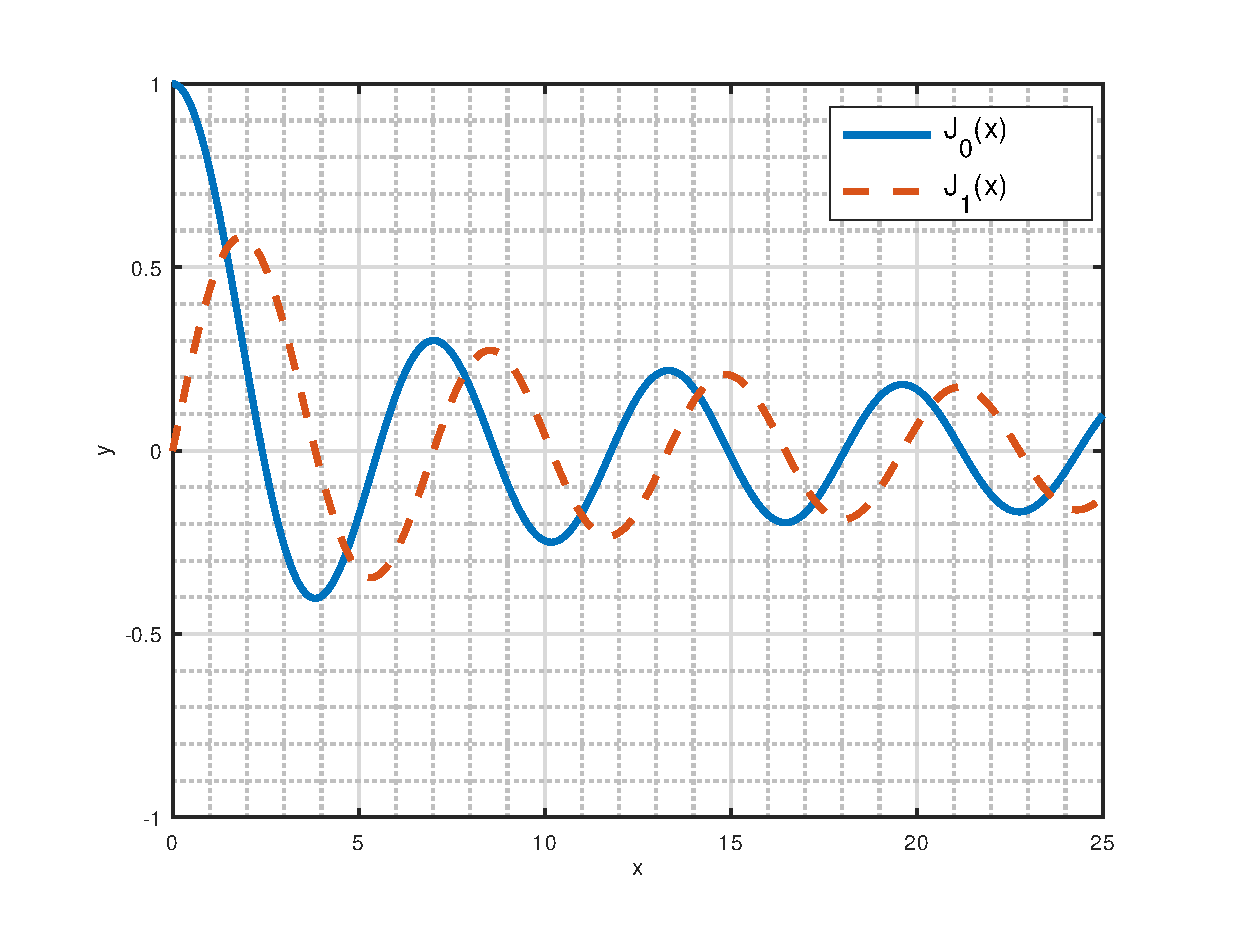
\includegraphics[scale=0.52]{bessel}\vspace{-2mm}
\caption[]{\enskip Bessel functions $J_0(x)$ and $J_1(x)$}
\label{fig:bessel}
\end{figure}
\newpage
\startexercises\label{sec9dot4}
{\small
\probs{A}
\par\noindent For Exercises 1-8 find the interval of convergence of the given
power series.
\begin{enumerate}[\bfseries 1.]
\begin{multicols}{4}
 \item $\bigsum{n = 1}{\infty}~ \dfrac{n x^n}{(n + 1)^2}$
 \item $\bigsum{n = 1}{\infty}~ \dfrac{n x^n}{2^n}$
 \item $\bigsum{n = 1}{\infty}~ n^2 \,(x - 2)^n\vphantom{\dfrac{(x + 4)^n}{2^n}}$
 \item $\bigsum{n = 0}{\infty}~ \dfrac{(x + 4)^n}{2^n}$
\end{multicols}
\begin{multicols}{4}
 \item $\bigsum{n = 1}{\infty}~ \dfrac{(x + 1)^n}{n^n}$
 \item $\bigsum{n = 1}{\infty}~ n^n \,x^n\vphantom{\dfrac{(x + 1)^n}{n^n}}$
 \item $\bigsum{n = 0}{\infty}~ (-1)^n\,x^n\vphantom{\dfrac{(x + 1)^n}{n^n}}$
 \item $\bigsum{n = 1}{\infty}~ \dfrac{n x^n}{n + 1}$
\end{multicols}
 \item Note that power series of the form $\sum_{n=0}^{\infty} a_n x^n$ have an
  issue at $x=0$ when $n=0$: $0^0$ is an indeterminate form---it can equal
  anything (or nothing). What value has it implicitly been assigned so far?
  What would be the technically correct way to write the series
  $\sum_{n=0}^{\infty} a_n x^n$ so that this issue goes away?
 \item Show that
\[
\sum_{n=1}^{\infty}\,n\,x^n ~=~ \frac{x}{(1-x)^2} \quad\text{for $~-1<x<1$.}
\]
 \item Write the following infinite series as a rational number:
\[
\frac{1}{10} \;+\; \frac{2}{100} \;+\; \frac{3}{1000} \;+\; \frac{4}{10000}
\;+\; \cdots
\]
\suspend{enumerate}
\probs{B}
\resume{enumerate}[{[\bfseries 1.]}]
 \item Differentiating term by term, verify that the Bessel function $J_0(x)$
  satisfies Bessel's equation (see equation (\ref{eqn:besseldiffeq})).
 \item Show that for all $m \ge 1$ the Bessel functions $J_m(x)$ converge for
  all $x$.
 \item For all $m \ge 1$ verify that the Bessel functions $J_m(x)$ satisfy the
  general Bessel equation of order $m$
  (see equation(\ref{eqn:besseldiffeqgen})).
 \item\label{exer:besselderiv} For the Bessel functions $J_0(x)$ and $J_1(x)$
  show that:
\begin{enumerate}[\bfseries (a)]
\item $\Ddx\,(x\,J_1(x)) ~=~ x\,J_0(x)$
\item $\int J_0(x)\,J_1(x)~\dx ~=~ -\frac{1}{2}\,J_0^2(x)$
\item $\int x\,J_0(x)\,J_1(x)~\dx ~=~ -\frac{1}{2}\,x\,J_0^2(x) ~+~
\frac{1}{2}\,\int J_0^2(x)~\dx$
\item For all integers $n\ge 2$,
\[
\int x^n\,J_0(x)~\dx ~=~ x^n\,J_1(x) ~+~ (n-1)\,x^{n-1}\,J_0(x) ~-~
(n-1)^2\,\int x^{n-2}\,J_0(x)~\dx ~.
\]
\emph{(Hint: Use part (a) and integration by parts twice.)}
\end{enumerate}
 \item For all integers $m\ge 2$ show that the Bessel functions $J_m(x)$
  satisfy the relations:
\begin{enumerate}[\bfseries (a)]
\item $m\,J_m(x) ~+~ x\,J_m'(x) ~=~ x\,J_{m-1}(x)$
\item $J_{m-1}(x) ~-~ J_{m+1}(x) ~=~ 2J_{m}'(x)$
\end{enumerate}
 \item Use long division to obtain the first three terms of
  $\frac{1}{x J_0^2(x)}$, then integrate term by term to show that
\[
J_0(x)\,\int \frac{\dx}{x J_0^2(x)} ~=~ J_0(x)\,\cdot\,\ln\,x ~+~ \frac{x^2}{4}
~-~ \frac{3x^4}{128} ~+~ \cdots ~.
\]
This function is a \emph{Bessel function of the second kind} and is another
solution of Bessel's equation.
\end{enumerate}
}
\newpage
%Begin Section 9.5
\section{Taylor's Series}
In the previous section a few functions, e.g. $f(x) = \frac{1}{1-x}$, turned out
to be the sum of a power series. This section will discuss a general method for
representing a function as a power series, called a\index{Taylor's series}
\textbf{Taylor's series}.\footnote{Named after English mathematician Brook
Taylor (1685-1731), though such series were known to others (e.g. James Gregory,
Johann Bernoulli) before Taylor.} Suppose that a function $f(x)$ can be written
as
\[
f(x) ~=~ \sum_{n=0}^{\infty}\,a_n\,(x-c)^n
\]
either for all $x$ or for $\abs{x-c} < R$, for some $R>0$. Then $f(c) = a_0$,
and differentiating term by term yields\index{Taylor's formula}
\begin{alignat*}{4}
f'(x) ~&=~ \sum_{n=1}^{\infty}\,n\,a_n\,(x-c)^{n-1} &&\Rightarrow \quad
           &f'(c) ~&=~ 1\,\cdot\,a_1\\[2pt]
f''(x) ~&=~ \sum_{n=2}^{\infty}\,n\,(n-1)\,a_n\,(x-c)^{n-2} &&\Rightarrow \quad
           &f''(c) ~&=~ 2\,\cdot\,1\,\cdot\,a_2\\[2pt]
f'''(x) ~&=~ \sum_{n=3}^{\infty}\,n\,(n-1)\,(n-2)\,a_n\,(x-c)^{n-3} &&\Rightarrow \quad
           &f'''(c) ~&=~ 3\,\cdot\,2\,\cdot\,1\,\cdot\,a_3\\
&\cdots & {} & {} & {} &\cdots\\
f^{(k)}(x) ~&=~ \sum_{n=k}^{\infty}\,n\,(n-1)\,(n-2)\,\cdots\,(n-k+1)\,a_n\,(x-c)^{n-k}
\quad &&\Rightarrow \quad &f^{(k)}(c) ~&=~ k !\;a_k
\end{alignat*}
so that in general (since $f^{(0)}(x) = f(x)$ and $0 ! = 1$):
\begin{equation}\label{eqn:taylorcoeff}
a_n ~=~ \frac{f^{(n)}(c)}{n !} \quad\text{for $~n \ge 0$}
\end{equation}
These $\seq{a_n}$ are the \textbf{Taylor's series coefficients} of $f(x)$ at
$x=c$. The full power series representation of $f(x)$ can now be stated:

\statethm{thm:taylor}{\textbf{Taylor's formula}: If $f(x)$ has a power series
representation in powers of $x-c$, where $x=c$ is inside the interval of
convergence, then that representation is unique in that interval and is given by
\begin{equation}\label{eqn:taylorseries}
f(x) ~=~ \bigsum{n=0}{\infty}~ \frac{f^{(n)}(c)}{n !}\,(x-c)^n
\end{equation}
for all $x$ in the interval. This is the \textbf{Taylor's series} for $f(x)$
about $x=c$.}
\newpage
\begin{exmp}\label{exmp:taylorexp}
\noindent Find the Taylor's series for $f(x)=e^x$ about $x=0$.\vspace{1mm}
\par\noindent\emph{Solution:} Since $\ddx\,(e^x) = e^x$, then for all $n\ge 0$,
\[
f^{(n)}(x) ~=~ e^x \quad\Rightarrow\quad f^{(n)}(0) ~=~ e^0 ~=~ 1 ~.
\]
Thus, by Taylor's formula with $c=0$:\footnote{The special case of $c=0$ in
Taylor's formula yields what is sometimes called the \emph{Maclaurin's series}
for $f(x)$,\index{Maclaurin's series} though that terminology is typically not
used in fields of study outside mathematics.}
\begin{align*}
e^x ~&=~ \bigsum{n=0}{\infty}~ \frac{f^{(n)}(0)}{n !}\,x^n ~=~
\bigsum{n=0}{\infty}~ \frac{x^n}{n !}\\
&=~ 1 ~+~ x ~+~ \frac{x^2}{2 !} ~+~ \frac{x^3}{3 !} ~+~ \frac{x^4}{4 !} ~+~
\frac{x^5}{5 !} ~+~ \cdots
\end{align*}
For what $x$ is this Taylor's series valid? Recall that Example
\ref{exmp:expseries} showed the interval of convergence is all of $\Reals$. Thus
the above Taylor's series holds for all $x$.
\end{exmp}
\divider
\vspace{2mm}

Before continuing, you might be wondering why you should even bother with
finding the Taylor's series---after all, in the above example why replace a
simple function like $e^x$ by a far more complicated expression? One reason is
that it often helps simplify some computations, especially in integrals. The
idea is to use only a few terms in the series, i.e. a polynomial, as an
approximation, since polynomials are generally easier to work with. Perhaps
surprisingly, in many practical applications no more than two terms are needed,
and often only one.

For example, using only the first two terms of the Taylor's series for
$e^x$ in Example \ref{exmp:taylorexp}, $e^x \approx 1 + x$ is a good
approximation when $x$ is close to 0 (i.e. $\abs{x} \ll 1$). Using more terms
does not necessarily help---for $\abs{x} \ll 1$ and $n>1$, $x^n$ will be
effectively 0. So the added complexity would not make the approximation
significantly better.

\begin{exmp}\label{exmp:approxe}
\noindent The energy density $E$ of electromagnetic radiation at wavelength
$\lambda$ from a black-body at temperature $T$ degrees Kelvin is given by
\emph{Planck's Law} of black-body radiation,
\[
 E(\lambda) ~=~ \frac{8\pi h c}{\lambda^5 (e^{hc/\lambda kT} - 1)}
\]
where $h$ is Planck's constant, $c$ is the speed of light, and $k$ is Boltzmann's
constant. Show that for $\lambda \gg 1$:
\[
E(\lambda) ~\approx~ \frac{8\pi kT}{\lambda^4}
\]
\par\noindent\emph{Solution:} Since $e^x ~\approx~ 1 + x\;$ for $\abs{x} \ll 1$
by the Taylor series for $e^x$, let $x = hc/\lambda kT$. Then $x \ll 1$ and so
\[
E(\lambda) ~=~ \frac{8\pi h c}{\lambda^5 (e^{hc/\lambda kT} - 1)} ~\approx~
 \frac{8\pi h c}{\lambda^5 \left(\left(1 + \frac{hc}{\lambda kT}\right) - 1\right)}
~\approx~  \frac{8\pi h c}{\lambda^5 \frac{hc}{\lambda kT}} ~\approx~
\frac{8\pi kT}{\lambda^4}
\]
\end{exmp}
\divider
\newpage
\begin{exmp}\label{exmp:taylorsin}
\noindent Find the Taylor's series for $f(x)=\sin\,x$ about $x=0$.\vspace{1mm}
\par\noindent\emph{Solution:} The derivatives of $f(x)=\sin\,x$ repeat every
four derivatives:
\[
f(x) ~=~ \sin\,x \quad,\quad
f'(x) ~=~ \cos\,x \quad,\quad
f''(x) ~=~ -\sin\,x \quad,\quad
f'''(x) ~=~ -\cos\,x \quad,\quad
f^{(4)}(x) ~=~ \sin\,x
\]
So at $x=0$:
\[
f(0) ~=~ 0 \quad,\quad
f'(x) ~=~ 1 \quad,\quad
f''(x) ~=~ 0 \quad,\quad
f'''(x) ~=~ -1 \quad,\quad
f^{(4)}(x) ~=~ 0
\]
So for $n\ge 0$,
\[
f^{(n)}(0) ~=~ \begin{cases} ~0 & \text{if $~n$ is even,}\\
~1 & \text{if $~n=1,5,9,\ldots$,}\\~-1 & \text{if $~n=3,7,11,\ldots$.}\end{cases}
\]
Thus, by Taylor's formula with $c=0$
\begin{align*}
\sin\,x ~&=~ \bigsum{n=0}{\infty}~ \frac{f^{(n)}(0)}{n !}\,x^n\\[4pt]
&=~ x ~-~ \frac{x^3}{3 !} ~+~ \frac{x^5}{5 !} ~-~ \frac{x^7}{7 !} ~+~
\frac{x^9}{9 !} ~-~ \cdots\\[4pt]
&=~ \bigsum{n=0}{\infty}~ (-1)^{n}\,\frac{x^{2n+1}}{(2n+1) !}
\end{align*}
By the Ratio Test this series converges for all $x$, since for any fixed $x$,
\[
r(x) ~=~ \lim_{n \to \infty} \;\left|\dfrac{(-1)^{n+1}\,\dfrac{x^{2n+3}}{(2n+3) !}}
{(-1)^{n}\,\dfrac{x^{2n+1}}{(2n+1) !}}\right| ~=~
x^2 \;\cdot\; \lim_{n \to \infty} \;\Biggl|\frac{1}{(2n+3)\,(2n+2)}\Biggr| ~=~ 0 ~<~ 1 ~.
\]
\end{exmp}
\begin{exmp}\label{exmp:taylorcos}
\noindent Find the Taylor's series for $f(x)=\cos\,x$ about $x=0$.\vspace{1mm}
\par\noindent\emph{Solution:} The Taylor's series can be found using the same
procedure as in Example \ref{exmp:taylorsin}, but it is simpler to just
differentiate the Taylor's series for $\sin\,x$ term by term for all $x$:
\begin{align*}
\cos\,x ~&=~ \ddx\,(\sin\,x) ~=~
\ddx\,\left(x ~-~ \frac{x^3}{3 !} ~+~ \frac{x^5}{5 !} ~-~ \frac{x^7}{7 !} ~+~
\frac{x^9}{9 !} ~-~ \cdots\right)\\[4pt]
&=~ 1 ~-~ \frac{x^2}{2 !} ~+~ \frac{x^4}{4 !} ~-~ \frac{x^6}{6 !} ~+~
\frac{x^8}{8 !} ~-~ \cdots\\[4pt]
&=~ \bigsum{n=0}{\infty}~ (-1)^{n}\,\frac{x^{2n}}{(2n) !}
\end{align*}
Since the Taylor's series for $\sin\,x$ converges for all $x$ then so does its
derivative. Thus the Taylor's series for $\cos\,x$ converges for all
$x$.\\Notice that the Taylor's series for $\cos\,x$ has only even powers of $x$, while
the series for $\sin\,x$ has only odd powers of $x$. This makes sense since
$\cos\,x$ and $\sin\,x$ are even and odd functions, respectively.
\end{exmp}
\divider
\newpage
\begin{exmp}\label{exmp:taylorlog}
\noindent The function $\ln\,x$ is not defined at $x=0$ and hence has no
Taylor's series about $x=0$. Instead, find the Taylor's series for
$f(x)=\ln\,(1+x)$ about $x=0$.\vspace{1mm}
\par\noindent\emph{Solution:} Take successive derivatives:
\[
f(x) ~=~ \ln\,(1+x) \quad,\quad
f'(x) ~=~ \frac{1}{1+x} \quad,\quad
f''(x) ~=~ -\frac{1}{(1+x)^2} \quad,\quad
f'''(x) ~=~ \frac{1 \,\cdot\, 2}{(1+x)^3} \quad,\quad
f^{(4)}(x) ~=~ -\frac{1 \,\cdot\, 2 \,\cdot\, 3}{(1+x)^4}
\]
So $f(0)=0$ and for $n\ge 1$:
\[
f^{(n)}(x) ~=~ (-1)^{n-1}\,\frac{(n-1) !}{(1+x)^n} \quad\Rightarrow\quad
f^{(n)}(0) ~=~ (-1)^{n-1}\,(n-1) !
\]
Thus, by Taylor's formula,
\begin{align*}
\ln\,(1+x) ~&=~ \bigsum{n=0}{\infty}~ \frac{f^{(n)}(0)}{n !}\,x^n ~=~
\bigsum{n=1}{\infty}~ (-1)^{n-1}\,\frac{(n-1) !\,x^{n}}{n !}\\[4pt]
&=~ \bigsum{n=1}{\infty}~ (-1)^{n-1}\,\frac{x^{n}}{n}\\[4pt]
&=~ x ~-~ \frac{x^2}{2} ~+~ \frac{x^3}{3} ~-~ \frac{x^4}{4} ~+~
\frac{x^5}{5} ~-~ \cdots
\end{align*}
Use the Ratio Test to find the interval of convergence:
\[
r(x) ~=~ \lim_{n \to \infty} \;\left|\dfrac{(-1)^{n}\,\dfrac{x^{n+1}}{n+1}}
{(-1)^{n-1}\,\dfrac{x^{n}}{n}}\right| ~=~
\abs{x} \;\cdot\; \lim_{n \to \infty} \;\Biggl|\frac{n}{n+1}\Biggr| ~=~
\abs{x} \,\cdot\, 1 ~=~ \abs{x}
\]
So the series converges when $\abs{x} < 1$. Check the cases $r(x)=\abs{x}=1$
individually. For $x=1$ the series is the alternating harmonic series
$\sum_{n=1} \frac{(-1)^{n-1}}{n}$, which converges. For $x=-1$ the series is
$-\sum_{n=1} \frac{1}{n}$, the negative of the harmonic series, which diverges.
Thus, the series converges for $-1<x\le 1$.
\end{exmp}
\begin{exmp}\label{exmp:taylorexp2}
\noindent Find the Taylor's series for $f(x)=e^{x^2}$ about $x=0$.\vspace{1mm}
\par\noindent\emph{Solution:} The Taylor's series can be found using the same
procedure as in Example \ref{exmp:taylorexp}, but it is simpler to just
replace each occurrence of $x$ in the Taylor's series for $e^x$ by $x^2$ (since
the series for $e^x$ converges for all $x$). In
other words, make the substitution $u=x^2$ in the Taylor's series for $e^u$
about $u=0$:
\begin{align*}
e^u ~&=~ \bigsum{n=0}{\infty}~ \frac{u^n}{n !}\\[4pt]
e^{x^2} ~&=~ \bigsum{n=0}{\infty}~ \frac{(x^2)^n}{n !} ~=~
\bigsum{n=0}{\infty}~ \frac{x^{2n}}{n !}\\[4pt]
&=~ 1 ~+~ x^2 ~+~ \frac{x^4}{2 !} ~+~ \frac{x^6}{3 !} ~+~
\frac{x^8}{4 !} ~+~ \frac{x^{10}}{5 !} ~+~ \cdots
\end{align*}
\end{exmp}
\divider
\newpage
\noindent Define the \textbf{$\bm{n}$-th degree Taylor polynomial} $P_n(x)$ for
a function $f(x)$ about $x=c$ by\index{Taylor polynomial}
\begin{align*}
P_n(x) ~&=~ \bigsum{k=0}{n}~ \frac{f^{(k)}(c)}{k !}\,(x-c)^k\\
&=~ f(c) ~+~ \frac{f'(c)}{1 !}\,(x-c) ~+~ \frac{f''(c)}{2 !}\,(x-c)^2 ~+~ \cdots ~+~
\frac{f^{(n)}(c)}{n !}\,(x-c)^n
\end{align*}
for $x$ in the interval of convergence for the full Taylor's series. In other
words, $P_n(x)$ is the $n$-th partial sum of the Taylor's series. Since some of
the coefficients could be zero, $P_n(x)$ is a polynomial of degree at most
$n$. Thus, $P_n(x) = O(x^n)$. For that reason $P_n(x)$ is
sometimes called the \textbf{$\bm{O(x^n)}$ approximation} to $f(x)$.

Figure \ref{fig:sinetaylor} shows a comparison of $\sin\,x$ with a few
of its approximations:\vspace{-3mm}

\begin{figure}[ht]
\centering
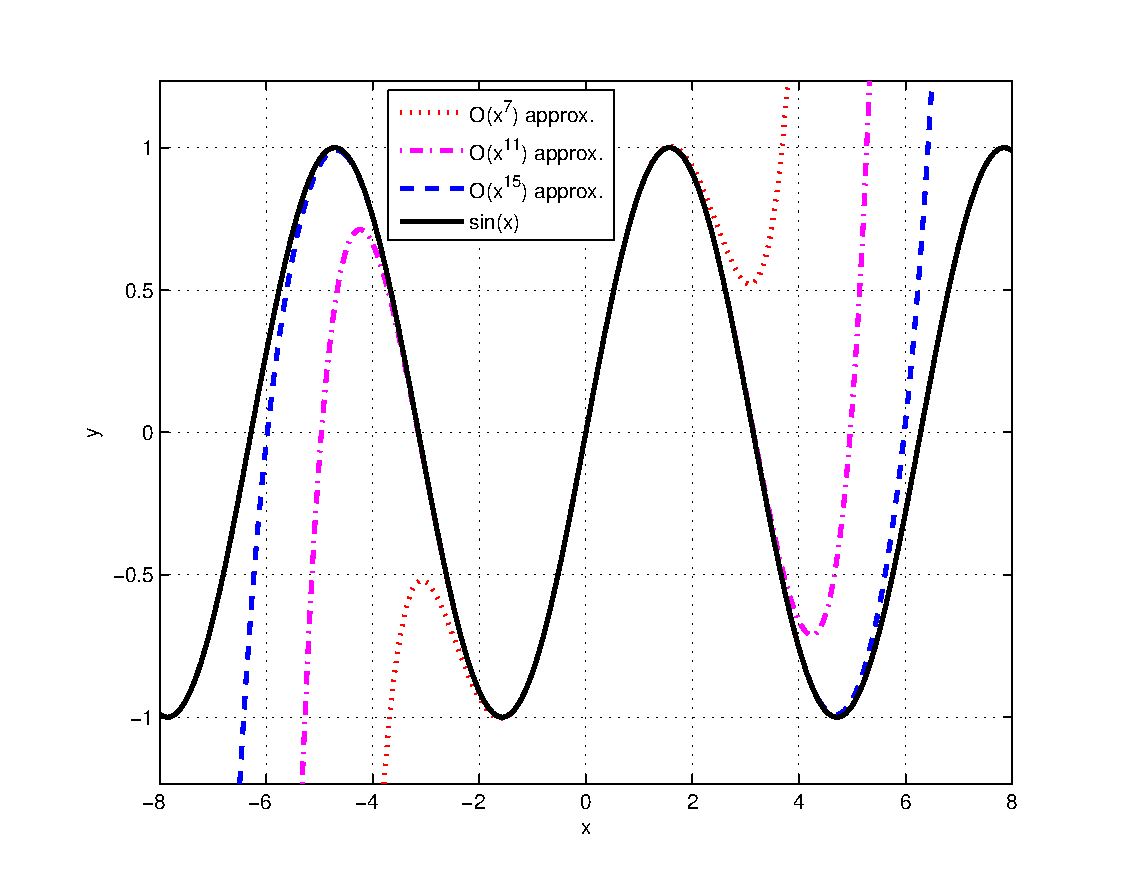
\includegraphics[scale=0.70]{sinetaylor}\vspace{-2mm}
\caption[]{\enskip $\sin\,x$ and Taylor's series approximations}
\label{fig:sinetaylor}
\end{figure}

As you can see, the Taylor polynomials of degree 7, 11 and 15 are all good
approximations over the interval $\ival{-2}{2}$, with the $O(x^{15})$
approximation still being fairly good over $\ival{-6}{6}$. Clearly those
approximations all become poor quite quickly for $\abs{x} > 6$; they approach
$\pm\infty$, unlike $\sin\,x$.

The following theorem shows how to measure the accuracy of the
approximations:
\newpage
\statethm{thm:taylorremainder}{\textbf{Remainder Theorem}:\footnotemark If
$P_n(x)$ is the $n$-th degree Taylor polynomial about $x=c$ for a function
$f(x)$ in some interval containing $x=c$, then for all $x$ in that interval,
\begin{equation}\label{eqn:taylorremainder}
f(x) ~=~ P_n(x) ~+~ R_n(x) ~,
\end{equation}
where
\begin{equation}\label{eqn:taylorrem1}
R_n(x) ~=~ \frac{f^{(n+1)}(c +\theta (x-c))}{(n+1) !}\,(x-c)^{n+1}
\end{equation}
for some number $\theta$ between 0 and 1. Alternatively,
\begin{equation}\label{eqn:taylorrem2}
R_n(x) ~=~ \frac{1}{n !}\,\int_c^x (x-t)^{n}\,f^{(n+1)}(t)~\dt ~.
\end{equation}
}\footnotetext{For a proof see
pp.171-172 in \textsc{Klambauer, G.}, \emph{Aspects of Calculus}, New York:
Springer-Verlag, 1986.}\index{Taylor's series!Remainder Theorem}

Since the number $\theta$ is unknown in equation (\ref{eqn:taylorrem1}),
usually only an upper bound on the remainder $R_n(x)$ can be found by that
formula. For practical purposes formula (\ref{eqn:taylorrem2}) for $R_n(x)$
might be easier to use (via numerical integration).

A common misconception is that hand-held calculators use Taylor's series to
compute values of functions like $\sin\,x$, $\cos\,x$, $e^x$, etc. However, that
is typically well beyond their capability, especially for large values of
$x$---far too
many terms would be required. Instead, many calculators use an algorithm called
CORDIC\footnote{See Ch.7 in \textsc{Schmid, H.}, \emph{Decimal Computation},
New York: John Wiley \& Sons, Inc., 1974.}
(Coordinate Rotation Digital Computer), and---perhaps\index{CORDIC}
surprisingly---lookup tables. CORDIC uses the computationally
inexpensive operation of bit-shifting to translate large input values into a
smaller range, then uses tables stored in memory for values in that range, along
with interpolation for numbers between those in the tables.\footnote{To see how
inaccurate calculators can be, compute $\tan (355/226)$ in radian mode on a
calculator. The true value to 3 decimal places is $-7497258.185$, but few
calculators produce an answer close to that.}

\divider
\vspace{2mm}
\startexercises\label{sec9dot5}
{\small
\probs{A}
\par\noindent For Exercises 1-9 write out the first three nonzero terms in the
Taylor's series for the given function $f(x)$ about the given value $c$. You may
use any method you like.
\begin{enumerate}[\bfseries 1.]
\begin{multicols}{3}
 \item $f(x) = \sin\,x$ ; $c = \pi/2$
 \item $f(x) = \sinh\,x$ ; $c = 0$
 \item $f(x) = \cosh\,x$ ; $c = 0$
\end{multicols}
\begin{multicols}{3}
 \item\label{exer:taylortan} $f(x) = \tan\,x$ ; $c = 0$
 \item\label{exer:taylortanh} $f(x) = \tanh\,x$ ; $c = 0$
 \item $f(x) = \sec\,x$ ; $c = 0$
\end{multicols}
\begin{multicols}{3}
 \item\label{exer:tayloratan} $f(x) = \dfrac{1}{1 +x^2}$ ; $c = 0$
 \item $f(x) = \dfrac{1}{1 + x^2}$ ; $c = 1$
 \item\label{exer:taylorsq} $f(x) = \sqrt{1 + x^2}$ ; $c = 0\vphantom{\dfrac{1}{x^2 ~+~ 1}}$
\end{multicols}
 \item Use Example \ref{exmp:seriesderivxn} from Section 9.4 to write out the
  first three nonzero terms in the Taylor's series for
  $f(x) = \frac{1}{(1 - x)^3}$ about $x=0$.
 \item Use the derivative of the Taylor's series for $\sqrt{1 + x^2}$ from
  Exercise \ref{exer:taylorsq} to write out the first three nonzero terms in the
  Taylor's series for $f(x) ~=~ \frac{x^2}{\sqrt{1 + x^2}}$ about $x=0$.
\suspend{enumerate}
\par\noindent For Exercises 12-15 replace the function $f(x)$ by its Taylor's
 series about $x=0$ to evaluate the given indefinite integral $\int f(x) \;\dx$
 (up to the first three nonzero terms in the series).
\resume{enumerate}[{[\bfseries 1.]}]
\begin{multicols}{4}
 \item $\displaystyle\int \frac{\sin\,x}{x}~\dx$
 \item $\displaystyle\int \cos\,(x^2)~\dx\vphantom{\displaystyle\int \frac{\sin\,x}{x}}$
 \item $\displaystyle\int e^{-x^2}~\dx\vphantom{\displaystyle\int \frac{\sin\,x}{x}}$
 \item $\displaystyle\int \sqrt{1+x^6}~\dx\vphantom{\displaystyle\int \frac{\sin\,x}{x}}$
\end{multicols}
 \item\label{exer:atanpi} Use $\ddx\,(\tan^{-1} x) = \frac{1}{1+x^2}$ along with
  Exercise \ref{exer:tayloratan} to find the Taylor's series for
  $f(x)=\tan^{-1} x$ about $x=0$, along with its interval of convergence.
 \item Use Exercise \ref{exer:atanpi} to show that
\[
\pi ~=~ 4\,\left(1 \;-\; \frac{1}{3} \;+\; \frac{1}{5} \;-\; \frac{1}{7}
\;+\; \cdots \right) ~.
\]
 \item Use the first three nonzero terms in the Taylor's series about $x=0$ for
 $e^{-x^2/2}$ to evaluate the definite integral
 \begin{displaymath}
  \int_{-1}^1 ~\frac{1}{\sqrt{2\pi}} \,e^{-x^2/2}~\dx \quad .
 \end{displaymath}
  Note: The actual value (rounded to 4 decimal places) is 0.6826.
 \item Recall that the surface area $S$ of the solid obtained by revolving the
  curve $y = x^2$ around the $x$-axis between $x = 0$ and $x = 2$ is given by
  the integral
 \begin{displaymath}
  S ~=~ \int_0^2 ~2 \pi x^2 \,\sqrt{1 \;+\; 4x^2}~\dx \quad .
 \end{displaymath}
 The exact value of the integral rounded to 3 decimal places is $S = 53.226$.
 Use the first two nonzero terms in the Taylor's series for $\sqrt{1 + 4x^2}$
 about $x=0$ to approximate the integral. How close is this approximation to the
 actual value? Does the approximation become better if you use the first three
 nonzero terms in the Taylor's series? Justify your answer.
 \item The tangential component of a space shuttle's velocity during reentry is
 approximately
\[
 v(t) ~=~ v_c \,\tanh\,\left( \frac{g}{v_c} t ~+~
 \tanh^{-1} \left(\frac{v_0}{v_c}\right) \right)
\]
  where $v_0$ is the velocity at time $t=0$ and $v_c$ is the terminal velocity.
  If $\tanh^{-1} \left(\frac{v_0}{v_c}\right) = \frac{1}{2}$ then show that
  $v(t) \approx gt + \frac{1}{2}v_c$.
 \item The velocity of a water wave of length $L$ in water of depth $h$
 satisfies the equation
 $v^2 = \frac{gL}{2\pi} \tanh \left( \frac{2\pi h}{L}\right)$. Show that
 $v \approx \sqrt{gh}$.
 \item A disk of radius $a$ has a charge of constant density $\sigma$. A point
 $P$ lies at a distance $r$ directly above the disk. The
 \emph{electrical potential} $V$ at point $P$ is given by
 $V = 2\pi\sigma(\sqrt{r^2 + a^2} - r)$. Show that
 $V \approx \frac{\pi a^2 \sigma}{r}$ for large $r$ (i.e. $r \gg 1$).
 \item The fifth-degree \emph{Pad\'{e} approximation} uses rational functions to
  approximate $\tanh\,x$:\index{Pad\'{e} approximation}
\[
 \tanh\,x ~\approx~ \frac{x^5 + 105x^3 + 945x}{15x^4 + 420x^2 + 945}
\]
 Compare the values of the Pad\'{e} approximation and the fifth-degree Taylor's
 series approximation from Exercise \ref{exer:taylortanh}, evaluated at $x=1$.
 Which is better? The actual value of $\tanh (1)$ is 0.7615941559558. How do
 the two approximations compare at $x=2$?
\end{enumerate}
}

\newpage
%Put the bibliography here
\fancyhf{}
\fancyhf{}
\fancyhead[LE]{\tikzstyle{headbox} = [fill=headercolor,line width=0pt,rectangle,
 rounded corners]
 \begin{tikzpicture}
  \node [headbox] (box){%
   \begin{minipage}{\fminilength}%
     \sffamily{\bfseries\thepage\qquad \enskip\leftmark}
    \end{minipage}%
  };
 \end{tikzpicture}}
\fancyhead[LO]{\tikzstyle{headbox} = [fill=headercolor,line width=0pt,rectangle,
 rounded corners]
 \begin{tikzpicture}
  \node [headbox] (box){%
   \begin{minipage}{\fminilength}%
     \sffamily {}\hfill{\bfseries{\leftmark\qquad\thepage}}
    \end{minipage}%
  };
 \end{tikzpicture}}
%\titleformat{\chapter}[display]
%  {\filcenter\huge\selectfont\bfseries\sffamily}
%  {}{0mm}{\titlerule[1.5pt]\vspace{3mm}}[\vspace{3mm}{\titlerule[1.5pt]}]
%\include{calc12book-biblio}
%Put appendices here
\titleformat{\chapter}[display]
  {\filcenter\LARGE\selectfont\bfseries\sffamily}
  {\titlerule[1.5pt]\vspace{3mm}\MakeUppercase{\chaptertitlename}
   \thechapter}{3mm}
  {\titlerule[1.5pt]\vspace{3mm}\huge}
\titleformat*{\section}{\Large\bfseries\sffamily}
\fancyhf{}
\fancyhead[LE]{\tikzstyle{headbox} = [fill=headercolor,line width=0pt,rectangle,rounded corners]
 \begin{tikzpicture}
  \node [headbox] (box){%
   \begin{minipage}{\fminilength}%
     \sffamily{\bfseries\thepage\qquad \enskip Appendix A:\quad\leftmark}
    \end{minipage}%
  };
 \end{tikzpicture}}
\fancyhead[LO]{\tikzstyle{headbox} = [fill=headercolor,line width=0pt,rectangle,rounded corners]
 \begin{tikzpicture}
  \node [headbox] (box){%
   \begin{minipage}{\fminilength}%
     \sffamily {}\hfill{\bfseries{Appendix A:\quad\leftmark\qquad\thepage}}
    \end{minipage}%
  };
 \end{tikzpicture}}
\begin{appendices}
 \chapter{Answers and Hints to Selected Exercises}
\begin{multicols*}{2}
\section*{Chapter 1}
\subsection*{Section 1.1 (p. \pageref{sec1dot1})}
\textbf{1.} $2t$ \quad
\textbf{2.} $19.6t$ \quad
\textbf{3.} $-32t+2$ \quad
\textbf{4.} $3t^2$
\subsection*{Section 1.2 (p. \pageref{sec1dot2})}
\textbf{1.} $0$ \quad \textbf{3.} $2x+2$ \quad
\textbf{5.} $-\frac{1}{(x+1)^2}$ \quad
\textbf{7.} $-\frac{2}{x^3}$\\
\textbf{9.} $\frac{1}{2\sqrt{x+1}}$ \quad
\textbf{11.} $\frac{2x+3}{2\sqrt{x^2+3x+4}}$
\subsection*{Section 1.3 (p. \pageref{sec1dot3})}
\textbf{5.} Hint: Use the sine double-angle formula. \quad
\textbf{7.} Hint: Use
Exercise 5 and the sine addition formula.
\subsection*{Section 1.4 (p. \pageref{sec1dot4})}
\textbf{1.} $2x-1$ \quad \textbf{3.} $4x^5 + \frac{9}{x^7}$ \quad
\textbf{5.} $x\,\cos x + \sin x$\\
\textbf{7.} $\frac{x\,\cos x - \sin x}{x^2}$
\quad \textbf{9.} $\frac{2-2t^2}{(1+t^2)^2}$ \quad
\textbf{11.} $\frac{ad-bc}{(cx+d)^2}$\\
\textbf{13.} $2\pi r$
\subsection*{Section 1.5 (p. \pageref{sec1dot5})}
\textbf{1.} $-20(1-5x)^3$ \quad \textbf{3.} $-\frac{1}{\sqrt{1-2x}}$ \quad
\textbf{5.} $\frac{1-x}{2\sqrt{x}(x+1)^2}$\\
\textbf{7.} $-\frac{8(1-t)^3}{(1+t)^5}$
\textbf{9.} $2\sin x \,\cos x$ \quad
\textbf{11.} $15\sec^2(5x)$\\
\textbf{13.} $2x\sec (x^2)\,\tan (x^2)$ \quad
\textbf{15.} $\beta (1-\beta^2)^{-3/2}$\\
\textbf{17.} $\sin (\cos x)\,\sin x$ \quad
\textbf{21.} Hint for part(b): Use part(a) and the
Chain Rule to find $S_p$, then recall how to convert from radians per second to
revolutions per minute.
\subsection*{Section 1.6 (p. \pageref{sec1dot6})}
\textbf{1.} $6x+2$ \quad
\textbf{3.} $-9\cos 3x$ \quad
\textbf{5.} $\frac{2}{x^3}$
\section*{Chapter 2}
\subsection*{Section 2.1 (p. \pageref{sec2dot1})}
\textbf{1.} $f^{-1}(x)=x$, $\left(f^{-1}\right)'(x)=1$\\
\textbf{3.} $f^{-1}(x)=\sqrt{x}$, $\left(f^{-1}\right)'(x)=\frac{1}{2\sqrt{x}}$\\
\textbf{5.} $f^{-1}(x)=\frac{1}{x}$, $\left(f^{-1}\right)'(x)=-\frac{1}{x^2}$\\
\textbf{7.} $f^{-1}(x)=\frac{1}{\sqrt{x}}$, $\left(f^{-1}\right)'(x)=-\frac{1}{2}x^{-3/2}$
\subsection*{Section 2.2 (p. \pageref{sec2dot2})}
\textbf{1.} $6\sec^2 3x\,\tan 3x$ \quad
\textbf{3.} $-3\csc^2 3x$ \quad
\textbf{5.} $\frac{3}{9+x^2}$\\
\textbf{7.} $-\frac{3}{1+9x^2}$ \quad
\textbf{9.} $\frac{1}{1+x^2}$ \quad
\textbf{11.} $\frac{6\sin^{-1} 3x}{\sqrt{1-9x^2}}$\\
\textbf{13.} $\frac{1}{1+x^2}$ \quad
\textbf{15.} $\cot^{-1} x - \frac{x}{1+x^2}$
\subsection*{Section 2.3 (p. \pageref{sec2dot3})}
\textbf{1.} $2e^{2x}$ \quad
\textbf{3.} $-e^{-x} - e^x$ \quad
\textbf{5.} $\frac{2e^x}{(1-e^x)^2}$ \quad
\textbf{7.} $e^{e^x}e^x$\\
\textbf{9.} $\frac{1}{x}$ \quad
\textbf{11.} $\frac{6x\left(\ln\left(\tan x^2\right)\right)^2 \sec^2 x^2}{\tan x^2}$\\
\textbf{15.} $x^{x^2}(x+2x\ln x)$\\
\textbf{17.} $x^{\sin x}\left(\cos x \, \ln x + \frac{\sin x}{x}\right)$ \quad
\textbf{19.} $15.5$ hours\\
\textbf{21.} $12$ hours
\subsection*{Section 2.4 (p. \pageref{sec2dot4})}
\textbf{1.} $\frac{\ln 3\,\left(3^x - 3^{-x}\right)}{2}$ \quad
\textbf{3.} $(\ln 2)^2 \, 2^{2^x} \, 2^x$\\
\textbf{5.} $\frac{2x}{(\ln 2)(x^2+1)}$ \quad
\textbf{7.} $\frac{\cos\left(\log_2 \pi x\right)}{x \ln 2}$ \quad
\textbf{9.} $3x^2$
\section*{Chapter 3}
\subsection*{Section 3.1 (p. \pageref{sec3dot1})}
\textbf{1.} $y=4x-3$ \quad
\textbf{3.} $y=-6x+10$ \quad
\textbf{5.} $y=4x$\\
\textbf{7.} $y=x+3$ \quad
\textbf{9.} $y=240x+176$ \quad
\textbf{11.} $y=2x$\\
\textbf{13.} $y=3x + \frac{31}{27}$, $y=3x+1$ \quad
\textbf{15.} $75.96\Degrees$\\
\textbf{17.} $0\Degrees$ \quad
\textbf{19.} $116.6\Degrees$ \quad
\textbf{21.} $5.71\Degrees$\\
\textbf{23.} $y=-\tfrac{1}{4}x+\tfrac{11}{2}$\\
\textbf{25.} $y=-\frac{1}{4}x-\tfrac{81}{4}$, $y=-\frac{1}{4}x+\tfrac{1159}{108}$
\subsection*{Section 3.2 (p. \pageref{sec3dot2})}
\textbf{1.} $\frac{7}{3}$ \quad
\textbf{3.} $0$ \quad
\textbf{5.} $-1$ \quad
\textbf{7.} $0$ \quad
\textbf{9.} $2$ \quad
\textbf{11.} $0$\\
\textbf{14.} $\frac{1}{2}$ \quad
\textbf{15.} $0$ \quad
\textbf{17.} $0$
\subsection*{Section 3.3 (p. \pageref{sec3dot3})}
\textbf{1.} continuous \quad
\textbf{3.} discontinuous\\
\textbf{5.} discontinuous \quad
\textbf{7.} discontinuous\\
\textbf{9.} continuous \quad
\textbf{11.} continuous\\
\textbf{13.} continuous \quad
\textbf{15.} discontinuous\\
\textbf{17.} continuous \quad
\textbf{19.} $1$ \quad
\textbf{21.} $e^{-1}$\\
\textbf{25.} Hint: Use the Intermediate Value Theorem.
\subsection*{Section 3.4 (p. \pageref{sec3dot4})}
\textbf{1.} $\frac{-3x^2y + 4y^2 + 2x}{x^3 - 8xy - 1}$ \quad
\textbf{3.} $\frac{2(x-y+1) - 3(x+y)^2}{2(x-y+1) + 3(x+y)^2}$\\
\textbf{5.} $\frac{2x(1 - (x^2 - y^2))}{y(2(y^2 - x^2) - 1)}$ \quad
\textbf{7.} $-\frac{y}{x}$\\
\textbf{9.} $-\frac{-2x - y + 3x^2y^2e^{\sin (xy)} + x^3y^3e^{\sin (xy)}\cos (xy)}{x^4y^2e^{\sin (xy)}\cos (xy)
+ 2x^3ye^{\sin (xy)} - 3y^2 - x}$\\
\textbf{13.} $-\frac{x^2 + y^2}{y^3}$
\subsection*{Section 3.5 (p. \pageref{sec3dot5})}
\textbf{1.} $80\pi$ ft/s \quad
\textbf{3.} $2.4$ ft/s \quad
\textbf{5.} $10$ ft/s\\
\textbf{7.} $-76\pi$ cm\textsuperscript{3}/min \quad
\textbf{9.} $45.14$ mph\\
\textbf{11.} $155.8$ ft/min
\subsection*{Section 3.6 (p. \pageref{sec3dot6})}
\textbf{1.} $(2x-2)\,\dx$ \quad
\textbf{2.} $4x\,\sin (x^2)\,\cos (x^2)\,\dx$\\
\textbf{11.} Hint: Mimic Example \ref{exmp:diff4}.
\section*{Chapter 4}
\subsection*{Section 4.1 (p. \pageref{sec4dot1})}
\textbf{1.} $(1,1)$ \quad
\textbf{3.} $125,000$ sq yd \quad
\textbf{5.} $U = \frac{V}{2}$\\
\textbf{7.} $R=r$ \quad
\textbf{9.} $2ab$ \quad
\textbf{13.} $Q=\sqrt{\frac{2DP}{I+W}}$\\
\textbf{15.} $r=\sqrt{r_0^2 + x_0^2}$ \quad
\textbf{17.} $380.62$ minutes\\
\textbf{19.} $12\pi \sqrt{3}$ \quad
\textbf{21.} $12.8$ ft \quad
\textbf{22.} Hint: Place the right angle of the triangle at the origin in the $xy$-plane. \quad
\textbf{25.} $x = \sqrt{\frac{RN}{r}}$\\
\textbf{27.} $x=\frac{a}{\sqrt{2}}$ \quad
\textbf{33.} $(a^{2/3} + b^{2/3})^{3/2}$\\
\textbf{34.} Hint: You can leave your answer in terms of $R$ and an angle satisfying
a certain equation.
\subsection*{Section 4.2 (p. \pageref{sec4dot2})}
\textbf{2.} local maximum at $x=0$, local minimum at $x=2$, inflection pt at $x=1$,
increasing for $x<0$ and $x>2$, decreasing for $0<x<2$, concave up for $x>1$,
concave down for $x<1$\\
\textbf{3.} local maximum at $x=1$, inflection pt at $x=2$, increasing for $x<1$,
decreasing for $x>1$, concave up for $x>2$, concave down for $x<2$, horizontal
asymptote: $y=0$\\
\textbf{5.} local maximum at $x=0$, inflection pts at $x=\pm \frac{1}{\sqrt{3}}$,
increasing for $x<0$, decreasing for $x>0$, concave up for $x<-\frac{1}{\sqrt{3}}$ and
$x>\frac{1}{\sqrt{3}}$, concave down for $-\frac{1}{\sqrt{3}}<x<\frac{1}{\sqrt{3}}$,
horizontal asymptote: $y=0$\\
\textbf{7.}  local maximum at $x=\ln 2$, inflection pt at $x=\ln 4$,
increasing for $x<\ln 2$, decreasing for $x>\ln 2$, concave up for $x>\ln 4$,
concave down for $x<\ln 4$, horizontal asymptote: $y=0$
\subsection*{Section 4.3 (p. \pageref{sec4dot3})}
\textbf{1.} $x=0.450184$ \quad
\textbf{3.} $x=0.567143$\\
\textbf{5.} $x=1.414213$ \quad
\textbf{11.} global maximum at $x=2.8214$ \quad
\textbf{14.} $50$
\subsection*{Section 4.4 (p. \pageref{sec4dot4})}
\textbf{1.} No \quad
\textbf{3.} Yes \quad
\textbf{6.} No \quad
\textbf{18.} Hint: Calculate $f'(x)$ and use the cosine addition formula.
\section*{Chapter 5}
\subsection*{Section 5.1 (p. \pageref{sec5dot1})}
\textbf{1.} $\frac{x^3}{3} + \frac{5x^2}{2} - 3x + C$ \quad
\textbf{3.} $4e^x + C$\\
\textbf{5.} $-5 \cos x + C$ \quad
\textbf{7.} $6 \ln \abs{x} + C$\\
\textbf{9.} $-\frac{4}{3}x^{3/2} + C$ \quad
\textbf{11.} $\frac{x^2}{2} + \frac{3}{7}x^{7/3} + C$\\
\textbf{13.} $3 \sec x + C$ \quad
\textbf{15.} $-7 \cot x + C$
\subsection*{Section 5.2 (p. \pageref{sec5dot2})}
\textbf{3.} $\frac{1}{2}$ \quad
\textbf{4.} $\frac{1}{3}$ \quad
\textbf{5.} $1$ \quad
\textbf{6.} $\frac{1}{4}$
\subsection*{Section 5.3 (p. \pageref{sec5dot3})}
\textbf{1.} $\frac{1}{3}$ \quad
\textbf{3.} $\frac{1}{4}$ \quad
\textbf{5.} $\frac{1}{2}$ \quad
\textbf{7.} $1$ \quad
\textbf{9.} $2e - 2e^{-1}$\\
\textbf{11.} $\frac{16}{3}$
\subsection*{Section 5.4 (p. \pageref{sec5dot4})}
\textbf{1.} $\frac{3 \sin 5x \,-\, 4 \cos 5x}{5} + C$\\
\textbf{3.} $-\frac{1}{2} e^{-x^2} + \frac{1}{3} \sin x^3 ~+~ C$\\
\textbf{5.} $\ln (1 + e^x) + C$\\
\textbf{7.} $\frac{2}{5} (x+4)^{5/2} - \frac{8}{3} (x+4)^{3/2} + C$\\
\textbf{9.} $\tan x - x + C$ \quad
\textbf{11.} $\frac{3}{10} \tan^{-1} \left(\frac{5x}{2}\right) + C$\\
\textbf{13.} $10$ \quad
\textbf{15.} $\frac{1192}{15}$ \quad
\textbf{17.} $1$ \quad
\textbf{19.} $-\frac{1}{48}$\\
\textbf{21.} $\frac{\pi}{6}$ \quad
\textbf{23.} $\frac{1}{2}$
\subsection*{Section 5.5 (p. \pageref{sec5dot5})}
\textbf{1.} $\frac{1}{2}$ \quad
\textbf{3.} $1$ \quad
\textbf{5.} divergent \quad
\textbf{7.} $\frac{1}{\ln 2}$\\
\textbf{9.} divergent \quad
\textbf{11.} $6$ \quad
\textbf{13.} divergent\\
\textbf{15.} $\frac{\pi}{2}$ \quad
\textbf{19.} Yes \quad
\textbf{20.} No
\section*{Chapter 6}
\subsection*{Section 6.1 (p. \pageref{sec6dot1})}
\textbf{1.} $\frac{x^2 \ln x}{2} - \frac{x^2}{4} + C$ \quad
\textbf{2.} $(x^2 - 2x + 2)e^x + C$\\
\textbf{3.} $x \sin x + \cos x + C$\\
\textbf{5.} $\frac{x^2 a^x}{\ln a} - \frac{2x a^x}{\ln^2 a} + \frac{2 a^x}{\ln^3 a} + C$\\
\textbf{7.} $x \ln x^2 - 2x + C$\\
\textbf{9.} Hint: Use a double-angle identity.\\
\textbf{11.} $x \sin^{-1} x + \sqrt{1-x^2} + C$\\
\textbf{13.} $x \tan^{-1} 3x - \frac{1}{6}\ln (1+9x^2) + C$\\
\textbf{15.} $-\frac{3}{8}\sin x \cos 3x + \frac{1}{8}\cos x \sin 3x + C$\\
\textbf{17.} $\frac{1}{4}x^4 \ln^2 x - \frac{1}{8}x^4 \ln x + \frac{1}{32}x^4 + C$ \quad
\textbf{19.} $\frac{16}{3}$\\
\textbf{20.} $\frac{2\sqrt{2}+2}{15}$ \quad
\textbf{21.} $\frac{x \sin (\ln x)}{2} - \frac{x \cos (\ln x)}{2} + C$\\
\textbf{23.} $\frac{x^2 \tan^{-1} x}{2} - \frac{x}{2} + \frac{\tan^{-1} x}{2} + C$\\
\textbf{24.} $x \cot^{-1} \sqrt{x} + \sqrt{x} + \cot^{-1} \sqrt{x} + C$\\
\textbf{25.} Hint: Try the substitution $t=\sqrt{x}$.
\subsection*{Section 6.2 (p. \pageref{sec6dot2})}
\textbf{1.} $-\frac{1}{14}\cos\,7x + \frac{1}{6}\cos\,3x + C$\\
\textbf{3.} $-\frac{1}{14}\sin\,7x + \frac{1}{6}\sin\,3x + C$\\
\textbf{5.} $-\frac{2}{5}\cos^{5/2}x + \frac{2}{9}\cos^{9/2}x + C$\\
\textbf{7.} $-\frac{1}{4}\sin\,2x + \frac{1}{48}\sin^2 2x + \frac{5}{16}x + \frac{3}{64}\sin\,4x+ C$\\
\textbf{9.} $\frac{1}{3}\tan^3 x + \tan\,x + C$ \quad
\textbf{11.} $\frac{1}{4}\sin^4 x + C$
\subsection*{Section 6.3 (p. \pageref{sec6dot3})}
\textbf{1.} $\frac{1}{2} x \sqrt{9+4x^2} + \frac{9}{4} \ln\,\abs{2x + \sqrt{9+4x^2}} + C$\\
\textbf{3.} $\frac{1}{2} x \sqrt{4x^2 - 9} - \frac{9}{4} \ln\,\abs{2x + \sqrt{4x^2 - 9}} + C$\\
\textbf{5.} $-\sin^{-1} x \,-\, \frac{\sqrt{1-x^2}}{x} + C$\\
\textbf{7.} $\ln \abs{x} - \ln\,\abs{1 + \sqrt{1+x^2}} + C$\\
\textbf{9.} $\frac{1}{3} (x^2 + 4)^{3/2} - 4\sqrt{x^2 + 4} + C$\\
\textbf{11.} $\frac{1}{108} \tan^{-1} \left(\frac{2x}{3}\right) \,+\, \frac{x}{18(9+4x^2)} + C$\\
\textbf{13.} $-9 \sqrt{9-x^2} + \frac{1}{3}(9 - x^2)^{3/2} + C$\\
\textbf{15.} $-\frac{1}{9} \sqrt{-9x^2+36x-32} - \frac{2}{3} \sin^{-1} \left(\frac{3x-6}{2}\right) + C$
\subsection*{Section 6.4 (p. \pageref{sec6dot4})}
\textbf{1.} $-\ln \abs{x} + \ln \abs{x-1} + C$\\
\textbf{3.} $\frac{1}{5}\ln \abs{2x-1} - \frac{1}{5}\ln \abs{x+2} + C$\\
\textbf{5.} $\frac{1}{x} + \frac{1}{2}\ln \abs{x-1} - \frac{1}{2}\ln \abs{x+1} + C$\\
\textbf{7.} $2\ln \abs{x} + \frac{1}{x} - 2\ln \abs{x+1} + C$\\
\textbf{9.} $-3\ln \abs{x} + \frac{2}{x} + 3\ln \abs{x-1} + \frac{1}{x-1} + C$\\
\textbf{11.} $\frac{1}{3}\tan^{-1}x - \frac{1}{6}\tan^{-1}\left(\frac{x}{2}\right) + C$
\subsection*{Section 6.5 (p. \pageref{sec6dot5})}
\textbf{1.} $2\,\ln\,\Abs{\sec\,\tfrac{1}{2}\theta} - \ln\,\abs{\sin\,\theta} + C$\\
\textbf{3.} $\frac{2}{\sqrt{3}}\tan^{-1}\left(\frac{2\tan\,\tfrac{1}{2}\theta - 1}{\sqrt{3}}\right) + C$\\
\textbf{5.} $\frac{4}{\sqrt{3}}\tan^{-1}\left(\frac{2\tan\,\tfrac{1}{2}\theta - 1}{\sqrt{3}}\right) - \theta + C$\\
\textbf{7.} $\ln\,\Abs{\tan\,\tfrac{1}{2}\theta} - \ln\,\Abs{\tan\,\tfrac{1}{2}\theta + 1} + C$\\
\textbf{9.} $\ln\,\Abs{\tan\,\tfrac{1}{2}\theta} - 2\ln\,\Abs{\tan\,\tfrac{1}{2}\theta + 1} + C$\\
\textbf{11.} $\sqrt{2\pi}$ \quad
\textbf{23.} $\frac{3}{2\Gamma\,\left(\frac{2}{3}\right)}x^{2/3}$
\subsection*{Section 6.6 (p. \pageref{sec6dot6})}
\textbf{1.} The true value is $P \approx 7.4163 \sqrt{l/g}$ (i.e. the integral is $\approx 1.8541$)\\
\textbf{2.} $7.416331870724302 \sqrt{l/g}$\\
\textbf{3.} $0.8948311310564181$\\
\textbf{7.} $119.9785845899309$\\
\textbf{9.} $0.5967390281992041$ (The true value is 0.5963473623231939)
\section*{Chapter 7}
\subsection*{Section 7.1 (p. \pageref{sec7dot1})}
\textbf{2.} Foci: $(\pm 3,0)$, vertexes: $(\pm 5,0)$, $e=\frac{3}{5}$\\
\textbf{3.} Foci: $(0,\pm \sqrt{5}\,)$, vertexes: $(0,\pm 3)$, $e=\frac{\sqrt{5}}{3}$\\
\textbf{5.} Foci: $\left(\pm \frac{\sqrt{3}}{2},0\right)$, vertexes: $(\pm 1,0)$, $e=\frac{\sqrt{3}}{2}$\\
\textbf{9.} $\left(\pm \frac{a b}{\sqrt{a^2 + b^2}},\pm \frac{a b}{\sqrt{a^2 + b^2}}\right)$ \quad
\textbf{13.} Hint: Use the two points you know for certain are on the ellipse to find the
location of the directrix.\\
\textbf{16.} Hint: Use Exercise \ref{exer:elliplatus} and formula (\ref{eqn:ellipnormal}).
\subsection*{Section 7.2 (p. \pageref{sec7dot2})}
\textbf{2.} Focus: $(0,2)$, vertex: $(0,0)$, directrix: $y=-2$\\
\textbf{3.} Focus: $\left(0,\frac{1}{32}\right)$, vertex: $(0,0)$, directrix: $y=-\frac{1}{32}$\\
\textbf{4.} Focus: $\left(\frac{1}{4},0\right)$, vertex: $(0,0)$, directrix: $x=-\frac{1}{4}$\\
\textbf{5.} Focus: $\left(\frac{-1}{12},0\right)$, vertex: $(0,0)$, directrix: $x=\frac{1}{12}$\\
\textbf{7.} $(0,0)$ and $(4p,4p)$; $y=x$ \quad
\textbf{9.} $\abs{4p}$\\
\textbf{11.} $(3p,\pm 2\sqrt{3}p)$\\
\textbf{16.} Focus: $\left(\frac{-b}{2a},\frac{4ac - b^2 +1}{4a}\right)$,
vertex: $\left(\frac{-b}{2a},\frac{4ac - b^2}{4a}\right)$, directrix: $y=\frac{4ac - b^2 -1}{4a}$
\subsection*{Section 7.3 (p. \pageref{sec7dot3})}
\textbf{2.} Foci: $(\pm 5,0)$, vertexes: $(\pm 4,0)$, directrices: $x=\pm\frac{16}{5}$,
asymptotes: $y=\pm\frac{3}{4}x$, $e=\frac{5}{4}$\\
\textbf{3.} Foci: $(\pm \sqrt{23},0)$, vertexes: $(\pm 2\sqrt{2},0)$,
directrices: $x=\pm\frac{8}{\sqrt{23}}$,\\asymptotes: $y=\pm\frac{\sqrt{15}}{2\sqrt{2}}x$,
$e=\frac{\sqrt{23}}{2\sqrt{2}}$\\
\textbf{4.} Foci: $(\pm\frac{\sqrt{41}}{2},0)$, vertexes: $(\pm\frac{5}{2},0)$,
directrices: $x=\pm\frac{25}{2\sqrt{41}}$, asymptotes: $y=\pm\frac{4}{5}x$,\\$e=\frac{\sqrt{41}}{5}$\\
\textbf{5.} Foci: $(\pm\frac{\sqrt{5}}{2},0)$, vertexes: $(\pm 1,0)$,
directrices: $x=\pm\frac{2}{\sqrt{5}}$, asymptotes: $y=\pm\frac{1}{2}x$, $e=\frac{\sqrt{5}}{2}$\\
\textbf{6.} Foci: $(0,\pm \sqrt{34})$, vertexes: $(0,\pm 3)$,
directrices: $y=\pm\frac{9}{\sqrt{34}}$, asymptotes: $y=\pm\frac{3}{5}x$, $e=\frac{\sqrt{34}}{3}$\\
\textbf{7.} $\frac{x^2}{9} - \frac{y^2}{16}=1$ \quad
\textbf{17.} $\frac{x^2}{302500} - \frac{y^2}{697500}=1$
\subsection*{Section 7.4 (p. \pageref{sec7dot4})}
\textbf{1.} Foci: $(0,2)$ and $(6,2)$, vertexes: $(-2,2)$ and $(8,2)$\\
\textbf{3.} Foci: $(-3,1 \pm 2\sqrt{3})$, vertexes: $(-3,-3)$ and $(-3,5)$\\
\textbf{5.} Focus: $(-3,-\frac{239}{16})$, vertex: $(-3,-15)$, directrix: $y=-\frac{241}{16}$\\
\textbf{7.} Focus: $\left(\frac{1}{2},\frac{5}{4}\right)$,
vertex: $\left(\frac{1}{2},\frac{3}{2}\right)$, directrix: $y=\frac{7}{4}$\\
\textbf{9.} Foci: $(-1 \pm \sqrt{13},-3)$, vertexes: $(-4,-3)$ and $(2,-3)$, 
directrices: $x=-1 \pm \frac{9}{\sqrt{13}}$, asymptotes: $y=\pm\frac{2}{3}(x+1)-3$\\
\textbf{11.} Foci: $(\sqrt{2},\sqrt{2})$ and $(-\sqrt{2},-\sqrt{2})$,
vertexes: $(1,1)$ and $(-1,-1)$, directices: $y=-x \pm \sqrt{2}$, asymptotes: $x=0$ and $y=0$\\
\textbf{15.} hyperbola
\subsection*{Section 7.5 (p. \pageref{sec7dot5})}
\textbf{12.} Hint: Use Exercise 11.\\
\textbf{24.} local maximum at $x=\ln \sqrt{3}$, inflection pt at $x=\ln 3$,
horizontal asymptote: $y=0$\\
\textbf{26.} (b) Hint: See Exercise \ref{exer:coth1overx}.\\
\textbf{27.} (b) $k_1=c_1+c_2$, $k_2=c_1-c_2$\\
\textbf{30.} $s_0 \approx 1.006237835313385$,\\$e^{\pi/s_0} = 22.69438187638412$\\
\textbf{33.} (a) $x=\frac{cx+cy}{2}-\frac{y-x}{2c}$, $y=\frac{cx+cy}{2}+\frac{y-x}{2c}$\\(b)
$c=\cosh\,a + \sinh\,a$\\(c) Hint: Use Example \ref{exmp:hyperangleacosh}.\vspace{-1mm}
\subsection*{Section 7.6 (p. \pageref{sec7dot6})}
\textbf{5.} Yes \quad
\textbf{6.} (a) Hint: Solve for $t$ in terms\\of $x$ then substitute into $y$.\\
(b) Hint: Use the distance formula.\\
\textbf{8.} Hint: Does $BP = \wideparen{AB}$? \quad
\textbf{9.} (a) $-\frac{7}{2(t+1)^3}$\\(c) $\left(\frac{49}{25},\frac{14}{5}\right)$ \quad
\textbf{12.} $x=t^2-1$, $y=t(t^2-1)$\vspace{-1mm}
\subsection*{Section 7.7 (p. \pageref{sec7dot7})}
\textbf{1.} $r = 6\,\cos\,\theta$ \quad
\textbf{3.} $r^2 = \sec\,2\theta$\\
\textbf{5.} $\theta = \frac{3\pi}{4}$ \quad
\textbf{7.} $r = \sec\,\theta\;\tan\,\theta$\\
\textbf{9.} $x^4 + 2x^2y^2 + y^4 = 4x^2 - 4y^2$\\
\textbf{11.} $y - 1 = -\frac{3\sqrt{3}}{5}\,(x + \sqrt{3}\,)$\\
\textbf{13.} local maxima at $\left(2,\frac{\pi}{2}\right)$ and
$\left(0,\frac{3\pi}{2}\right)$,\\local minima at $\left(\frac{1}{2},\frac{7\pi}{6}\right)$
and $\left(\frac{1}{2},\frac{11\pi}{6}\right)$\\
% \textbf{15.} local maxima at $\left(\frac{2\sqrt{2}}{3},0.955~\text{rad}\right)$ and
% $\left(-\frac{2\sqrt{2}}{3},5.328 ~\text{rad}\right)$, local minima at
% $\left(-\frac{2\sqrt{2}}{3},2.187 ~\text{rad}\right)$ and
% $\left(\frac{2\sqrt{2}}{3},4.097 ~\text{rad}\right)$\\
\textbf{15.} local maxima at $\left(\frac{2\sqrt{2}}{3},\alpha\right)$ and\\
$\left(-\frac{2\sqrt{2}}{3},2\pi - \alpha\right)$, local minima at\\
$\left(-\frac{2\sqrt{2}}{3},\pi - \alpha\right)$ and
$\left(\frac{2\sqrt{2}}{3},\pi + \alpha\right)$,\\where $\alpha = \tan^{-1}\sqrt{2}$ \quad
\textbf{17.} $\frac{\pi}{2}$
\section*{Chapter 8}
\subsection*{Section 8.1 (p. \pageref{sec8dot1})}
\textbf{1.} $\frac{32}{3}$ \quad
\textbf{2.} $\frac{4}{3}$ \quad
\textbf{3.} $\frac{1}{12}$ \quad
\textbf{5.} $\frac{9}{2}$ \quad
\textbf{7.} $\frac{19}{3}$ \quad
\textbf{9.} $\frac{1}{12}$ \quad
\textbf{11.} $3\pi$ \quad
\textbf{13.} $25\left(\frac{\pi}{3}+1-\sqrt{3}\right)$\\
\textbf{17.} $\frac{6250\pi^3}{3}$ sq ft
\subsection*{Section 8.2 (p. \pageref{sec8dot2})}
\textbf{1.} $1$ \quad
\textbf{3.} $\frac{4}{3}$ \quad
\textbf{5.} $\frac{2}{\pi}$ \quad
\textbf{7.} $0$ \quad
\textbf{9.} $\frac{1}{2} \ln 3$
\subsection*{Section 8.3 (p. \pageref{sec8dot3})}
\textbf{1.} $\frac{8}{27} (10^{3/2}) - \frac{1}{27} (13^{3/2}) \approx 7.634$\\
\textbf{2.} $\frac{\sqrt{5}}{2} + \frac{1}{4} \sinh^{-1} 2 \approx 1.479$\\
\textbf{3.} $\frac{8}{27} (10^{3/2}) - \frac{1}{27} (13^{3/2}) \approx 7.634$\\
\textbf{4.} $\frac{3}{4} + \ln \sqrt{2} \approx 1.097$\\
\textbf{7.} $\sqrt{2} (e^{\pi}-1) \approx 31.312$\\
\textbf{9.} $8$ \quad
\textbf{11.} $3$ \quad
\textbf{13.} $\kappa(0)=0$, $\kappa(\frac{\pi}{2})=-1$\\
\textbf{15.} $\kappa(0)=\frac{a}{b^2}$ at $(a,0)$, $\kappa(\frac{\pi}{2})=\frac{b}{a^2}$ at $(0,b)$\\
\textbf{17.} $-1$ \quad
\textbf{23.} $13.27$ ft
\subsection*{Section 8.4 (p. \pageref{sec8dot4})}
\textbf{1.} $4\pi$ \quad
\textbf{2.} $\frac{\pi}{2}(2 + \sinh 2)$ \quad
\textbf{3.} $\frac{208\pi}{9}$\\
\textbf{5.} $\frac{\pi^2}{2}$ \quad
\textbf{7.} $2\pi$ \quad
\textbf{9.} $\frac{\pi}{10}$ \quad
\textbf{10.} $\frac{\pi}{6}$\\
\textbf{13.} $S=\pi r\sqrt{r^2+h^2}$, $V=\frac{1}{3}\pi r^2h$
\subsection*{Section 8.5 (p. \pageref{sec8dot5})}
\textbf{1.} $\left(\frac{4}{5},\frac{2}{7}\right)$ \quad
\textbf{3.} $\left(\frac{3}{5},\frac{12}{35}\right)$ \quad
\textbf{5.} $\left(\frac{4r}{3\pi},\frac{4r}{3\pi}\right)$\\
\textbf{7.} $\left(0,\frac{11}{4\pi}\right)$ \quad
\textbf{9.} $0.192$ Nm\\
\textbf{11.} $RT\,\log\left(\frac{V_b}{V_a}\right)$ \quad
\textbf{13.} $0.3486$ \quad
\textbf{15.} $\left(1,\frac{1}{4}\right)$\\
\textbf{18.} Hint: Use Exercise \ref{exer:gamma} in Section 6.1.\\
\textbf{20.} Hint: Use the equation from Section 5.1 for free fall motion to
write time as a function of height.
\section*{Chapter 9}
\subsection*{Section 9.1 (p. \pageref{sec9dot1})}
\textbf{1.} Converges to $0$ \quad
\textbf{2.} Converges to $\frac{1}{3}$\\
\textbf{3.} Converges to $0$ \quad
\textbf{5.} Divergent\\
\textbf{7.} Divergent \quad
\textbf{9.} $6$ \quad
\textbf{11.} $32$ \quad
\textbf{13.} $\frac{113}{999}$\\
\textbf{14.} $1$ \quad
\textbf{15.} $\frac{1}{4}$ \quad
\textbf{20.} $\frac{132}{7}$ ft \quad
\textbf{24.} No
\subsection*{Section 9.2 (p. \pageref{sec9dot2})}
\textbf{6.} Divergent \quad
\textbf{7.} Convergent\\
\textbf{8.} Divergent \quad
\textbf{9.} Convergent\\
\textbf{10.} Divergent \quad
\textbf{11.} Convergent\\
\textbf{12.} Convergent \quad
\textbf{13.} Convergent\\
\textbf{14.} Divergent \quad
\textbf{15.} Divergent\\
\textbf{16.} Convergent \quad
\textbf{17.} Convergent\\
\textbf{18.} $\frac{1}{6}$ \quad
\textbf{19.} $\frac{1}{10}$ \quad
\textbf{20.} $\frac{1}{6}$ \quad
\textbf{21.} $\frac{1}{2}$
\subsection*{Section 9.3 (p. \pageref{sec9dot3})}
\textbf{1.} Conditionally convergent\\
\textbf{3.} Conditionally convergent\\
\textbf{5.} Absolutely convergent\\
\textbf{7.} Answer to second question: Yes
\subsection*{Section 9.4 (p. \pageref{sec9dot4})}
\textbf{1.} $-1\le x<1$ \quad
\textbf{2.} $-2<x<2$ \quad
\textbf{3.} $1<x<3$\\
\textbf{4.} $-6<x<-2$ \quad
\textbf{5.} $-\infty<x<\infty$ \quad
\textbf{6.} $x=0$\\
\textbf{7.} $-1<x<1$ \quad
\textbf{10.} Hint: Use Example \ref{exmp:seriesderivxn}
\subsection*{Section 9.5 (p. \pageref{sec9dot5})}
\textbf{1.} $1 - \frac{(x-\frac{\pi}{2})^2}{2!} + \frac{(x-\frac{\pi}{2})^4}{4!} - \cdots$\\
\textbf{2.} $x + \frac{x^3}{3!} + \frac{x^5}{5!} + \cdots$ \quad
\textbf{3.} $1 + \frac{x^2}{2!} + \frac{x^4}{4!} + \cdots$\\
\textbf{4.} $x + \frac{x^3}{3} + \frac{2x^5}{15} + \cdots$ \quad
\textbf{5.} $x - \frac{x^3}{3} + \frac{2x^5}{15} - \cdots$\\
\textbf{6.} $1 + \frac{x^2}{2} + \frac{5x^4}{24} + \cdots$ \quad
\textbf{7.} $1 - x^2 + x^4 - \cdots$\\
\textbf{8.} $\frac{1}{2} - \frac{(x-1)}{2} + \frac{(x-1)^2}{4} - \cdots$\\
\textbf{9.} $1 + \frac{x^2}{2} - \frac{x^4}{8} + \cdots$ \quad
\textbf{11.} $x^2 - \frac{x^4}{2} + \frac{3x^6}{8} - \cdots$\\
\textbf{13.} $x - \frac{x^5}{10} + \frac{x^9}{216} - \cdots$ \quad
\textbf{15.} $x + \frac{x^7}{14} - \frac{x^{13}}{104} + \cdots$\\
\textbf{18.} $0.68485$ \quad
\textbf{19.} $97.18$; $-132.605$
\end{multicols*}

\end{appendices}
\newpage
%Put the GNU FDL here
\titleformat{\chapter}[display]
  {\filcenter\huge\selectfont\bfseries\sffamily}
  {}{0mm}{\titlerule[1.5pt]\vspace{3mm}}[\vspace{3mm}{\titlerule[1.5pt]}]
\fancyhead[LE]{\tikzstyle{headbox} = [fill=headercolor,line width=0pt,rectangle,rounded corners]
 \begin{tikzpicture}
  \node [headbox] (box){%
   \begin{minipage}{\fminilength}%
     \sffamily{\bfseries\thepage\qquad \enskip\leftmark}
    \end{minipage}%
  };
 \end{tikzpicture}}
\fancyhead[LO]{\tikzstyle{headbox} = [fill=headercolor,line width=0pt,rectangle,rounded corners]
 \begin{tikzpicture}
  \node [headbox] (box){%
   \begin{minipage}{\fminilength}%
     \sffamily {}\hfill{\bfseries{\leftmark\qquad\thepage}}
    \end{minipage}%
  };
 \end{tikzpicture}}
\addchap{GNU Free Documentation License}

 \begin{center}

       Version 1.3, 3 November 2008


 Copyright \copyright{} 2000, 2001, 2002, 2007, 2008  Free Software Foundation, Inc.
 
 \bigskip
 
     <http://fsf.org/>
  
 \bigskip
 
 Everyone is permitted to copy and distribute verbatim copies
 of this license document, but changing it is not allowed.
\end{center}


\begin{center}
{\bfseries\large Preamble}
\end{center}

The purpose of this License is to make a manual, textbook, or other
functional and useful document ``free'' in the sense of freedom: to
assure everyone the effective freedom to copy and redistribute it,
with or without modifying it, either commercially or noncommercially.
Secondarily, this License preserves for the author and publisher a way
to get credit for their work, while not being considered responsible
for modifications made by others.

This License is a kind of ``copyleft'', which means that derivative
works of the document must themselves be free in the same sense.  It
complements the GNU General Public License, which is a copyleft
license designed for free software.

We have designed this License in order to use it for manuals for free
software, because free software needs free documentation: a free
program should come with manuals providing the same freedoms that the
software does.  But this License is not limited to software manuals;
it can be used for any textual work, regardless of subject matter or
whether it is published as a printed book.  We recommend this License
principally for works whose purpose is instruction or reference.


\begin{center}
{\Large\bfseries 1. APPLICABILITY AND DEFINITIONS}
\end{center}

This License applies to any manual or other work, in any medium, that
contains a notice placed by the copyright holder saying it can be
distributed under the terms of this License.  Such a notice grants a
world-wide, royalty-free license, unlimited in duration, to use that
work under the conditions stated herein.  The ``\textbf{Document}'', below,
refers to any such manual or work.  Any member of the public is a
licensee, and is addressed as ``\textbf{you}''.  You accept the license if you
copy, modify or distribute the work in a way requiring permission
under copyright law.

A ``\textbf{Modified Version}'' of the Document means any work containing the
Document or a portion of it, either copied verbatim, or with
modifications and/or translated into another language.

A ``\textbf{Secondary Section}'' is a named appendix or a front-matter section of
the Document that deals exclusively with the relationship of the
publishers or authors of the Document to the Document's overall subject
(or to related matters) and contains nothing that could fall directly
within that overall subject.  (Thus, if the Document is in part a
textbook of mathematics, a Secondary Section may not explain any
mathematics.)  The relationship could be a matter of historical
connection with the subject or with related matters, or of legal,
commercial, philosophical, ethical or political position regarding
them.

The ``\textbf{Invariant Sections}'' are certain Secondary Sections whose titles
are designated, as being those of Invariant Sections, in the notice
that says that the Document is released under this License.  If a
section does not fit the above definition of Secondary then it is not
allowed to be designated as Invariant.  The Document may contain zero
Invariant Sections.  If the Document does not identify any Invariant
Sections then there are none.

The ``\textbf{Cover Texts}'' are certain short passages of text that are listed,
as Front-Cover Texts or Back-Cover Texts, in the notice that says that
the Document is released under this License.  A Front-Cover Text may
be at most 5 words, and a Back-Cover Text may be at most 25 words.

A ``\textbf{Transparent}'' copy of the Document means a machine-readable copy,
represented in a format whose specification is available to the
general public, that is suitable for revising the document
straightforwardly with generic text editors or (for images composed of
pixels) generic paint programs or (for drawings) some widely available
drawing editor, and that is suitable for input to text formatters or
for automatic translation to a variety of formats suitable for input
to text formatters.  A copy made in an otherwise Transparent file
format whose markup, or absence of markup, has been arranged to thwart
or discourage subsequent modification by readers is not Transparent.
An image format is not Transparent if used for any substantial amount
of text.  A copy that is not ``Transparent'' is called ``\textbf{Opaque}''.

Examples of suitable formats for Transparent copies include plain
ASCII without markup, Texinfo input format, LaTeX input format, SGML
or XML using a publicly available DTD, and standard-conforming simple
HTML, PostScript or PDF designed for human modification.  Examples of
transparent image formats include PNG, XCF and JPG.  Opaque formats
include proprietary formats that can be read and edited only by
proprietary word processors, SGML or XML for which the DTD and/or
processing tools are not generally available, and the
machine-generated HTML, PostScript or PDF produced by some word
processors for output purposes only.

The ``\textbf{Title Page}'' means, for a printed book, the title page itself,
plus such following pages as are needed to hold, legibly, the material
this License requires to appear in the title page.  For works in
formats which do not have any title page as such, ``Title Page'' means
the text near the most prominent appearance of the work's title,
preceding the beginning of the body of the text.

The ``\textbf{publisher}'' means any person or entity that distributes
copies of the Document to the public.

A section ``\textbf{Entitled XYZ}'' means a named subunit of the Document whose
title either is precisely XYZ or contains XYZ in parentheses following
text that translates XYZ in another language.  (Here XYZ stands for a
specific section name mentioned below, such as\\
``\textbf{Acknowledgments}'',
``\textbf{Dedications}'', ``\textbf{Endorsements}'', or ``\textbf{History}''.)  
To ``\textbf{Preserve the Title}''
of such a section when you modify the Document means that it remains a
section ``Entitled XYZ'' according to this definition.

The Document may include Warranty Disclaimers next to the notice which
states that this License applies to the Document.  These Warranty
Disclaimers are considered to be included by reference in this
License, but only as regards disclaiming warranties: any other
implication that these Warranty Disclaimers may have is void and has
no effect on the meaning of this License.


\begin{center}
{\Large\bfseries 2. VERBATIM COPYING}
\end{center}

You may copy and distribute the Document in any medium, either
commercially or noncommercially, provided that this License, the
copyright notices, and the license notice saying this License applies
to the Document are reproduced in all copies, and that you add no other
conditions whatsoever to those of this License.  You may not use
technical measures to obstruct or control the reading or further
copying of the copies you make or distribute.  However, you may accept
compensation in exchange for copies.  If you distribute a large enough
number of copies you must also follow the conditions in section~3.

You may also lend copies, under the same conditions stated above, and
you may publicly display copies.


\begin{center}
{\Large\bfseries 3. COPYING IN QUANTITY}
\end{center}


If you publish printed copies (or copies in media that commonly have
printed covers) of the Document, numbering more than 100, and the
Document's license notice requires Cover Texts, you must enclose the
copies in covers that carry, clearly and legibly, all these Cover
Texts: Front-Cover Texts on the front cover, and Back-Cover Texts on
the back cover.  Both covers must also clearly and legibly identify
you as the publisher of these copies.  The front cover must present
the full title with all words of the title equally prominent and
visible.  You may add other material on the covers in addition.
Copying with changes limited to the covers, as long as they preserve
the title of the Document and satisfy these conditions, can be treated
as verbatim copying in other respects.

If the required texts for either cover are too voluminous to fit
legibly, you should put the first ones listed (as many as fit
reasonably) on the actual cover, and continue the rest onto adjacent
pages.

If you publish or distribute Opaque copies of the Document numbering
more than 100, you must either include a machine-readable Transparent
copy along with each Opaque copy, or state in or with each Opaque copy
a computer-network location from which the general network-using
public has access to download using public-standard network protocols
a complete Transparent copy of the Document, free of added material.
If you use the latter option, you must take reasonably prudent steps,
when you begin distribution of Opaque copies in quantity, to ensure
that this Transparent copy will remain thus accessible at the stated
location until at least one year after the last time you distribute an
Opaque copy (directly or through your agents or retailers) of that
edition to the public.

It is requested, but not required, that you contact the authors of the
Document well before redistributing any large number of copies, to give
them a chance to provide you with an updated version of the Document.


\begin{center}
{\Large\bfseries 4. MODIFICATIONS}
\end{center}

You may copy and distribute a Modified Version of the Document under
the conditions of sections 2 and 3 above, provided that you release
the Modified Version under precisely this License, with the Modified
Version filling the role of the Document, thus licensing distribution
and modification of the Modified Version to whoever possesses a copy
of it.  In addition, you must do these things in the Modified Version:

\begin{itemize}
\item[A.] 
   Use in the Title Page (and on the covers, if any) a title distinct
   from that of the Document, and from those of previous versions
   (which should, if there were any, be listed in the History section
   of the Document).  You may use the same title as a previous version
   if the original publisher of that version gives permission.
   
\item[B.]
   List on the Title Page, as authors, one or more persons or entities
   responsible for authorship of the modifications in the Modified
   Version, together with at least five of the principal authors of the
   Document (all of its principal authors, if it has fewer than five),
   unless they release you from this requirement.
   
\item[C.]
   State on the Title page the name of the publisher of the
   Modified Version, as the publisher.
   
\item[D.]
   Preserve all the copyright notices of the Document.
   
\item[E.]
   Add an appropriate copyright notice for your modifications
   adjacent to the other copyright notices.
   
\item[F.]
   Include, immediately after the copyright notices, a license notice
   giving the public permission to use the Modified Version under the
   terms of this License, in the form shown in the Addendum below.
   
\item[G.]
   Preserve in that license notice the full lists of Invariant Sections
   and required Cover Texts given in the Document's license notice.
   
\item[H.]
   Include an unaltered copy of this License.
   
\item[I.]
   Preserve the section Entitled ``History'', Preserve its Title, and add
   to it an item stating at least the title, year, new authors, and
   publisher of the Modified Version as given on the Title Page.  If
   there is no section Entitled ``History'' in the Document, create one
   stating the title, year, authors, and publisher of the Document as
   given on its Title Page, then add an item describing the Modified
   Version as stated in the previous sentence.
   
\item[J.]
   Preserve the network location, if any, given in the Document for
   public access to a Transparent copy of the Document, and likewise
   the network locations given in the Document for previous versions
   it was based on.  These may be placed in the ``History'' section.
   You may omit a network location for a work that was published at
   least four years before the Document itself, or if the original
   publisher of the version it refers to gives permission.
   
\item[K.]
   For any section Entitled ``Acknowledgments'' or ``Dedications'',
   Preserve the Title of the section, and preserve in the section all
   the substance and tone of each of the contributor acknowledgments
   and/or dedications given therein.
   
\item[L.]
   Preserve all the Invariant Sections of the Document,
   unaltered in their text and in their titles.  Section numbers
   or the equivalent are not considered part of the section titles.
   
\item[M.]
   Delete any section Entitled ``Endorsements''.  Such a section
   may not be included in the Modified Version.
   
\item[N.]
   Do not retitle any existing section to be Entitled ``Endorsements''
   or to conflict in title with any Invariant Section.
   
\item[O.]
   Preserve any Warranty Disclaimers.
\end{itemize}

If the Modified Version includes new front-matter sections or
appendices that qualify as Secondary Sections and contain no material
copied from the Document, you may at your option designate some or all
of these sections as invariant.  To do this, add their titles to the
list of Invariant Sections in the Modified Version's license notice.
These titles must be distinct from any other section titles.

You may add a section Entitled ``Endorsements'', provided it contains
nothing but endorsements of your Modified Version by various
parties---for example, statements of peer review or that the text has
been approved by an organization as the authoritative definition of a
standard.

You may add a passage of up to five words as a Front-Cover Text, and a
passage of up to 25 words as a Back-Cover Text, to the end of the list
of Cover Texts in the Modified Version.  Only one passage of
Front-Cover Text and one of Back-Cover Text may be added by (or
through arrangements made by) any one entity.  If the Document already
includes a cover text for the same cover, previously added by you or
by arrangement made by the same entity you are acting on behalf of,
you may not add another; but you may replace the old one, on explicit
permission from the previous publisher that added the old one.

The author(s) and publisher(s) of the Document do not by this License
give permission to use their names for publicity for or to assert or
imply endorsement of any Modified Version.


\begin{center}
{\Large\bfseries 5. COMBINING DOCUMENTS}
\end{center}


You may combine the Document with other documents released under this
License, under the terms defined in section~4 above for modified
versions, provided that you include in the combination all of the
Invariant Sections of all of the original documents, unmodified, and
list them all as Invariant Sections of your combined work in its
license notice, and that you preserve all their Warranty Disclaimers.

The combined work need only contain one copy of this License, and
multiple identical Invariant Sections may be replaced with a single
copy.  If there are multiple Invariant Sections with the same name but
different contents, make the title of each such section unique by
adding at the end of it, in parentheses, the name of the original
author or publisher of that section if known, or else a unique number.
Make the same adjustment to the section titles in the list of
Invariant Sections in the license notice of the combined work.

In the combination, you must combine any sections Entitled ``History''
in the various original documents, forming one section Entitled
``History''; likewise combine any sections Entitled ``Acknowledgments'',
and any sections Entitled ``Dedications''.  You must delete all sections
Entitled ``Endorsements''.

\begin{center}
{\Large\bfseries 6. COLLECTIONS OF DOCUMENTS}
\end{center}

You may make a collection consisting of the Document and other documents
released under this License, and replace the individual copies of this
License in the various documents with a single copy that is included in
the collection, provided that you follow the rules of this License for
verbatim copying of each of the documents in all other respects.

You may extract a single document from such a collection, and distribute
it individually under this License, provided you insert a copy of this
License into the extracted document, and follow this License in all
other respects regarding verbatim copying of that document.


\begin{center}
{\Large\bfseries 7. AGGREGATION WITH INDEPENDENT WORKS}
\end{center}


A compilation of the Document or its derivatives with other separate
and independent documents or works, in or on a volume of a storage or
distribution medium, is called an ``aggregate'' if the copyright
resulting from the compilation is not used to limit the legal rights
of the compilation's users beyond what the individual works permit.
When the Document is included in an aggregate, this License does not
apply to the other works in the aggregate which are not themselves
derivative works of the Document.

If the Cover Text requirement of section~3 is applicable to these
copies of the Document, then if the Document is less than one half of
the entire aggregate, the Document's Cover Texts may be placed on
covers that bracket the Document within the aggregate, or the
electronic equivalent of covers if the Document is in electronic form.
Otherwise they must appear on printed covers that bracket the whole
aggregate.


\begin{center}
{\Large\bfseries 8. TRANSLATION}
\end{center}


Translation is considered a kind of modification, so you may
distribute translations of the Document under the terms of section~4.
Replacing Invariant Sections with translations requires special
permission from their copyright holders, but you may include
translations of some or all Invariant Sections in addition to the
original versions of these Invariant Sections.  You may include a
translation of this License, and all the license notices in the
Document, and any Warranty Disclaimers, provided that you also include
the original English version of this License and the original versions
of those notices and disclaimers.  In case of a disagreement between
the translation and the original version of this License or a notice
or disclaimer, the original version will prevail.

If a section in the Document is Entitled ``Acknowledgments'',
``Dedications'', or ``History'', the requirement (section~4) to Preserve
its Title (section~1) will typically require changing the actual
title.


\begin{center}
{\Large\bfseries 9. TERMINATION}
\end{center}


You may not copy, modify, sublicense, or distribute the Document
except as expressly provided under this License.  Any attempt
otherwise to copy, modify, sublicense, or distribute it is void, and
will automatically terminate your rights under this License.

However, if you cease all violation of this License, then your license
from a particular copyright holder is reinstated (a) provisionally,
unless and until the copyright holder explicitly and finally
terminates your license, and (b) permanently, if the copyright holder
fails to notify you of the violation by some reasonable means prior to
60 days after the cessation.

Moreover, your license from a particular copyright holder is
reinstated permanently if the copyright holder notifies you of the
violation by some reasonable means, this is the first time you have
received notice of violation of this License (for any work) from that
copyright holder, and you cure the violation prior to 30 days after
your receipt of the notice.

Termination of your rights under this section does not terminate the
licenses of parties who have received copies or rights from you under
this License.  If your rights have been terminated and not permanently
reinstated, receipt of a copy of some or all of the same material does
not give you any rights to use it.


\begin{center}
{\Large\bfseries 10. FUTURE REVISIONS OF THIS LICENSE}
\end{center}


The Free Software Foundation may publish new, revised versions
of the GNU Free Documentation License from time to time.  Such new
versions will be similar in spirit to the present version, but may
differ in detail to address new problems or concerns.  See
\burl{http://www.gnu.org/copyleft/}.

Each version of the License is given a distinguishing version number.
If the Document specifies that a particular numbered version of this
License ``or any later version'' applies to it, you have the option of
following the terms and conditions either of that specified version or
of any later version that has been published (not as a draft) by the
Free Software Foundation.  If the Document does not specify a version
number of this License, you may choose any version ever published (not
as a draft) by the Free Software Foundation.  If the Document
specifies that a proxy can decide which future versions of this
License can be used, that proxy's public statement of acceptance of a
version permanently authorizes you to choose that version for the
Document.


\begin{center}
{\Large\bfseries 11. RELICENSING}
\end{center}


``Massive Multiauthor Collaboration Site'' (or ``MMC Site'') means any
World Wide Web server that publishes copyrightable works and also
provides prominent facilities for anybody to edit those works.  A
public wiki that anybody can edit is an example of such a server.  A
``Massive Multiauthor Collaboration'' (or ``MMC'') contained in the
site means any set of copyrightable works thus published on the MMC
site.

``CC-BY-SA'' means the Creative Commons Attribution-Share Alike 3.0
license published by Creative Commons Corporation, a not-for-profit
corporation with a principal place of business in San Francisco,
California, as well as future copyleft versions of that license
published by that same organization.

``Incorporate'' means to publish or republish a Document, in whole or
in part, as part of another Document.

An MMC is ``eligible for relicensing'' if it is licensed under this
License, and if all works that were first published under this License
somewhere other than this MMC, and subsequently incorporated in whole
or in part into the MMC, (1) had no cover texts or invariant sections,
and (2) were thus incorporated prior to November 1, 2008.

The operator of an MMC Site may republish an MMC contained in the site
under CC-BY-SA on the same site at any time before August 1, 2009,
provided the MMC is eligible for relicensing.


\begin{center}
{\Large\bfseries ADDENDUM: How to use this License for your documents}
\end{center}

To use this License in a document you have written, include a copy of
the License in the document and put the following copyright and
license notices just after the title page:

\bigskip
\begin{quote}
    Copyright \copyright{}  YEAR  YOUR NAME.
    Permission is granted to copy, distribute and/or modify this document
    under the terms of the GNU Free Documentation License, Version 1.3
    or any later version published by the Free Software Foundation;
    with no Invariant Sections, no Front-Cover Texts, and no Back-Cover Texts.
    A copy of the license is included in the section entitled ``GNU
    Free Documentation License''.
\end{quote}
\bigskip
    
If you have Invariant Sections, Front-Cover Texts and Back-Cover Texts,
replace the ``with \dots\ Texts.'' line with this:

\bigskip
\begin{quote}
    with the Invariant Sections being LIST THEIR TITLES, with the
    Front-Cover Texts being LIST, and with the Back-Cover Texts being LIST.
\end{quote}
\bigskip
    
If you have Invariant Sections without Cover Texts, or some other
combination of the three, merge those two alternatives to suit the
situation.

If your document contains nontrivial examples of program code, we
recommend releasing these examples in parallel under your choice of
free software license, such as the GNU General Public License,
to permit their use in free software.

%Put the history section here
\addchap{History}
This section contains the revision history of the book. For persons making
modifications to the book, please record the pertinent information here,
following the format in the first item below.

\begin{enumerate}

\item VERSION: 0.1
\begin{description}
\item[Date:] 2016-01-24
\item[Author(s):] Michael Corral
\item[Title:] Elementary Calculus
\item[Modification(s):] Initial version
\end{description}

\item VERSION: 0.5
\begin{description}
\item[Date:] 2020-05-27
\item[Author(s):] Michael Corral
\item[Title:] Elementary Calculus
\item[Modification(s):] Numerous corrections of typos and errors, as well as
enhancements of some sections and more exercises.
\end{description}

\item VERSION: 0.5a
\begin{description}
\item[Date:] 2020-06-03
\item[Author(s):] Michael Corral
\item[Title:] Elementary Calculus
\item[Modification(s):] Replaced the old Section 5.5 (Average Value of a
Function) with the new Section 5.5 (Improper Integrals). Average Value of a
Function will be moved to Chapter 8 in the second half of the book.
\end{description}

\item VERSION: 1.0
\begin{description}
\item[Date:] 2020-12-31
\item[Author(s):] Michael Corral
\item[Title:] Elementary Calculus
\item[Modification(s):] Full version.
\end{description}

\end{enumerate}

\backmatter
\clearpage
\phantomsection
%Put the index here
\printindex

%Add a blank page at the end to make the number of pages divisible by 4
\myclearpage
\end{document}
